% Options for packages loaded elsewhere
\PassOptionsToPackage{unicode}{hyperref}
\PassOptionsToPackage{hyphens}{url}
\PassOptionsToPackage{dvipsnames,svgnames,x11names}{xcolor}
%
\documentclass[
  letterpaper,
  DIV=11,
  numbers=noendperiod]{scrreprt}

\usepackage{amsmath,amssymb}
\usepackage{iftex}
\ifPDFTeX
  \usepackage[T1]{fontenc}
  \usepackage[utf8]{inputenc}
  \usepackage{textcomp} % provide euro and other symbols
\else % if luatex or xetex
  \usepackage{unicode-math}
  \defaultfontfeatures{Scale=MatchLowercase}
  \defaultfontfeatures[\rmfamily]{Ligatures=TeX,Scale=1}
\fi
\usepackage{lmodern}
\ifPDFTeX\else  
    % xetex/luatex font selection
\fi
% Use upquote if available, for straight quotes in verbatim environments
\IfFileExists{upquote.sty}{\usepackage{upquote}}{}
\IfFileExists{microtype.sty}{% use microtype if available
  \usepackage[]{microtype}
  \UseMicrotypeSet[protrusion]{basicmath} % disable protrusion for tt fonts
}{}
\makeatletter
\@ifundefined{KOMAClassName}{% if non-KOMA class
  \IfFileExists{parskip.sty}{%
    \usepackage{parskip}
  }{% else
    \setlength{\parindent}{0pt}
    \setlength{\parskip}{6pt plus 2pt minus 1pt}}
}{% if KOMA class
  \KOMAoptions{parskip=half}}
\makeatother
\usepackage{xcolor}
\ifLuaTeX
  \usepackage{luacolor}
  \usepackage[soul]{lua-ul}
\else
  \usepackage{soul}
  
\fi
\setlength{\emergencystretch}{3em} % prevent overfull lines
\setcounter{secnumdepth}{5}
% Make \paragraph and \subparagraph free-standing
\makeatletter
\ifx\paragraph\undefined\else
  \let\oldparagraph\paragraph
  \renewcommand{\paragraph}{
    \@ifstar
      \xxxParagraphStar
      \xxxParagraphNoStar
  }
  \newcommand{\xxxParagraphStar}[1]{\oldparagraph*{#1}\mbox{}}
  \newcommand{\xxxParagraphNoStar}[1]{\oldparagraph{#1}\mbox{}}
\fi
\ifx\subparagraph\undefined\else
  \let\oldsubparagraph\subparagraph
  \renewcommand{\subparagraph}{
    \@ifstar
      \xxxSubParagraphStar
      \xxxSubParagraphNoStar
  }
  \newcommand{\xxxSubParagraphStar}[1]{\oldsubparagraph*{#1}\mbox{}}
  \newcommand{\xxxSubParagraphNoStar}[1]{\oldsubparagraph{#1}\mbox{}}
\fi
\makeatother


\providecommand{\tightlist}{%
  \setlength{\itemsep}{0pt}\setlength{\parskip}{0pt}}\usepackage{longtable,booktabs,array}
\usepackage{calc} % for calculating minipage widths
% Correct order of tables after \paragraph or \subparagraph
\usepackage{etoolbox}
\makeatletter
\patchcmd\longtable{\par}{\if@noskipsec\mbox{}\fi\par}{}{}
\makeatother
% Allow footnotes in longtable head/foot
\IfFileExists{footnotehyper.sty}{\usepackage{footnotehyper}}{\usepackage{footnote}}
\makesavenoteenv{longtable}
\usepackage{graphicx}
\makeatletter
\def\maxwidth{\ifdim\Gin@nat@width>\linewidth\linewidth\else\Gin@nat@width\fi}
\def\maxheight{\ifdim\Gin@nat@height>\textheight\textheight\else\Gin@nat@height\fi}
\makeatother
% Scale images if necessary, so that they will not overflow the page
% margins by default, and it is still possible to overwrite the defaults
% using explicit options in \includegraphics[width, height, ...]{}
\setkeys{Gin}{width=\maxwidth,height=\maxheight,keepaspectratio}
% Set default figure placement to htbp
\makeatletter
\def\fps@figure{htbp}
\makeatother

\KOMAoption{captions}{tableheading}
\makeatletter
\@ifpackageloaded{tcolorbox}{}{\usepackage[skins,breakable]{tcolorbox}}
\@ifpackageloaded{fontawesome5}{}{\usepackage{fontawesome5}}
\definecolor{quarto-callout-color}{HTML}{909090}
\definecolor{quarto-callout-note-color}{HTML}{0758E5}
\definecolor{quarto-callout-important-color}{HTML}{CC1914}
\definecolor{quarto-callout-warning-color}{HTML}{EB9113}
\definecolor{quarto-callout-tip-color}{HTML}{00A047}
\definecolor{quarto-callout-caution-color}{HTML}{FC5300}
\definecolor{quarto-callout-color-frame}{HTML}{acacac}
\definecolor{quarto-callout-note-color-frame}{HTML}{4582ec}
\definecolor{quarto-callout-important-color-frame}{HTML}{d9534f}
\definecolor{quarto-callout-warning-color-frame}{HTML}{f0ad4e}
\definecolor{quarto-callout-tip-color-frame}{HTML}{02b875}
\definecolor{quarto-callout-caution-color-frame}{HTML}{fd7e14}
\makeatother
\makeatletter
\@ifpackageloaded{bookmark}{}{\usepackage{bookmark}}
\makeatother
\makeatletter
\@ifpackageloaded{caption}{}{\usepackage{caption}}
\AtBeginDocument{%
\ifdefined\contentsname
  \renewcommand*\contentsname{Table of contents}
\else
  \newcommand\contentsname{Table of contents}
\fi
\ifdefined\listfigurename
  \renewcommand*\listfigurename{List of Figures}
\else
  \newcommand\listfigurename{List of Figures}
\fi
\ifdefined\listtablename
  \renewcommand*\listtablename{List of Tables}
\else
  \newcommand\listtablename{List of Tables}
\fi
\ifdefined\figurename
  \renewcommand*\figurename{Figure}
\else
  \newcommand\figurename{Figure}
\fi
\ifdefined\tablename
  \renewcommand*\tablename{Table}
\else
  \newcommand\tablename{Table}
\fi
}
\@ifpackageloaded{float}{}{\usepackage{float}}
\floatstyle{ruled}
\@ifundefined{c@chapter}{\newfloat{codelisting}{h}{lop}}{\newfloat{codelisting}{h}{lop}[chapter]}
\floatname{codelisting}{Listing}
\newcommand*\listoflistings{\listof{codelisting}{List of Listings}}
\usepackage{amsthm}
\theoremstyle{definition}
\newtheorem{example}{Example}[chapter]
\theoremstyle{remark}
\AtBeginDocument{\renewcommand*{\proofname}{Proof}}
\newtheorem*{remark}{Remark}
\newtheorem*{solution}{Solution}
\newtheorem{refremark}{Remark}[chapter]
\newtheorem{refsolution}{Solution}[chapter]
\makeatother
\makeatletter
\makeatother
\makeatletter
\@ifpackageloaded{caption}{}{\usepackage{caption}}
\@ifpackageloaded{subcaption}{}{\usepackage{subcaption}}
\makeatother

\ifLuaTeX
  \usepackage{selnolig}  % disable illegal ligatures
\fi
\usepackage{bookmark}

\IfFileExists{xurl.sty}{\usepackage{xurl}}{} % add URL line breaks if available
\urlstyle{same} % disable monospaced font for URLs
\hypersetup{
  pdftitle={Strength of Materials},
  colorlinks=true,
  linkcolor={blue},
  filecolor={Maroon},
  citecolor={Blue},
  urlcolor={Blue},
  pdfcreator={LaTeX via pandoc}}


\title{Strength of Materials}
\author{}
\date{}

\begin{document}
\maketitle

\renewcommand*\contentsname{Table of contents}
{
\hypersetup{linkcolor=}
\setcounter{tocdepth}{2}
\tableofcontents
}

\bookmarksetup{startatroot}

\chapter*{Overview}\label{overview}
\addcontentsline{toc}{chapter}{Overview}

\markboth{Overview}{Overview}

\subsection*{What is Mechanics?}\label{what-is-mechanics}
\addcontentsline{toc}{subsection}{What is Mechanics?}

Mechanics can be broadly categorized in three parts, of which this text
covers one. \textbf{Statics} explores the effects of \emph{external
loads} applied to \emph{rigid bodies} in \emph{equilibrium}.
\textbf{Dynamics} explores the effects of \emph{external loads} applied
to \emph{rigid bodies} that are not in \emph{equilibrium.} In
\textbf{\emph{Strength of Materials}}, we explore the mechanics of
deformable bodies, learning about the effects of both \emph{external}
and \emph{internal loads} on \emph{non-rigid bodies} in
\emph{equilibrium}.

Since bodies in this text are in equilibrium, many of the principles
from statics still apply. However, because these bodies are non-rigid, a
much deeper analysis is required. Objects in this text will deform. When
loads are applied, they will change their shapes. They will elongate and
bend and twist and, if we're not careful, may even break. Real objects
are deformable, and engineers must take great care to ensure that their
designs do not break or deform so much that they are unfit for purpose.

Have you ever wondered why civil engineers tend to use certain materials
for bridges and buildings, while automotive engineers use an entirely
different set of materials in cars? Meanwhile, aerospace engineers don't
make rockets out of the same materials that biomedical engineers use for
prosthetics. There are many material properties that determine
applications that a given material may, or may not, be suitable for. Two
fundamental concepts explored in this text are stress, which helps us
determine whether an object will break under a given load, and strain,
which relates to the object's deformation.

Depending on how external loads are applied, there are a variety of
potential internal loads on our object. You are likely already familiar
with these loads and their effects, even if you haven't explicitly
thought about them.

\begin{itemize}
\item
  \textbf{Axial forces} push or pull on a body. They cause elongation
  and compression. For example, imagine pulling on the ends of an
  elastic band. The band will stretch significantly. Objects may be
  pulled apart or crushed by this load. Imagine doing the same with a
  piece of chalk. There will be a small amount of deformation and the
  chalk will break.
\item
  \textbf{Bending moments} act to bend an object. Imagine propping a
  long piece of plywood up on two supports and standing in the middle.
  The wood will bend. If you jump and land hard enough, it may even
  break.
\item
  \textbf{Shear forces} are created when one body (or part of a body)
  slides relative to another. They commonly occur in conjunction with
  bending moments.
\item
  \textbf{Torsional moments} act to twist an object. Imagine holding the
  ends of a cable and rotating your wrists so that the cable twists
  around itself along its length. You will see the cable rotate through
  ever larger angles. Twist it too far and it will break.
\end{itemize}

This text will explore the effects of these loads and expand your
understanding of these effects. It aims to describe these effects in a
conceptual way, building on your existing understanding. Once these
effects are understood conceptually, we'll learn how to calculate the
exact amount of deformation and the exact size of the stress created as
well as how to make sure that our designs stay within appropriate
limits.

\subsection*{Scope}\label{scope}
\addcontentsline{toc}{subsection}{Scope}

This book is intended for use in introductory undergraduate Mechanics of
Materials courses. Such courses are typically early in the curriculum,
following Statics and generally serving as a prerequisite to more
advanced Solid Mechanics courses. As such, this book begins with a
review of static equilibrium before introducing the concepts of stress
and strain and the relationship between them, along with pertinent
material properties. The following chapters explore stress and
deformation under four loading conditions: axial loads, torsional
moments, bending moments, and transverse loads. Methods for determining
internal loads and relevant geometric properties are included.

Once stress and deformation under each loading condition is well
understood, stress transformation is introduced. This is followed by a
brief discussion of thin-walled pressure vessels before tying together
many of the previous chapters in an exploration of combined loading
scenarios. Finally, column buckling is examined as a potential failure
mode.

\subsection*{Target Audience}\label{target-audience}
\addcontentsline{toc}{subsection}{Target Audience}

This textbook is intended for a wide range of engineering undergraduate
students. The content is fundamental to several disciplines including
mechanical, civil, aerospace, and materials engineering. This text
covers fundamental skills and concepts that students will rely on
throughout their studies and their careers.

\subsection*{Motivation}\label{motivation}
\addcontentsline{toc}{subsection}{Motivation}

Existing textbooks covering this material are expensive for students and
tightly controlled by their publisher. There are some scattered open
resources to aid student learning, but this book provides a cohesive
resource that covers a typical Mechanics of Materials course from start
to finish. It is free to use and instructors are free to adapt the book
to their specific needs.

Our experience teaching this class is that students report rarely using
the textbook for anything beyond assigned homework problems. They often
find the books dense and impenetrable, and struggle in a course they
perceive to contain many disparate topics. This text attempts to more
clearly demonstrate the links between the various topics and help
students realize that the course is really about the application of just
a handful of concepts. In our experience, students who make these
connections find the course much easier than those who don't.

\subsection*{Approach and Features}\label{approach-and-features}
\addcontentsline{toc}{subsection}{Approach and Features}

\textbf{A cohesive narrative across the book}. Each chapter begins with
a roadmap showing how the material of the chapter relates to the other
material in the course. This is presented alongside a paragraph
explaining the purpose of the chapter and where it ties into the course.
Relevant topics are then introduced with a reason for studying the
topic, the underlying concepts are explored, and any relevant equations
are provided with derivations where appropriate. Applications are
demonstrated and each chapter ends with a summary of the key takeaways
and equations.

\textbf{Conceptual understanding first, followed by numerical problem
solving.} Conceptual understanding is key to performing well not only in
this course but also in subsequent courses and as an engineer. Topics
are approached conceptually first, with realistic applications used as a
tool to aid understanding. Extensive worked examples are used liberally
to demonstrate application of the concepts to numerical problems. Worked
examples include thorough explanations of what is being done to solve
the problem and why.

\textbf{Diverse problem sets.} Practice makes perfect and it is vital
that students have diverse and extensive problem sets to practice
applying the material. A large number of problems are included with each
chapter, ranging from traditional idealized problems to problems with
real-world applications in a variety of engineering disciplines.

This course is often high-enrollment and instructors often teach
multiple sections. With so many students, grading can be a challenge.
The problem sets in this book have been recreated online with an
interface that can intelligently provide feedback to students. Timely
feedback is so important to student understanding. More than just
letting students know whether they got the right or wrong numerical
answer, this feedback helps students identify and understand their
mistakes.

\textbf{Color coding and collapsible content.} Each chapter begins with
defined learning objectives. Lists of learning objectives are blue.

\begin{tcolorbox}[enhanced jigsaw, colback=white, colframe=quarto-callout-note-color-frame, toptitle=1mm, arc=.35mm, bottomrule=.15mm, toprule=.15mm, opacitybacktitle=0.6, title={Learning Objectives}, coltitle=black, breakable, colbacktitle=quarto-callout-note-color!10!white, bottomtitle=1mm, titlerule=0mm, opacityback=0, leftrule=.75mm, left=2mm, rightrule=.15mm]

\begin{itemize}
\item
  These blocks include leaning objectives for the chapter
\item
  These are short statements describing what you should be able to
  achieve upon completing the chapter
\end{itemize}

\end{tcolorbox}

Chapters are organized into short sections. When opening a chapter, the
learning objectives and Introduction section will be visible, while the
other chapter sections are collapsed. Each section is independently
expandable to aid navigation. Sections include explanatory text and
worked examples for practice. Worked examples are green. They include an
initial expandable box containing the problem statement, and a
separately expandable box containing the worked solution. Student may
choose to access the solution at any time, or attempt the problem
themselves before checking their solution against the worked example.

\begin{tcolorbox}[enhanced jigsaw, colback=white, colframe=quarto-callout-tip-color-frame, toptitle=1mm, arc=.35mm, bottomrule=.15mm, toprule=.15mm, opacitybacktitle=0.6, title={Worked Example - This block is expandable}, coltitle=black, breakable, colbacktitle=quarto-callout-tip-color!10!white, bottomtitle=1mm, titlerule=0mm, opacityback=0, leftrule=.75mm, left=2mm, rightrule=.15mm]

Here you'll find the problem statement and any relevant diagrams. The
solution is hidden behind another block, allowing you to attempt the
problem before viewing the solution, if desired.

\begin{tcolorbox}[enhanced jigsaw, colback=white, colframe=quarto-callout-tip-color-frame, toptitle=1mm, arc=.35mm, bottomrule=.15mm, toprule=.15mm, opacitybacktitle=0.6, title={Solution - This block is expandable}, coltitle=black, breakable, colbacktitle=quarto-callout-tip-color!10!white, bottomtitle=1mm, titlerule=0mm, opacityback=0, leftrule=.75mm, left=2mm, rightrule=.15mm]

Here you'll find a full worked solution and final answer. The solution
includes the final answer, all calculations, and an explanation of why
each calculation is used.

\end{tcolorbox}

\end{tcolorbox}

Most sections end with step-by-step instructions for solving problems
related to that section. These are orange.

\begin{tcolorbox}[enhanced jigsaw, colback=white, colframe=quarto-callout-warning-color-frame, toptitle=1mm, arc=.35mm, bottomrule=.15mm, toprule=.15mm, opacitybacktitle=0.6, title={Step-by-step}, coltitle=black, breakable, colbacktitle=quarto-callout-warning-color!10!white, bottomtitle=1mm, titlerule=0mm, opacityback=0, leftrule=.75mm, left=2mm, rightrule=.15mm]

\begin{enumerate}
\def\labelenumi{\arabic{enumi}.}
\item
  These boxes contain a numbered list of steps for approaching problems
  related to each section
\item
  These are helpful for reminding yourself how to approach problems
\item
  However, they lack the conceptual detail that is vital for
  understanding
\end{enumerate}

\end{tcolorbox}

Each chapter ends with a Summary section containing key takeaways and
key equations. Like the learning objectives, these are blue.

\subsection*{Organization}\label{organization}
\addcontentsline{toc}{subsection}{Organization}

This book begins with a review of static equilibrium for single members,
trusses, and frames. Internal loads are then introduced.

Chapters 2 and 3 contain an overview of stress and strain, and chapter 4
discusses the relationship between them. Important material properties
such as yield stress, elastic modulus, and Poisson's ratio are
introduced, and Hooke's Law is applied in one and three dimensions.
Thermal strain and factor of safety is also introduced here.

The following chapters cover stress and strain under various loading
conditions. Chapter 5 covers axial stress, deformation, stress
concentrations, and thermal deformation. Statically indeterminate
problems are also introduced here and repeated several times throughout
the text. Chapter 6 covers torsional stress, deformation, power
transmission, and statically indeterminate problems again.

Before considering bending and shear loads, Chapter 7 reviews several
methods for determining internal shear force and bending moment.
Equilibrium methods, integration, and graphical methods are all
described. Chapter 8 provides methods for determining geometric
properties such as centroid and 2\textsuperscript{nd} moment of area.
Chapters 9 and 10 then discuss bending stress and shear stress
respectively. These equations necessarily rely on the material from
Chapters 7 and 8. Chapter 11 then covers beam deflection by integration,
by superposition, and the application of these methods to statically
indeterminate problems.

Once students have a thorough understanding of the effects of these four
different loads, stress transformation is introduced in Chapter 12.
General stress transformation in 2D as well as determination of the
principal stresses and maximum in-plane shear stress are discussed
first. Mohr's circle is then discussed as an alternative method, and is
expanded to cover out-f-plane shear stress.

Chapter 13 covers spherical and cylindrical thin-walled pressure
vessels. Chapter 14 brings much of the earlier content together and
introduced combined loading problems. Eccentric axial loads are
discussed first as a specific subset of combined load problems. The
principles are then expanded to general combined load problems that
include any or all of the previously discussed loads.

Finally, buckling of columns is considered as a potential failure mode.
Students wrap up the course with a reminder that both stress and
deformation must be considered and that anything they work on must
satisfactorily resist both.

\section*{\texorpdfstring{\textbf{About Open Educational Resources
(OER)}}{About Open Educational Resources (OER)}}\label{about-open-educational-resources-oer}
\addcontentsline{toc}{section}{\textbf{About Open Educational Resources
(OER)}}

\markright{\textbf{About Open Educational Resources (OER)}}

OER are free teaching and learning materials that are licensed to allow
for revision and reuse. They can be fully self-contained textbooks,
videos, quizzes, learning modules, and more. OER are distinct from free
online resources in that they permit others to use, copy, distribute,
modify, or reuse the content. The legal permission to modify and
customize OER to meet the specific learning objectives of a particular
course make them a useful pedagogical tool.

\subsection*{\texorpdfstring{\textbf{About This
Book}}{About This Book}}\label{about-this-book}
\addcontentsline{toc}{subsection}{\textbf{About This Book}}

\emph{Strength of Materials} is an open textbook. You are welcome to
freely use, adapt, and share this book with attribution according to the
Creative Commons Attribution NonCommercial ShareAlike 4.0
(\href{https://creativecommons.org/licenses/by-nc-sa/4.0/deed.en}{CC
BY-NC-SA 4.0}) license. This license allows customization and
redistribution that is ``not primarily intended for or directed toward
commercial advantage or monetary compensation.'' If you remix,
transform, or build upon the material, you must distribute your
contributions under the same license as the original. All figures in
this book are licensed under Creative Commons licenses or used under
fair use. Please see the end-of-chapter references for license
information for each figure before reuse.

\subsection*{\texorpdfstring{\textbf{Question
Bank}}{Question Bank}}\label{question-bank}
\addcontentsline{toc}{subsection}{\textbf{Question Bank}}

This book has an accompanying set of practice questions
{[}forthcoming{]}.

These questions are a mix of (1) new questions generated by the author
team, and (2) adapted questions from Kurt Gramoll's Eng Mechanics
question bank {[}accessible via
the\href{https://apps.apple.com/us/app/eng-mechanics/id1526030024}{Apple
Store}
or\href{https://play.google.com/store/apps/details?id=air.com.gramago.engProbME&pli=1}{Google
Play}{]}.

\section*{\texorpdfstring{\textbf{Copyright
Information}}{Copyright Information}}\label{copyright-information}
\addcontentsline{toc}{section}{\textbf{Copyright Information}}

\markright{\textbf{Copyright Information}}

\textbf{© James Lord, Amy Richardson, and Sneha Davison, 2025.}

Strength of Materials by James Lord, Amy Richardson, and Sneha Davidson
is licensed under a Creative Commons
Attribution-NonCommercial-ShareAlike 4.0 International License, except
where otherwise noted.

\textbf{You are free} to copy, share, adapt, remix, transform, and build
on the material for any purpose as long as you follow the terms of the
license:\href{https://creativecommons.org/licenses/by-sa/4.0/}{}\url{https://creativecommons.org/licenses/by-nc-sa/4.0/deed.en}

\textbf{You must}:

\begin{itemize}
\item
  Attribute---You must give appropriate credit, provide a link to the
  license, and indicate if changes were made. You may do so in any
  reasonable manner, but not in any way that suggests the licensor
  endorses you or your use.
\item
  ShareAlike---If you remix, transform, or build on the material, you
  must distribute your contributions under the same license as the
  original.
\end{itemize}

\textbf{You may not}:

\begin{itemize}
\item
  NonCommercial---You may not use the material for commercial purposes.
\item
  Additional restrictions---You may not add any legal terms or
  technological measures that legally restrict others from doing
  anything the license permits.
\end{itemize}

\textbf{Suggested citation}: Lord, James; Richardson, Amy; and Davison,
Sneha (2025). Strength of Materials. Blacksburg: Virginia Tech
Department of Engineering. https://doi.org/10.21061/strengthofmaterials.
Licensed with CC BY-NC-SA 4.0.
\url{https://creativecommons.org/licenses/by-nc-sa/4.0/deed.en}.

\textbf{Publisher}: This work is published by the Virginia Tech
Department of Engineering in association with Virginia Tech Publishing
and the Open Education Initiative.

\emph{Virginia Tech Department of Engineering}

Torgersen Hall, 3046 Drillfield Dr 0217), 620, Blacksburg, VA 24061

\emph{Virginia Tech Publishing}

560 Drillfield Drive Blacksburg, VA 24061 USA

publishing@vt.edu

\emph{Open Education Initiative}

560 Drillfield Drive Blacksburg, VA 24061 USA

openeducation@vt.edu

\textbf{Peer review}: This book has undergone single-blind peer review.

\textbf{Accessibility statement}: Virginia Tech is committed to making
its publications accessible in accordance with the Americans with
Disabilities Act of 1990. Virginia Tech Publishing is committed to
continuous improvement regarding accessibility. The text, images, and
links in the PDF versions of this text are tagged structurally and
include alternative text, which allows for machine readability. Please
contact publishing@vt.edu if you are a person with a disability and have
suggestions to make this book more accessible.

\bookmarksetup{startatroot}

\chapter{Statics Review}\label{sec-statics}

\begin{tcolorbox}[enhanced jigsaw, colback=white, colframe=quarto-callout-note-color-frame, toptitle=1mm, arc=.35mm, bottomrule=.15mm, toprule=.15mm, opacitybacktitle=0.6, title={Learning Objectives}, coltitle=black, breakable, colbacktitle=quarto-callout-note-color!10!white, bottomtitle=1mm, titlerule=0mm, opacityback=0, leftrule=.75mm, left=2mm, rightrule=.15mm]

\begin{itemize}
\tightlist
\item
  Define external and internal force and moment reactions
\item
  Calculate external reactions
\item
  Determine internal pin and two-force member reactions for structures
  made up of connected members
\item
  Determine internal reactions in continuous bodies
\item
  Calculate reactions in three dimensions
\end{itemize}

\end{tcolorbox}

\section*{Introduction}\label{introduction}
\addcontentsline{toc}{section}{Introduction}

\markright{Introduction}

Click to expand

Like in Statics, all bodies and structures discussed in this text will
be assumed to be in static equilibrium. Unlike Statics, which assumed
that all bodies were rigid, bodies in this text are deformable. In order
to determine how an applied loading situation affects any given body or
structure, and potentially causes it to deform, we must start by
applying statics to establish the distribution of forces and moments
within the body. This will be the first step of many problems. This
chapter will present a review of those aspects of statics concepts that
will be prevalent throughout this course.

External forces and moments are the forces and moments that act on the
boundaries of a system. They are the loads that are applied arbitrarily
(weight, wind, pressure, etc.), as well as the reactions they induce in
the supporting elements (pins, rollers, welds, etc.). In the case of
external reactions, the word ``reaction'' refers to the forces and/or
moments exerted by the supports on the body in reaction to the other
loading in order to keep the body in equilibrium.

Finding the external reactions will be the first step of many of the
types of problems that will be covered in this text. This process will
entail first drawing a free body diagram (FBD) of the body, or a sketch
of the body freed from its supports, which shows the applied and
reaction forces and moments. The reactions that correspond to the most
common supports are illustrated below in Table~\ref{tbl-1.1}

\begin{longtable}[]{@{}
  >{\raggedright\arraybackslash}p{(\columnwidth - 4\tabcolsep) * \real{0.2169}}
  >{\raggedright\arraybackslash}p{(\columnwidth - 4\tabcolsep) * \real{0.5368}}
  >{\raggedright\arraybackslash}p{(\columnwidth - 4\tabcolsep) * \real{0.2426}}@{}}
\caption{Free body diagrams for common
supports.}\label{tbl-1.1}\tabularnewline
\toprule\noalign{}
\begin{minipage}[b]{\linewidth}\raggedright
Support
\end{minipage} & \begin{minipage}[b]{\linewidth}\raggedright
Reactions
\end{minipage} & \begin{minipage}[b]{\linewidth}\raggedright
Free body diagram
\end{minipage} \\
\midrule\noalign{}
\endfirsthead
\toprule\noalign{}
\begin{minipage}[b]{\linewidth}\raggedright
Support
\end{minipage} & \begin{minipage}[b]{\linewidth}\raggedright
Reactions
\end{minipage} & \begin{minipage}[b]{\linewidth}\raggedright
Free body diagram
\end{minipage} \\
\midrule\noalign{}
\endhead
\bottomrule\noalign{}
\endlastfoot
Pin & Force acting in an unknown direction. Since the direction is
unknown, show as x and y components on the FBD &
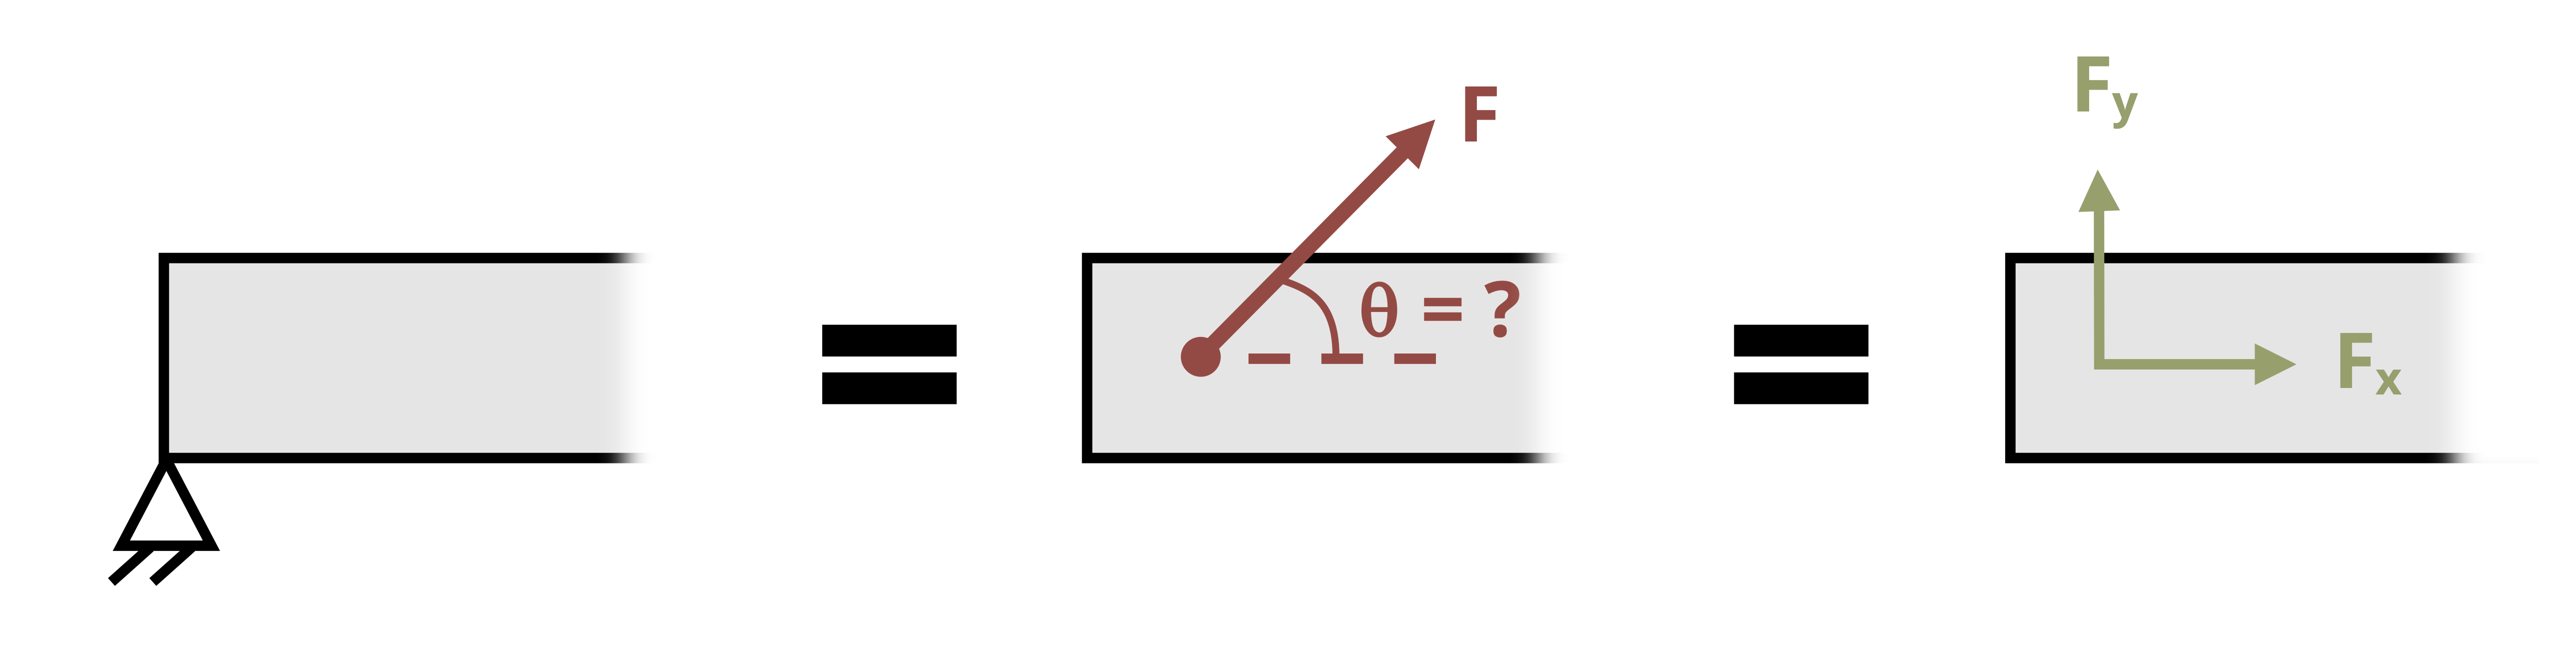
\includegraphics[width=93.75in,height=\textheight]{images/CH1 PNGs/table 1.1 part 1.png} \\
Normal supports

(including rollers, rockers, and smooth contact surface) & Force in the
direction normal to the support. Since the direction is known (normal to
the support), show as total force in the known direction. &
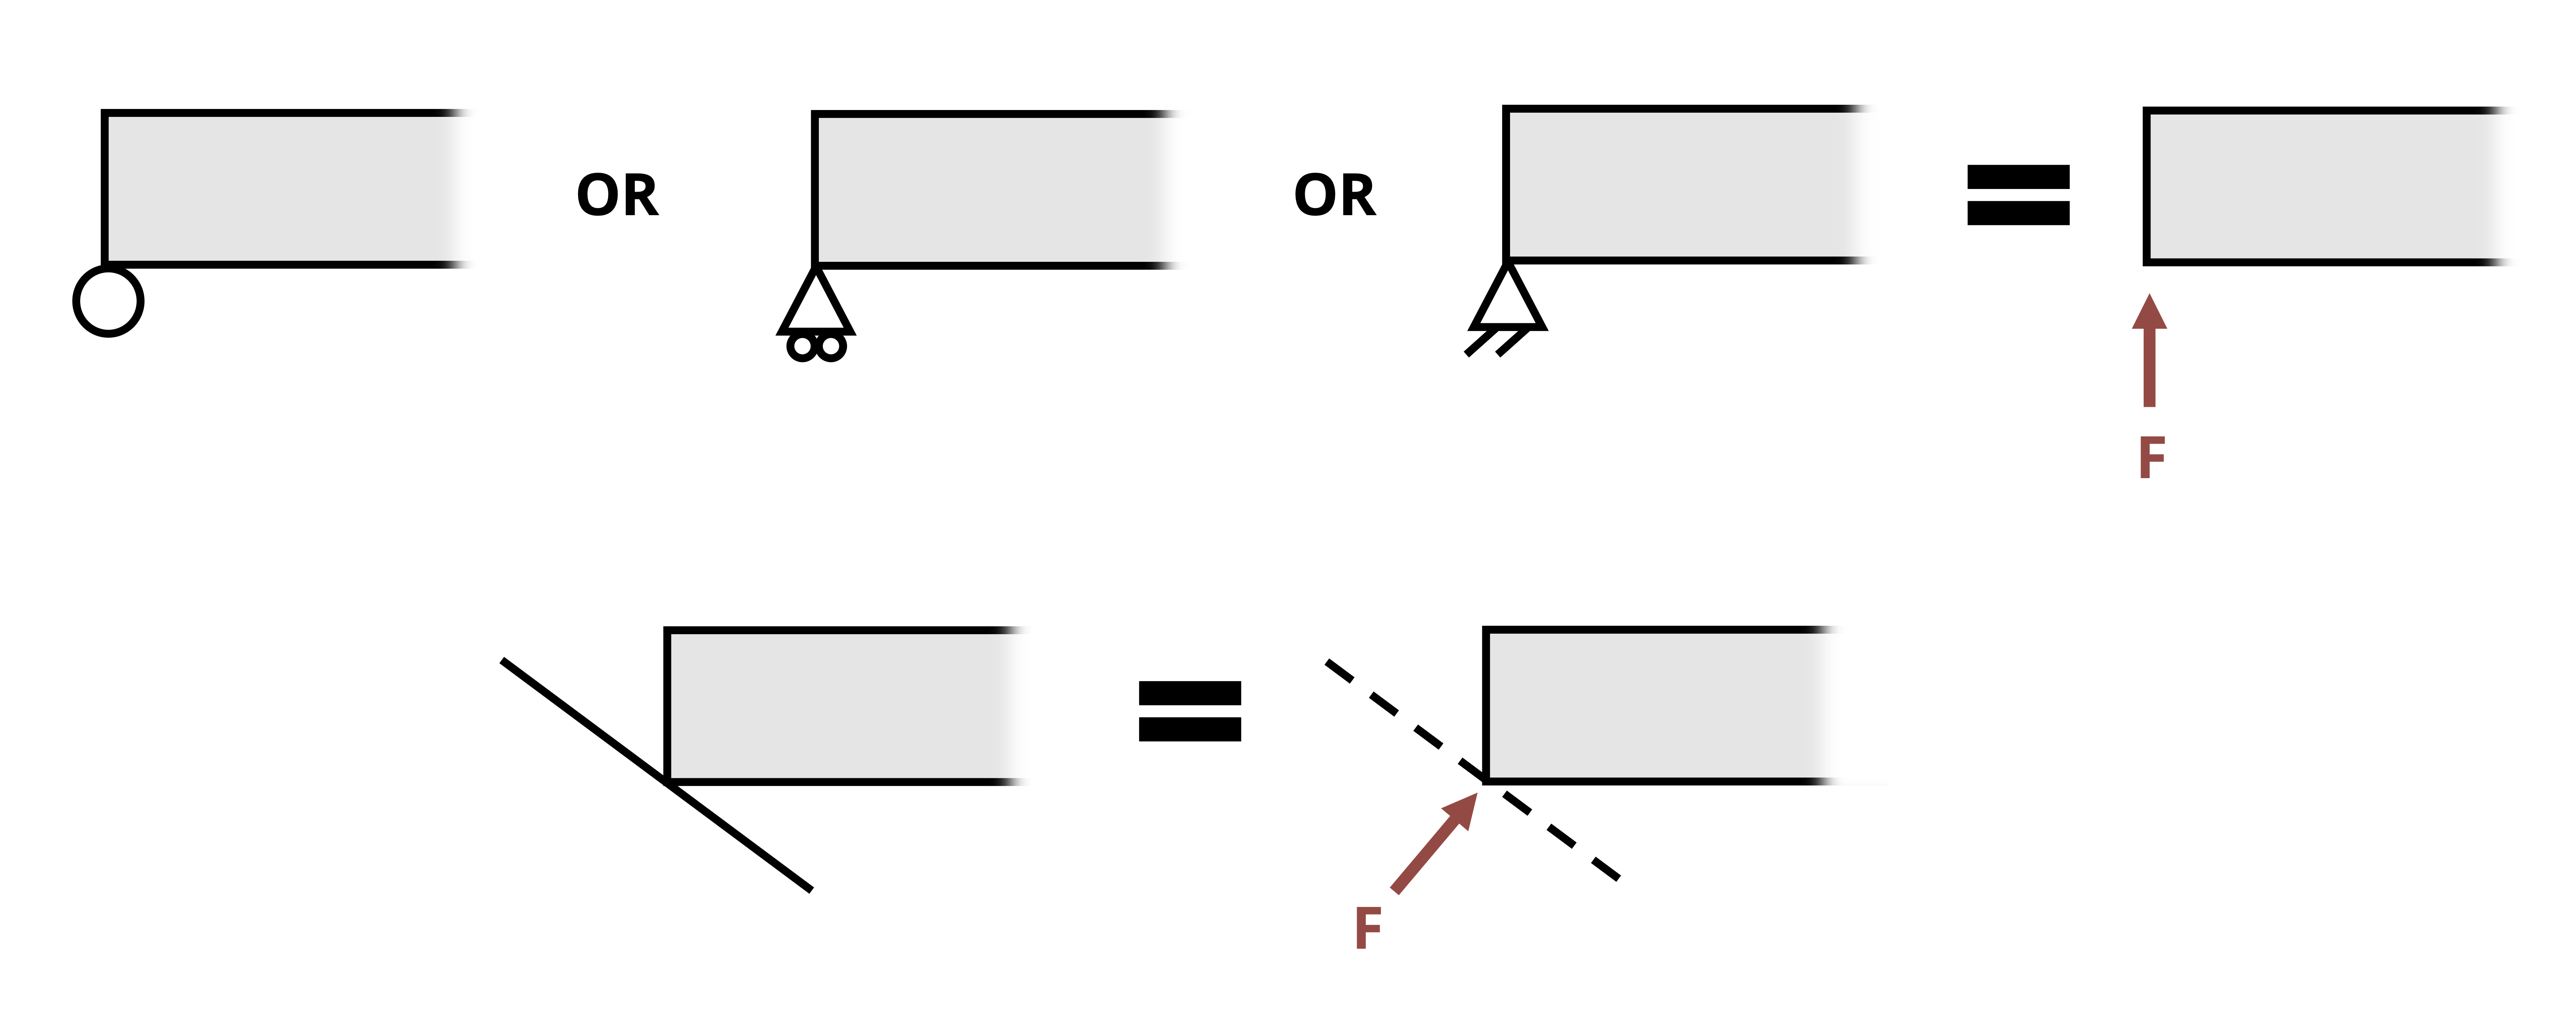
\includegraphics[width=93.75in,height=\textheight]{images/CH1 PNGs/table 1.1 part 2.png} \\
Cables & Force in the direction of the cable. Should always be drawn in
tension. &
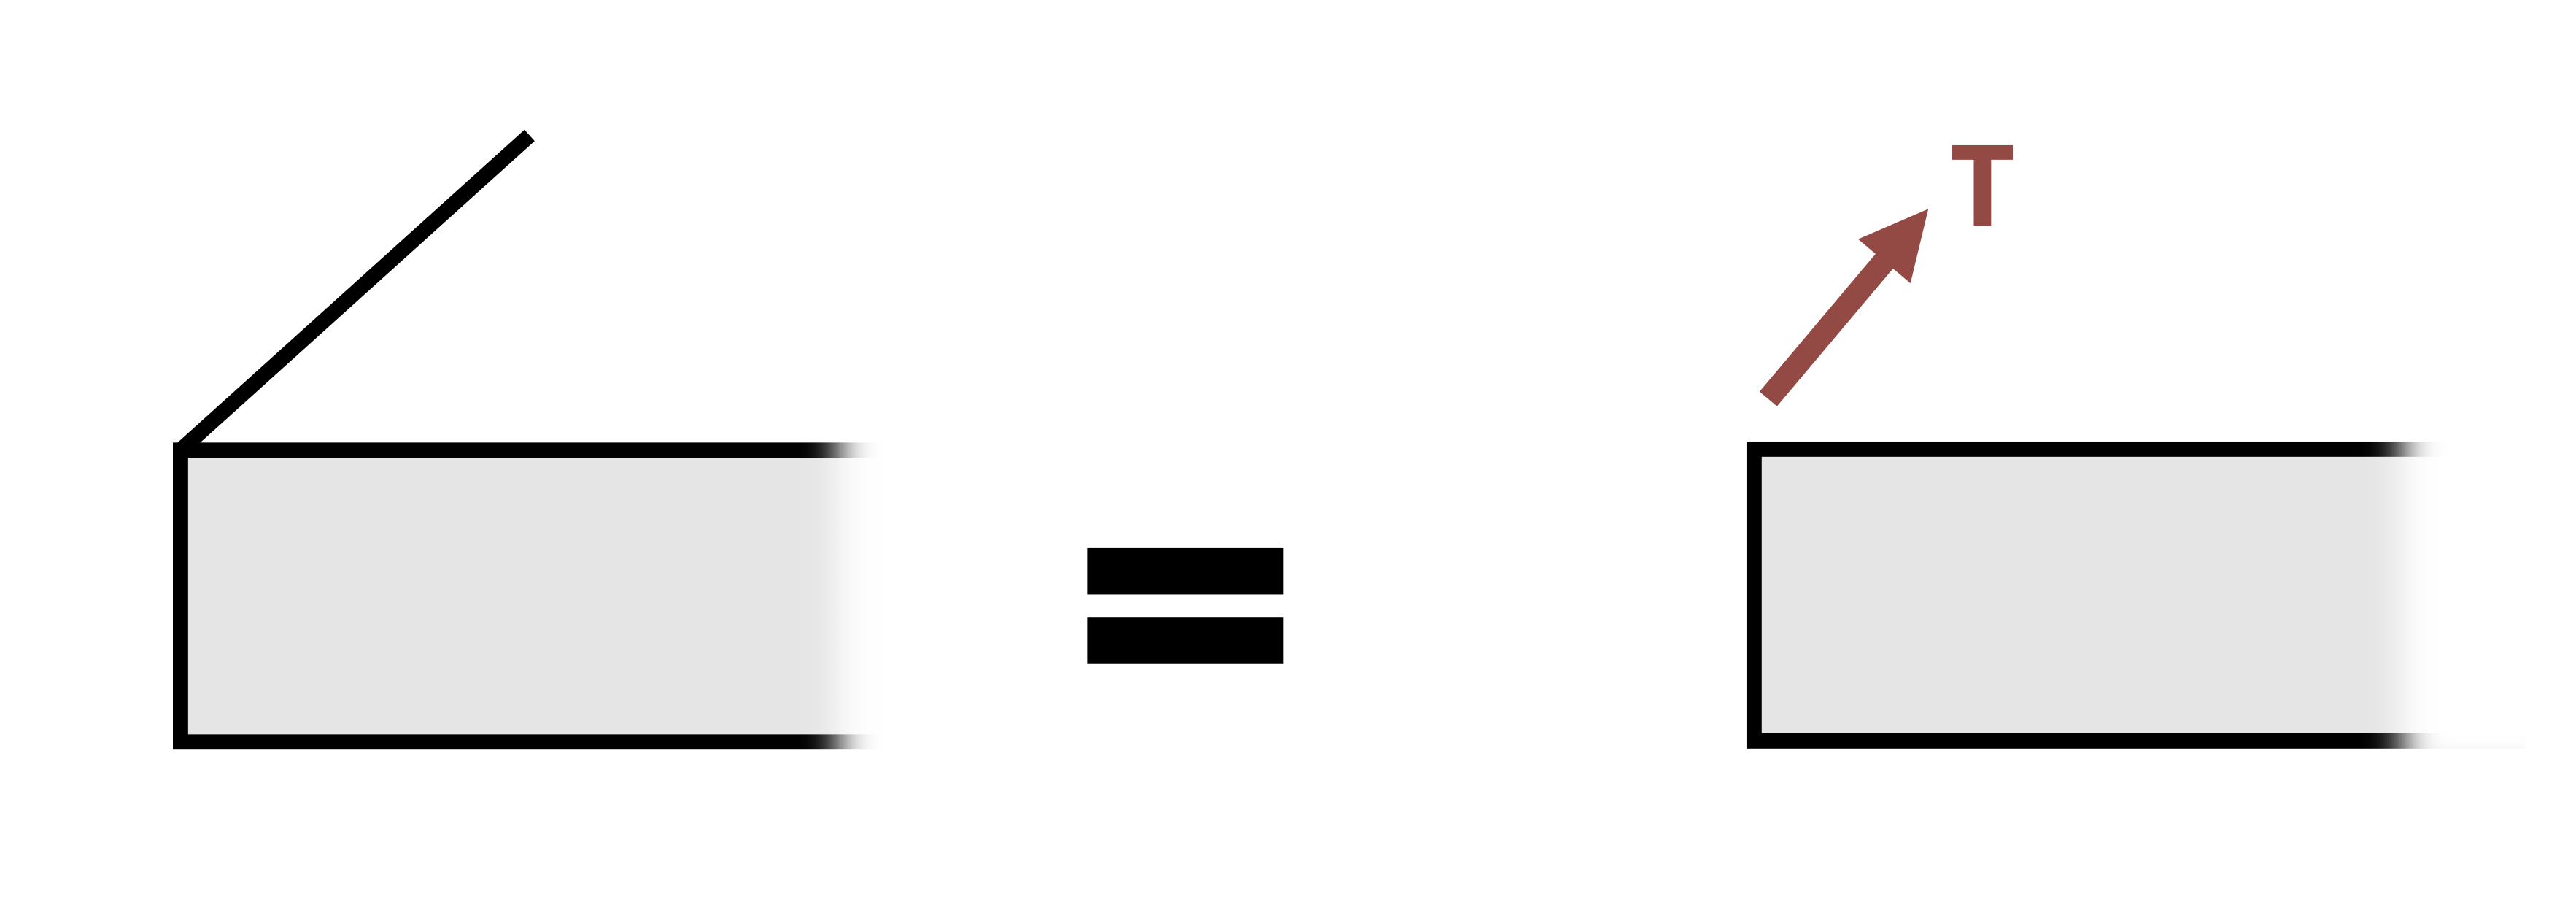
\includegraphics[width=93.75in,height=\textheight]{images/CH1 PNGs/table 1.1 part 3.png} \\
Fixed support & Force in an unknown direction (so draw x and y
components of force) as well as reaction couple moment &
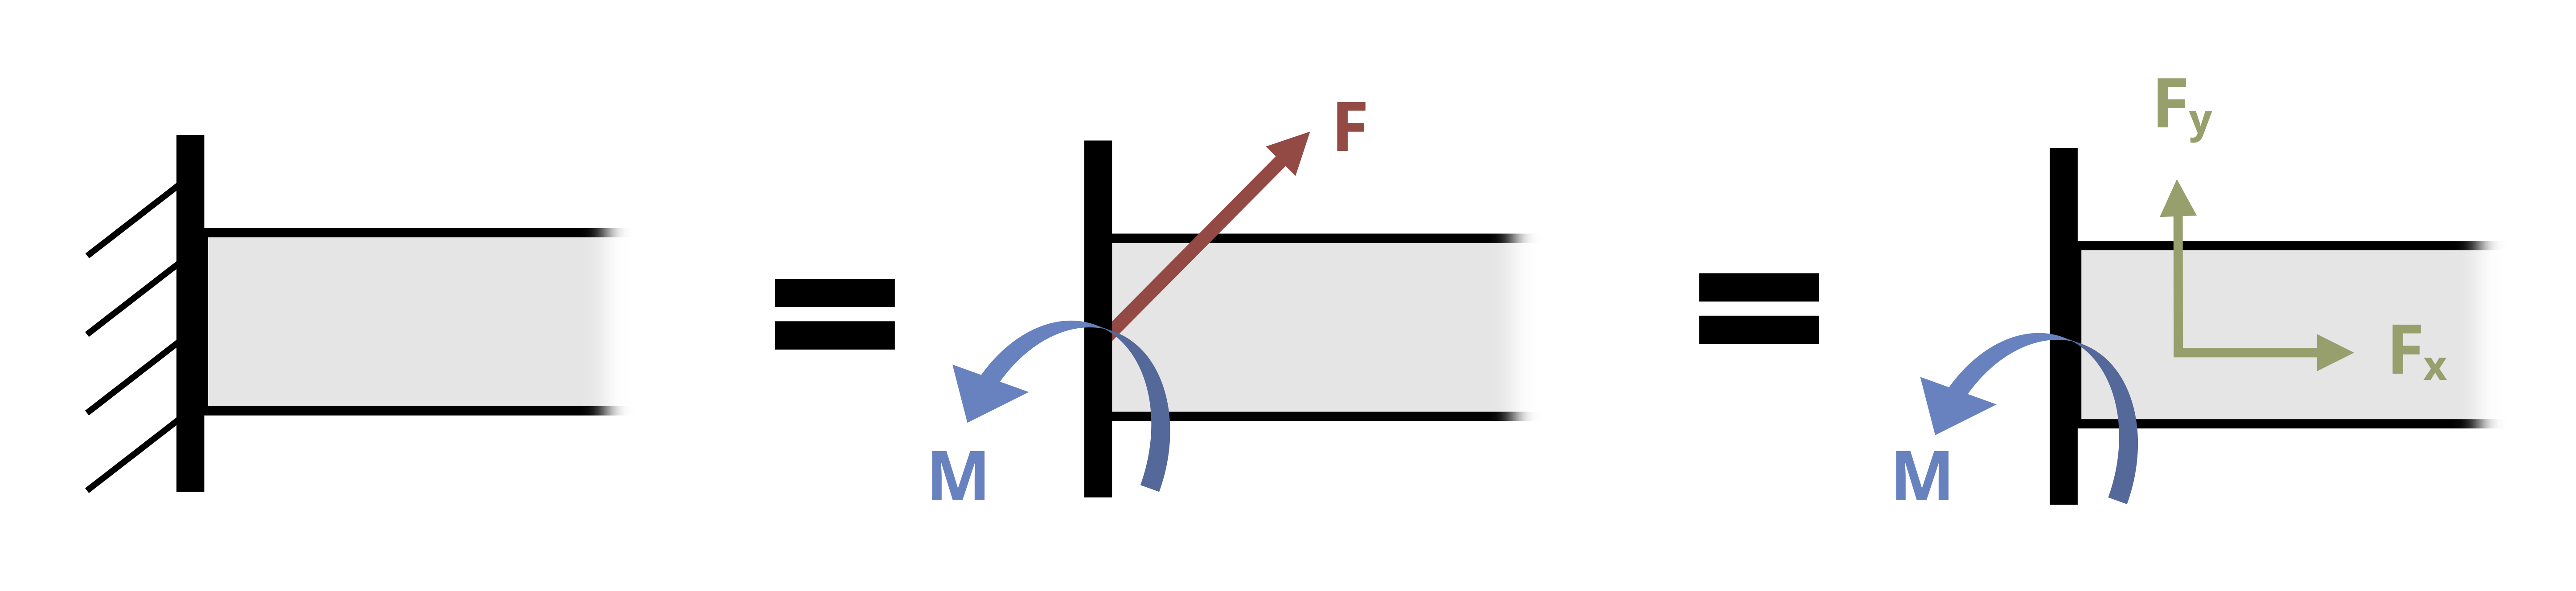
\includegraphics[width=93.75in,height=\textheight]{images/CH1 PNGs/table 1.1 part 4.png} \\
\end{longtable}

Notice that while pins and fixed supports react with a force in a
specific direction, both the magnitude and direction of the force are
unknown until equilibrium equations are applied to solve for them.
Instead of expressing the components of the unknown F in terms of the
unknown θ, the reactions are normally shown as the components
F\textsubscript{x} and F\textsubscript{y}. Once they are found, the
overall magnitude of the force in the pin and its direction can be
calculated
\(\left(F=\sqrt{F_x^2+F_y^2}, \tan \theta_x=\frac{F_y}{F_x}\right)\).

Section~\ref{sec-1_1} reviews equilibrium of members and frames in two
dimensions, including the analysis of two-force members and multi-force
members.

Section~\ref{sec-1.2} addresses internal loads, including normal force,
shear force, and bending moment.

Section~\ref{sec-1.3} reviews equilibrium in three dimensions.

\section{Equilibrium in Two Dimensions}\label{sec-1_1}

Click to expand

Once the FBD is drawn, the next step is to apply the equilibrium
equations. In two dimensions (x-y plane), these are:

\begin{equation}\phantomsection\label{eq-1.1}{
\boxed{\sum F_x=0 \quad \sum F_y=0 \quad \sum M_{any~point}=0}
}\end{equation}

Since there are three equations, a statically determinate problem should
have no more than 3 unknowns.

Example~\ref{exm-1.1} illustrates the process of finding external
reactions.

\begin{tcolorbox}[enhanced jigsaw, colback=white, colframe=quarto-callout-tip-color-frame, toptitle=1mm, arc=.35mm, bottomrule=.15mm, toprule=.15mm, opacitybacktitle=0.6, title={Example 1.1}, coltitle=black, breakable, colbacktitle=quarto-callout-tip-color!10!white, bottomtitle=1mm, titlerule=0mm, opacityback=0, leftrule=.75mm, left=2mm, rightrule=.15mm]

\begin{example}[]\protect\hypertarget{exm-1.1}{}\label{exm-1.1}

~

A 3 ft beam is supported by a pin connection at the wall at point A and
a cable at point C as shown. A load is applied 2 ft away from point A.
Find the force in pin A as well as the tensile force in the cable.

\begin{center}
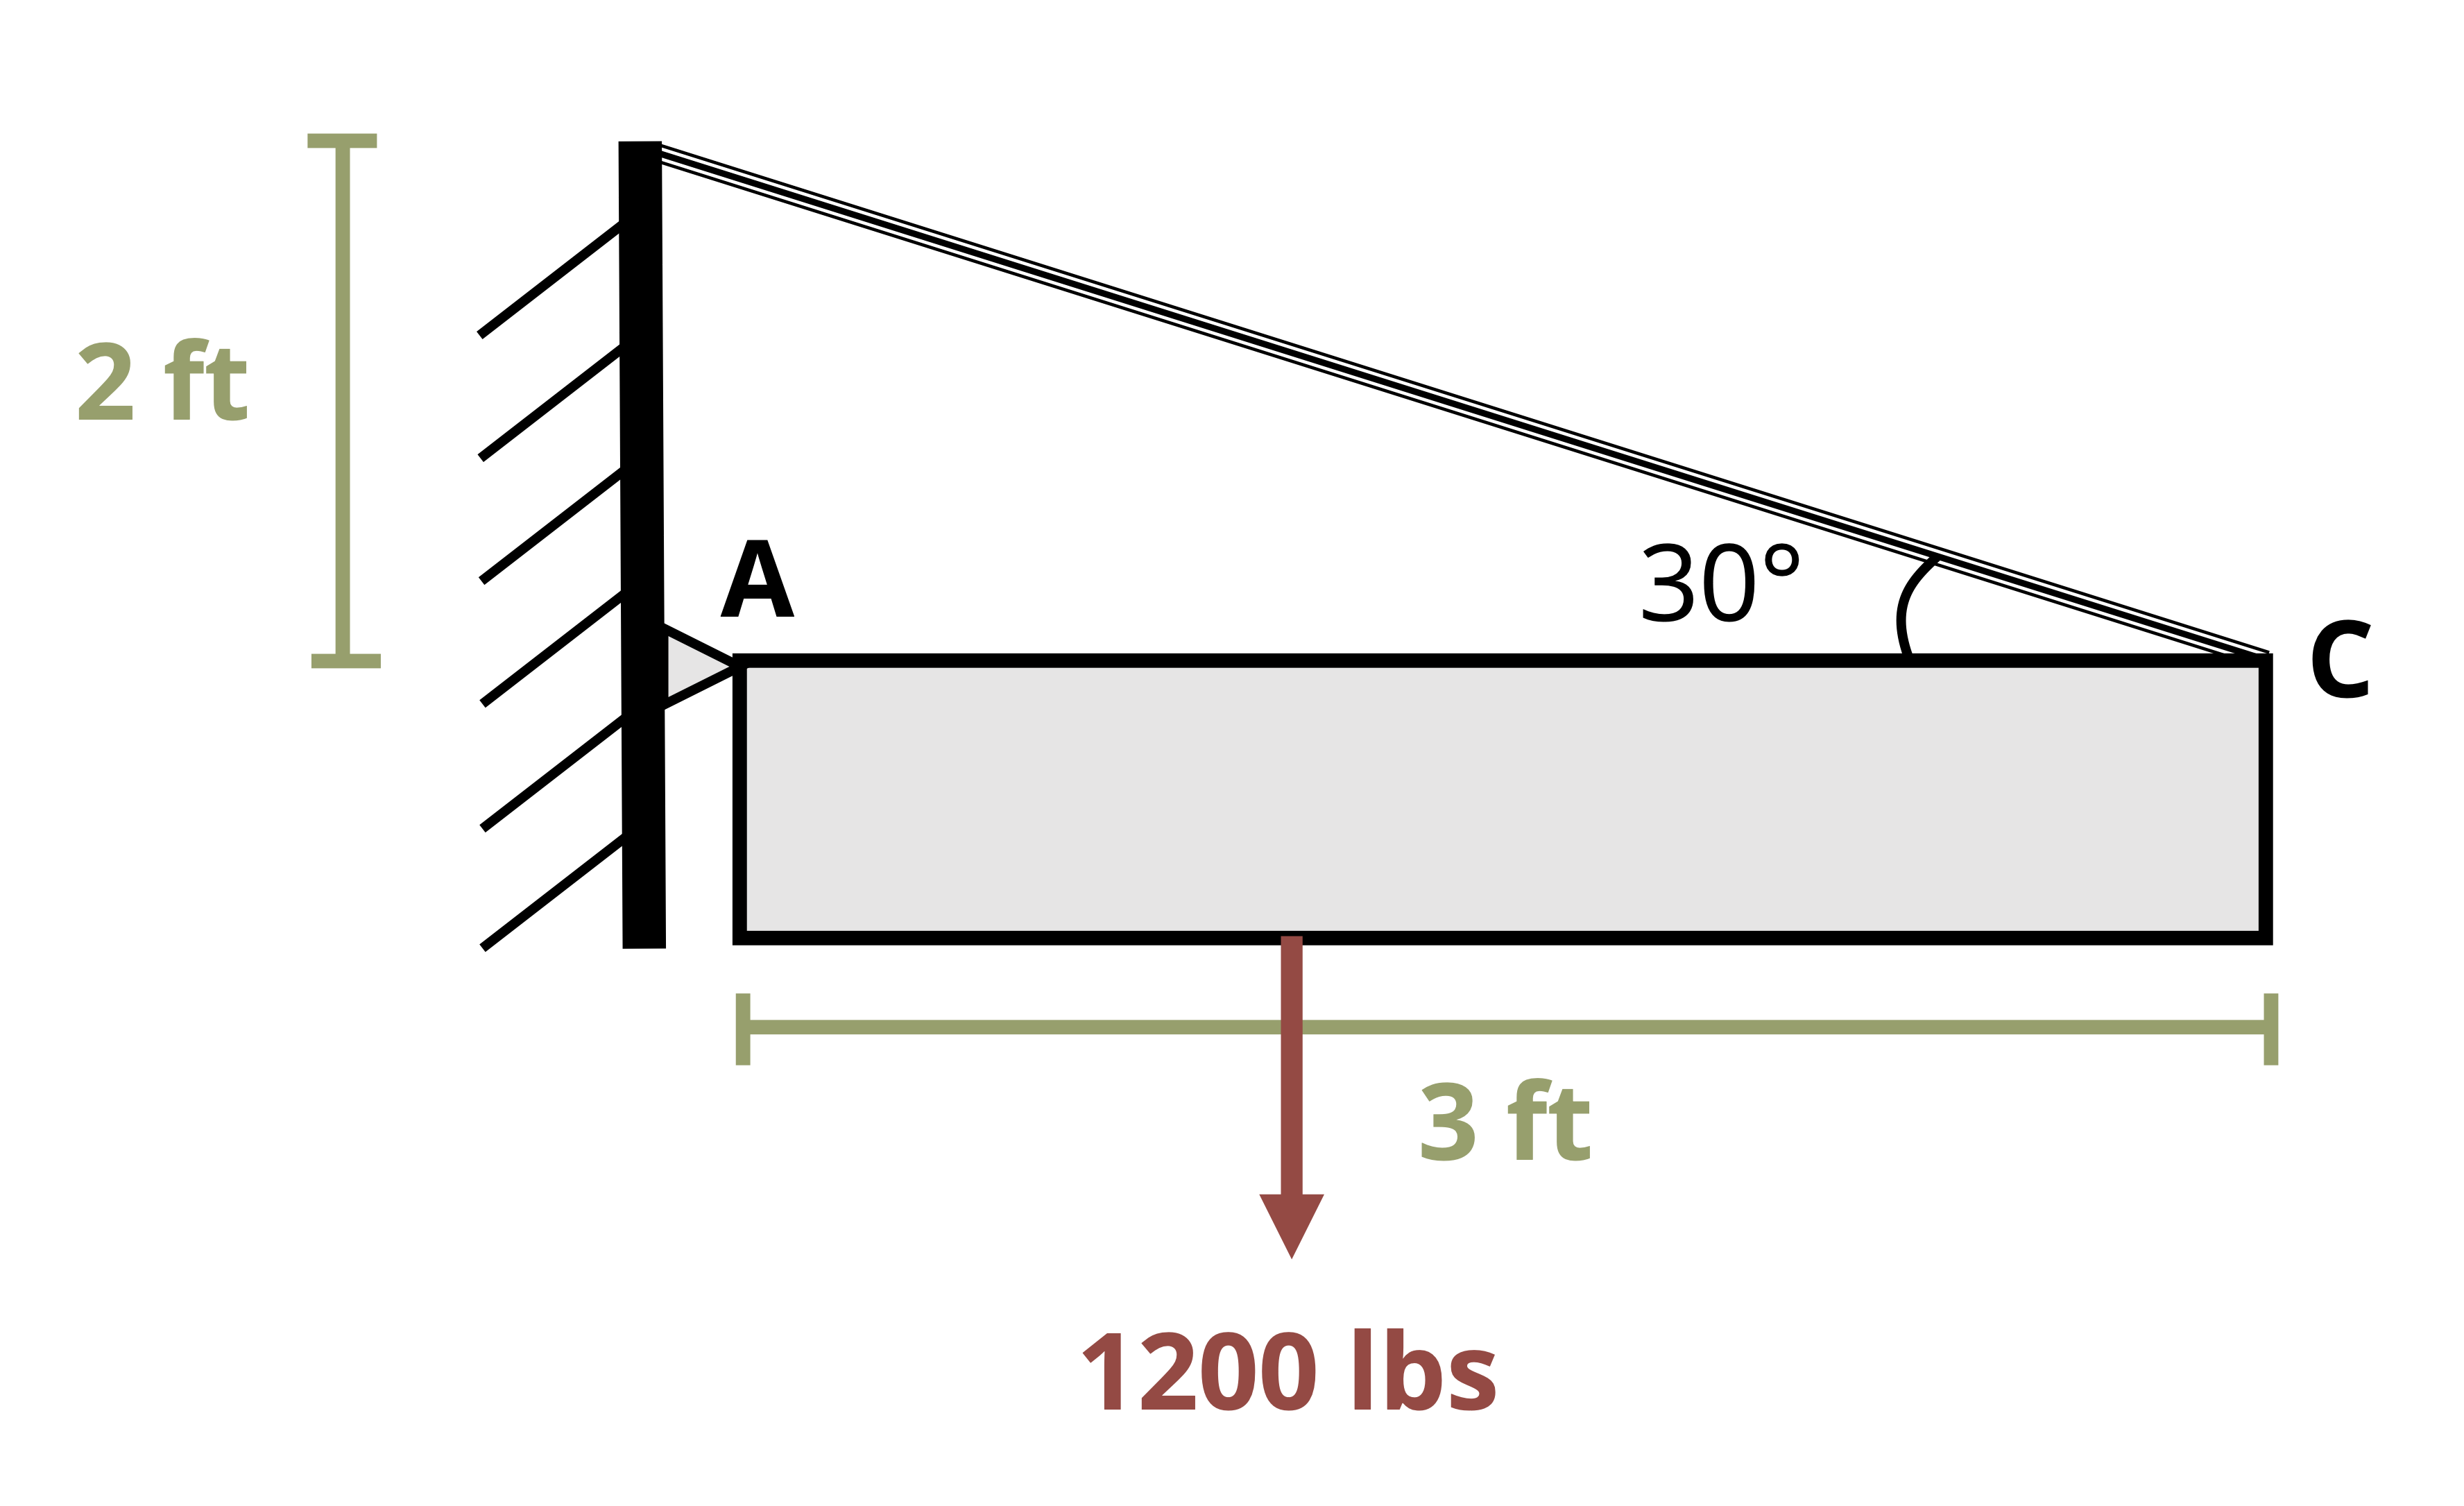
\includegraphics[width=2.75in,height=\textheight]{images/CH1 PNGs/example 1.1 part 1.png}
\end{center}

\begin{tcolorbox}[enhanced jigsaw, colback=white, colframe=quarto-callout-tip-color-frame, toptitle=1mm, arc=.35mm, bottomrule=.15mm, toprule=.15mm, opacitybacktitle=0.6, title={Solution}, coltitle=black, breakable, colbacktitle=quarto-callout-tip-color!10!white, bottomtitle=1mm, titlerule=0mm, opacityback=0, leftrule=.75mm, left=2mm, rightrule=.15mm]

\textbf{Step 1: Draw the FBD}

Note that a guess needs to be made for the positive or negative sense of
A\textsubscript{x} and A\textsubscript{y}, but the tensile force from a
cable should always be shown to pull away from the body. The correct
sense of A\textsubscript{x} and A\textsubscript{y} will be determined by
obtaining positive or negative answers for the values. A positive answer
means the direction was correctly assumed and a negative answer means
the force should be in the opposite direction.

\begin{center}
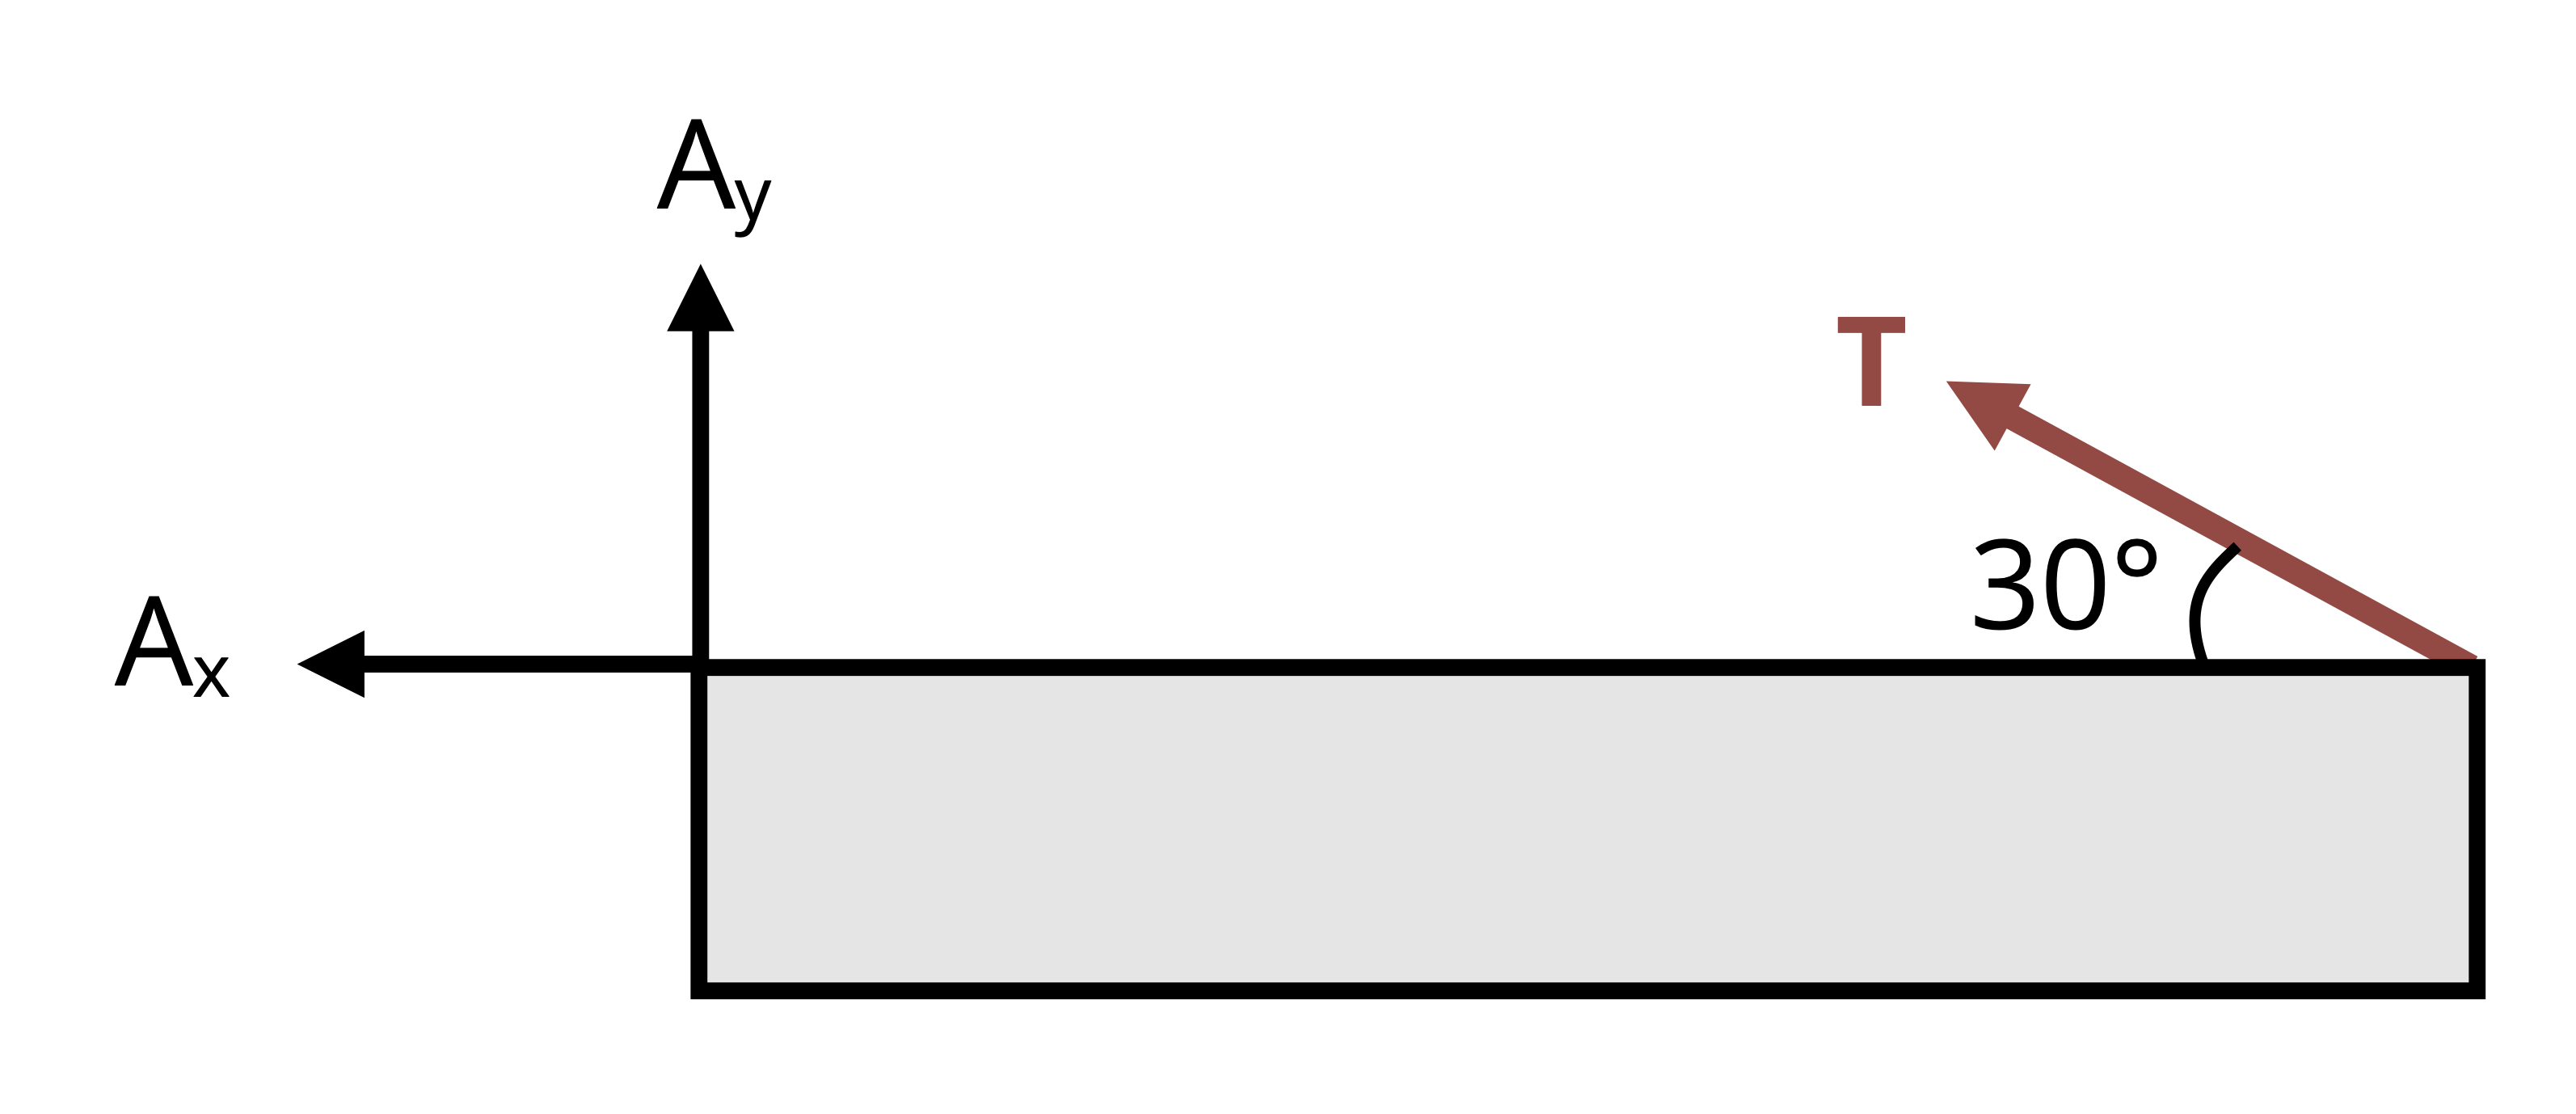
\includegraphics[width=2.64583in,height=\textheight]{images/CH1 PNGs/example 1.1 part 2.png}
\end{center}

\textbf{Step 2: Apply equilibrium equations}

Starting with the moment about A will eliminate two unknowns from the
equation so that tensile force T can be solved for. Then substitute the
result from T into the other two equations to find A\textsubscript{x}
and A\textsubscript{y}.

\[
\begin{aligned}
& \sum M_A=T \sin (30^{\circ}) * 3{~ft}-1,200{~lb }*2{~ft}=0 \quad\rightarrow\quad T=1,600 {~lb} \\
& \sum F_x=-A_x-T \cos (30^{\circ})=0 \quad\rightarrow\quad A_x=-1,384.6{~lb} \\
& \sum F_y=A_y+T \sin (30^{\circ})-1200{~lb}=0 \quad\rightarrow\quad A_y= 400{~lb}
\end{aligned}
\]

Since a negative answer was obtained for A\textsubscript{x}, that force
actually acts in the positive x direction.

The total force in pin A is then \(F_A=\sqrt{A_x^2+A_y^2}=1,441{~lb}\)

\textbf{Answer: T = 1,600 lb, FA = 1,441 lb}

\end{tcolorbox}

\end{example}

\end{tcolorbox}

\subsection{Two Force Members}\label{two-force-members}

One special type of pin connection for which the direction of the
reaction force is known is one in which the pin is connected to a
\textbf{two-force member}. Contrary to the name, a two-force member is
not necessarily a member on which only two forces are applied, but
rather it is a member on which forces are applied at only two locations.
A two-force member can be any shape, as is demonstrated in
Figure~\ref{fig-1.1}. One easy way to recognize a two-force member is to
note the presence of only two connection points (such as two pins) but
no other locations at which a force or moment couple is applied. Once a
member is recognized to be a two-force member, it can be concluded that
the resultant force at both connection points will be equal in magnitude
(so F\textsubscript{A} = F\textsubscript{B} in Figure~\ref{fig-1.1}) and
opposite in direction and follow a line of action that goes through the
connections. For a straight member, it can also be concluded that the
force within the two-force member (internal reaction as will be
discussed in Section~\ref{sec-1_1}) is equal to the reaction force in
the pin.

\begin{figure}

\centering{

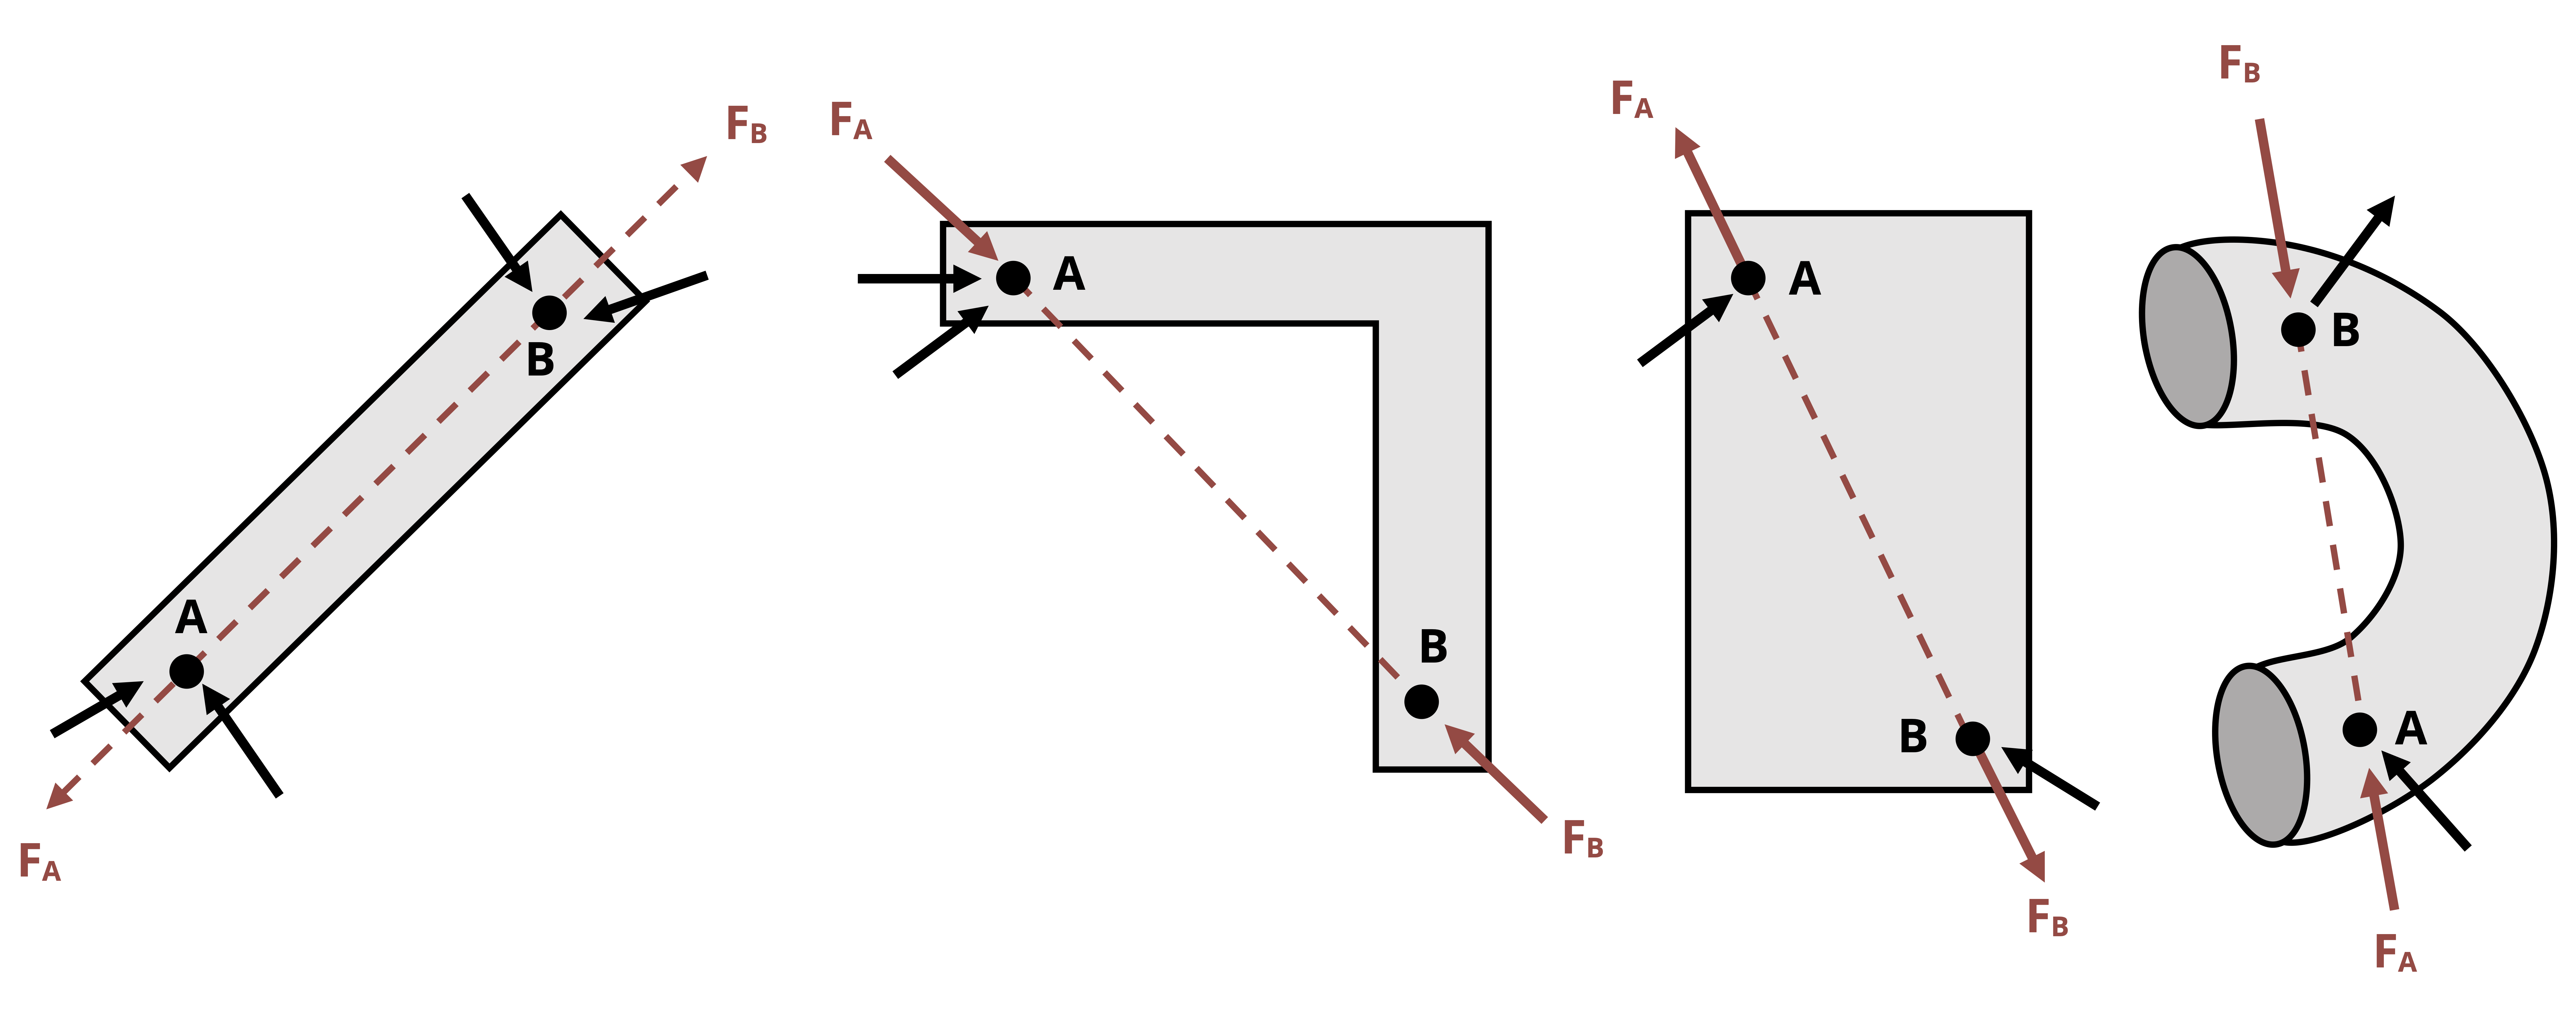
\includegraphics[width=6.6875in,height=\textheight]{images/CH1 PNGs/figure 1.1.png}

}

\caption{\label{fig-1.1}Illustrations of two force members showing the
line of action of the reaction force passing through the joints. Note
that F\textsubscript{A} = F\textsubscript{B}.}

\end{figure}%

The presence and recognition of two force members can make some
otherwise statically indeterminate problems become statically
determinate. This is demonstrated in Example~\ref{exm-1.2} below.

\begin{tcolorbox}[enhanced jigsaw, colback=white, colframe=quarto-callout-tip-color-frame, toptitle=1mm, arc=.35mm, bottomrule=.15mm, toprule=.15mm, opacitybacktitle=0.6, title={Example 1.2}, coltitle=black, breakable, colbacktitle=quarto-callout-tip-color!10!white, bottomtitle=1mm, titlerule=0mm, opacityback=0, leftrule=.75mm, left=2mm, rightrule=.15mm]

\begin{example}[]\protect\hypertarget{exm-1.2}{}\label{exm-1.2}

~

Determine the force in pin C and in pin A.

\begin{center}
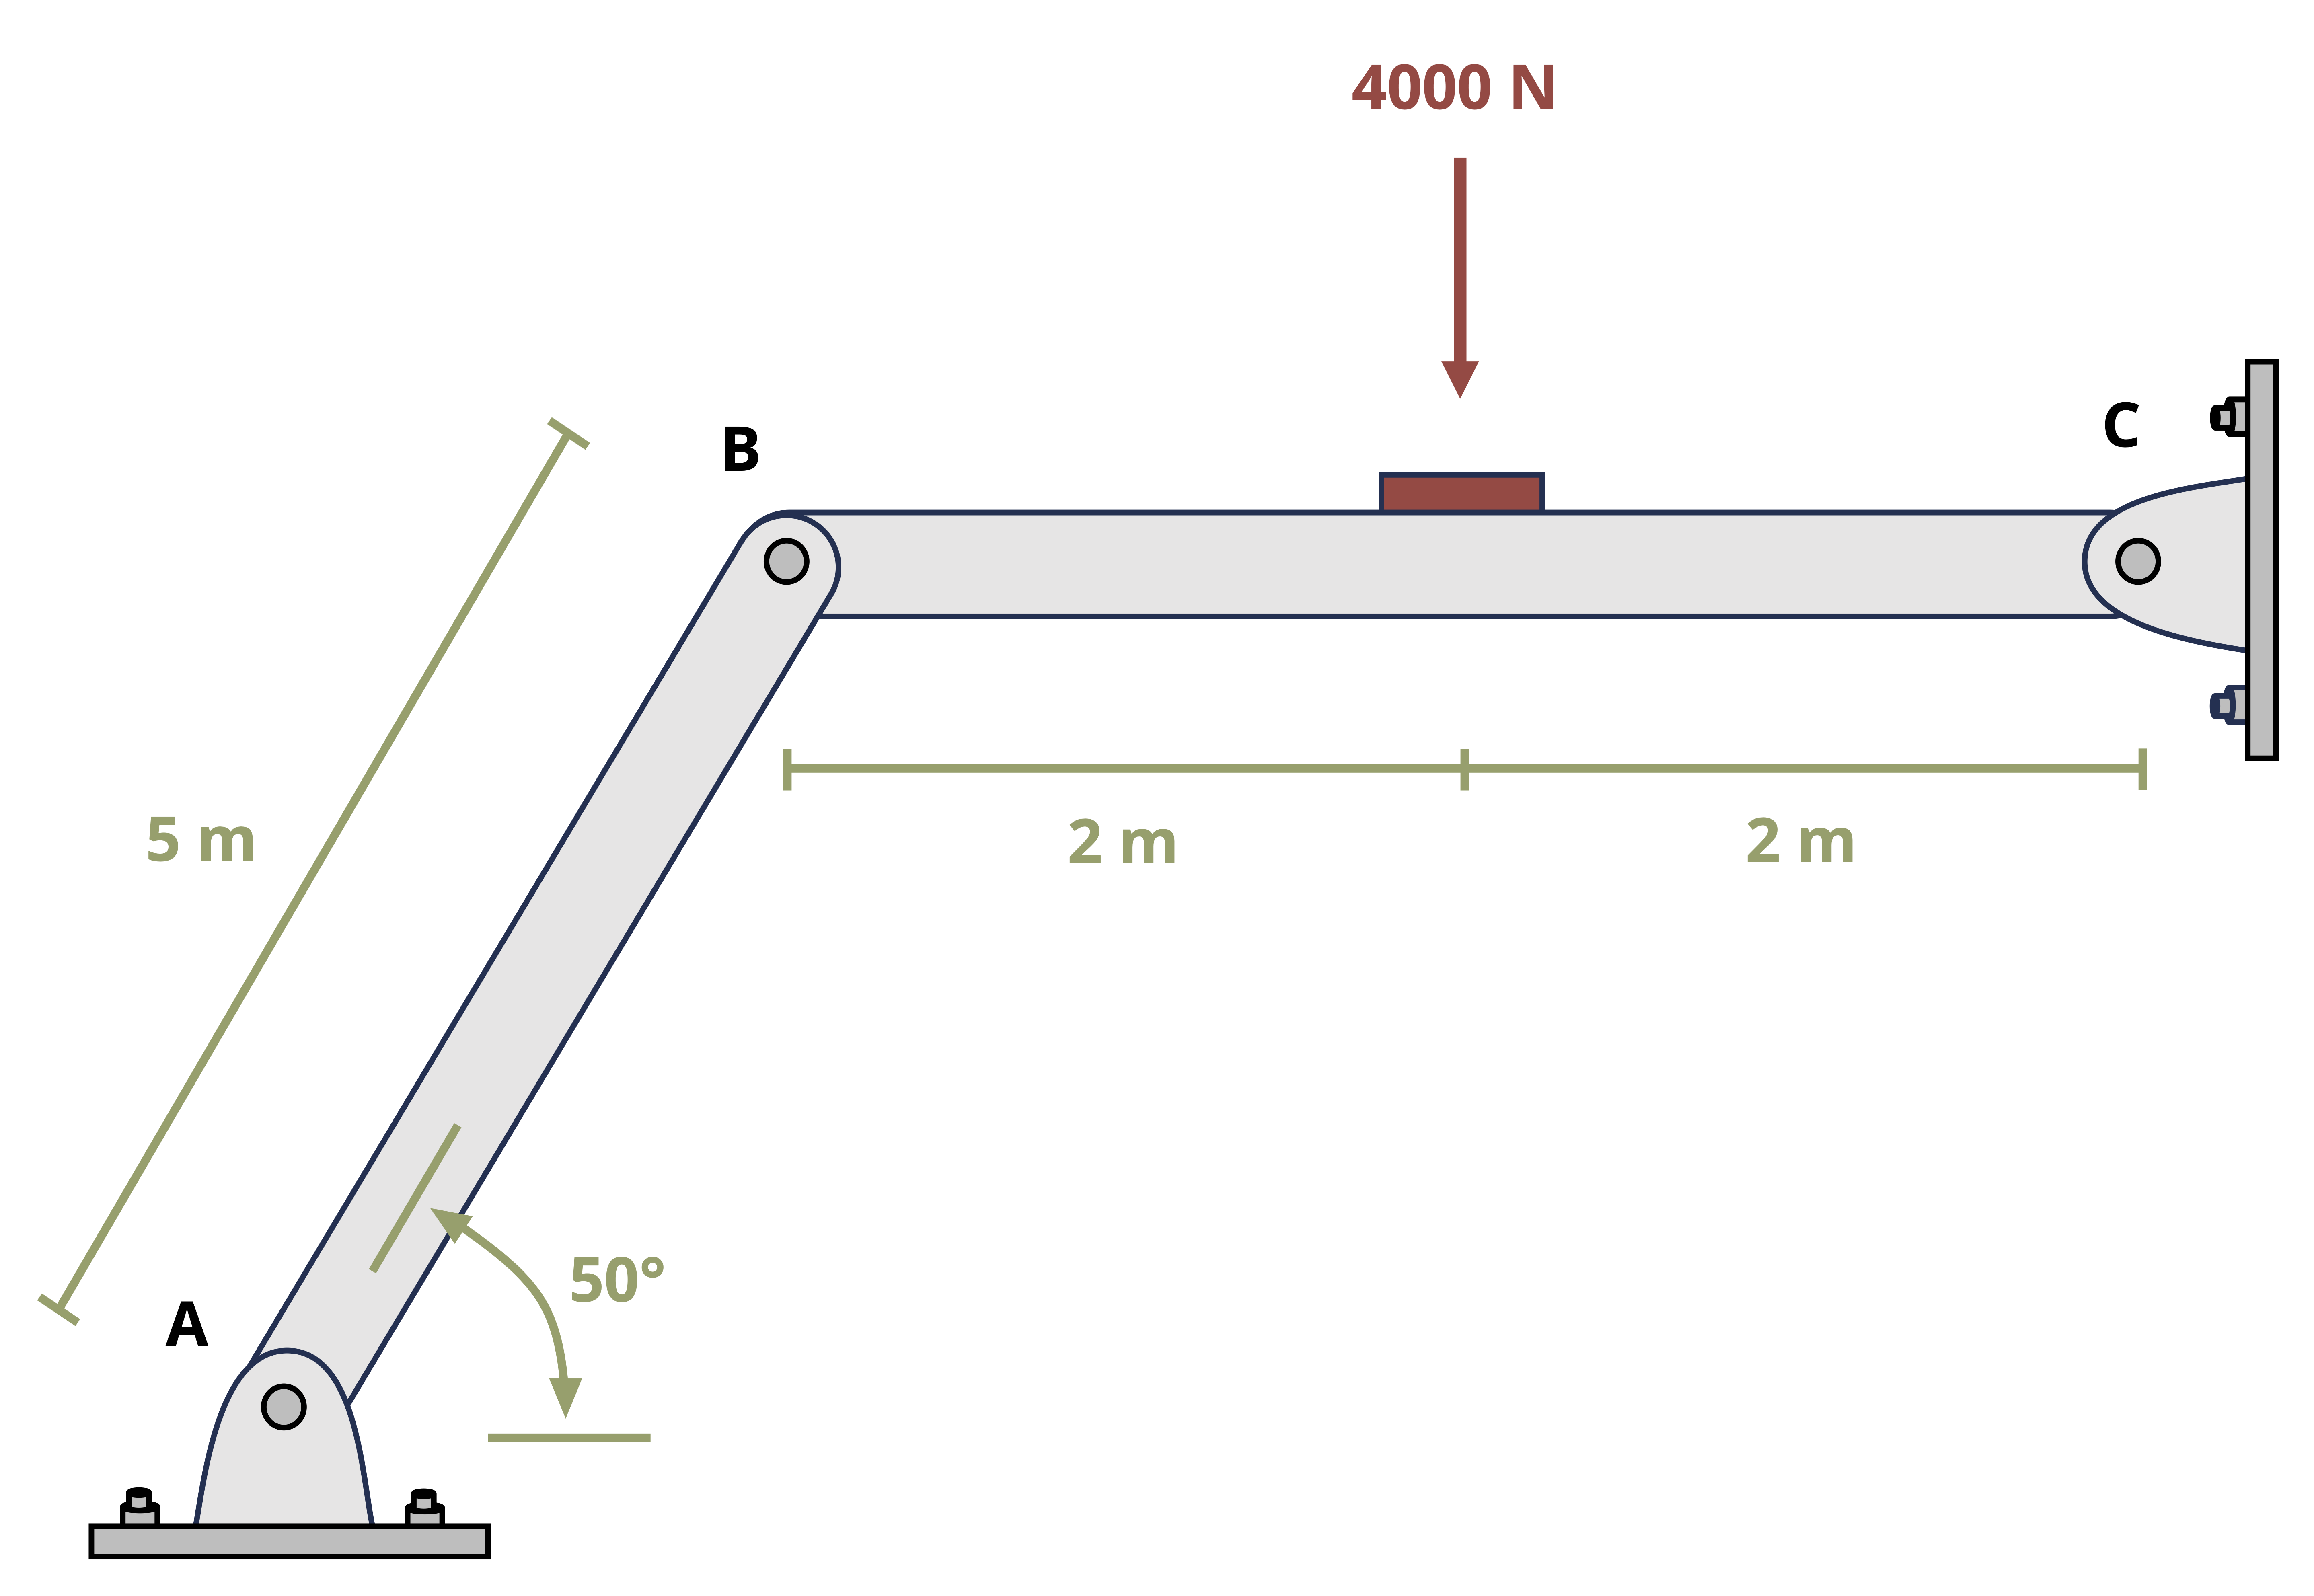
\includegraphics[width=4.58333in,height=\textheight]{images/Updated CH1 examples/example 1.2 part 1.png}
\end{center}

\begin{tcolorbox}[enhanced jigsaw, colback=white, colframe=quarto-callout-tip-color-frame, toptitle=1mm, arc=.35mm, bottomrule=.15mm, toprule=.15mm, opacitybacktitle=0.6, title={Solution}, coltitle=black, breakable, colbacktitle=quarto-callout-tip-color!10!white, bottomtitle=1mm, titlerule=0mm, opacityback=0, leftrule=.75mm, left=2mm, rightrule=.15mm]

\textbf{Step 1: Draw the FBD}

\begin{center}
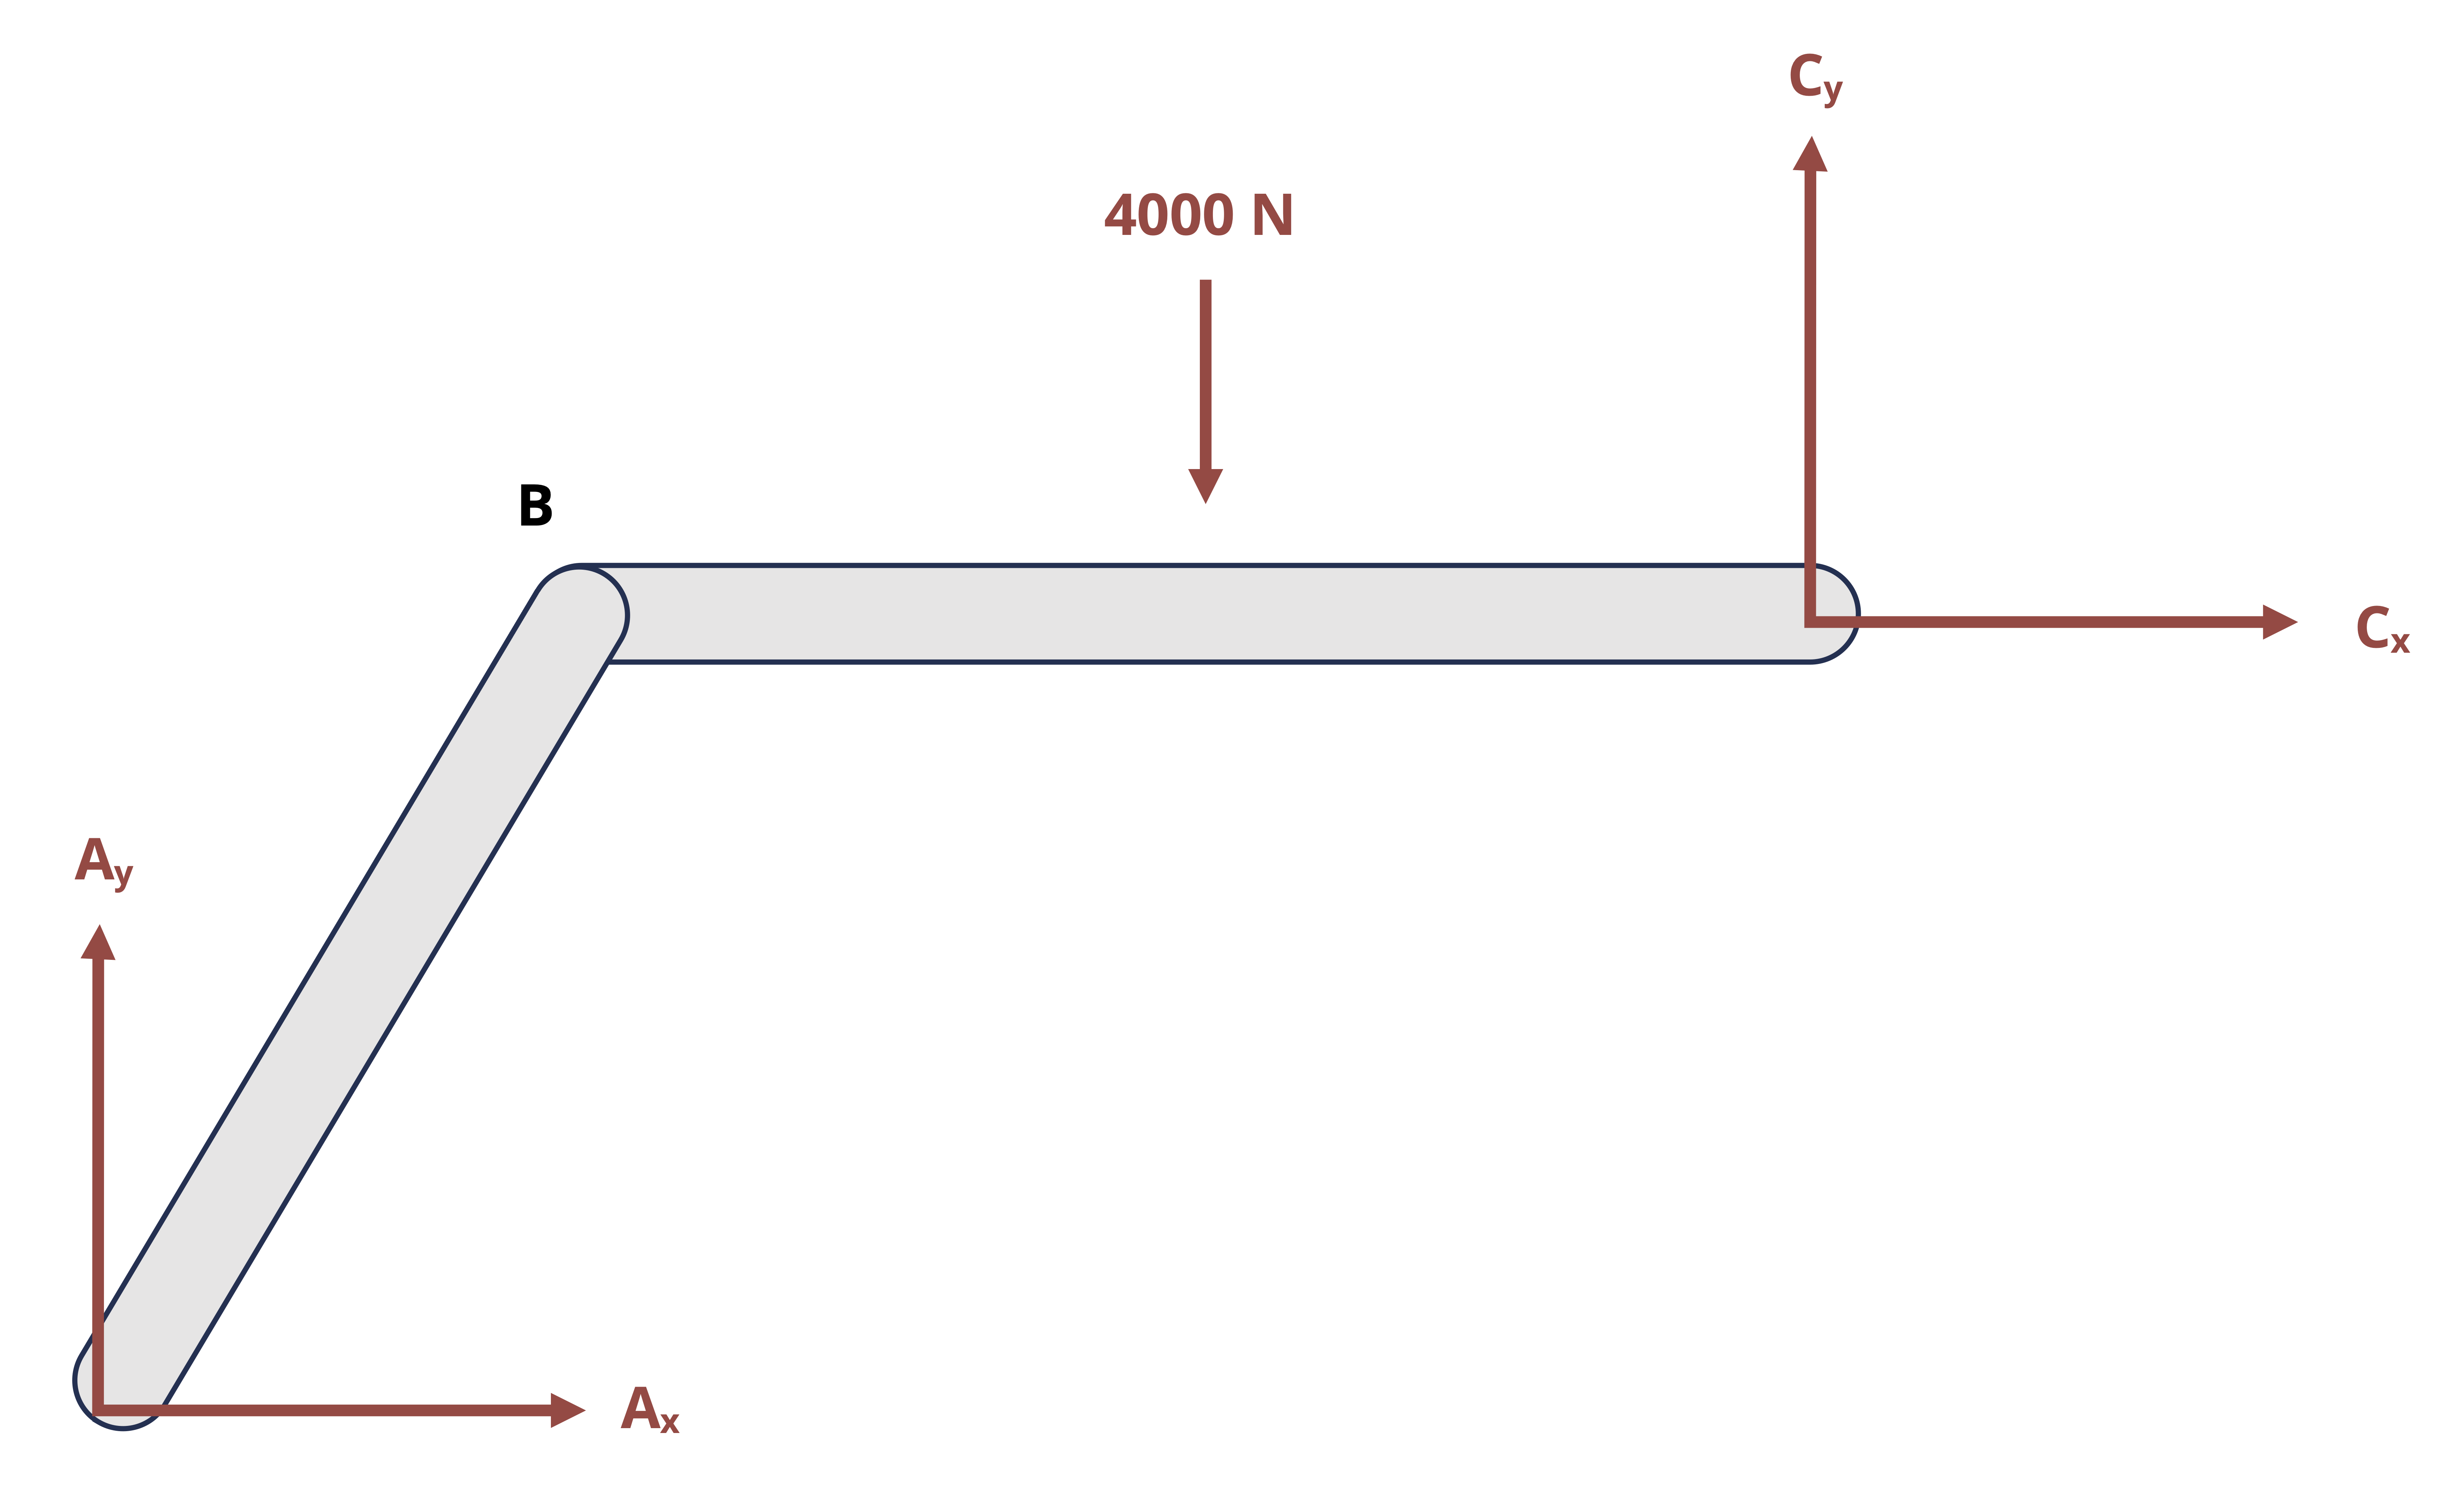
\includegraphics[width=4.91667in,height=\textheight]{images/Updated CH1 examples/example 1.2 part 2.png}
\end{center}

Based on this FBD, it appears that there are 4 unknowns and therefore
not solvable by just 3 equilibrium equations. However, recognizing that
bar AB is a two-force member (since there is a pin at A and a pin at B
but no other forces acting on that bar), it can be taken as known that
the line of action of the reaction force at A goes through points A and
B. Thus, the FBD can be redrawn with just 3 unknowns:

\begin{center}
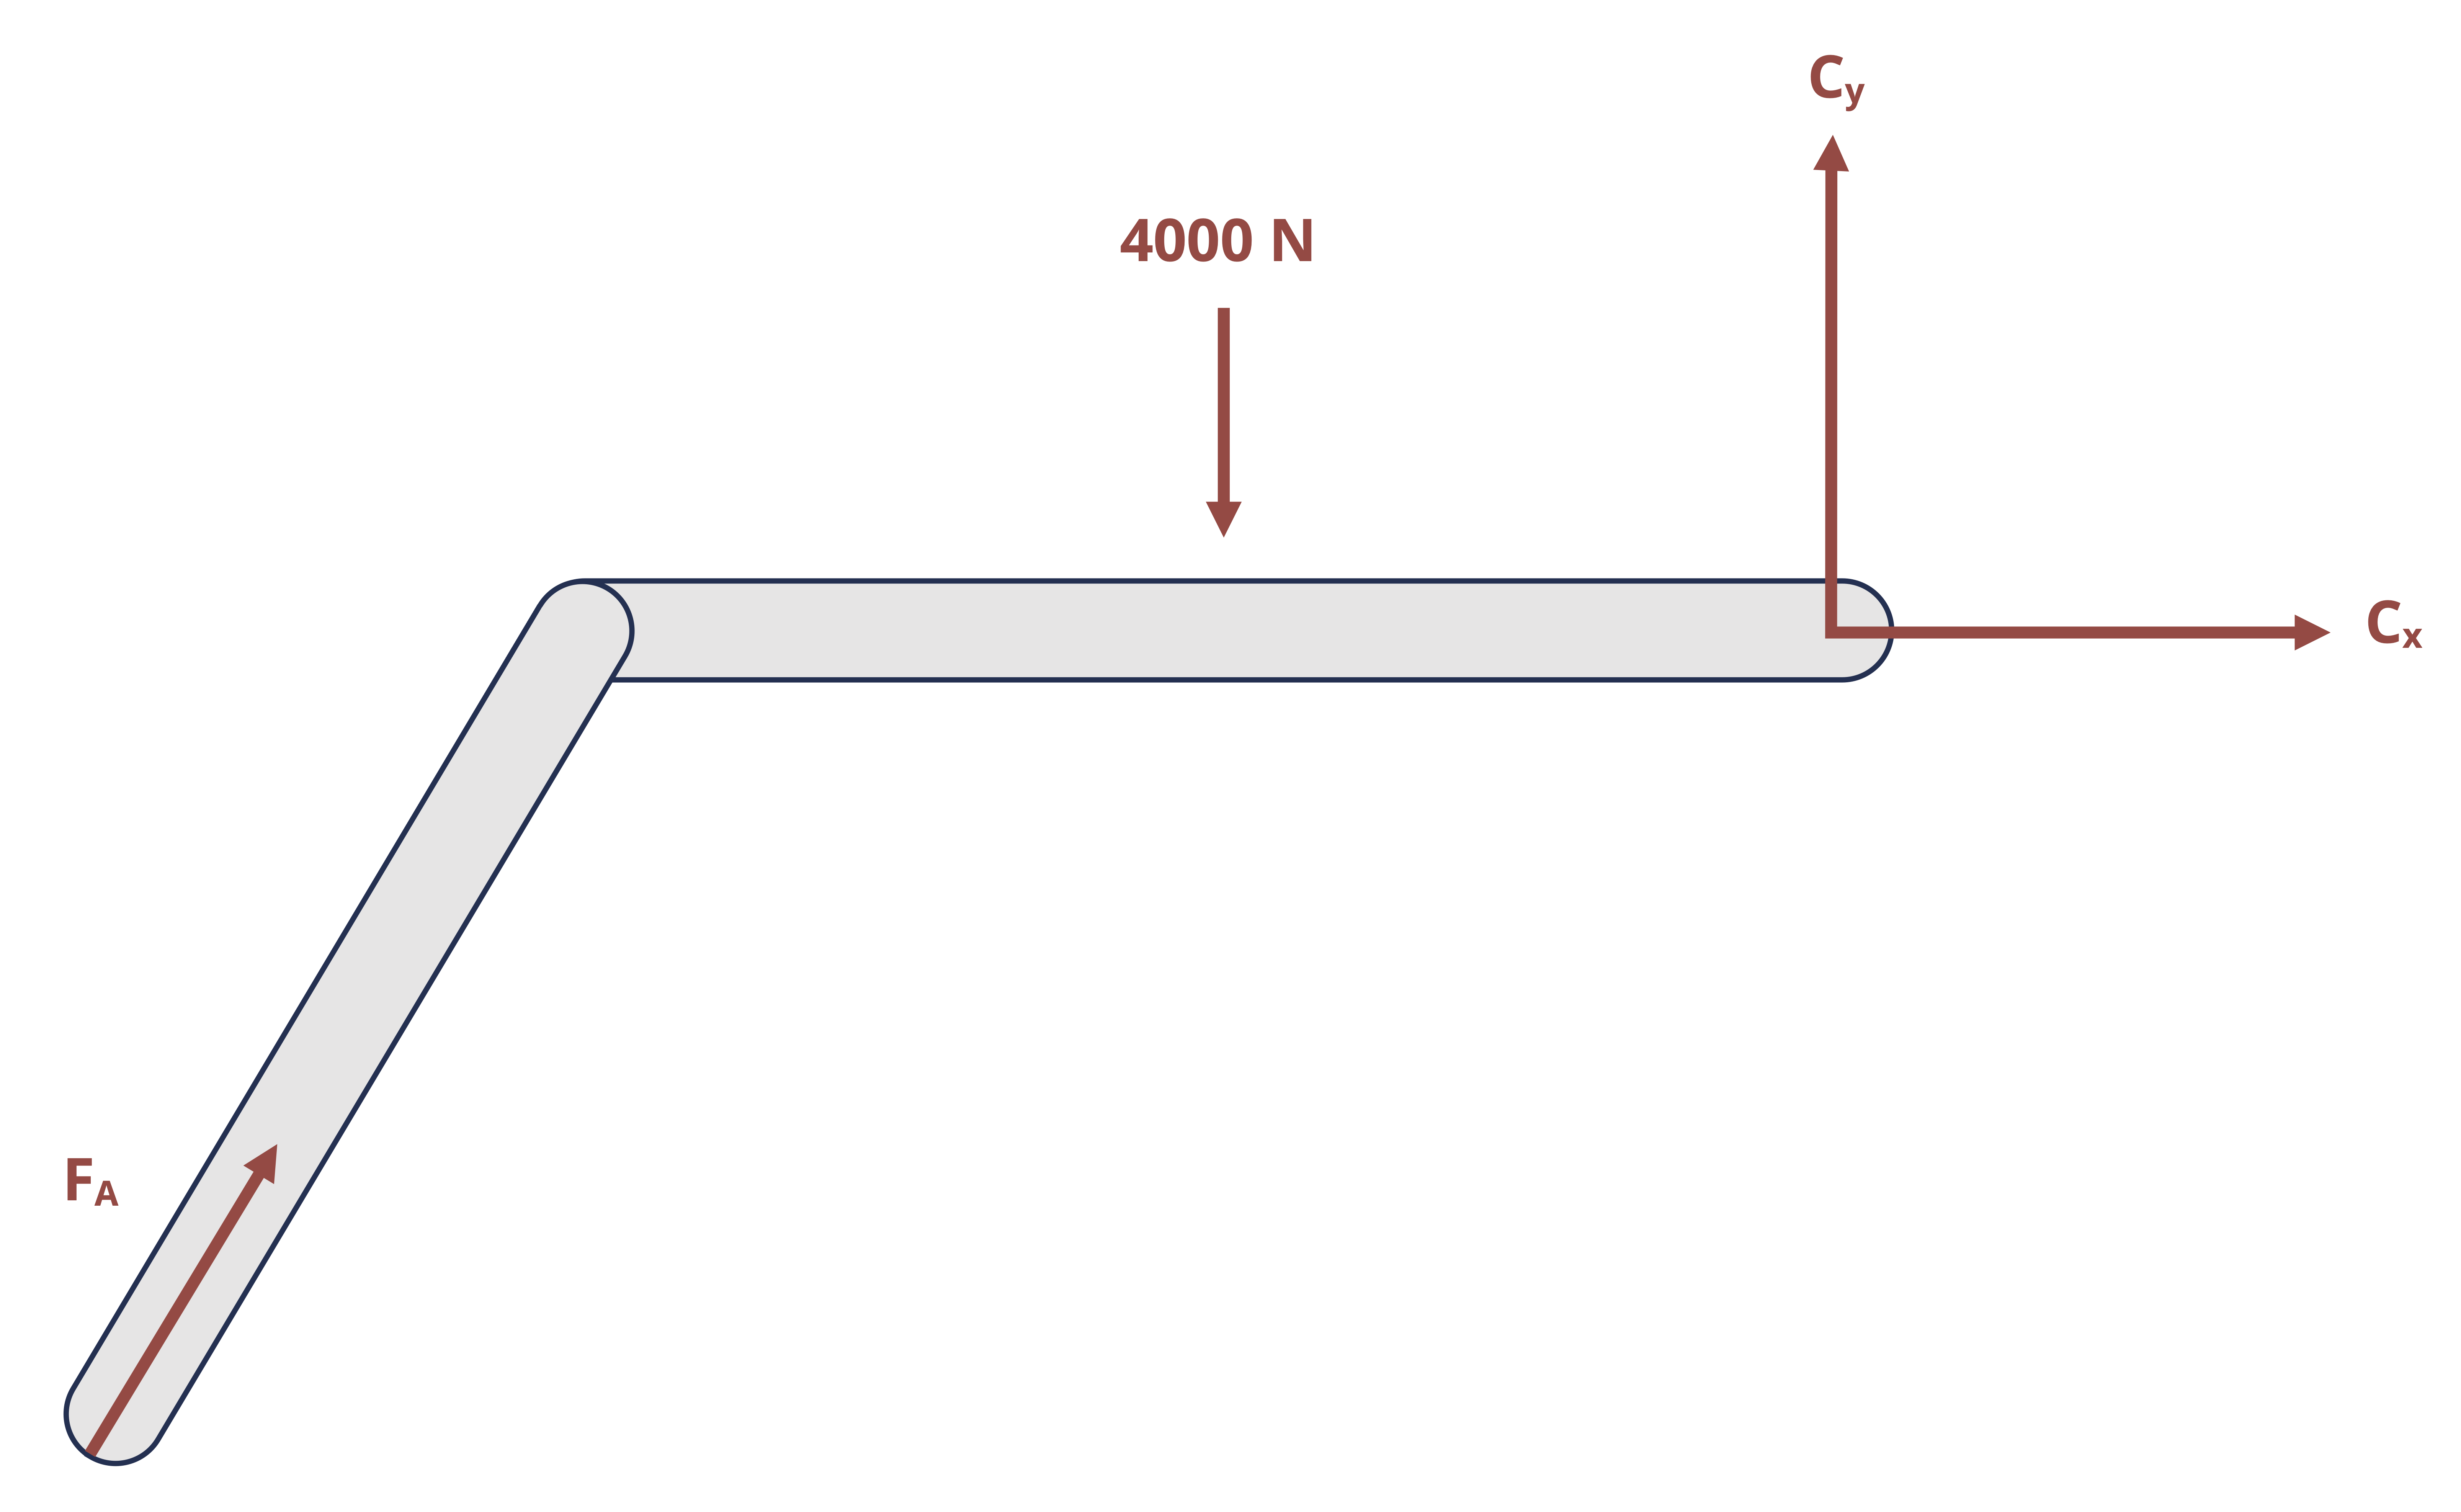
\includegraphics[width=3.03125in,height=\textheight]{images/Updated CH1 examples/example 1.2 part 3.png}
\end{center}

\textbf{Step 2: Apply equilibrium equations}

\[
\begin{aligned}
& \sum M_C=F_A \cos \left(50^{\circ}\right)*(5{~m}) \sin \left(50^{\circ}\right)-F_A \sin \left(50^{\circ}\right) *\left(4{~m}+5{~m}\left(\cos \left(50^{\circ}\right)\right)-4,000{~ N}*2{~m}=0\right. \\
& \sum F_x=F_A \cos \left(50^{\circ}\right)+C_x=0 \\
& \sum F_y=F_A \sin \left(50^{\circ}\right)-4,000{~N}+C_y=0
\end{aligned}
\]

Solving (1) for F\textsubscript{A} yields F\textsubscript{A} = 2,611 N

Substituting this result into (1) and (2) yields C\textsubscript{x} = -
1,678 N and C\textsubscript{y} = 2,000 N

\[
F_C=\sqrt{C_x^2+C_y^2}=2,611{~N}
\]

Recall that, for rigid bodies, forces may be slid along their line of
action. We could slide force \(F_A\) to point B. Doing so simplifies our
moment equation since the horizontal component of \(F_A\) now acts
through point C.

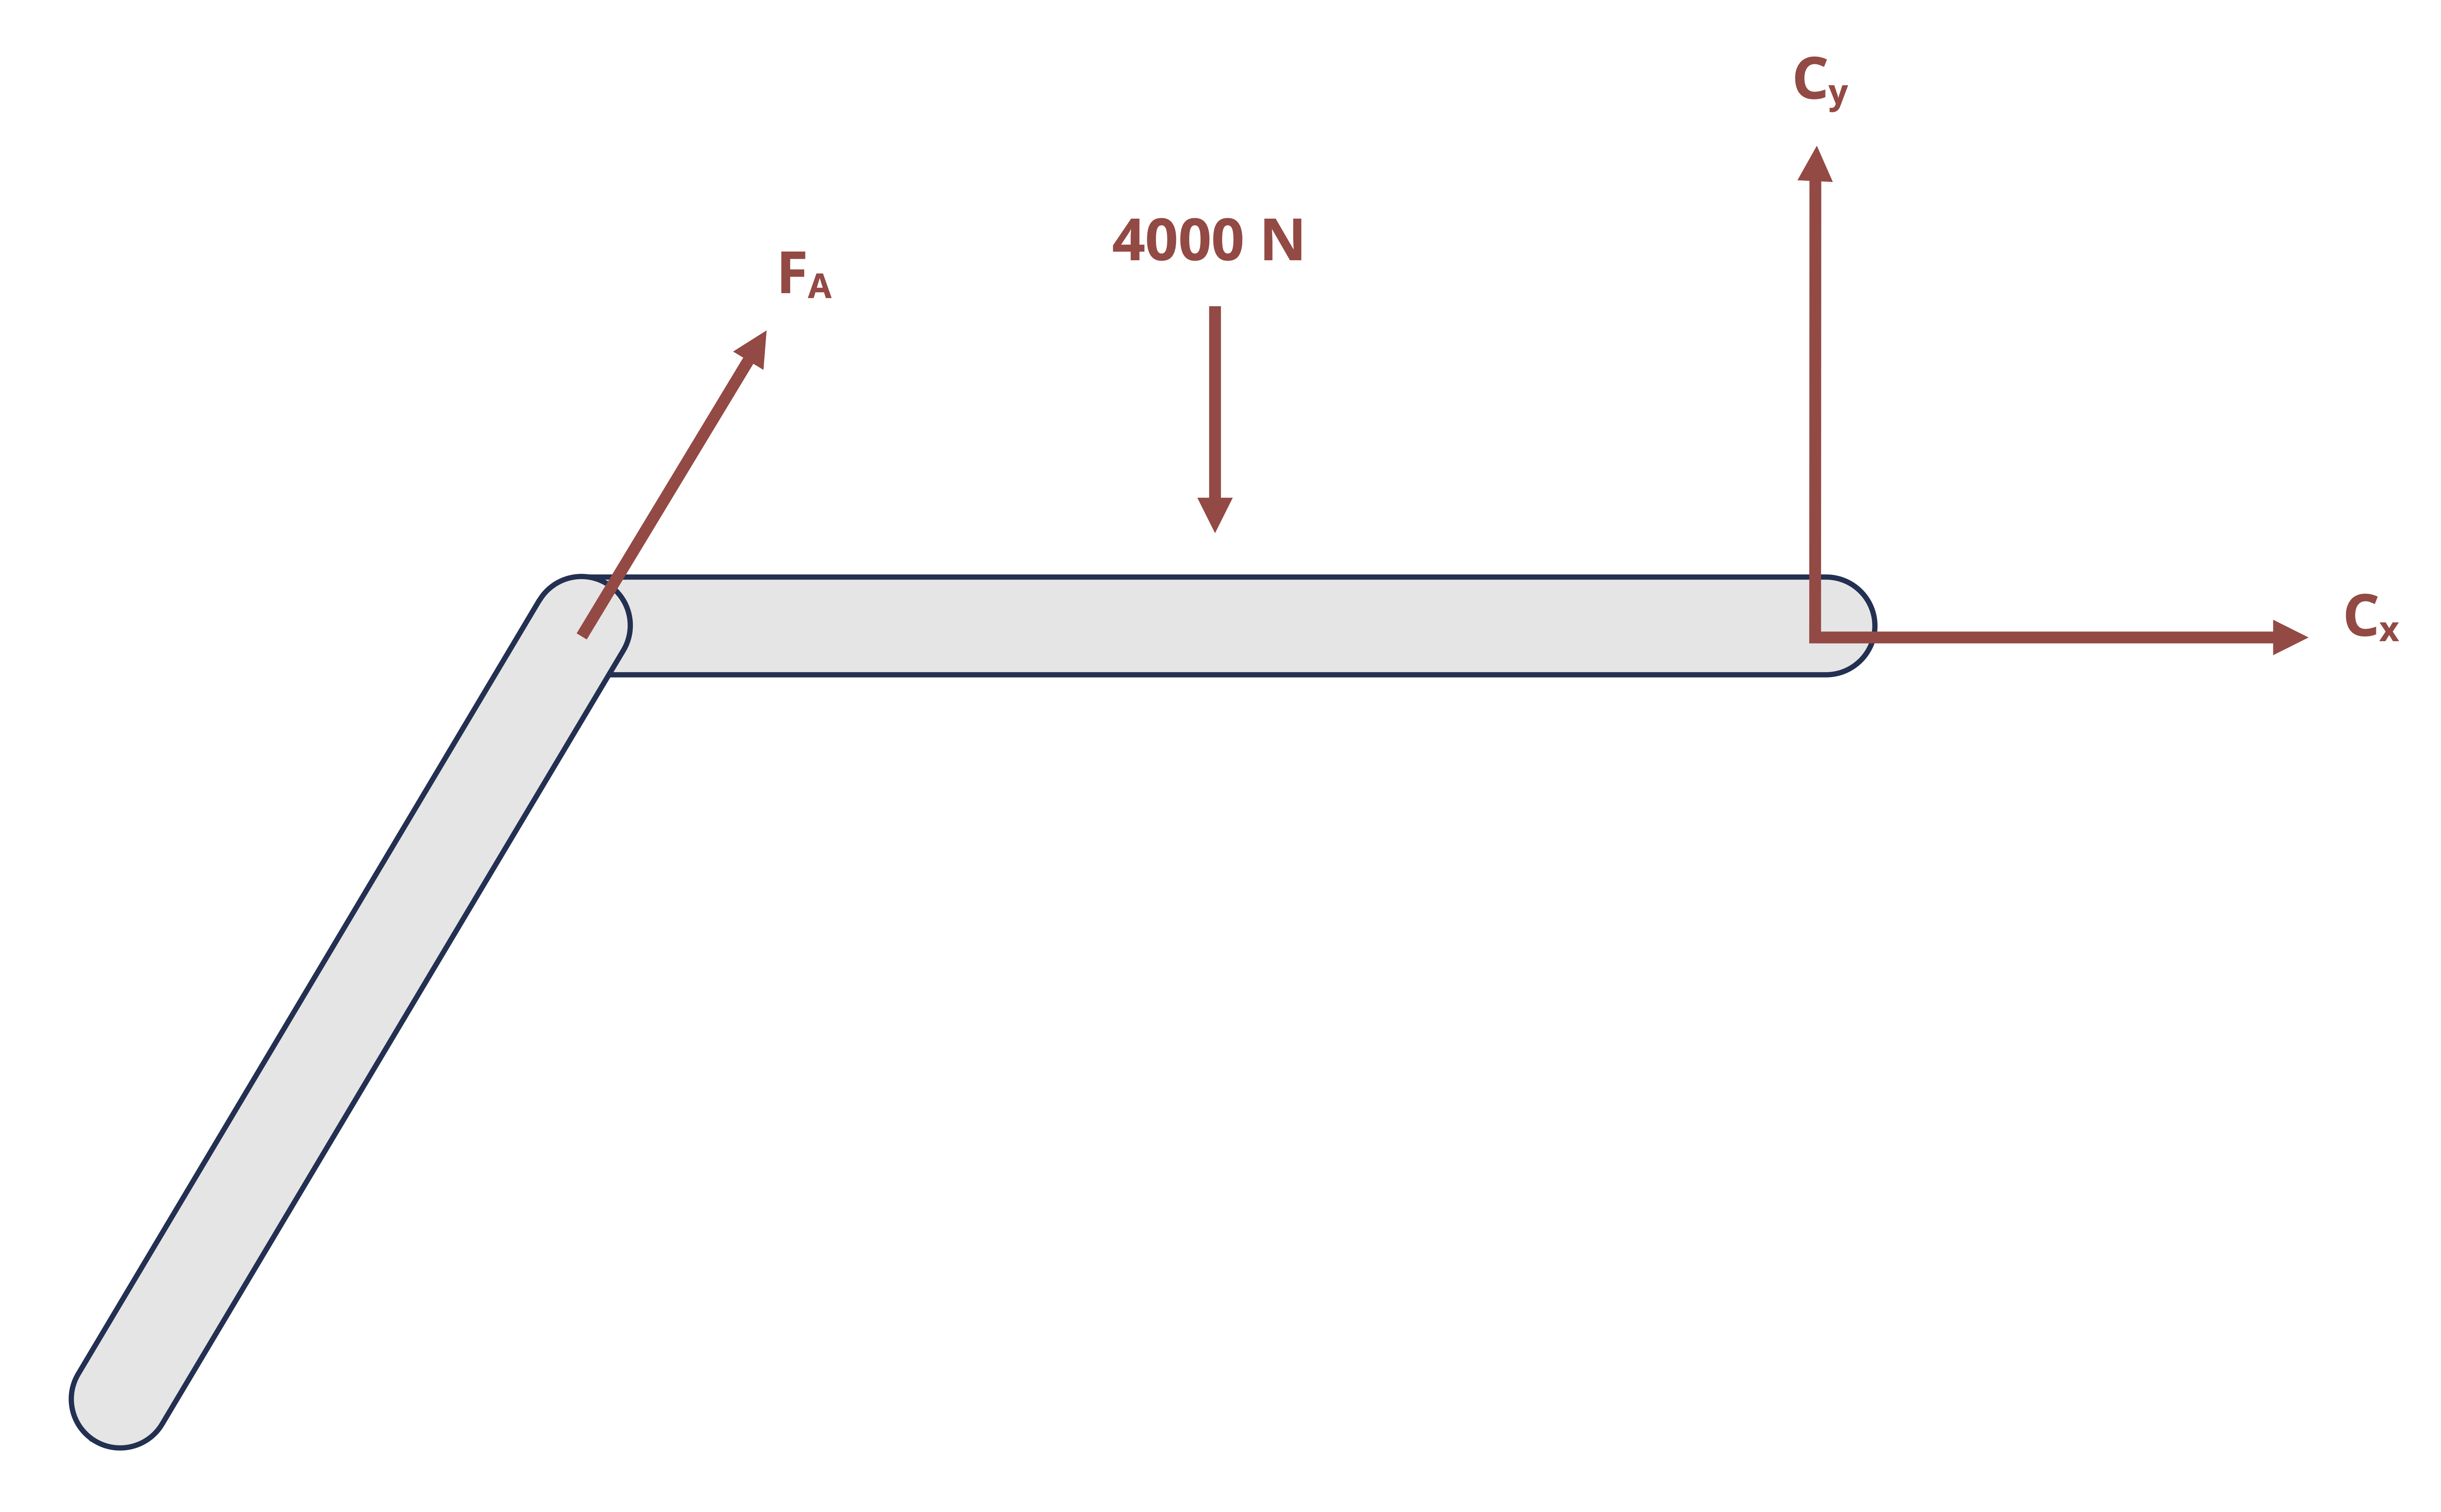
\includegraphics{images/clipboard-2163853552.png}\[
\sum M_C=-F_A \sin(50^\circ)*4{~m}+F_A \cos(50^\circ)*0+4,000{~N}*2{~m}=0
\]

This gives us the same result of \(F_A=2,611{~N}\) and the rest of the
problem proceeds the same way.

\begin{center}
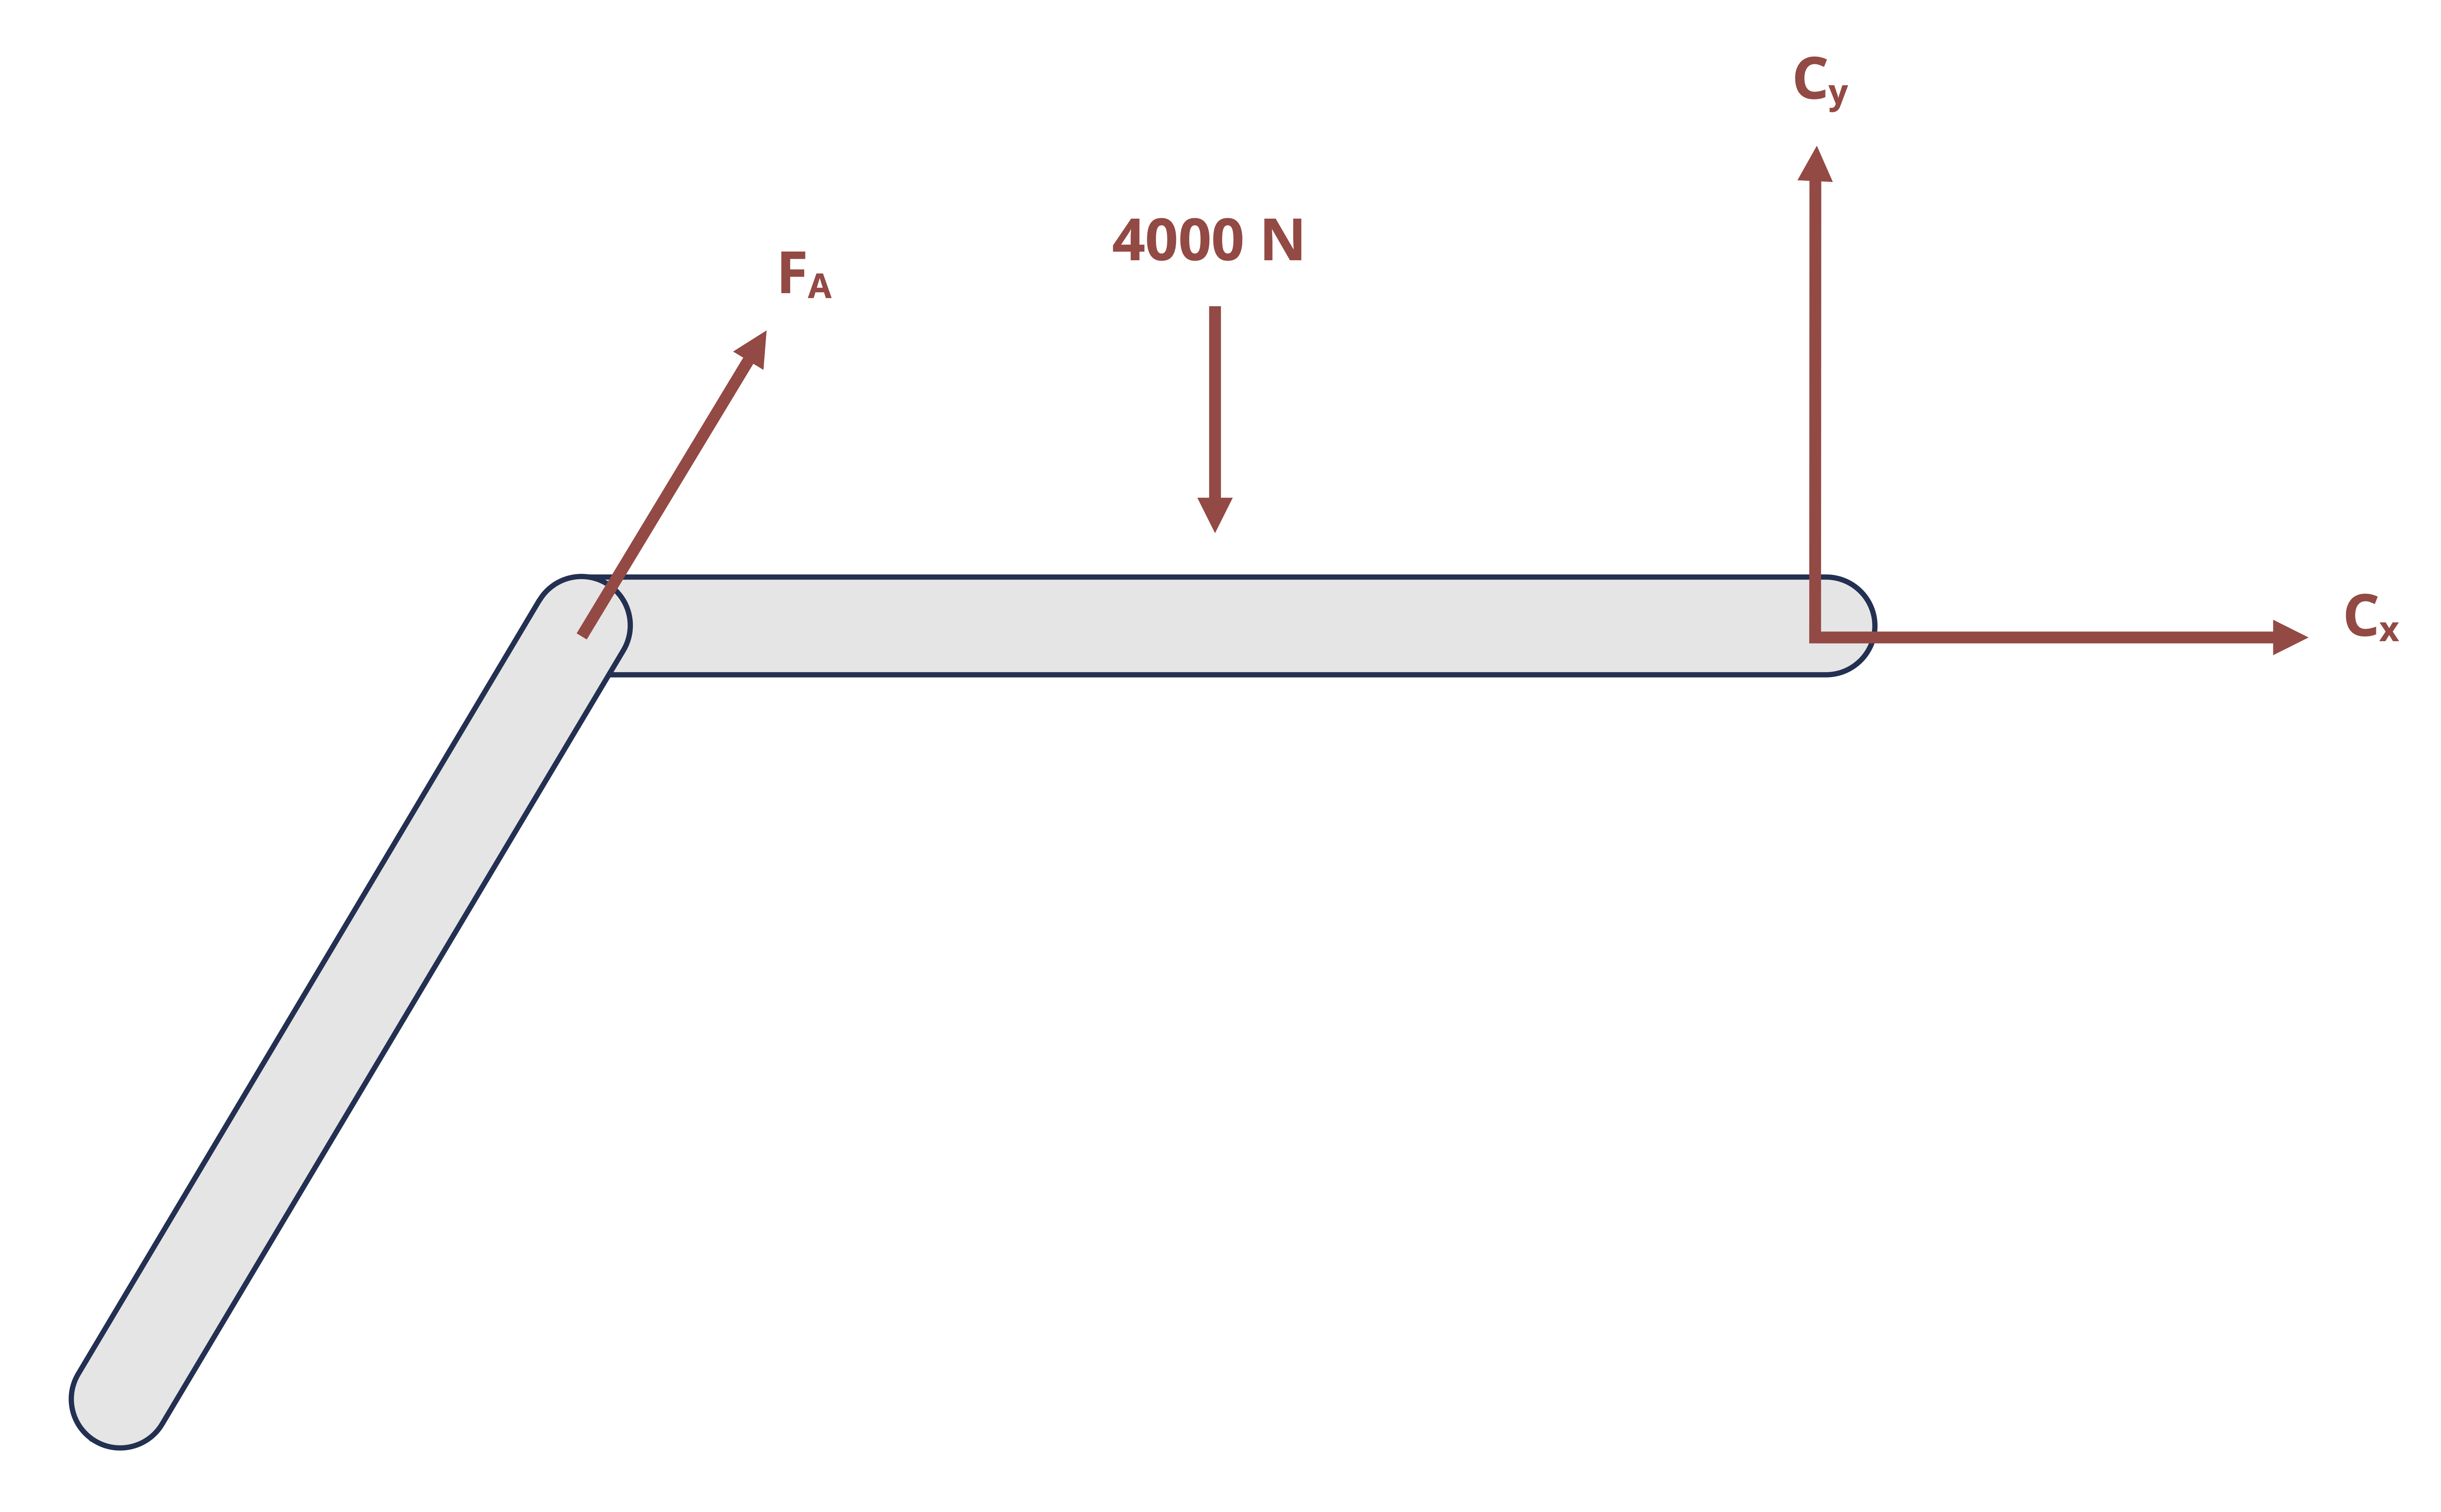
\includegraphics[width=4.05208in,height=\textheight]{images/Updated CH1 examples/example 1.2 part 4.png}
\end{center}

\textbf{Answer: F\textsubscript{A} = 1,155 N and F\textsubscript{C} =
1,155 N}

\end{tcolorbox}

\end{example}

\end{tcolorbox}

\section{Internal Reactions}\label{sec-1.2}

Click to expand

Internal reactions can refer to forces and moments at connection points
between members (such as a pin connecting multiple members of a frame,
machine, or truss), as well as to reactions at any point in a continuous
body (for example a point in the middle of a beam). These reactions are
the forces and/or moments necessary to hold a structure or a body
together and are ultimately the aspect of loading that is needed to
determine if and how a body will deform or even break.

\subsection{Internal reactions at a connection with two force
members}\label{internal-reactions-at-a-connection-with-two-force-members}

Pins that connect members can be represented on an FBD in the same way
as pins that connect the structure to external supports. That is, the
reaction would be drawn as the two components of the overall force.
However, the connected members would be considered as separate bodies,
as if the connecting pin were pulled out and the members separated. The
pin reactions would then be drawn on the FBD for each separated member.
Since the pin would exert equal and opposite forces on the connected
members, one needs to be careful to show the reaction forces in opposite
directions on the FBD's of those members. All three equilibrium
equations can be applied separately to each member so one could
theoretically solve for 3 times the number of unknowns as separate FBD's
drawn.

However, just as was discussed above, when one of the connected members
is a two-force member, the reaction at the pin will be known to follow a
line of action that goes through the points of application of the forces
on the two-force member. Example~\ref{exm-1.3} demonstrates these
concepts.

\begin{tcolorbox}[enhanced jigsaw, colback=white, colframe=quarto-callout-tip-color-frame, toptitle=1mm, arc=.35mm, bottomrule=.15mm, toprule=.15mm, opacitybacktitle=0.6, title={Example 1.3}, coltitle=black, breakable, colbacktitle=quarto-callout-tip-color!10!white, bottomtitle=1mm, titlerule=0mm, opacityback=0, leftrule=.75mm, left=2mm, rightrule=.15mm]

\begin{example}[]\protect\hypertarget{exm-1.3}{}\label{exm-1.3}

~

A plant hanger is secured to a wall with a pin and additionally
supported by a brace that is pin connected to the hanger at B and to the
wall at C. Determine the external reactions at A and C as well as the
reaction in the internal pin B.

\begin{center}
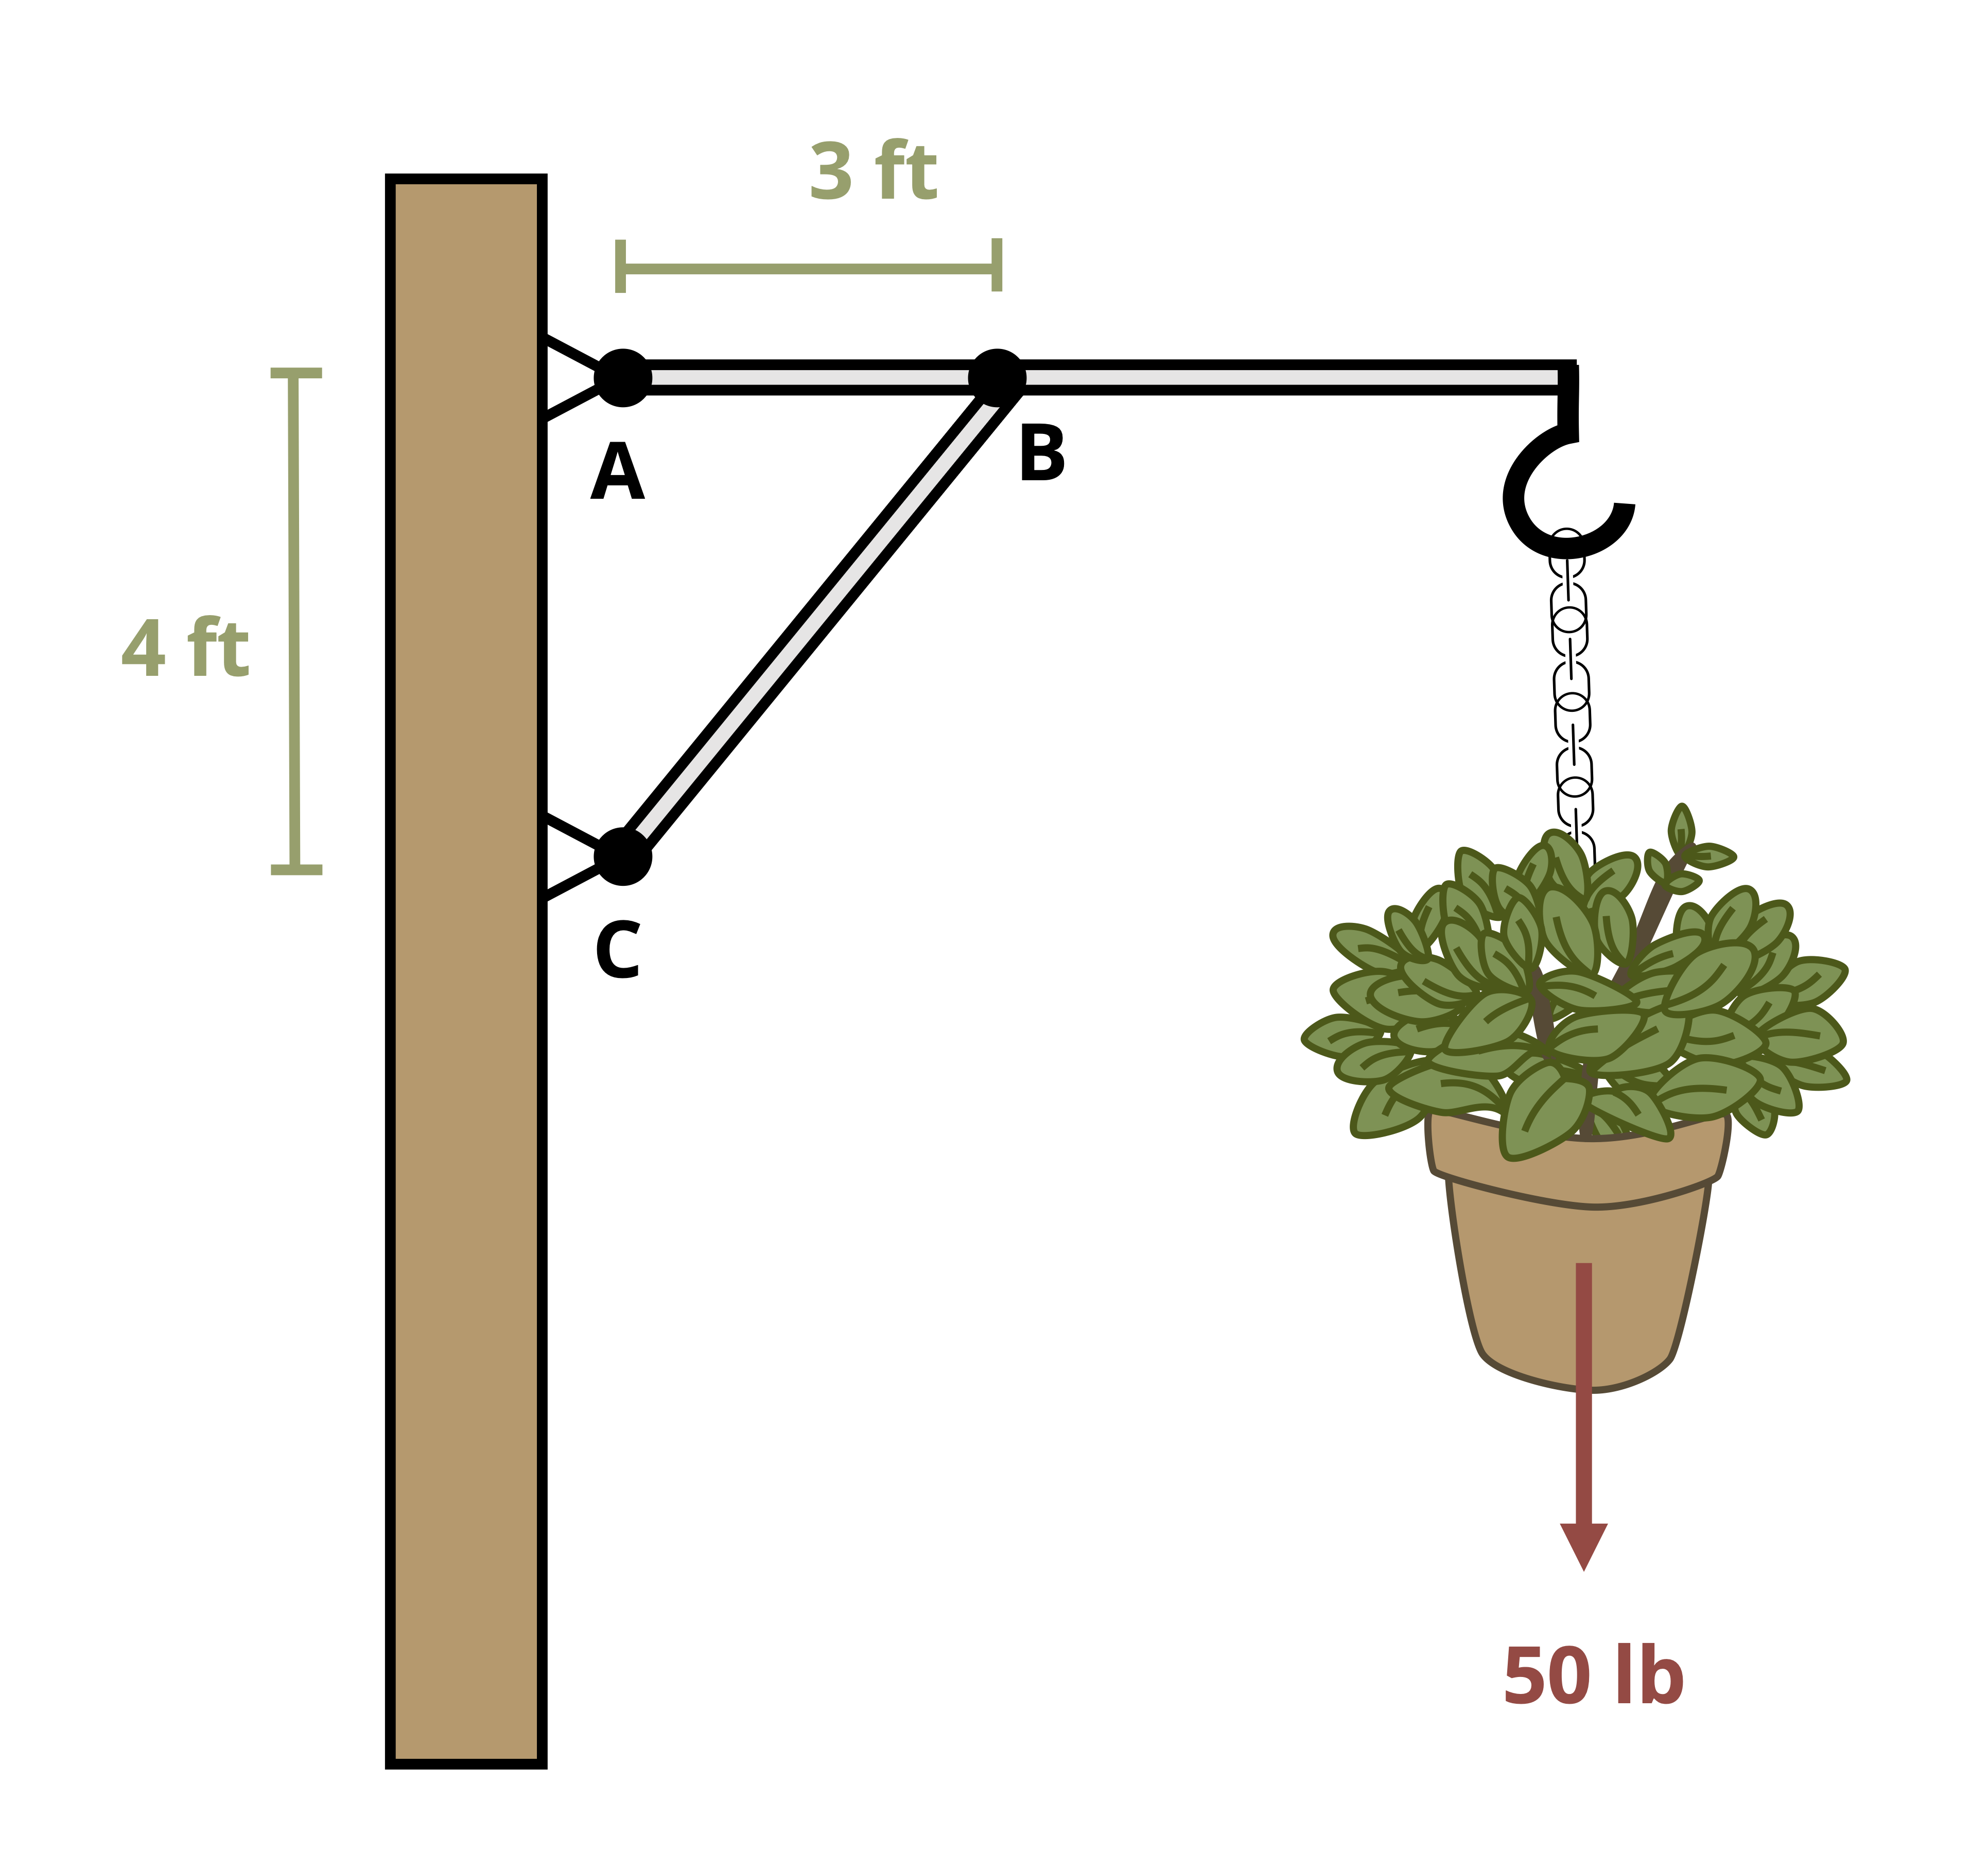
\includegraphics[width=3.28125in,height=\textheight]{images/CH1 PNGs/example 1.3 part 1.png}
\end{center}

\begin{tcolorbox}[enhanced jigsaw, colback=white, colframe=quarto-callout-tip-color-frame, toptitle=1mm, arc=.35mm, bottomrule=.15mm, toprule=.15mm, opacitybacktitle=0.6, title={Solution}, coltitle=black, breakable, colbacktitle=quarto-callout-tip-color!10!white, bottomtitle=1mm, titlerule=0mm, opacityback=0, leftrule=.75mm, left=2mm, rightrule=.15mm]

If we do not notice that BC is a two-force member, we would approach the
problem by separating the brace from the hanger and drawing an FBD of
each part separately. Notice that B\textsubscript{x} and
B\textsubscript{y} are drawn in opposite directions in the two different
diagrams since the pin will exert an equal and opposite force on each
bar.

\begin{center}
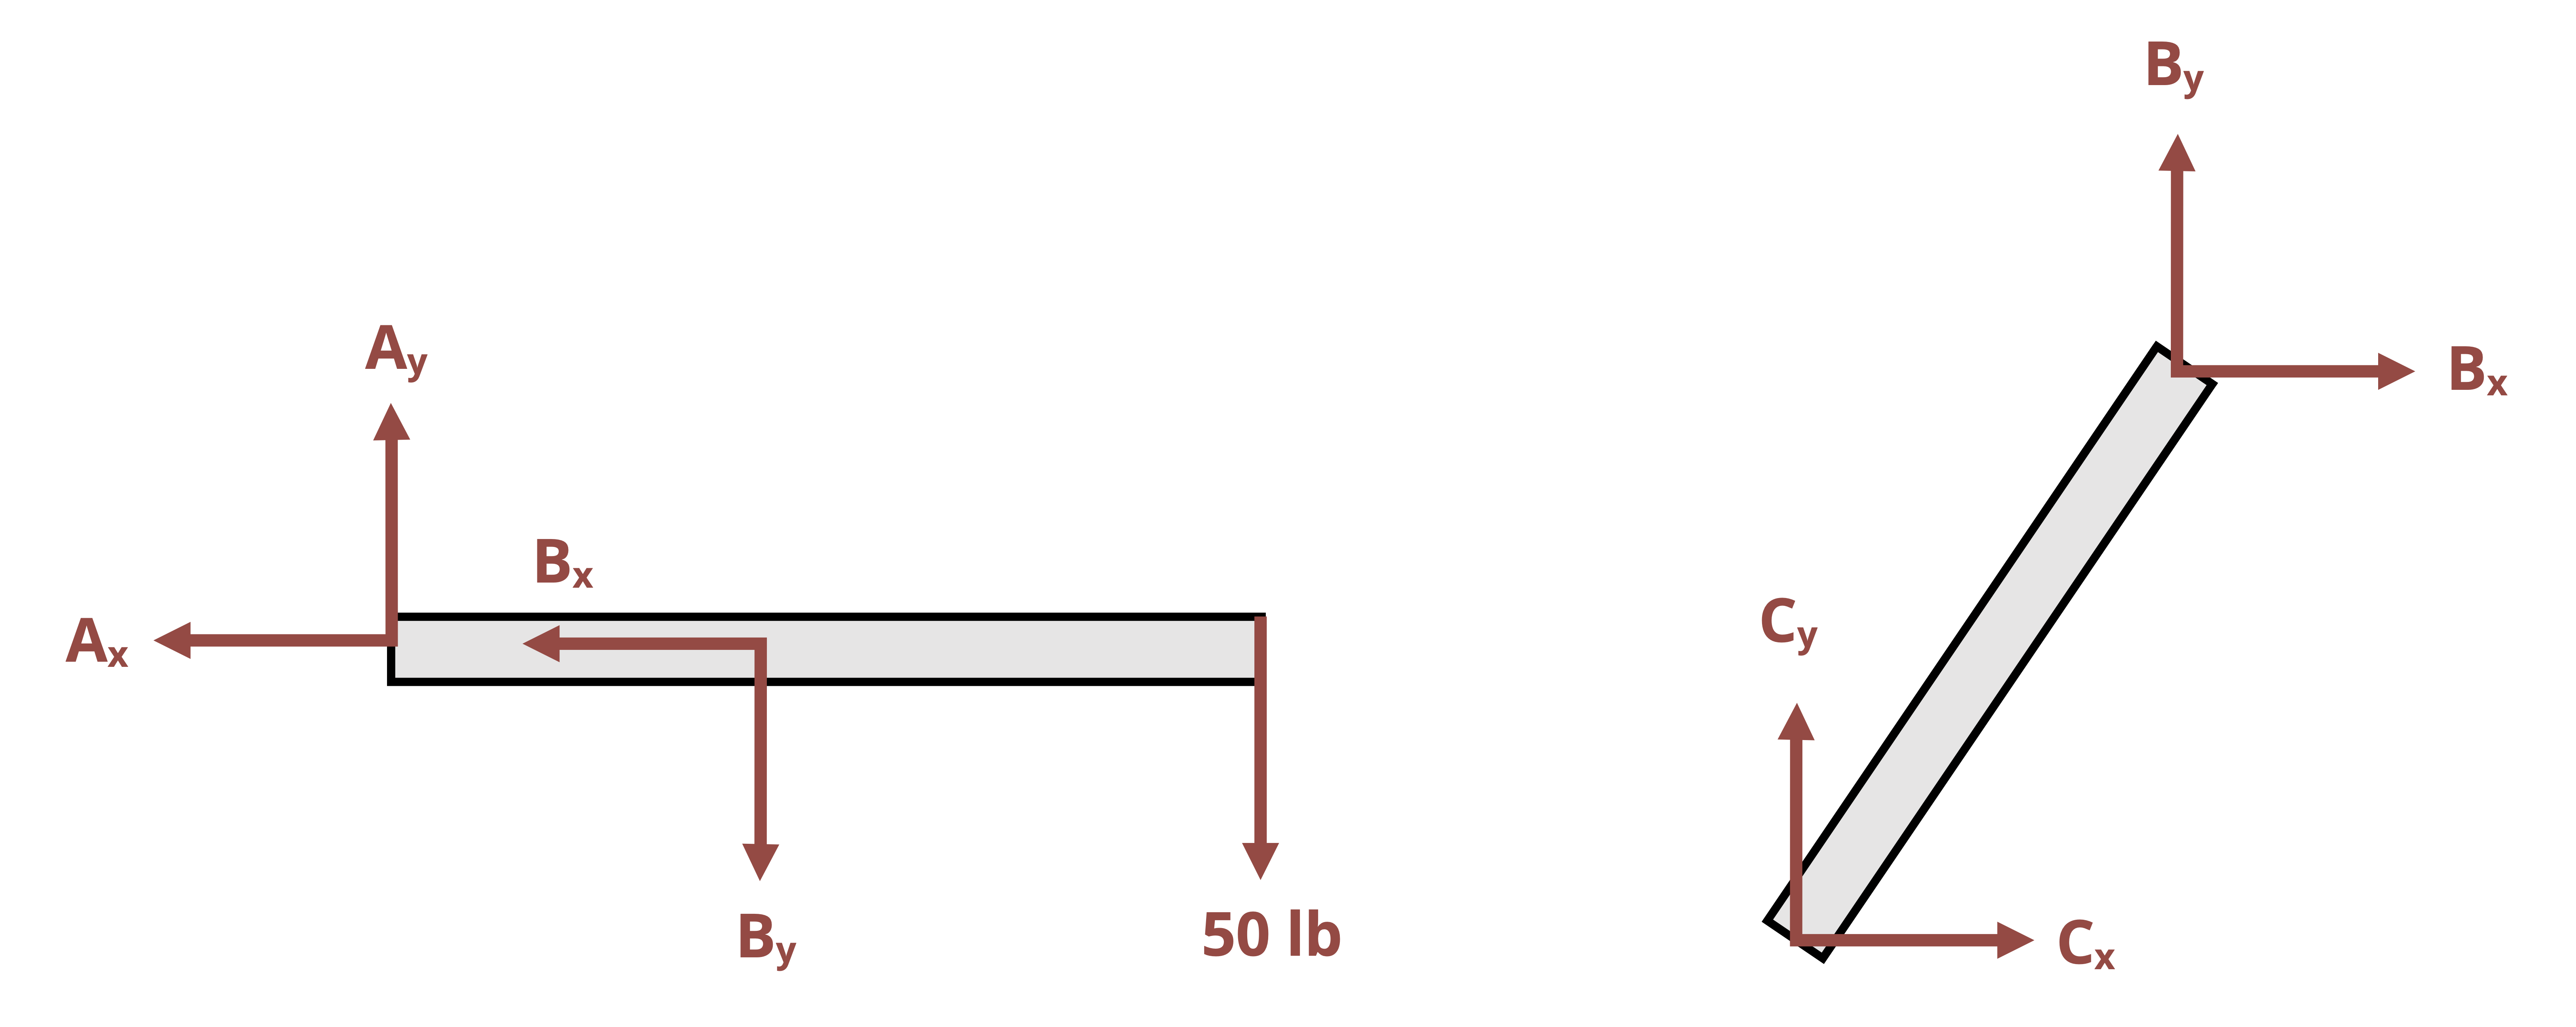
\includegraphics[width=5.86458in,height=\textheight]{images/CH1 PNGs/example 1.3 part 2.png}
\end{center}

There are now 6 unknowns and 6 equilibrium equations (3 equations per
body) available to use per bar, so the problem is technically solvable.
However, since BC is a two force member (there is a pin force at B and a
pin force at C but no other forces at any other point on the bar), it
can be taken as known that the reaction force at B follows a line of
action that goes through B and C. We can also conclude that the force in
pin C is equal to the force in pin B. The FBD of bar AB can be redrawn:

\begin{center}
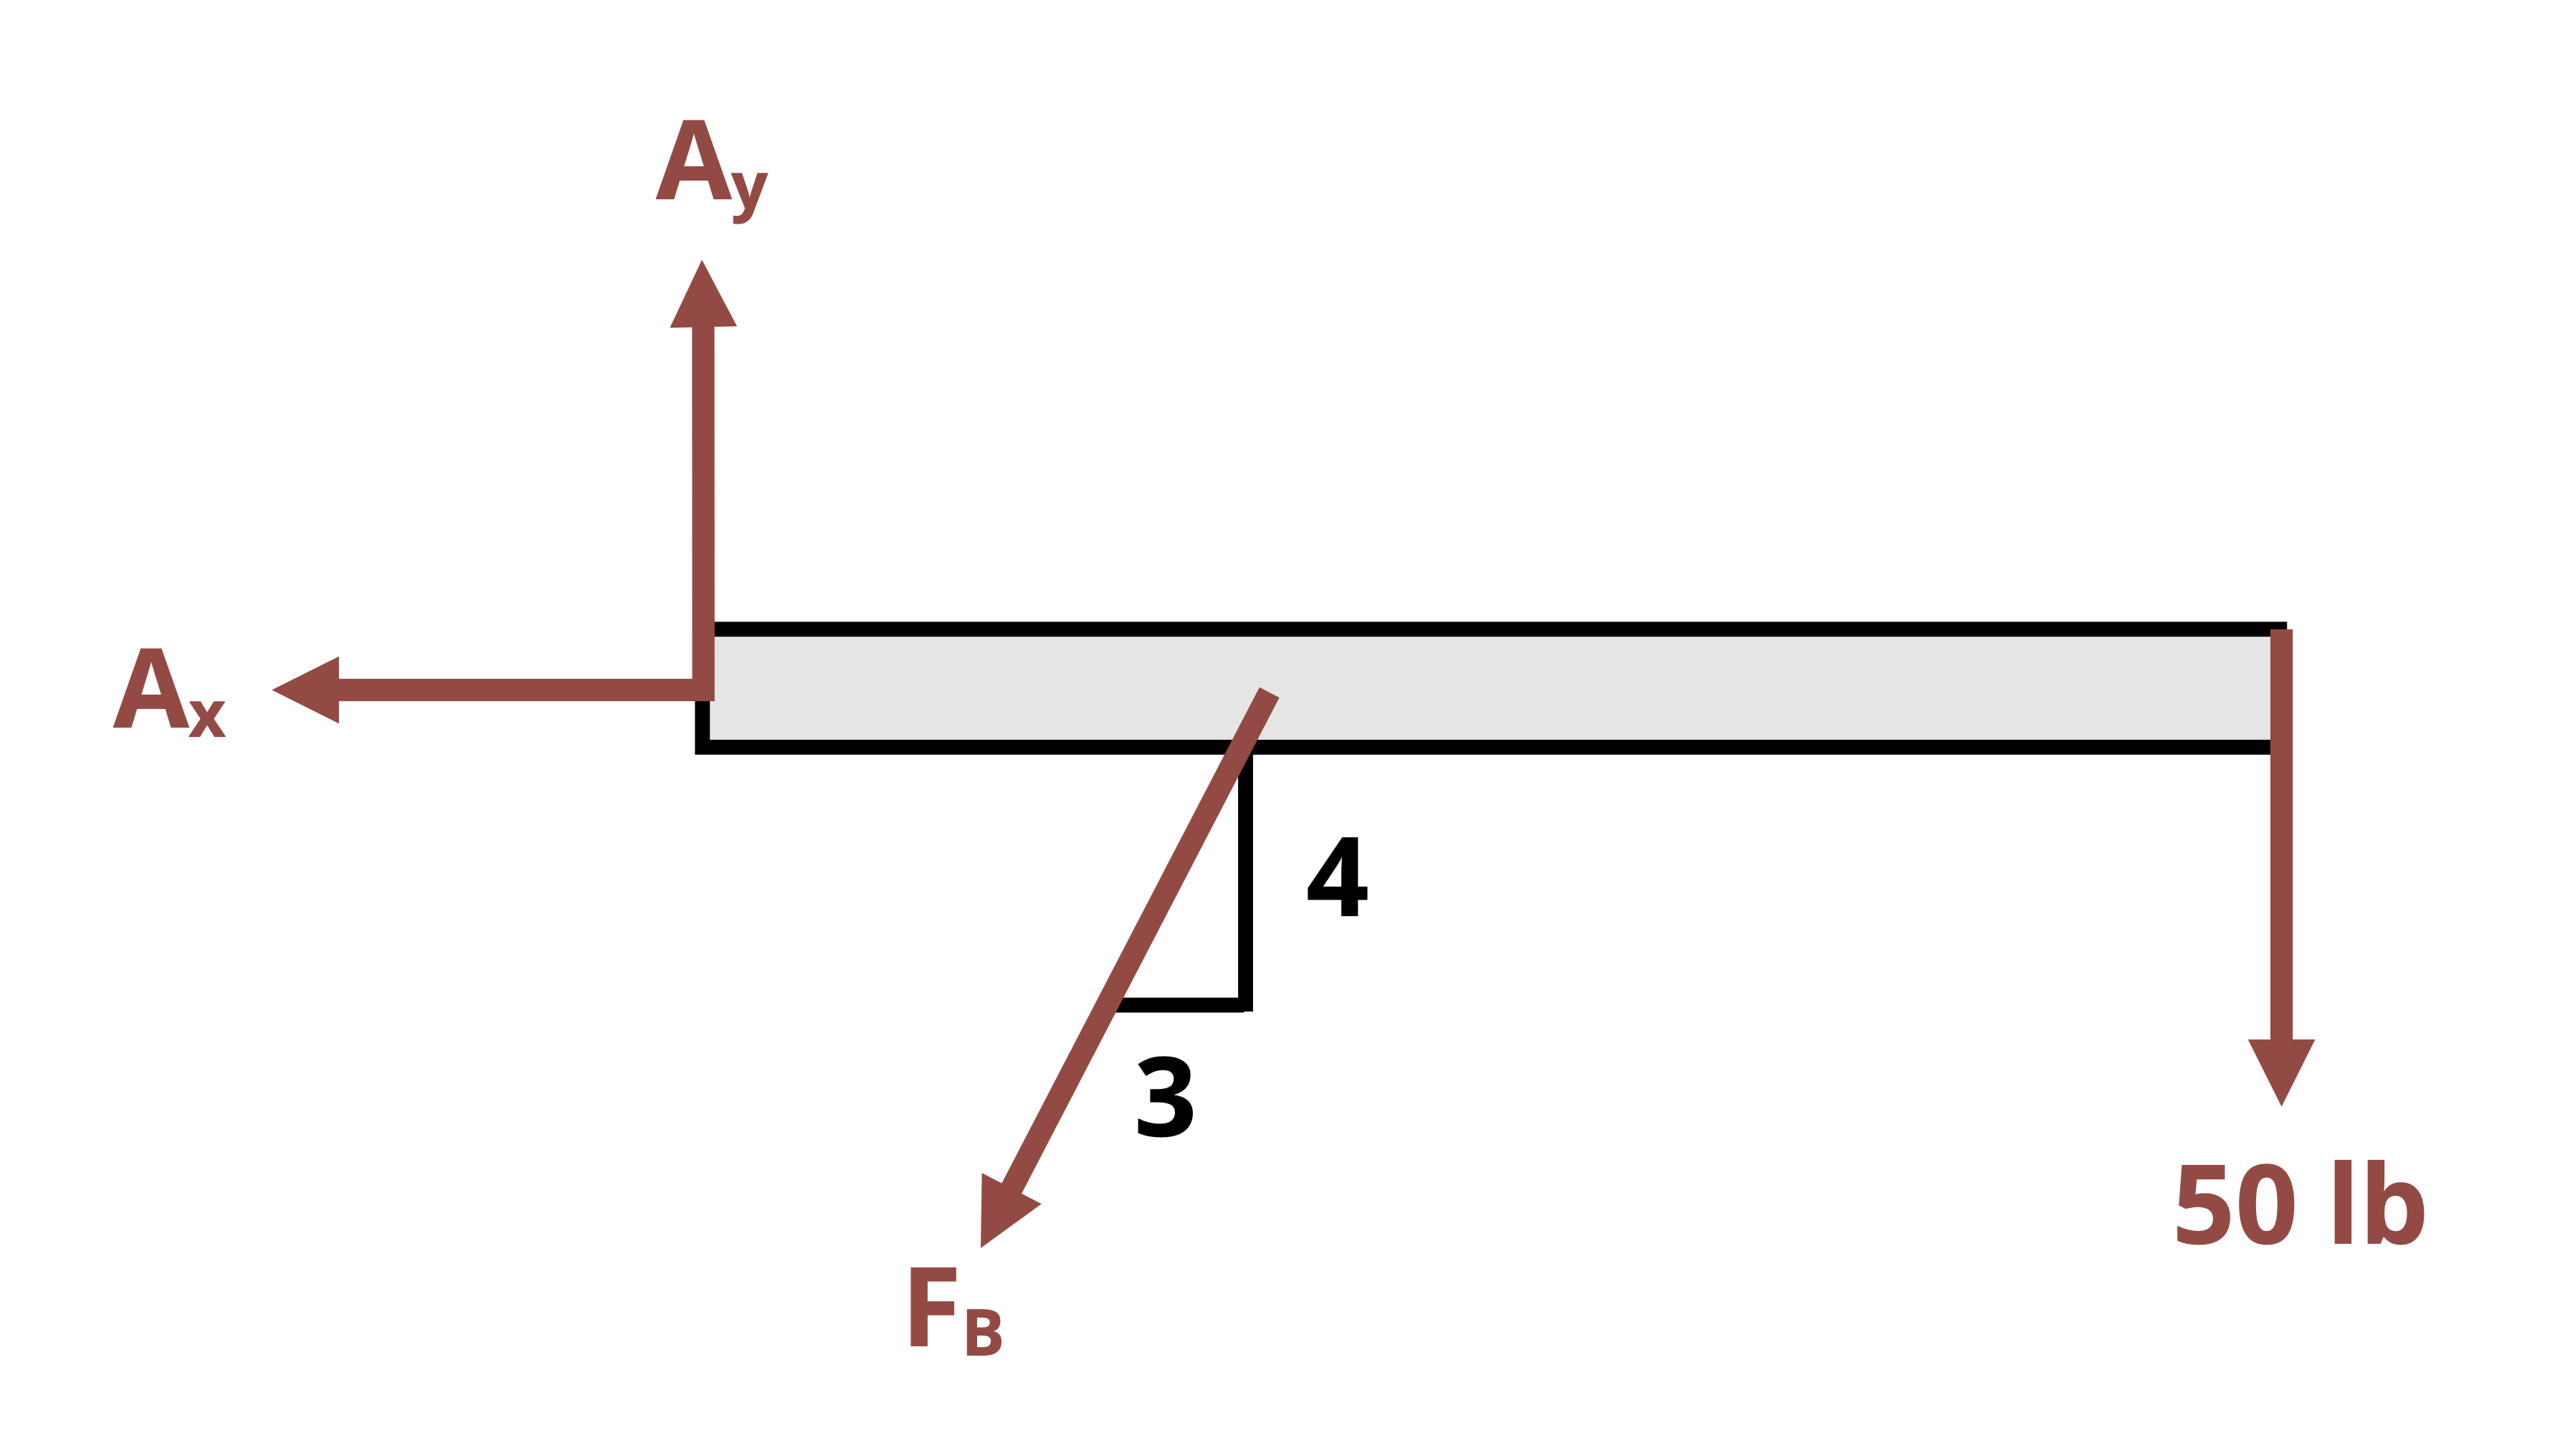
\includegraphics[width=3.1875in,height=\textheight]{images/CH1 PNGs/example 1.3 part 3.png}
\end{center}

With the components B\textsubscript{x} and B\textsubscript{y} replaced
with the resultant force F\textsubscript{B} with known direction, the
number of unknowns on bar AB is reduced to 3. These unknowns can be
solved for using the equilibrium equations:

\[
\begin{aligned}
& \sum M_A=F_B\left(\frac{4}{5}\right)*3{~ft}-50{~lb}*7{~ft}=0 \\
& \sum F_x=-A_x+F_B\left(\frac{3}{5}\right)=0 \\
& \sum F_y=A_y+F_B\left(\frac{4}{5}\right)-50{~lb}=0
\end{aligned}
\]

Solving the equations (1)-(3) yields F\textsubscript{B} = 145.8 lb,
A\textsubscript{x} = 87.5 lb, and A\textsubscript{y} = -66.7 lb.
Therefore, the pin force in pin B is 145.8 lb and the pin force in A is
\(\mathrm{A}=\sqrt{A_x^2+A_y^2}=110{~lb}\). Since BC is a two-force
member, F\textsubscript{C} = F\textsubscript{B}.

\textbf{Answer: F\textsubscript{A} = 110 lb, F\textsubscript{B} =
F\textsubscript{C} = 146.8 lb}

\end{tcolorbox}

\end{example}

\end{tcolorbox}

\subsection{Internal reactions in truss
structures}\label{internal-reactions-in-truss-structures}

Truss structures are made up of only two force members. The two main
methods of determining internal reactions in planar (2D) truss
structures are Method of Joints and Method of Sections. In using Method
of Joints, an FBD is drawn of the connecting pins (joints) within the
truss. Since all the members connected at any given pin will be
two-force members, the reactions can be drawn in known directions.
However, since the forces all pass through the same point on the body,
the moment equilibrium equation is not useful, so only the forces
equilibrium equations can be used for each joint. This means that only
two unknowns can be solved for at each joint. This method is most useful
when the forces of all the truss members are sought or if the only
forces sought are attached to a joint with only two members.

To use Method of Sections, a cut is made through the truss structure and
analysis is based on the FBD of the intact part of the structure that is
to the left of the cut or the intact part of the structure to the right
of the cut. The FBD of either given side will show the applied forces
and the reaction forces from the members that were cut through. These
reactions will be equal in magnitude but opposite in direction between
the two sides of the cut. The side to examine is usually based on which
one will not require having to find external reactions (if there is a
free end to the truss) and/or which one is least complicated to deal
with in terms of geometry or applied loads. All three equilibrium
equations can generally be effectively applied with Method of Sections,
so three unknowns can be solved for with any given cut.

Example~\ref{exm-1.4} demonstrates the use of both Method of Joints and
Method of Sections to solve for forces in truss members.

\begin{tcolorbox}[enhanced jigsaw, colback=white, colframe=quarto-callout-tip-color-frame, toptitle=1mm, arc=.35mm, bottomrule=.15mm, toprule=.15mm, opacitybacktitle=0.6, title={Example 1.4}, coltitle=black, breakable, colbacktitle=quarto-callout-tip-color!10!white, bottomtitle=1mm, titlerule=0mm, opacityback=0, leftrule=.75mm, left=2mm, rightrule=.15mm]

\begin{example}[]\protect\hypertarget{exm-1.4}{}\label{exm-1.4}

~

Determine the forces in members ED and EF. Let P\textsubscript{1} = 8 kN
and P\textsubscript{2} = 12 kN.

\begin{center}
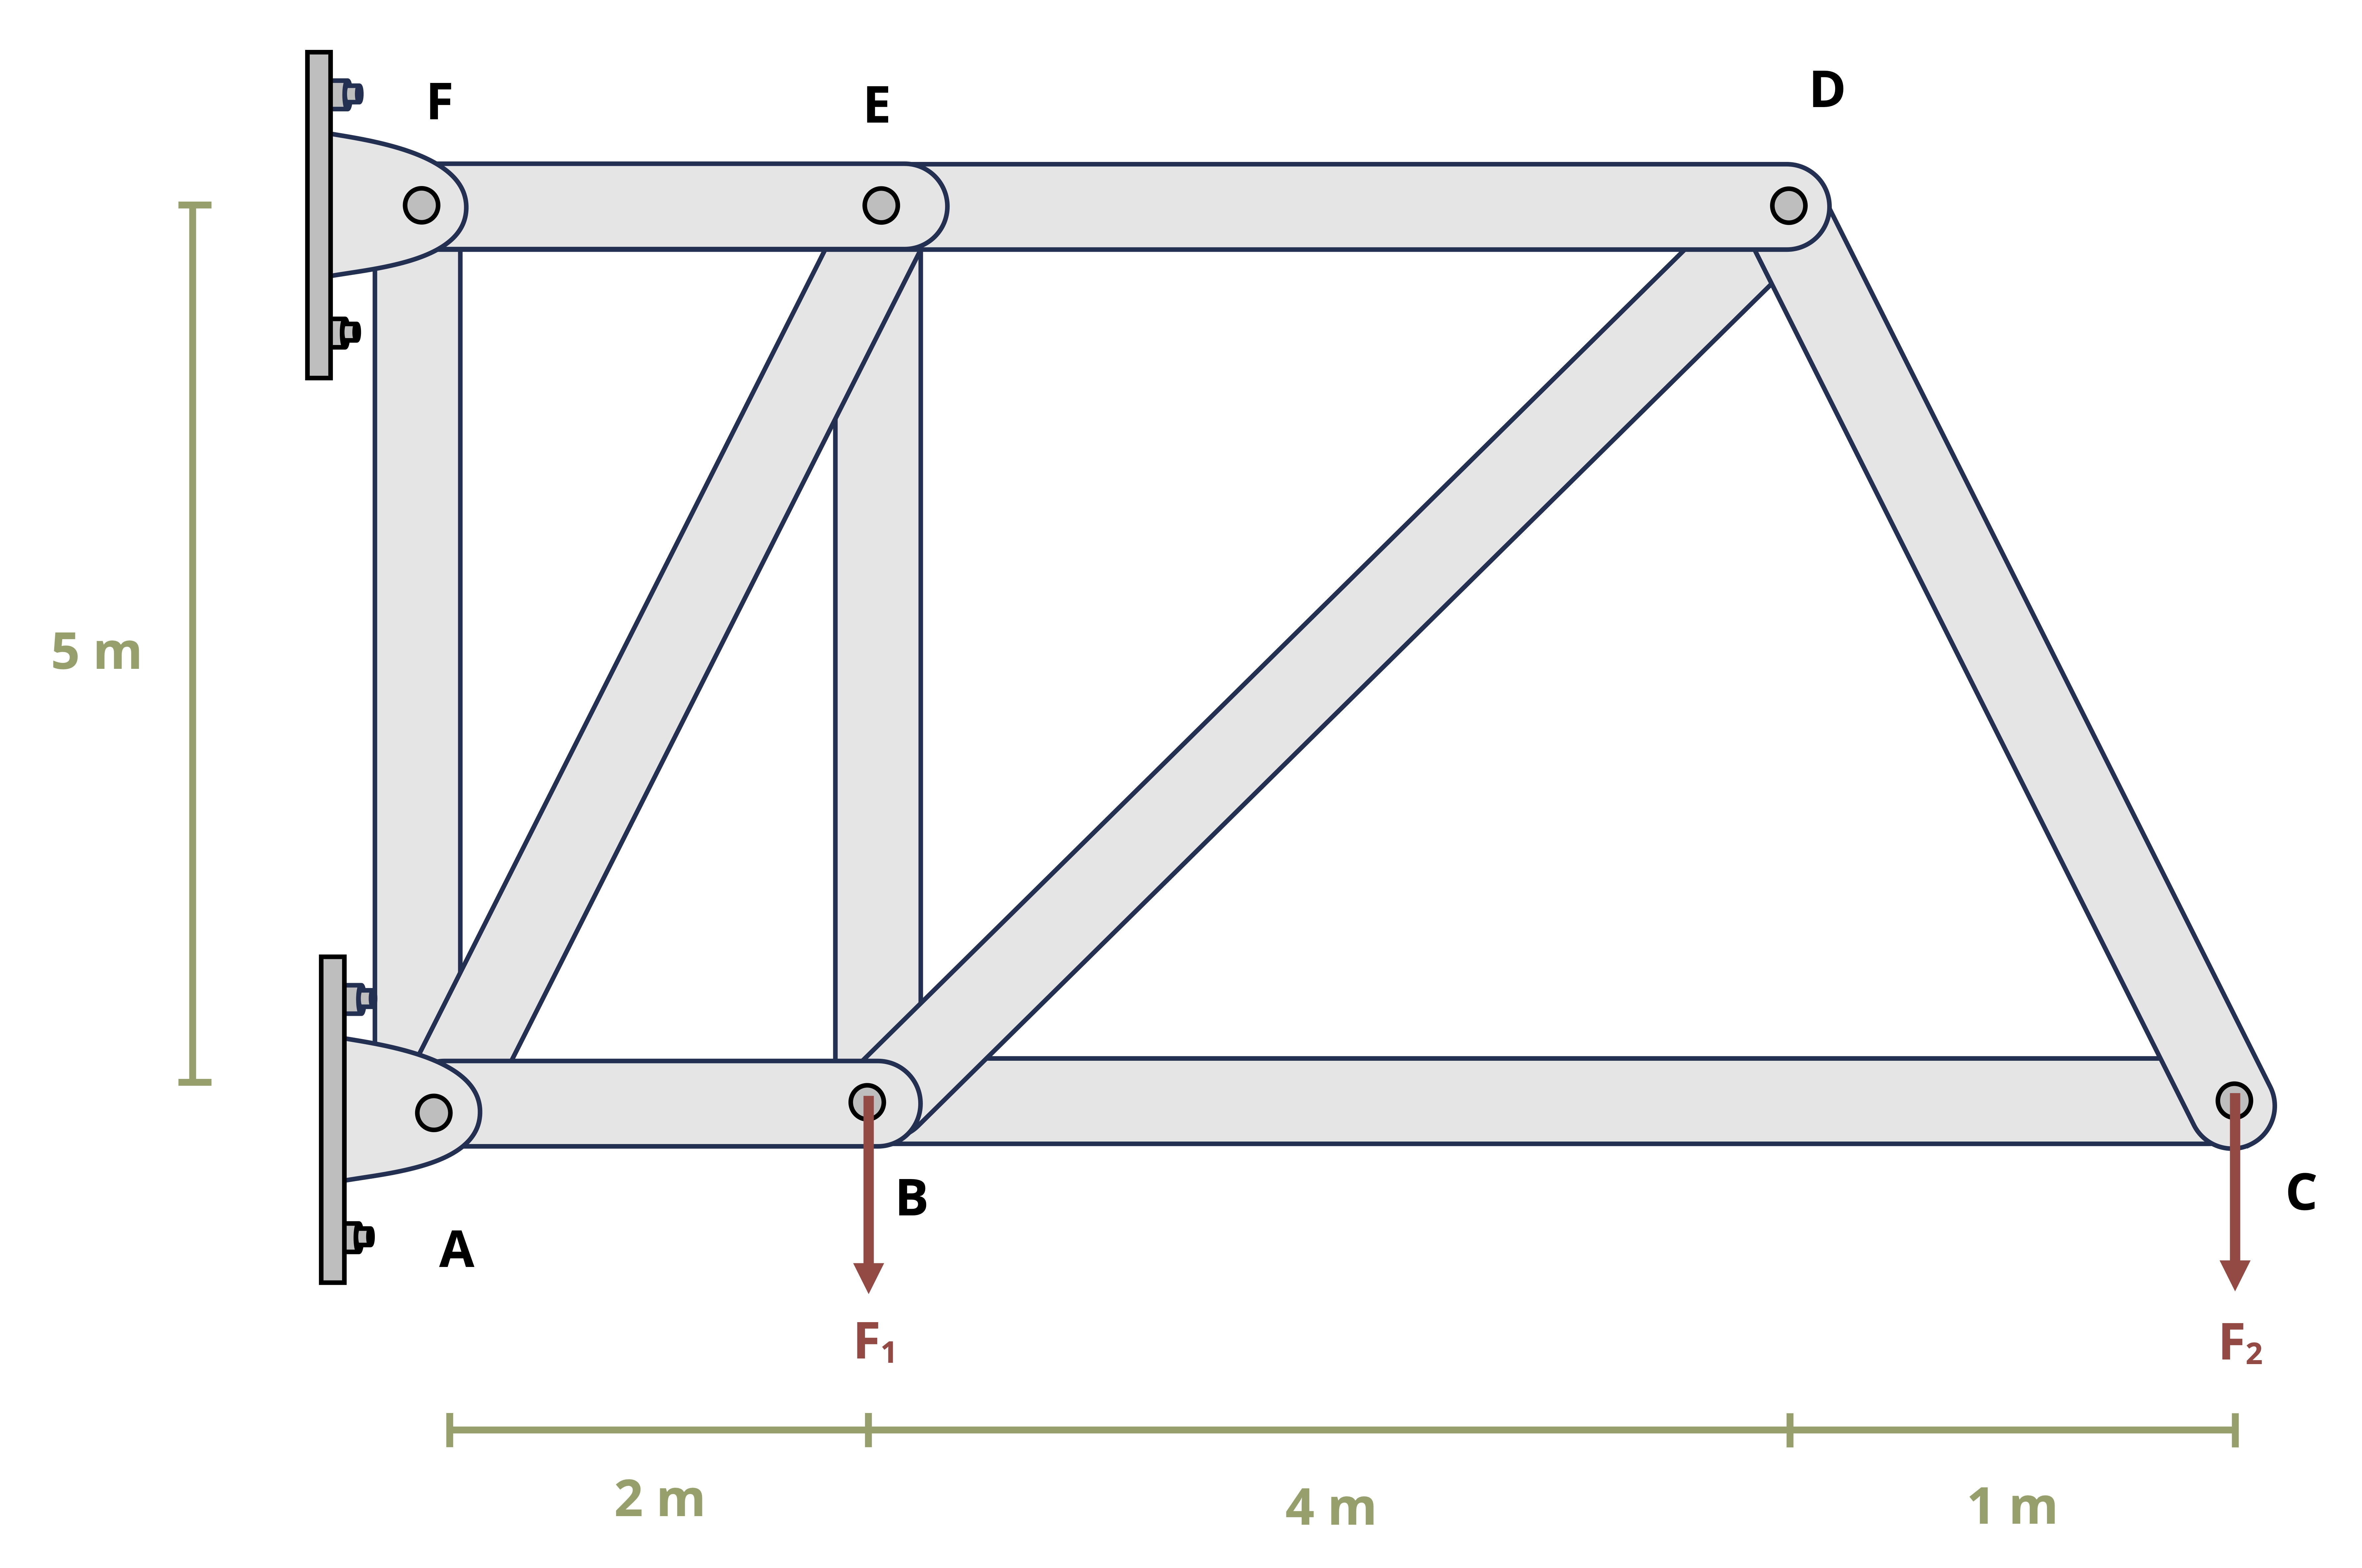
\includegraphics[width=3.96875in,height=\textheight]{images/Updated CH1 examples/example 1.4 part 1.png}
\end{center}

\begin{tcolorbox}[enhanced jigsaw, colback=white, colframe=quarto-callout-tip-color-frame, toptitle=1mm, arc=.35mm, bottomrule=.15mm, toprule=.15mm, opacitybacktitle=0.6, title={Solution - Method of Joints}, coltitle=black, breakable, colbacktitle=quarto-callout-tip-color!10!white, bottomtitle=1mm, titlerule=0mm, opacityback=0, leftrule=.75mm, left=2mm, rightrule=.15mm]

With method of joints, we should always work with a joint that has no
more than two unknown forces acting on it. These unknown forces come
from either members attached to the joint or from external support
reactions. Joint C is a good place to start here, as there are only two
unknown forces: BC and CD.

\textbf{FBD Joint C}

\begin{center}
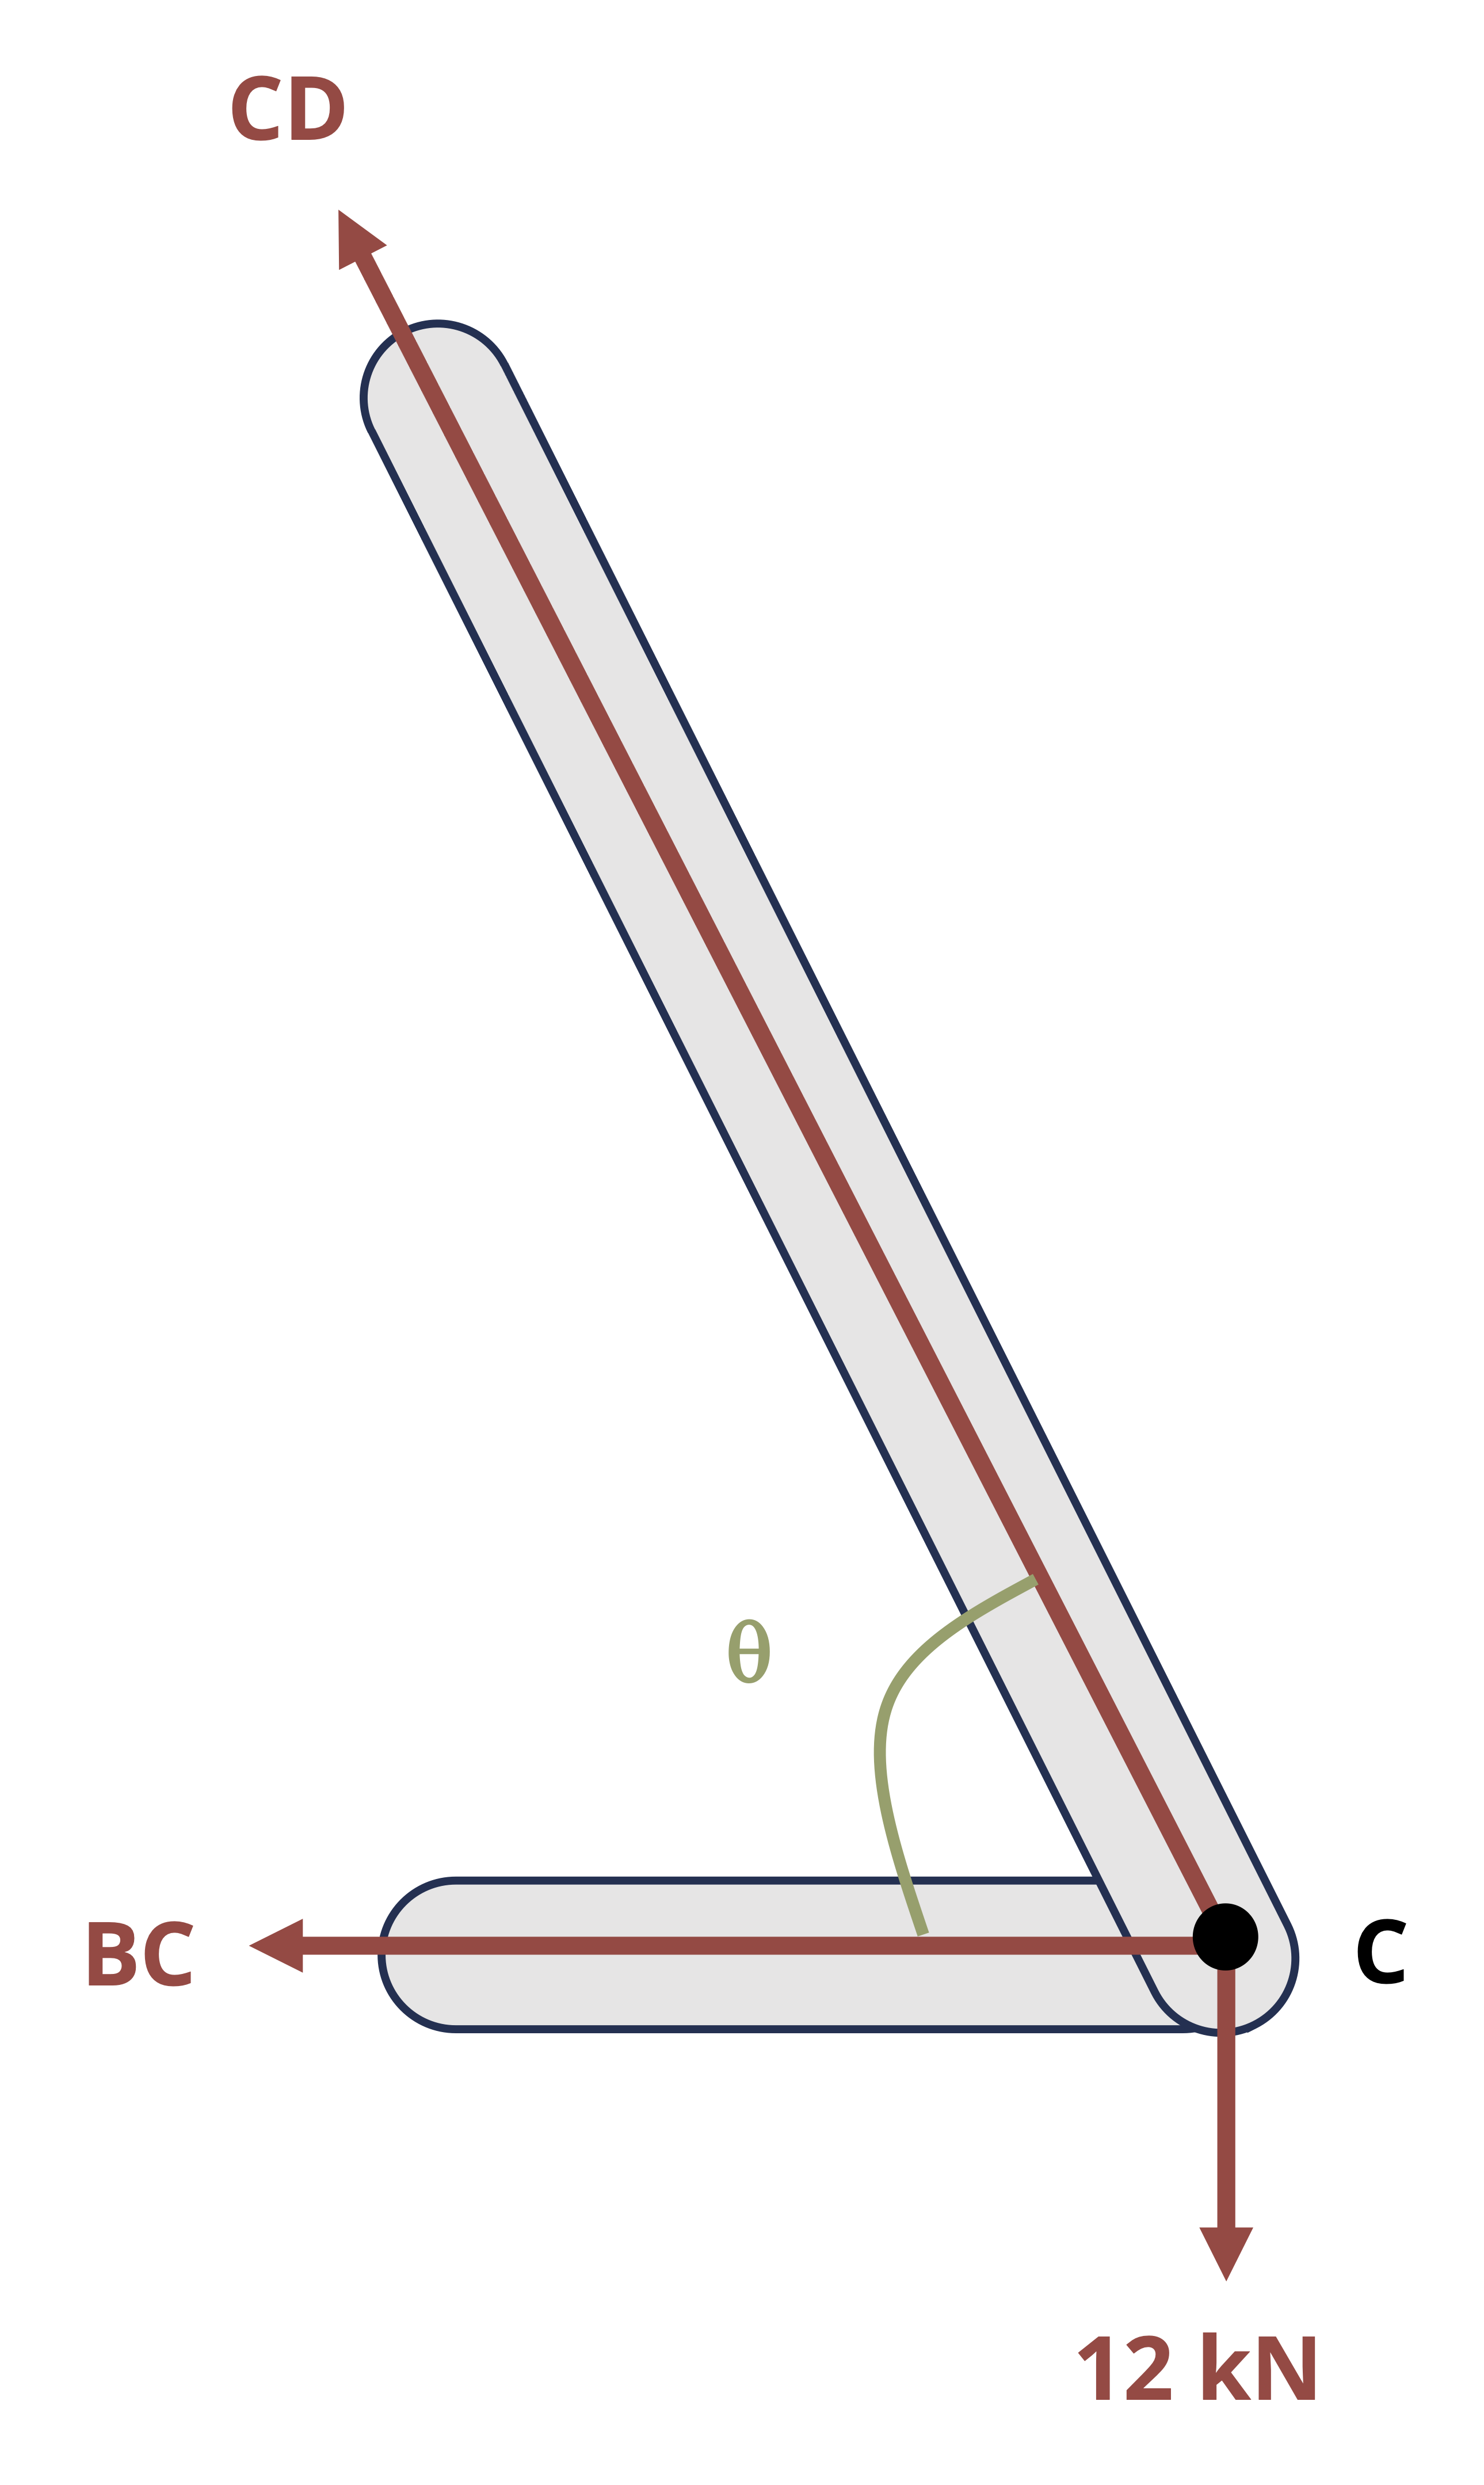
\includegraphics[width=2.32292in,height=\textheight]{images/Updated CH1 examples/example 1.4 part 2.png}
\end{center}

Angle Θ can be found by setting up a right angle triangle at C with a
base of 1 m and a height of 5 m. Once this angle is known, we can use
equilibrium equations to find the forces in members BC and CD.~

\[
\theta=\tan ^{-1}\left(\frac{5}{1}\right)=78.7^{\circ} \\
\\
\begin{aligned}
&\sum F_y=C D \sin \left(78.7^{\circ}\right)-12=0 \quad\rightarrow\quad C D=12.2{~kN} \\
&\sum F_x=-B C-C D \cos \left(78.7^{\circ}\right)=0 \quad\rightarrow\quad B D=-15.3{~kN}
\end{aligned}
\]

Since the forces are shown to be tensile in the FBD (the forces are
pointed away from the joint), the negative answer indicates that force
BD is actually compressive.

Now that force CD is known to be 12.2 kN in tension, there are two
remaining unknowns at joint D: BD and DE.

\textbf{FBD Joint D}

\begin{center}
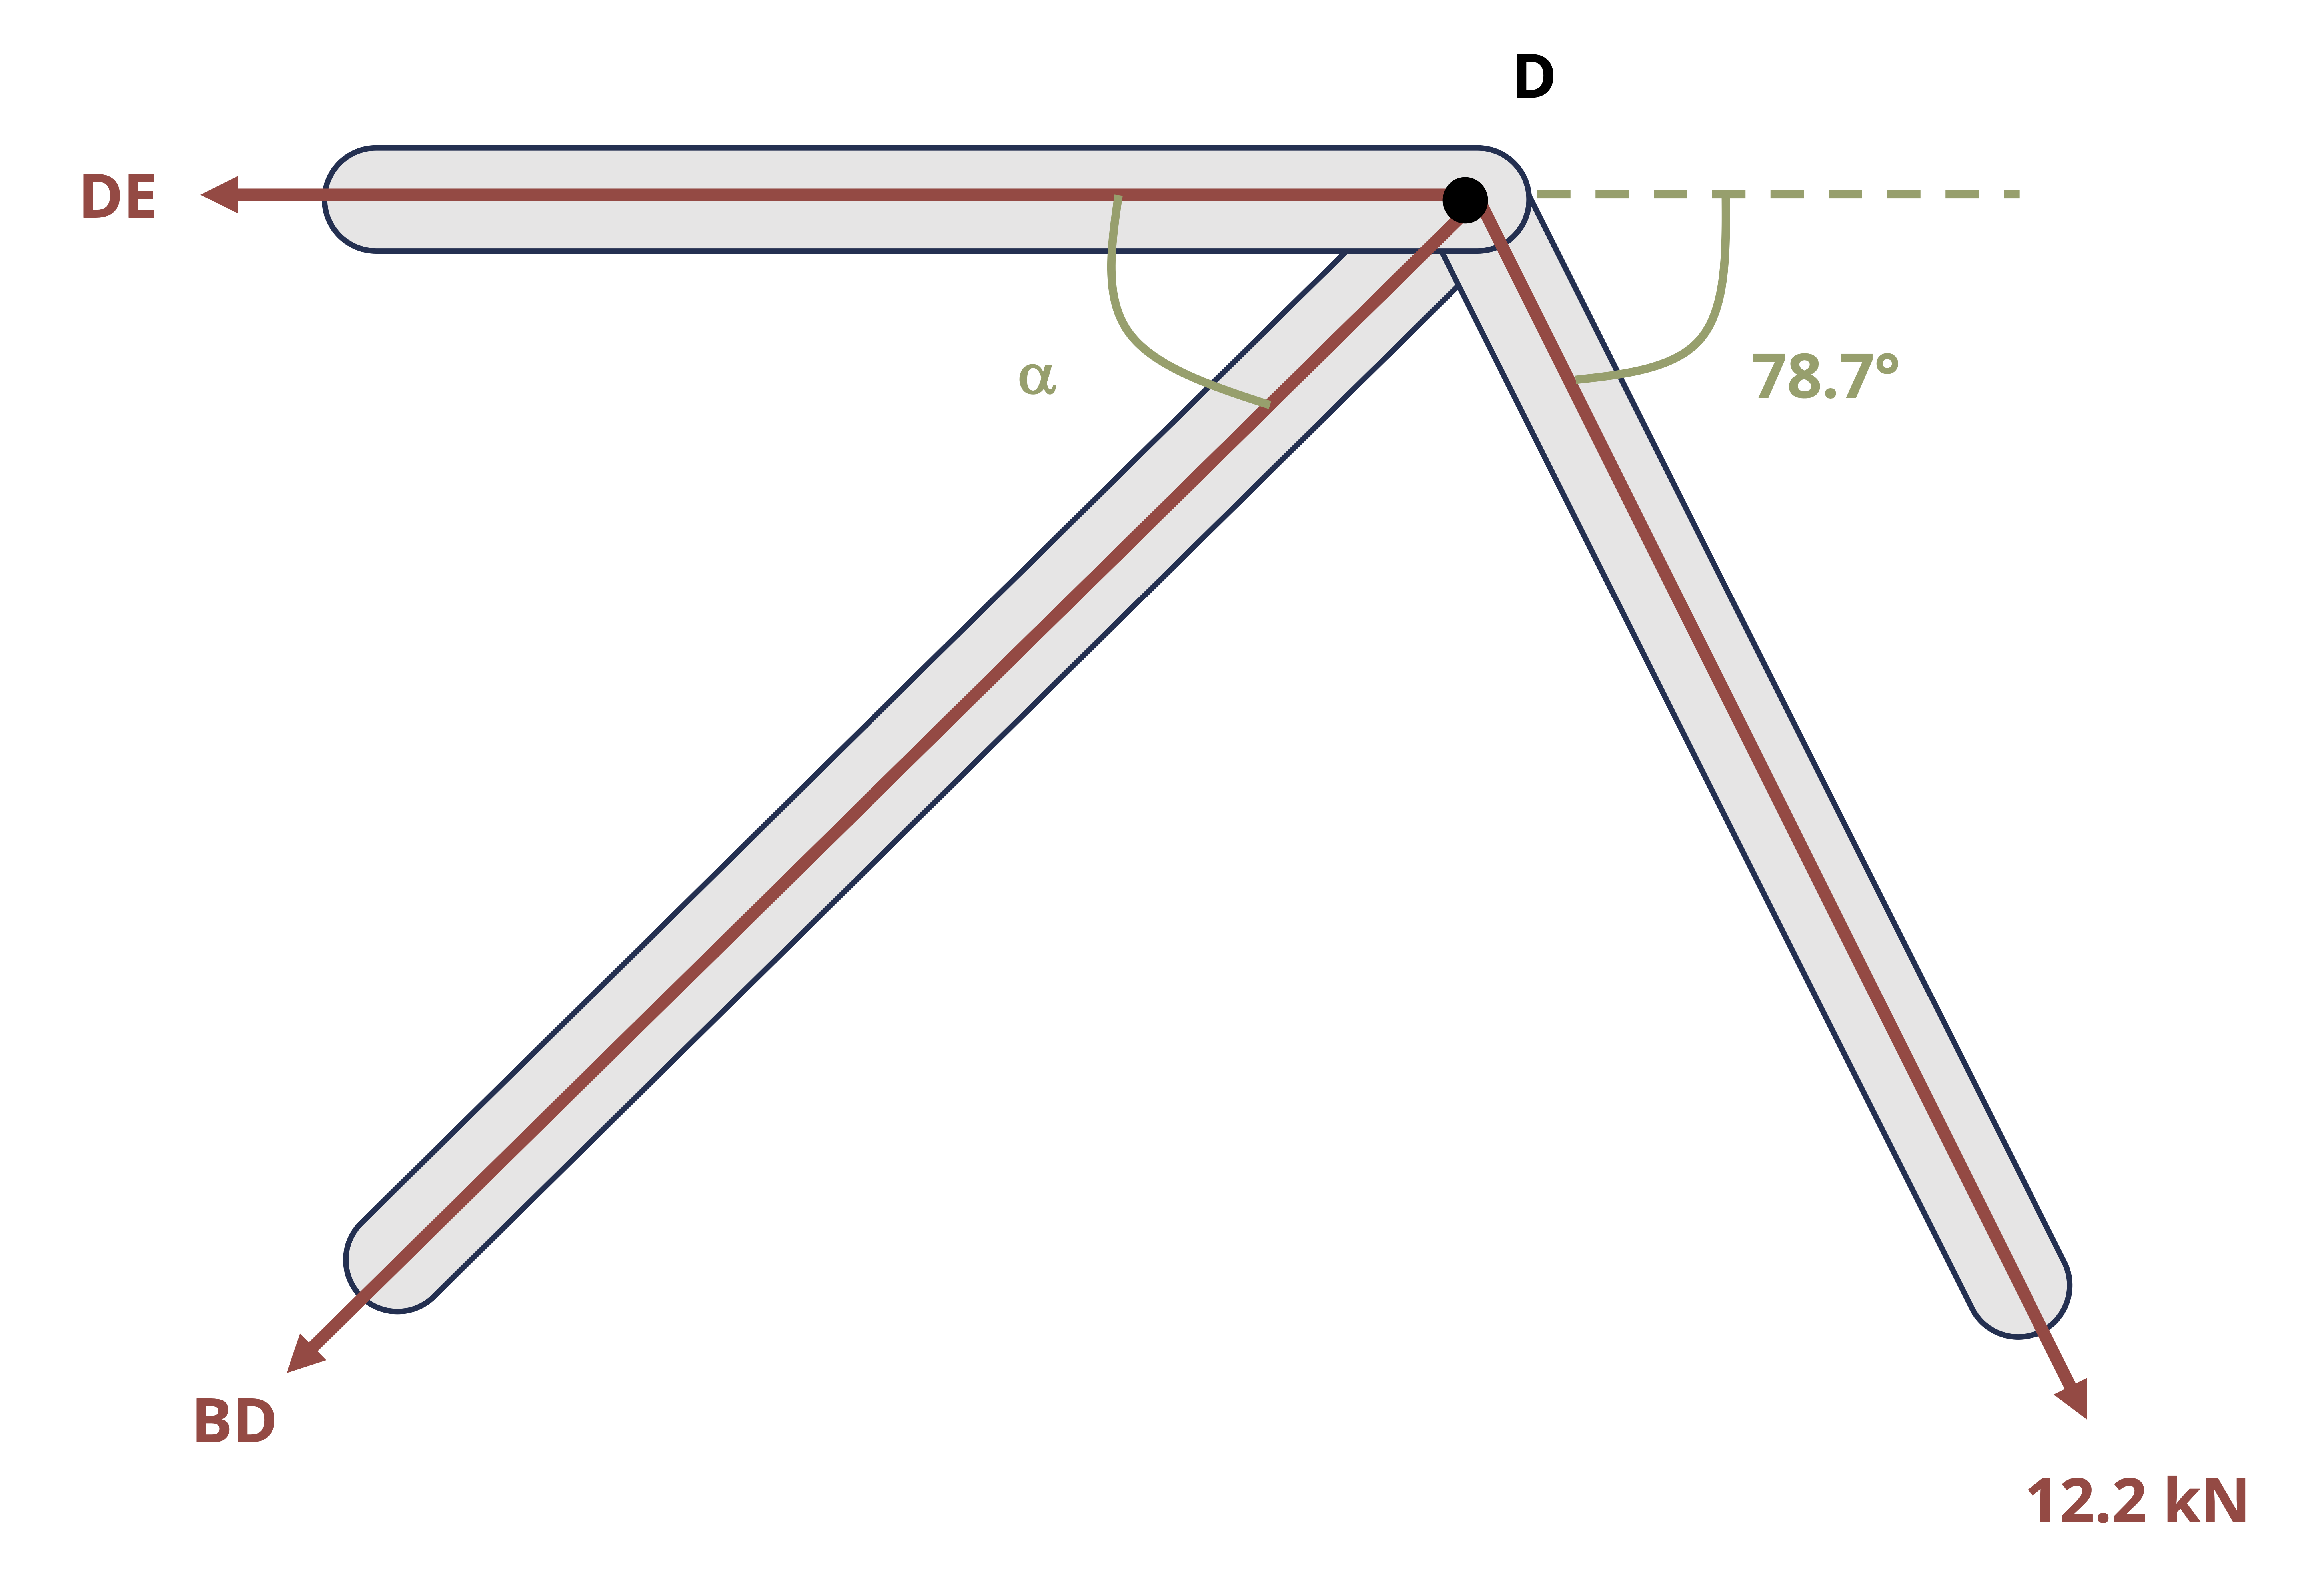
\includegraphics[width=3.625in,height=\textheight]{images/Updated CH1 examples/example 1.4 part 3.png}
\end{center}

We know the 12.2 kN force is at angle Θ=78.7° from horizontal. Angle α
can be found by considering right angle triangle BDE which has a base of
4 m and a height of 5 m. Once this angle is known, we can use
equilibrium equations to find the forces in members BD and DE.

\[
\alpha=\tan ^{-1}\left(\frac{5}{4}\right)=51.3^{\circ} \\
\\
\begin{aligned}
\sum F_y&=-12.2 \sin \left(78.7^{\circ}\right)-B D \sin \left(51.3^{\circ}\right)=0 \quad\rightarrow\quad B D=-15.3{~kN} \\
\sum F_x&=-D E-B D \cos \left(51.3^{\circ}\right)+12.2 \cos \left(78.7^{\circ}\right)=0 \\
&=-D E-(-15.3) \cos \left(51.3^{\circ}\right)+12.2 \cos \left(78.7^{\circ}\right)=0 \quad\rightarrow\quad D E=12{~kN}
\end{aligned}
\]

Force BD is 15.3 kN in compression and force DE is 12 kN in tension. Now
we need to find force BE. There are two remaining unknowns at joint B:
AB and BE.

FBD Joint B

\begin{center}
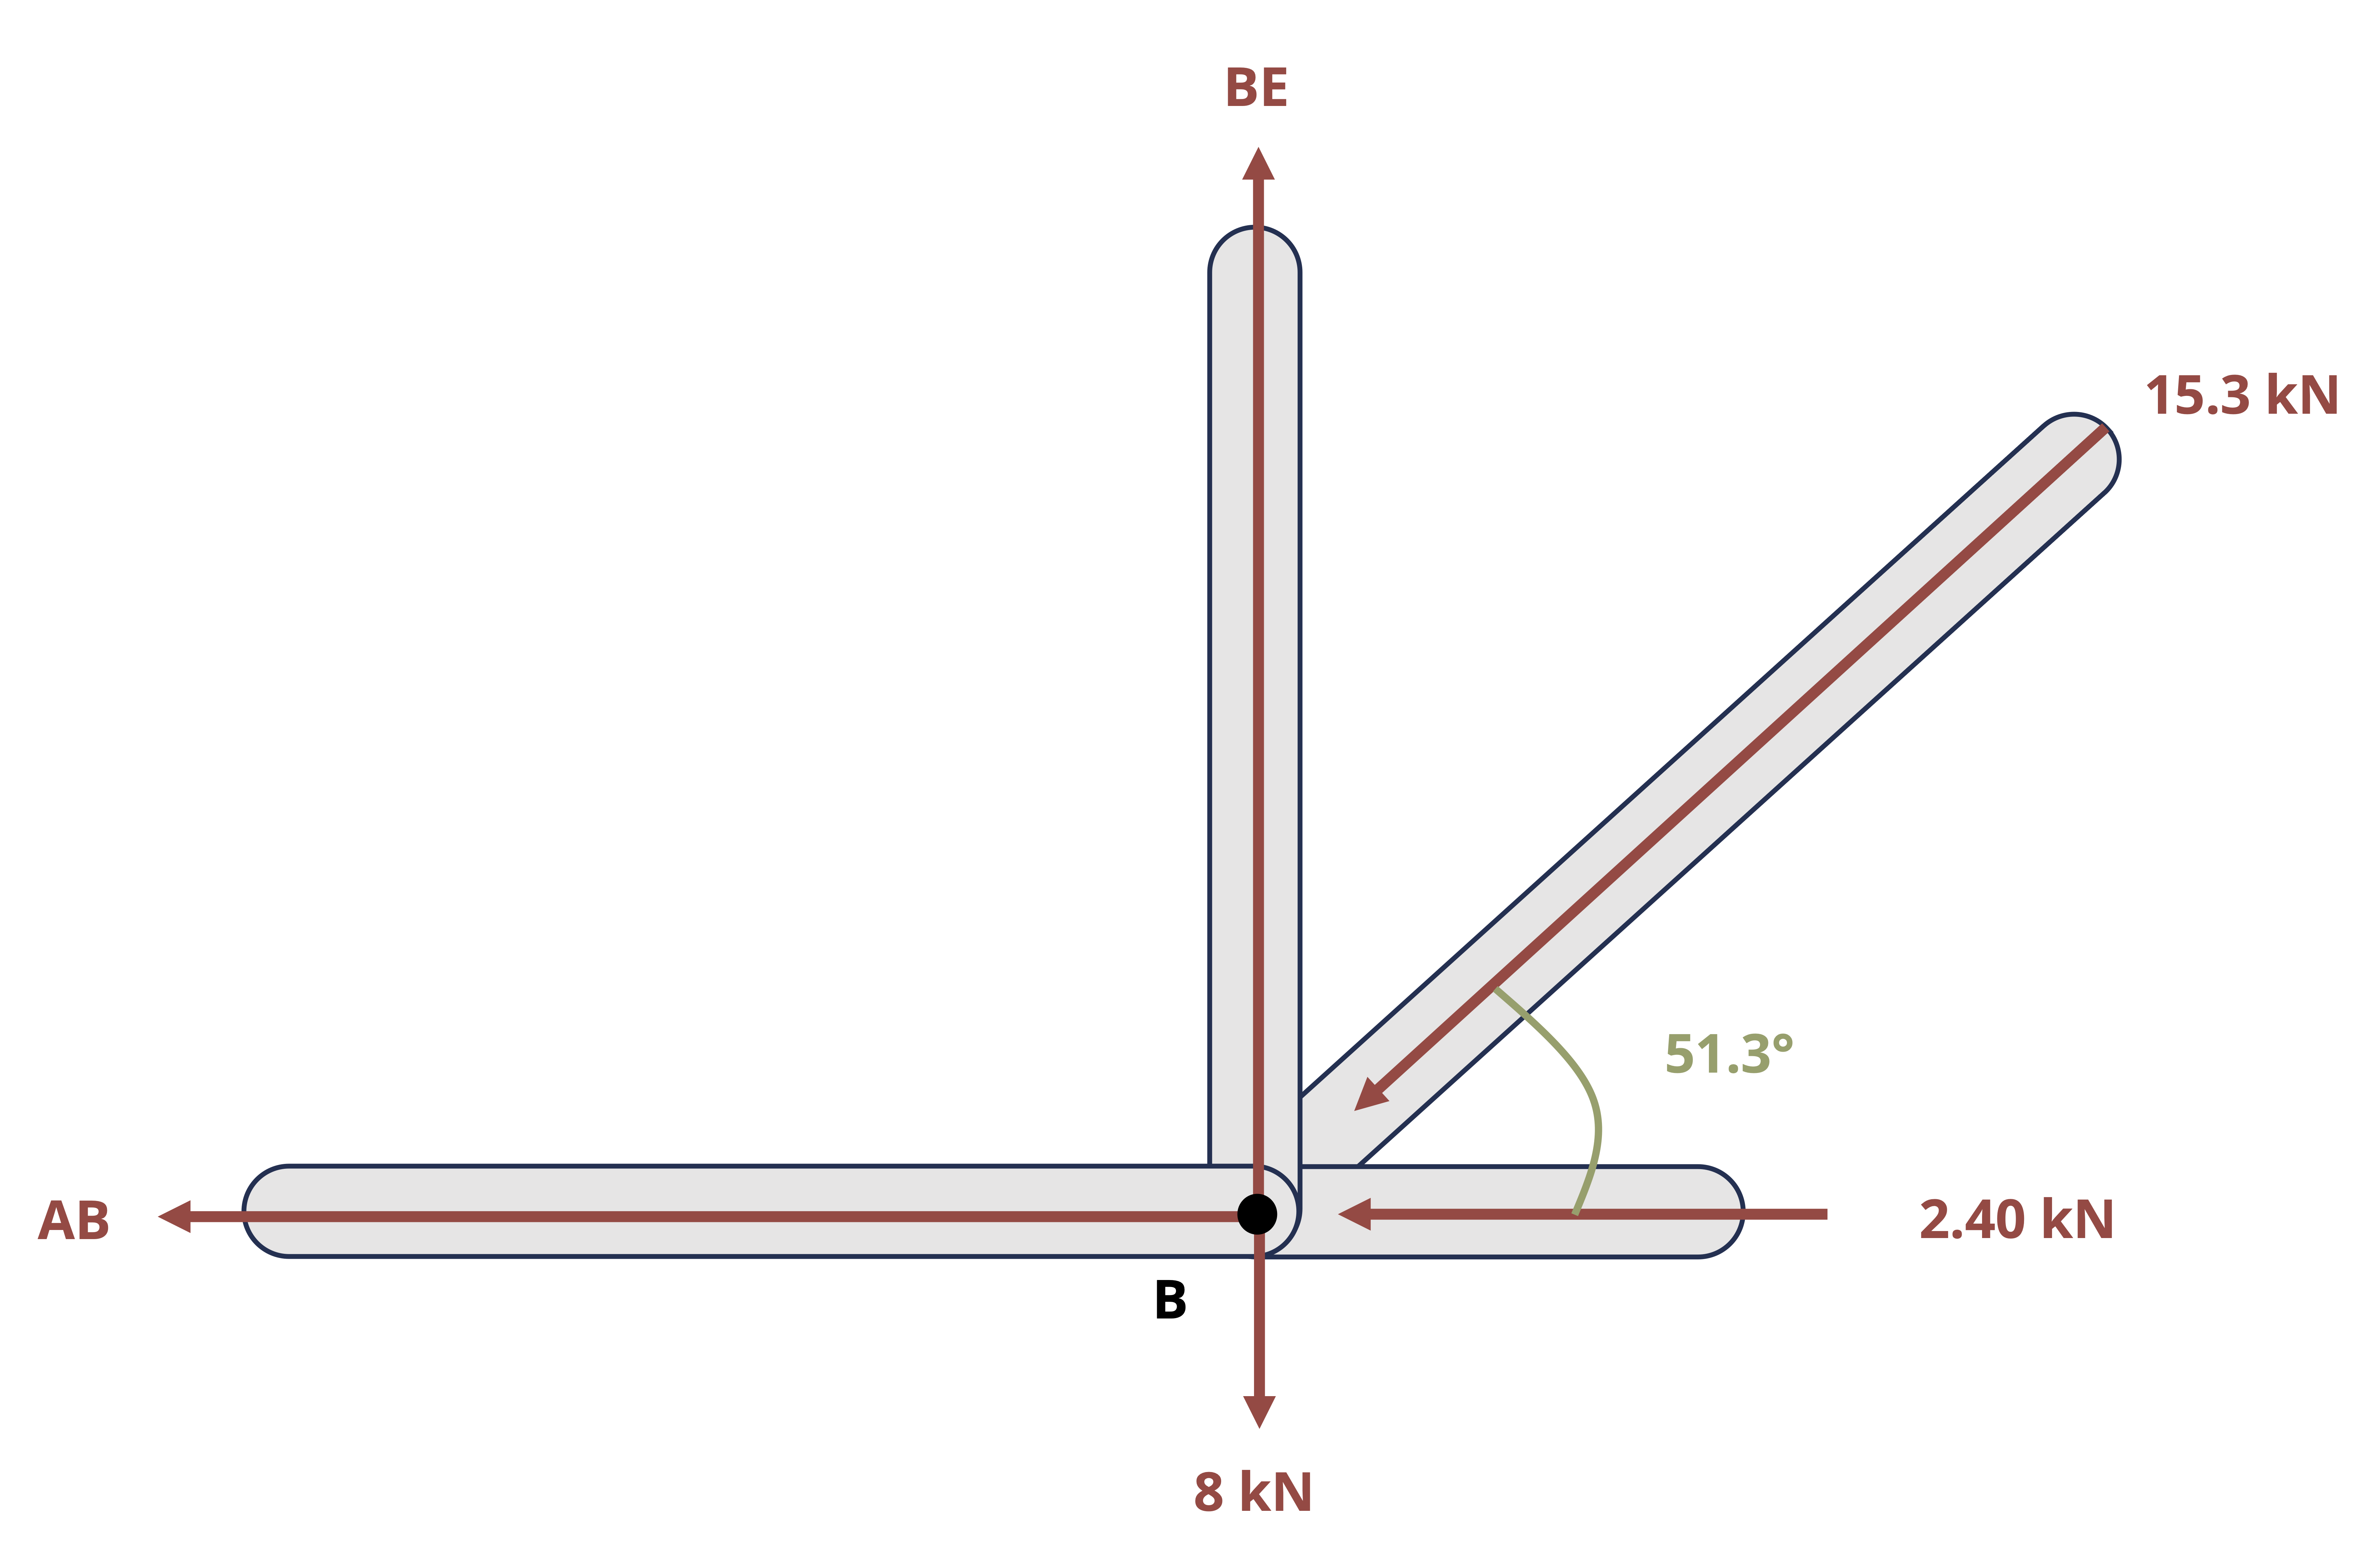
\includegraphics[width=4.5in,height=\textheight]{images/Updated CH1 examples/example 1.4 part 4.png}
\end{center}

\[
\sum F_y=B E-8-15.3 \sin \left(51.3^{\circ}\right)=0 \quad\rightarrow\quad B E=20{~kN}
\]

\textbf{Answer: DE = 12 kN (Tensile), BE = 20 kN (Tensile)}

\end{tcolorbox}

\begin{tcolorbox}[enhanced jigsaw, colback=white, colframe=quarto-callout-tip-color-frame, toptitle=1mm, arc=.35mm, bottomrule=.15mm, toprule=.15mm, opacitybacktitle=0.6, title={Solution - Method of Sections}, coltitle=black, breakable, colbacktitle=quarto-callout-tip-color!10!white, bottomtitle=1mm, titlerule=0mm, opacityback=0, leftrule=.75mm, left=2mm, rightrule=.15mm]

While Method of Joints can be used here, it is inefficient. We needed to
draw and analyze free body diagrams of joints C, D, and B and keep track
of the forces at these joints as well as whether each force was in
tension or compression.

Method of Sections may be used as an alternative to find forces BE and
DE. To apply Method of Sections, we should cut through no more than 3
unknown members and draw a free body diagram with no more than 3 total
unknowns. For this problem, make a cut through the truss that passes
through members AB, BE, and DE.

\begin{center}
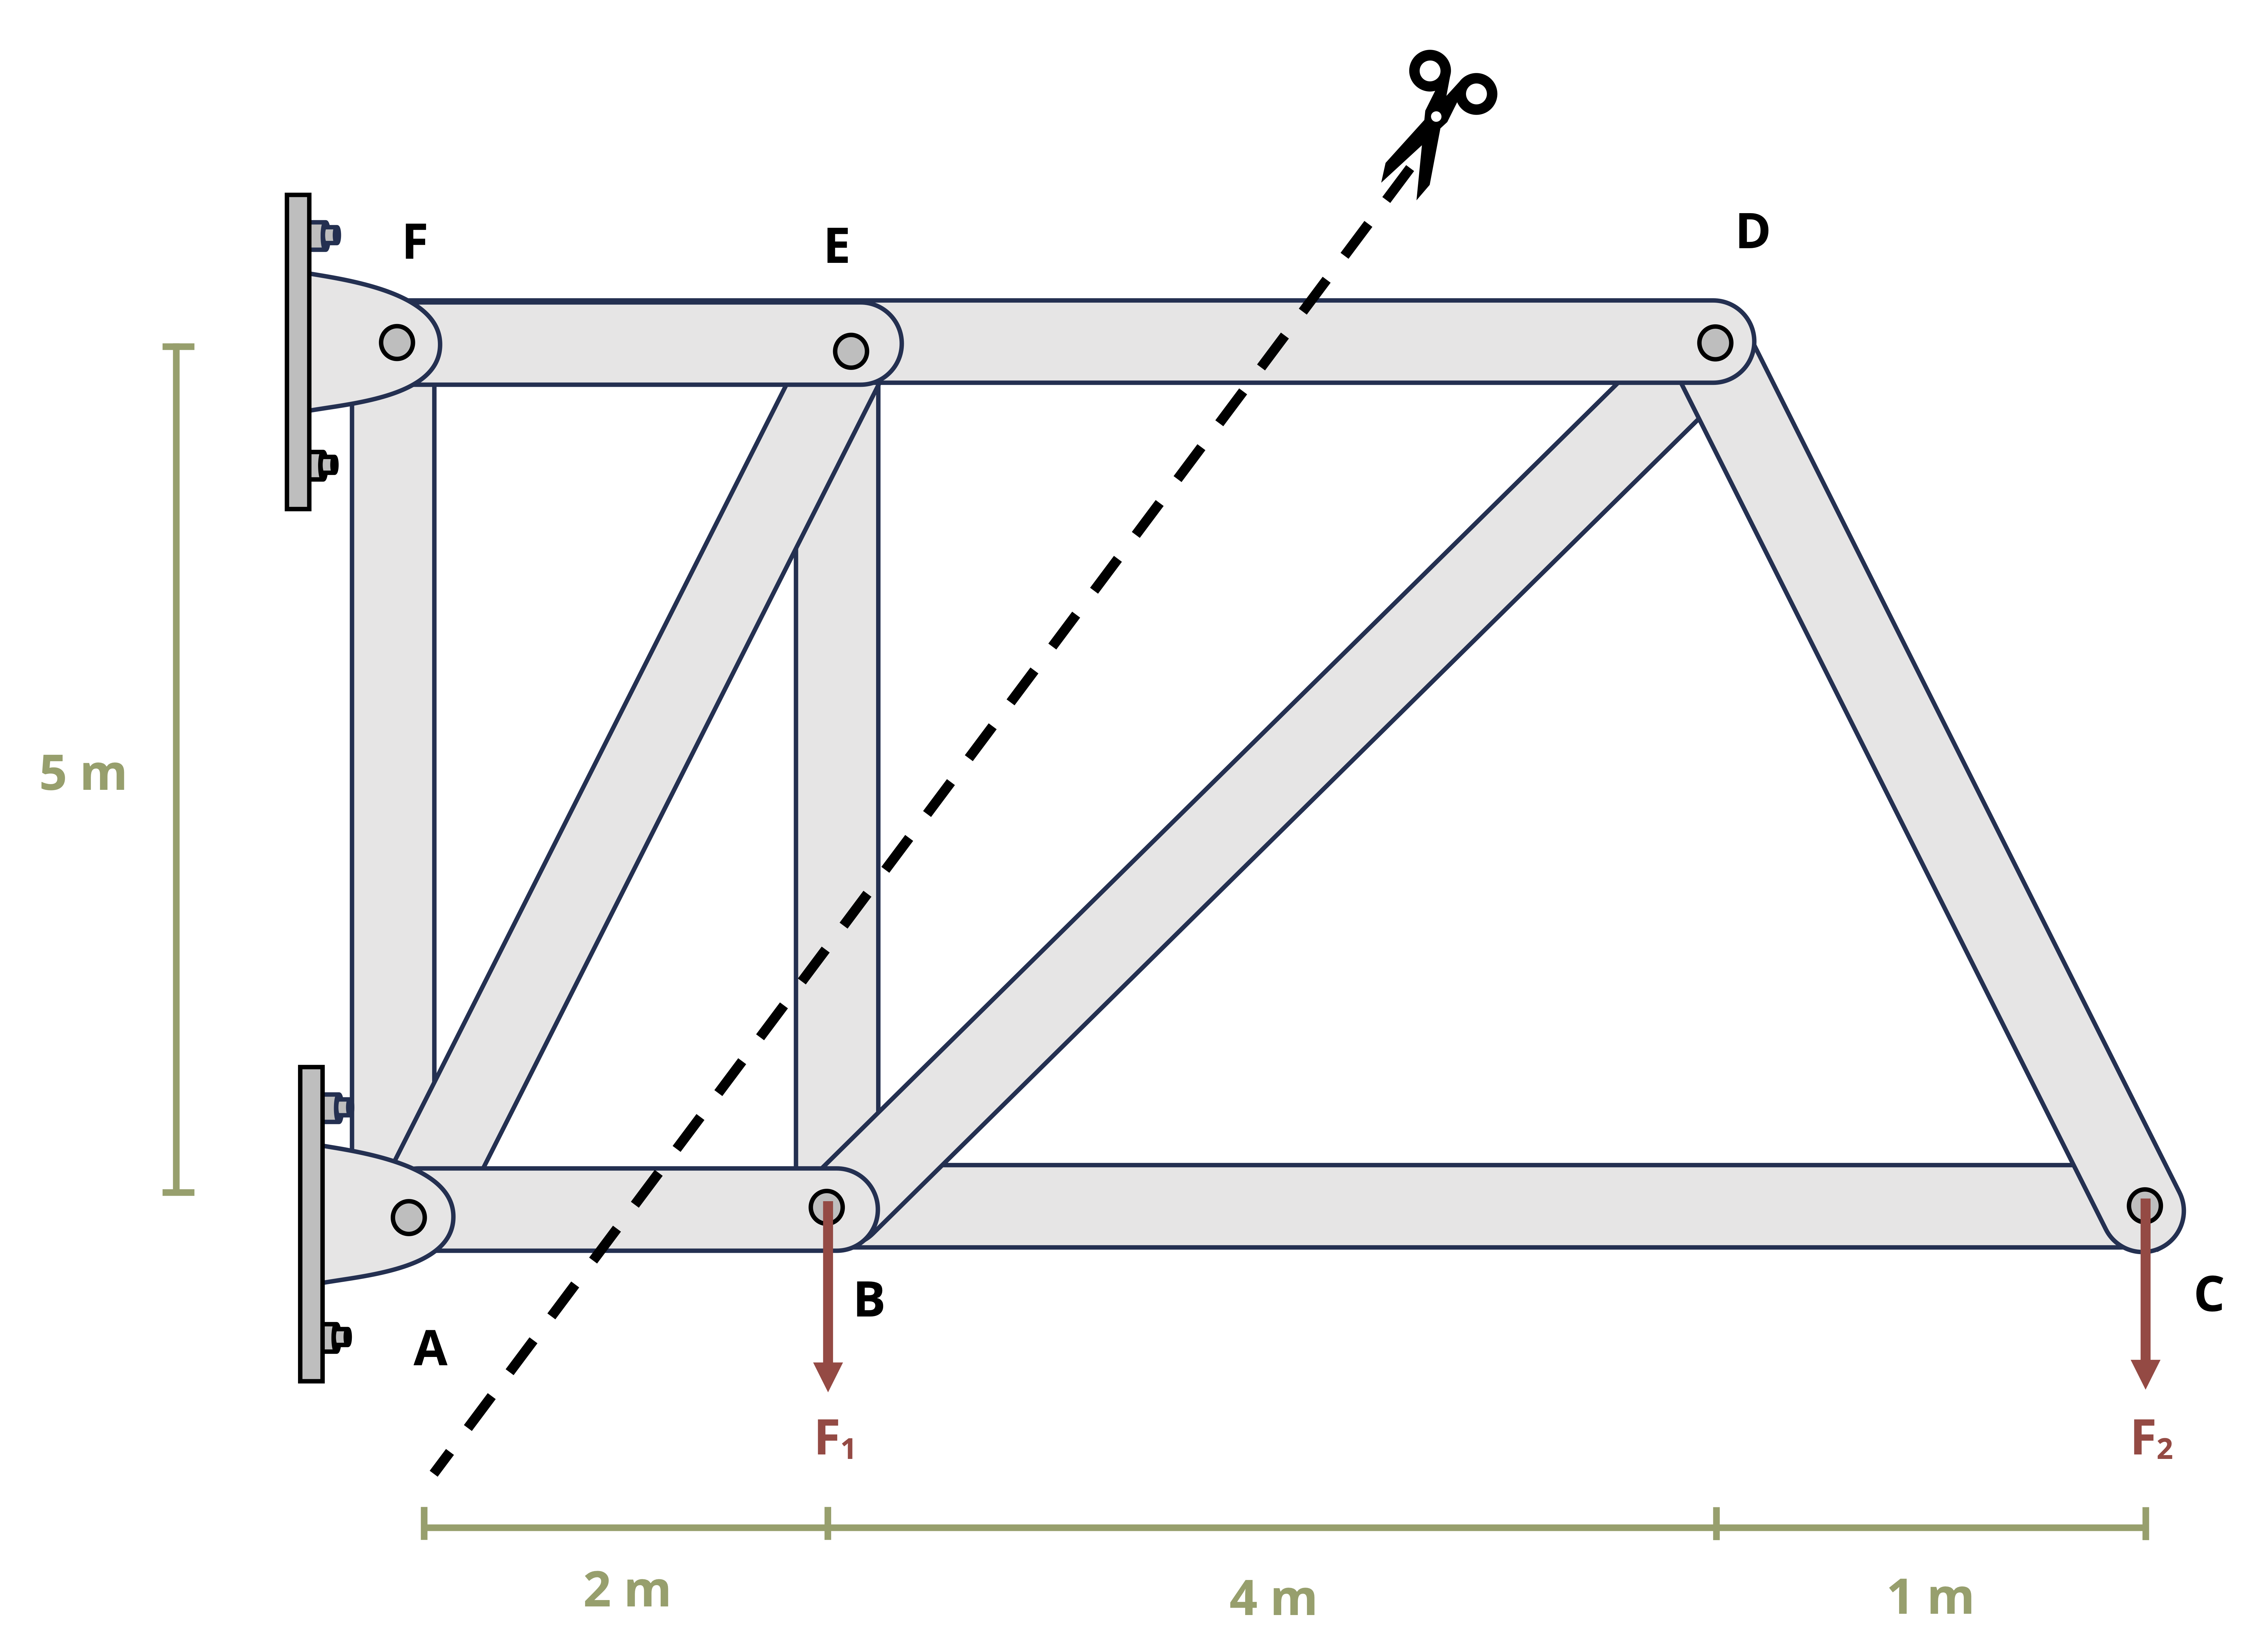
\includegraphics[width=4.55208in,height=\textheight]{images/Updated CH1 examples/example 1.4 part 5.png}
\end{center}

Once that cut is made, a choice needs to be made to draw an FBD for the
intact part of the truss to the left of the cut or the intact part of
the truss to the right of the cut~ Either way, the external forces on
the side would need to be shown on the FBD as well as the force of each
member that was cut through.

If we chose the left side, there would be unknowns AB, BE, and DE, as
well as unknown reactions Ax, Fx, and Fy. However, on the right side
there are no unknown support reactions so the only unknowns are forces
AB, BE, and DE.

\begin{center}
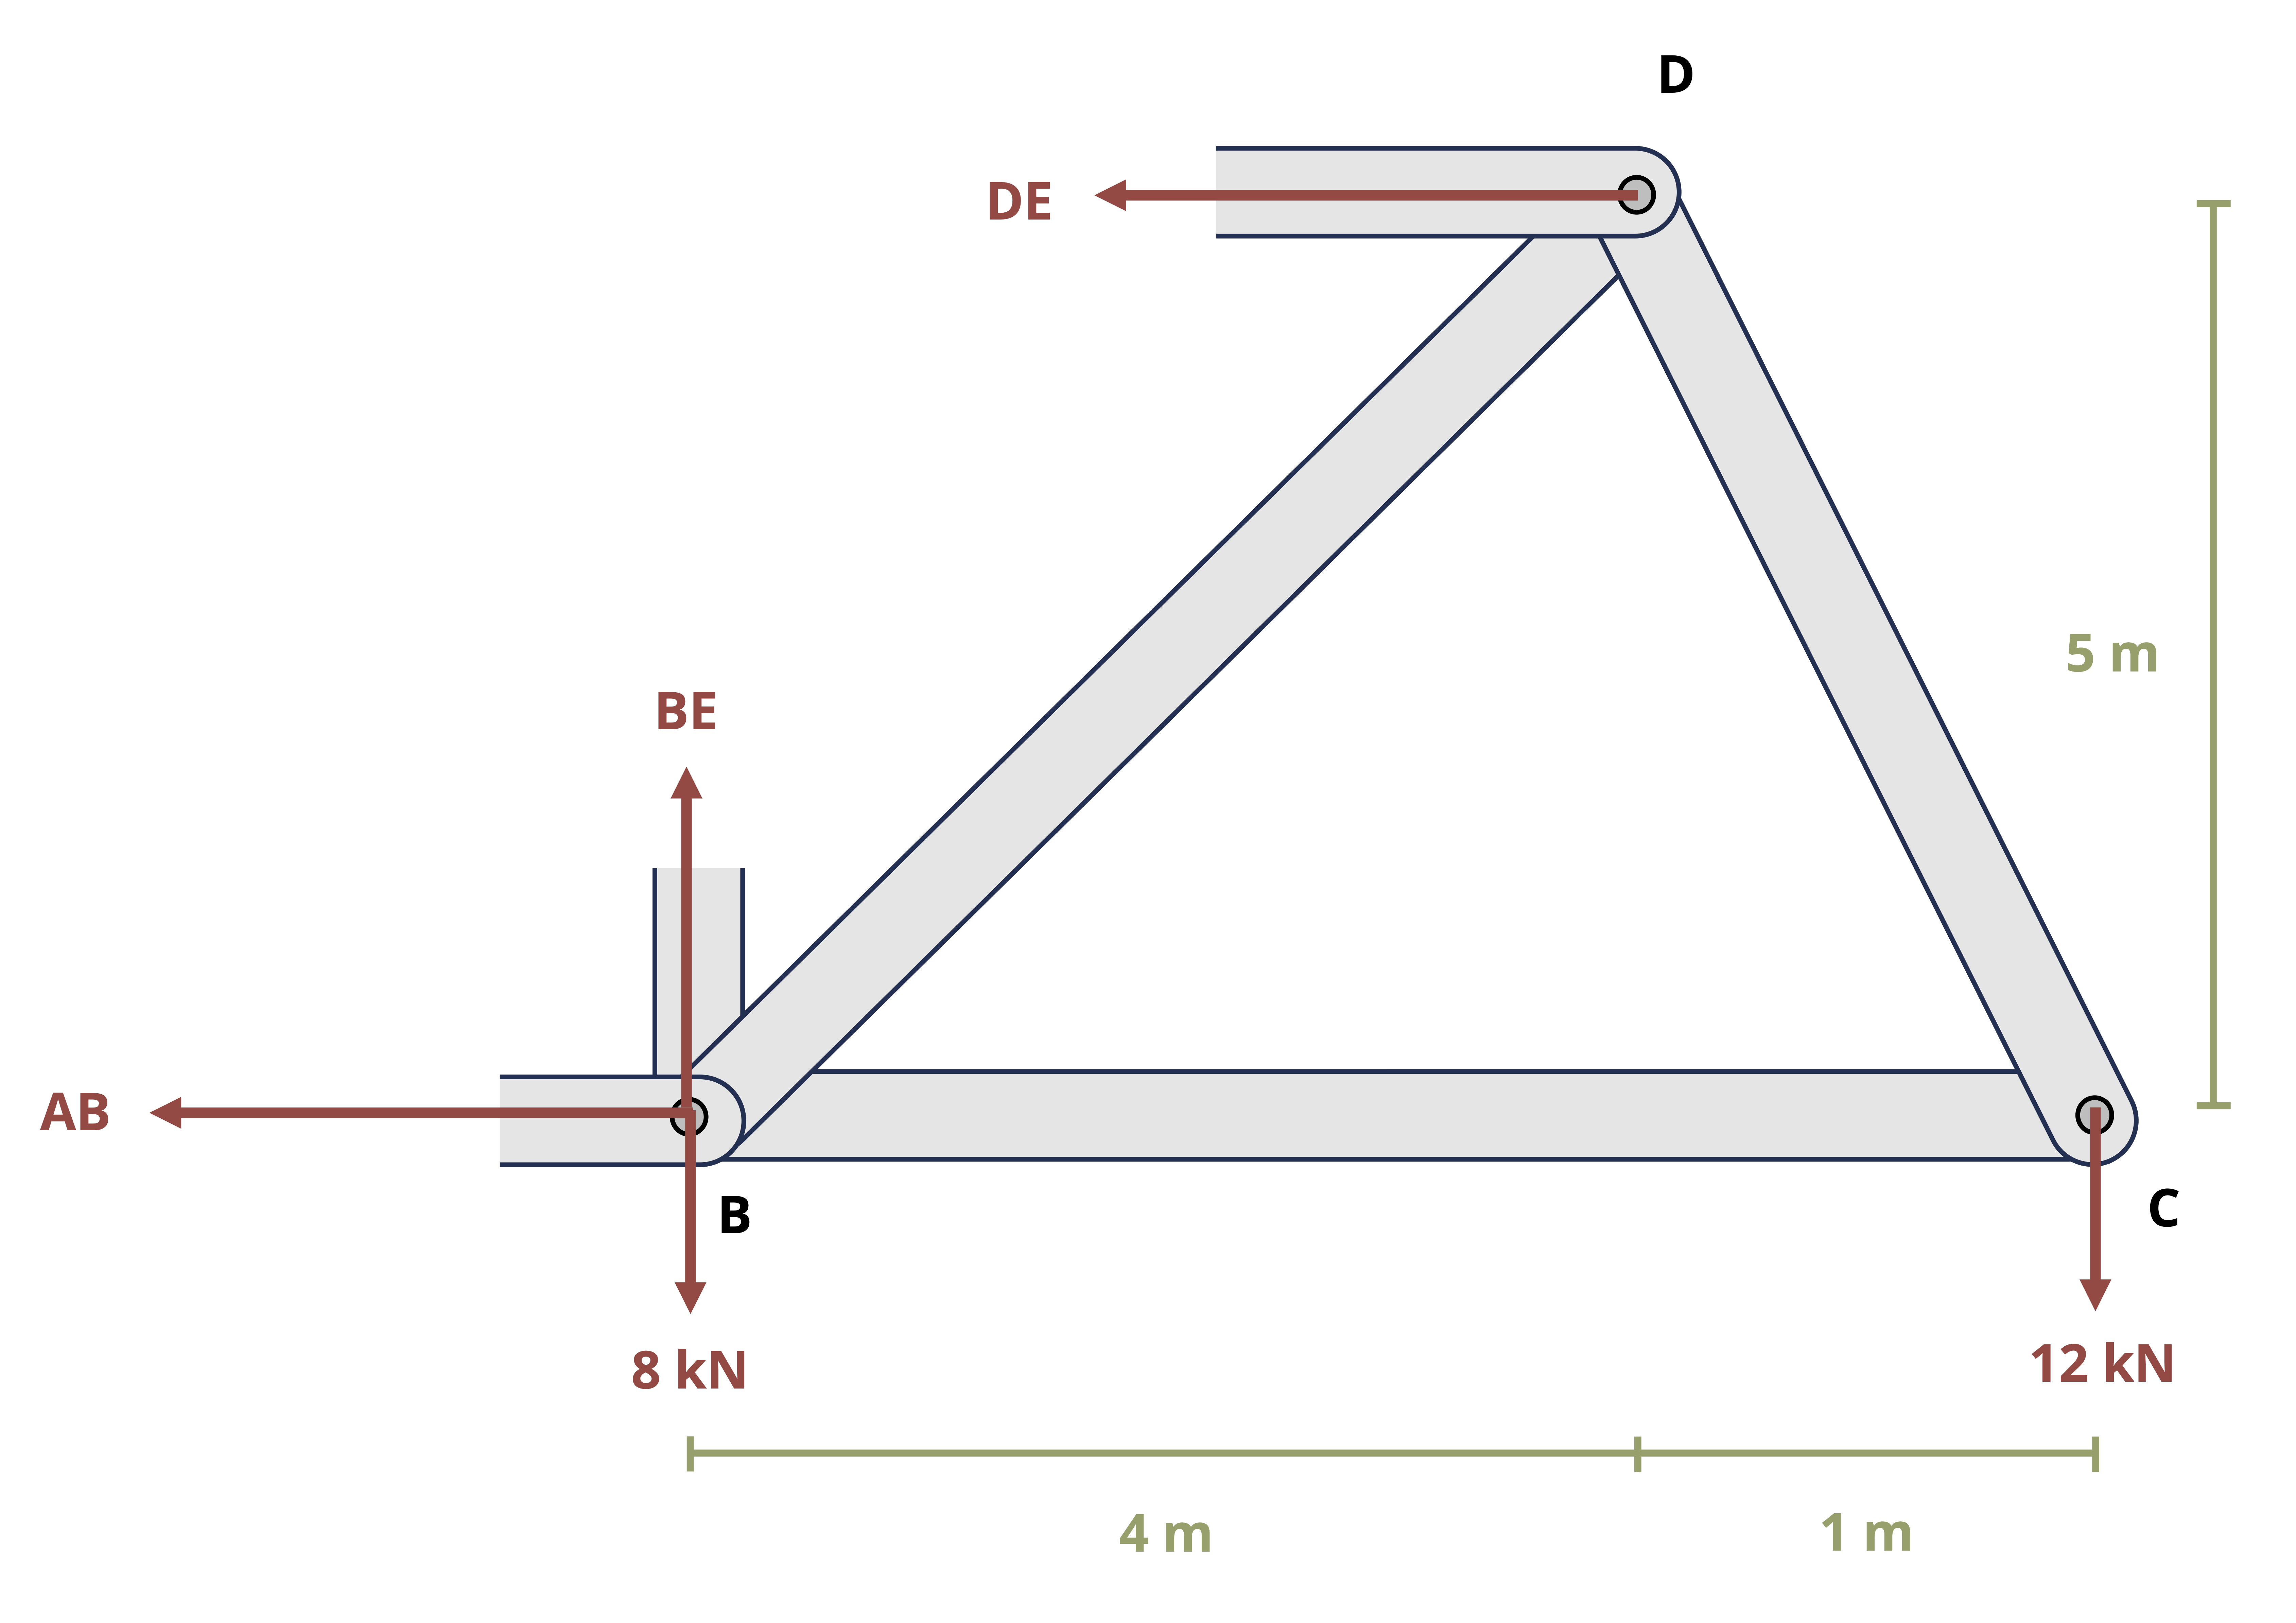
\includegraphics[width=4.6875in,height=\textheight]{images/Updated CH1 examples/example 1.4 part 6.png}
\end{center}

\[
\begin{aligned}
& \sum M_B=-(12*5)+(DE*5)=0 \quad\rightarrow\quad D E=12{~kN} \\
& \sum F_y=BE-8-12=0 \quad\rightarrow\quad B E=20{~kN}
\end{aligned}
\]

Once again, the forces are drawn on the FBD in the tensile direction, so
the positive answers indicate the forces are indeed tensile.

\textbf{Answer: DE = 12 kN (Tensile), BE = 20 kN (Tensile)}

\end{tcolorbox}

\end{example}

\end{tcolorbox}

\subsection{Internal reactions in continuous
bodies}\label{internal-reactions-in-continuous-bodies}

Internal reactions also exist within a body or structure. These
reactions are necessary to hold the body together and will vary from
point to point in a body depending on the distribution of external
loading. As shown in Figure~\ref{fig-1.2}, the reactions at any given
point can be examined by making a cut at the point of interest in the
body. One can think of any point within a body as acting as a fixed
support for the rest of the body. That is, every point must potentially
exert a force parallel to the cross section where the cut is made which
is the shear force V, a force perpendicular to the cross section where
the cut is made which is the normal force N, and a reaction moment where
the cut is made which is the bending moment M. Moreover, as was
discussed for internal pin reactions and the cut made for Method of
Sections for trusses, the reactions at a cut will be equal and opposite
on the two sides of the cut.

\begin{figure}

\centering{

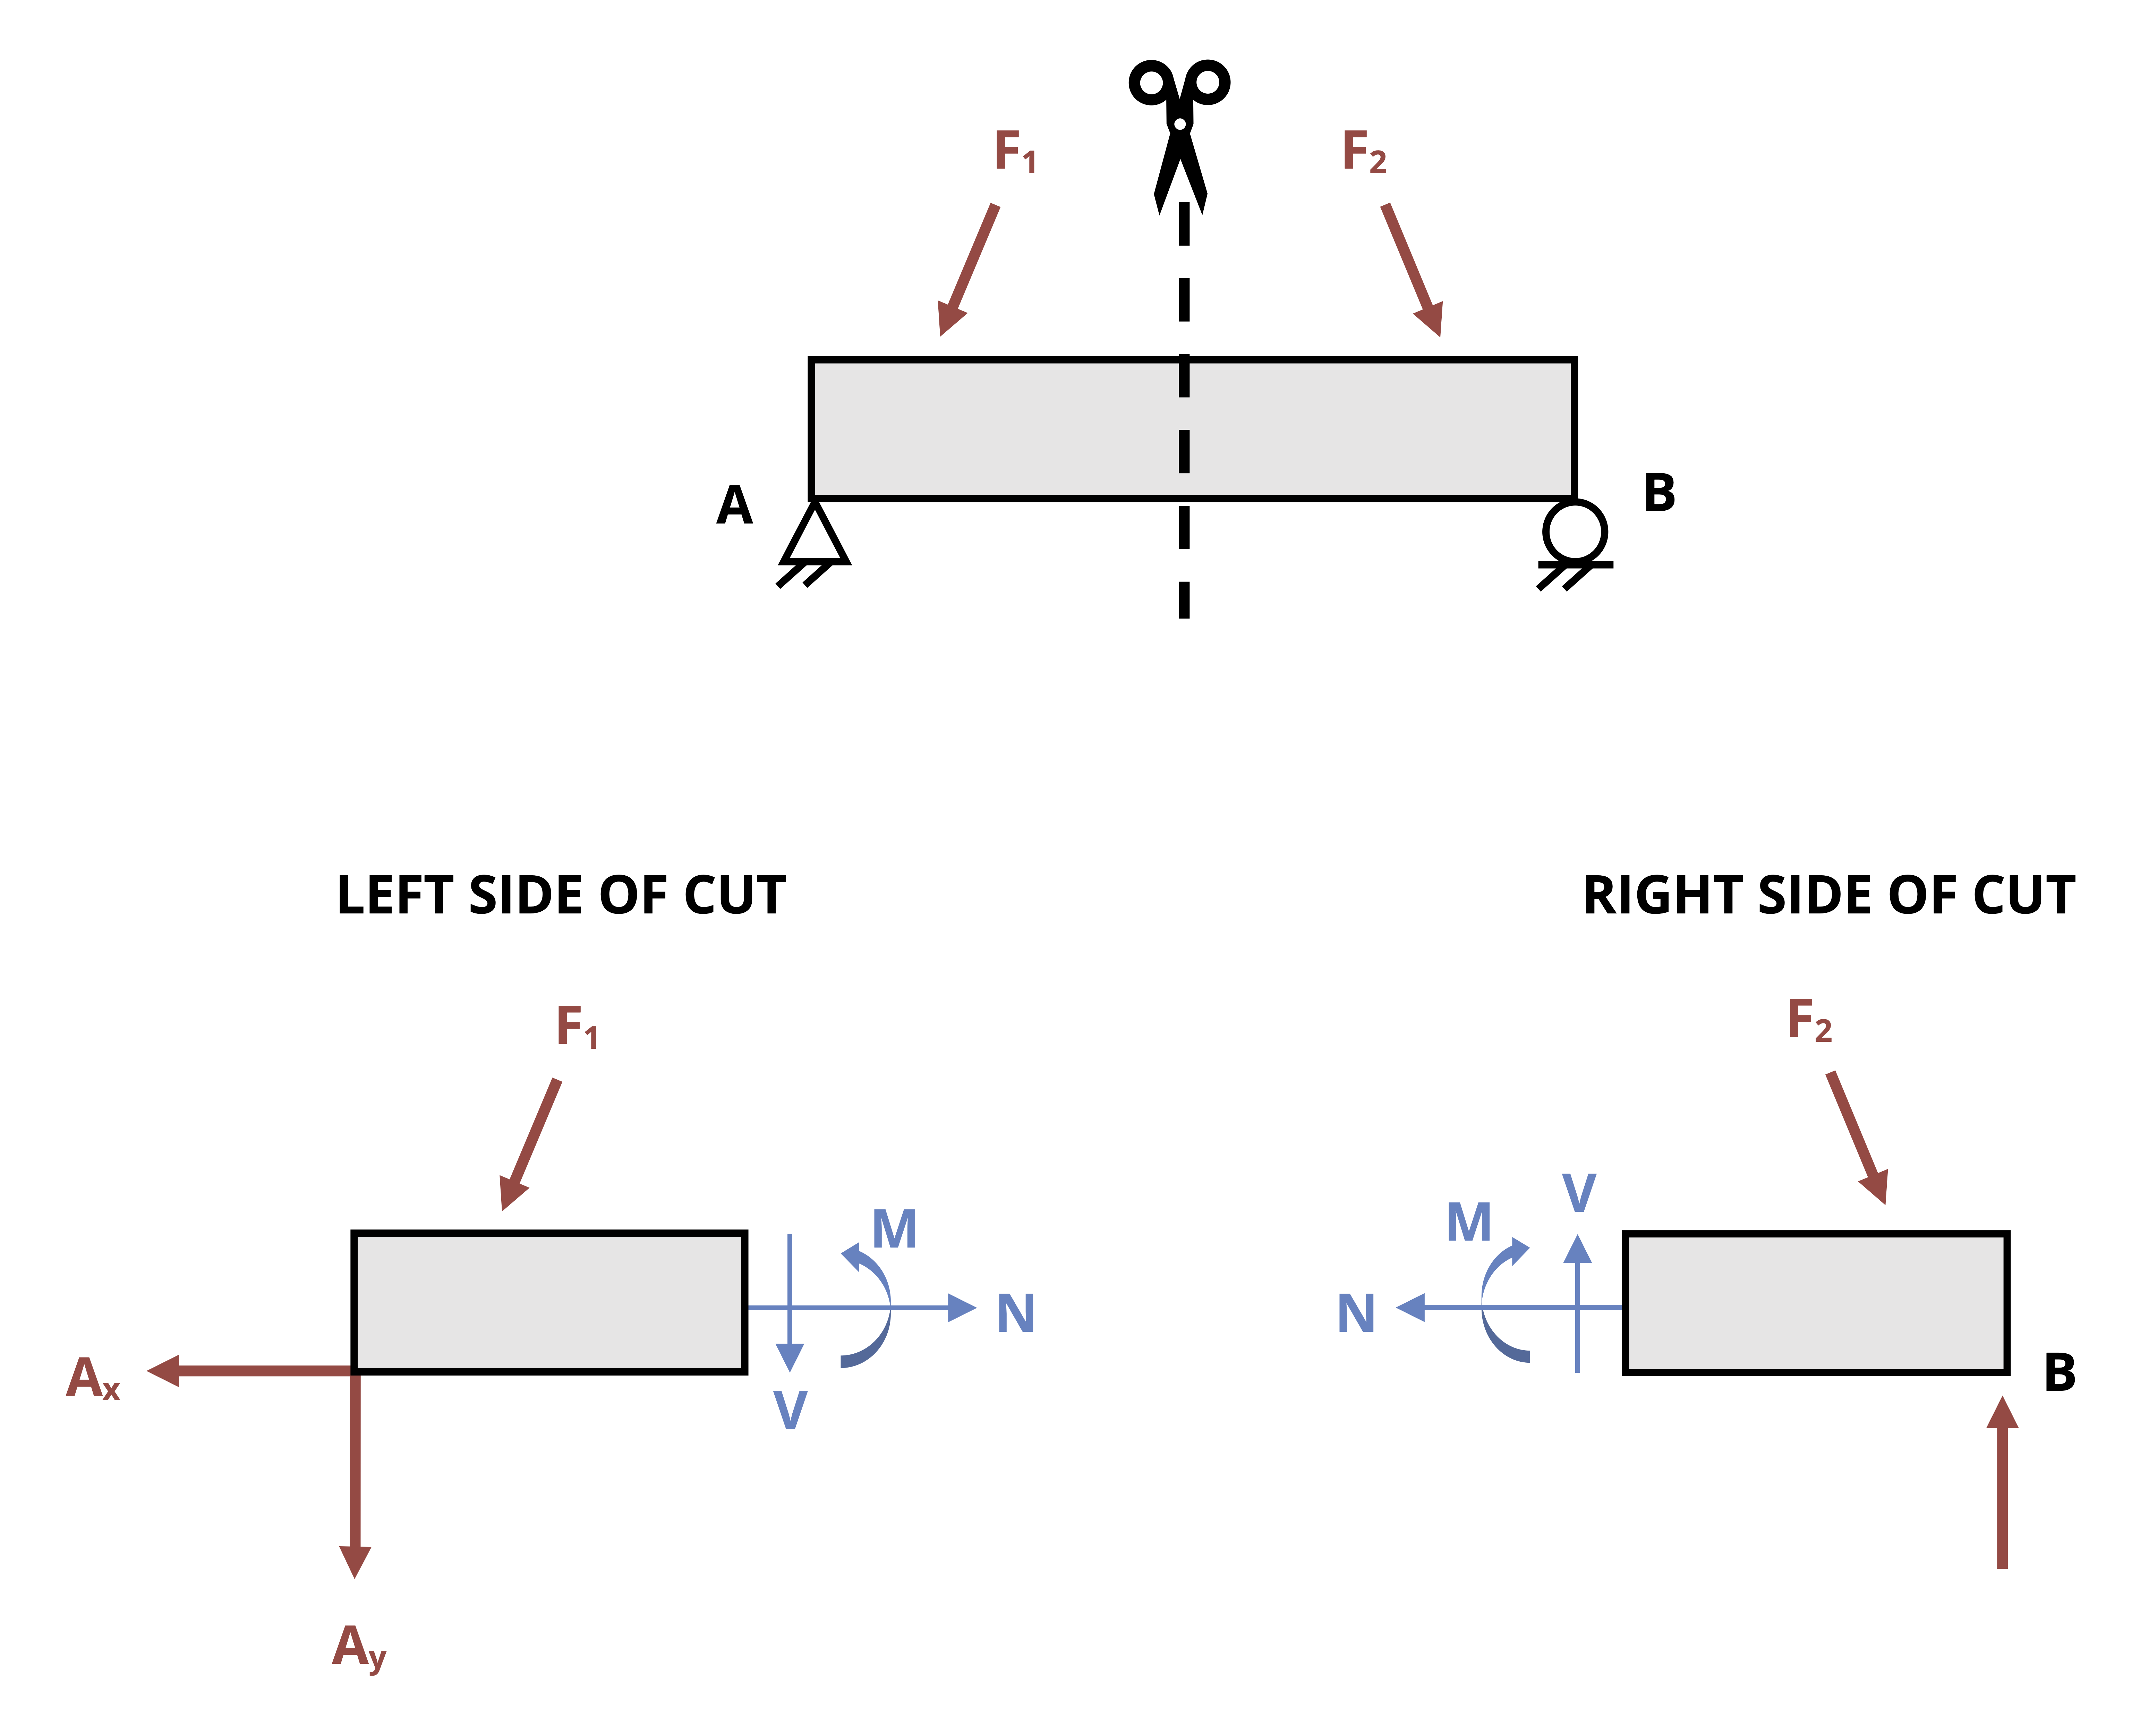
\includegraphics[width=5.03125in,height=\textheight]{images/CH1 PNGs/figure 1.2.png}

}

\caption{\label{fig-1.2}Cross-sections showing the internal loads on a
continuous body}

\end{figure}%

To determine the reactions, the FBD of the part of the beam to the left
of the cut can be drawn and used, or the part of the beam to the right
of the cut can be drawn and used. As was discussed with Method of
Sections for trusses, the choice of which side of the cut to examine is
based primarily on which side appears easiest and most efficient to
analyze. Once the FBD of the cut section is drawn, the three equilibrium
equations can be applied to determine the internal reactions. The
determination of shear and bending moments in beams will be reviewed in
more detail in Chapter~\ref{sec-beams}. The focus of
Example~\ref{exm-1.5} is on the determination of the normal force, as
this will be important in Chapter~\ref{sec-stress} and
Chapter~\ref{sec-strain}.

\begin{tcolorbox}[enhanced jigsaw, colback=white, colframe=quarto-callout-tip-color-frame, toptitle=1mm, arc=.35mm, bottomrule=.15mm, toprule=.15mm, opacitybacktitle=0.6, title={Example 1.5}, coltitle=black, breakable, colbacktitle=quarto-callout-tip-color!10!white, bottomtitle=1mm, titlerule=0mm, opacityback=0, leftrule=.75mm, left=2mm, rightrule=.15mm]

\begin{example}[]\protect\hypertarget{exm-1.5}{}\label{exm-1.5}

~

Two solid bars make up the axial assembly loaded as shown. Determine the
normal force in each bar. State whether the force is tensile or
compressive.

\begin{center}
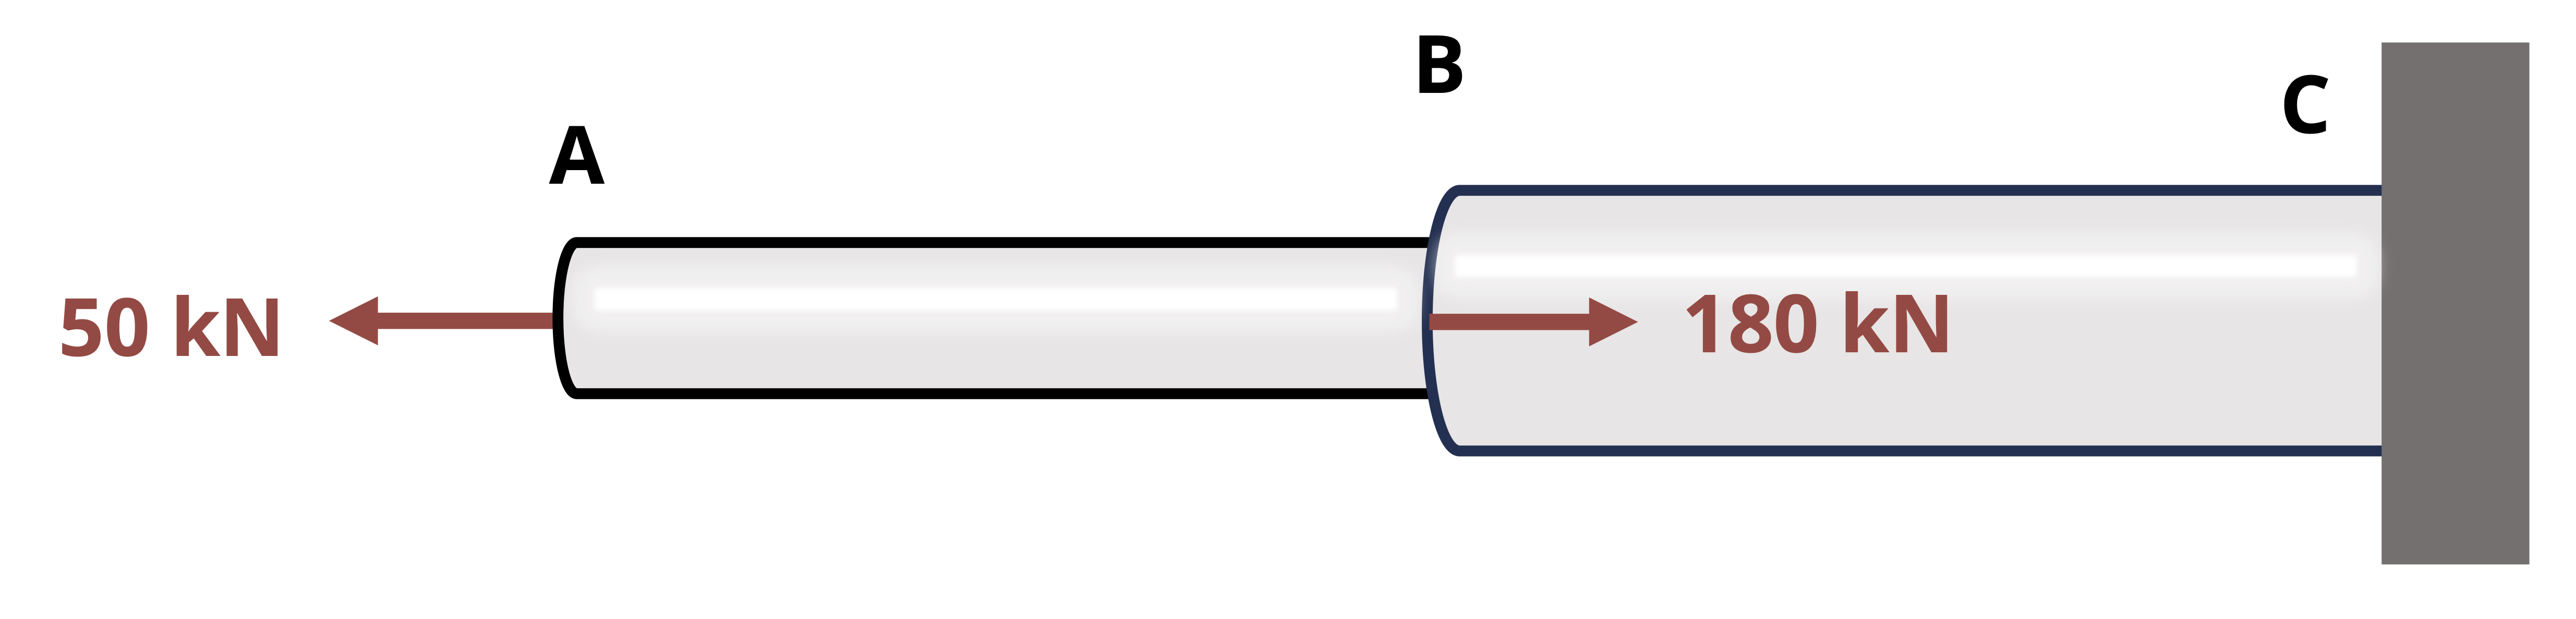
\includegraphics[width=4.46875in,height=\textheight]{images/Updated CH1 examples/example 1.5 part 1.png}
\end{center}

\begin{tcolorbox}[enhanced jigsaw, colback=white, colframe=quarto-callout-tip-color-frame, toptitle=1mm, arc=.35mm, bottomrule=.15mm, toprule=.15mm, opacitybacktitle=0.6, title={Solution}, coltitle=black, breakable, colbacktitle=quarto-callout-tip-color!10!white, bottomtitle=1mm, titlerule=0mm, opacityback=0, leftrule=.75mm, left=2mm, rightrule=.15mm]

Though the assembly is not a beam, determining the internal reactions
will work in the same way. In this particular case, all the forces are
in the normal direction (no shear force) and due to the central
placement of the 60 kN force and the symmetry of the 125 kN forces,
there will be also be no bending moment. Consequently, only the normal
reaction force will be drawn on the FBDs.

To find the internal load in a segment, cut a cross-section within that
segment. Since the external loading (and therefore the internal loading)
changes at point B, we'll make one cut in segment AB and another in
segment BC.

Making the cut in section AB and drawing the FBD allows us to determine
the normal force in section AB. Note that drawing the left section of
the cut for the FBD results in avoiding needing to know the external
reactions at wall C.

\begin{center}
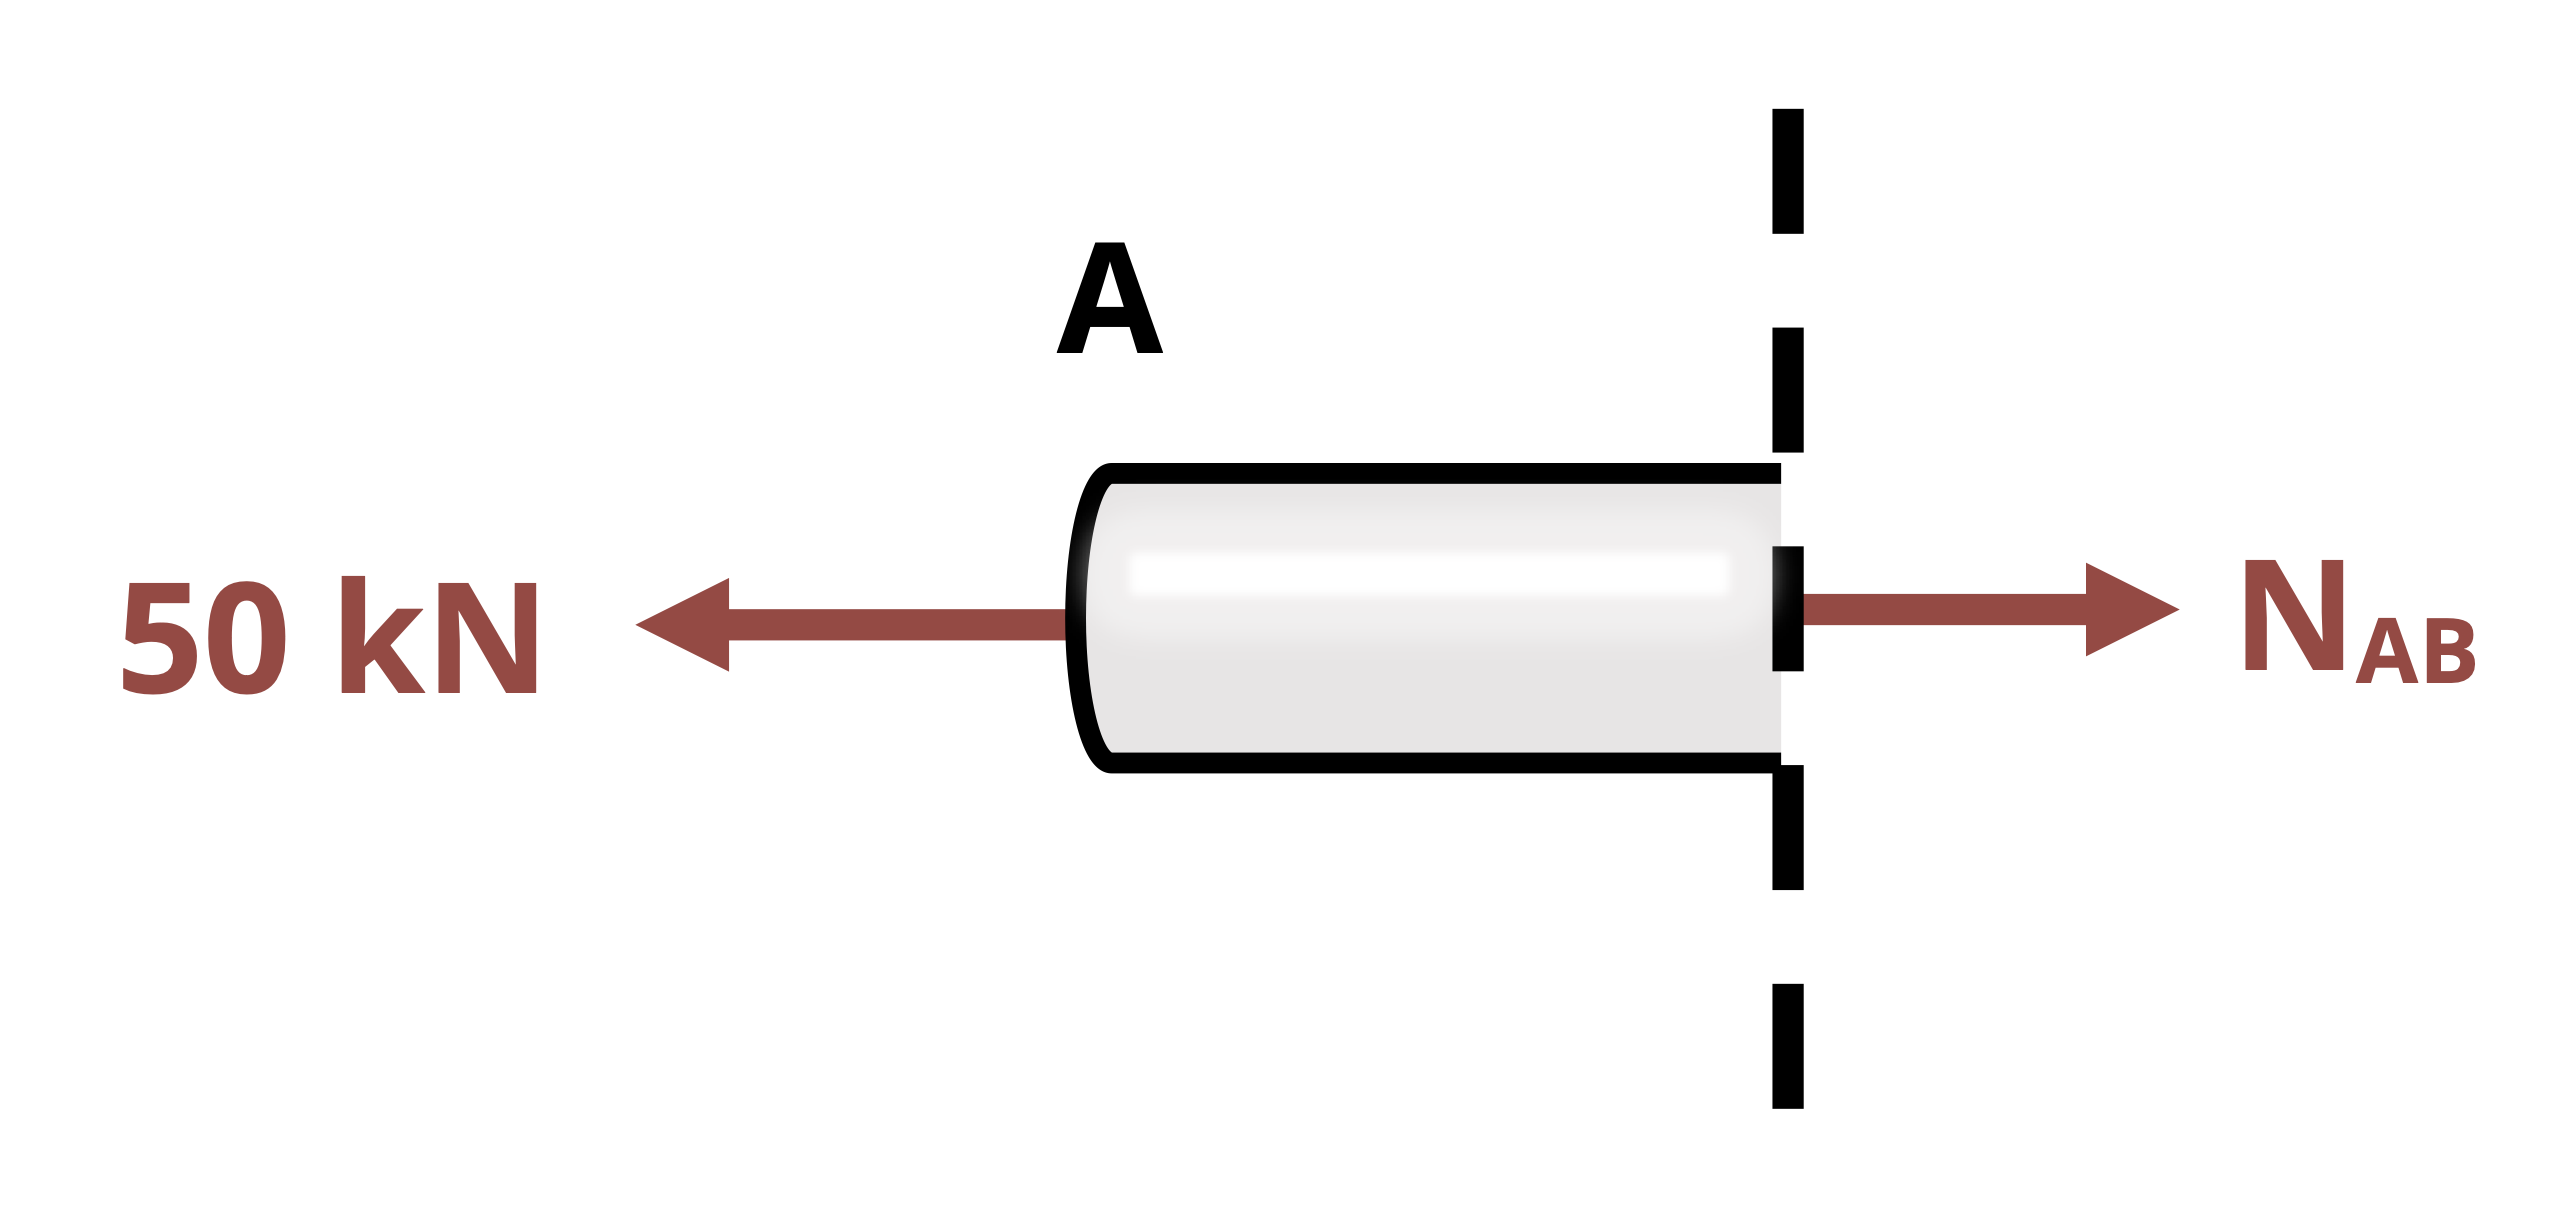
\includegraphics[width=2.07292in,height=\textheight]{images/Updated CH1 examples/example 1.5 part 2.png}
\end{center}

\[
\sum F_x=-50{~kN}+N_{AB}=0 \quad\rightarrow\quad N_{AB}=50{~kN}
\]

Making the cut in section BC and drawing the FBD allows us to determine
the normal force in section BC. Once again, drawing the left section of
the cut for the FBD results in avoiding needing to know the external
reactions at wall C.

\begin{center}
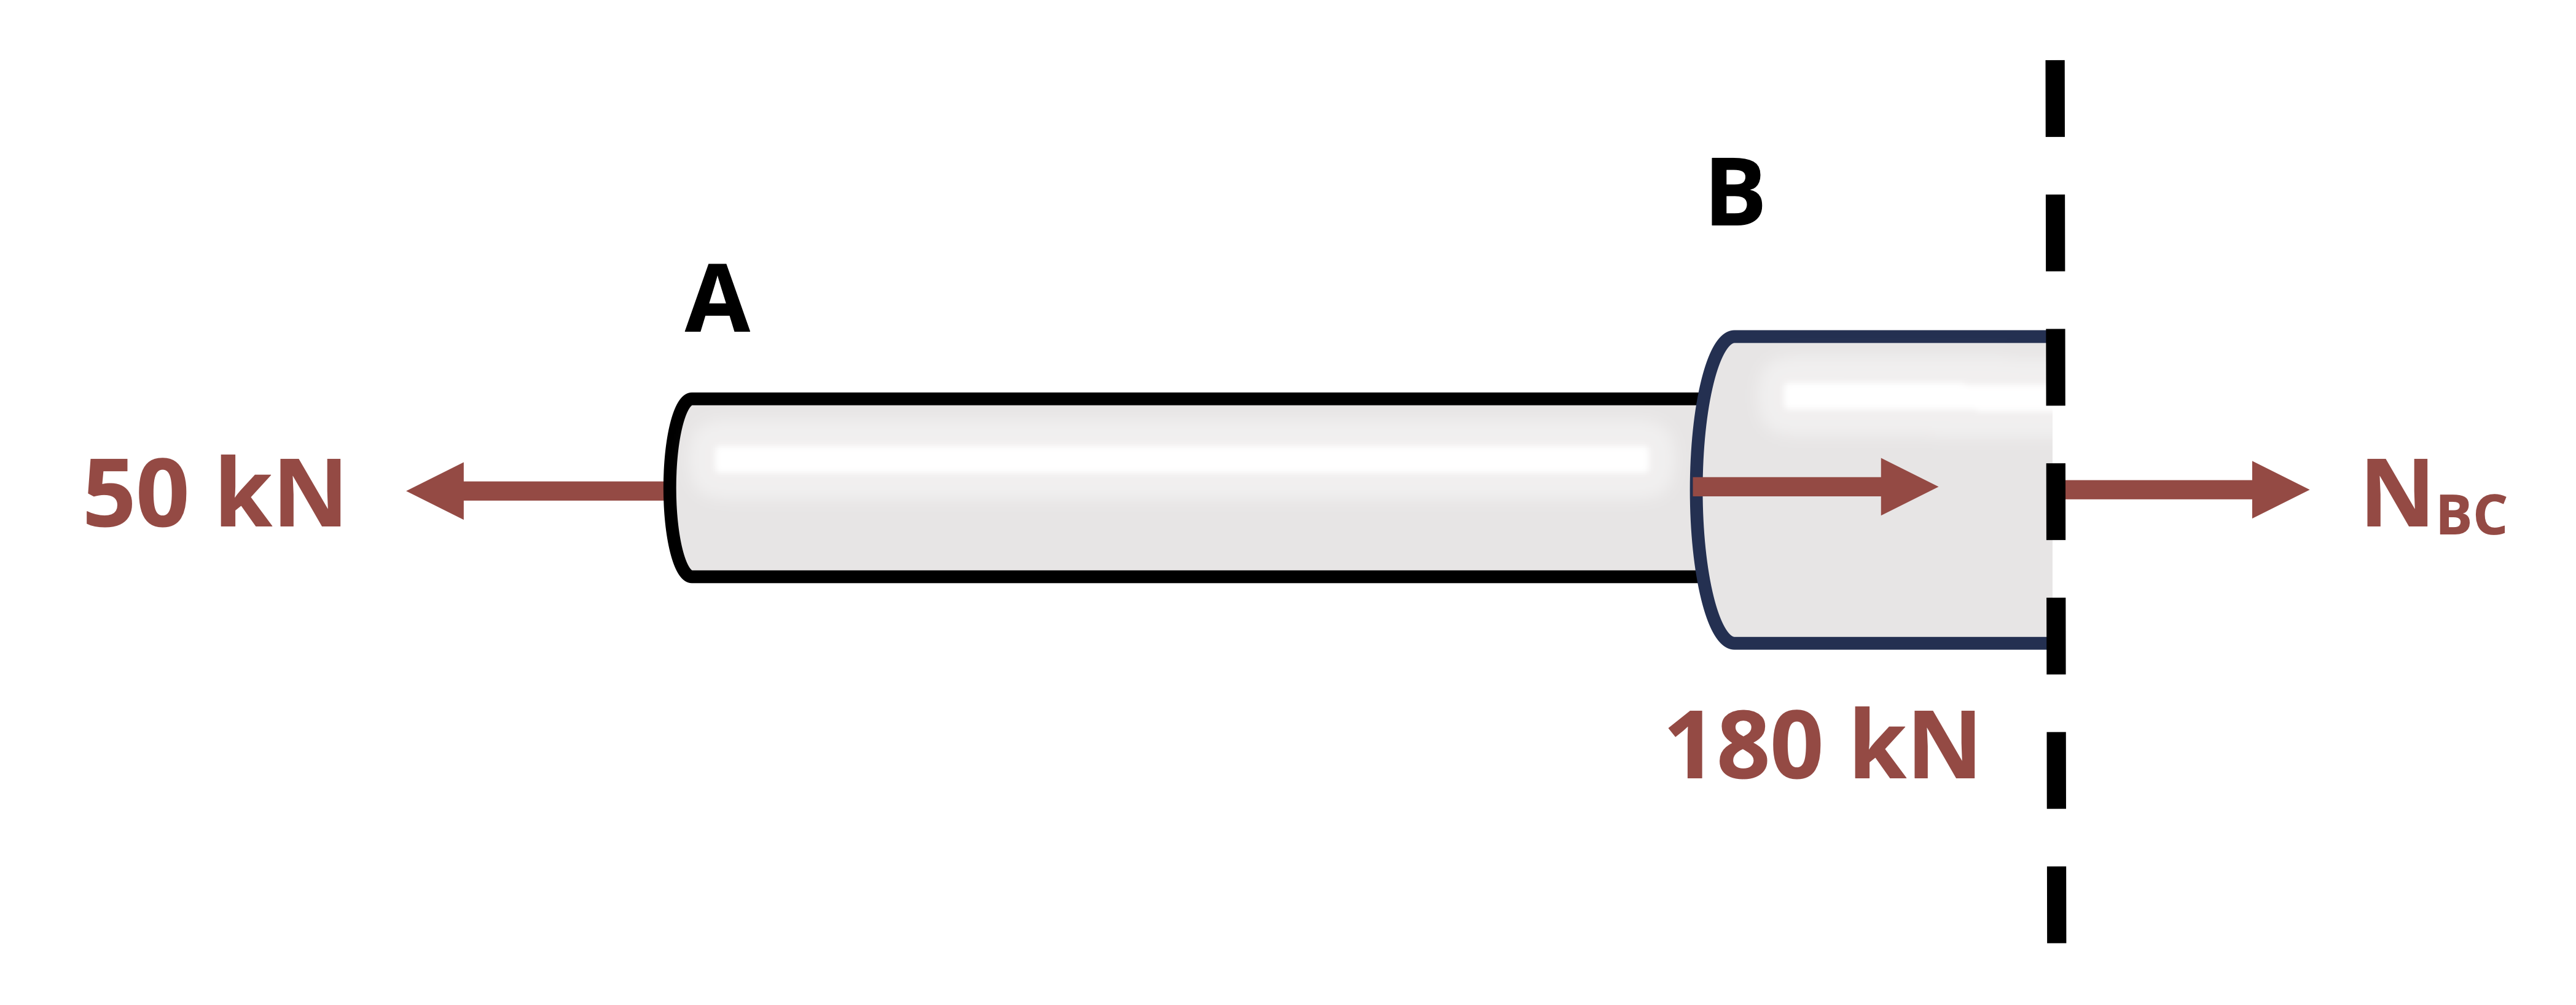
\includegraphics[width=3.15625in,height=\textheight]{images/Updated CH1 examples/example 1.5 part 3.png}
\end{center}

\[
\sum F_x=-50{~kN}+180{~kN}+N_{BC}=0 \quad\rightarrow\quad N_{BC}=-130{~kN}
\]

For both AB and BC, the internal normal force was assumed tensile in the
FBD and equilibrium equation. In the case of N\textsubscript{AB}, the
positive answer confirms that it is tensile. In the case of
N\textsubscript{BC}, the negative answer reveals that it is compressive.

\textbf{Answer: NAB = 50 kN (T), NBC = 130 kN (C)}

\end{tcolorbox}

\end{example}

\end{tcolorbox}

\section{Equilibrium and Reactions in Three Dimensions}\label{sec-1.3}

Click to expand

Because real life structures will be subject to forces and moments in
all directions, we will also see problems in which it will be necessary
to consider 3 dimensional forces and 3 dimensional moments.

For 3D systems, there are 6 total scalar equilibrium equations:

\begin{equation}\phantomsection\label{eq-1.2}{
\boxed{\begin{array}{ll}
\sum F_x=0 & \sum M_x=0 \\
\sum F_y=0 & \sum M_y=0 \\
\sum F_z=0 & \sum M_z=0
\end{array}}
}\end{equation}

Note that the moment vector describes the axis around which the body
tends to rotate. Each individual component represents the tendency of
the body to rotate around the specified axis. In 3D, there are three
internal forces and three internal moments (Figure~\ref{fig-1.3}). There
is one normal force (N\textsubscript{x}) perpendicular to the
cross-section and two shear forces (V\textsubscript{y} and
V\textsubscript{z}) parallel to the cross-section. There are two bending
moments (M\textsubscript{y} and M\textsubscript{z}) which act around the
axes parallel to the cross-section and one torsional moment
(T\textsubscript{x}) which acts around the axis perpendicular to the
cross-section. We will study each of these loads in detail over the next
few chapters.

\begin{figure}

\centering{

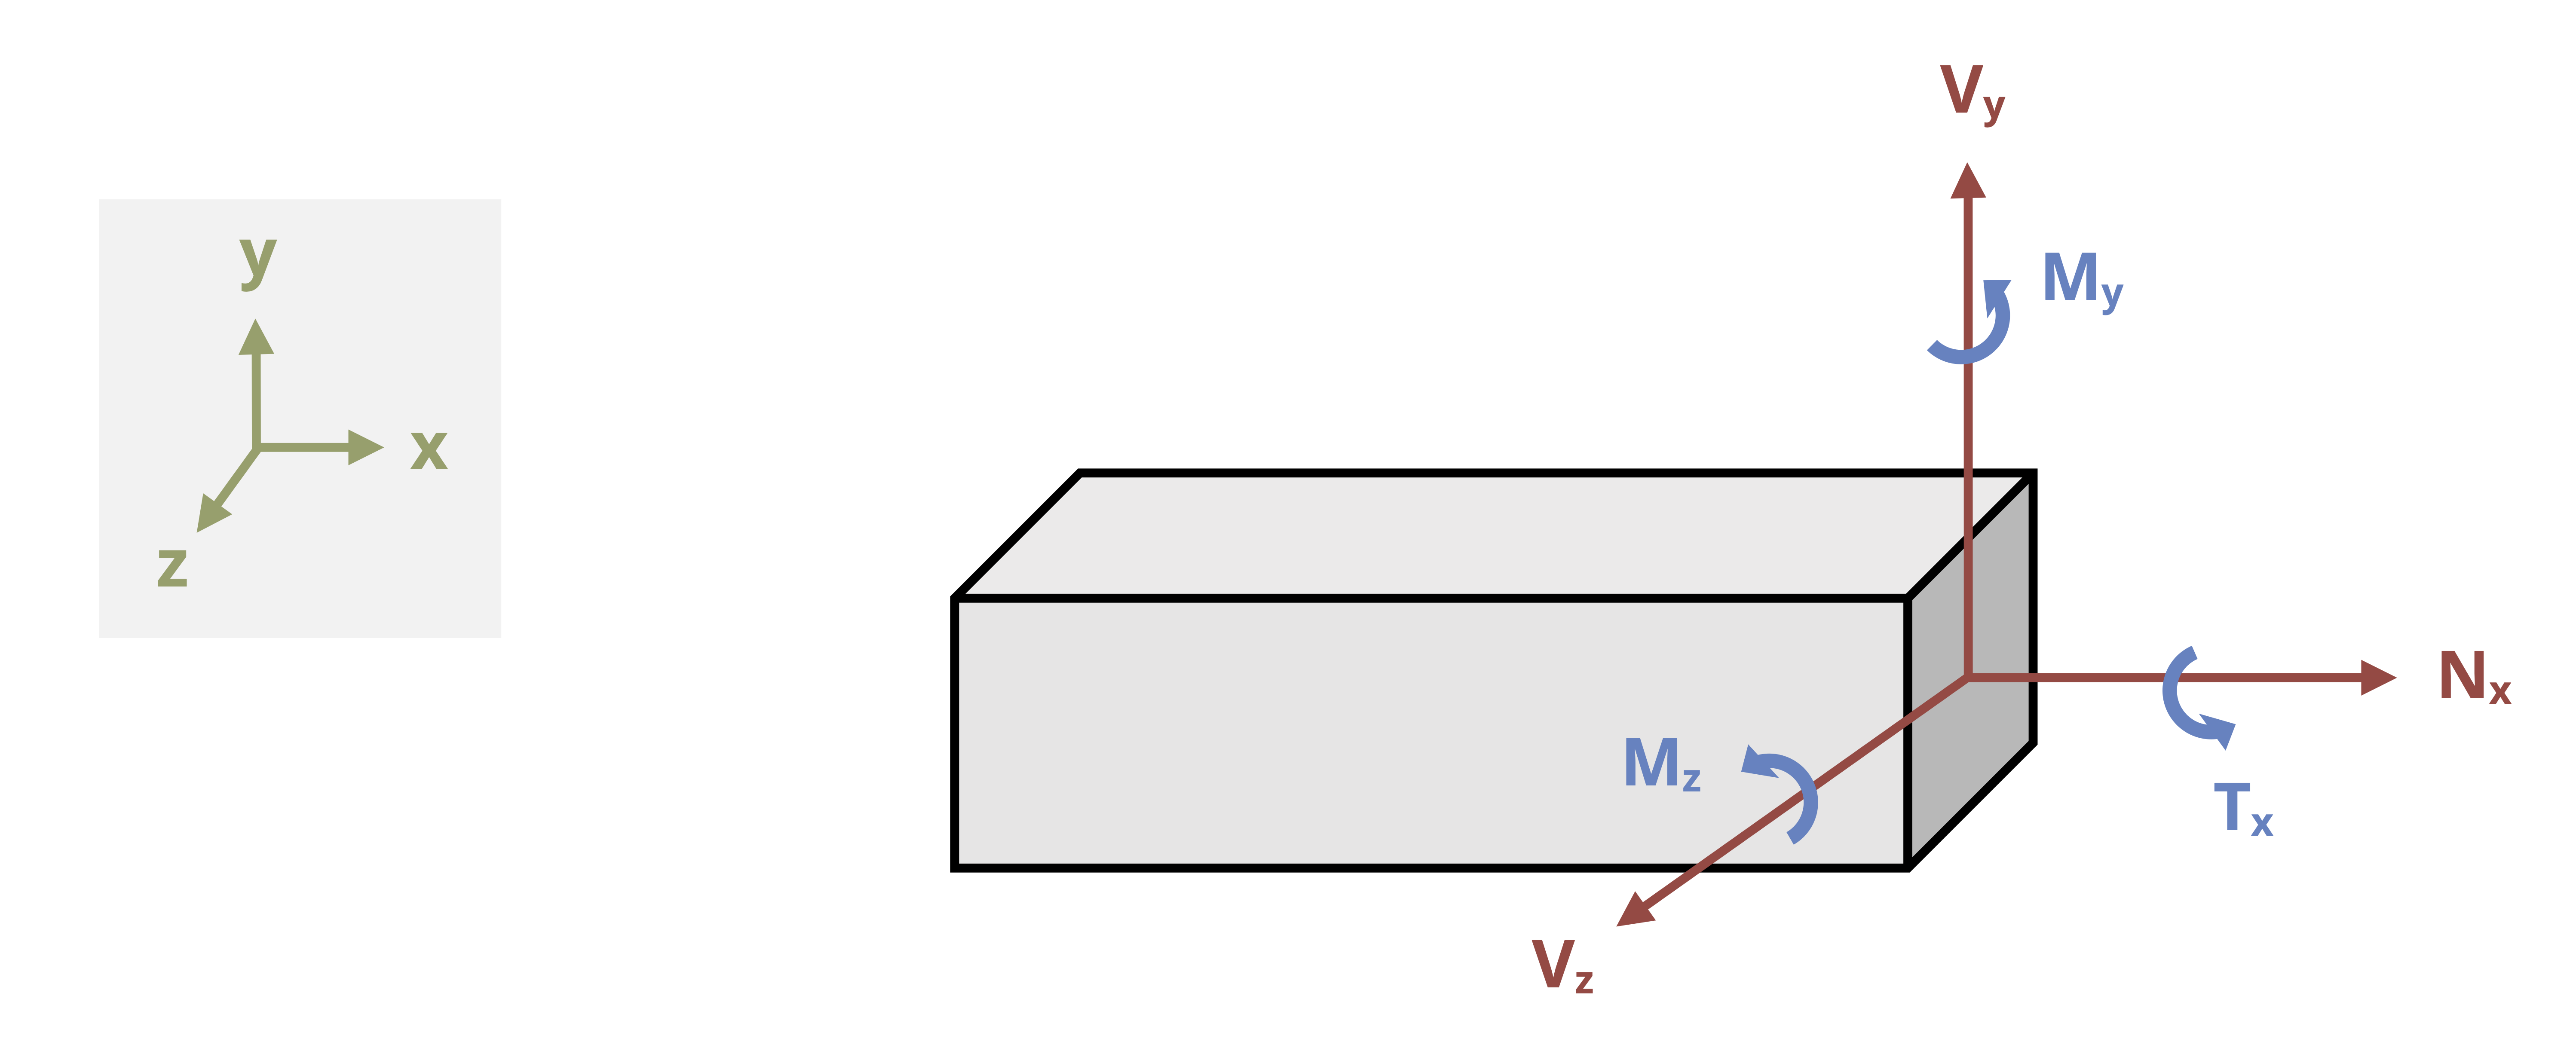
\includegraphics[width=5.3125in,height=\textheight]{images/CH1 PNGs/figure 1.3.png}

}

\caption{\label{fig-1.3}In 3D there are three internal forces (normal
force N\textsubscript{x} and two shear forces V\textsubscript{y} and
V\textsubscript{z}) and three internal moments (torsional moment
T\textsubscript{x} and two bending moments M\textsubscript{y} and
M\textsubscript{z})}

\end{figure}%

Note that the choice of coordinate system here is arbitrary. Loads are
defined as normal, shear, bending, or torsion based on how they act
relative to the cross-section. For example, the normal force may act in
the y-direction depending on how the cross-section is cut, and the
torsional moment would then act around the y-axis.

While summing the reaction forces in 3D is a straight-forward process of
adding forces in each direction, summing moments in 3D can prove to be
more complicated. To sum moments, there are generally two options. One
option is to use the cross product to calculate moments:
\(M=r \times F\)

In the cross-product equation, \textbf{r} is the position vector from
the point the moment is about to any point on the line of action of the
force. Using the cross product to calculate moment will result in a
vector expression for the moment equation that gives all three
components at one time with the correct signs to indicate clockwise
(negative) or counterclockwise (positive) rotation.

The second option to calculate moments is to perform scalar calculations
in which the sum of the moments about the x, y, and z axis is calculated
individually. To use this option, it might be helpful to recall:

\begin{enumerate}
\def\labelenumi{\arabic{enumi}.}
\item
  The general scalar equation for moment is M = F*d, where d is the
  perpendicular distance from the axis of rotation at the point the
  moment is being taken about to anywhere on the line of action of the
  force. One can also use M = F r sin α where r is the distance from the
  point to any point on the force and α is the angle between the
  position vector \textbf{r} (that corresponds to the magnitude r used)
  and the force vector.
\item
  Forces do not cause moments about points they go through or axes they
  act through.
\item
  Forces do not cause moments about axes they are parallel to (i.e.,
  F\textsubscript{x} wouldn't cause a moment around an x-axis no matter
  where the point is).
\item
  When taking the moment about a point, the origin of the coordinate
  axes should be moved to that point for the purpose of determining the
  distance between the axis and the force.
\end{enumerate}

Given all the reminders above, one can apply the following equations:

\(\sum M_x= \pm F_y * z \pm F_z * y\) where z and y are the respective
distances from the x-axis at the point in question to F\textsubscript{y}
and F\textsubscript{z} components of the force respectively.

\(\sum M_y= \pm F_x * z \pm F_z * x\) where z and x are the respective
distances from the y-axis at the point in question to F\textsubscript{x}
and F\textsubscript{z} components of the force respectively.

\(\sum M_z= \pm F_x * y \pm F_y * x\) where y and x are the respective
distances from the z-axis at the point in question to the
F\textsubscript{x} and F\textsubscript{y} components of the force
respectively.

The ± is decided based on the right-hand rule (see text below for
guidance) or visual inspection. When using visual inspection, the
direction of rotation is judged by looking from the positive end of the
axis towards the negative end. A counterclockwise rotation is considered
to be positive and a clockwise rotation is considered to be negative.

To apply the right-hand rule:

\begin{enumerate}
\def\labelenumi{\arabic{enumi}.}
\item
  Orient your right hand so that the fingers are aligned with the moment
  arm with the palm at the point and the fingertips extending towards
  the force. The moment arm is the axis along which the perpendicular
  distance to the axis would be determined. For example, if finding
  M\textsubscript{x} due to F\textsubscript{y}, the moment arm is in the
  z direction.
\item
  The thumb is aligned with the axis of rotation (axis around which the
  moment is being calculated).
\item
  Curl your fingers in the direction of the force. If your thumb must be
  pointed in the positive axis direction to perform this action, the
  moment is counterclockwise. If your thumb must be pointed in the
  negative axis direction, the moment is clockwise. Typical convention
  designates counterclockwise rotation to be positive and clockwise to
  be negative.
\end{enumerate}

These concepts are further reviewed in Example~\ref{exm-1.6}.

\begin{tcolorbox}[enhanced jigsaw, colback=white, colframe=quarto-callout-tip-color-frame, toptitle=1mm, arc=.35mm, bottomrule=.15mm, toprule=.15mm, opacitybacktitle=0.6, title={Example 1.6}, coltitle=black, breakable, colbacktitle=quarto-callout-tip-color!10!white, bottomtitle=1mm, titlerule=0mm, opacityback=0, leftrule=.75mm, left=2mm, rightrule=.15mm]

\begin{example}[]\protect\hypertarget{exm-1.6}{}\label{exm-1.6}

~

Determine the internal reactions at point P, located at the center of
the cross-section of the rectangular bar and 1.75 ft from the fixed
support, if \textbf{F} = -150\textbf{i} - 225\textbf{j} + Fz =
300\textbf{k} lb.

\begin{center}
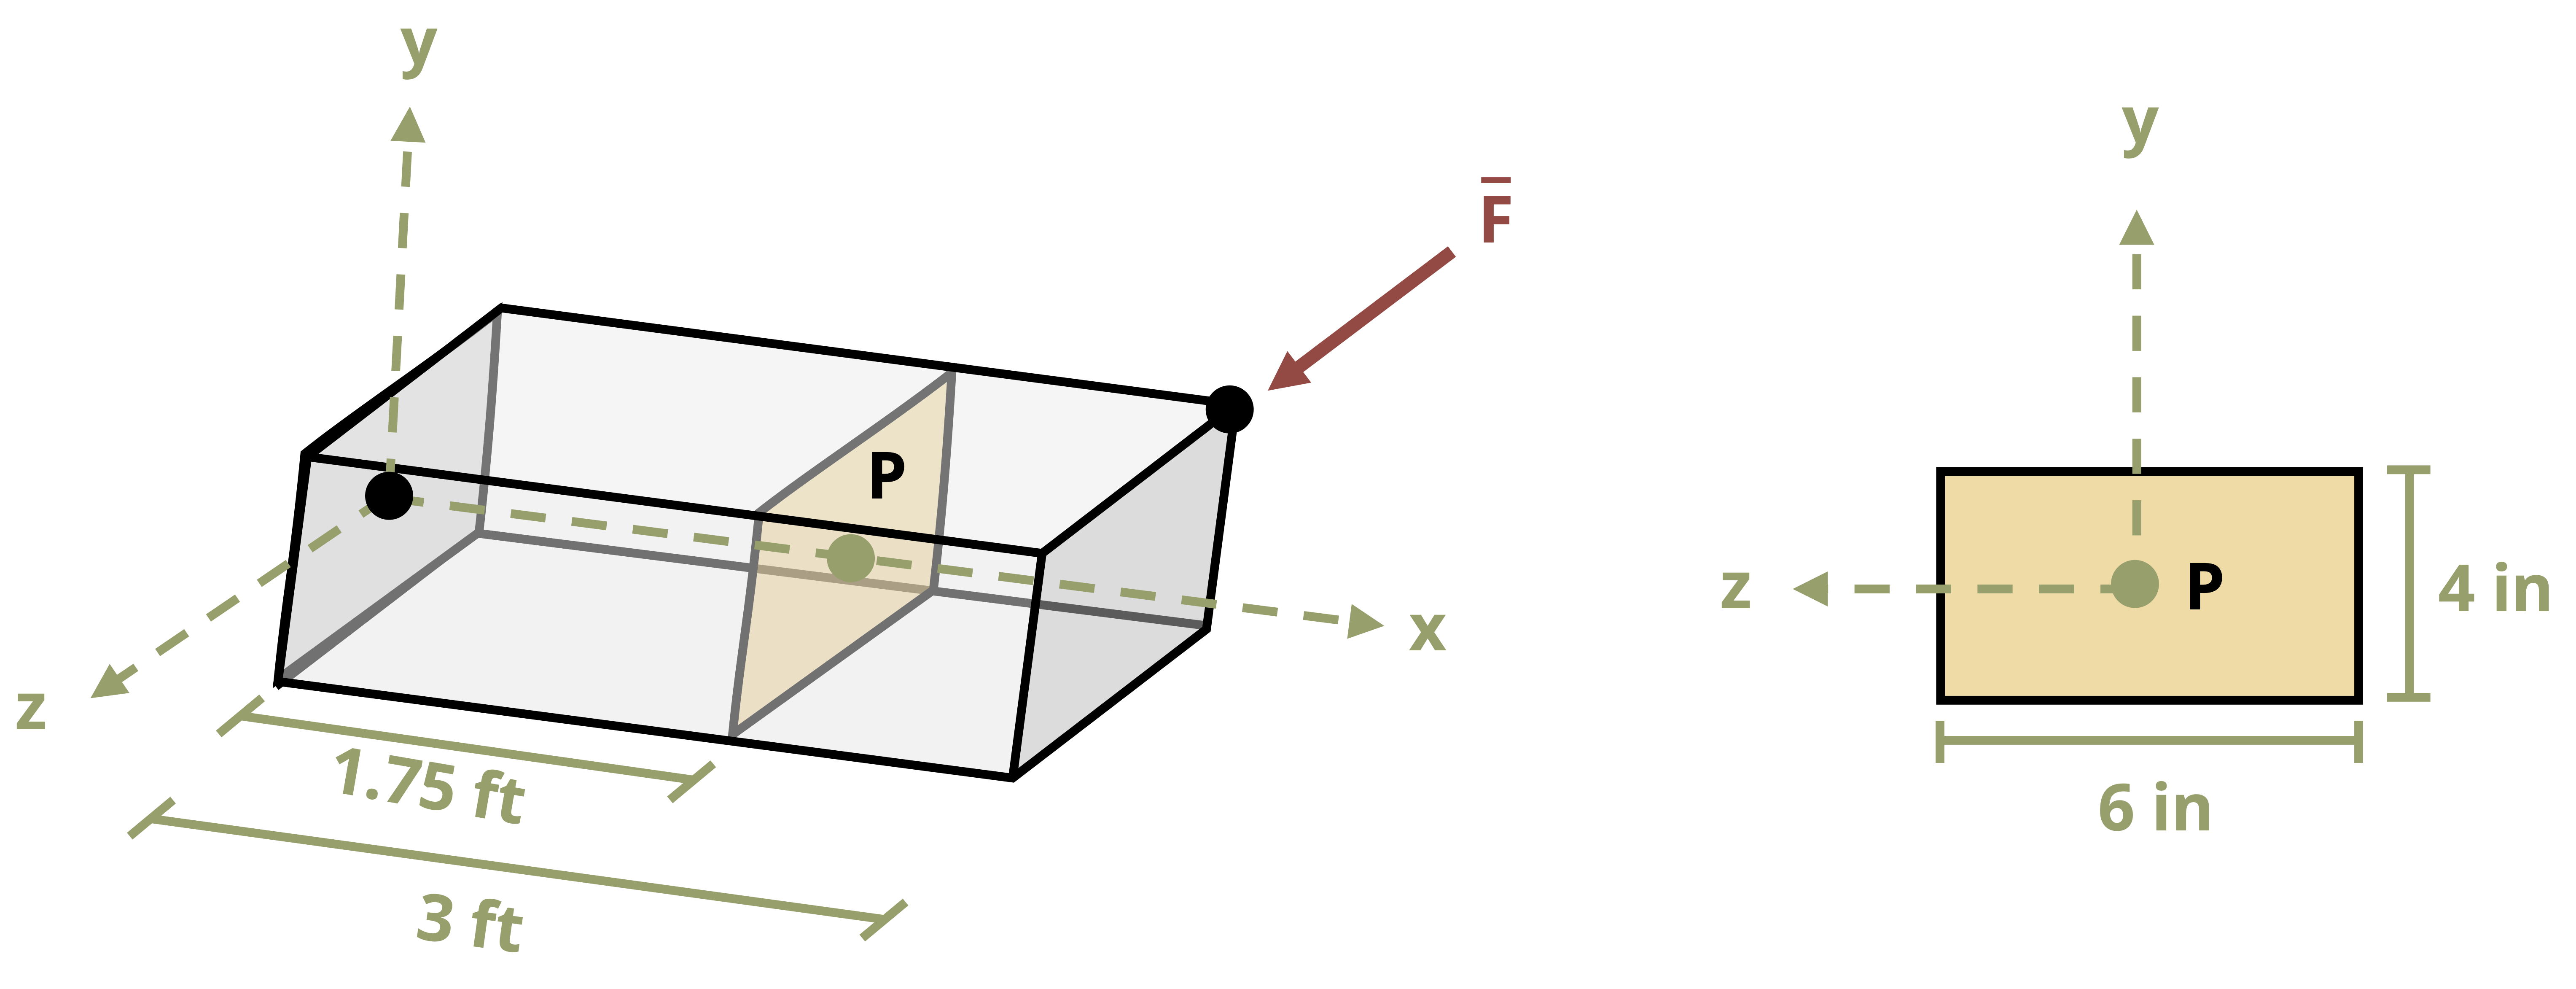
\includegraphics[width=5.04167in,height=\textheight]{images/CH1 PNGs/example 1.6 part 1.png}
\end{center}

\begin{tcolorbox}[enhanced jigsaw, colback=white, colframe=quarto-callout-tip-color-frame, toptitle=1mm, arc=.35mm, bottomrule=.15mm, toprule=.15mm, opacitybacktitle=0.6, title={Solution}, coltitle=black, breakable, colbacktitle=quarto-callout-tip-color!10!white, bottomtitle=1mm, titlerule=0mm, opacityback=0, leftrule=.75mm, left=2mm, rightrule=.15mm]

To determine the internal reactions at P, a cut is made at P that is
parallel to the cross section. Since the left side of the cut would
include the wall but the right side of the cut would be free with no
external reactions to determine, the right side section will be used.

\begin{center}
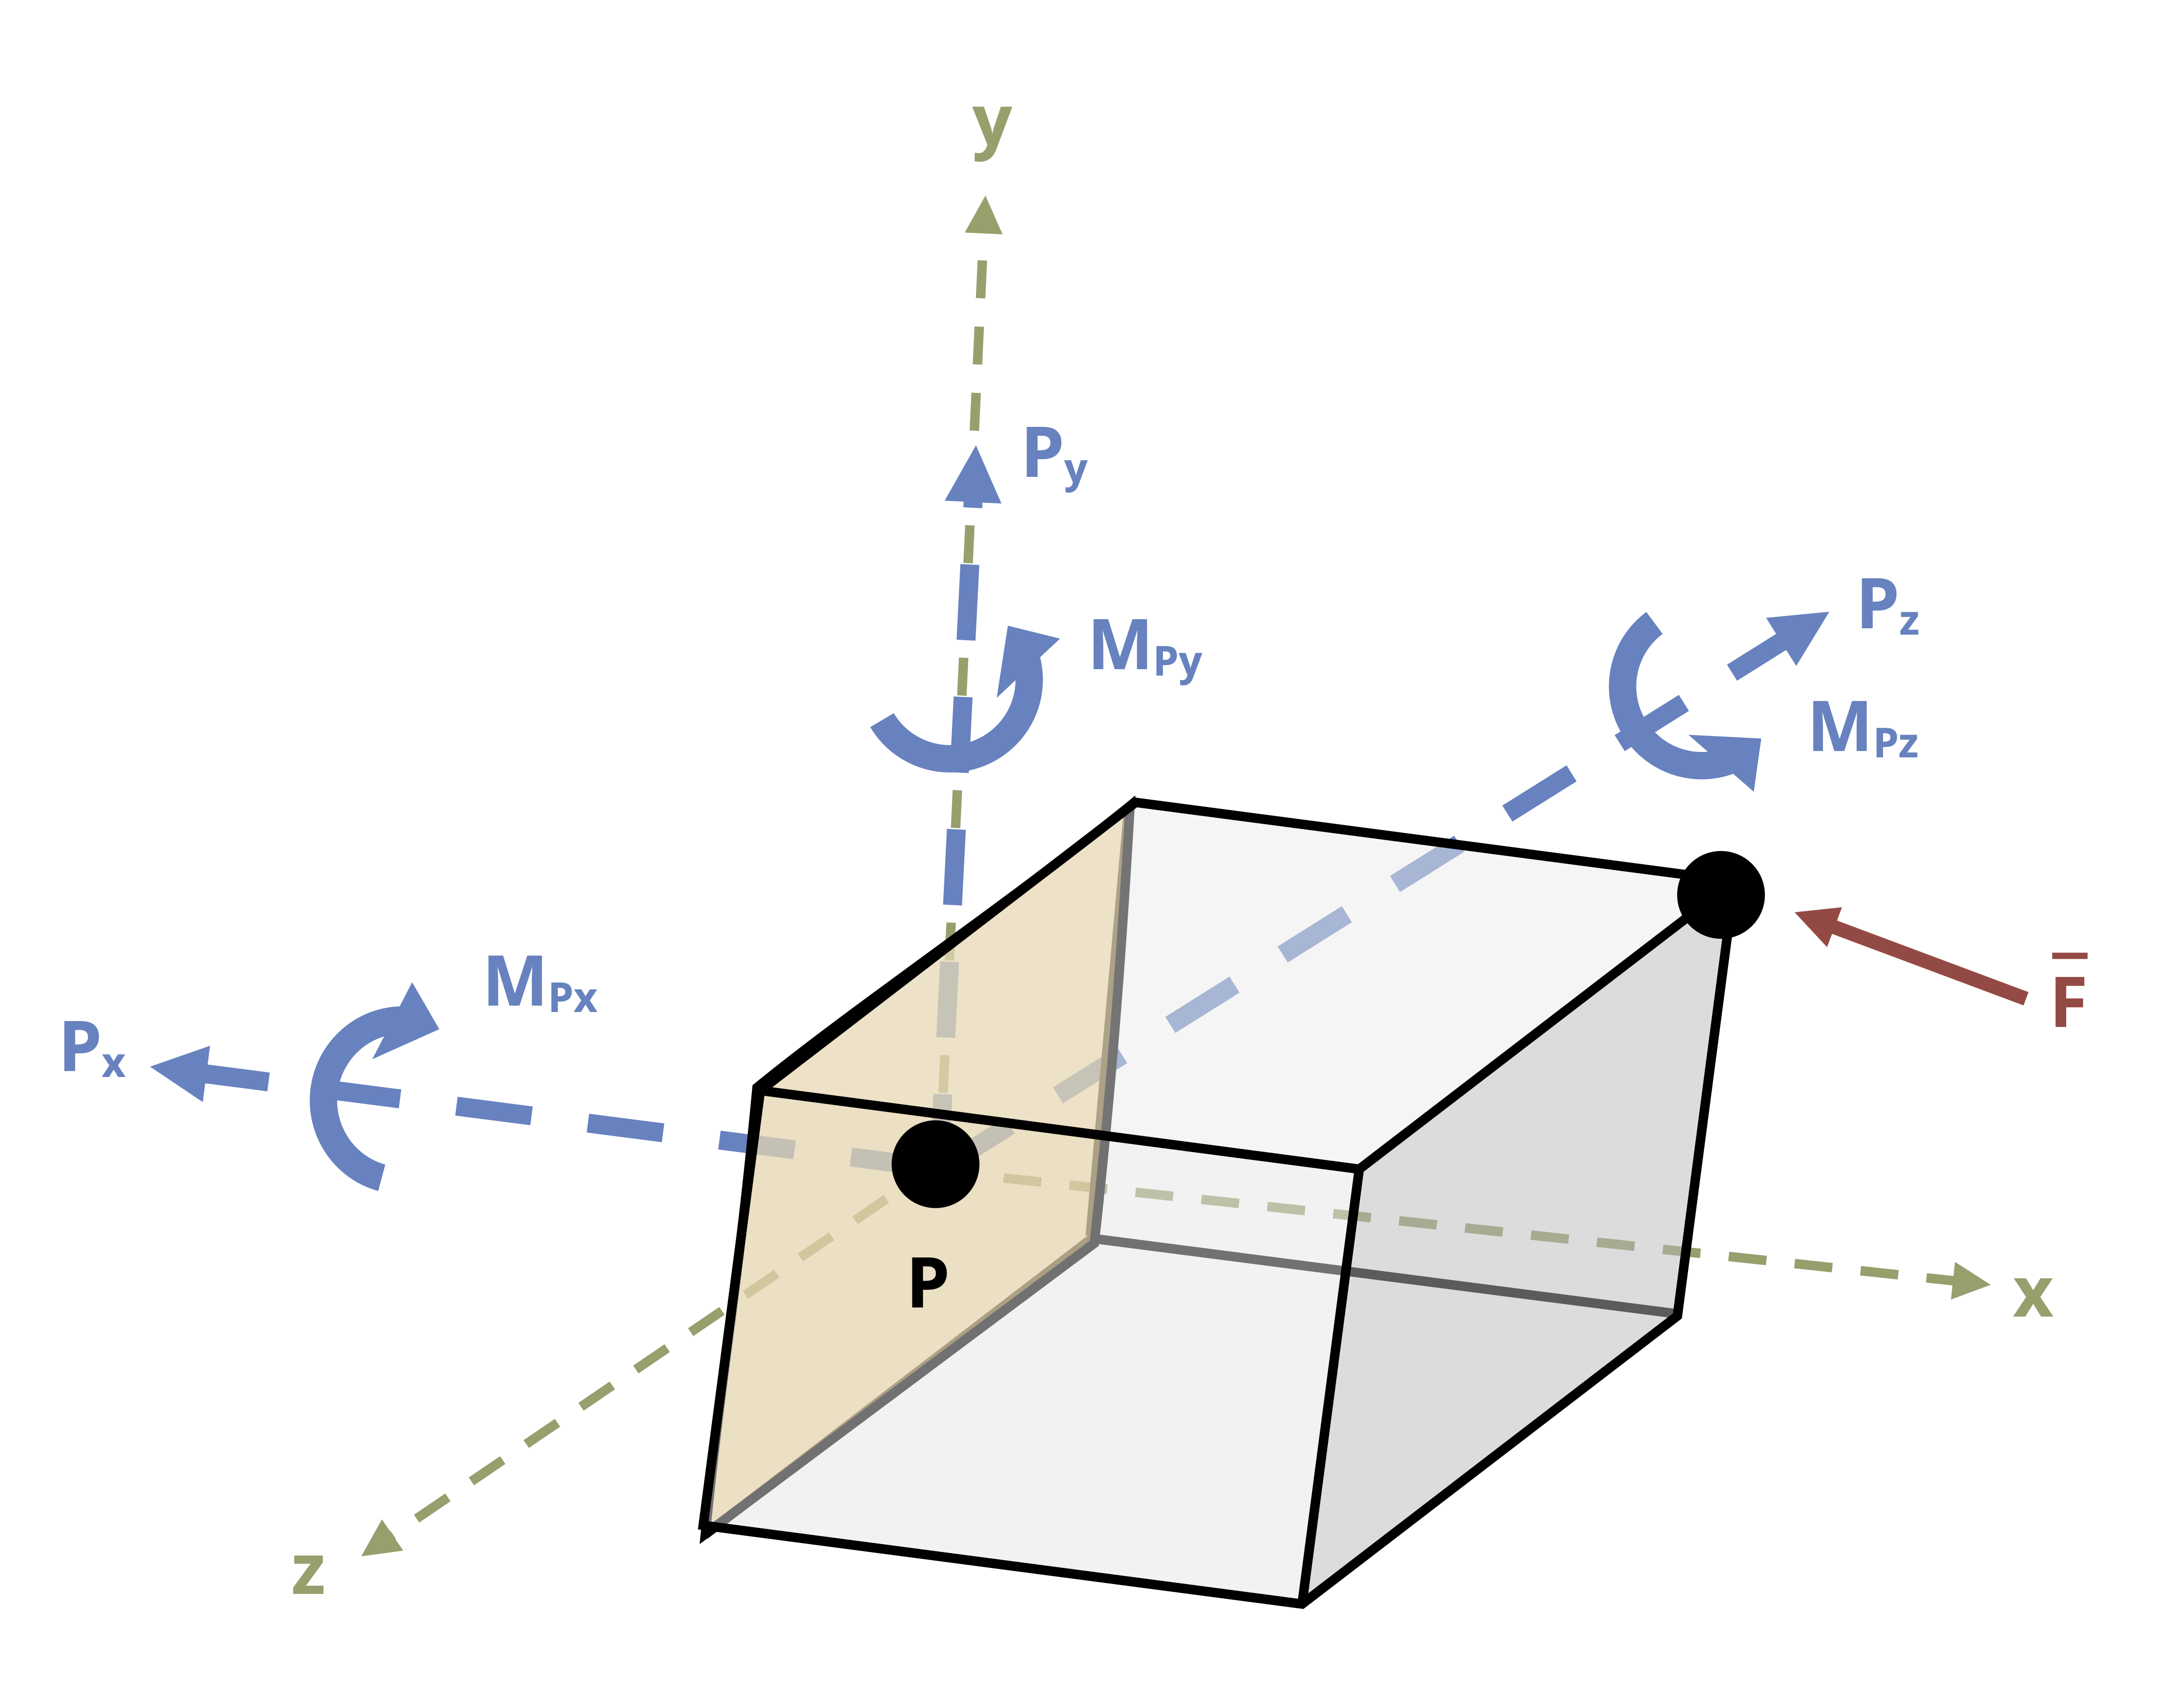
\includegraphics[width=4.04167in,height=\textheight]{images/CH1 PNGs/example 1.6 part 2.png}
\end{center}

The force reactions at P will just be equal (but opposite in direction)
to the force shown since there is only one. The moment reactions can be
found by taking the moments about point P.

The moment about the x axis at point P is:

\[
\sum M_{Px} = \pm ~F_yz \pm F_zy = 0 = -[(225{~lb})(3{~in})(\frac{1{~ft}}{12{~in}})]+[(300{~lb})(2{~in})(\frac{1{~ft}}{12{~in}})]+M_{px} -6.25{~lb·ft}
\]

The moment about the y axis at point P is:

\[
\sum M_{Py} = \pm ~F_xz \pm F_zx = 0 = -[(150{~lb})(3{~in})(\frac{1{~ft}}{12{~in}})]-[(300{~lb})(1.25{~ft})]+M_{py} -347.5{~lb·ft}
\]

The moment about the z axis at point P is:

\[
\sum M_{Pz} = \pm F_xy \pm F_yx = 0 = [(150{~lb})(2{~in})(\frac{1{~ft}}{12{~in}})]-[(225{~lb})(1.25{~ft})]+M_{pz} -2.5{~lb·ft}
\]

The sign on the individual multiplicative terms in each equation are
determined by right hand rule or visualization.

\textbf{Answer:}

P\textsubscript{x} = 150 lb

P\textsubscript{y} = 225 lb

P\textsubscript{z} = 300 lb

M\textsubscript{Px} = 6.25 lb·ft

M\textsubscript{Py} = 348 lb·ft

M\textsubscript{Pz} = 2.5 lb·ft

\end{tcolorbox}

\end{example}

\end{tcolorbox}

\section*{Summary}\label{summary}
\addcontentsline{toc}{section}{Summary}

\markright{Summary}

Click to expand

\begin{tcolorbox}[enhanced jigsaw, colback=white, colframe=quarto-callout-note-color-frame, toptitle=1mm, arc=.35mm, bottomrule=.15mm, toprule=.15mm, opacitybacktitle=0.6, title={Key takeaways}, coltitle=black, breakable, colbacktitle=quarto-callout-note-color!10!white, bottomtitle=1mm, titlerule=0mm, opacityback=0, leftrule=.75mm, left=2mm, rightrule=.15mm]

Bodies in this text are in static equilibrium and subjected to external
forces and moments. Reaction forces and moments at supports can be
determined in 2D and 3D through equilibrium equations, just like in
Statics.

Unlike Statics, bodies in this course are deformable. We must also
determine internal loads. These can be found by cutting a cross-section
at the point of interest and again applying equilibrium equations.

In 2D there are two internal forces and one internal moment:

\begin{itemize}
\item
  Normal force (N) perpendicular to the cross-section
\item
  Shear force (V) parallel to the cross-section
\item
  Bending moment (M)
\end{itemize}

In 3D there are three internal forces and three internal moments:

\begin{itemize}
\item
  Normal force (N) perpendicular to the cross-section
\item
  Two shear forces (V) parallel to the cross-section
\item
  Torsional moment (T) acting around the axis perpendicular to the
  cross-section
\item
  Two bending moments (M) acting around the axes parallel to the
  cross-section
\end{itemize}

The effects of these internal loads on deformable bodies is the focus of
this text.

\end{tcolorbox}

\begin{tcolorbox}[enhanced jigsaw, colback=white, colframe=quarto-callout-note-color-frame, toptitle=1mm, arc=.35mm, bottomrule=.15mm, toprule=.15mm, opacitybacktitle=0.6, title={Key equations}, coltitle=black, breakable, colbacktitle=quarto-callout-note-color!10!white, bottomtitle=1mm, titlerule=0mm, opacityback=0, leftrule=.75mm, left=2mm, rightrule=.15mm]

Static equilibrium:

\[
\begin{array}{ll}
\sum F_x=0 & \sum M_x=0 \\
\sum F_y=0 & \sum M_y=0 \\
\sum F_z=0 & \sum M_z=0
\end{array}
\]

\end{tcolorbox}

\bookmarksetup{startatroot}

\chapter{Stress}\label{sec-stress}

\begin{tcolorbox}[enhanced jigsaw, colback=white, colframe=quarto-callout-note-color-frame, toptitle=1mm, arc=.35mm, bottomrule=.15mm, toprule=.15mm, opacitybacktitle=0.6, title={Learning Objectives}, coltitle=black, breakable, colbacktitle=quarto-callout-note-color!10!white, bottomtitle=1mm, titlerule=0mm, opacityback=0, leftrule=.75mm, left=2mm, rightrule=.15mm]

\begin{itemize}
\tightlist
\item
  Use internal loads to calculate average normal stress
\item
  Use internal loads to calculate average shear stress
\item
  Use the loads between surfaces to calculate bearing stress
\item
  Calculate stresses on inclined planes
\end{itemize}

\end{tcolorbox}

\section*{Introduction}\label{introduction-1}
\addcontentsline{toc}{section}{Introduction}

\markright{Introduction}

Click to expand

Having reviewed static equilibrium in Chapter~\ref{sec-statics}, we now
know how to find the internal loads in a body using equilibrium. When
determining whether a body can resist the loads applied to it, the
internal load is only part of the solution. The dimensions of the body
and the inherent properties of the material it is made from are also
important.

In this chapter we'll explore the concept of stress, which can help us
determine whether an object will physically break when subjected to a
load. We'll cover average normal stress (stress perpendicular to the
cross-section) in Section~\ref{sec-2.1} and average shear stress (stress
parallel to the cross-section) in Section~\ref{sec-2.2}. We'll then
discuss bearing stress (the stress between two bodies in contact with
each other) in Section~\ref{sec-2.3} and finish with the average normal
and shear stresses on an inclined cross-section in
Section~\ref{sec-2.4}.

\section{Average Normal Stress}\label{sec-2.1}

Click to expand

Average normal stress is defined as the internal normal force divided by
the cross-sectional area of the body. It is given the Greek letter sigma
(σ). Stress increases as the force increases or as the cross-sectional
area decreases.

\begin{equation}\phantomsection\label{eq-2.1}{
\boxed
{\sigma=\frac{N}{A}}
}\end{equation}

\emph{where}\\
\emph{𝜎 = Average normal stress {[}Pa, psi{]}}\\
\emph{N = Internal normal force {[}N, lb{]}}\\
\emph{A = Cross-sectional area {[}m\textsuperscript{2},
in.\textsuperscript{2}{]}}

As such the SI units of stress are N/m\textsuperscript{2}, more commonly
referred to as the Pascal (Pa) where 1 Pa = 1 N/m\textsuperscript{2}.
The US customary units for stress are lb/in\textsuperscript{2}, commonly
written as psi. Since stresses can get very large, it is common to use
prefixes such as kilo (k) and mega (M) to represent
10\textsuperscript{3} and 10\textsuperscript{6} respectively. A stress
of 15,000,000 Pa is written as 15 MPa. A stress of 35,000 psi is written
as 35 ksi.

Normal stress occurs perpendicular to the cross-section and so is
associated with either a pulling or pushing motion
(Figure~\ref{fig-2.1}). Normal forces that pull on a cross-section are
known as tensile forces and create a tensile normal stress. Normal
forces that push on a cross-section are known as compressive forces and
create a compressive normal stress. The normal stress calculated above
is really an average normal stress as the force is distributed over the
cross-section, but we generally simplify this to a concentrated force
that creates the same normal stress at every point on the cross-section
(Figure~\ref{fig-2.2}).

\begin{figure}

\centering{

\includegraphics{images/CH2 figures/2.1.png}

}

\caption{\label{fig-2.1}Forces pulling on a cross-section cause tension,
while forces pushing on a cross-section cause compression. Both are very
common. Left: A crane cable during a lift experiences tension. Right:
The support columns under a bridge experience compression.}

\end{figure}%

\begin{figure}

\centering{

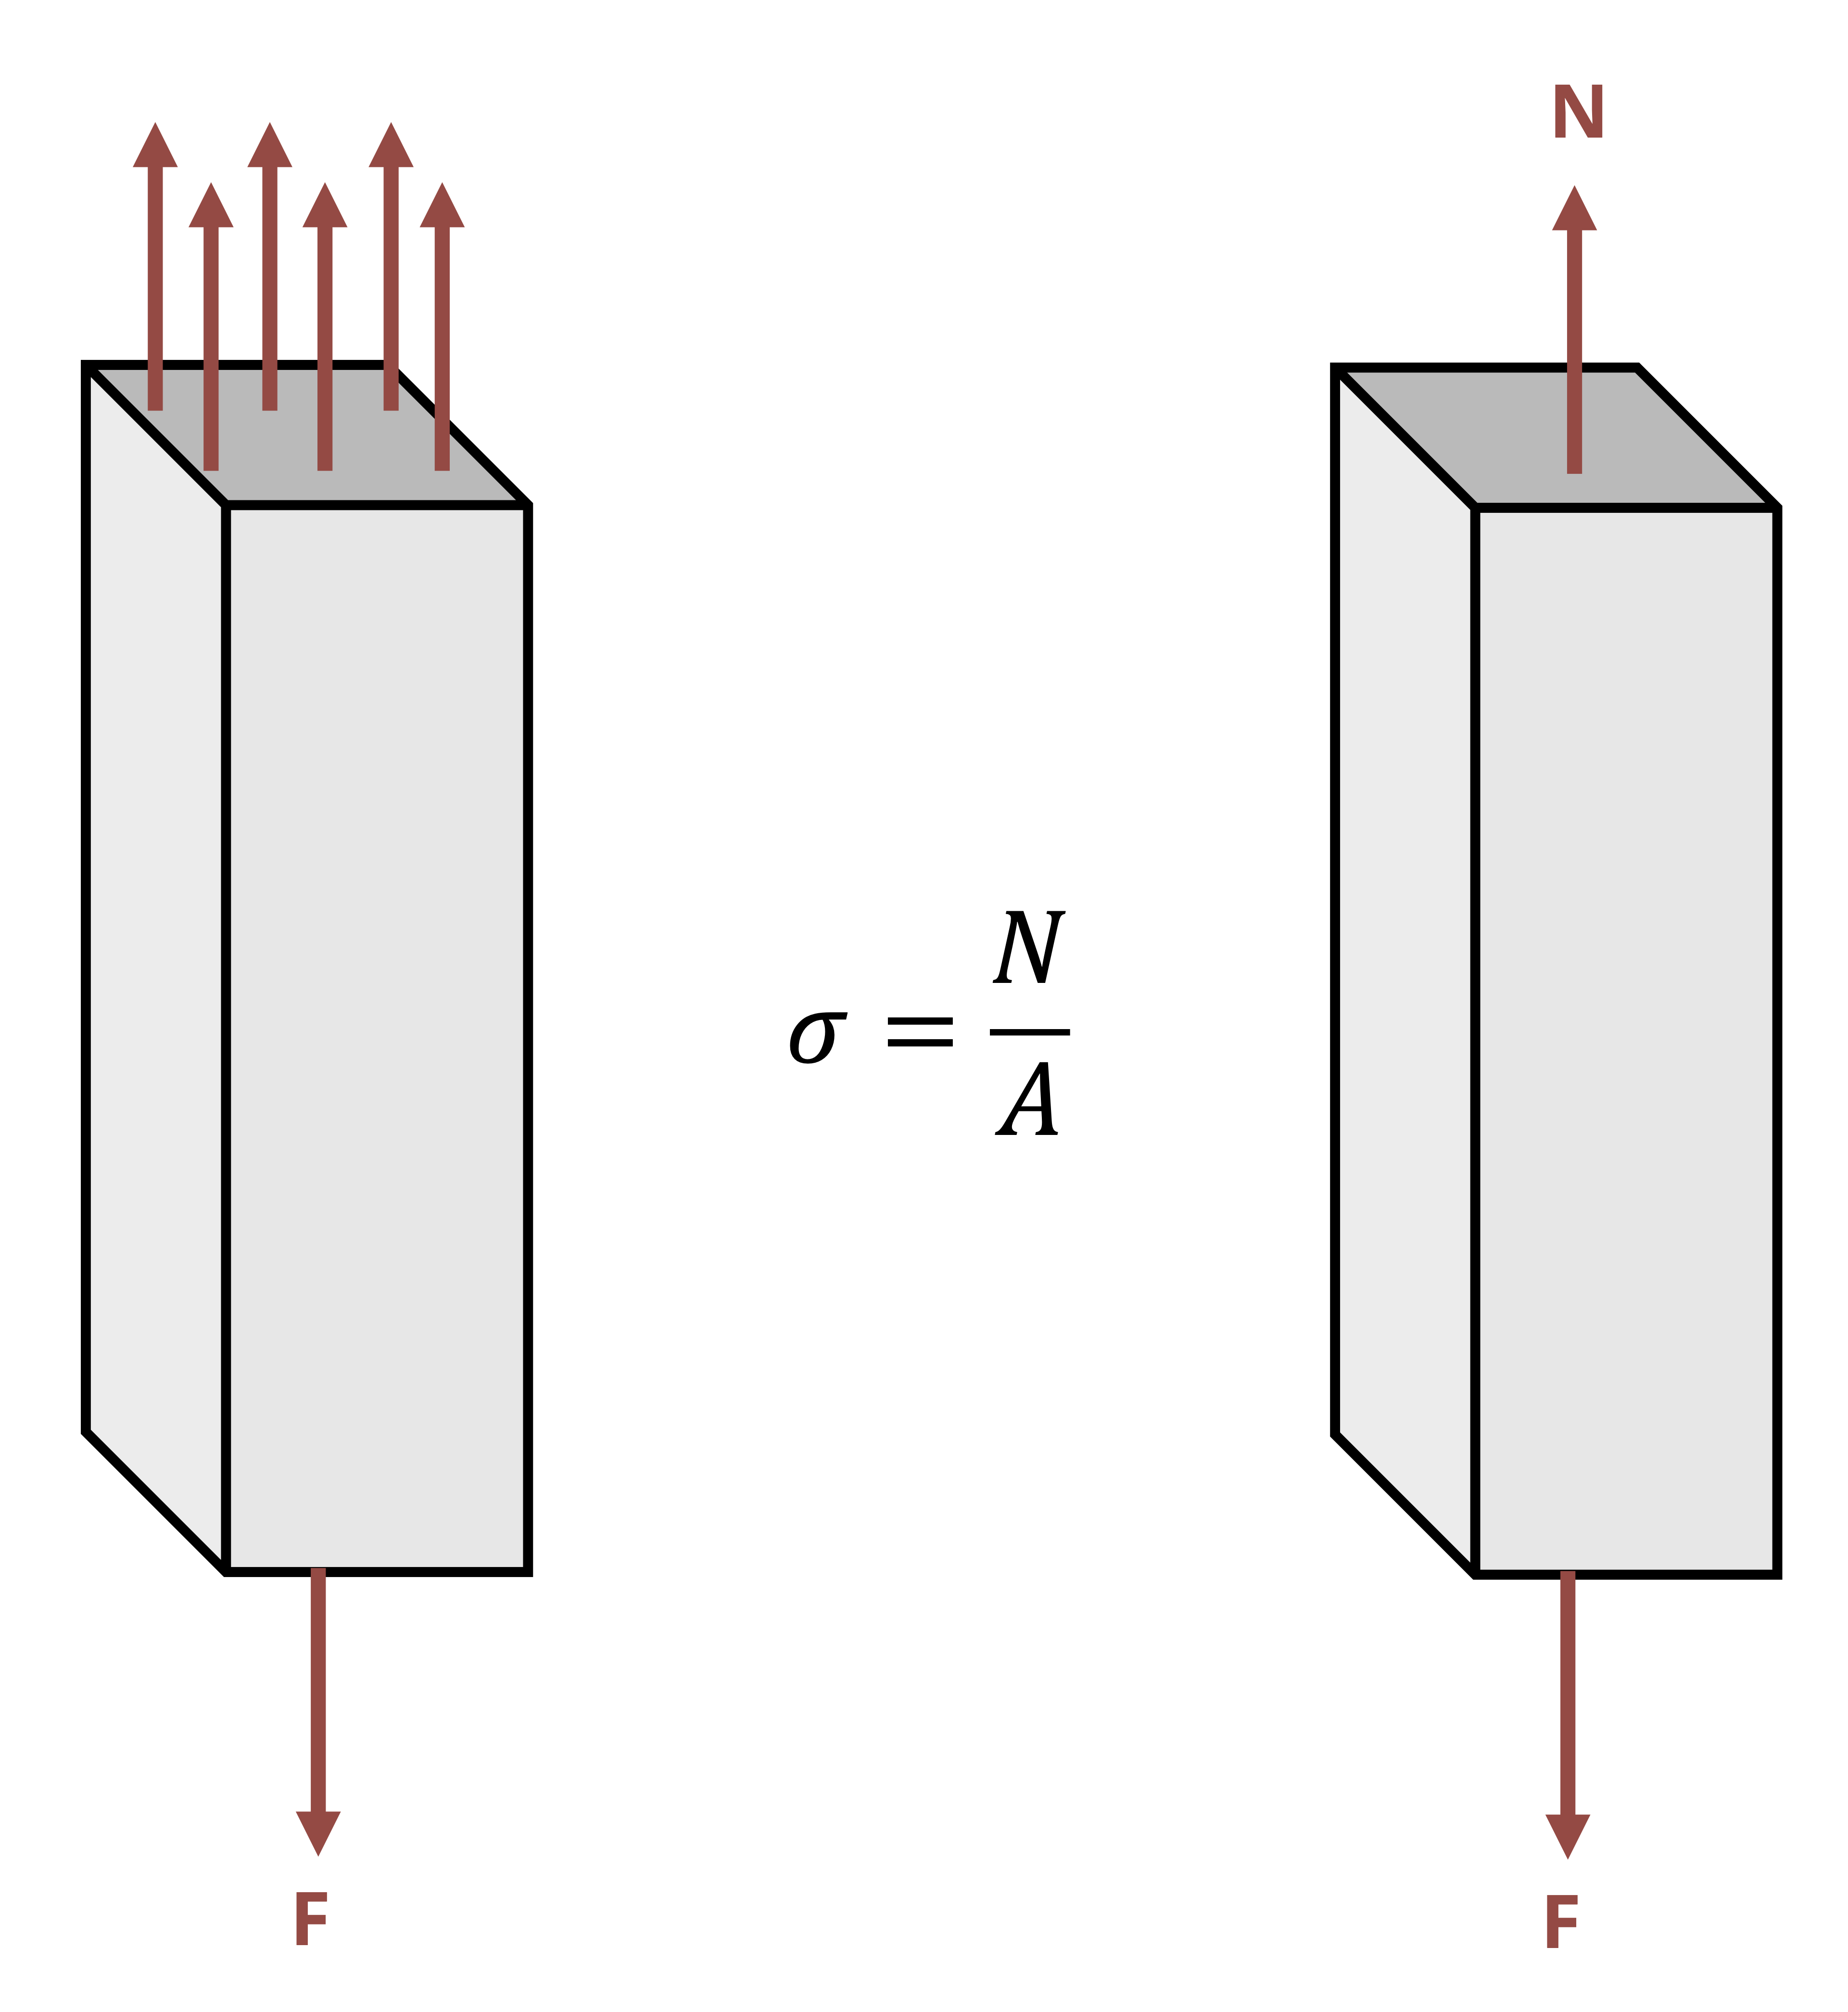
\includegraphics{images/CH2 figures/2.2.png}

}

\caption{\label{fig-2.2}The internal load is equally distributed over
the cross-sectional area, but may be represented as a single
concentrated load acting at the center (N in this case). The stress is
therefore an average normal stress.}

\end{figure}%

The internal normal force in a body can be found through the method of
equilibrium as reviewed in Section~\ref{sec-1.2}. See
Example~\ref{exm-2.1} for a demonstration.

\begin{tcolorbox}[enhanced jigsaw, colback=white, colframe=quarto-callout-tip-color-frame, toptitle=1mm, arc=.35mm, bottomrule=.15mm, toprule=.15mm, opacitybacktitle=0.6, title={Example 2.1}, coltitle=black, breakable, colbacktitle=quarto-callout-tip-color!10!white, bottomtitle=1mm, titlerule=0mm, opacityback=0, leftrule=.75mm, left=2mm, rightrule=.15mm]

\begin{example}[]\protect\hypertarget{exm-2.1}{}\label{exm-2.1}

~

The support column will be subjected to a compressive force F = 65 kips.

\begin{center}
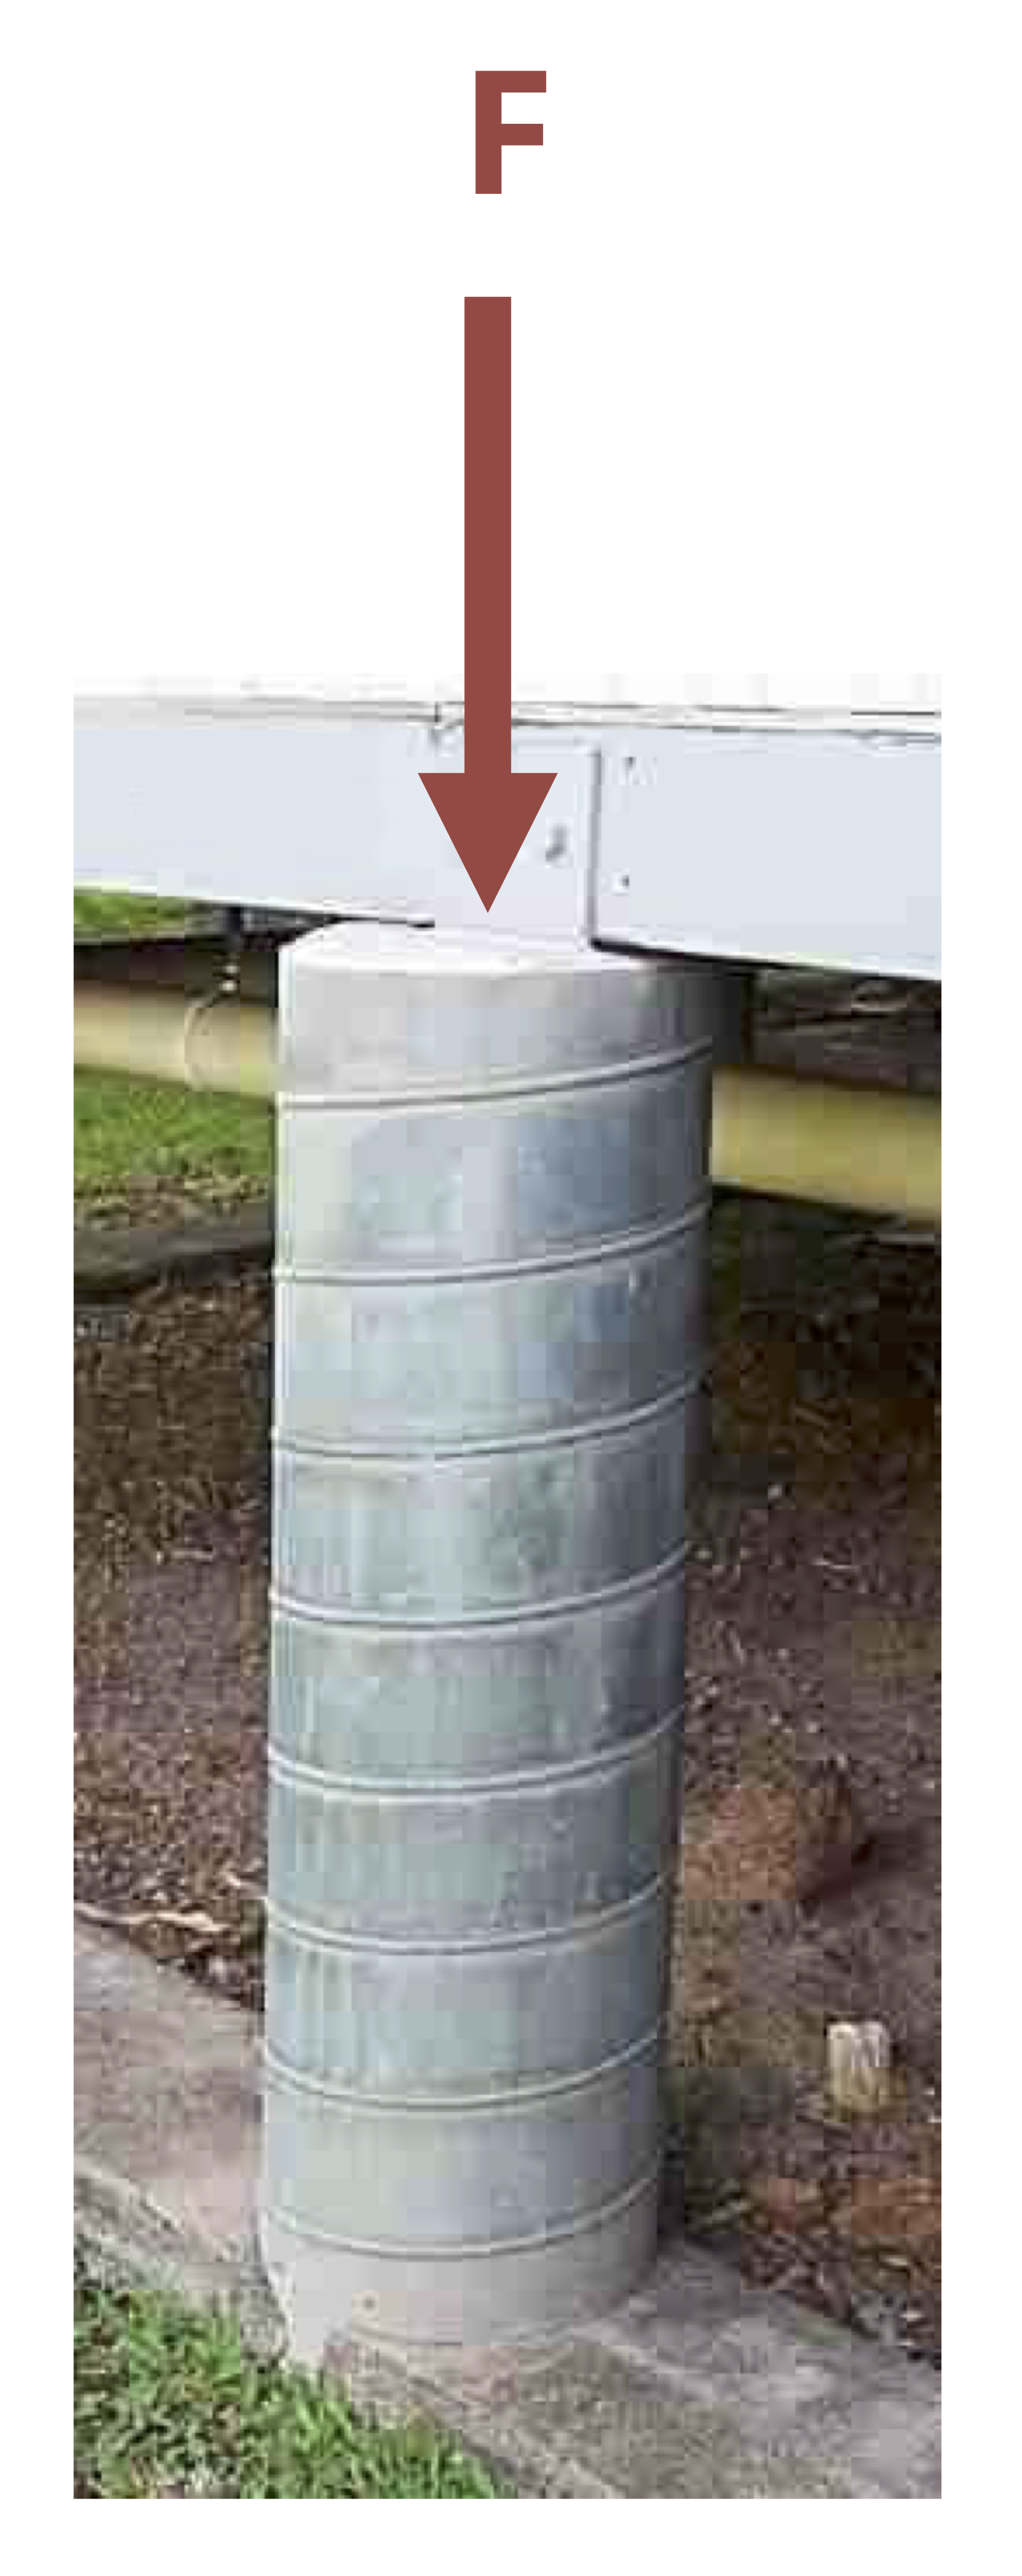
\includegraphics[width=1.8125in,height=\textheight]{images/Updated CH2 examples/example 2.1 part 1.png}
\end{center}

\begin{enumerate}
\def\labelenumi{\arabic{enumi}.}
\item
  The diameter of the column is 4 inches. Determine the average normal
  stress in the column.
\item
  The column is to be made of concrete with an allowable compressive
  stress of 4 ksi. For the same force F = 65 kips, determine the
  required diameter of the column so that the average normal stress does
  not exceed 4 ksi.
\end{enumerate}

\begin{tcolorbox}[enhanced jigsaw, colback=white, colframe=quarto-callout-tip-color-frame, toptitle=1mm, arc=.35mm, bottomrule=.15mm, toprule=.15mm, opacitybacktitle=0.6, title={Solution}, coltitle=black, breakable, colbacktitle=quarto-callout-tip-color!10!white, bottomtitle=1mm, titlerule=0mm, opacityback=0, leftrule=.75mm, left=2mm, rightrule=.15mm]

\begin{enumerate}
\def\labelenumi{\arabic{enumi}.}
\tightlist
\item
  Cut a cross-section through the column and draw a free body diagram.
  Although it is clear in this case that the internal load will be 65
  kips, it is best to get in the habit of writing out equilibrium
  equations.
\end{enumerate}

\begin{center}
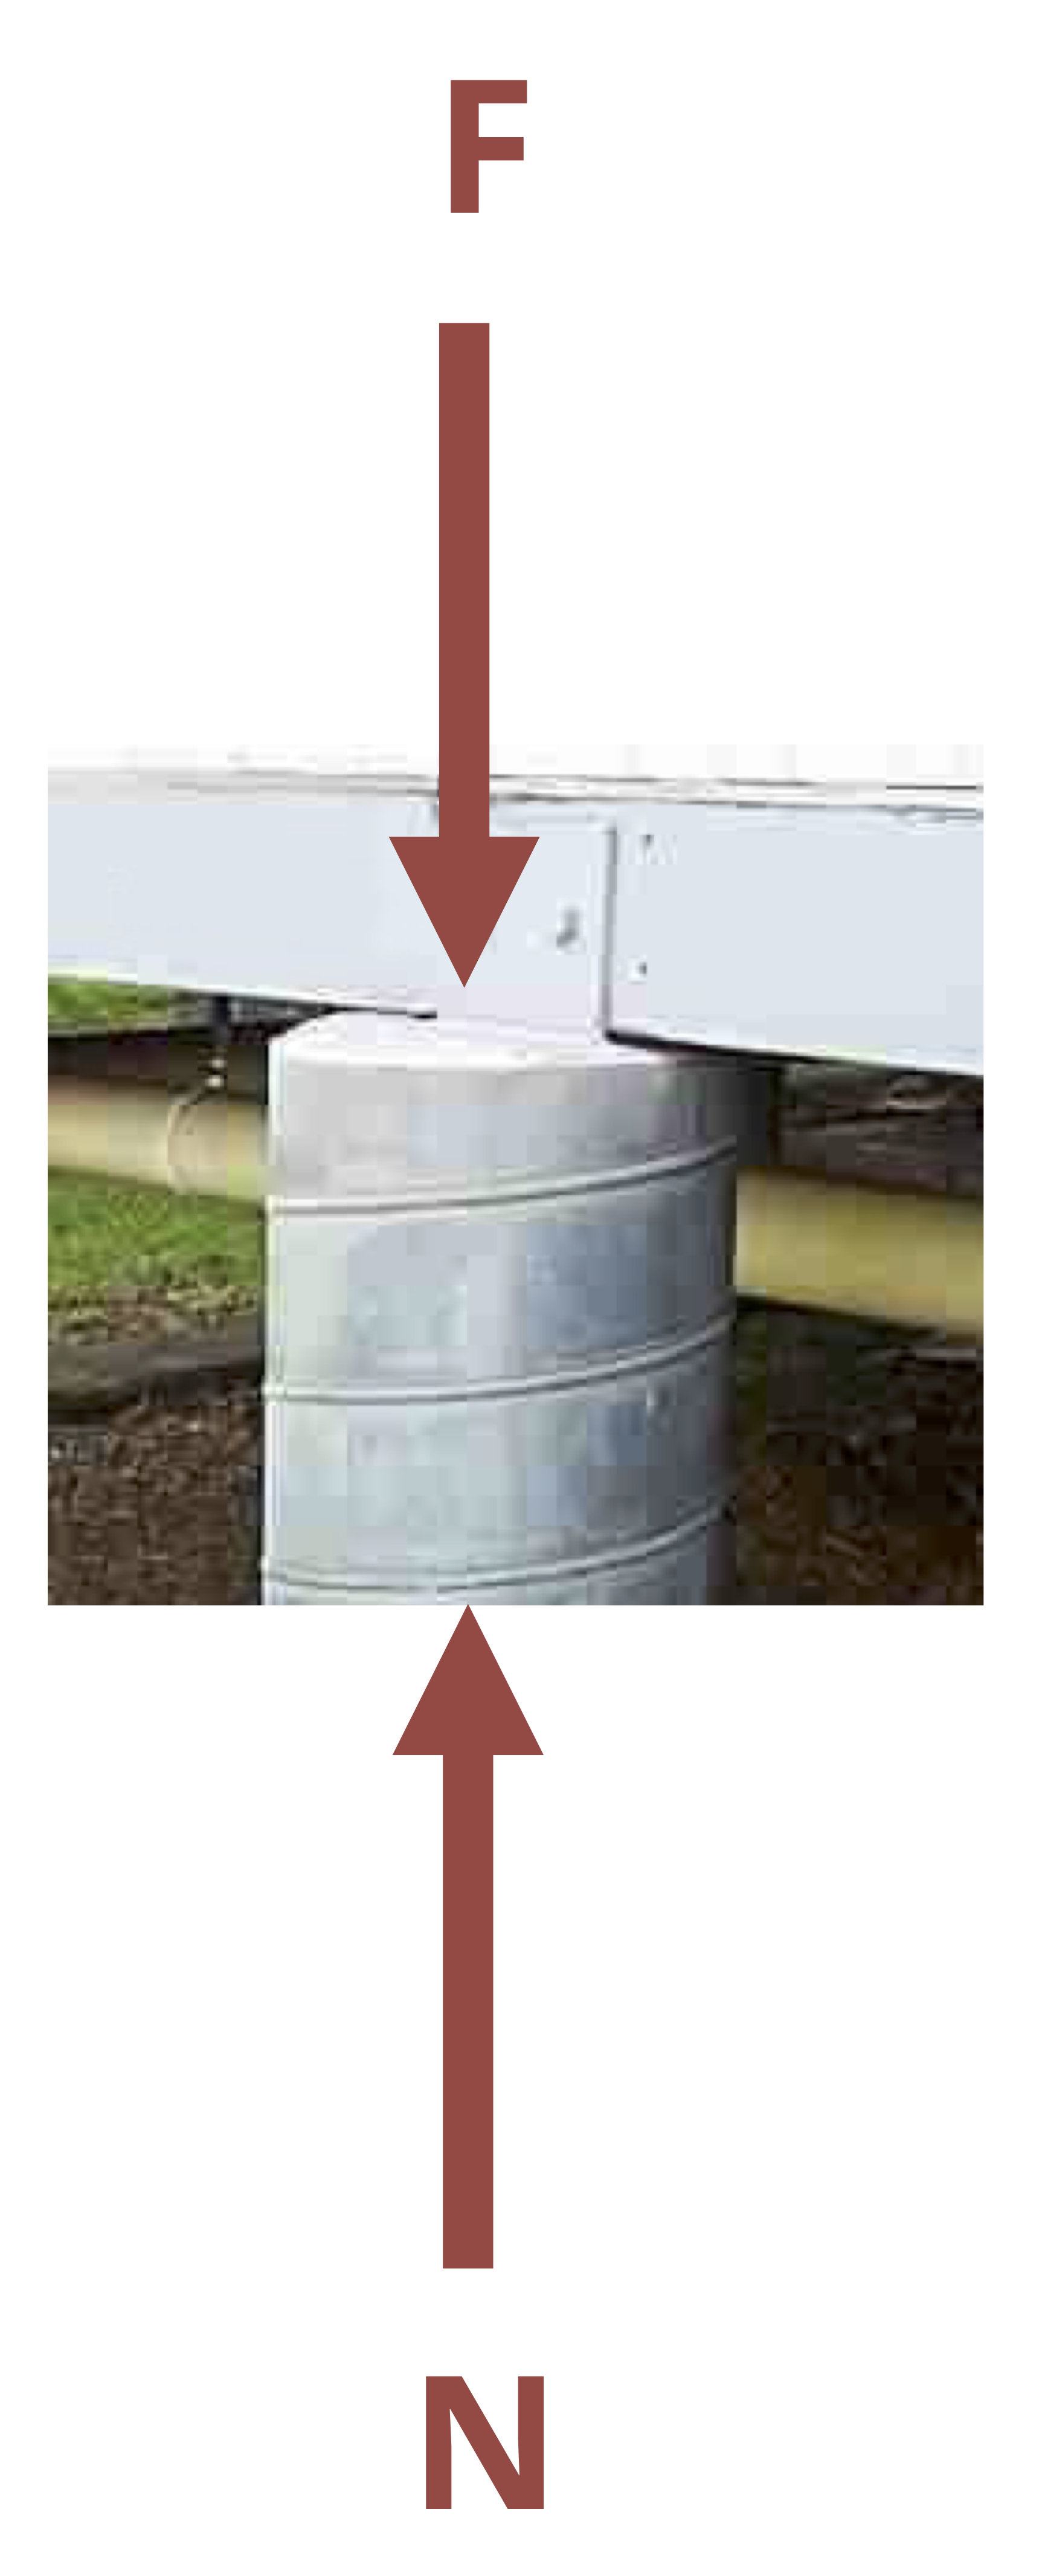
\includegraphics[width=1.41667in,height=\textheight]{images/Updated CH2 examples/example 2.1 part 2.png}
\end{center}

\[
\sum F_y= N-65{~kips}=0
\]

The column has a circular cross-section of area
\(A=\pi(2)^2=4 \pi{~in.}^2\).

The average normal stress can now be found from:

\[
\sigma=\frac{N}{A}=\frac{65{~kips}}{4 \pi{~in.}^2}=5.17{~ksi}
\]

\begin{enumerate}
\def\labelenumi{\arabic{enumi}.}
\setcounter{enumi}{1}
\tightlist
\item
  Use the average normal stress equation again, but this time the stress
  is known to be 4 ksi. The loading has not changed so the internal
  normal force will still be 65 kips.
\end{enumerate}

\[
\sigma=\frac{N}{A} \rightarrow A=\frac{N}{\sigma}=\frac{65{~kips}}{4{~ksi}}=16.25 {~in}^2
\]

Since \(A=\pi r^2\) we can find
\(r=\sqrt{\frac{A}{\pi}}=\sqrt{\frac{16.25{~in.}^2}{\pi}}=2.27{~in}\).

Then \(d=2 r=2 * 2.27{~in.}=4.55{~in.}\)

Note that this is the minimum required diameter to ensure the average
normal stress does not exceed 4 ksi. If the diameter is any smaller than
this, the stress will exceed the 4 ksi limit.

\end{tcolorbox}

\end{example}

\end{tcolorbox}

Sometimes the loading or cross-sectional area of the body will change,
resulting in a change in stress. In these cases the stress can be
calculated separately in each segment of the body by first finding the
internal load in each segment and then dividing the internal load by the
cross-sectional area of the respective segment. Different parts of the
body may experience different stresses. Generally the highest stress is
of most importance as that is the stress that typically determines
whether the body will break. Because we do not know in advance where the
largest stress is, however, it is typically necessary to calculate the
stress at each different cross-section in order to determine the highest
stress. See Example~\ref{exm-2.2} for a demonstration.

\begin{tcolorbox}[enhanced jigsaw, colback=white, colframe=quarto-callout-tip-color-frame, toptitle=1mm, arc=.35mm, bottomrule=.15mm, toprule=.15mm, opacitybacktitle=0.6, title={Example 2.2}, coltitle=black, breakable, colbacktitle=quarto-callout-tip-color!10!white, bottomtitle=1mm, titlerule=0mm, opacityback=0, leftrule=.75mm, left=2mm, rightrule=.15mm]

\begin{example}[]\protect\hypertarget{exm-2.2}{}\label{exm-2.2}

~

Two hollow pipes are welded together as shown. Pipe (1) has an outer
diameter of 70 mm and an inner diameter of 40 mm while pipe (2) has an
outer diameter of 110 mm and an inner diameter of 60 mm. Forces are
applied at the end of each pipe and at the weld, where
F\textsubscript{1} = 40 kN, F\textsubscript{2} = 70 kN, and
F\textsubscript{3} = 30 kN. Determine the average normal stress in each
pipe.

\begin{center}
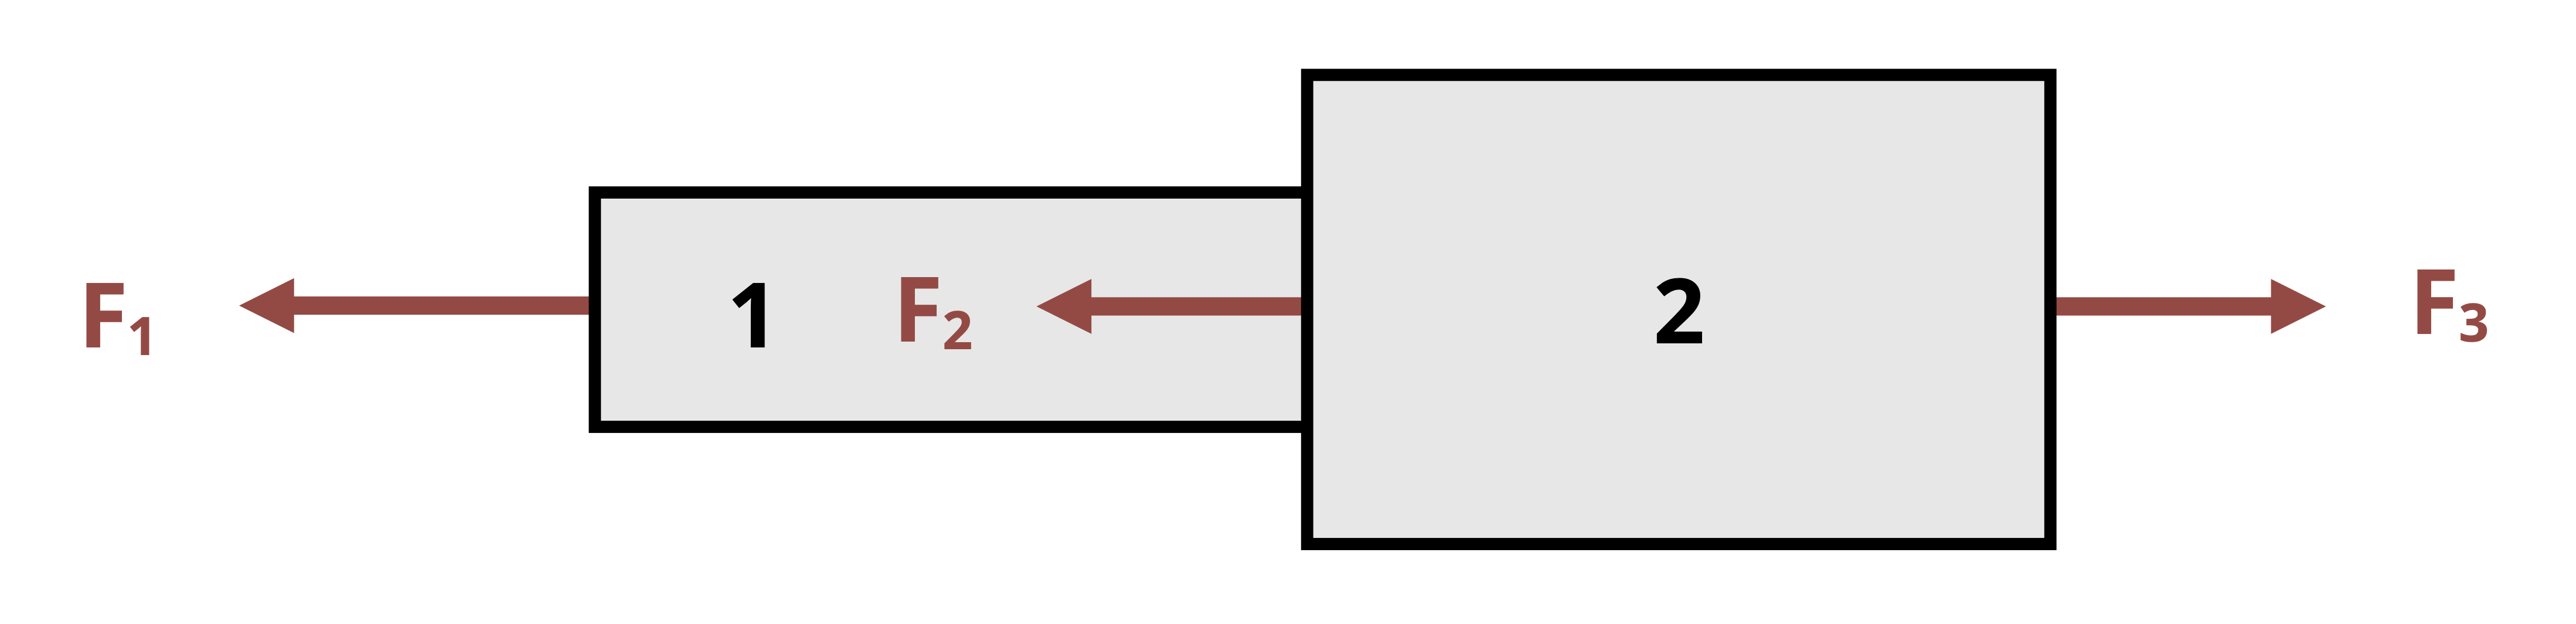
\includegraphics[width=3.40625in,height=\textheight]{images/Updated CH2 examples/example 2.2 part 1.png}
\end{center}

\begin{tcolorbox}[enhanced jigsaw, colback=white, colframe=quarto-callout-tip-color-frame, toptitle=1mm, arc=.35mm, bottomrule=.15mm, toprule=.15mm, opacitybacktitle=0.6, title={Solution}, coltitle=black, breakable, colbacktitle=quarto-callout-tip-color!10!white, bottomtitle=1mm, titlerule=0mm, opacityback=0, leftrule=.75mm, left=2mm, rightrule=.15mm]

We can calculate average normal stress using \(\sigma=\frac{N}{A}\) so
we will need to find the area of each pipe and the normal force in each
pipe. This can be done in any order. Starting with the areas:

\[
\begin{aligned}
& A_1=\pi\left(0.035^2-0.02^2\right)=0.00259{~m}^2 \\
& A_2=\pi\left(0.055^2-0.03^2\right)=0.00668{~m}^2
\end{aligned}
\]

The internal loads can be found by cutting a cross-section through each
pipe, drawing a free body diagram, and writing an equilibrium equation.

\begin{center}
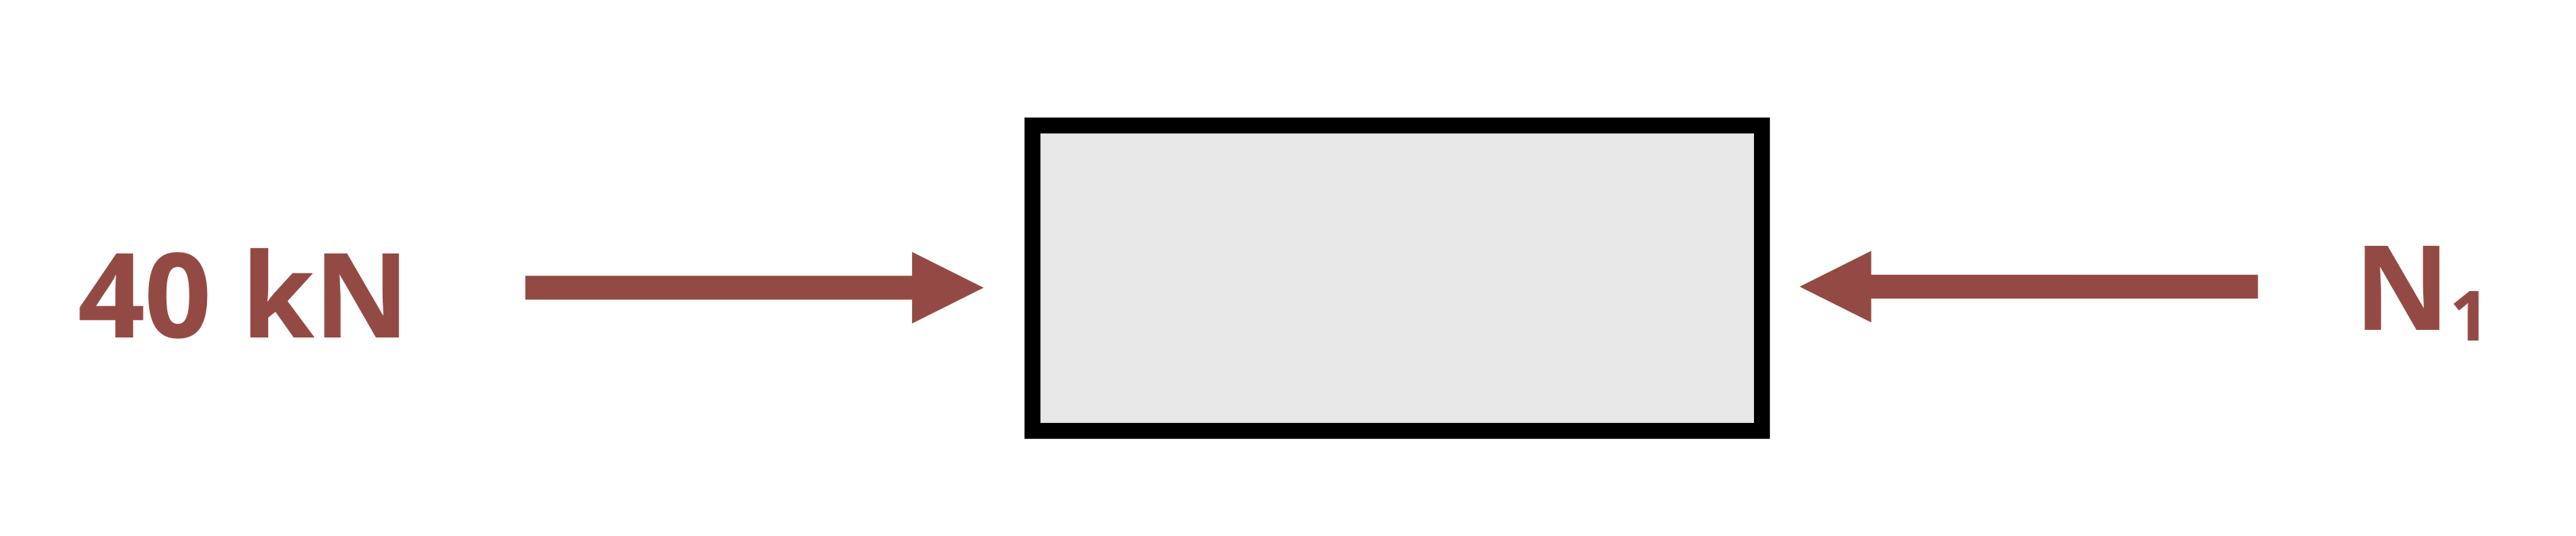
\includegraphics[width=2.8125in,height=\textheight]{images/Updated CH2 examples/example 2.2 part 2.png}
\end{center}

\begin{center}
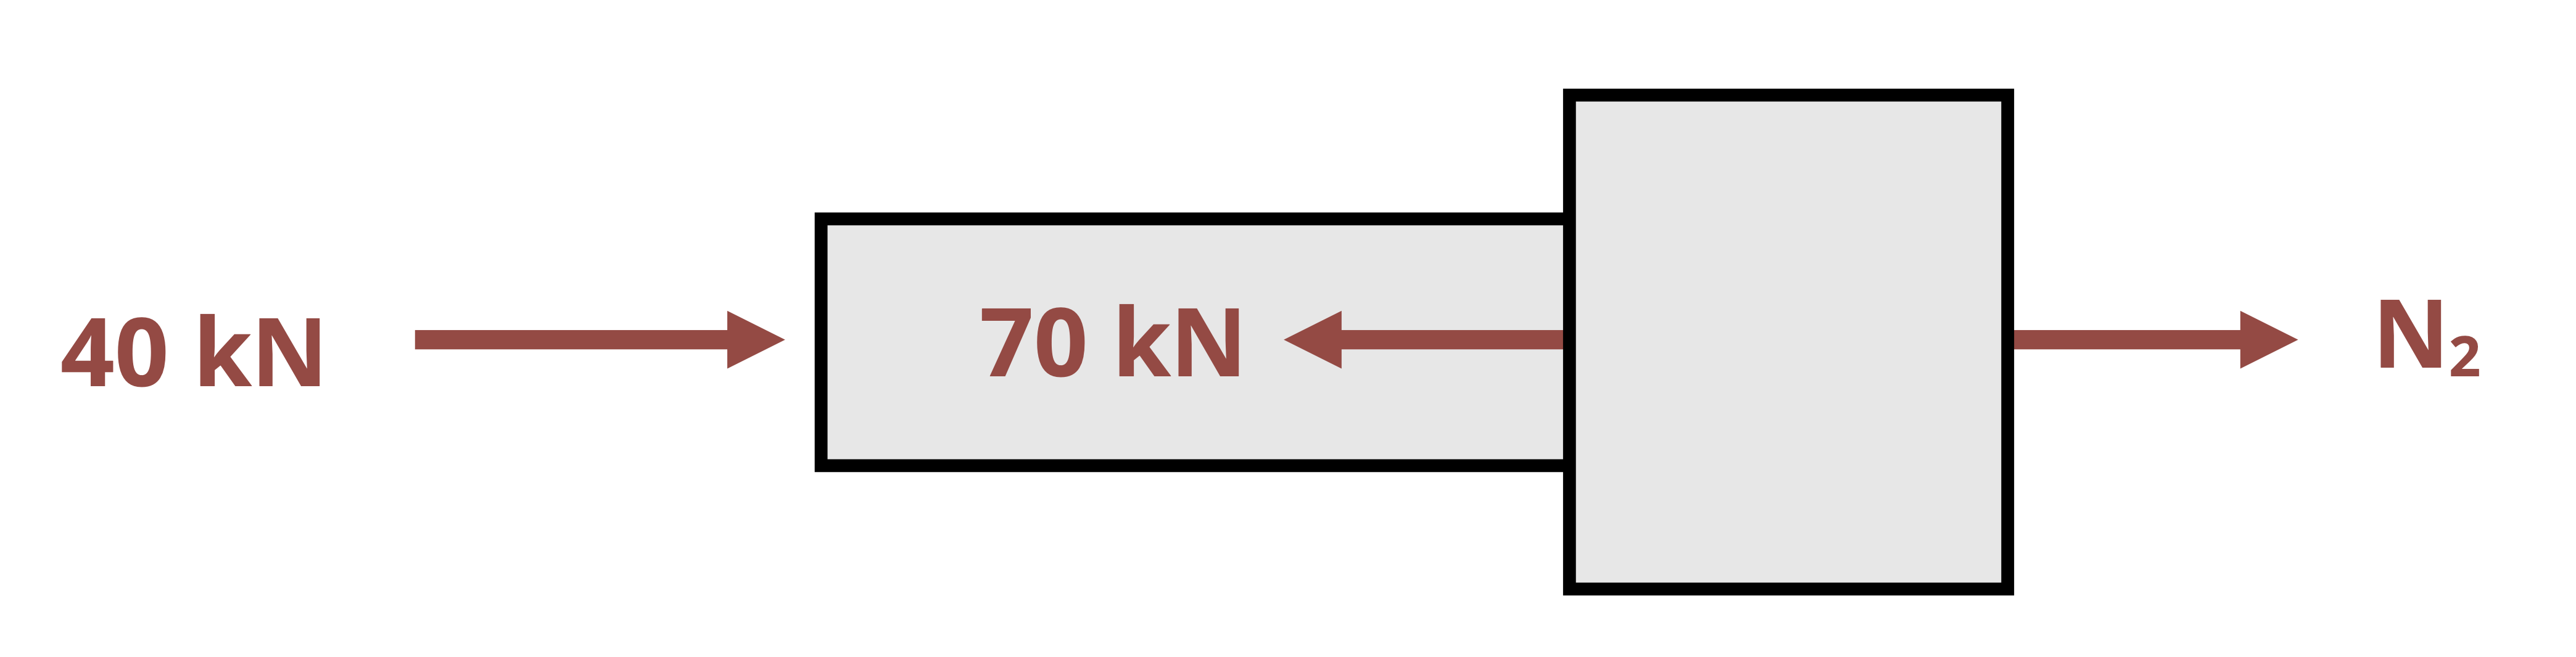
\includegraphics[width=2.71875in,height=\textheight]{images/Updated CH2 examples/example 2.2 part 3.png}
\end{center}

\[
\begin{aligned}
&\sum F_x=40{~kN}-N_1=0 \quad \rightarrow \quad N_1=40{~kN} \\
&\sum F_x=40{~kN}-70{~kN}+N_2=0 \quad \rightarrow \quad N_2=30{~kN}
\end{aligned}
\]

Note that we may choose to draw the internal load in either tension or
compression. The answer must be compared to the free body diagram. A
positive answer from the equilibrium equation indicates that the
direction drawn on the free body diagram was correct. Although both
answers here were positive, it can be seen in the free body diagrams
that N\textsubscript{1} was drawn in compression and N\textsubscript{2}
was drawn in tension. These positive answers indicate that the drawings
are correct. N\textsubscript{1} is 40 kN in compression and
N\textsubscript{2} is 30 kN in tension.

Note also that it is acceptable to draw a free body diagram of either
side of the cross-section. This will not change the result. Perhaps it
would have been easier to draw the right-hand-side of section 2.

\begin{center}
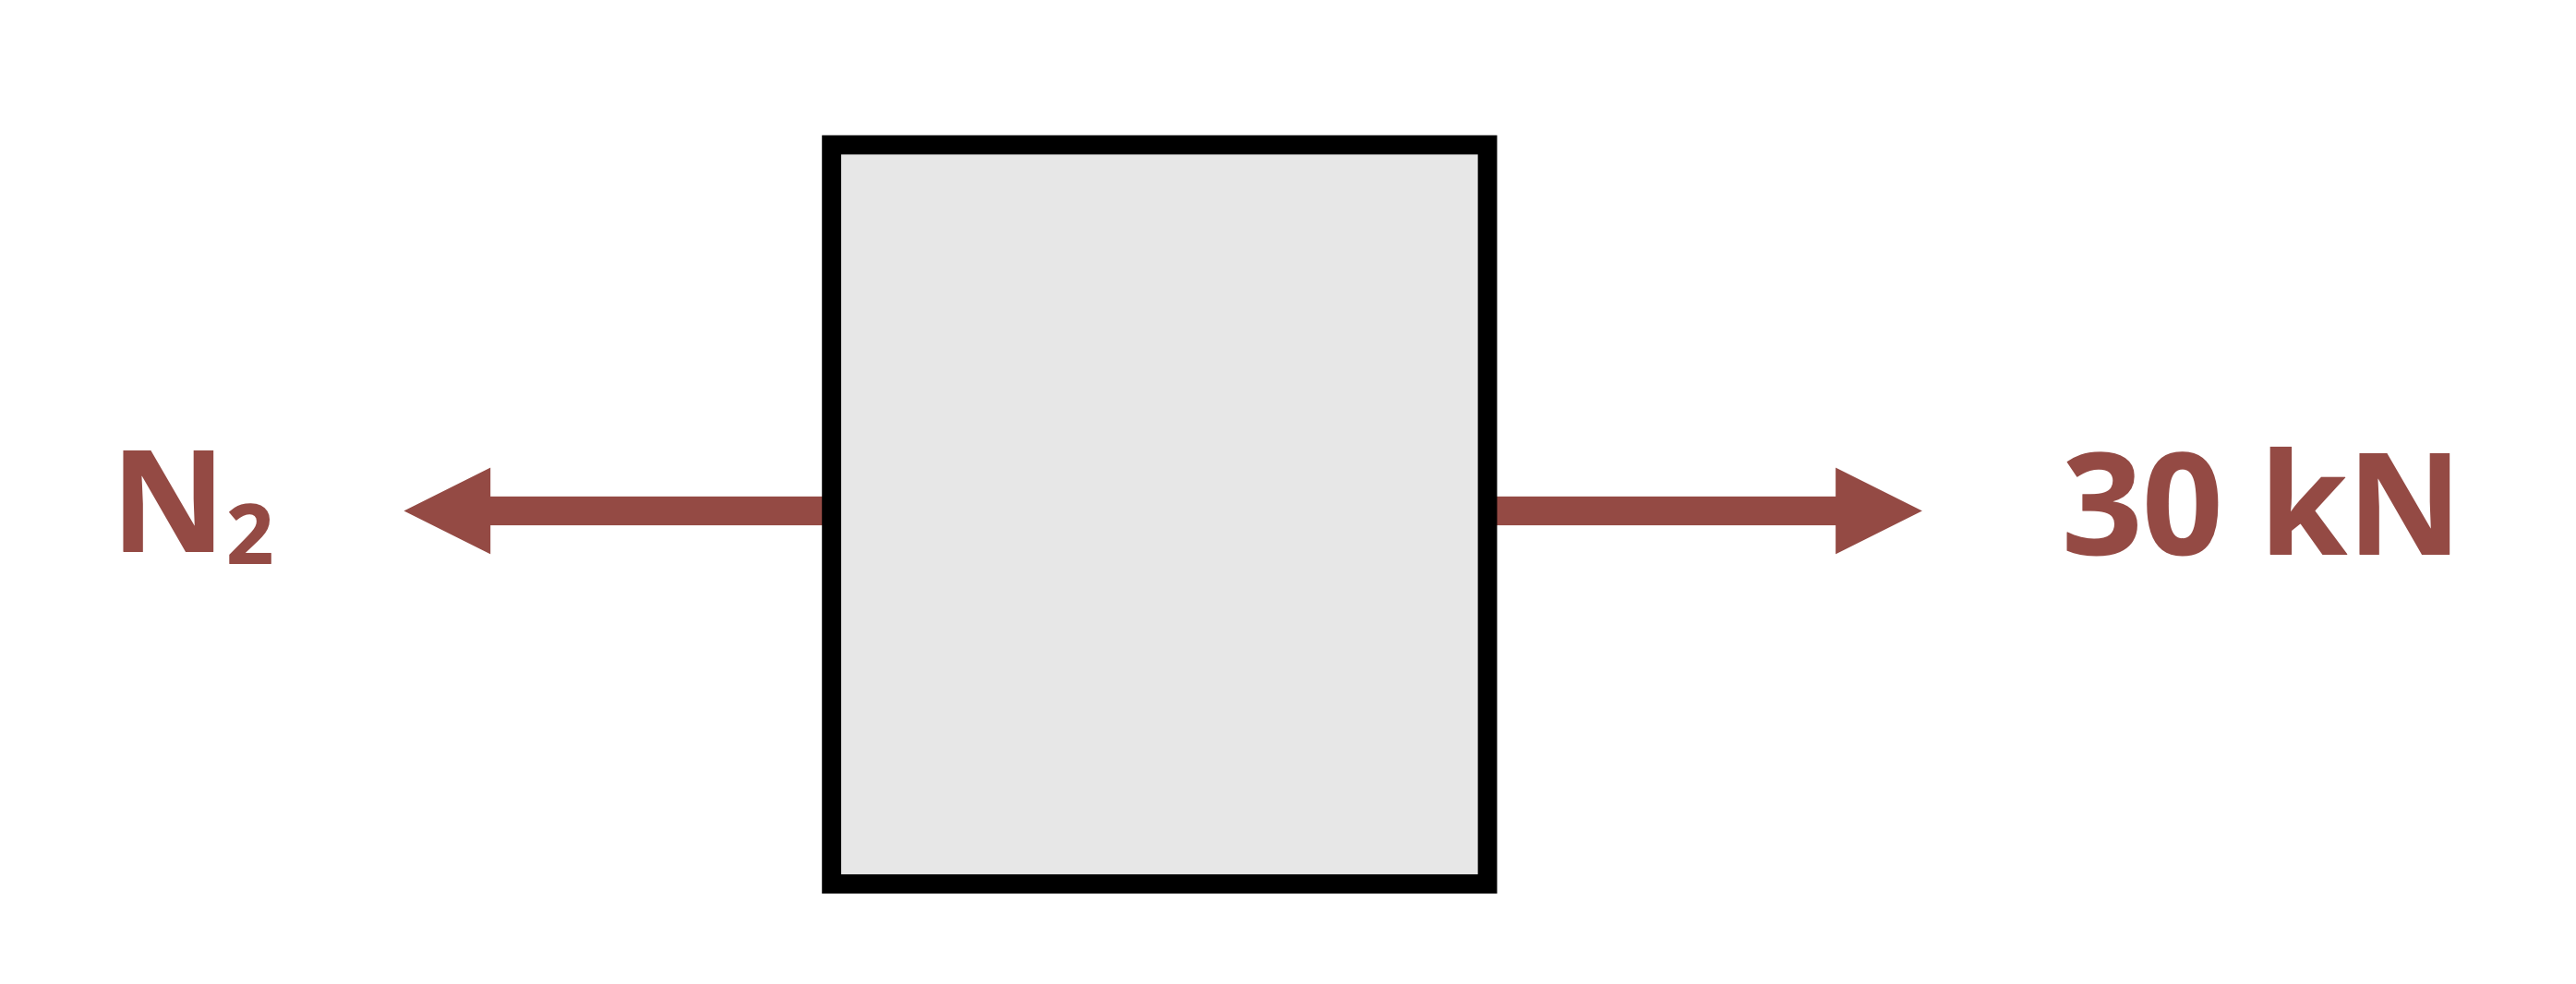
\includegraphics[width=2.45833in,height=\textheight]{images/Updated CH2 examples/example 2.2 part 4.png}
\end{center}

\[
\sum F_x=30{~kN}+N_2=0 \quad \rightarrow \quad N_2=30{~kN}
\]

We again find that N\textsubscript{2} is 30 kN in tension. You may
always choose to draw either side of a cross-section. Make sure to
include everything to that side of your cut, all the way to the end of
the structure (e.g.~do not stop at the weld).

Now that the areas and internal loads are known we can calculate the
internal normal stresses.

\[
\begin{gathered}
\sigma_1=\frac{N_1}{A_1}=\frac{-40,000{~N}}{0.00259{~m}^2}=-15.4{~MPa} \\
\sigma_2=\frac{N_2}{A_2}=\frac{30,000{~N}}{0.00668{~m}^2}=4.49{~MPa}
\end{gathered}
\]

\end{tcolorbox}

\end{example}

\end{tcolorbox}

\begin{tcolorbox}[enhanced jigsaw, colback=white, colframe=quarto-callout-warning-color-frame, toptitle=1mm, arc=.35mm, bottomrule=.15mm, toprule=.15mm, opacitybacktitle=0.6, title={Step-by-step: Average Normal Stress}, coltitle=black, breakable, colbacktitle=quarto-callout-warning-color!10!white, bottomtitle=1mm, titlerule=0mm, opacityback=0, leftrule=.75mm, left=2mm, rightrule=.15mm]

\begin{enumerate}
\def\labelenumi{\arabic{enumi}.}
\item
  Use equilibrium equations to determine reaction loads at any supports.
\item
  Cut a cross-section through the member at the point where you want to
  determine the internal normal stress, and draw a free body diagram of
  the member on either side of the cut. Be sure to include everything on
  the chosen side, including external loads, support reactions, and the
  internal normal force.
\item
  Use equilibrium equations to determine the internal normal force (N)
  in the member.
\item
  Determine average normal stress using \(\sigma=\frac{N}{A}\).
\end{enumerate}

\end{tcolorbox}

\section{Average Shear Stress}\label{sec-2.2}

Click to expand

Average shear stress is defined as the internal shear force divided by
the cross-sectional area of the body. While normal forces (and therefore
normal stresses) occur when a body is under tension or compression,
shear forces (and therefore shear stresses) occur when a force is
tangentially applied parallel to the cross-section, resulting in a
sliding motion (Figure~\ref{fig-2.3}).

\begin{figure}

\centering{

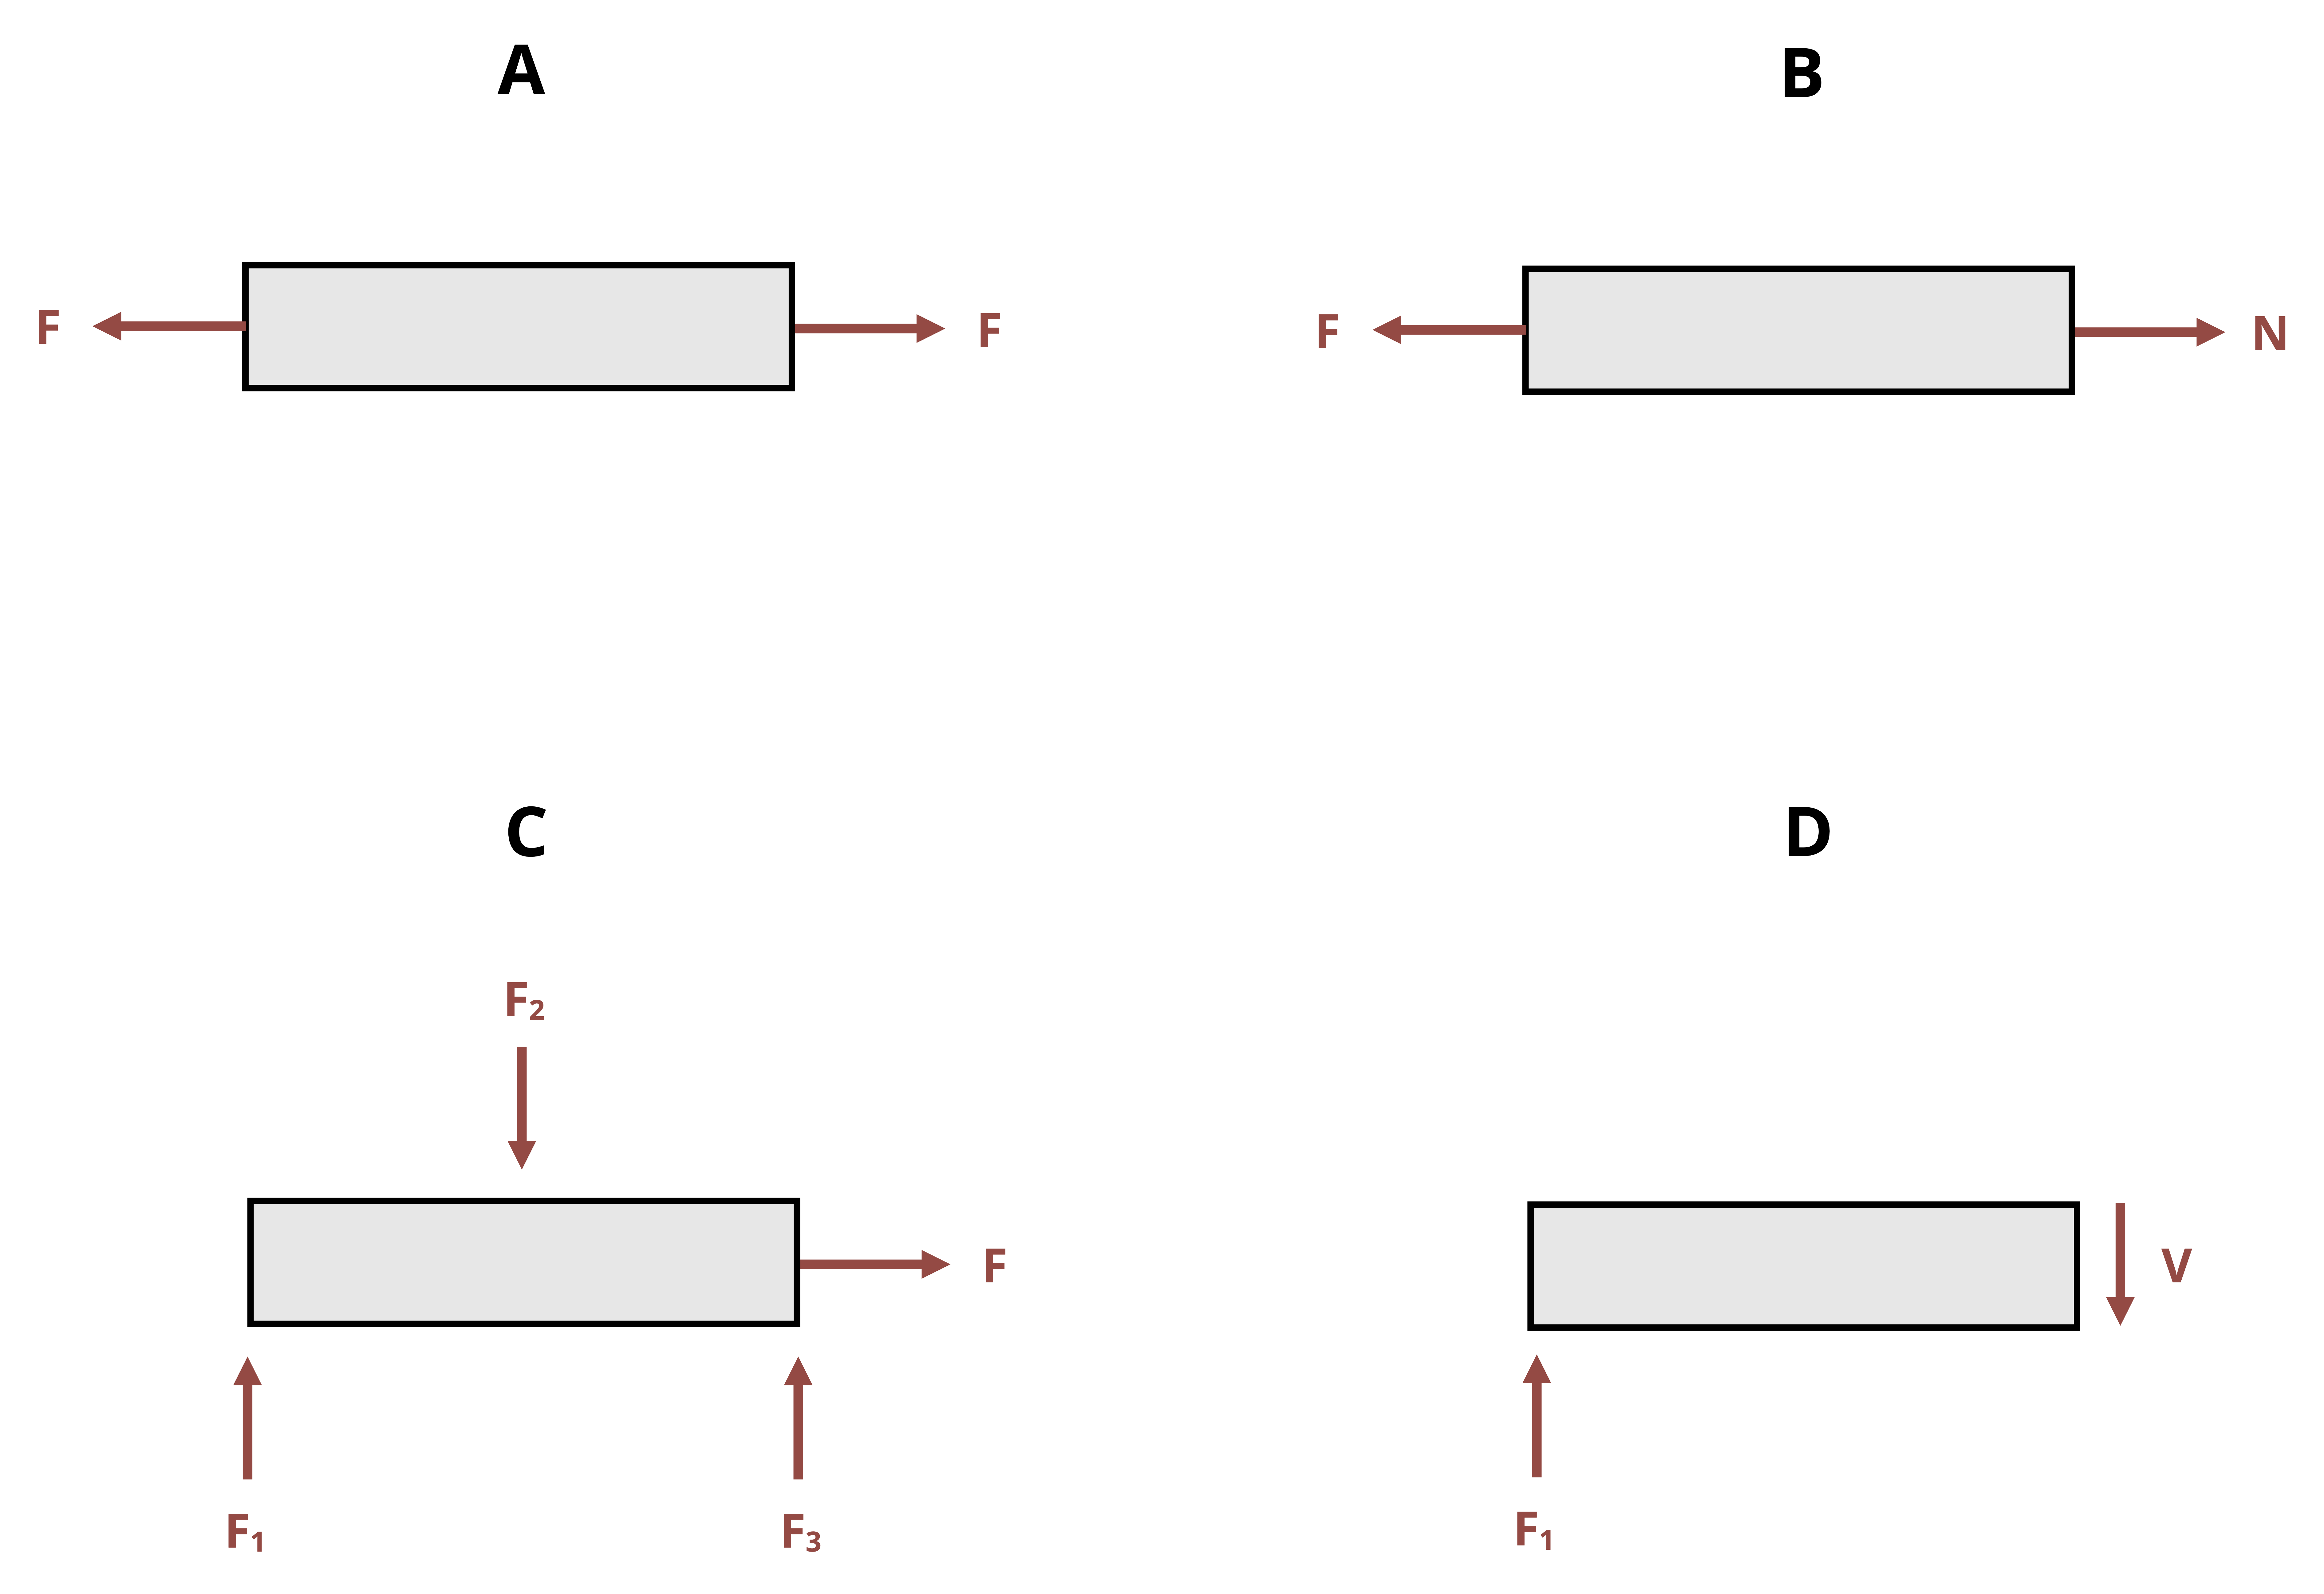
\includegraphics{images/CH2 figures/2.3.png}

}

\caption{\label{fig-2.3}(a) External loads F creating (b) an internal
normal force (N) perpendicular to the cross-section. (c) External loads
F\textsubscript{1}, F\textsubscript{2}, and F\textsubscript{3} creating
(d) an internal shear force (V) parallel to the cross-section. Note that
for diagram (d) to be in equilibrium there would also need to be an
internal bending moment. That has been omitted here for clarity.}

\end{figure}%

Although the basic definition of average normal stress and average shear
stress is the same (force divided by area) there are some differences.
To quickly differentiate which stress we are talking about, shear stress
is denoted by the Greek letter tau (τ).

\begin{equation}\phantomsection\label{eq-2.2}{
\boxed{\tau=\frac{V}{A}}
}\end{equation}

\emph{where}\\
\emph{τ = Average shear stress {[}Pa, psi{]}}\\
\emph{V = Internal shear force {[}N, lb{]}}

\emph{A = Cross-sectional area {[}m\textsuperscript{2},
in.\textsuperscript{2}{]}}

Like normal force, internal shear force can be found by cutting a
cross-section through the body, drawing a free body diagram, and
applying equilibrium equations. See Example~\ref{exm-2.3} for a
demonstration.

\begin{tcolorbox}[enhanced jigsaw, colback=white, colframe=quarto-callout-tip-color-frame, toptitle=1mm, arc=.35mm, bottomrule=.15mm, toprule=.15mm, opacitybacktitle=0.6, title={Example 2.3}, coltitle=black, breakable, colbacktitle=quarto-callout-tip-color!10!white, bottomtitle=1mm, titlerule=0mm, opacityback=0, leftrule=.75mm, left=2mm, rightrule=.15mm]

\begin{example}[]\protect\hypertarget{exm-2.3}{}\label{exm-2.3}

~

A bridge spans a gap of L = 150 ft. The roadway may be considered simply
supported and has a rectangular cross-section of base b = 10 in. and
height h = 6 in. It is subjected to a uniform distributed load of w =
200 lb/ft. Determine the magnitude of the average shear stress in the
cross-section at x = 30 ft and x = 80 ft.

\begin{center}
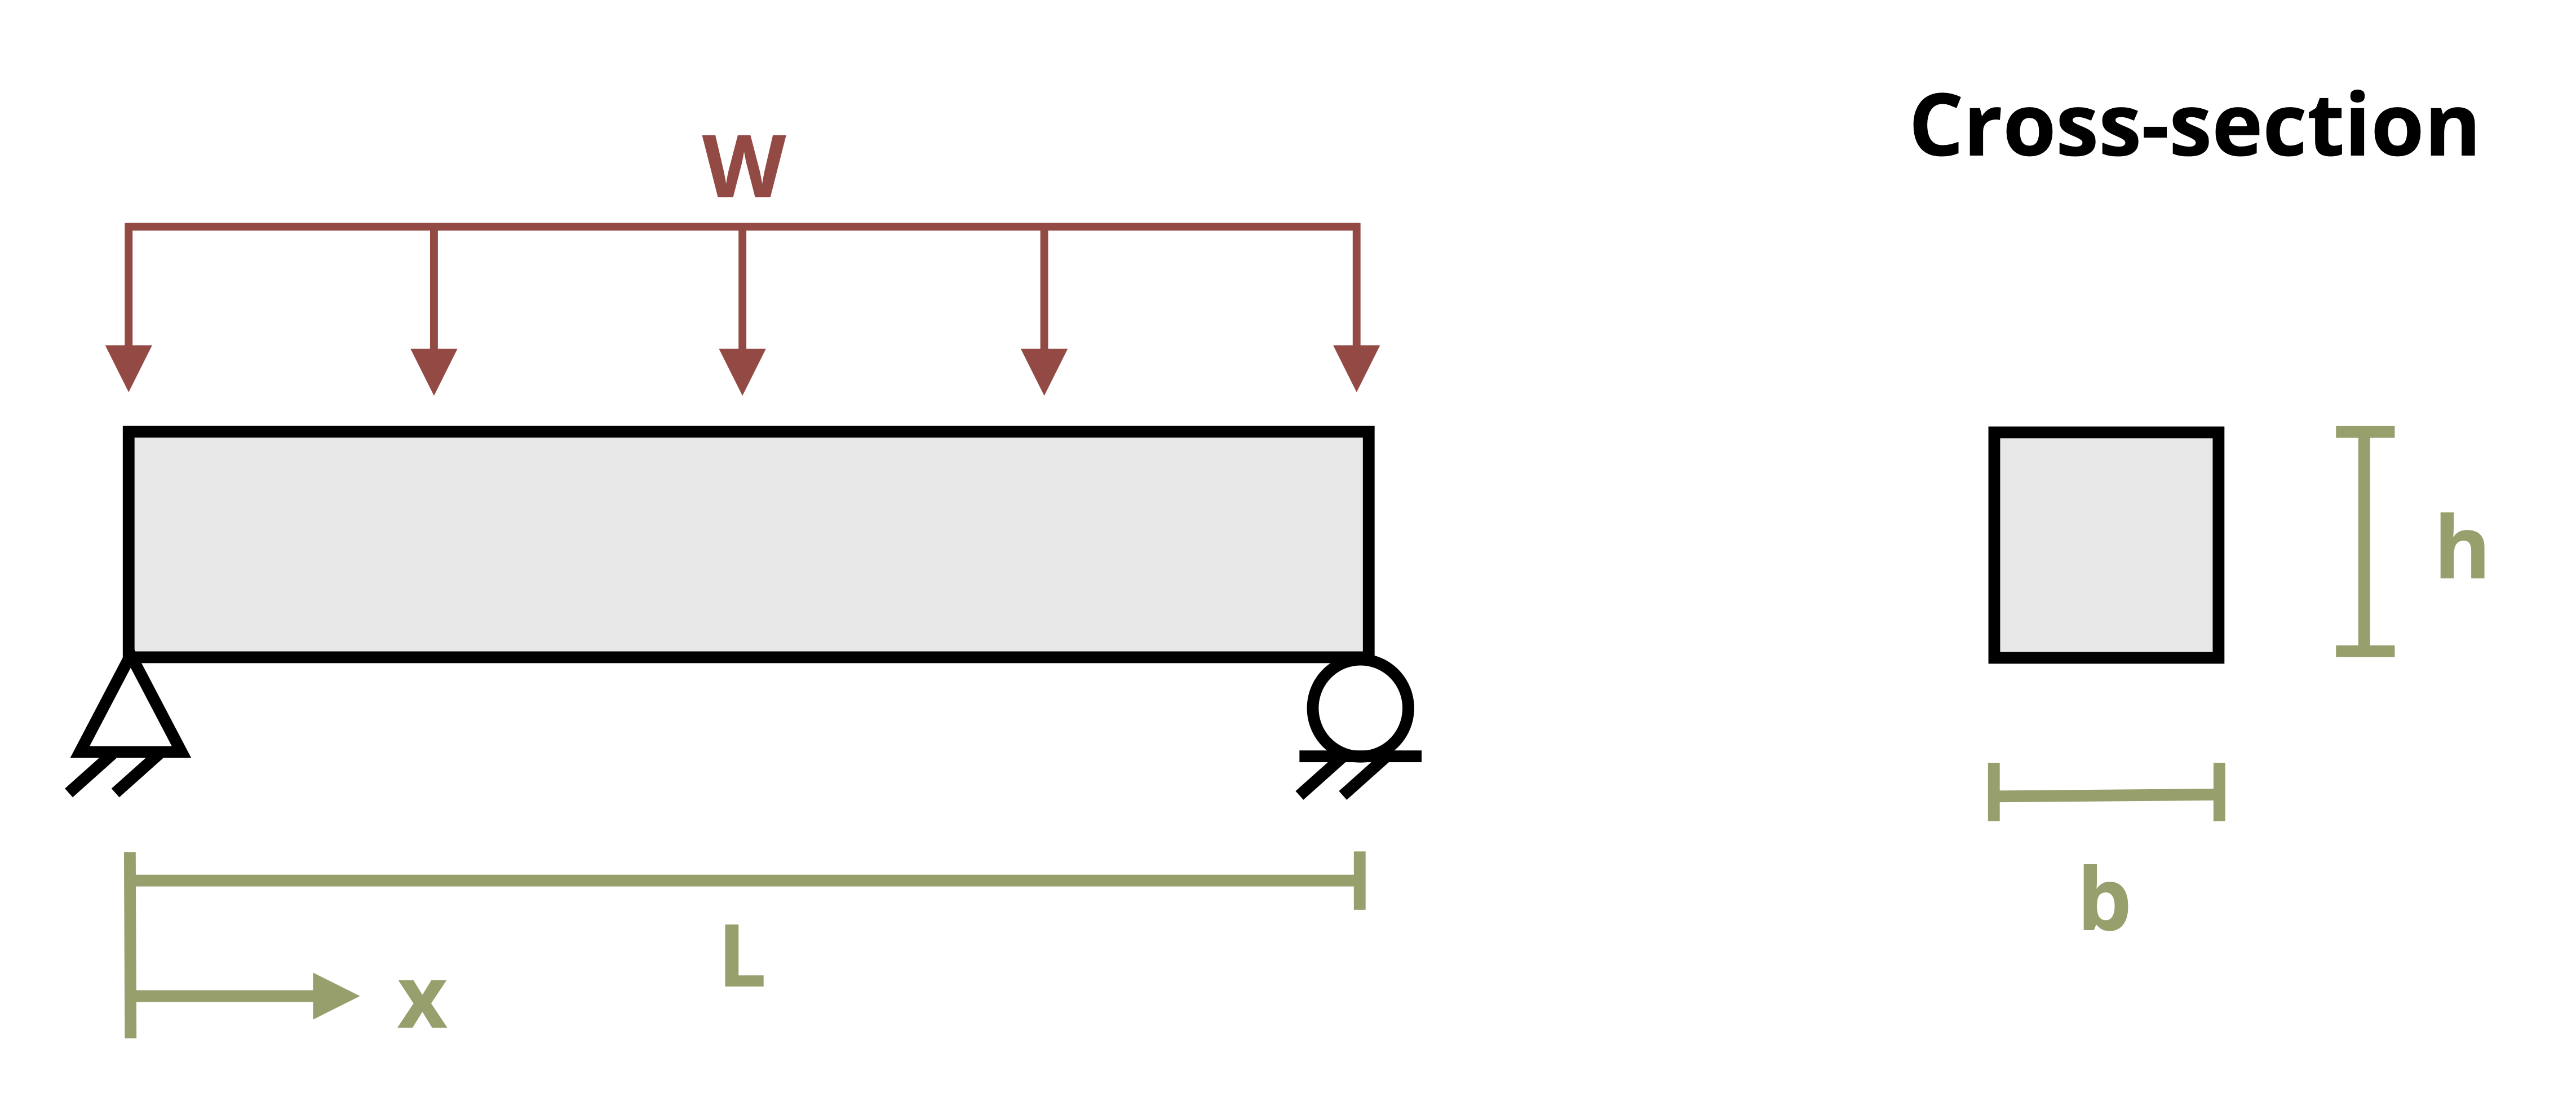
\includegraphics[width=3.46875in,height=\textheight]{images/Updated CH2 examples/example 2.3 part 1.png}
\end{center}

\begin{tcolorbox}[enhanced jigsaw, colback=white, colframe=quarto-callout-tip-color-frame, toptitle=1mm, arc=.35mm, bottomrule=.15mm, toprule=.15mm, opacitybacktitle=0.6, title={Solution}, coltitle=black, breakable, colbacktitle=quarto-callout-tip-color!10!white, bottomtitle=1mm, titlerule=0mm, opacityback=0, leftrule=.75mm, left=2mm, rightrule=.15mm]

Average shear stress can be calculated from \(\tau=\frac{V}{A}\). The
cross-sectional area is \(A=10{~in.}*6{~in.}=60{~in.}^2\)

The reactions at the support can be found by converting the distributed
load into a statically equivalent concentrated load. This load will be
equal to \(F=200{~lb/ft}*150{~ft}=30000{~lb}\) and will be located at
the center of the bridge. Since the loading is symmetric, each support
will support half of this load, or 15000 lb each.

The internal shear force can be found by cutting a cross-section through
the point of interest, drawing a free body diagram, and applying
equilibrium equations. Remember to include the internal loads V and M,
and to again convert the distributed load into a statically equivalent
concentrated load over this portion of the bridge.

At x = 30 ft:

\begin{center}
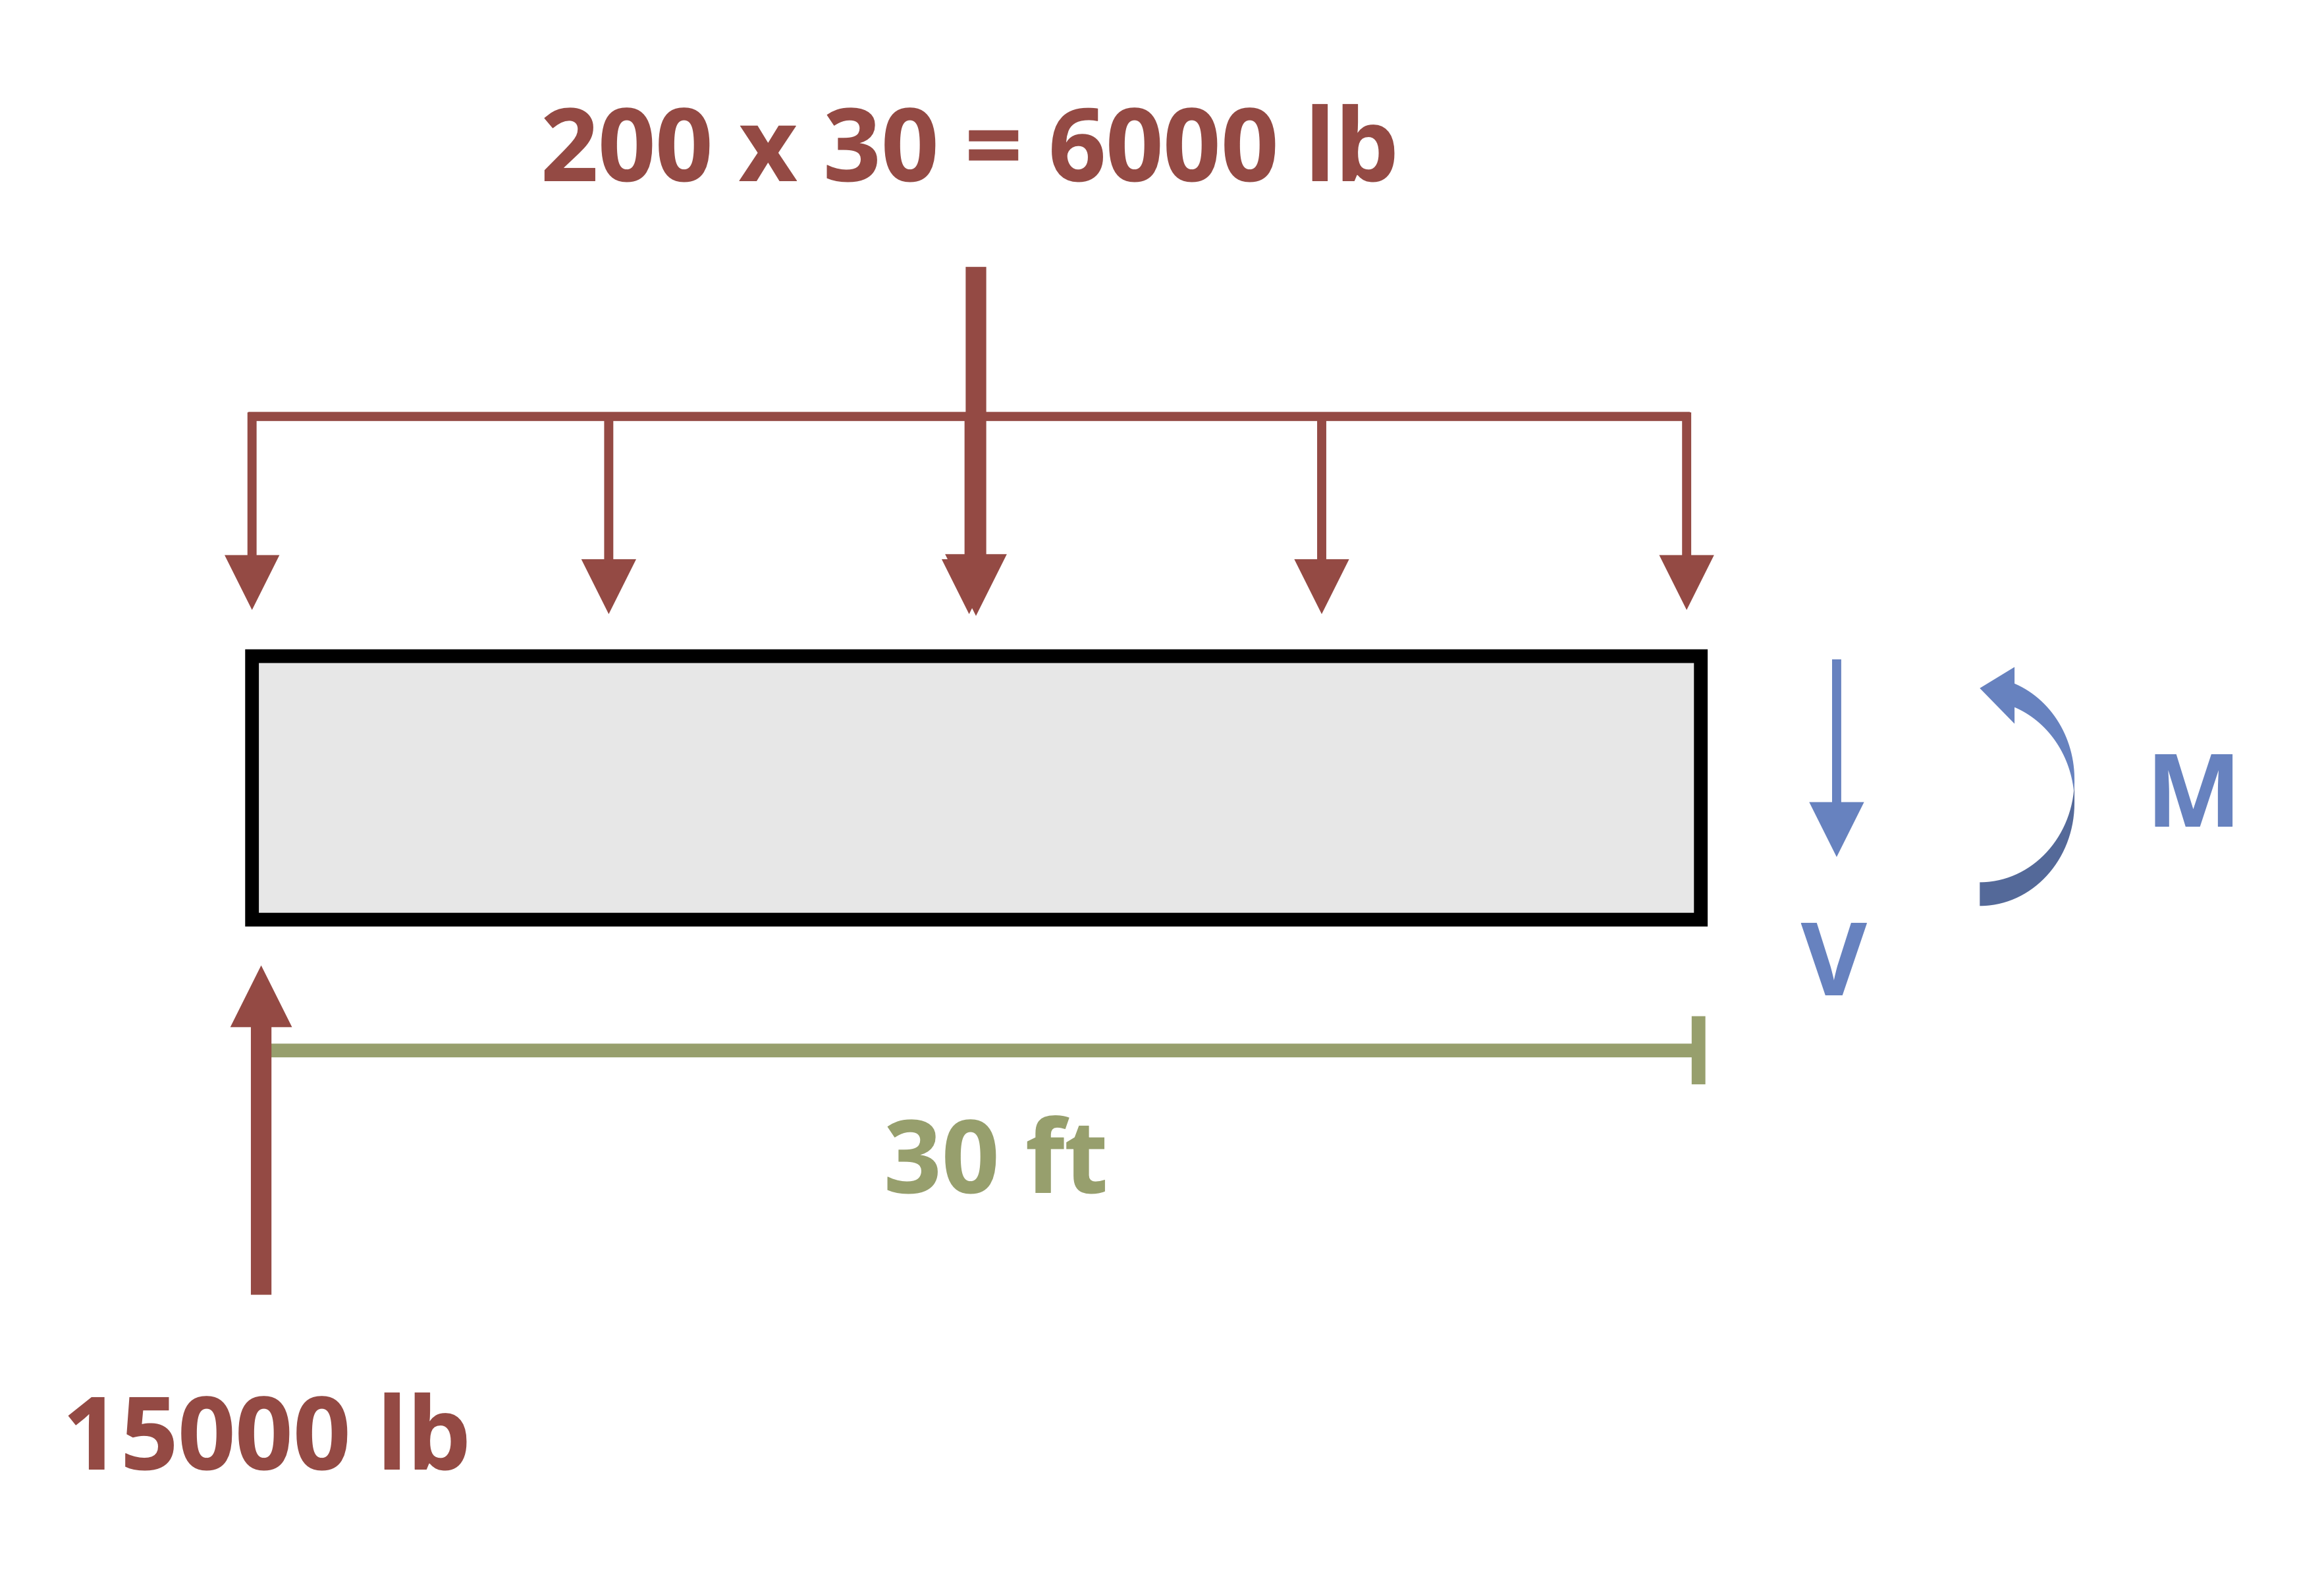
\includegraphics[width=3.41667in,height=\textheight]{images/Updated CH2 examples/example 2.3 part 2.png}
\end{center}

\[
\sum F_y=15,000{~lb}-6,000{~lb}-V=0 \quad \rightarrow \quad V=9,000{~lb}
\]

Note that an internal bending moment is also necessary in order to
maintain equilibrium. We could find M by summing moments about any
point, but it is not needed in order to solve this problem.

The shear stress can now be calculated.

\[
\tau=\frac{V}{A}=\frac{9,000{~lb}}{60{~in.}^2}=150{~psi}
\]

At x = 80 ft:

\begin{center}
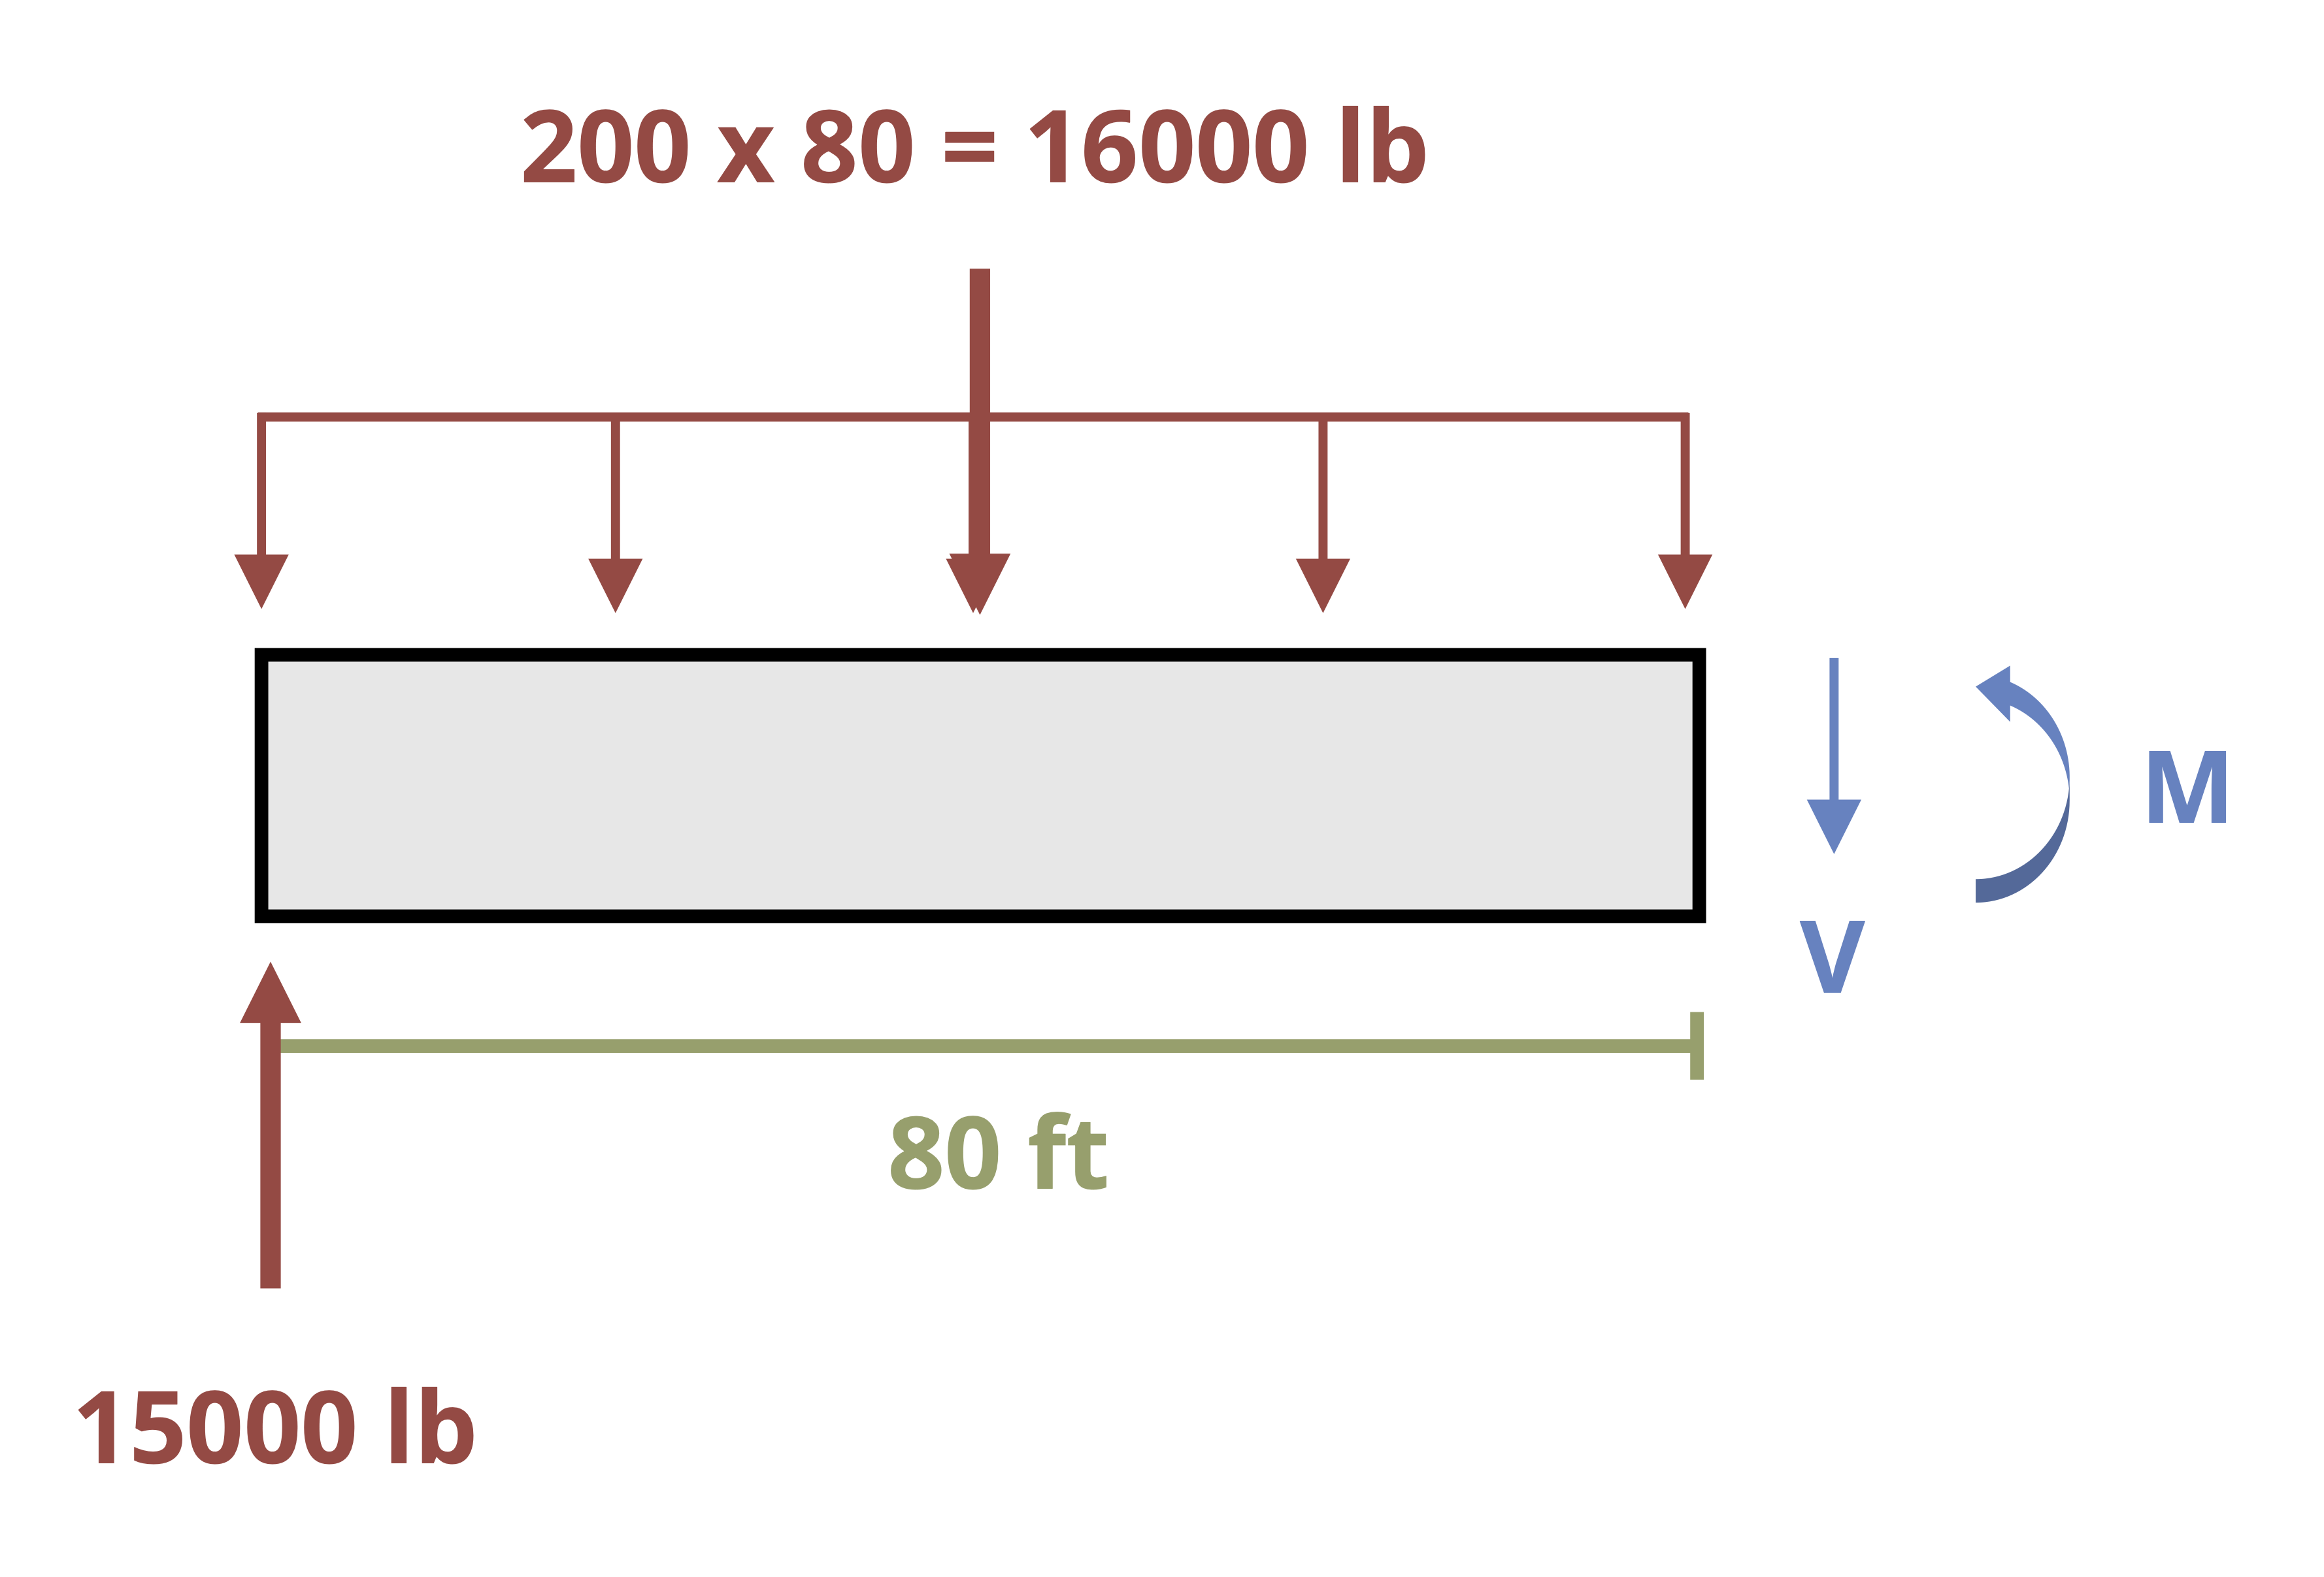
\includegraphics[width=2.96875in,height=\textheight]{images/Updated CH2 examples/example 2.3 part 3.png}
\end{center}

\[
\sum F_y=15,000{~lb}-16,000{~lb}-V=0 \quad \rightarrow \quad V=-1,000{~lb}
\]

Note that the negative sign here simply indicates that V is acting in
the opposite direction of that drawn in the free body diagram. It can be
discarded here as we are calculating the magnitude of the average shear
stress at each point.

\[
\tau=\frac{V}{A}=\frac{1,000{~lb}}{60{~in.}^2}=16.7{~psi}
\]

\end{tcolorbox}

\end{example}

\end{tcolorbox}

Shear stresses are common in both members of a structure and also in the
fasteners between members. Depending on how these connections are formed
we may see multiple shear planes. It is very important to correctly
identify the internal force in the body. Figure~\ref{fig-2.4}
demonstrates the difference between single and double shear
configurations for a pinned joint and the effects on internal shear
force. See Example~\ref{exm-2.4} for an example where double shear
occurs.

\begin{figure}

\centering{

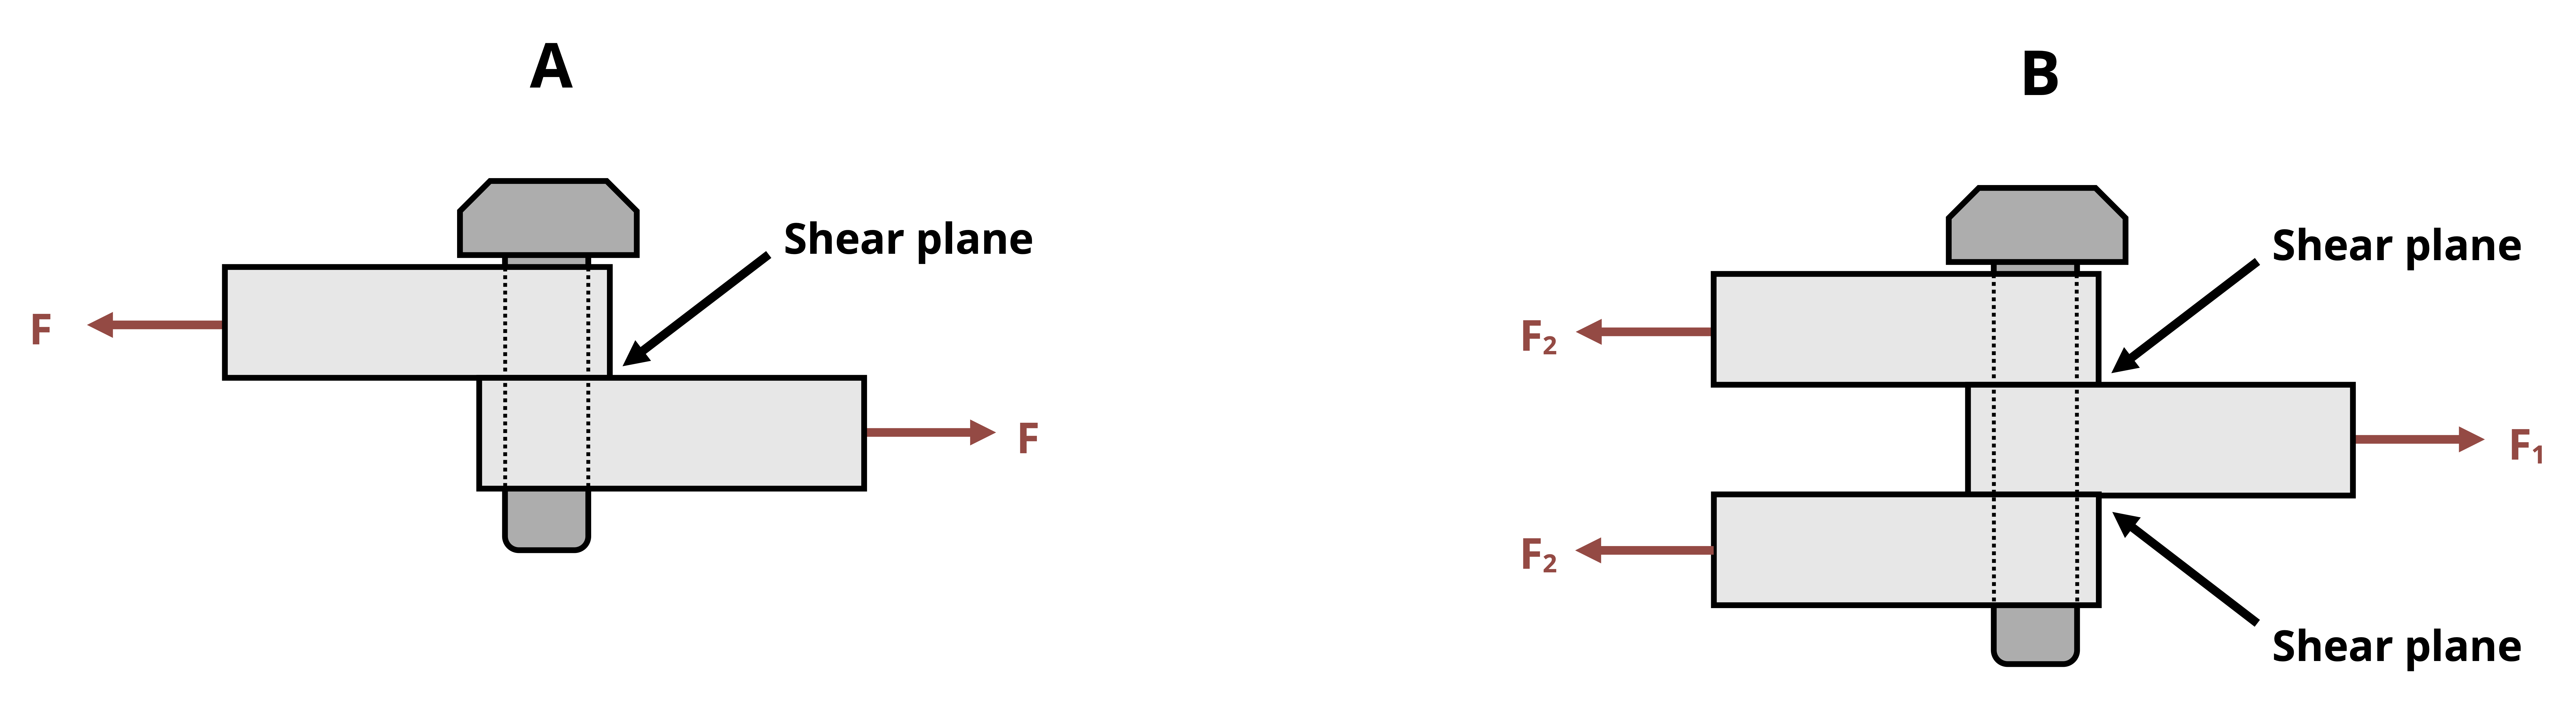
\includegraphics{images/CH2 figures/2.4.png}

}

\caption{\label{fig-2.4}Pins experiencing (a) single shear and (b)
double shear.}

\end{figure}%

\begin{tcolorbox}[enhanced jigsaw, colback=white, colframe=quarto-callout-tip-color-frame, toptitle=1mm, arc=.35mm, bottomrule=.15mm, toprule=.15mm, opacitybacktitle=0.6, title={Example 2.4}, coltitle=black, breakable, colbacktitle=quarto-callout-tip-color!10!white, bottomtitle=1mm, titlerule=0mm, opacityback=0, leftrule=.75mm, left=2mm, rightrule=.15mm]

\begin{example}[]\protect\hypertarget{exm-2.4}{}\label{exm-2.4}

~

A pin made of a tin alloy with an allowable shear stress of 3 ksi is
used to connect a footrest to the frame of a motorcycle. When in motion,
the footrest supports a load of 200 lb which is transferred to the pin.
Determine the required diameter of the pin such that the stress will not
exceed 5 ksi.

\begin{center}
\includegraphics[width=4.48958in,height=\textheight]{images/example 2.4 (new).png}
\end{center}

\begin{tcolorbox}[enhanced jigsaw, colback=white, colframe=quarto-callout-tip-color-frame, toptitle=1mm, arc=.35mm, bottomrule=.15mm, toprule=.15mm, opacitybacktitle=0.6, title={Solution}, coltitle=black, breakable, colbacktitle=quarto-callout-tip-color!10!white, bottomtitle=1mm, titlerule=0mm, opacityback=0, leftrule=.75mm, left=2mm, rightrule=.15mm]

Average shear stress can be calculated from \(\tau=\frac{V}{A}\).
Rearrange this equation to \(A=\frac{V}{\tau}\). Start with a free body
diagram of the pin in order to determine the internal shear force.

From the diagram it should be apparent that the pin is in double shear
and the maximum internal shear force in the pin is 100 lb. Thus the
required cross-sectional area
\(A=\frac{100{~lb}}{3000{~psi}}=0.0333{~in.}^2\).

Since \(A=\frac{\pi}{4} d^2\) the required diameter is
\(d=\sqrt{\frac{0.0333{~in.}^2 * 4}{\pi}}=0.206{~in}\).

\end{tcolorbox}

\end{example}

\end{tcolorbox}

\begin{tcolorbox}[enhanced jigsaw, colback=white, colframe=quarto-callout-warning-color-frame, toptitle=1mm, arc=.35mm, bottomrule=.15mm, toprule=.15mm, opacitybacktitle=0.6, title={Step-by-step: Average Shear stress}, coltitle=black, breakable, colbacktitle=quarto-callout-warning-color!10!white, bottomtitle=1mm, titlerule=0mm, opacityback=0, leftrule=.75mm, left=2mm, rightrule=.15mm]

\begin{enumerate}
\def\labelenumi{\arabic{enumi}.}
\item
  Use equilibrium equations to determine reaction loads at any supports.
\item
  Cut a cross-section through the member at the point where you want to
  determine the internal shear stress, and draw a free body diagram of
  the member on either side of the cut. Be sure to include everything on
  the chosen side, including external loads, support reactions, and the
  internal shear force.
\item
  Use equilibrium equations to determine the internal shear force (V) in
  the member.
\item
  Determine average normal stress using \(\tau=\frac{V}{A}\)
\end{enumerate}

\end{tcolorbox}

\section{Bearing Stress}\label{sec-2.3}

Click to expand

Bearing stress is similar to normal stress, except that it occurs at the
contact area between two bodies instead of within a single body. Bearing
stress is calculated with the average normal stress equation, where the
cross-sectional area is the contact area between the two bodies
(Figure~\ref{fig-2.5}).

\begin{figure}

\centering{

\includegraphics[width=2.82292in,height=\textheight]{images/CH2 figures/2.5.png}

}

\caption{\label{fig-2.5}Circular column sitting upon a rectangular
foundation. Contact areas between a circular and rectangular surface,
and between two rectangular surfaces are shown.}

\end{figure}%

One common situation is contact between two curved edges, such as the
bolt in Figure~\ref{fig-2.6}. In this situation it is common to use the
projected contact area between the curved surfaces, which forms a
rectangle of base d and height t. This greatly simplifies the
calculation, but again represents an average value for the contact or
bearing stress.

\begin{figure}

\centering{

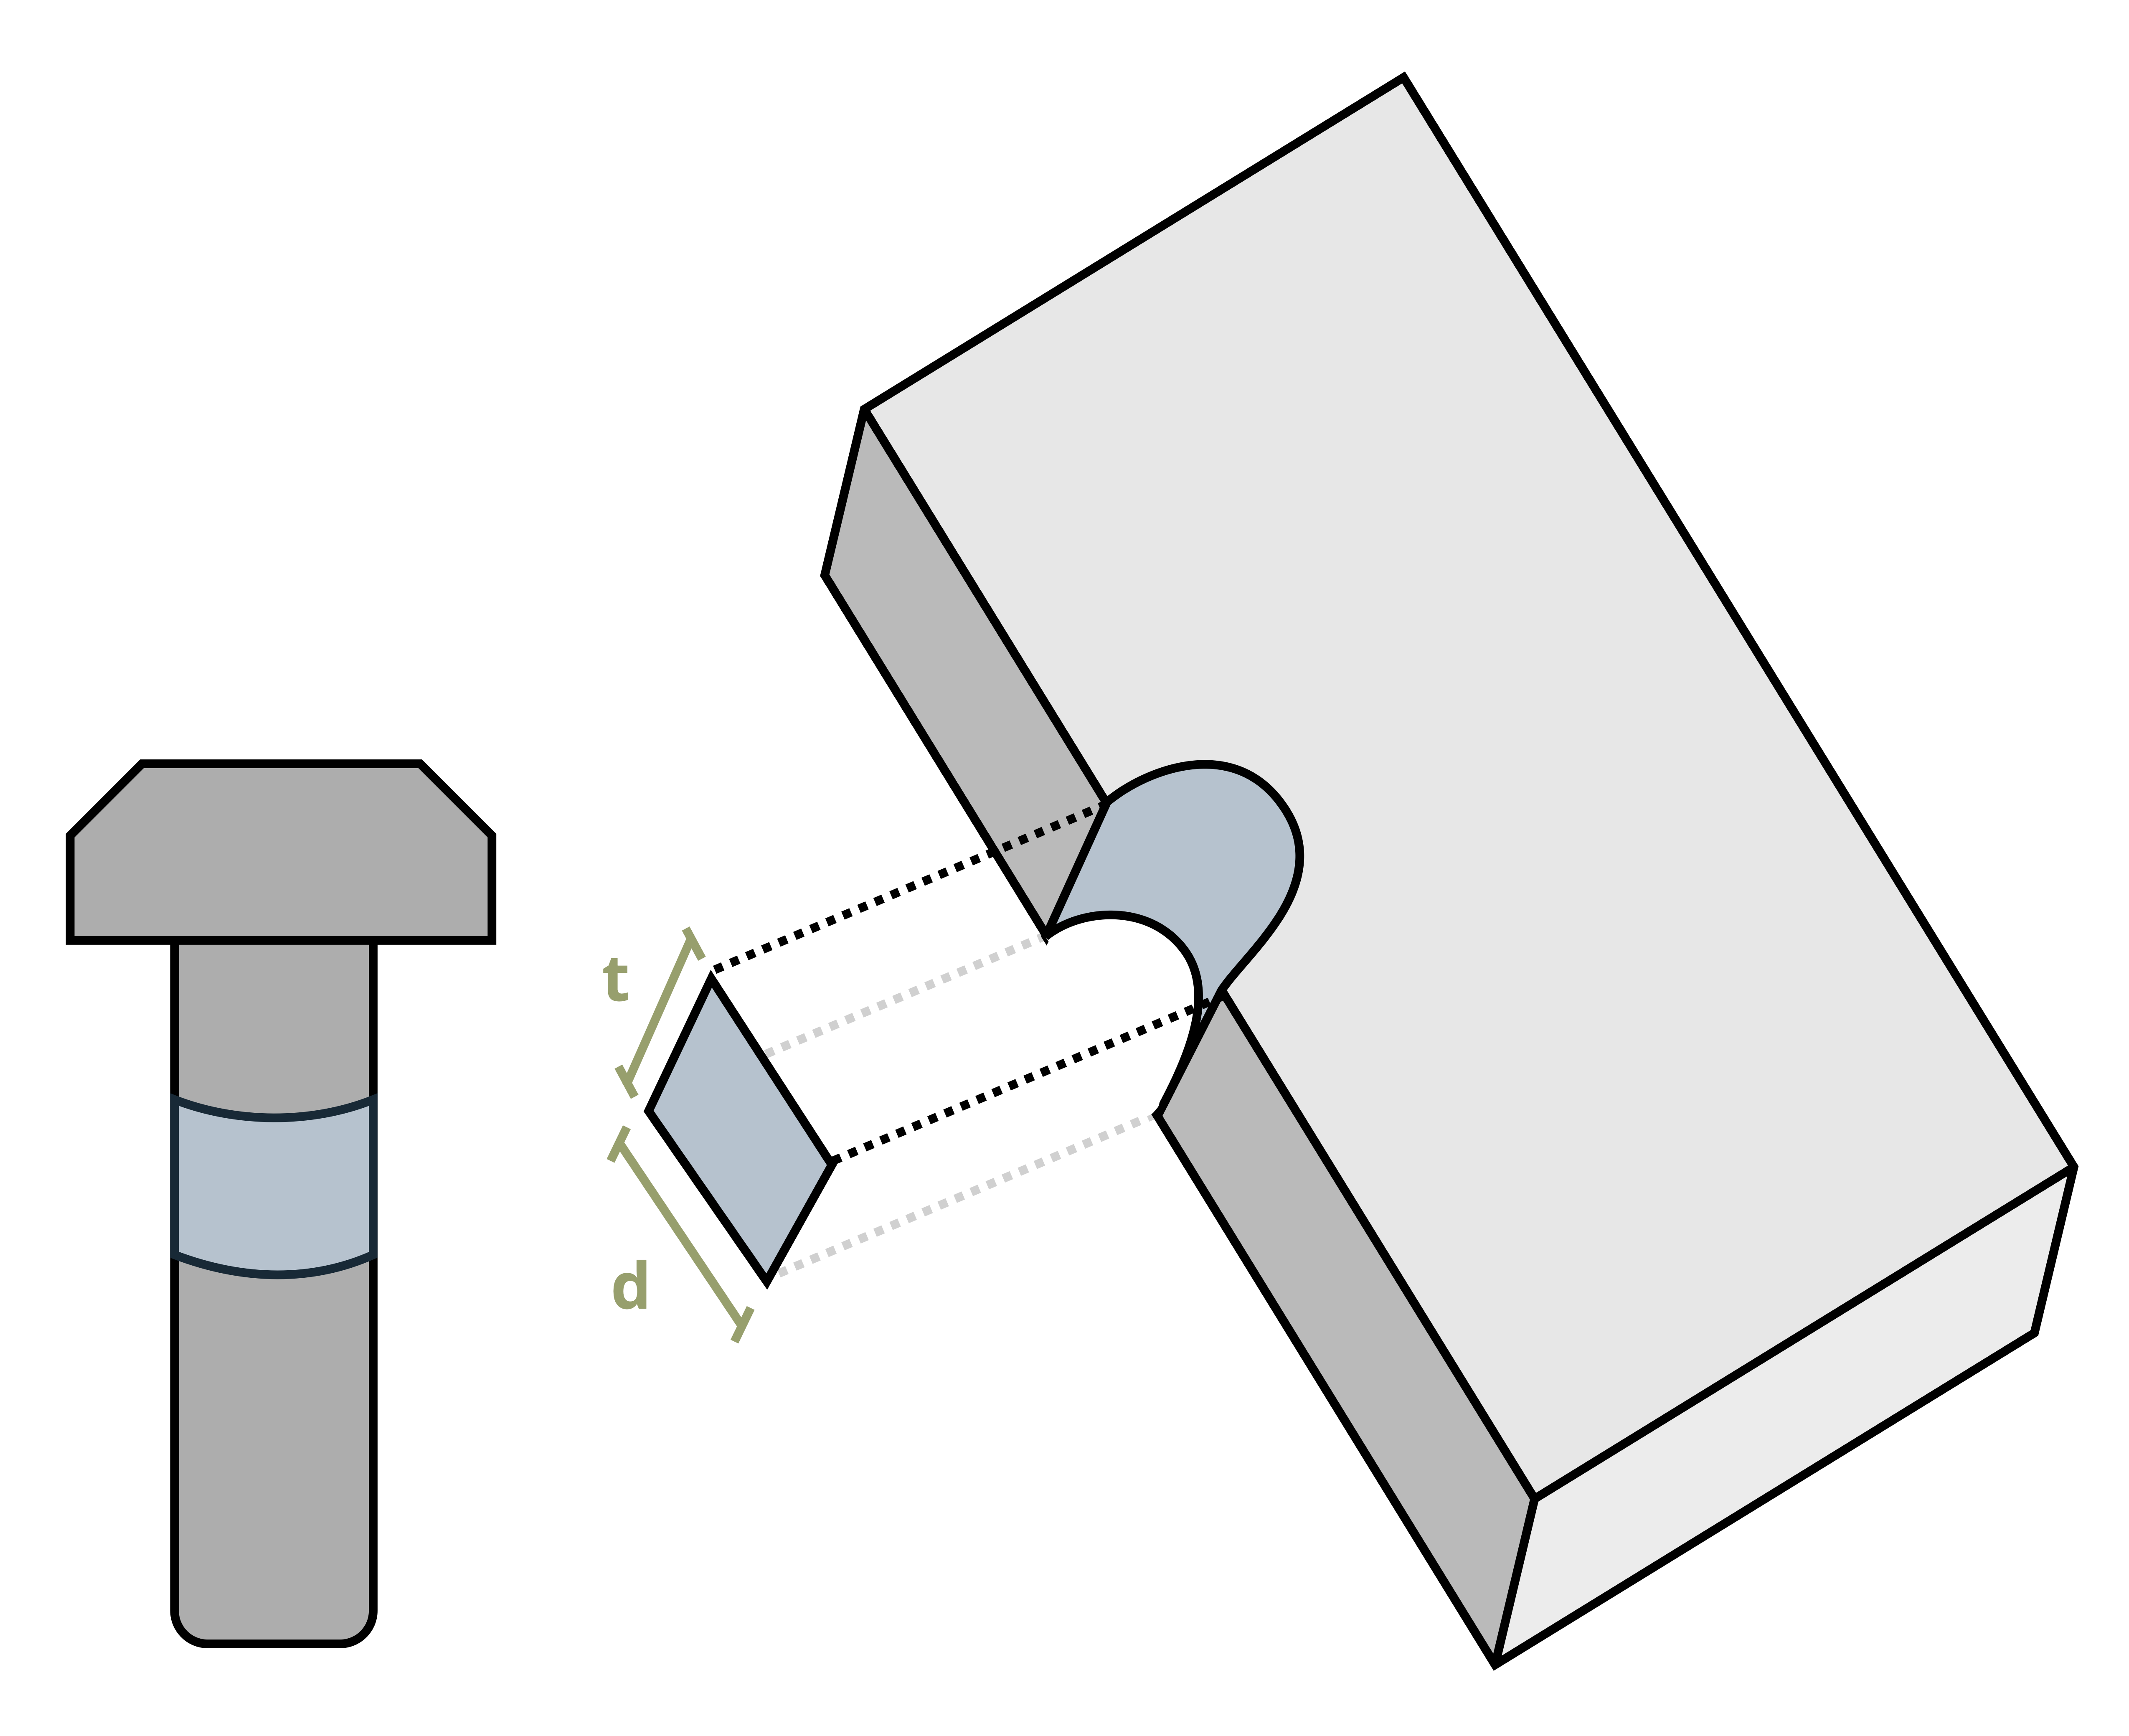
\includegraphics[width=4.23958in,height=\textheight]{images/CH2 figures/2.6.png}

}

\caption{\label{fig-2.6}When calculating the bearing stress between
curved surfaces, project a rectangle of area A = d*t.}

\end{figure}%

\begin{tcolorbox}[enhanced jigsaw, colback=white, colframe=quarto-callout-warning-color-frame, toptitle=1mm, arc=.35mm, bottomrule=.15mm, toprule=.15mm, opacitybacktitle=0.6, title={Step-by-step: Bearing Stress}, coltitle=black, breakable, colbacktitle=quarto-callout-warning-color!10!white, bottomtitle=1mm, titlerule=0mm, opacityback=0, leftrule=.75mm, left=2mm, rightrule=.15mm]

\begin{enumerate}
\def\labelenumi{\arabic{enumi}.}
\item
  Use equilibrium equations to determine reaction loads at any supports.
\item
  Determine the contact area between the two components (A).
\item
  Use equilibrium equations to determine the normal force (N) between
  the two components.
\item
  Determine average bearing stress using \(\sigma=\frac{N}{A}\).
\end{enumerate}

\end{tcolorbox}

\section{Stress on an Inclined Plane}\label{sec-2.4}

Click to expand

We have so far been cutting cross-sections perpendicular to the external
force, or parallel to it. However, there is no rule that says we have to
do this. It is perfectly acceptable to cut cross-sections at an angle
and there are many situations where it may make sense to do so
(Figure~\ref{fig-2.7}).

\begin{figure}

\centering{

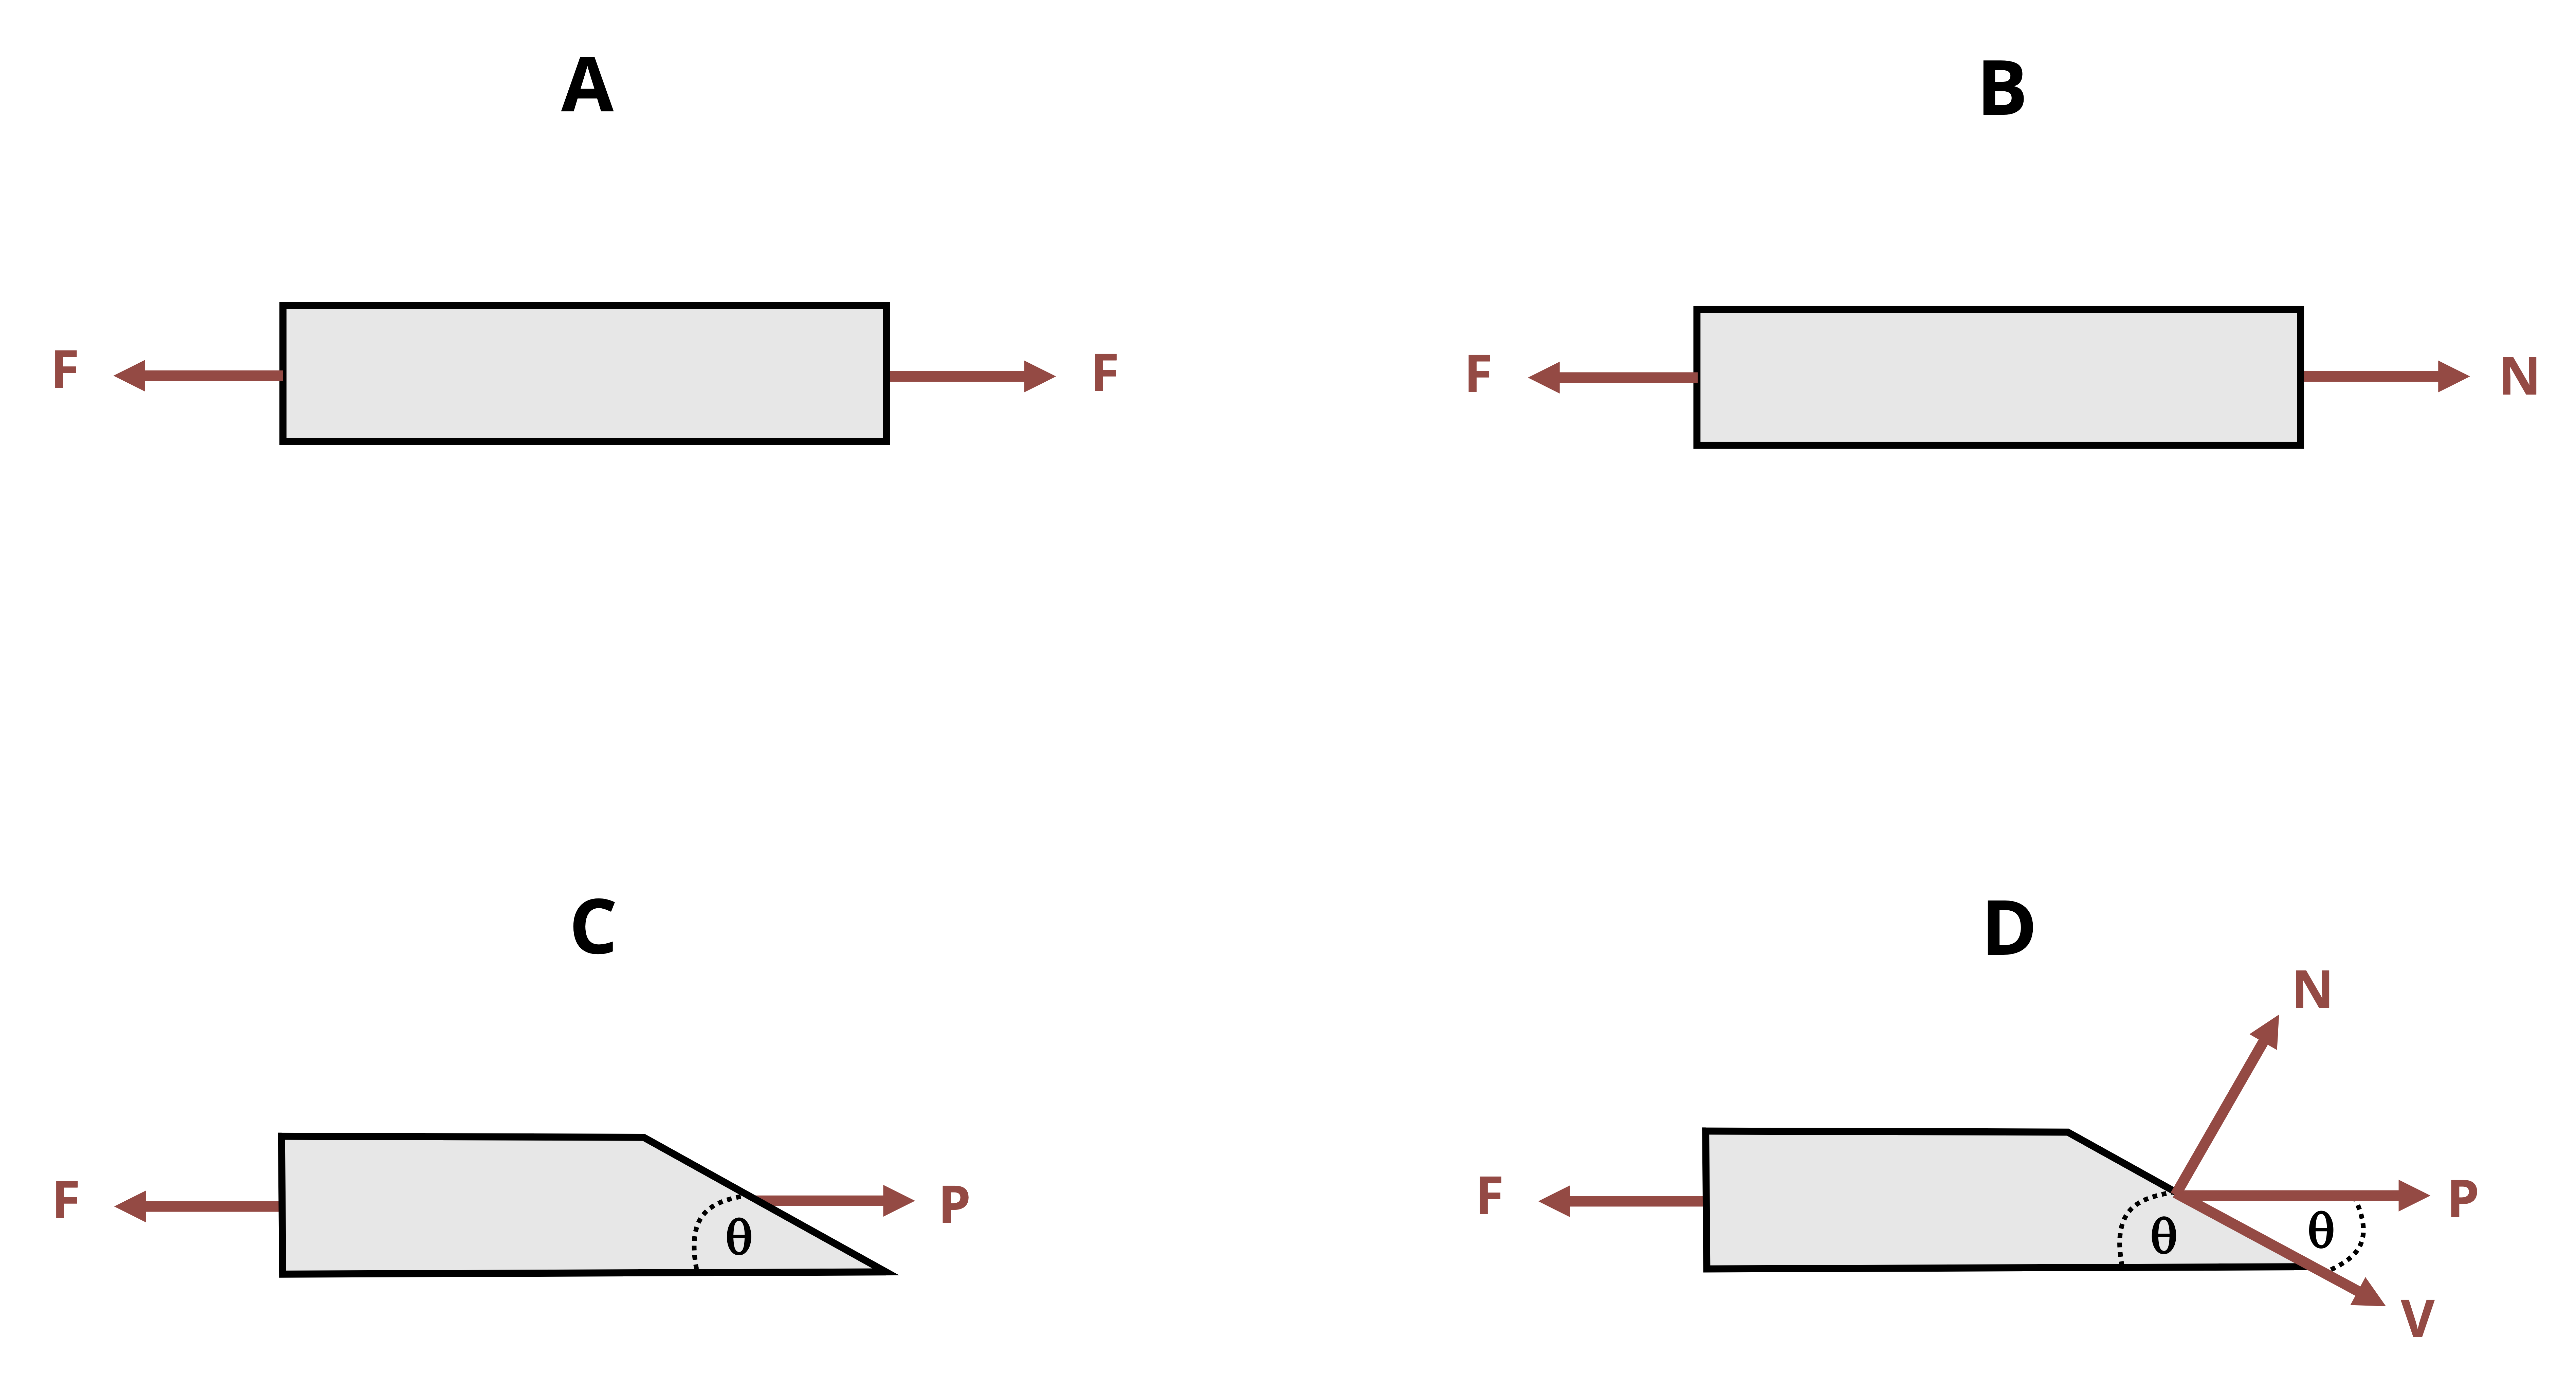
\includegraphics{images/CH2 figures/2.7.png}

}

\caption{\label{fig-2.7}(a) External loads, F, will create (b) an
internal normal force, N, when a cross-section is cut vertically. (c) If
the cross-section is cut along an inclined plane the internal force, P,
will not be a normal force or shear force. (d) The internal force should
be broken into normal (N) and shear (V) components that are
perpendicular and parallel to the plane respectively.}

\end{figure}%

In this scenario the internal load must still be equal and opposite to
the external load in order to maintain equilibrium but, because we cut
the cross-section at an angle, this internal load is neither parallel
nor perpendicular to the cross-section. Therefore it is not entirely a
normal force or a shear force. However, the internal force may be broken
into components that are perpendicular and parallel to the
cross-section.

\[
\begin{aligned}
& N=P \sin (\theta) \\
& V=P \cos (\theta)
\end{aligned}
\]

The area used to calculate the average normal and shear stresses must be
the area of the inclined plane (Figure~\ref{fig-2.8}). By setting up a
right-angled triangle it should be apparent that the area of the plane,
A\textsubscript{p}, can be found from:

\[
A_p=\frac{A}{\sin (\theta)}
\]

We can calculate average normal stress from:

\begin{equation}\phantomsection\label{eq-2.3}{\boxed{\sigma=\frac{N}{A_p}=\frac{P \sin (\theta)}{\frac{A}{\sin (\theta)}}=\frac{P \sin ^2(\theta)}{A}}}\end{equation}

We can calculate average shear stress from:

\begin{equation}\phantomsection\label{eq-2.4}{\boxed{\tau=\frac{V}{A_p}=\frac{P \cos (\theta)}{\frac{A}{\sin (\theta)}}=\frac{P \sin (\theta) \cos (\theta)}{A}}}\end{equation}

\emph{where}\\
\emph{𝜎 = Average normal stress on the inclined plane {[}Pa, psi{]}}\\
\emph{τ = Average shear stress on the inclined plane {[}Pa, psi{]}}\\
\emph{N = Internal normal force perpendicular to the inclined plane
{[}N, lb{]}}\\
\emph{V = Internal shear force perpendicular to the inclined plane {[}N,
lb{]}}\\
\emph{A\textsubscript{p} = Area of the inclined plane
{[}m\textsuperscript{2}, in.\textsuperscript{2}{]}}\\
\emph{A = Cross-sectional area {[}m\textsuperscript{2},
in\textsuperscript{2}{]}}\\
\emph{P = Internal load perpendicular to cross-sectional area A {[}N,
lb{]}}

\emph{𝜃 = Angle between the inclined plane and the axis perpendicular to
cross-sectional area A {[}°{]}}

Note these equations assume the angle (𝜃) is measured from the axis
perpendicular to area A. For a horizontal beam, area A is in the
vertical plane so angle θ is measured from the horizontal axis.

\begin{figure}

\centering{

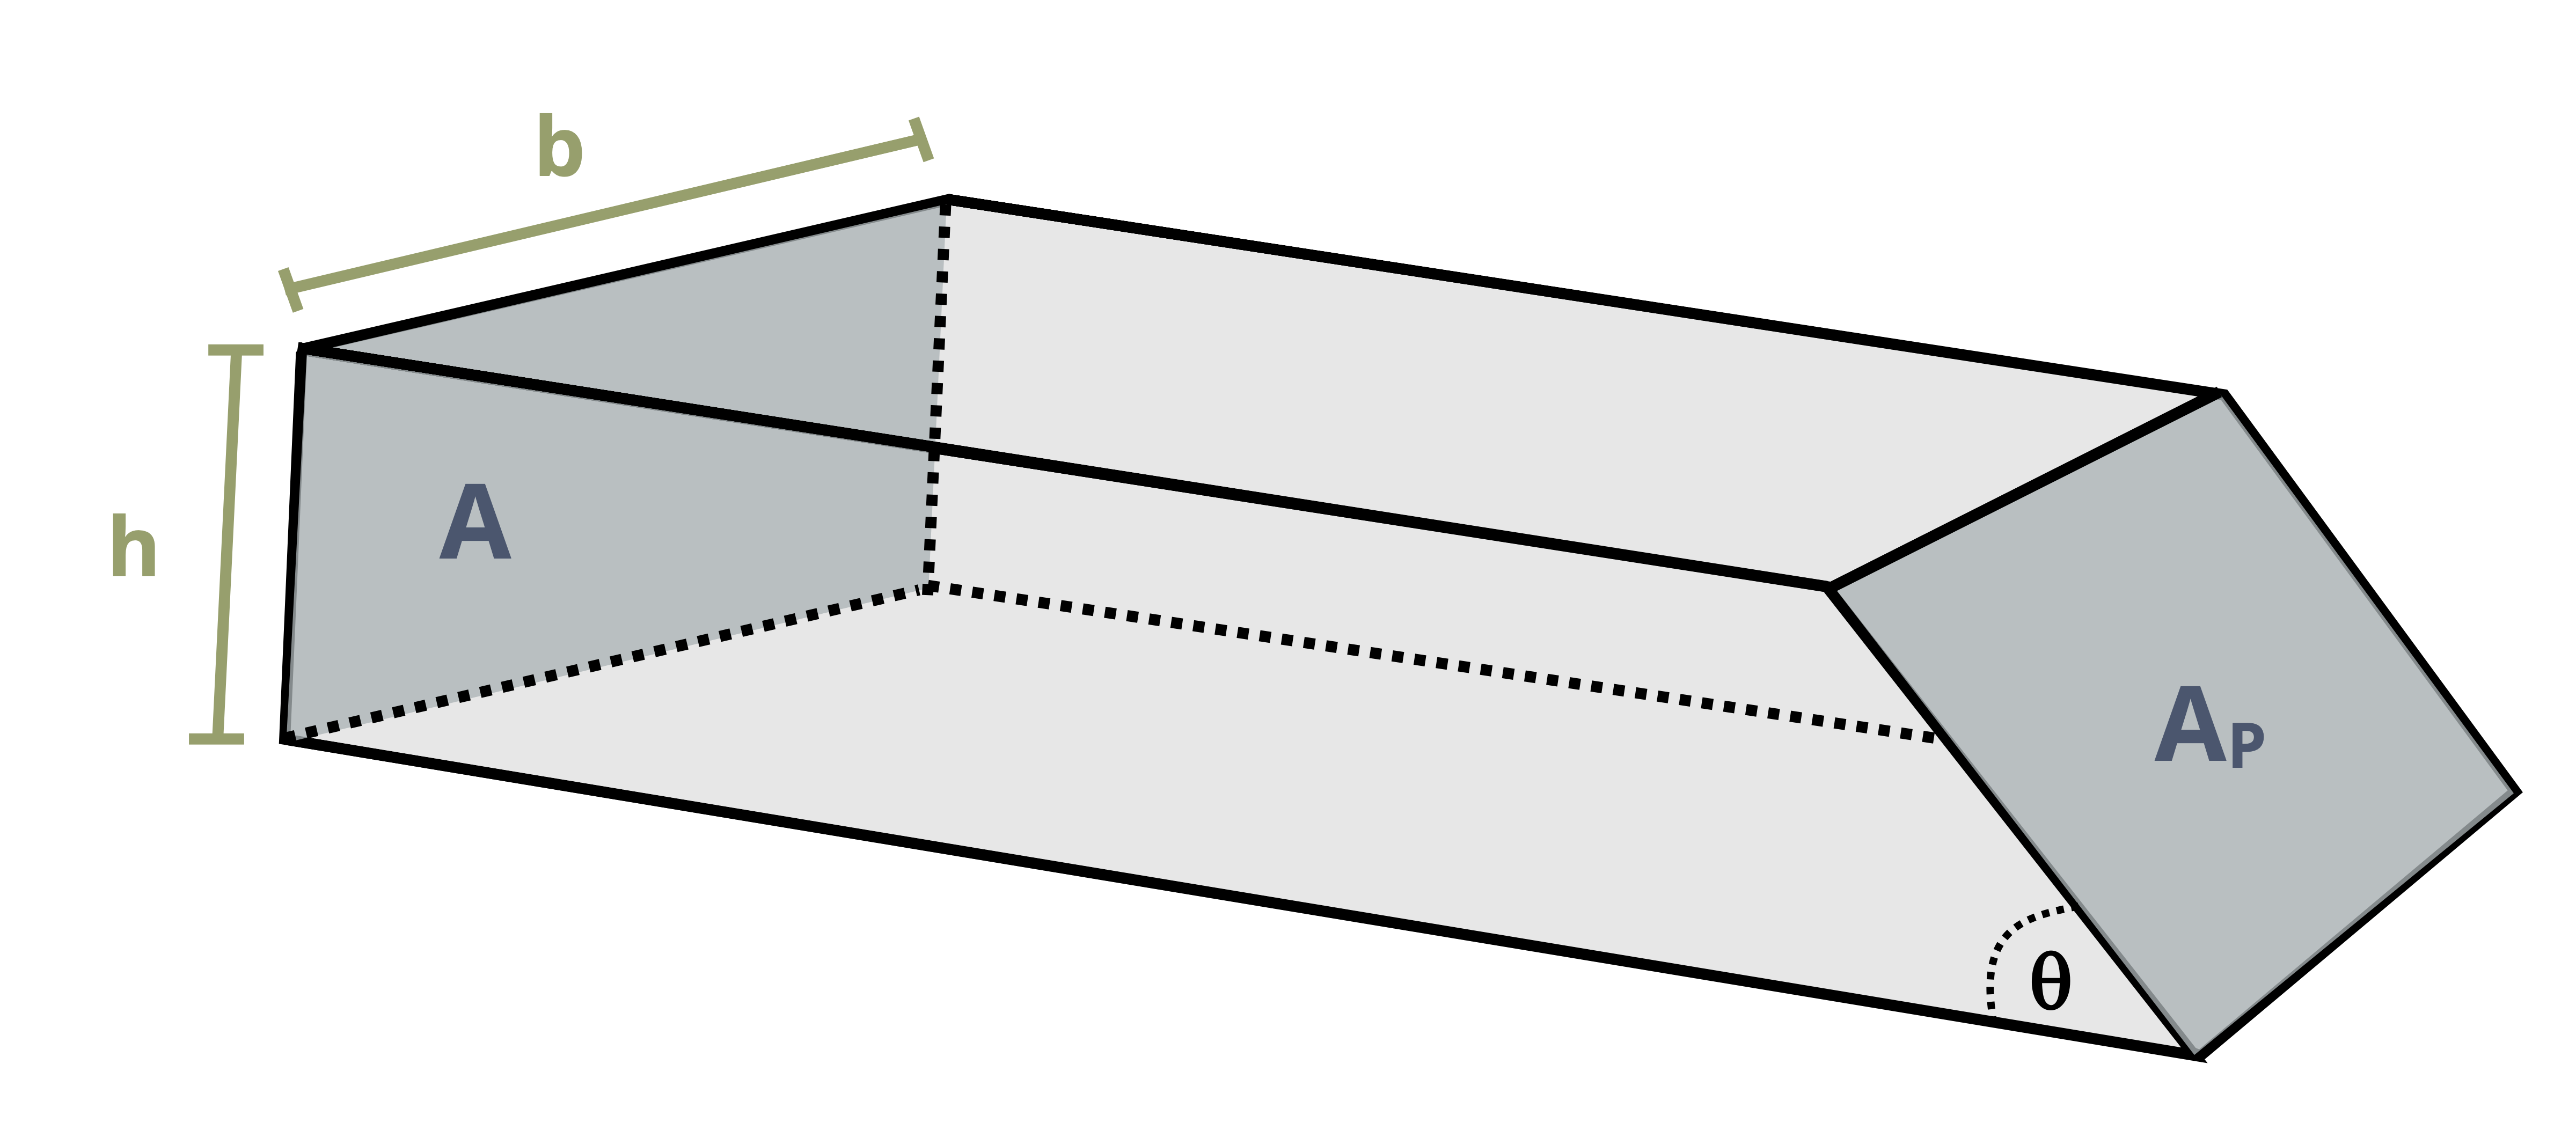
\includegraphics{images/CH2 figures/2.8.png}

}

\caption{\label{fig-2.8}When calculating the stresses on an inclined
plane, it is important to use the area of the plane, Ap, rather than the
area of the cross-sectional plane, A.}

\end{figure}%

Even if the external load remains constant, we can obtain different
values for the internal normal and shear forces (and therefore different
values for the stresses) by changing the angle at which we cut the
cross-section. We'll explore the implications of this further in
Chapter~\ref{sec-stress-transformation}. For now, a demonstration of
calculating the stresses on an inclined plane is given in
Example~\ref{exm-2.5}.

\begin{tcolorbox}[enhanced jigsaw, colback=white, colframe=quarto-callout-tip-color-frame, toptitle=1mm, arc=.35mm, bottomrule=.15mm, toprule=.15mm, opacitybacktitle=0.6, title={Example 2.5}, coltitle=black, breakable, colbacktitle=quarto-callout-tip-color!10!white, bottomtitle=1mm, titlerule=0mm, opacityback=0, leftrule=.75mm, left=2mm, rightrule=.15mm]

\begin{example}[]\protect\hypertarget{exm-2.5}{}\label{exm-2.5}

~

A beam is formed of two structural wooden members that are glued
together along an inclined plane at angle θ = 40° and subjected to a
tensile force of F = 30 kN. The height of the beam is 50 mm and its
thickness is 20 mm. Determine the normal and shear stresses created
along the inclined plane.

\begin{center}
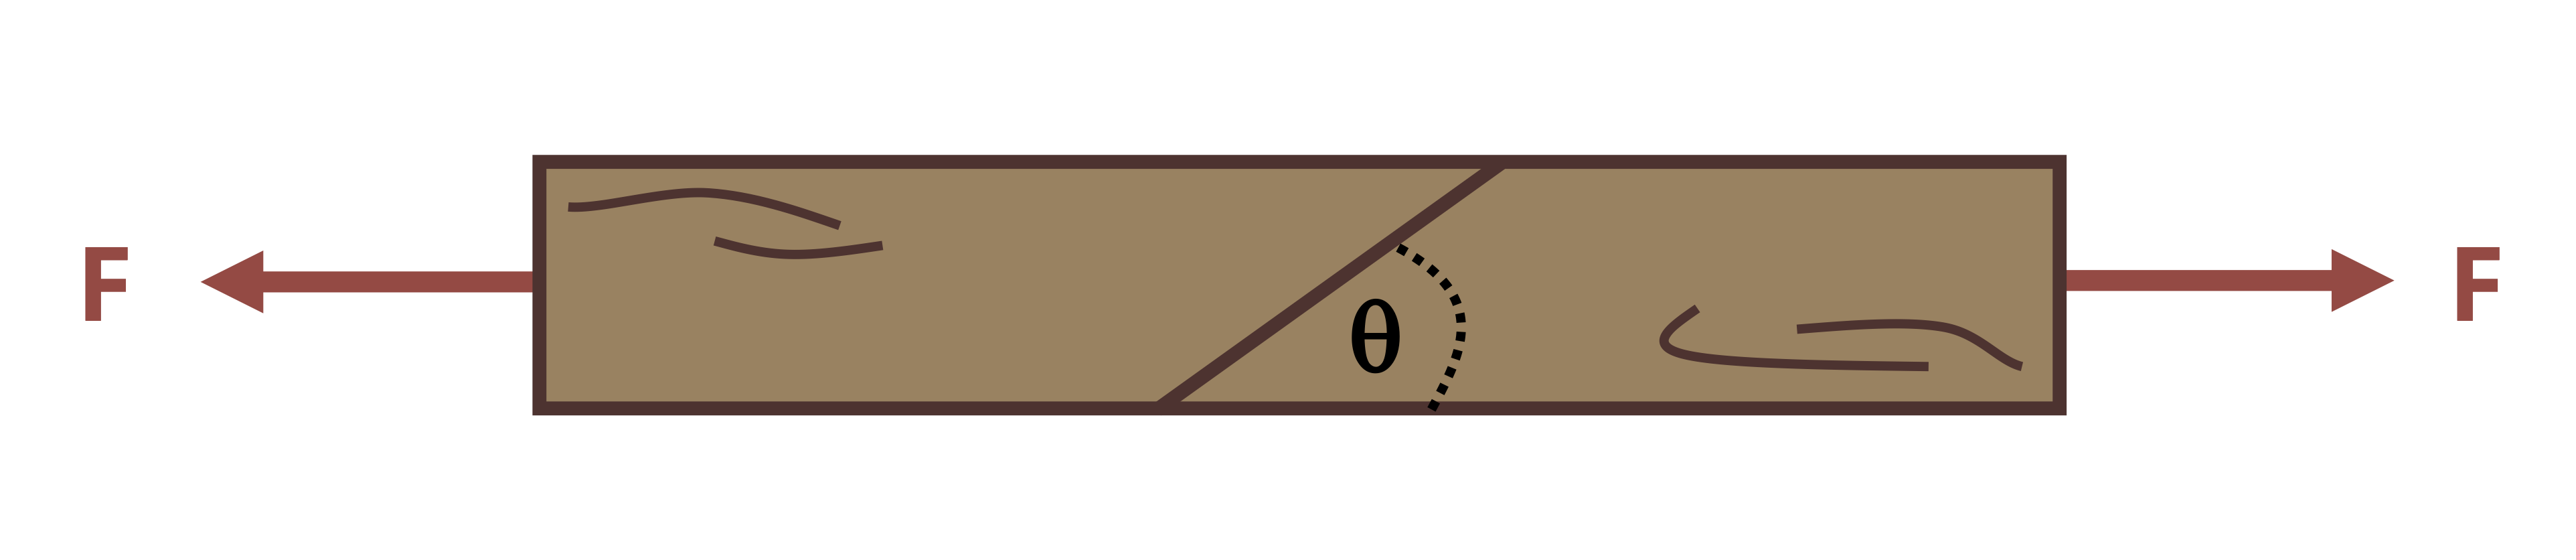
\includegraphics[width=3.0625in,height=\textheight]{images/CH2 figures/example 2.5 part 1.png}
\end{center}

\begin{tcolorbox}[enhanced jigsaw, colback=white, colframe=quarto-callout-tip-color-frame, toptitle=1mm, arc=.35mm, bottomrule=.15mm, toprule=.15mm, opacitybacktitle=0.6, title={Solution}, coltitle=black, breakable, colbacktitle=quarto-callout-tip-color!10!white, bottomtitle=1mm, titlerule=0mm, opacityback=0, leftrule=.75mm, left=2mm, rightrule=.15mm]

Begin by cutting a cross-section along the inclined plane and drawing a
free body diagram. Remember to include the internal normal and shear
forces perpendicular and parallel to the cross-section.

\begin{center}
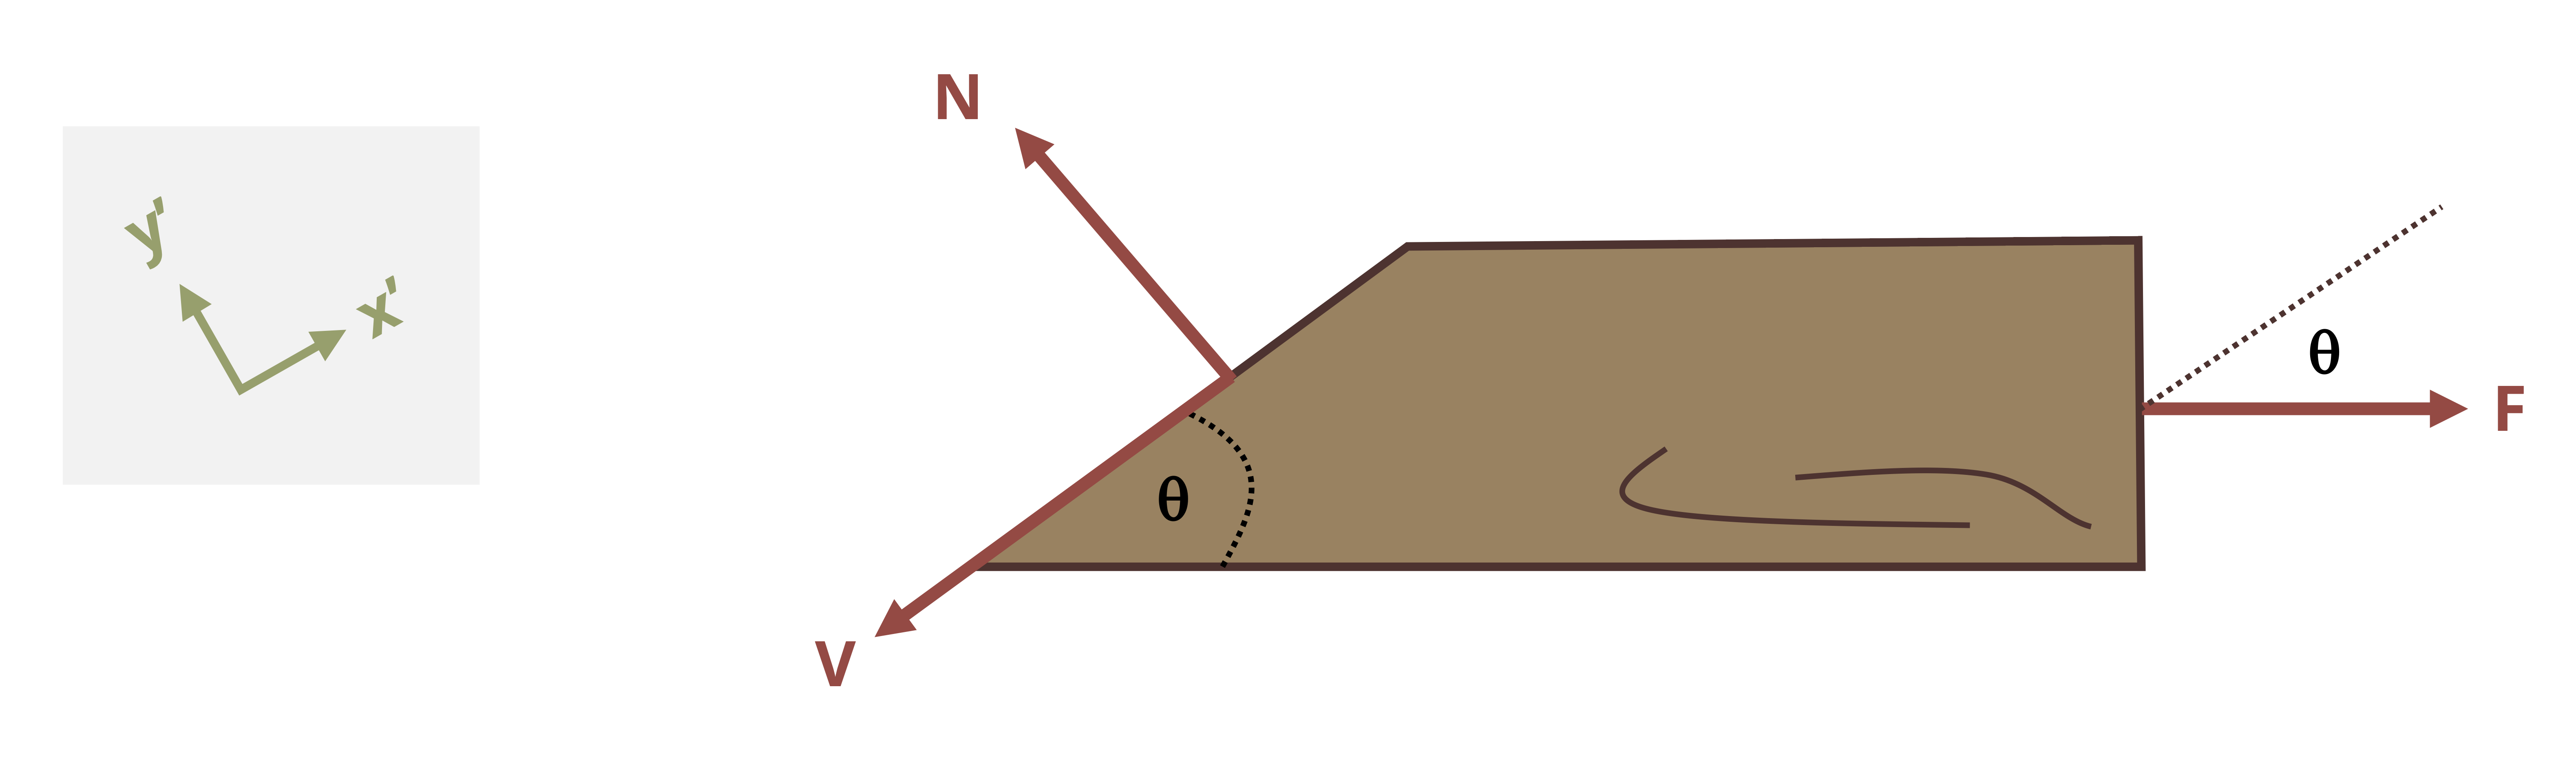
\includegraphics{images/CH2 figures/example 2.5 part 1 copy.png}
\end{center}

Use equilibrium equations to determine the internal forces. It will be
easiest to define axes parallel and perpendicular to the inclined plane.

\[
\begin{aligned}
\sum F_{x^{\prime}}= F \cos (\theta)-V=0 \\
\sum F_{y^{\prime}}= N-F \sin (\theta)=0
\end{aligned}
\]

With F = 30 kN and θ = 40°, these can be solved for N = 19.3 kN and V =
23.0 kN.

Next, determine the cross-sectional area of the inclined plane.

\[
A_p=\frac{A}{\sin (\theta)}
\]

With \(A = 0.05{~m}*0.02{~m} = 0.001{~m}^2\) and \(θ = 40°\),
\(Ap = 0.00156{~m}^2\).

Finally, determine the average normal stress and the average shear
stress.

\[
\begin{aligned}
\sigma & =\frac{N}{A_p}=\frac{19,300{~N}}{0.00156{~m}^2}=12.4 \times 10^6 \frac{{N}}{m^2}=12.4{~MPa} \\
\tau & =\frac{V}{A_p}=\frac{23,000{~N}}{0.00156{~m}^2}=14.8 \times 10^6 \frac{\mathrm{N}}{m^2}=14.8{~MPa}
\end{aligned}
\]

\end{tcolorbox}

\end{example}

\end{tcolorbox}

\begin{tcolorbox}[enhanced jigsaw, colback=white, colframe=quarto-callout-warning-color-frame, toptitle=1mm, arc=.35mm, bottomrule=.15mm, toprule=.15mm, opacitybacktitle=0.6, title={Step-by-step: Stresses on Inclined Planes}, coltitle=black, breakable, colbacktitle=quarto-callout-warning-color!10!white, bottomtitle=1mm, titlerule=0mm, opacityback=0, leftrule=.75mm, left=2mm, rightrule=.15mm]

\begin{enumerate}
\def\labelenumi{\arabic{enumi}.}
\item
  Use equilibrium equations to determine reaction loads at any supports.
\item
  Cut a cross-section along the inclined plane and determine the angle
  (θ) of the plane with respect to the axis perpendicular to
  cross-sectional area A.
\item
  Use equilibrium equations to determine the internal load (F).
\item
  Determine average normal stress using
  \(\sigma=\frac{F \sin ^2(\theta)}{A}\).
\item
  Determine average shear stress using
  \(\tau=\frac{F \sin (\theta) \cos (\theta)}{A}\).
\end{enumerate}

\end{tcolorbox}

\section*{Summary}\label{summary-1}
\addcontentsline{toc}{section}{Summary}

\markright{Summary}

Click to expand

\begin{tcolorbox}[enhanced jigsaw, colback=white, colframe=quarto-callout-note-color-frame, toptitle=1mm, arc=.35mm, bottomrule=.15mm, toprule=.15mm, opacitybacktitle=0.6, title={Key takeaways}, coltitle=black, breakable, colbacktitle=quarto-callout-note-color!10!white, bottomtitle=1mm, titlerule=0mm, opacityback=0, leftrule=.75mm, left=2mm, rightrule=.15mm]

Objects under load will experience stress. It is the stress level
(rather than just the load by itself) that determines whether an object
will break under load. We can calculate the average normal stress and
average shear stress acting on a body, though a complete understanding
of the stress field within a complex object often requires more advanced
concepts.

Stress depends on the internal load in the body, the cross-sectional
area, and the orientation of the plane. Normal stress occurs when there
is an internal normal force and may be tensile or compressive. Shear
stress occurs when there is an internal shear force. Members may
commonly experience multiple shear planes.

If there are multiple loads acting on a body, or if the body has
multiple cross-sectional areas at different points, different parts of
the body may experience different stresses. In such cases, we may
calculate the stress in each part of the body by finding the internal
load and cross-sectional area in that part of the body. In this chapter
we have discussed average stress. In subsequent chapters further details
on stress distributions will be discussed.

Bearing stress is similar to normal stress, but occurs between two
bodies.

We may calculate stresses along inclined planes by cutting a
cross-section at an angle. Determining the stresses at different angles
will be important later in our studies.

\end{tcolorbox}

\begin{tcolorbox}[enhanced jigsaw, colback=white, colframe=quarto-callout-note-color-frame, toptitle=1mm, arc=.35mm, bottomrule=.15mm, toprule=.15mm, opacitybacktitle=0.6, title={Key equations}, coltitle=black, breakable, colbacktitle=quarto-callout-note-color!10!white, bottomtitle=1mm, titlerule=0mm, opacityback=0, leftrule=.75mm, left=2mm, rightrule=.15mm]

Average normal stress:

\[
\sigma=\frac{N}{A}
\]

Average shear stress:

\[
\tau=\frac{V}{A}
\]

Bearing stress:

\[
\sigma=\frac{N}{A}
\]

Average stresses on an inclined plane:

\[
\begin{aligned}
\sigma & =\frac{P \sin ^2(\theta)}{A} \\
\tau & =\frac{P \sin (\theta) \cos (\theta)}{A}
\end{aligned}
\]

\end{tcolorbox}

\bookmarksetup{startatroot}

\chapter{Strain}\label{sec-strain}

\begin{tcolorbox}[enhanced jigsaw, colback=white, colframe=quarto-callout-note-color-frame, toptitle=1mm, arc=.35mm, bottomrule=.15mm, toprule=.15mm, opacitybacktitle=0.6, title={Learning Objectives}, coltitle=black, breakable, colbacktitle=quarto-callout-note-color!10!white, bottomtitle=1mm, titlerule=0mm, opacityback=0, leftrule=.75mm, left=2mm, rightrule=.15mm]

\begin{itemize}
\tightlist
\item
  Define strain
\item
  Explain the difference between normal strain and shear strain
\item
  Calculate normal and shear strains due to applied loads
\end{itemize}

\end{tcolorbox}

\section*{Introduction}\label{introduction-2}
\addcontentsline{toc}{section}{Introduction}

\markright{Introduction}

Click to expand

In Chapter~\ref{sec-stress} we learned how to calculate normal and shear
stresses with respect to a plane of interest, such as a cross-sectional
area or an inclined plane. If stresses get too large the object will
break, so it is important that engineers design structures and machines
such that the stresses stay within certain acceptable limits. It is also
important that objects do not deform so much that they are no longer fit
for their original purpose. Strain is a measure of the intensity of a
deformation---that is, the deformation per unit length.

Imagine two points on a body, A and B separated by some distance L
(Figure~\ref{fig-3.1}). In statics (and dynamics), objects are assumed
to be rigid and they do not deform when subjected to forces. In reality,
forces will cause an object to deform and its dimensions will change. As
points A and B move with the object, the distance between them will
change to some new distance L'.

\begin{figure}

\centering{

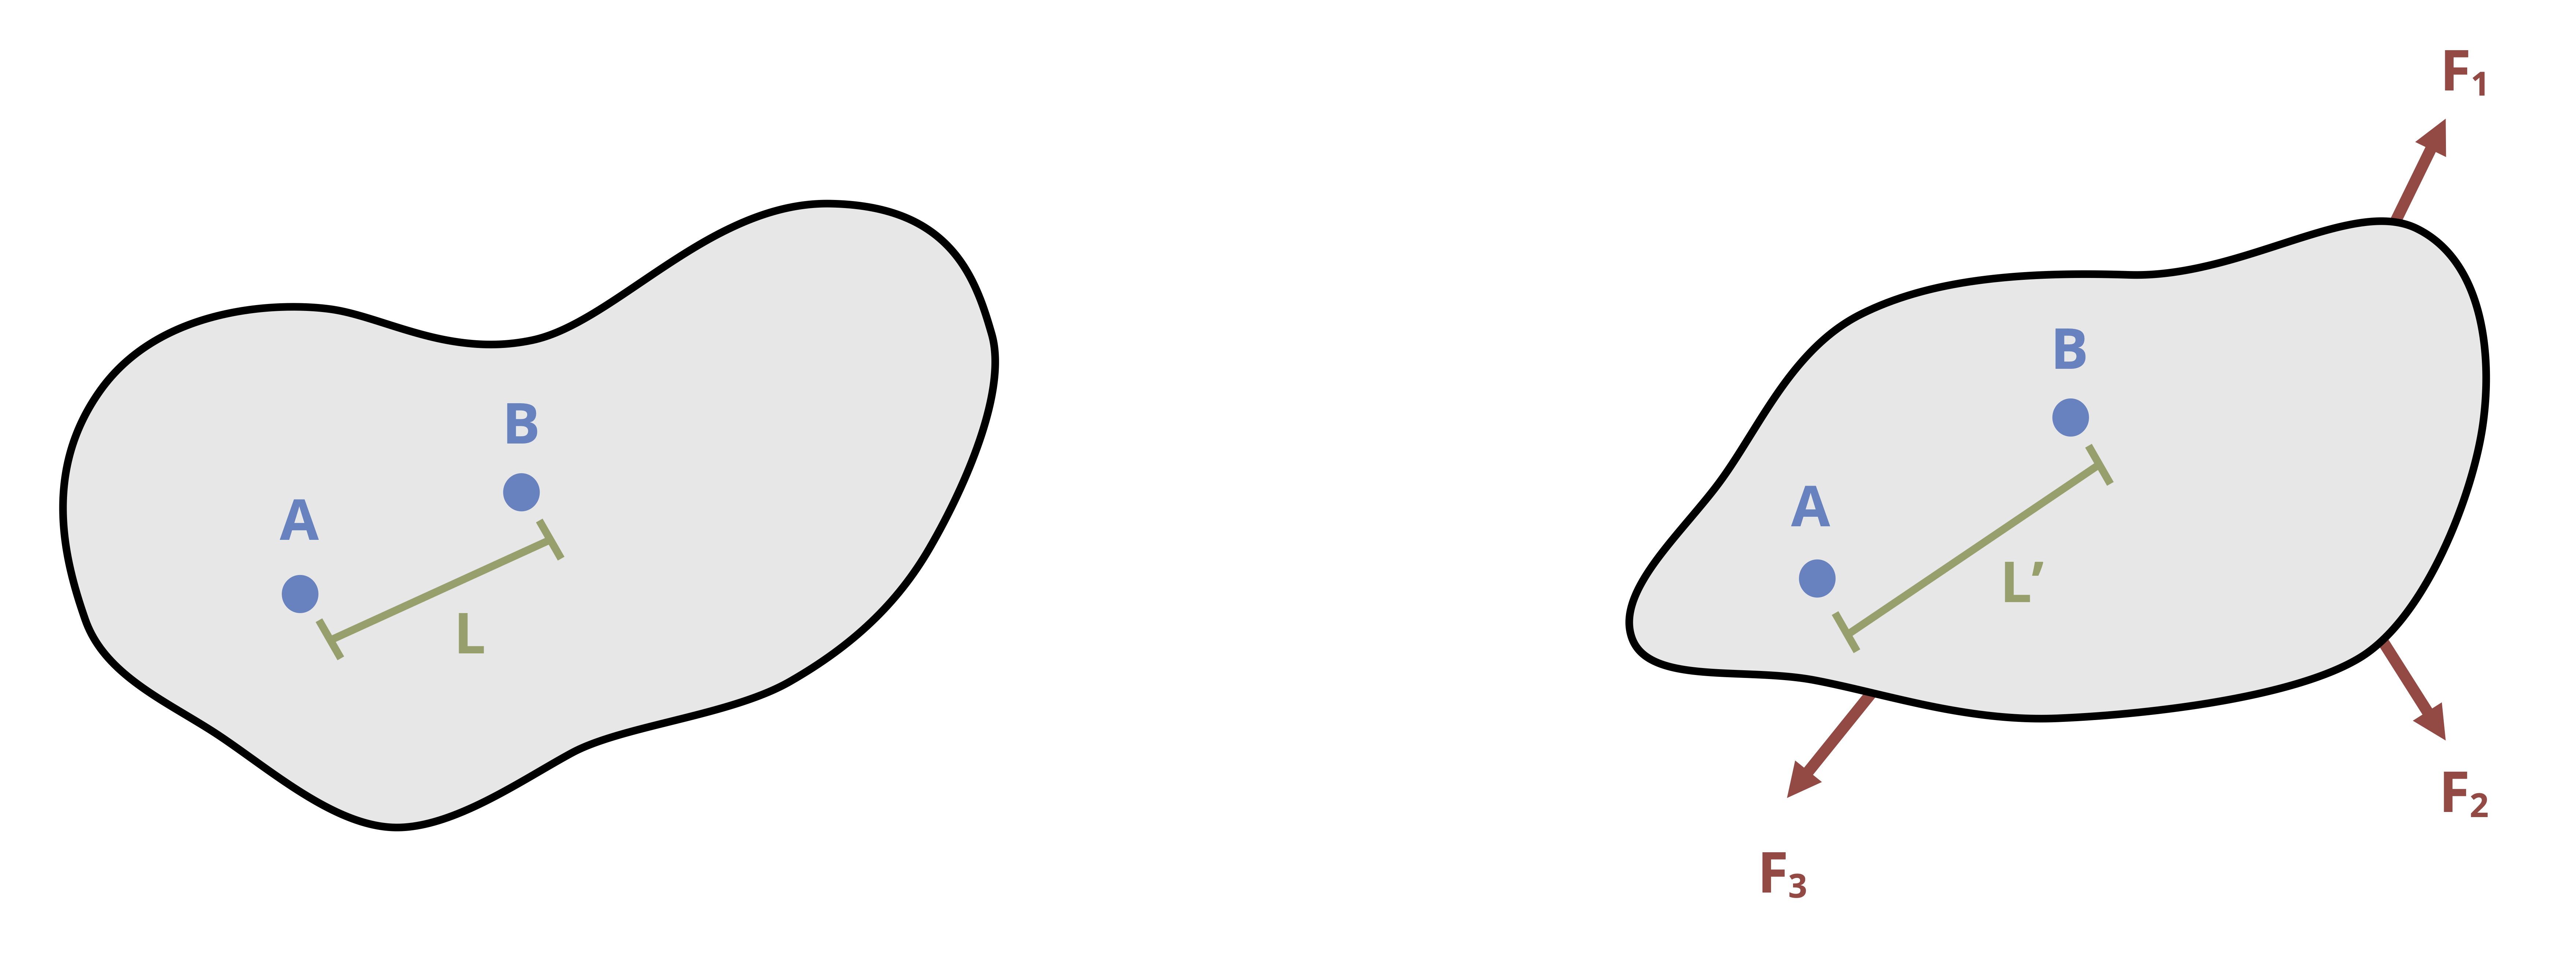
\includegraphics{images/CH3 PNGs/figure 3.1.png}

}

\caption{\label{fig-3.1}Nonrigid bodies will deform under load and the
distance between any two points A and B will change as the body
deforms.}

\end{figure}%

These deformations may be very large relative to the size of the object
(e.g., a rubber band) or they may be relatively small (e.g., structural
members) but there will always be some amount of deformation as no
material is infinitely stiff, as we will learn in
Chapter~\ref{sec-mechanical-properties-of-materials}. Engineers must
design structures and machines such that these deformations are not
excessively large for the intended application.

This chapter will introduce two types of strain. Section~\ref{sec-3.1}
covers normal strain which, like normal stress, occurs when objects are
subjected to axial loads. Section~\ref{sec-3.2} covers shear strain
which, like shear stress, occurs when objects are subjected to shear
loads.

\section{Normal Strain}\label{sec-3.1}

Click to expand

A simple example of normal strain is the deformation of a bar subjected
to an axial load. Consider a bar of length L subjected to a tensile
axial load P as shown in Figure~\ref{fig-3.2}. The load will create a
normal stress in the rod and will also cause the rod to elongate by an
amount ΔL.

\begin{figure}

\centering{

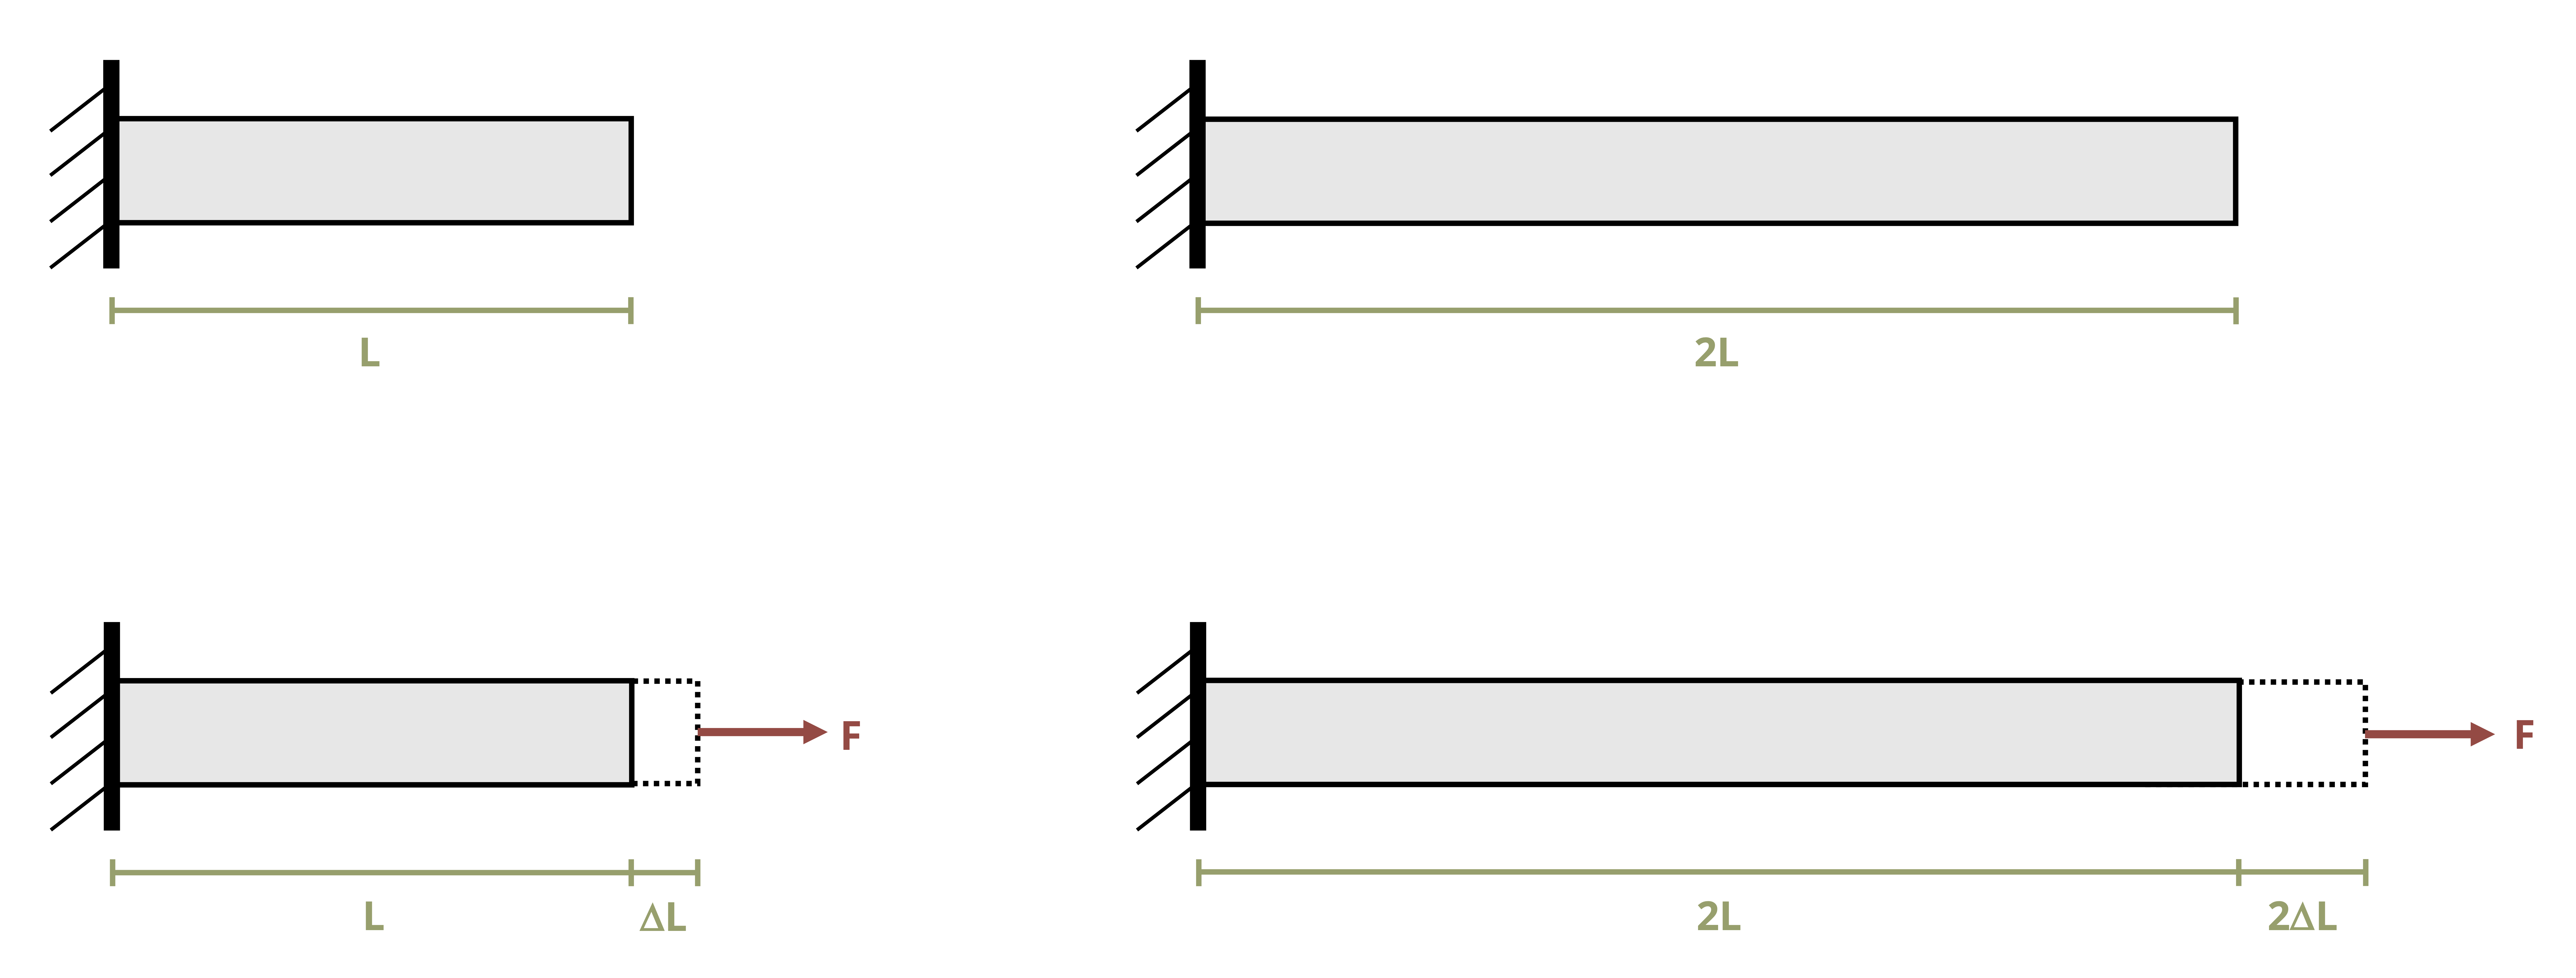
\includegraphics{images/CH3 PNGs/figure 3.2.png}

}

\caption{\label{fig-3.2}Axial loads cause a change in length that
depends partly on the original length of the object.}

\end{figure}%

If the same load were applied to a longer rod of length 2L with the same
cross-sectional area, the longer rod will elongate by an amount 2ΔL. The
deformation depends on the original length of the rod in this case, but
the strain does not. Strain is a measure that normalizes the change in
length by the original length. Normal strain is defined as:

\begin{equation}\phantomsection\label{eq-3.1}{
\boxed{\varepsilon=\frac{\Delta L}{L}}
}\end{equation}

\emph{where}\\
\emph{ε = Normal strain}\\
\emph{ΔL = Change in length {[}mm, in{]}}

\emph{L = Original length {[}mm, in{]}}

This is a normal strain because it occurs under axial load and is
associated with a change in length of the object. Since normal strain is
defined by dividing one length by another it does not have any units.
However, it is fairly common to still include units of mm/mm or in/in.

For example, if the rod was initially 5 m long and it elongated by 12
mm, the normal strain can be calculated as:

\[
\varepsilon=\frac{\Delta L}{L}=\frac{12}{5,000}=0.0024{~mm} /{mm}=0.0024
\]

Note that the units used for ΔL and L must be the same, but it does not
matter if they are expressed in mm or m. Using meters instead yields the
same answer:

\[
\varepsilon=\frac{\Delta L}{L}=\frac{0.012}{5}=0.0024{~m}/{m}=0.0024
\]

Because strains tend to be quite small in many engineering applications,
they are sometimes expressed with a prefix to eliminate the leading
zeros. For example, a strain of 0.0024 may be expressed as 2.4 mm/m or
2400 µm/m or simply 2400 µ. Strains may also be expressed as a
percentage, which can be found simply by multiplying the strain by
100\%. The below strains are all equivalent:

\[
\varepsilon=0.0024{~mm}/{mm}=0.0024{~m}/{m}=0.0024=2.4{~mm}/{m}=2400~\mu{m}/{m}=2400 ~\mu=0.24\%
\]

We will continue to use the sign convention that we defined for normal
stress. Tensile forces and stresses, which are associated with
elongation of the bar and tensile normal strain, are positive.
Compressive forces and stresses, which are associated with shortening of
the bar and compressive normal strain, are negative
(Figure~\ref{fig-3.3}).

\begin{figure}

\centering{

\includegraphics{images/CH3 PNGs/figure 3.3.png}

}

\caption{\label{fig-3.3}(A) Objects in tension will elongate. By
convention, tension and elongation are positive. (B) Objects in
compression will shorten. By convention, compression and shortening are
negative.}

\end{figure}%

See Example~\ref{exm-3.1} for a problem involving a bar experiencing
both tension and compression. Example~\ref{exm-3.2} involves strain in
two parallel cables.

\begin{tcolorbox}[enhanced jigsaw, colback=white, colframe=quarto-callout-tip-color-frame, toptitle=1mm, arc=.35mm, bottomrule=.15mm, toprule=.15mm, opacitybacktitle=0.6, title={Example 3.1}, coltitle=black, breakable, colbacktitle=quarto-callout-tip-color!10!white, bottomtitle=1mm, titlerule=0mm, opacityback=0, leftrule=.75mm, left=2mm, rightrule=.15mm]

\begin{example}[]\protect\hypertarget{exm-3.1}{}\label{exm-3.1}

~

The bar is subjected to forces F1 = 30 kips and F2 = 10 kips as shown.
Segment AB is originally 10 inches in length and segment BC is
originally 15 inches in length. As a result of the applied forces, the
normal strain in segment AB is -- 0.03 in/in and the strain in segment
BC is 0.045 in/in.

\begin{enumerate}
\def\labelenumi{\arabic{enumi}.}
\tightlist
\item
  Determine the change in length of each segment
\item
  Determine the overall strain for the entire bar
\end{enumerate}

\begin{center}
\includegraphics[width=3.03125in,height=\textheight]{images/CH3 PNGs/example 3.1.png}
\end{center}

\begin{tcolorbox}[enhanced jigsaw, colback=white, colframe=quarto-callout-tip-color-frame, toptitle=1mm, arc=.35mm, bottomrule=.15mm, toprule=.15mm, opacitybacktitle=0.6, title={Solution}, coltitle=black, breakable, colbacktitle=quarto-callout-tip-color!10!white, bottomtitle=1mm, titlerule=0mm, opacityback=0, leftrule=.75mm, left=2mm, rightrule=.15mm]

Using \(\varepsilon=\frac{\Delta L}{L}\) for each segment, rearrange to
calculate the change in length of each segment.

\[
\begin{aligned}
& \Delta L_{A B}=\varepsilon_{A B} L_{A B}=-0.03 * 10{~in.}=-0.3{~in.} \\
& \Delta L_{B C}=\varepsilon_{B C} L_{B C}=0.045 * 15{~in.}=0.675{~in.}
\end{aligned}
\]

To find the overall strain for the entire bar, first find the overall
change in length for the entire bar.

\[
\Delta L=-0.3{~in.}+0.675{~in.}=0.375{~in.}
\]

Overall, the bar elongates by 0.375 in. The original length of the bar
was 25 in. We can now determine the strain for the entire bar.

\[
\varepsilon=\frac{\Delta L}{L}=\frac{0.375{~in.}}{25{~in.}}=0.015{~in./in.}
\]

\end{tcolorbox}

\end{example}

\end{tcolorbox}

\begin{tcolorbox}[enhanced jigsaw, colback=white, colframe=quarto-callout-tip-color-frame, toptitle=1mm, arc=.35mm, bottomrule=.15mm, toprule=.15mm, opacitybacktitle=0.6, title={Example 3.2}, coltitle=black, breakable, colbacktitle=quarto-callout-tip-color!10!white, bottomtitle=1mm, titlerule=0mm, opacityback=0, leftrule=.75mm, left=2mm, rightrule=.15mm]

\begin{example}[]\protect\hypertarget{exm-3.2}{}\label{exm-3.2}

~

Rigid bar ABCD is supported by a pin at A and cables at B and D. After
load F is applied, the strain in cable D is 2300 µm/m. Determine the
strain in cable B.

\begin{center}
\includegraphics[width=3.38542in,height=\textheight]{images/CH3 PNGs/example 3.2 part 1.png}
\end{center}

\begin{tcolorbox}[enhanced jigsaw, colback=white, colframe=quarto-callout-tip-color-frame, toptitle=1mm, arc=.35mm, bottomrule=.15mm, toprule=.15mm, opacitybacktitle=0.6, title={Solution}, coltitle=black, breakable, colbacktitle=quarto-callout-tip-color!10!white, bottomtitle=1mm, titlerule=0mm, opacityback=0, leftrule=.75mm, left=2mm, rightrule=.15mm]

Consider the deflected position of rigid bar ABCD. We can calculate the
change in length of cable D.

\begin{center}
\includegraphics[width=3.63542in,height=\textheight]{images/CH3 PNGs/example 3.2 part 2.png}
\end{center}

\[
\Delta L_D=\varepsilon L=2300 \times 10^{-6} * 3.5{~m}=0.00805 {~m}=8.05 {~mm}
\]

Point D will deflect downwards by 8.05 mm. Use similar triangles to find
the deflection of point B.

\[
\begin{gathered}
\frac{\Delta L_B}{6{~m}}=\frac{8.05{~mm}}{11{~m}} \\
\Delta L_B=\frac{6{~m} * 8.05{~mm}}{11{~m}}=4.39{~mm}
\end{gathered}
\]

Cable B will elongate by 4.39 mm. Use this to determine the strain in
cable B. Be careful to be consistent with units. Either use ΔL = 4.39 mm
and L = 2000 mm, or ΔL = 0.00439 m and L = 2 m.

\[
\varepsilon=\frac{\Delta L}{L}=\frac{4.39{~mm}}{2000{~mm}}=0.002195{~m}/{m}=2195 ~\mu{m} /{m}
\]

\end{tcolorbox}

\end{example}

\end{tcolorbox}

\begin{tcolorbox}[enhanced jigsaw, colback=white, colframe=quarto-callout-warning-color-frame, toptitle=1mm, arc=.35mm, bottomrule=.15mm, toprule=.15mm, opacitybacktitle=0.6, title={Step-by-step: Normal strain}, coltitle=black, breakable, colbacktitle=quarto-callout-warning-color!10!white, bottomtitle=1mm, titlerule=0mm, opacityback=0, leftrule=.75mm, left=2mm, rightrule=.15mm]

\begin{enumerate}
\def\labelenumi{\arabic{enumi}.}
\tightlist
\item
  Determine the change in length of the object
\item
  Calculate the normal strain, \(\varepsilon=\frac{\Delta L}{L}\)
\end{enumerate}

\end{tcolorbox}

\section{Shear Strain}\label{sec-3.2}

Click to expand

Consider a small, square element that may be part of a body such as that
shown in Figure~\ref{fig-3.1}. As well as the distance between points
changing as the body deforms, the shape of this square element will also
change. The corners of the square element will initially form
right-angles. As the body deforms and the points move with the object,
the shape of the element changes and the corners no longer form
right-angles (Figure~\ref{fig-3.4}).

\begin{figure}

\centering{

\includegraphics{images/CH3 PNGs/figure 3.4.png}

}

\caption{\label{fig-3.4}(A) The undeformed element is initially square,
with right-angled corners. (B) As the body deforms, the square element
skews and the corners are no longer right-angles.}

\end{figure}%

While normal strain represents a change in length, a shear strain
represents a change in angle---a distortion of the shape. Specifically,
provided we start with right-angled corners, shear strain is defined as
the original angle (before deformation) minus the new angle (after
deformation). Regardless of the shape of the body, a square element can
always be defined such that the original angle is always a right angle.
After deformation, the new angle between these three points is 𝜃'. Shear
strain is given the symbol γ and is, like normal strain, a dimensionless
quantity, so is represented in radians (not degrees). Thus the original
right angle is represented as \(\frac{\pi}{2}\) radians and the shear
strain as:

\begin{equation}\phantomsection\label{eq-3.2}{
\boxed{\gamma=\frac{\pi}{2}-\theta^{\prime}}
}\end{equation}

\emph{where}\\
\emph{𝛾 = Shear strain {[}rad{]}}\\
\(\frac{\pi}{2}\) \emph{= Original angle {[}rad{]}}

\emph{𝜃' = New angle {[}rad{]}}

Since we always subtract the new angle from the original angle, note
that if the angle increases we get a negative shear strain and if the
angle decreases we get a positive shear strain (Figure~\ref{fig-3.5}).

\begin{figure}

\centering{

\includegraphics[width=5.05208in,height=\textheight]{images/CH3 PNGs/figure 3.5.png}

}

\caption{\label{fig-3.5}(A) If the new angle 𝜃' is larger than
\(\frac{\pi}{2}\) radians, the shear strain is negative. (B) If the new
angle 𝜃' is smaller than \(\frac{\pi}{2}\) radians, the shear strain is
positive.}

\end{figure}%

See Example~\ref{exm-3.3} and Example~\ref{exm-3.4} to practice
calculating shear strain.

\begin{tcolorbox}[enhanced jigsaw, colback=white, colframe=quarto-callout-tip-color-frame, toptitle=1mm, arc=.35mm, bottomrule=.15mm, toprule=.15mm, opacitybacktitle=0.6, title={Example 3.3}, coltitle=black, breakable, colbacktitle=quarto-callout-tip-color!10!white, bottomtitle=1mm, titlerule=0mm, opacityback=0, leftrule=.75mm, left=2mm, rightrule=.15mm]

\begin{example}[]\protect\hypertarget{exm-3.3}{}\label{exm-3.3}

~

A thin rectangular plate has a base of 300 mm and a height of 500 mm.
Initially corners A, B, C, and D are all right-angles. The plate is
subjected to a shear force V which deforms the plate into the dotted
lines shown. Corner D moves straight downward by 5 mm. Determine the
shear strain at corner A.

\begin{center}
\includegraphics[width=2.95833in,height=\textheight]{images/CH3 PNGs/example 3.3 part 1.png}
\end{center}

\begin{tcolorbox}[enhanced jigsaw, colback=white, colframe=quarto-callout-tip-color-frame, toptitle=1mm, arc=.35mm, bottomrule=.15mm, toprule=.15mm, opacitybacktitle=0.6, title={Solution}, coltitle=black, breakable, colbacktitle=quarto-callout-tip-color!10!white, bottomtitle=1mm, titlerule=0mm, opacityback=0, leftrule=.75mm, left=2mm, rightrule=.15mm]

We could calculate the new angle at corner A as
\(\theta^{\prime}=\frac{\pi}{2}+\alpha\).

\begin{center}
\includegraphics[width=2.84375in,height=\textheight]{images/CH3 PNGs/example 3.3 part 2.png}
\end{center}

Angle α can be found since there is a triangle of base 300 mm and height
5 mm.

\[
\alpha=\tan ^{-1}\left(\frac{5}{300}\right)=0.01667 {~rad}
\]

Then:

\[
\theta^{\prime}=\frac{\pi}{2}+0.01667{~rad}=1.5875 {~rad}
\]

Now the shear strain can be calculated:

\[
\gamma=\frac{\pi}{2}-\theta^{\prime}=\frac{\pi}{2}-1.5875{~rad}=-0.01667 {~rad}
\]

Notice that this is just the negative of angle α. Since the shear strain
is the change in angle and α represents the increase of the angle, we
could have simply said that angle α is the shear strain. As defined in
Section~\ref{sec-3.2}, the shear strain is negative because the angle is
increasing.

\end{tcolorbox}

\end{example}

\end{tcolorbox}

\begin{tcolorbox}[enhanced jigsaw, colback=white, colframe=quarto-callout-tip-color-frame, toptitle=1mm, arc=.35mm, bottomrule=.15mm, toprule=.15mm, opacitybacktitle=0.6, title={Example 3.4}, coltitle=black, breakable, colbacktitle=quarto-callout-tip-color!10!white, bottomtitle=1mm, titlerule=0mm, opacityback=0, leftrule=.75mm, left=2mm, rightrule=.15mm]

\begin{example}[]\protect\hypertarget{exm-3.4}{}\label{exm-3.4}

~

A thin triangular plate ABC has a base of 8 inches and a height of 20
inches. Corner A is initially a right-angle. When subjected to a shea
load, the plate deforms as shown. Corner B moves 0.1 inches to the right
and corner C moves 0.06 inches downward. Determine the shear strain at
corner A.

\begin{center}
\includegraphics[width=3.33333in,height=\textheight]{images/CH3 PNGs/example 3.4 part 1.png}
\end{center}

\begin{tcolorbox}[enhanced jigsaw, colback=white, colframe=quarto-callout-tip-color-frame, toptitle=1mm, arc=.35mm, bottomrule=.15mm, toprule=.15mm, opacitybacktitle=0.6, title={Solution}, coltitle=black, breakable, colbacktitle=quarto-callout-tip-color!10!white, bottomtitle=1mm, titlerule=0mm, opacityback=0, leftrule=.75mm, left=2mm, rightrule=.15mm]

The angle at A will decrease by angle α and increase by angle β. Start
by finding these angles.

\begin{center}
\includegraphics[width=2.40625in,height=\textheight]{images/CH3 PNGs/example 3.4 part 2.png}
\end{center}

\[
\begin{gathered}
\alpha=\tan ^{-1}\left(\frac{0.1}{20}\right)=0.005{~rad} \\
\beta=\tan ^{-1}\left(\frac{0.06}{8}\right)=0.0075{~rad}
\end{gathered}
\]

The new angle at A will be:

\[
\theta^{\prime}=\frac{\pi}{2}-\alpha+\beta=1.5708-0.005+0.0075=1.5733{~rad}
\]

With the new angle known, we can calculate the shear strain.

\[
\gamma=\frac{\pi}{2}-1.5733{~rad}=-0.0025{~rad}
\]

Note that we could have calculated the shear strain more directly. Since
shear strain is just the change in angle, we could have said that the
angle at A decreases by angle α and increases by angle β.

Recall that shear strain is positive if the angle decreases and negative
if the angle increases. The change in angle at A, and thus the shear
strain, could be calculated as:

\[
\gamma=\alpha-\beta=0.005{~rad}-0.0075{~rad}=-0.0025{~rad}
\]

\end{tcolorbox}

\end{example}

\end{tcolorbox}

\begin{tcolorbox}[enhanced jigsaw, colback=white, colframe=quarto-callout-warning-color-frame, toptitle=1mm, arc=.35mm, bottomrule=.15mm, toprule=.15mm, opacitybacktitle=0.6, title={Step-by-step: Shear strain}, coltitle=black, breakable, colbacktitle=quarto-callout-warning-color!10!white, bottomtitle=1mm, titlerule=0mm, opacityback=0, leftrule=.75mm, left=2mm, rightrule=.15mm]

\begin{enumerate}
\def\labelenumi{\arabic{enumi}.}
\tightlist
\item
  Begin with a corner that forms a right-angle (\(\frac{\pi}{2}\) rads)
  prior to deformation
\item
  After deformation, determine the new angle (𝜃') at this corner
\item
  Determine the shear strain, \(\gamma=\frac{\pi}{2}-\theta^{\prime}\)
\end{enumerate}

\end{tcolorbox}

\section*{Summary}\label{summary-2}
\addcontentsline{toc}{section}{Summary}

\markright{Summary}

Click to expand

\begin{tcolorbox}[enhanced jigsaw, colback=white, colframe=quarto-callout-note-color-frame, toptitle=1mm, arc=.35mm, bottomrule=.15mm, toprule=.15mm, opacitybacktitle=0.6, title={Key takeaways}, coltitle=black, breakable, colbacktitle=quarto-callout-note-color!10!white, bottomtitle=1mm, titlerule=0mm, opacityback=0, leftrule=.75mm, left=2mm, rightrule=.15mm]

Objects may experience a change in length, for example due to axial
loads. If the load is tensile, the length will increase. If the load is
compressive, the length will decrease.

Normal strain is defined as the change in length divided by the original
length. Strain has no units, but is commonly written with units of mm/mm
or in./in. or similar. Normal strain is positive if the length increases
and negative if the length decreases.

Objects subjected to shear loads will experience a change in angle.
Shear strain is defined as this change in angle, expressed as original
angle -- new angle, where the original angle is always a right-angle.
Shear strains are positive if the angle decreases and negative if the
angle increases.

Shear strains are expressed in radians, not degrees, and so the original
angle is always defined as \(\frac{\pi}{2}\) radians.

\end{tcolorbox}

\begin{tcolorbox}[enhanced jigsaw, colback=white, colframe=quarto-callout-note-color-frame, toptitle=1mm, arc=.35mm, bottomrule=.15mm, toprule=.15mm, opacitybacktitle=0.6, title={Key equations}, coltitle=black, breakable, colbacktitle=quarto-callout-note-color!10!white, bottomtitle=1mm, titlerule=0mm, opacityback=0, leftrule=.75mm, left=2mm, rightrule=.15mm]

Normal strain:

\[
\varepsilon=\frac{\Delta L}{L}
\]

Shear strain:

\[
\gamma=\frac{\pi}{2}-\theta^{\prime}
\]

\end{tcolorbox}

\bookmarksetup{startatroot}

\chapter{Mechanical Properties of
Materials}\label{sec-mechanical-properties-of-materials}

\begin{tcolorbox}[enhanced jigsaw, colback=white, colframe=quarto-callout-note-color-frame, toptitle=1mm, arc=.35mm, bottomrule=.15mm, toprule=.15mm, opacitybacktitle=0.6, title={Learning Objectives}, coltitle=black, breakable, colbacktitle=quarto-callout-note-color!10!white, bottomtitle=1mm, titlerule=0mm, opacityback=0, leftrule=.75mm, left=2mm, rightrule=.15mm]

\begin{itemize}
\tightlist
\item
  Explain important mechanical properties of engineering materials,
  including representative behavior within an initial linear elastic
  region where stresses and strains are proportional to one another.
\item
  Describe how these material properties are determined, relating
  behavior on an actual specimen (a simple structure) to what the
  material experiences (local stresses and strains)
\item
  Recognize different behavior of brittle and ductile materials, and the
  important concept of yield strength.
\item
  Explore relationships among various moduli and Poisson's ratio for
  linear elastic, isotropic materials.
\item
  Analyze linear elastic response of materials subjected to simple
  stress states, as well as the more complex multiaxial stresses imposed
  on real engineering products.
\item
  Apply a factor of safety as one simple means to begin to accommodate
  unexpected loading conditions, material variations, and other possible
  uncertainties.
\end{itemize}

\end{tcolorbox}

\section*{Introduction}\label{introduction-3}
\addcontentsline{toc}{section}{Introduction}

\markright{Introduction}

Click to expand

Engineering design of structures meant to carry load often involves the
determination of geometries and sizes of the components involved that
will be needed to meet the design requirements. Possible design criteria
might be that the structure be capable of carrying anticipated loads
without failure (e.g., an aircraft wing), that it be stiff enough to
only deflect by a limited amount (e.g., a building girder), or that the
material returns to its original configuration when the loading is
removed (e.g., a 5 MPH bumper). Meeting these criteria requires us to
understand the behavior of the material or materials that are being used
within the structure. Exploring several of these basic mechanical
properties is the focus of this chapter. An understanding of material
behavior and these mechanical properties will enable us to relate
stresses to strains, temperature change to strains, and explore the
coupling that exists when subjecting materials to an arbitrary stress
states.

The material properties described in this chapter will vary among
materials. Material properties can be measured and recorded for
reference in engineering handbooks. Some useful material properties for
common engineering materials are recorded in
Appendix~\ref{sec-material-properties}.

For the purposes of this book as we learn the principles, we assume that
mechanical properties are constant, i.e.~independent of temperature,
rate of loading, etc.. This assumption works well for many engineering
materials such as steel and aluminum at moderate temperatures, but
temperature and rate dependence can be important at very high
temperatures. Polymers, including plastics, rubber, etc. are known for
their significant temperature and time or rate dependence, sometimes at
common use temperatures, complicating the ability to tabulate these
properties in a simple table. Practicing engineers often need to
recognize and address such complications as they work with such
materials.

Of particular importance is that materials in this text are assumed to
be isotropic---that is, they have the same properties when loaded in
different directions. Anisotropic materials, which display different
properties depending on the direction of loading, are quite common but
are beyond the scope of this text.

Section~\ref{sec-4.1} discusses a common method of determining
mechanical properties, known as the Tensile Test. The output of the
Tensile Test - the Stress-Strain Diagram - is analyzed in
Section~\ref{sec-4.2}.

Important mechanical relationships Hooke's Law, which relates stress to
strain, and Poisson's ratio, which relates normal strain in the axial
and lateral directions, are covered in Section~\ref{sec-4.3} and
Section~\ref{sec-4.4}.

Section~\ref{sec-4.5} considers the relationship between shear stress
and shear strain and Section~\ref{sec-4.6} introduces the concept of
thermal strain. In Section~\ref{sec-4.7} we expand Hooke's Law from
Section~\ref{sec-4.3} to the general three-dimensional case.

Finally, in Section~\ref{sec-4.8}, we consider applying a factor of
safety to our designs to ensure they don't fail.

\section{Tensile Test}\label{sec-4.1}

Click to expand

A common method of measuring mechanical properties of materials is the
tensile test, which involves placing a cylinder or bar of material in a
load frame (such as shown in Figure~\ref{fig-4.1} (A)) and subjecting
the specimen to tensile loading. These load frames are designed in such
a manner that they can mechanically extend the tensile bar, often to
failure, while measuring both the imposed load and the specimen
deformation. These quantities for the specimen are then used to
determine the local or material level behavior of stress and strain by
using the relationships covered in Chapter~\ref{sec-stress} and
Chapter~\ref{sec-strain}. These latter quantities are often essential in
engineering design because properties from appropriate tests on
laboratory specimens may be used to predict the behavior of much more
complex engineering components.

During a typical tensile test, a specimen (such as shown in
Figure~\ref{fig-4.1} (B)) is mounted in grips that are then separated at
a prescribed displacement rate. To determine stress, the recorded force
at any time is divided by the cross-sectional area of the specimen.
Because of the likelihood of failures at the grip due to concentrations
of stress, specimens are typically ``waisted'' to form dogbone or
dumbbell shapes. Large fillets are used to reduce stress concentrations
associated with the different areas (See Section~\ref{sec-5.2}), and
failure will typically occur within the narrowed region of the specimen
due to the smaller cross-sectional area. This region is often referred
to as the ``gage region'' as this becomes the area of interest for the
specimen. In addition, this specimen produces a uniform uniaxial stress
state within this gage region of the specimen. The normal stress within
this region is determined by:

\[
\sigma=\frac{F}{A}
\]

To determine strain, devices such as mechanical extensometer's (see
Figure~\ref{fig-4.1} (C)) are mounted on the specimen, measuring the
deflection and dividing it by the original distance between the contact
points.~ The axial normal strain is determined by dividing the measured
extension by the active length of the strain measuring device, typically
a portion of the gage section of the specimen:

\[
\varepsilon=\frac{\Delta L}{L}
\]

\begin{figure}

\centering{

\includegraphics{images/CH4 PNGs/4.1.png}

}

\caption{\label{fig-4.1}Tensile tests are a common means to measure
mechanic properties of materials. (A) Illustration of a tensile test
frame. (B) Left to right: Examples of steel, aluminum, poly(vinyl
chloride), and poly(methyl methacrylate) tensile specimens. (C) Image of
a circular steel specimen mounted in grips and instrumented with a
clip-on extensometer.}

\end{figure}%

\section{Stress/Strain Diagram}\label{sec-4.2}

Click to expand

The goal in conducting tests of materials, such as the tensile test
described above, is to learn qualitatively how the specimen responds and
to quantitatively determine important mechanical properties of the
material.

As discussed in the introduction to this chapter, these material
properties will be assumed to be constant in this text and so, once
determined from a test specimen, can be used to design and analyze
components made of that same material.
Appendix~\ref{sec-material-properties} contains material properties for
a selection of these materials.

Figure~\ref{fig-4.2} (A) illustrates representative stress-strain
behavior for several engineering materials.

\begin{figure}

\centering{

\includegraphics{images/Chapter 4 edits v2/figure 4.2 v2.png}

}

\caption{\label{fig-4.2}Results obtained from tensile tests. (A)
Illustration of a typical stress-strain behavior for some common
materials. Temperatures denote anneal temperatures. (B) Tensile test of
an AlMgSi alloy. This is a ductile fracture type, as seen by the local
necking and the cup and cone fracture surfaces.}

\end{figure}%

Each material initially experiences a linear relationship between stress
and strain, represented as a straight line on the stress/strain diagram.
This linear portion is referred to as elastic deformation. One important
property of elastic deformation is that if an object is loaded into the
elastic region (causing a certain amount of stress and strain) and the
load is subsequently removed, the object will return to its original
dimensions.

Materials such as glass, silicon wafers, and concrete tend to be quite
brittle, breaking prior to significant permanent or plastic deformation.
The behavior remains nearly linear until failure, an attribute of
brittle materials. On the other hand, certain copper alloys, mild steel,
and many polymers are often quite ductile, meaning that there is
considerable plastic deformation beyond some limiting value of stress or
strain. Unless a material is perfectly brittle, there will be a certain
point beyond which the relationship between stress and strain becomes
nonlinear, represented by a curve departing from linear elastic behavior
on the stress/strain diagram. This nonlinear (often curved) portion is
referred to as plastic deformation. If an object is loaded into the
plastic region and the load is subsequently removed, any plastic
deformation is permanent, and the object will not return to its original
dimensions.

The transition between the linear region of the stress-strain curve and
the subsequent behavior marks an important engineering property of the
material known as the yield stress. Although considerable variations are
seen among different materials, yielding is typically defined as the
region within which relatively small increases in stress are associated
with relatively large increases in strain. The yield strength of the
material is a very important design parameter, as many engineering
components are designed to operate within the linear region of material
response, and hence remain elastic, i.e., the ability to return to their
original configuration when loading is removed. You likely have
experienced material yielding if you have ever deformed a coat hanger or
paperclip such that it does not return to the original state. Such
behavior is undesirable for many engineering components designed to
continue operating in their original state. On the other hand, plastic
deformation following yielding can be very important in terms of the
fabrication process. For example sheets of steel or aluminum can be
placed between molds and compressed under high pressure to deform them
into the shape of an automobile panel as seen in Figure~\ref{fig-4.3}
(A), an illustration of where plastic deformation is very important.
Plastic deformation can also be useful in absorbing energy, such as seen
in the concertina crushing of a structural component for an automobile
(see Figure~\ref{fig-4.3} (B)). This book, however, will focus on the
pre-yield, linear elastic region.

\begin{figure}

\centering{

\includegraphics{images/Chapter 4 figure edits/figure 4.3.png}

}

\caption{\label{fig-4.3}Engineering materials are often loaded beyond
yield to permanently deform the material, as in (A) the stamping process
for an automotive panel or in (B) the crushing of a weld-bonded hat
section used to absorb energy in an automobile accident.}

\end{figure}%

Sometimes the yield region is further described by three distinct points
on the stress/strain curve. The proportional limit marks the point where
the relationship between stress and strain stops being linear. The
elastic limit marks the point beyond which materials do not return to
their original state. The yield point is typically defined using the
0.2\% offset method where a straight line beginning at a strain of 0.002
(0.2\%) and running parallel to the linear portion of the diagram is
drawn. The point where this line intersects the stress/strain curve is
defined as the yield point. Since these three points for a material
often occur within a fairly narrow range of one another, this text will
refer to these three points collectively as yielding, and will define
the stress at this point as the yield strength. Figure~\ref{fig-4.4}
illustrates these definitions.

\begin{figure}

\centering{

\includegraphics{images/CH4 PNGs/4.4.png}

}

\caption{\label{fig-4.4}Illustration of the proportional limit, the
elastic limit, and the yield region of material response.}

\end{figure}%

Other metrics are also often quantitatively evaluated from stress-strain
diagrams, including the ultimate strength, \(\sigma_{alt}\), the maximum
stress achieved prior to failure and the strain at break,
\(\varepsilon_{break}\) which is a measure of the ultimate elongation
capabilities of the material (though is often dependent on the size of
the specimen's gage length.

\section{Hooke's Law}\label{sec-4.3}

Click to expand

The slope of the linear region of this stress/strain diagram represents
an important material property known as Young's modulus or the modulus
of elasticity, which will be designated by E. The elastic modulus can be
thought of as a measure of stiffness of the material. A high elastic
modulus for `stiff' materials is represented by a steep slope. That is,
a large increase in stress with only a small increase in strain. A low
elastic modulus for `soft' materials is represented by a shallow slope
indicating a small increase in stress but a large increase in strain.

\href{https://en.wikipedia.org/wiki/Thomas_Young_(scientist)}{Thomas
Young} (1773-1829) was a British scientist, who noted the
proportionality between applied force and extension, which he recorded
as ``ut tensio sic vis'', meaning ``as is the extension, so is the
force''.

\begin{figure}

\centering{

\includegraphics[width=2.88542in,height=\textheight]{images/CH4 PNGs/4.5.jpeg}

}

\caption{\label{fig-4.5}Thomas Young}

\end{figure}%

The linear elastic region of material response is of enormous importance
for most engineering structures. Loading significantly beyond this
proportional limit can result in pronounced yielding and permanent
deformation that is often unacceptable, unless one is using this
deformation to absorb energy (as in automobile frame involved in
collision). Young's modulus or the modulus of elasticity is illustrated
in Figure~\ref{fig-4.6} (A), which plots a portion of the normal stress
versus normal strain, for example from a tensile test.

\[
E=\frac{\sigma}{\varepsilon}
\]

Since strain is unitless, elastic modulus will have the same units as
stress {[}Pa or psi{]}.

This relationship is more commonly called Hooke's Law, and written in
the form:

\begin{equation}\phantomsection\label{eq-4.1}{
\boxed{\sigma=E \varepsilon}
}\end{equation}

\emph{where}\\
\emph{𝜎 = Average normal stress {[}Pa, psi{]}}\\
\emph{E = Elastic modulus {[}Pa, psi{]}}

\emph{𝜀 = Normal strain}

It is especially important to note that this relationship is only
applicable within the linear elastic region of the material's response.
Use of this relationship beyond this region can lead to serious design
mistakes. One should note that this proportionality, applicable at the
material level for stress and strain, also extends to structural
elements, such as bars in tension or compression, beam deflections,
helical springs in which the force and deflection are related by the
spring constant, and many other engineering components and structures,
as will be covered in the following chapters of the book.

\begin{figure}

\centering{

\includegraphics[width=5.0625in,height=\textheight]{images/CH4 PNGs/4.6.png}

}

\caption{\label{fig-4.6}Illustration of the initial linear elastic
portions of the sress strain curce and slopes corresponding to (a)
Young's modulus for uniaxial tension; (b) shear modulus for pure shear
loading}

\end{figure}%

Example~\ref{exm-4.1} uses Hooke's law to determine the elastic modulus
of a material where the applied load and deformation are known.

\begin{tcolorbox}[enhanced jigsaw, colback=white, colframe=quarto-callout-tip-color-frame, toptitle=1mm, arc=.35mm, bottomrule=.15mm, toprule=.15mm, opacitybacktitle=0.6, title={Example 4.1}, coltitle=black, breakable, colbacktitle=quarto-callout-tip-color!10!white, bottomtitle=1mm, titlerule=0mm, opacityback=0, leftrule=.75mm, left=2mm, rightrule=.15mm]

\begin{example}[]\protect\hypertarget{exm-4.1}{}\label{exm-4.1}

~

Two bars are welded together and fixed to a wall at A. Two loads are
applied as shown. Bar AB is 5 m long and has a diameter of 50 mm. If the
change in length of bar AB is 4 mm, determine the elastic modulus of
this bar.

\begin{center}
\includegraphics[width=4.97917in,height=\textheight]{images/CH4 PNGs/example 4.1 part 1.png}
\end{center}

\begin{tcolorbox}[enhanced jigsaw, colback=white, colframe=quarto-callout-tip-color-frame, toptitle=1mm, arc=.35mm, bottomrule=.15mm, toprule=.15mm, opacitybacktitle=0.6, title={Solution}, coltitle=black, breakable, colbacktitle=quarto-callout-tip-color!10!white, bottomtitle=1mm, titlerule=0mm, opacityback=0, leftrule=.75mm, left=2mm, rightrule=.15mm]

Cut a cross-section through bar AB and determine the internal load.

\begin{center}
\includegraphics[width=3.45833in,height=\textheight]{images/CH4 PNGs/example 4.1 part 2.png}
\end{center}

\[
\sum F_x= 100{~kN}+200{~kN}-N=0 \quad\rightarrow\quad N=300{~kN}
\]

Calculate the normal stress
\(\sigma=\frac{N}{A}=\frac{300,000{~kN}}{\pi(0.025)^2{~m}^2}=152.8{~MPa}\)

Calculate the normal strain
\(\varepsilon=\frac{\Delta L}{L}=\frac{4{~mm}}{5,000{~mm}}=0.0008\)

Use Hooke's Law to calculate the elastic modulus \[
E=\frac{\sigma}{\varepsilon}=\frac{152.8 \times 10^6{~Pa}}{0.0008}=191{~GPa}
\]

\end{tcolorbox}

\end{example}

\end{tcolorbox}

\begin{tcolorbox}[enhanced jigsaw, colback=white, colframe=quarto-callout-warning-color-frame, toptitle=1mm, arc=.35mm, bottomrule=.15mm, toprule=.15mm, opacitybacktitle=0.6, title={Step-by-step:}, coltitle=black, breakable, colbacktitle=quarto-callout-warning-color!10!white, bottomtitle=1mm, titlerule=0mm, opacityback=0, leftrule=.75mm, left=2mm, rightrule=.15mm]

\begin{enumerate}
\def\labelenumi{\arabic{enumi}.}
\tightlist
\item
  Determine the internal load in the member by equilibrium
\item
  Determine the normal stress in the member by \(\sigma=\frac{N}{A}\)
\item
  Determine the normal strain in the member by
  \(\varepsilon=\frac{\Delta L}{L}\)
\item
  Use Hooke's law to calculate the elastic modulus,
  \(\sigma=E \varepsilon\)
\end{enumerate}

\end{tcolorbox}

\section{Poisson's Ratio}\label{sec-4.4}

Click to expand

When you stretch a rubber band, you will note that the elastomer
elongates in the axial direction but that the cross-sectional area
contracts. That is, there is a normal strain in the longitudinal
(length) direction and also in the lateral (width or thickness)
direction. There is a coupling between these normal strains in
perpendicular directions. Poisson's ratio is the material property that
describes the proportional relationship between longitudinal and lateral
strains. Named after Siméon Denis Poisson (1781-1840), the French
mathematician and physicist, Poisson's ratio is defined as the negative
of the lateral strain divided by the longitudinal strain for a uniaxial
eight loaded material. It may be expressed as:

\begin{equation}\phantomsection\label{eq-4.2}{
\boxed{\nu=-\frac{\varepsilon_{lateral}}{\varepsilon_{longitudinal}}}
}\end{equation}

\emph{where}\\
\emph{𝜈 = Poisson's ratio}\\
\emph{𝜀\textsubscript{lateral} = Lateral normal strain}

\emph{𝜀\textsubscript{longitudinal} = Longitudinal normal strain}

Note that this relationship is appropriate for a uniaxially loaded
specimen (i.e., when a load is applied in only the longitudinal
direction). Section~\ref{sec-4.7} expands this relationship to cases
where normal stresses are present in more than one direction. Poisson's
ratio is a material property that depends on the material as well as its
structure. Theoretically, Poisson's ratio can range from --1 to ½ for
isotropic materials, but usually ranges from near zero for foams to
nearly ½ for soft materials such as elastomers and gels. Most metals
fall in the range from 0.2 to 0.35. A positive value of Poisson's ratio
means that as the material is extended in one direction, there will be a
contraction in lateral directions. Most solid materials have positive
Poisson's ratios, though negative values have been reported in auxetic
materials, such as certain meta-materials fabricated using additive
manufacturing processes. Although beyond the scope of this course, such
materials offer intriguing design possibilities. See
Example~\ref{exm-4.2} for a simple application of Poisson's ratio.

\begin{tcolorbox}[enhanced jigsaw, colback=white, colframe=quarto-callout-tip-color-frame, toptitle=1mm, arc=.35mm, bottomrule=.15mm, toprule=.15mm, opacitybacktitle=0.6, title={Example 4.2}, coltitle=black, breakable, colbacktitle=quarto-callout-tip-color!10!white, bottomtitle=1mm, titlerule=0mm, opacityback=0, leftrule=.75mm, left=2mm, rightrule=.15mm]

\begin{example}[]\protect\hypertarget{exm-4.2}{}\label{exm-4.2}

~

A circular polymeric rod with a diameter of 10 mm is subjected to a
uniaxial force, resulting in an axial strain of 0.5\%. A corresponding
reduction in diameter of 0.02 mm is measured. Determine the Poisson's
ratio of this material.

\begin{center}
\includegraphics[width=1.61458in,height=\textheight]{images/Chapter 4 edits v2/example 4.2 v2.png}
\end{center}

\begin{tcolorbox}[enhanced jigsaw, colback=white, colframe=quarto-callout-tip-color-frame, toptitle=1mm, arc=.35mm, bottomrule=.15mm, toprule=.15mm, opacitybacktitle=0.6, title={Solution}, coltitle=black, breakable, colbacktitle=quarto-callout-tip-color!10!white, bottomtitle=1mm, titlerule=0mm, opacityback=0, leftrule=.75mm, left=2mm, rightrule=.15mm]

The longitudinal strain is given as: ε\textsubscript{longitudinal} =
0.005

The lateral strain is determined from the reduction in diameter divided
by the original diameter, and is negative because it is contracting:
\(\varepsilon_{lateral}=\frac{-0.02{~mm}}{10{~mm}}=-0.002\)

Poisson's ratio is then easily determined as:
\(\nu=-\frac{\varepsilon_{lateral}}{\varepsilon_{longitudinal}}=-\frac{-0.002}{0.005}=0.4\)

\end{tcolorbox}

\end{example}

\end{tcolorbox}

\begin{tcolorbox}[enhanced jigsaw, colback=white, colframe=quarto-callout-warning-color-frame, toptitle=1mm, arc=.35mm, bottomrule=.15mm, toprule=.15mm, opacitybacktitle=0.6, title={Step-by-step:}, coltitle=black, breakable, colbacktitle=quarto-callout-warning-color!10!white, bottomtitle=1mm, titlerule=0mm, opacityback=0, leftrule=.75mm, left=2mm, rightrule=.15mm]

\begin{enumerate}
\def\labelenumi{\arabic{enumi}.}
\item
  Determine the longitudinal strain
  \(\varepsilon_{long}=\frac{\Delta L}{L}\)
\item
  Determine the lateral strain
  \(\varepsilon_{l a t}=\frac{\Delta d}{d}\)
\item
  Calculate Poisson's ratio
  \(\nu=-\frac{\varepsilon_{lat}}{\varepsilon_{long}}\)
\end{enumerate}

\end{tcolorbox}

\section{Shear Stress/Strain}\label{sec-4.5}

Click to expand

In addition to considering normal stresses and strains, an understanding
of the relationship between shear stresses and shear strains is also
needed. A similar experiment can be performed to produce a diagram of
shear stress against shear strain. The slope of a shear stress versus
shear strain diagram is referred to as the shear modulus or modulus of
rigidity, and will be designated by G. The corresponding slope of a
shear stress versus shear strain plot is referred to as the shear
modulus or modulus of rigidity, as shown in Figure~\ref{fig-4.6} (B).

\begin{equation}\phantomsection\label{eq-4.3}{
\boxed{\tau=G \gamma}
}\end{equation}

\emph{where}\\
\emph{𝜏 = Shear stress {[}Pa, psi{]}}\\
\emph{G = Shear modulus or modulus of rigidity {[}Pa, psi{]}}

\emph{𝛾 = shear strain}

It should be noted that Young's modulus, the shear modulus, and
Poisson's ratio are not all independent of one another. For isotropic
materials, there are only two independent, linear elastic properties;
knowing any two allows one to calculate the others. It can be shown
that:

\begin{equation}\phantomsection\label{eq-4.4}{
\boxed{G=\frac{E}{2(1+v)}}
}\end{equation}

\emph{where}\\
\emph{G = Shear modulus or modulus of rigidity {[}Pa, psi{]}}\\
\emph{E = Elastic modulus {[}Pa, psi{]}}

\emph{𝜈 = Poisson's ratio}

See Example~\ref{exm-4.3} for a problem involving the shear modulus.

\begin{tcolorbox}[enhanced jigsaw, colback=white, colframe=quarto-callout-tip-color-frame, toptitle=1mm, arc=.35mm, bottomrule=.15mm, toprule=.15mm, opacitybacktitle=0.6, title={Example 4.3}, coltitle=black, breakable, colbacktitle=quarto-callout-tip-color!10!white, bottomtitle=1mm, titlerule=0mm, opacityback=0, leftrule=.75mm, left=2mm, rightrule=.15mm]

\begin{example}[]\protect\hypertarget{exm-4.3}{}\label{exm-4.3}

~

Soft contact lenses often consist of a hydrogel, an elastomeric network
that is imbibed with water, expanding its volume and making the lens
more soft and compliant. Suppose a 10 mm cube of the dry elastomer were
subjected to a shearing action as shown. Shearing forces of 5 N each are
applied to the four faces of the cube, resulting in a displacement of
0.3 mm. What is the shear modulus of this elastomeric block?

\begin{center}
\includegraphics[width=4.22917in,height=\textheight]{images/Chapter 4 edits v2/example 4.3 v2.png}
\end{center}

\begin{tcolorbox}[enhanced jigsaw, colback=white, colframe=quarto-callout-tip-color-frame, toptitle=1mm, arc=.35mm, bottomrule=.15mm, toprule=.15mm, opacitybacktitle=0.6, title={Solution}, coltitle=black, breakable, colbacktitle=quarto-callout-tip-color!10!white, bottomtitle=1mm, titlerule=0mm, opacityback=0, leftrule=.75mm, left=2mm, rightrule=.15mm]

\[
\begin{aligned}
& \tau=5{~N} /(0.01{~m})^2=50{~kPa} \\
& \gamma=0.3{~mm}/10{~mm}=0.03=3 \% \\
& G=\frac{\tau}{\gamma}=50{~kPa}/0.03=1.667{~MPa}
\end{aligned}
\]

\end{tcolorbox}

\end{example}

\end{tcolorbox}

\begin{tcolorbox}[enhanced jigsaw, colback=white, colframe=quarto-callout-warning-color-frame, toptitle=1mm, arc=.35mm, bottomrule=.15mm, toprule=.15mm, opacitybacktitle=0.6, title={Step-by-step:}, coltitle=black, breakable, colbacktitle=quarto-callout-warning-color!10!white, bottomtitle=1mm, titlerule=0mm, opacityback=0, leftrule=.75mm, left=2mm, rightrule=.15mm]

\begin{enumerate}
\def\labelenumi{\arabic{enumi}.}
\tightlist
\item
  Determine the internal load in the member by equilibrium
\item
  Determine the shear stress in the member by \(\tau=\frac{V}{A}\)
\item
  Determine the normal strain in the member by
  \(\varepsilon=\frac{\Delta L}{L}\)
\item
  Use Hooke's law to calculate the elastic modulus,
  \(\sigma=E \varepsilon\)
\end{enumerate}

\end{tcolorbox}

\section{Thermal Strain}\label{sec-4.6}

Click to expand

In addition to relationships arising between stress and strain, other
factors can affect dimensional changes of materials as well as changes
in the stresses present in a structure. Most materials will expand, for
example, when their temperature is increased. Many engineering
structures will experience significant temperature variations during
their life, beginning with thermal processes involved in their
manufacture, cyclic temperature changes (e.g., day/night or
summer/winter), or because of their usage, such as an engine block
heating up or cooling down. Though dimensional changes from temperature
often appear to be quite small, they can lead to significant changes in
stress state, and in fact numerous failures result not from applied
mechanical loading but from thermal exposure issues. Though beyond the
current scope, other dimensional changes can also result from other
environmental factors, such as the expansion of a material as water is
absorbed, or from the application of electric fields for materials that
exhibit piezoelectric properties.

Vibrational energy of atoms increases as temperature increases,
typically leading to slightly greater atomic separation distances. This
expansion leads to dimensional changes in the material, and the behavior
is characterized by the material's coefficient of thermal expansion
(CTE). The linear CTE is often designated by \(\alpha\) and is defined
as the change in strain per unit change in temperature. As with the
other material properties discussed in this chapter, \(\alpha\) is
assumed to be constant for any given material.

The CTE is independent of direction in isotropic materials. One may
determine the CTE by heating or cooling a specimen and measuring the
resulting strain (ε) or dimensional change and recording the change in
temperature (ΔT):

\[
\alpha=\frac{\varepsilon}{\Delta T}=\frac{\frac{\Delta L}{L}}{\Delta T}
\]

where \(\Delta T=T_{final}-T_{initial}\). Since strain is unitless, CTE
has units of \(\frac{1}{{ }^{\circ} \mathrm{C}}\) or
\(\frac{1}{{ }^{\circ} F}\). Knowing the CTE, one can easily determine
the strain expected when a material is subjected to a temperature change
of ΔT:

\begin{equation}\phantomsection\label{eq-4.5}{
\boxed{\varepsilon_T=\alpha \cdot \Delta T}
}\end{equation}

Or dimensional changes can be determined as:

\begin{equation}\phantomsection\label{eq-4.6}{
\boxed{\Delta L=\alpha \cdot \Delta T \cdot L}
}\end{equation}

\emph{where}\\
\emph{𝜀\textsubscript{T} = Thermal strain}\\
\emph{𝛼 = Coefficient of thermal expansion}
\(\left[\frac{1}{^\circ C},\frac{1}{^\circ F}\right]\)\\
\emph{𝛥T = Change in temperature} \([^\circ C, ^\circ F]\)\\
\emph{𝛥L = Change in length {[}m, in.{]}}

\emph{L = Original length {[}m, in.{]}}

See Example~\ref{exm-4.4} for a problem involving a temperature change
resulting in a thermal strain.

\begin{tcolorbox}[enhanced jigsaw, colback=white, colframe=quarto-callout-tip-color-frame, toptitle=1mm, arc=.35mm, bottomrule=.15mm, toprule=.15mm, opacitybacktitle=0.6, title={Example 4.4}, coltitle=black, breakable, colbacktitle=quarto-callout-tip-color!10!white, bottomtitle=1mm, titlerule=0mm, opacityback=0, leftrule=.75mm, left=2mm, rightrule=.15mm]

\begin{example}[]\protect\hypertarget{exm-4.4}{}\label{exm-4.4}

~

\begin{center}
\includegraphics[width=2.84375in,height=\textheight]{images/CH4 PNGs/example 4.4.png}
\end{center}

A 24'' long aluminum bar with a coefficient of thermal expansion of
13x10\textsuperscript{-6}/F° and Young's modulus of 10,000 ksi is cooled
from 100°F to 25 °F.

\begin{enumerate}
\def\labelenumi{\arabic{enumi}.}
\tightlist
\item
  What change in strain results from this temperature change if the bar
  is free to contract?
\item
  What change in length results from this temperature change if the bar
  is free to contract?
\end{enumerate}

\begin{tcolorbox}[enhanced jigsaw, colback=white, colframe=quarto-callout-tip-color-frame, toptitle=1mm, arc=.35mm, bottomrule=.15mm, toprule=.15mm, opacitybacktitle=0.6, title={Solution}, coltitle=black, breakable, colbacktitle=quarto-callout-tip-color!10!white, bottomtitle=1mm, titlerule=0mm, opacityback=0, leftrule=.75mm, left=2mm, rightrule=.15mm]

\begin{enumerate}
\def\labelenumi{\arabic{enumi}.}
\item
  \(\varepsilon_T=\alpha \cdot \Delta T=13 \times 10^{-6} /^\circ{F} *\left(-75^{\circ}{F}\right)=-0.00098\)
\item
  \(L_{final}-L_{initial}=\varepsilon_T \cdot 24{~in} =-0.0234 {~in}\)
\end{enumerate}

\end{tcolorbox}

\end{example}

\end{tcolorbox}

\begin{tcolorbox}[enhanced jigsaw, colback=white, colframe=quarto-callout-warning-color-frame, toptitle=1mm, arc=.35mm, bottomrule=.15mm, toprule=.15mm, opacitybacktitle=0.6, title={Step-by-step: Thermal Strain}, coltitle=black, breakable, colbacktitle=quarto-callout-warning-color!10!white, bottomtitle=1mm, titlerule=0mm, opacityback=0, leftrule=.75mm, left=2mm, rightrule=.15mm]

\begin{enumerate}
\def\labelenumi{\arabic{enumi}.}
\item
  Determine the change in temperature,
  \(\Delta T=T_{final}-T_{initial}\)
\item
  Look up the coefficient of thermal expansion (𝛼) for the material
\item
  Calculate the thermal strain, \(\varepsilon=\alpha \Delta T\)
\item
  Calculate the change in length from
  \(\varepsilon=\frac{\Delta L}{L} \rightarrow \Delta L=\varepsilon L\)
\end{enumerate}

\end{tcolorbox}

\section{Multiaxial or Generalized Hooke's Law}\label{sec-4.7}

Click to expand

Materials are often tested under idealized conditions, such as uniaxial
tension or shearing resulting from torsional loading. These tests are
important because they provide material properties necessary for
engineering design. Such simple stress states are less common in actual
engineered components, where more complex, multiaxial stress states are
present, as shown in Figure~\ref{fig-4.7}.

\begin{figure}

\centering{

\includegraphics[width=5.47917in,height=\textheight]{images/Chapter 4 figure edits/figure 4.7.png}

}

\caption{\label{fig-4.7}Illustration of a general, multiaxial stress
state, showing normal and shear stresses acting on the positive x-, y-,
and z-planes. Note that equal and opposite stresses exist on the hidden
faces of the element.}

\end{figure}%

Here there are three normal stresses, referred to with a single
subscript indicating their direction (σ\textsubscript{x},
σ\textsubscript{y}, and σ\textsubscript{z}). There are six shear
stresses, designated by τ, which are referred to with two subscripts,
one indicating the plane or `face' that the stress acts on and the other
indicating the direction that it acts in. For example, on the y-z plane
(the x-face) there is the normal stress σ\textsubscript{x} and two shear
stresses, τ\textsubscript{xy} and τ\textsubscript{xz}. The first
subscript indicates that these shear stresses act on the x-face and the
second subscript indicates that they point in the y- and z-directions
respectively.

Consider the x-y plane of the stress element in Figure~\ref{fig-4.7}.
This 2D plane is shown in Figure~\ref{fig-4.8}. It experiences two
normal stresses (σ\textsubscript{x} and σ\textsubscript{y}) and two
shear stresses (τ\textsubscript{xy} and τ\textsubscript{yx}).
τ\textsubscript{xy} will cause the element to rotate counterclockwise
while τ\textsubscript{yx} will cause the element to rotate clockwise.
For an element in equilibrium, these two stresses must be equal in order
for these rotation effects to balance. Expanding this to the other
planes we may say τ\textsubscript{xy} = τ\textsubscript{yx},
τ\textsubscript{xz} = τ\textsubscript{zx}, and τ\textsubscript{yz} =
τ\textsubscript{zy}.

\begin{figure}

\centering{

\includegraphics[width=4.08333in,height=\textheight]{images/Chapter 4 figure edits/figure 4.8.png}

}

\caption{\label{fig-4.8}2D view of the x-y plane of a 3D stress
element.}

\end{figure}%

Having learned the concept of Poisson's ratio, we recognize that there
is a coupling between normal stresses in one direction and the normal
strains in other directions. We have reviewed this in the context of the
response to the application of a uniaxial stress state---a normal stress
applied in only one direction. For example, if there is a normal stress
in the x-direction there will also be a normal strain in the x-direction
and also in the y- and z-directions.

Specifically:

\[
\begin{aligned}
& \varepsilon_x=\frac{\sigma_x}{E} \\
& \varepsilon_y=-v \varepsilon_x=-\frac{\nu \sigma_x}{E} \\
& \varepsilon_z=-\nu \varepsilon_x=-\frac{\nu \sigma_x}{E}
\end{aligned}
\]

Most engineering structures, however, involve more complex stress
states, in which stresses may be applied in the x-, y-, and
z-directions. We refer to these as multiaxial stress states. We can
define similar equations for a normal stress applied in the y-direction:

\[
\begin{aligned}
& \varepsilon_y=\frac{\sigma_y}{E} \\
& \varepsilon_x=-\nu \varepsilon_y=-\frac{\nu \sigma_y}{E} \\
& \varepsilon_z=-\nu \varepsilon_y=-\frac{\nu \sigma_y}{E}
\end{aligned}
\]

And for a normal stress applied in the z-direction:

\[
\begin{aligned}
& \varepsilon_z=\frac{\sigma_z}{E} \\
& \varepsilon_x=-\nu \varepsilon_z=-\frac{\nu \sigma_z}{E} \\
& \varepsilon_y=-\nu \varepsilon_z=-\frac{\nu \sigma_z}{E}
\end{aligned}
\]

If loads are applied in all 3 directions simultaneously, we can
determine the overall strain in each direction by simply adding together
the above components:

\begin{equation}\phantomsection\label{eq-4.7}{
\boxed{\begin{aligned}
& \varepsilon_x=\frac{\sigma_x}{E}-\frac{\nu \sigma_y}{E}-\frac{\nu \sigma_z}{E}=\frac{1}{E}\left[\sigma_x-\nu\left(\sigma_y+\sigma_z\right)\right] \\
& \varepsilon_y=\frac{1}{E}\left[\sigma_y-\nu\left(\sigma_x+\sigma_z\right)\right] \\
& \varepsilon_z=\frac{1}{E}\left[\sigma_z-\nu\left(\sigma_x+\sigma_y\right)\right]
\end{aligned}}
}\end{equation}

\emph{where}\\
\emph{𝜀\textsubscript{x}, 𝜀\textsubscript{y}, 𝜀\textsubscript{z} =
Normal strain in the x-, y-, and z-directions}\\
\emph{𝜎\textsubscript{x}, 𝜎\textsubscript{y}, 𝜎\textsubscript{z} =
Normal stress in the x-, y-, and z-directions {[}Pa, psi{]}}\\
\emph{E = Elastic modulus {[}Pa, psi{]}}

\emph{𝜈 = Poisson's ratio}

This is the generalized Hooke's law for the 3-dimensional state of
stress. Example~\ref{exm-4.5} demonstrates the application of the
generalized Hooke's law to a problem with stresses acting in the x-, y-,
and z-directions.

We may make similar observations about strain, where normal strains are
written with a single subscript as ε\textsubscript{x},
ε\textsubscript{y}, and ε\textsubscript{z}. Shear strains are written
with 2 subscripts as γ\textsubscript{xy} = γ\textsubscript{yx},
γ\textsubscript{xz} = γ\textsubscript{zx}, and γ\textsubscript{yz} =
γ\textsubscript{zy}.

The relationships between shear stresses and strains do not change in
isotropic materials subjected to additional other stress components, so:

\begin{equation}\phantomsection\label{eq-4.8}{
\boxed{\begin{aligned}
& \gamma_{xy}=\frac{\tau_{xy}}{G} \\
& \gamma_{yz}=\frac{\tau_{yz}}{G} \\
& \gamma_{xz}=\frac{\tau_{xz}}{G}
\end{aligned}}
}\end{equation}

\emph{where}\\
\emph{𝛾\textsubscript{xy}, 𝛾\textsubscript{yz}, 𝛾\textsubscript{xz} =
Shear strains}\\
\emph{𝜏\textsubscript{xy}, 𝜏\textsubscript{yz}, 𝜏\textsubscript{xz} =
Shear stresses {[}Pa, psi{]}}

\emph{G = Shear modulus {[}Pa, psi{]}}

\begin{tcolorbox}[enhanced jigsaw, colback=white, colframe=quarto-callout-tip-color-frame, toptitle=1mm, arc=.35mm, bottomrule=.15mm, toprule=.15mm, opacitybacktitle=0.6, title={Example 4.5}, coltitle=black, breakable, colbacktitle=quarto-callout-tip-color!10!white, bottomtitle=1mm, titlerule=0mm, opacityback=0, leftrule=.75mm, left=2mm, rightrule=.15mm]

\begin{example}[]\protect\hypertarget{exm-4.5}{}\label{exm-4.5}

~

A solid, 50 mm polycarbonate cube is subjected to a compressive stress
of \(p=10 \mathrm{MPa}\) on all sides. Assuming the material has a
Young's modulus of 3 GPa and a Poisson's ratio of 0.38, what is the
change in length of one of the edges?

\begin{center}
\includegraphics[width=3.85417in,height=\textheight]{images/Chapter 4 figure edits/example 4.5.png}
\end{center}

\begin{tcolorbox}[enhanced jigsaw, colback=white, colframe=quarto-callout-tip-color-frame, toptitle=1mm, arc=.35mm, bottomrule=.15mm, toprule=.15mm, opacitybacktitle=0.6, title={Solution}, coltitle=black, breakable, colbacktitle=quarto-callout-tip-color!10!white, bottomtitle=1mm, titlerule=0mm, opacityback=0, leftrule=.75mm, left=2mm, rightrule=.15mm]

First, we note that a compressive stress acts in all directions, so
\(\sigma_x=\sigma_y=\sigma_z=-p=-10{~MPa}\). We can choose any one of
the generalized Hooke's law equations to determine the strain in the
corresponding direction but note that all normal strains will be the
same.

\[
\begin{aligned}
& \varepsilon_x=\frac{1}{E}\left[\sigma_x-v\left(\sigma_y+\sigma_z\right)\right] \\
& \varepsilon=\frac{-p}{E}[1-2 v] \\
& \varepsilon=\frac{-10 {~MPa}}{3{~GPa}}[1-2*0.38]=-~0.0008=-~0.08 \%
\end{aligned}
\]

If one used the simple uniaxial Hooke's law,
\(\sigma=\mathrm{E} \varepsilon\), one would erroneously obtain a strain
of -0.33\% and a change in length of --0.167 mm, more than four times
the correct answer!

\end{tcolorbox}

\end{example}

\end{tcolorbox}

\begin{tcolorbox}[enhanced jigsaw, colback=white, colframe=quarto-callout-warning-color-frame, toptitle=1mm, arc=.35mm, bottomrule=.15mm, toprule=.15mm, opacitybacktitle=0.6, title={Step-by-step: Multiaxial Hooke's Law}, coltitle=black, breakable, colbacktitle=quarto-callout-warning-color!10!white, bottomtitle=1mm, titlerule=0mm, opacityback=0, leftrule=.75mm, left=2mm, rightrule=.15mm]

\begin{enumerate}
\def\labelenumi{\arabic{enumi}.}
\tightlist
\item
  Determine the stress, σ, acting on each side of the stress element
\item
  Use these stresses to calculate the strain, ε, on each side of the
  stress element, using the generalized Hooke's law
\item
  Calculate the change in length of each side, using
  \(\varepsilon=\frac{\Delta L}{L}\)
\end{enumerate}

\end{tcolorbox}

\section{Allowable Stress/Safety Factor}\label{sec-4.8}

Click to expand

Safety is of primary importance in engineering practice, and various
engineering principles and codes are built on the necessity of
considering the safety of products we design. The concept is that we
would determine the location and magnitude of the maximum stresses under
the most stringent anticipated loading conditions and compare these
predicted values with the failure stress, such as the yield or ultimate
strength of a material. Rather than allowing the maximum anticipated
stress to equal the failure stress, however, products are often designed
so that the maximum allowable stress is only some fraction of the
failure stress, leading to a more conservative design. Essentially, the
failure stress is scaled back by the factor of safety (F.S.), a quantity
that is greater than one.

\begin{equation}\phantomsection\label{eq-4.9}{
\boxed{\sigma_{allow}=\frac{\sigma_{fail}}{F . S .}}
}\end{equation}

\emph{where}\\
\emph{𝜎\textsubscript{allow} = Allowable stress {[}Pa, psi{]}}\\
\emph{𝜎\textsubscript{fail} = Failure stress {[}Pa, psi{]}}

\emph{F.S. = Factor of safety}

Example problem 4.6 demonstrates a simple calculation of the factor of
safety based on the failure and allowable stresses in a component. In
practice it is also common to work the other way and, starting with a
defined factor of safety and failure stress, calculate the allowable
stress in a component made of a given material.

Making the factor of safety larger, in principle, should make the
structure less likely to fail, but there are often weight, cost,
environmental, and functional penalties associated with higher F.S.
values. If the F.S. value is too small, the margin of safety for the
design may become unacceptable. Unexpected overload situations,
engineering design and assumption errors, and general wear and tear of a
material over time, including in challenging environments, could lead to
failure. The consequences of failures can range from minor
inconveniences all the way to major catastrophes with significant loss
of life and property. Negative publicity and attitudes towards even
minor failures can be of concern to customers and significantly reduce
future product sales, so product engineering involves risk assessment
and mitigation, in addition to production costs and other factors.

Safe design philosophies are often industry-specific and may be much
more involved and complicated than our simple factor of safety concept
conveys. For our purposes, suffice it to say that larger factors of
safety are often used when there is less certainty about our designs,
the loads our structures might sustain, or the severity of environmental
and use conditions. Larger factors of safety are often required when the
consequences of failure are considered to be greater. For example,
design of a theatre that could be filled with hundreds of people might
use a higher F.S. than that employed for a storage building that is
seldom occupied. Example~\ref{exm-4.6} demonstrates the use of factor of
safety in a design.

\begin{tcolorbox}[enhanced jigsaw, colback=white, colframe=quarto-callout-tip-color-frame, toptitle=1mm, arc=.35mm, bottomrule=.15mm, toprule=.15mm, opacitybacktitle=0.6, title={Example 4.6}, coltitle=black, breakable, colbacktitle=quarto-callout-tip-color!10!white, bottomtitle=1mm, titlerule=0mm, opacityback=0, leftrule=.75mm, left=2mm, rightrule=.15mm]

\begin{example}[]\protect\hypertarget{exm-4.6}{}\label{exm-4.6}

~

A 2 mm diameter steel wire is used to suspend a mass of 40 kg. Using the
yield strength of 200 MPa as the allowable stress, what is the factor of
safety of the wire (ignoring end and dynamic effects)?

\begin{center}
\includegraphics[width=1.55208in,height=\textheight]{images/Chapter 4 edits v2/example 4.6 v2.png}
\end{center}

\begin{tcolorbox}[enhanced jigsaw, colback=white, colframe=quarto-callout-tip-color-frame, toptitle=1mm, arc=.35mm, bottomrule=.15mm, toprule=.15mm, opacitybacktitle=0.6, title={Solution}, coltitle=black, breakable, colbacktitle=quarto-callout-tip-color!10!white, bottomtitle=1mm, titlerule=0mm, opacityback=0, leftrule=.75mm, left=2mm, rightrule=.15mm]

First determine the normal force in the wire caused by the mass.

\[
P=40{~kg} * 9.81~\frac{{m}}{{s}^2}=392~\frac{{kg} \cdot {m}}{{s}^2}=392{~N} \\
\]

The actual stress allowed in the wire can be calculated from:

\[
\sigma=\frac{N}{A}=\frac{392{~N}}{\pi*(0.001{~m})^2}=124.8{~MPa}
\]

Now the factor of safety can be determined.

\[
F.S.=\frac{\sigma_{fail}}{\sigma_{allow}}=\frac{200{~MPa}}{124.8{~MPa}}=1.60
\]

\end{tcolorbox}

\end{example}

\end{tcolorbox}

\begin{tcolorbox}[enhanced jigsaw, colback=white, colframe=quarto-callout-warning-color-frame, toptitle=1mm, arc=.35mm, bottomrule=.15mm, toprule=.15mm, opacitybacktitle=0.6, title={Step-by-step: Factor of safety}, coltitle=black, breakable, colbacktitle=quarto-callout-warning-color!10!white, bottomtitle=1mm, titlerule=0mm, opacityback=0, leftrule=.75mm, left=2mm, rightrule=.15mm]

\begin{enumerate}
\def\labelenumi{\arabic{enumi}.}
\tightlist
\item
  Determine the failure stress of the member. Depending on the
  application, this may be the yield stress or the ultimate stress.
\item
  Determine the allowable stress in the member from
  \(\sigma_{allow}=\frac{\sigma_{fail}}{F . S .}\)
\item
  Use the allowable stress to calculate the allowable force in the
  member or the required cross-sectional area, using
  \(\sigma_{allow}=\frac{F}{A}\)
\end{enumerate}

\end{tcolorbox}

\section*{Summary}\label{summary-3}
\addcontentsline{toc}{section}{Summary}

\markright{Summary}

Click to expand

\begin{tcolorbox}[enhanced jigsaw, colback=white, colframe=quarto-callout-note-color-frame, toptitle=1mm, arc=.35mm, bottomrule=.15mm, toprule=.15mm, opacitybacktitle=0.6, title={Key Takeaways}, coltitle=black, breakable, colbacktitle=quarto-callout-note-color!10!white, bottomtitle=1mm, titlerule=0mm, opacityback=0, leftrule=.75mm, left=2mm, rightrule=.15mm]

The mechanical properties of materials need to be known for engineering
design purposes. For many applications, the linear elastic properties
are the first step in characterizing a material and in designing to
determine stresses resulting from imposed displacements or strains and
deflections caused by imposed loading scenarios.

Tensile tests of material samples are a common means to measure material
behavior, both in the linear elastic region and beyond.

Tensile tests can provide the normal stress-strain behavior, and the
Young's modulus (or modulus of elasticity) is defined as the slope of
the linear portion of this curve.

The proportional limit, elastic limit, and yield point of some
engineering materials are quite similar, and the yield strength will be
used throughout the book to denote this region of material response.

Because safe designs often involve materials being used below their
yield strength, the linear elastic properties---moduli and Poisson's
ratio---are important parameters for engineering design.

Poisson's ratio characterizes the coupling between normal stresses in
one direction and strains in lateral directions through the generalized
Hooke's law.

The shear modulus (or modulus of rigidity) relates shear stresses and
shear strains in the linear elastic region.

The factor of safety is one simple means to quantify how conservative a
design may be, an important parameter in engineering design.

\end{tcolorbox}

\begin{tcolorbox}[enhanced jigsaw, colback=white, colframe=quarto-callout-note-color-frame, toptitle=1mm, arc=.35mm, bottomrule=.15mm, toprule=.15mm, opacitybacktitle=0.6, title={Key Equations}, coltitle=black, breakable, colbacktitle=quarto-callout-note-color!10!white, bottomtitle=1mm, titlerule=0mm, opacityback=0, leftrule=.75mm, left=2mm, rightrule=.15mm]

Hooke's law:

\[
\sigma=E \varepsilon_{long}
\]

Poisson's ratio:

\[
\nu=-\frac{\varepsilon_{lat}}{\varepsilon_{long}}
\]

Shear stress/strain:

\[
\tau=G \gamma
\]

Relationship between E, G, and ν:

\[
G=\frac{E}{2(1+\nu)}
\]

Thermal strain:

\[
\varepsilon=\alpha \Delta T
\]

\[
\Delta L=\alpha\Delta TL
\]

Generalized Hooke's law:

\[
\begin{aligned}
& \varepsilon_x=\frac{1}{E}\left[\sigma_x-v\left(\sigma_y+\sigma_z\right)\right] \\
& \varepsilon_y=\frac{1}{E}\left[\sigma_y-v\left(\sigma_x+\sigma_z\right)\right] \\
& \varepsilon_z=\frac{1}{E}\left[\sigma_z-v\left(\sigma_x+\sigma_y\right)\right]
\end{aligned}
\]

\[
{\begin{aligned}
& \gamma_{xy}=\frac{\tau_{xy}}{G} \\
& \gamma_{yz}=\frac{\tau_{yz}}{G} \\
& \gamma_{xz}=\frac{\tau_{xz}}{G}
\end{aligned}}
\] Factor of safety:

\[
F . S .=\frac{\sigma_{fail}}{\sigma_{allow}}
\]

\end{tcolorbox}

\bookmarksetup{startatroot}

\chapter{Axial Loading}\label{sec-axial-loading}

\begin{tcolorbox}[enhanced jigsaw, colback=white, colframe=quarto-callout-note-color-frame, toptitle=1mm, arc=.35mm, bottomrule=.15mm, toprule=.15mm, opacitybacktitle=0.6, title={Learning Objectives}, coltitle=black, breakable, colbacktitle=quarto-callout-note-color!10!white, bottomtitle=1mm, titlerule=0mm, opacityback=0, leftrule=.75mm, left=2mm, rightrule=.15mm]

\begin{itemize}
\tightlist
\item
  Explain stress concentrations and calculate maximum stress based on
  geometry
\item
  Calculate axial deformation in a bar subjected to axial load
\item
  Determine deformation in a series of parallel bars
\item
  Define statically indeterminate problems and solve them using
  knowledge of deformation
\item
  Calculate thermal deformation and solve statically indeterminate
  problems involving changes in temperature
\end{itemize}

\end{tcolorbox}

\section*{Introduction}\label{introduction-4}
\addcontentsline{toc}{section}{Introduction}

\markright{Introduction}

Click to expand

In this chapter we'll take a closer look at the effects of axial
loading. Axial loads are those applied perpendicular to the
cross-section of an object (Figure~\ref{fig-5.1}) and such loads affect
the object in several ways.

\begin{figure}

\centering{

\includegraphics[width=3.76042in,height=\textheight]{images/PNGs/Figure 5.1.png}

}

\caption{\label{fig-5.1}Axial loads act perpendicular to the
cross-section. They cause normal stress on the cross-section and normal
strains in both the axial (A) and transverse (T) directions.}

\end{figure}%

Axial loads create axial stresses, which we have already seen in
Section~\ref{sec-2.1} and we'll revisit briefly in
Section~\ref{sec-5.1}. We previously considered the average normal
stress in a cross-section, but the geometry of the cross-section can
cause large localized stresses much higher than the average. We'll
discuss these stress concentrations in Section~\ref{sec-5.2}.

This text is concerned with both stress and deformation, so in
Section~\ref{sec-5.3} we'll explore the deformation caused by axial
loads. We'll extend this to a special case of axial deformation
involving parallel bars in Section~\ref{sec-5.4}, before using our
knowledge of axial deformation to help us solve statically indeterminate
problems in Section~\ref{sec-5.5}. These are problems where the
equilibrium equations are not sufficient to determine the reaction and
internal forces.

Finally we'll investigate the effects of temperature in
Section~\ref{sec-5.6}. As the temperature of an object changes it will
expand or contract. Thus there can be deformation even in the absence of
any applied forces.

\section{Axial Stress}\label{sec-5.1}

Click to expand

Axial loads create axial stresses, also known as normal stresses. As
discussed in Section~\ref{sec-2.1}, the average normal stress is
calculated from

\[
\sigma=\frac{N}{A}
\]

\section{Stress Concentrations}\label{sec-5.2}

Click to expand

The normal stress discussed in the previous section is averaged over the
cross-section and assumes that stresses (and therefore strains) at the
cross-section are uniform. In reality stresses and strains can vary
across a cross-section, especially if the cross-section is close to an
applied load, a support, or a change in geometry. At these points
localized stress concentrations occur, leading to large, localized
stresses and strains. The intensity of these concentrations depends on
the type of loading, support, or geometry (Figure~\ref{fig-5.2}).

\begin{figure}

\centering{

\includegraphics[width=5.89583in,height=\textheight]{images/PNGs/Figure 5.2.png}

}

\caption{\label{fig-5.2}Each bar has a fixed support on the left, a
cross-section of 30 in.², and is subjected to a force of 10,000 lb. The
top bar is uniform and experiences a uniform average normal stress of
\$\textbackslash sigma=\textbackslash frac\{10000\}\{30\}=333\$ psi at
all points, except those close to the support and load. The bottom bar
experiences the same stress at most points, but significantly higher
stress concentrations close to the hole.}

\end{figure}%

However, these effects disappear a certain distance away from the force,
support, or local geometry. It is therefore acceptable to assume uniform
stress and strain (as we have been so far) provided that we also assume
our cross-section is a sufficient distance away from these points. This
is known as Saint-Venant's principle, which can be formally stated as
``The stresses and strains created at a point in a body by two
statically equivalent loads are equivalent at points sufficiently far
removed from the applied load'' (Figure~\ref{fig-5.3}).

\begin{figure}

\centering{

\includegraphics[width=5.88542in,height=\textheight]{images/PNGs/Figure 5.3.png}

}

\caption{\label{fig-5.3}Two statically equivalent loads applied to a
bar. Close to the point of application there will be localized stresses
and deformations, but at a cross-section sufficiently far away from the
applied loads the internal effects are equivalent.}

\end{figure}%

More advanced courses will use the theory of elasticity to study the
areas of variable stress and strain, but for now we'll continue to apply
Saint-Venant's principle and assume that our cross-sections are
sufficiently far away from the applied loads that we don't need to
consider these stress concentrations. We will however address the
question of stress concentrations around changes in geometry here. We'll
study two specific examples; holes and fillets. Figure~\ref{fig-5.2}
shows an example of the stress concentrations around a hole.
Figure~\ref{fig-5.4} shows an example of the stress concentrations
around a fillet. A fillet is a rounded corner used to help transition
between two geometries.

\begin{figure}

\centering{

\includegraphics{images/PNGs/Figure 5.4.png}

}

\caption{\label{fig-5.4}The fillet helps prevent a sharp corner but
still causes stress concentrations. The bar has a thickness of 3 in. The
height of the smaller section is 6 in. and the larger section is 10 in.
The applied load is 10,000 kips, so the average normal stress in the
smaller section is 556 psi and in the larger section is 333 psi. The
maximum stress at the fillet however is 973 psi.}

\end{figure}%

Fully modeling these stress concentrations is very complicated, but for
our purposes it is sufficient to find only the maximum stress that
occurs around these stress concentrations. These can be significantly
larger than the average stress we have been calculating, and can cause
localized failure even if the average stress is below the yield stress
for the material. The maximum stress can be found simply by multiplying
the average stress by a stress concentration factor, K.

\begin{equation}\phantomsection\label{eq-5.1}{
\boxed{\sigma_{max}=K \sigma_{avg}}
}\end{equation}

\emph{where}\\
\emph{𝜎\textsubscript{max} = Maximum normal stress {[}Pa, psi{]}}\\
\emph{K = Stress concentrtion factor}

\emph{𝜎\textsubscript{avg} = Average normal stress {[}Pa, psi{]}}

This stress concentration factor depends on the geometry at hand and can
be found from curves in design handbooks (Figure~\ref{fig-5.5}). See
Example~\ref{exm-5.1} and Example~\ref{exm-5.2} to see how these curves
can be used.

\begin{figure}

\centering{

\includegraphics{images/PNGs/Figure 5.5.png}

}

\caption{\label{fig-5.5}Graphs showing how the stress concentration
factor, K changes based on the geometry of the object.}

\end{figure}%

\begin{tcolorbox}[enhanced jigsaw, colback=white, colframe=quarto-callout-tip-color-frame, toptitle=1mm, arc=.35mm, bottomrule=.15mm, toprule=.15mm, opacitybacktitle=0.6, title={Example 5.1}, coltitle=black, breakable, colbacktitle=quarto-callout-tip-color!10!white, bottomtitle=1mm, titlerule=0mm, opacityback=0, leftrule=.75mm, left=2mm, rightrule=.15mm]

\begin{example}[]\protect\hypertarget{exm-5.1}{}\label{exm-5.1}

~

A hole is drilled through a steel plate to allow two components to be
bolted together. The plate has the dimensions shown and is 15 mm thick.
If the plate is subjected to an axial load of P = 50 kN, determine the
maximum stress in the plate if the hole diameter d = 20 mm.

\begin{center}
\includegraphics[width=3.625in,height=\textheight]{images/PNGs/Example 5.1 part 1.png}
\end{center}

\begin{tcolorbox}[enhanced jigsaw, colback=white, colframe=quarto-callout-tip-color-frame, toptitle=1mm, arc=.35mm, bottomrule=.15mm, toprule=.15mm, opacitybacktitle=0.6, title={Solution}, coltitle=black, breakable, colbacktitle=quarto-callout-tip-color!10!white, bottomtitle=1mm, titlerule=0mm, opacityback=0, leftrule=.75mm, left=2mm, rightrule=.15mm]

Start by calculating the average normal stress in the plate at the
location of the hole. The cross-section is a rectangle with a base of 15
mm (0.015 m) and a height of 100 mm (0.1 m), with a 20 mm (0.02 m)
diameter hole cut out.

\begin{center}
\includegraphics[width=1.92708in,height=\textheight]{images/PNGs/Example 5.1 part 2.png}
\end{center}

\[
\sigma_{a v g}=\frac{N}{A}=\frac{50000{~N}}{0.015{~m} *(0.1-0.02){~m}}=41.7{~MPa}
\]

Determine the ratio \(\frac{d}{D}\) where d = hole diameter and D =
Height of the cross-section. Use the appropriate stress concentration
curve to read off the stress concentration factor K for this geometry.

\begin{center}
\includegraphics[width=4.02083in,height=\textheight]{images/PNGs/Example 5.1 part 3.png}
\end{center}

\[
\begin{aligned}
&\frac{d}{D}=\frac{20{~mm}}{100{~mm}}=0.2\\
&K=2.525
\end{aligned}
\]

Calculate the maximum stress.

\[
\sigma_{max }=K \sigma_{avg}=2.525*41.7{~MPa}=105{~MPa}
\]

\end{tcolorbox}

\end{example}

\end{tcolorbox}

\begin{tcolorbox}[enhanced jigsaw, colback=white, colframe=quarto-callout-tip-color-frame, toptitle=1mm, arc=.35mm, bottomrule=.15mm, toprule=.15mm, opacitybacktitle=0.6, title={Example 5.2}, coltitle=black, breakable, colbacktitle=quarto-callout-tip-color!10!white, bottomtitle=1mm, titlerule=0mm, opacityback=0, leftrule=.75mm, left=2mm, rightrule=.15mm]

\begin{example}[]\protect\hypertarget{exm-5.2}{}\label{exm-5.2}

A 1-inch-thick connecting rod in an engine assembly has the dimensions
shown. If the maximum allowable stress in the rod is 40 ksi, determine
the maximum axial load that may be applied to the rod.

\begin{center}
\includegraphics[width=3.78125in,height=\textheight]{images/PNGs/Example 5.2 part 1.png}
\end{center}

\begin{tcolorbox}[enhanced jigsaw, colback=white, colframe=quarto-callout-tip-color-frame, toptitle=1mm, arc=.35mm, bottomrule=.15mm, toprule=.15mm, opacitybacktitle=0.6, title={Solution}, coltitle=black, breakable, colbacktitle=quarto-callout-tip-color!10!white, bottomtitle=1mm, titlerule=0mm, opacityback=0, leftrule=.75mm, left=2mm, rightrule=.15mm]

The connecting rod has two holes and a fillet. We can start by
determining which of these geometries experiences the largest maximum
stress, in terms of applied load P. For each geometry, calculate the
average normal stress and then use the appropriate stress concentration
curve to determine the maximum normal stress.

For the smaller circle:

\begin{center}
\includegraphics[width=4.23958in,height=\textheight]{images/PNGs/Example 5.2 part 2.png}
\end{center}

\[
\begin{aligned}
& \sigma_{avg}=\frac{N}{A}=\frac{P}{1 *(4-2)}=\frac{P}{2}=0.5 P \\
& \frac{d}{D}=\frac{2{~in.}}{4{~in.}}=0.5 \\
& K=2.15 \\
& \sigma_{max }=K \sigma_{avg}=2.15 * 0.5 P=1.075 P
\end{aligned}
\]

For the larger circle:

\begin{center}
\includegraphics[width=4.54167in,height=\textheight]{images/PNGs/Example 5.2 part 3.png}
\end{center}

\[
\begin{aligned}
& \sigma_{avg}=\frac{N}{A}=\frac{P}{1 *(8-6)}=\frac{P}{2}=0.5 P \\
& \frac{d}{D}=\frac{6{~in.}}{8{~in.}}=0.75 \\
& K=2.05 \\
& \sigma_{max}=K \sigma_{avg}=2.05 * 0.5 P=1.025 P
\end{aligned}
\]

For the fillet:

\begin{center}
\includegraphics[width=4.38542in,height=\textheight]{images/PNGs/Example 5.2 part 4.png}
\end{center}

\[
\begin{aligned}
& \sigma_{avg}=\frac{N}{A}=\frac{P}{1 * 4}=\frac{P}{4}=0.25 P \\
& \frac{D}{d}=\frac{8{~in.}}{4{~in.}}=2 \\
& \frac{r}{d}=\frac{1{~in.}}{4{~in.}}=0.25 \\
& K=1.82 \\
& \sigma_{max}=K \sigma_{avg}=1.82 * 0.25 P=0.455 P
\end{aligned}
\]

The largest stress is at the small hole, where 𝜎\textsubscript{max} =
1.075\emph{P}.

Since the maximum allowable stress is 40 ksi,
\(40{~ksi}=1.075 P \quad\rightarrow\quad P=\frac{40{~ksi}}{1.075}=37.2{~kips}\)

\end{tcolorbox}

\end{example}

\end{tcolorbox}

\begin{tcolorbox}[enhanced jigsaw, colback=white, colframe=quarto-callout-warning-color-frame, toptitle=1mm, arc=.35mm, bottomrule=.15mm, toprule=.15mm, opacitybacktitle=0.6, title={Step-by-step: Stress concentrations}, coltitle=black, breakable, colbacktitle=quarto-callout-warning-color!10!white, bottomtitle=1mm, titlerule=0mm, opacityback=0, leftrule=.75mm, left=2mm, rightrule=.15mm]

\begin{enumerate}
\def\labelenumi{\arabic{enumi}.}
\item
  Calculate the average normal stress using
  \(\sigma_{avg}=\frac{N}{A}\). Do this at the hole or at the thinner
  section of the fillet.
\item
  Use the appropriate stress concentration curve to determine the stress
  concentration factor, K, for the given geometry.
\item
  Calculate the maximum stress from \(\sigma_{max}=K \sigma_{avg}\)
\end{enumerate}

\end{tcolorbox}

\section{Axial Deformation}\label{sec-5.3}

Click to expand

Consider a simple bar of uniform cross-section subjected to an axial
force (Figure~\ref{fig-5.6}).

\begin{figure}

\centering{

\includegraphics[width=3.48958in,height=\textheight]{images/PNGs/Figure 5.6.png}

}

\caption{\label{fig-5.6}A bar of uniform cross-section, A, and length,
L, subjected to axial load, F.}

\end{figure}%

Assuming elastic behavior, we have equations for stress and strain, as
well as Hooke's law which relates the two equations:

\[
\begin{aligned} & \sigma=\frac{F}{A} \\ & \varepsilon_{long}=\frac{\Delta L}{L} \\ & \sigma=E \varepsilon_{long}\end{aligned}
\]

Replacing the stress and strain terms in Hooke's law:

\[
\frac{F}{A}=E \frac{\Delta L}{L}
\]

Rearranging:

\[
\Delta L=\frac{F L}{A E}
\]

This equation can be used to directly find the change in length of an
object subjected to an axial load.

In practice, there may be multiple axial loads applied to the bar. The
cross-sectional area may change at different points along the bar, or
perhaps there could be different materials with different elastic moduli
connected in series to form the bar. In any of these cases we can split
the bar into sections where each section has a constant F, A, and E. We
can calculate the change in length of each section separately and sum
them to find the total. See Example~\ref{exm-5.3} for a problem
involving multiple segments of a bar.

\begin{equation}\phantomsection\label{eq-5.2}{
\boxed{\Delta L=\sum \frac{F L}{A E}}
}\end{equation}

\emph{where}\\
\emph{ΔL = Change in length {[}m, in.{]}}\\
\emph{F = internal axial load {[}N, lb{]}}\\
\emph{L = Original length {[}m, in.{]}\$}\\
\emph{A = Cross-sectional area {[}m\textsuperscript{2},
in.\textsuperscript{2}{]}}\\
\emph{E = Elastic modulus {[}Pa, psi{]}}

\begin{tcolorbox}[enhanced jigsaw, colback=white, colframe=quarto-callout-tip-color-frame, toptitle=1mm, arc=.35mm, bottomrule=.15mm, toprule=.15mm, opacitybacktitle=0.6, title={Example 5.3}, coltitle=black, breakable, colbacktitle=quarto-callout-tip-color!10!white, bottomtitle=1mm, titlerule=0mm, opacityback=0, leftrule=.75mm, left=2mm, rightrule=.15mm]

\begin{example}[]\protect\hypertarget{exm-5.3}{}\label{exm-5.3}

~

A component is made by welding together 2 circular rods. Rod (1) is made
of steel (E = 29 x 10\textsuperscript{6} psi) and is hollow, with an
outer diameter of 4 in. and an inner diameter of 2 in. Rod (2) is made
of copper (E = 17 x 10\textsuperscript{6} psi) and is solid, with a
diameter of 5 in. If the component is subjected to the axial loads
shown, determine the total deformation of the component.

\begin{center}
\includegraphics{images/PNGs/Example 5.3 part 1.png}
\end{center}

\begin{tcolorbox}[enhanced jigsaw, colback=white, colframe=quarto-callout-tip-color-frame, toptitle=1mm, arc=.35mm, bottomrule=.15mm, toprule=.15mm, opacitybacktitle=0.6, title={Solution}, coltitle=black, breakable, colbacktitle=quarto-callout-tip-color!10!white, bottomtitle=1mm, titlerule=0mm, opacityback=0, leftrule=.75mm, left=2mm, rightrule=.15mm]

We can find the change in length of the component using
\(\Delta L=\sum \frac{F L}{A E}\).

First, break the component into three segments and determine the
internal load in each segment. The first segment covers the 9-inch steel
rod. After the first 9 inches of the component, both the cross-sectional
area and elastic modulus change so a second segment is needed. This
segment covers the next 4 inches. At this point the loading changes, so
a third segment is required to cover the final 10 inches of the
component.

\begin{center}
\includegraphics[width=4.625in,height=\textheight]{images/PNGs/Example 5.3 part 2.png}
\end{center}

\[
\begin{gathered}
N_1=N_2=60{~kips} \\
N_3=-20{~kips}
\end{gathered}
\]

Now calculate the deformation of each segment. Be sure to use the
appropriate dimensions and material properties for each segment.

Cross-sectional areas:

\[
\begin{gathered}
A_1=\pi*(2^2-1^2){~in.}^2=9.42{~in.}^2 \\
A_2=\pi*(2.5^2){~in.}^2=19.6{~in.}^2
\end{gathered}
\]

Deformation of segment 1:

\[
\Delta L_1=\frac{60000{~lb} * 9{~in.}}{9.42{~in.}^2 * 29 \times 10^6\frac{lb}{in^2}}=0.00198{~in.}
\]

Deformation of segment 2:

\[
\Delta L_2=\frac{60000{~lb} * 4{~in.}}{19.6{~in.}^2 * 17 \times 10^6\frac{lb}{in.^2}}=0.000719{~in} .
\]

Deformation of segment 3:

\[
\Delta L_3=\frac{-20000{~lb} * 10{~in.}}{19.6{~in.}^2 * 17 \times 10^6\frac{lb}{in.^2}}=-0.000599{~in.}
\]

Note that segment 3 is in compression and so gets shorter, while
segments 1 and 2 are in tension and so get longer. The total deformation
in the component is simply the sum of these three deformations.

\[
\Delta L=0.00198{~in.}+0.000719{~in.}-0.000599{~in.}=0.002{~in.}
\]

\end{tcolorbox}

\end{example}

\end{tcolorbox}

\begin{tcolorbox}[enhanced jigsaw, colback=white, colframe=quarto-callout-warning-color-frame, toptitle=1mm, arc=.35mm, bottomrule=.15mm, toprule=.15mm, opacitybacktitle=0.6, title={Step-by-step: Axial deformation}, coltitle=black, breakable, colbacktitle=quarto-callout-warning-color!10!white, bottomtitle=1mm, titlerule=0mm, opacityback=0, leftrule=.75mm, left=2mm, rightrule=.15mm]

\begin{enumerate}
\def\labelenumi{\arabic{enumi}.}
\item
  Split the bar into sections of constant F, A, and E. Any time any of
  these terms changes, begin a new section.
\item
  Determine the length of each section.
\item
  Calculate the change in length of each section using
  \(\Delta L=\frac{F L}{A E}\).
\item
  Determine the total change in length by summing the change in length
  of each section. Remember some sections may elongate while others
  contract.
\end{enumerate}

\end{tcolorbox}

\section{Deformation in Series of Bars}\label{sec-5.4}

Click to expand

Sometimes a structure will have more than one axially loaded member. In
such cases there are multiple bars that will experience a change in
length and the amount of deformation won't necessarily be the same in
each member. The deformable members are generally connected by a rigid
(nondeformable) beam. These problems generally involve a little geometry
alongside our deformation equation (Figure~\ref{fig-5.7}).

\begin{figure}

\centering{

\includegraphics[width=3.75in,height=\textheight]{images/PNGs/Figure 5.7.png}

}

\caption{\label{fig-5.7}Rigid beam AB is attached to deformable poles 1
and 2. The poles may deform different amounts so point A is displaced by
amount ΔL\textsubscript{1}, point B by amount ΔL\textsubscript{2}, and
point C by an amount in between these two values.}

\end{figure}%

By identifying the force in each member through equilibrium, we may
calculate the deformation of each member separately using:

\[
\Delta L=\frac{F L}{A E}
\]

Once the change in length of each member is known, we can find the
displacement at different points on the rigid beam through simple
geometry of the rigid beam (Figure~\ref{fig-5.8}). This process is
demonstrated in Example~\ref{exm-5.4}.

\begin{figure}

\centering{

\includegraphics[width=3.42708in,height=\textheight]{images/PNGs/Figure 5.8.png}

}

\caption{\label{fig-5.8}Beam deflection in the case where only bar 2
deforms. Point B will deflect downward by amount ΔL\textsubscript{2}.
The deflection at point C can be determined through geometry.}

\end{figure}%

The deflection of point C will be somewhere between the deflection at A
and the deflection at B. Assuming there is no deflection at A and
assuming that the deflections (and therefore the angle at A) are small,
we can use similar triangles to find:

\[
\frac{\Delta L_C}{L_{A C}}=\frac{\Delta L_2}{L} \rightarrow \Delta L_C=\Delta L_2 \frac{L_{A C}}{L}\]

If there is a deflection at point A (Figure~\ref{fig-5.9}) this simply
becomes:

\[
\Delta L_C=\Delta L_1+\left(\Delta L_2-\Delta L_1\right) \frac{L_{A C}}{L}\]

\begin{figure}

\centering{

\includegraphics[width=3.94792in,height=\textheight]{images/PNGs/Figure 5.9.png}

}

\caption{\label{fig-5.9}Similar triangles for calculating deflection at
a point when both bars experience a change in length.}

\end{figure}%

\begin{tcolorbox}[enhanced jigsaw, colback=white, colframe=quarto-callout-tip-color-frame, toptitle=1mm, arc=.35mm, bottomrule=.15mm, toprule=.15mm, opacitybacktitle=0.6, title={Example 5.4}, coltitle=black, breakable, colbacktitle=quarto-callout-tip-color!10!white, bottomtitle=1mm, titlerule=0mm, opacityback=0, leftrule=.75mm, left=2mm, rightrule=.15mm]

\begin{example}[]\protect\hypertarget{exm-5.4}{}\label{exm-5.4}

~

A rigid beam is supported by two non-rigid poles and subjected to a
distributed load w = 75 kN/m. Pole 1 is made of steel (E = 200 GPa) and
has a diameter of 30 mm. Pole 2 is made of cast iron (E = 70 GPa) and
has a diameter of 50 mm. Determine the deflection at point C of the
rigid beam.

\begin{center}
\includegraphics[width=3.19792in,height=\textheight]{images/PNGs/Example 5.4 part 1.png}
\end{center}

\begin{tcolorbox}[enhanced jigsaw, colback=white, colframe=quarto-callout-tip-color-frame, toptitle=1mm, arc=.35mm, bottomrule=.15mm, toprule=.15mm, opacitybacktitle=0.6, title={Solution}, coltitle=black, breakable, colbacktitle=quarto-callout-tip-color!10!white, bottomtitle=1mm, titlerule=0mm, opacityback=0, leftrule=.75mm, left=2mm, rightrule=.15mm]

Although the beam is rigid, poles 1 and 2 will both elongate. We can
find the force in each pole by drawing a free body diagram and applying
equilibrium equations.

\begin{center}
\includegraphics[width=2.55208in,height=\textheight]{images/PNGs/Example 5.4 part 2.png}
\end{center}

\[
\begin{gathered}
\sum M_A=-(600{~kN}* 8{~m})+(F_2 * 12{~m})=0 \quad\rightarrow\quad F_2=400{~kN} \\
\sum F_y=F_1-600{~kN}+400{~kN}=0 \quad\rightarrow\quad F_1=200{~kN}
\end{gathered}
\]

We can then calculate the change in length of each pole.

\[
\begin{aligned}
\Delta L_1 & =\frac{F_1 L_1}{A_1 E_1}=\frac{200000{~N} * 5{~m}}{\pi * (0.015{~in.})^2 * 200 * 10^9\frac{N}{m^2}}=0.00707{~m}=7.07{~mm} \\
\Delta L_2 & =\frac{F_2 L_2}{A_2 E_2}=\frac{400000{~N} * 3{~m}}{\pi * (0.025{~in.})^2 * 70 * 10^9\frac{N}{m^2}}=0.00873{~m}=8.73{~mm}
\end{aligned}
\]

To determine the deflection at point C, first determine that point B has
deflected (8.73 mm -- 7.07 mm) = 1.66 mm more than point A.

\begin{center}
\includegraphics[width=3.23958in,height=\textheight]{images/PNGs/Example 5.4 part 3.png}
\end{center}

We can find how much more point C has deflected than point A by using
similar triangles.

\begin{center}
\includegraphics[width=2.63542in,height=\textheight]{images/PNGs/Example 5.4 part 4.png}
\end{center}

\[
\frac{1.66{~mm}}{12{~m}}=\frac{\Delta L_{C / A}}{4{~m}} \quad\rightarrow\quad \Delta L_{C / A}=0.553{~mm}
\]

So point C deflects 0.553 mm more than point A, which is a total
deflection at point C of

\[
\Delta L_C=7.07{~mm}+0.553{~mm}=7.62{~mm}
\]

\end{tcolorbox}

\end{example}

\end{tcolorbox}

\begin{tcolorbox}[enhanced jigsaw, colback=white, colframe=quarto-callout-warning-color-frame, toptitle=1mm, arc=.35mm, bottomrule=.15mm, toprule=.15mm, opacitybacktitle=0.6, title={Step-by-step: Deformation in series of bars}, coltitle=black, breakable, colbacktitle=quarto-callout-warning-color!10!white, bottomtitle=1mm, titlerule=0mm, opacityback=0, leftrule=.75mm, left=2mm, rightrule=.15mm]

\begin{enumerate}
\def\labelenumi{\arabic{enumi}.}
\tightlist
\item
  Use equilibrium to determine the internal force in each bar.
\item
  Calculate the change in length of each bar using
  \(\Delta L=\frac{F L}{A E}\).
\item
  Use similar triangles to find the deflection at any point between the
  parallel bars.
\end{enumerate}

\end{tcolorbox}

\section{Statically Indeterminate Problems}\label{sec-5.5}

Click to expand

A statically indeterminate problem is one which has more unknowns than
we have equilibrium equations to solve for those unknowns. This is an
issue because it prevents us from finding the internal loads and we
therefore can't calculate stress or deformation.

We'll study two types of statically indeterminate problems. In the first
type there will be additional supports beyond those needed to maintain
equilibrium. These are known as redundant supports and they are quite
common in practice (Figure~\ref{fig-5.10}).

\begin{figure}

\centering{

\includegraphics{images/PNGs/architecture-bridge-suspension-bridge-france-pillar-landmark-759379-pxhere.com.jpg}

}

\caption{\label{fig-5.10}An example of redundancy on a suspension
bridge. There are multiple supports and multiple cables at each support,
such that if one cable fails the entire structure does not collapse.}

\end{figure}%

In such problems, it is not possible to determine all of the reaction
forces using equilibrium alone. However, we can use our knowledge of
deformation to help. If a member is held between two supports then its
total deformation must be zero. Since the change in length depends on
the internal force in the member, this introduces an additional equation
to use alongside the equilibrium equations. There are two possible
approaches here.

\textbf{Approach 1}: To determine the reaction force at the redundant
support, begin by removing the redundant support from the problem and
determining the deformation that would occur if the support was not
there. Then replace the reaction force at the support, which will cause
the member to deform in the opposite direction (Figure~\ref{fig-5.11}).

\begin{figure}

\centering{

\includegraphics[width=5.40625in,height=\textheight]{images/PNGs/Figure 5.11.png}

}

\caption{\label{fig-5.11}(a) A bar held between two rigid supports. (b)
A free body diagram of the beam reveals that there are two unknowns but
only one equilibrium equation. (c) Removing one of the supports allows
the bar to elongate. (d) Replacing the support force causes the bar to
contract.}

\end{figure}%

The sum of these two deformations must equal the actual deformation of
the member. If the member is held between two rigid supports, the total
deformation will be zero. If there is a small gap or the supports allow
a certain amount of movement, the total deformation will be equal to the
size of this gap. Example~\ref{exm-5.5} shows this process applied to a
bar made of 2 materials.

\begin{tcolorbox}[enhanced jigsaw, colback=white, colframe=quarto-callout-tip-color-frame, toptitle=1mm, arc=.35mm, bottomrule=.15mm, toprule=.15mm, opacitybacktitle=0.6, title={Example 5.5}, coltitle=black, breakable, colbacktitle=quarto-callout-tip-color!10!white, bottomtitle=1mm, titlerule=0mm, opacityback=0, leftrule=.75mm, left=2mm, rightrule=.15mm]

\begin{example}[]\protect\hypertarget{exm-5.5}{}\label{exm-5.5}

~

A 15-foot-tall concrete (E = 4,000 ksi) column has a square
cross-section of 6 in. by 6 in. A 10-foot-tall-copper (E = 17,000 ksi)
cylinder with an outer diameter of 4 in. and in inner diameter of 3 in.
is attached to the top of the concrete. The structure is fixed between
two supports. A force of 25 kips is applied as shown. Determine the
average normal stress in each material.

\begin{center}
\includegraphics[width=1.89583in,height=\textheight]{images/PNGs/Example 5.5 part 1.png}
\end{center}

\begin{tcolorbox}[enhanced jigsaw, colback=white, colframe=quarto-callout-tip-color-frame, toptitle=1mm, arc=.35mm, bottomrule=.15mm, toprule=.15mm, opacitybacktitle=0.6, title={Solution}, coltitle=black, breakable, colbacktitle=quarto-callout-tip-color!10!white, bottomtitle=1mm, titlerule=0mm, opacityback=0, leftrule=.75mm, left=2mm, rightrule=.15mm]

To determine the internal force in each material, we first need to find
the reaction forces at the supports. We would usually draw a free body
diagram and apply equilibrium equations to find these forces. However,
this won't work here because the problem is statically indeterminate.

\begin{center}
\includegraphics[width=1.15625in,height=\textheight]{images/PNGs/Example 5.5 part 2.png}
\end{center}

\[
\sum F_y=F_1+F_2-25{~kips}=0 \quad\rightarrow\quad F_1+F_2=25{~kips}
\]

To solve the statically indeterminate problem, remove one of the
supports and allow the structure to deform. Either support may be
removed. Let's remove the top support. In this scenario there is no load
in the copper cylinder and there is a compressive load of 25 kips in the
concrete column.

\begin{center}
\includegraphics[width=2.1875in,height=\textheight]{images/PNGs/Example 5.5 part 3.png}
\end{center}

The total deformation of the structure in this scenario is:

\[
\Delta L=\sum \frac{F L}{A E}=0-\frac{(25{~kips}) *(15 * 12){~in.}}{(6 * 6){~in.}^2 *(4,000)\frac{kips}{in.^2}}=-0.03125{~in}
\]

Then replace force F\textsubscript{1} and calculate the deformation
caused by this force. Since the force is applied at the top of the
structure, both the concrete and the copper will elongate.

\begin{center}
\includegraphics[width=2.1875in,height=\textheight]{images/PNGs/Example 5.5 part 4.png}
\end{center}

\[
\Delta L=\sum \frac{F L}{A E}=\frac{F_1 *(10 * 12){~in.}}{\pi(2^2-1.5^2){~in.}^2 *(17,000)\frac{kips}{in.^2}}+\frac{\left(F_1\right) *(15 * 12){~in.}}{(6 * 6){~in.}^2 *(4,000)\frac{kips}{in.^2}} \\
=0.001284F_1+0.00125 F_1 \\
=0.002534 F_1
\]

Since the structure is fixed at both ends, the actual total deformation
must be zero.

\[
-0.03125{~in.}+0.002534 F_1=0 \quad\rightarrow\quad F_1=12.3{~kips}
\]

Returning to our equilibrium equation, we can also find force
F\textsubscript{2}.

\[
F_1+F_2=25{~kips} \\
12.3{~kips}+F_2=25{~kips} \\
F_2=12.7{~kips}
\]

The internal force in the copper cylinder will be 12.3 kips and the
internal force in the concrete column will be 12.7 kips. Finally,
calculate the stress in each material. Note from our original free body
diagram that the copper cylinder is in tension while the concrete column
is in compression. We'll introduce a negative sign here to indicate
compressive stress in the concrete.

\[
\begin{aligned}
& \sigma_{copper}=\frac{N_1}{A_1}=\frac{12.3{~kips}}{\pi(2^2-1.5^2){~in.}^2}=2.24 {~ksi} \\
& \sigma_{concrete}=-\frac{N_2}{A_2}=-\frac{12.7{~kips}}{(6 * 6){~in.}^2}=-0.353 {~ksi}
\end{aligned}
\]

\end{tcolorbox}

\end{example}

\end{tcolorbox}

\textbf{Approach 2}: An alternate approach is to start by noting that
the total deformation of the bar must be zero. In the case shown in
Figure~\ref{fig-5.12}, we can say that the deformation of segment 1 plus
the deformation of segment 2 must add up to zero.

\begin{figure}

\centering{

\includegraphics{images/PNGs/Figure 5.12.png}

}

\caption{\label{fig-5.12}(a) A bar held between two rigid supports. (b)
A free body diagram of the bar.}

\end{figure}%

The internal load in segment 1 is FA and the internal load in segment 2
is FB, so there are currently two unknowns. We may use an equilibrium
equation to solve for these two unknowns simultaneously.

\[
\begin{aligned} & \frac{F_A L_1}{A_1 E_1}+\frac{F_B L_2}{A_2 E_2}=0 \\
\\
 & F-F_A-F_B=0\end{aligned}
\]

Example~\ref{exm-5.6} re-solves Example~\ref{exm-5.5} using this method
instead.

\begin{tcolorbox}[enhanced jigsaw, colback=white, colframe=quarto-callout-tip-color-frame, toptitle=1mm, arc=.35mm, bottomrule=.15mm, toprule=.15mm, opacitybacktitle=0.6, title={Example 5.6}, coltitle=black, breakable, colbacktitle=quarto-callout-tip-color!10!white, bottomtitle=1mm, titlerule=0mm, opacityback=0, leftrule=.75mm, left=2mm, rightrule=.15mm]

\begin{example}[]\protect\hypertarget{exm-5.6}{}\label{exm-5.6}

~

A 15-foot-tall concrete (E = 4,000 ksi) column has a square
cross-section of 6 in. by 6 in. A 10-foot-tall-copper (E = 17,000 ksi)
cylinder with an outer diameter of 4 in. and in inner diameter of 3 in.
is attached to the top of the concrete. The structure is fixed between
two supports. A force of 25 kips is applied as shown. Determine the
average normal stress in each material.

\begin{center}
\includegraphics[width=1.94792in,height=\textheight]{images/PNGs/Example 5.6 part 1.png}
\end{center}

\begin{tcolorbox}[enhanced jigsaw, colback=white, colframe=quarto-callout-tip-color-frame, toptitle=1mm, arc=.35mm, bottomrule=.15mm, toprule=.15mm, opacitybacktitle=0.6, title={Solution}, coltitle=black, breakable, colbacktitle=quarto-callout-tip-color!10!white, bottomtitle=1mm, titlerule=0mm, opacityback=0, leftrule=.75mm, left=2mm, rightrule=.15mm]

As before, begin with an equilibrium equation that relates the support
loads to the applied load. In this equation we use the convention that
forces pointing upwards are positive and forces pointing downwards are
negative.

\begin{center}
\includegraphics[width=1.26042in,height=\textheight]{images/PNGs/Example 5.6 part 2.png}
\end{center}

\[
\begin{aligned}
& \sum F_y=F_1+F_2-25{~kips}=0 \\
& F_1+F_2=25{~kips}
\end{aligned}
\]

This bar consists of 2 segments -- the copper cylinder (segment 1) and
the concrete column (segment 2). Since the bar is held between two rigid
supports, the total deformation of these two segments must sum to zero.
Note that in this diagram segment 1 is in tension while segment 2 is in
compression. We must be consistent with the sign convention that tension
is positive and compression is negative.

\[
\frac{F_1 L_1}{A_1 E_1}-\frac{F_2 L_2}{A_2 E_2}=0
\]

Here F1 and F2 are the internal forces in segments 1 and 2 of the bar.
These will be the same as the reaction loads at the supports that we are
trying to solve for.

\[
\frac{F_1 *(10 * 12){~in.}}{\pi(2^2-1.5^2){~in.}^2 *(17,000)\frac{kips}{in.^2}}-\frac{F_2 *(15 * 12){~in.}}{(6 * 6){~in.}^2 *(4,000)\frac{kips}{in.^2}}=0
\]

Rearrange the equilibrium equation and substitute into the deformation
equation.

\[
\begin{gathered}
F_1=25{~kips}-F_2 \\
\frac{(25-F_2){~kips} *(10 * 12){~in.}}{\pi(2^2-1.5^2){~in.}^2 *(17,000)\frac{kips}{in.^2}}-\frac{F_2 *(15 * 12){in.}}{(6 * 6){in.}^2 *(4,000)\frac{kips}{in.^2}}=0
\end{gathered}
\]

Then simplify and solve for force F2.

\[
\begin{gathered}
0.0321-0.001284 F_2-0.00125 F_2=0 \\
0.0321=0.002534 F_2 \\
F_2=12.7 {~kips}
\end{gathered}
\]

Then use the equilibrium equation again to find F1.

\[
F_1=25{~kips}-12.7{~kips}=12.3{~kips}
\]

These are the same reactions that we found in Example~\ref{exm-5.5} when
we solved this problem using the other approach. From here we can find
the stress in each material as before, noting again from our diagram
that segment 2 is in compression.

\[
\begin{aligned}
& \sigma_{copper}=\frac{N_1}{A_1}=\frac{12.3{~kips}}{\pi(2^2-1.5^2){~in.}^2}=2.24 {~ksi} \\
& \sigma_{concrete}=-\frac{N_2}{A_2}=-\frac{12.7{~kips}}{(6 * 6){~in.}^2}=-0.353 {~ksi}
\end{aligned}
\]

\end{tcolorbox}

\end{example}

\end{tcolorbox}

The second type of indeterminate problem involves two materials bonded
together in parallel. In these problems it's possible to find the
reactions at the supports, but not possible to find the internal force
in each material using only equilibrium (Figure~\ref{fig-5.13}).

\begin{figure}

\centering{

\includegraphics[width=2.94792in,height=\textheight]{images/PNGs/Figure 5.13.png}

}

\caption{\label{fig-5.13}When two materials in parallel are subjected to
force F, the force is split between the two materials
(F\textsubscript{1} and F\textsubscript{2}). By equilibrium
F\textsubscript{1} + F\textsubscript{2} = F but this is not sufficient
to find the force in each material.}

\end{figure}%

We have one equilibrium equation but two unknown internal forces.
However, since the materials are bonded together we can say that they
must deform by the same amount. By setting the deformation for each
material equal to each other we can define a second equation that
involves the two internal forces and, combined with the equilibrium
equation, we can now solve for both internal forces. See
Example~\ref{exm-5.7} for a demonstration.

\begin{tcolorbox}[enhanced jigsaw, colback=white, colframe=quarto-callout-tip-color-frame, toptitle=1mm, arc=.35mm, bottomrule=.15mm, toprule=.15mm, opacitybacktitle=0.6, title={Example 5.7}, coltitle=black, breakable, colbacktitle=quarto-callout-tip-color!10!white, bottomtitle=1mm, titlerule=0mm, opacityback=0, leftrule=.75mm, left=2mm, rightrule=.15mm]

\begin{example}[]\protect\hypertarget{exm-5.7}{}\label{exm-5.7}

~

A 20-ft-tall concrete (E = 4,000 ksi) column has a square cross-section
6 inches on each side. It is reinforced by six pieces of steel (E =
30,000 ksi) rebar that extend through the length of the column. Each has
a diameter of 0.5 inches. The column is subjected to a compressive load
of 70 kips. Determine the stress in each material.

\begin{center}
\includegraphics[width=1.84375in,height=\textheight]{images/PNGs/Example 5.7 part 1.png}
\end{center}

\begin{tcolorbox}[enhanced jigsaw, colback=white, colframe=quarto-callout-tip-color-frame, toptitle=1mm, arc=.35mm, bottomrule=.15mm, toprule=.15mm, opacitybacktitle=0.6, title={Solution}, coltitle=black, breakable, colbacktitle=quarto-callout-tip-color!10!white, bottomtitle=1mm, titlerule=0mm, opacityback=0, leftrule=.75mm, left=2mm, rightrule=.15mm]

The 70 kips force will be split between the two materials. We need to
find the force in each material before we can calculate the stress.
Start by cutting a cross-section through the column, drawing a free body
diagram, and writing an equilibrium equation.

\begin{center}
\includegraphics[width=1.42708in,height=\textheight]{images/PNGs/Example 5.7 copy.png}
\end{center}

\[
\sum F_y= F_C+F_S=70{~kips}
\]

This problem is statically indeterminate, since we have two unknowns and
only one equilibrium equation. However, since the two materials are
bonded together we can say that they must both deform the same amount.

\[
\Delta L_C=\Delta L_S
\]

Since we know \(\Delta L=\frac{F L}{A E}\)

\[
\frac{F_C L_C}{A_C E_C}=\frac{F_S L_S}{A_S E_S}
\]

The length of both materials is 20 ft, so this term will cancel.

Although the steel is 6 individual pieces, it's fine to determine the
total area of the steel and the total force in the steel. The total area
of the steel is \(A_S=6 * \pi * (0.25{~in.})^2=1.178{~in}^2\)

For the area of the concrete, calculate the area of the square and then
remove the area of the 6 rebar rods.

\[
A_C=(6 * 6){~in.}^2-1.178{~in.^2}=34.82{~in.}^2
\]

Substitute these into the deformation equation and rearrange.

\[
\begin{gathered}
\frac{F_C}{34.82{~in.}^2 * 4,000{~ksi}}=\frac{F_S}{1.178{~in.}^2 * 30,000{~ksi}} \\
F_C=F_S\left[\frac{34.82{~in.}^2 * 4,000{~ksi}}{1.178{~in.}^2 * 30,000{~ksi}}\right] \\
F_C=3.941 F_S
\end{gathered}
\]

Substitute this into the equilibrium equation.

\[
\begin{aligned}
&F_C+F_S=70{~kips} \\
&3.941 F_S+F_S=70{~kips} \\
&4.941 F_S=70{~kips} \\
&F_S=14.2{~kips}
\end{aligned}
\]

Then since
\(F_C=3.941 F_S \quad\rightarrow\quad F_C=3.941 * 14.2{~kips}=55.8{~kips}\)

Now that we know the force in each material, we can calculate the stress
in each material.

\[
\begin{aligned}
& \sigma_S=\frac{14.2{~kips}}{1.178{~in.}^2}=12.0{~ksi} \\
& \sigma_C=\frac{55.8{~kips}}{34.82{~in.}^2}=1.60{~ksi}
\end{aligned}
\]

\end{tcolorbox}

\end{example}

\end{tcolorbox}

\begin{tcolorbox}[enhanced jigsaw, colback=white, colframe=quarto-callout-warning-color-frame, toptitle=1mm, arc=.35mm, bottomrule=.15mm, toprule=.15mm, opacitybacktitle=0.6, title={Step-by-step: Statically indeterminate axial problems}, coltitle=black, breakable, colbacktitle=quarto-callout-warning-color!10!white, bottomtitle=1mm, titlerule=0mm, opacityback=0, leftrule=.75mm, left=2mm, rightrule=.15mm]

\textbf{Problems with redundant supports}

Approach 1:

\begin{enumerate}
\def\labelenumi{\arabic{enumi}.}
\tightlist
\item
  Write out equilibrium equations. There will be too many unknowns, so
  put these to one side for now.
\item
  Remove one of the supports and calculate the amount of deformation
  that would occur if the support wasn't there using
  \(\Delta L_1=\sum \frac{F L}{A E}\)
\item
  Replace the force from the removed support and determine the
  deformation, \(\Delta L_2\), caused by this force in terms of the
  force itself.
\item
  Set \(\Delta L_1 + \Delta L_2\) equal to the total allowed deformation
  for the bar and use this to solve for the unknown force at the
  redundant support.
\item
  Now that one force is known, use the equilibrium equations to
  determine the other unknown forces.
\end{enumerate}

Approach 2:

\begin{enumerate}
\def\labelenumi{\arabic{enumi}.}
\tightlist
\item
  Draw a free body diagram of the entire structure and write out the
  relevant equilibrium equations. For axial loads this will just be one
  sum of force equation, either horizontally or vertically depending on
  the applied loading.
\item
  Write an equation saying that the total deformation in each segment of
  the bar must sum to the total deformation of the bar (zero if the bar
  is held between two rigid supports). A new segment must be made any
  time the internal load, cross-sectional area, or material changes.
\item
  This deformation equation will involve the same two unknowns as the
  equilibrium equation. Solve these equations simultaneously to find the
  reaction loads at the supports
\end{enumerate}

\textbf{Problems with two materials in parallel}

\begin{enumerate}
\def\labelenumi{\arabic{enumi}.}
\tightlist
\item
  Cut a cross-section through the member and set up an equilibrium
  equation for the internal forces where the internal forces will sum to
  equal the external applied force.
\item
  Set the deformation of the two materials equal.
\item
  Solve the deformation equation and equilibrium equation simultaneously
  to determine the internal force in each material.
\end{enumerate}

\end{tcolorbox}

\section{Thermal Deformation}\label{sec-5.6}

Click to expand

So far, we've studied the effects of axial forces on an object and how
they create stresses and deformations. Temperature changes will also
cause an object to deform. As seen in Section~\ref{sec-4.6}, the strain
due to temperature can be predicted by:

\[
\varepsilon_T=\alpha \Delta T
\]

As before, strain is dimensionless. The coefficient of thermal expansion
is a material constant that can be looked up in handbooks or in
Appendix~\ref{sec-material-properties}. Note that for a given change in
temperature, the thermal strain will be the same in the axial and
transverse directions.

Since strain is also defined as \(\varepsilon=\frac{\Delta L}{L}\), we
can also predict the deformation due to a change in temperature:

\[
\varepsilon_T=\alpha \Delta T=\frac{\Delta L}{L} \quad\rightarrow\quad \Delta L=\alpha \Delta T L
\]

If the object is free to expand or contract this doesn't cause any
issues and is easy to account for. Many real applications will include a
small gap to allow for changes in length due to temperature changes
(Figure~\ref{fig-5.14}). It is even possible that an object is subjected
to both a physical force and a temperature change and the total change
in length is simply the sum of these effects:

\begin{equation}\phantomsection\label{eq-5.3}{
\boxed{\Delta L=\Delta L_F+\Delta L_T=\frac{F L}{A E}+\alpha \Delta T L}
}\end{equation}

\emph{where}\\
\emph{𝛥L = Change in length {[}m, in.{]}}\\
\emph{𝛥L\textsubscript{F} = Change in length due to applied load {[}m,
in.{]}}\\
\emph{𝛥L\textsubscript{T} = Change in length due to temperature change
{[}m, in.{]}}\\
\emph{F = Internal force {[}N, lb{]}}\\
\emph{L = Original length {[}m, in.{]}}\\
\emph{A = Original cross-sectional area {[}m\textsuperscript{2},
in.\textsuperscript{2}{]}}\\
\emph{E = Elastic modulus {[}Pa, psi{]}}\\
\emph{𝛼 = Coefficient of thermal expansion}
\(\left[\frac{1}{^\circ C}, \frac{1}{^\circ F}\right]\)\\
\emph{𝛥T = Change in temperature} \([^\circ C, ^\circ F]\)

\begin{figure}

\centering{

\includegraphics[width=5.125in,height=\textheight]{images/5.14 newer.png}

}

\caption{\label{fig-5.14}Expansion joint on a bridge, allowing for
thermal expansion and contraction of the bridge as temperature changes
through the year.}

\end{figure}%

However if we do not design a gap, or if the gap is not large enough,
then the object is not free to expand or contract. As the member pushes
or pulls on its supports, a physical force is created. This in turn
creates a stress in the object and these stresses can be very large.
Such problems are statically indeterminate as the force applied on the
member by the support is unknown and can't be found using only
equilibrium. Solving these problems is very similar to solving the first
type of statically indeterminate problem. First, remove a support and
determine the amount of deformation that would occur due to the change
in temperature if the object were free to deform. Then replace the force
from the removed support, which will cause the object to deform in the
other direction. The sum of these two deformations will equal the total
deformation of the member as before. Example~\ref{exm-5.8} works through
an indeterminate thermal expansion problem.

\begin{tcolorbox}[enhanced jigsaw, colback=white, colframe=quarto-callout-tip-color-frame, toptitle=1mm, arc=.35mm, bottomrule=.15mm, toprule=.15mm, opacitybacktitle=0.6, title={Example 5.8}, coltitle=black, breakable, colbacktitle=quarto-callout-tip-color!10!white, bottomtitle=1mm, titlerule=0mm, opacityback=0, leftrule=.75mm, left=2mm, rightrule=.15mm]

\begin{example}[]\protect\hypertarget{exm-5.8}{}\label{exm-5.8}

Steel (E = 200 GPa, α = 11.7 x 10-6 /°C) train rails are laid
end-to-end. Each rail is 20 meters long. A small section of this track
is shown below. The rails are laid in winter when the temperature is 0°
C. In summer, the maximum temperature is 40°C. Determine the compressive
stress in the rail as a result of the temperature change if:

(a) In a particular section of track, the rails are laid with no gap
between them.

(b) In another section, the rails have a 5-mm-gap between them.

\begin{center}
\includegraphics[width=4.33333in,height=\textheight]{images/PNGs/Example 5.8.png}
\end{center}

\begin{tcolorbox}[enhanced jigsaw, colback=white, colframe=quarto-callout-tip-color-frame, toptitle=1mm, arc=.35mm, bottomrule=.15mm, toprule=.15mm, opacitybacktitle=0.6, title={Solution}, coltitle=black, breakable, colbacktitle=quarto-callout-tip-color!10!white, bottomtitle=1mm, titlerule=0mm, opacityback=0, leftrule=.75mm, left=2mm, rightrule=.15mm]

(a)

First determine the deformation of each rail that would occur if it was
free to expand.

\[
\Delta L_T=\alpha \Delta T L=11.7 \times 10^{-6}/^\circ{C} * 40^\circ{C} * 20{~m}=0.00936{~m}
\]

Since each rail will contact the rail next to it as it tries to expand,
each rail will experience a compressive force. This force causes
compression in the rail.

\[
\Delta L=-\frac{F L}{A E}
\]

The actual deformation of each rail must be zero since they are in
contact end-to-end. Thus, these deformations must sum to zero.

\[
0.00936{~m}-\frac{F * 20{~m}}{A * 200 * 10^9{~Pa}}=0
\]

Although we don't know the cross-sectional area of the rail, we can
replace \(\sigma=\frac{F}{A}\)

\[
\begin{gathered}
0.00936{~m}-\sigma * \frac{20{~m}}{200 * 10^9{~Pa}}=0 \\
\sigma=\frac{0.00936{~m} * 200 * 10^9{~Pa}}{20{~m}}=93.6{~MPa}
\end{gathered}
\]

(b)

In this case we again begin by determining the deformation of each rail
that would occur if it was free to expand.

\[
\Delta L_T=\alpha \Delta T L=11.7 \times 10^{-6}/^\circ{C} * 40^\circ{C} * 20{~m}=0.00936{~m}
\]

Each rail would expand 9.36 mm, but the gap between rails is only 5 mm
so the rails close this gap and make contact, which means there will
again be some compressive stress. Set up the deformation equation as in
part (a), but this time the deformation is 5 mm (0.005 m) instead of
zero.

\[
0.00936{~m}-\frac{F * 20{~m}}{A * 200 * 10^9{~Pa}}=0.005{~m}
\]

Replace \(\sigma=\frac{F}{A}\) as before and determine the stress.

\[
\begin{gathered}
0.00936{~m}-\sigma * \frac{20{~m}}{200 * 10^9{~Pa}}=0.005{~m} \\
0.00936{~m}-0.005{~m}=\sigma * \frac{20{~m}}{200 * 10^9{~Pa}} \\
\sigma=\frac{0.00436{~m} * 200 * 10^9{~Pa}}{20{~m}}=43.6{~MPa}
\end{gathered}
\]

We can see that installing the rails with a small gap has significantly
reduced the thermal stress. Accurately predicting the amount of
deformation and leaving a suitably sized gap would reduce the stress
even further.

\end{tcolorbox}

\end{example}

\end{tcolorbox}

\begin{tcolorbox}[enhanced jigsaw, colback=white, colframe=quarto-callout-warning-color-frame, toptitle=1mm, arc=.35mm, bottomrule=.15mm, toprule=.15mm, opacitybacktitle=0.6, title={Step-by-step: Thermal deformation}, coltitle=black, breakable, colbacktitle=quarto-callout-warning-color!10!white, bottomtitle=1mm, titlerule=0mm, opacityback=0, leftrule=.75mm, left=2mm, rightrule=.15mm]

\begin{enumerate}
\def\labelenumi{\arabic{enumi}.}
\tightlist
\item
  Remove one of the supports and calculate the total deformation that
  would occur if the support wasn't there using
  \(\Delta L_T=\alpha \Delta T L\) for thermal deformation and
  \(\Delta L=\frac{F L}{A E}\) for any applied axial loads.
\item
  If the total deformation causes the member to contact a support that
  prevents some of the deformation, replace the force from the removed
  support and determine the deformation caused by this force in terms of
  the force itself using \(\Delta L=\frac{F L}{A E}\).
\item
  Sum these deformations and set them equal to the total allowed
  deformation. Use this equation to solve for the force at the redundant
  support.
\item
  Use equilibrium to determine the force at any other supports.
\end{enumerate}

\end{tcolorbox}

\section*{Summary}\label{summary-4}
\addcontentsline{toc}{section}{Summary}

\markright{Summary}

Click to expand

\begin{tcolorbox}[enhanced jigsaw, colback=white, colframe=quarto-callout-note-color-frame, toptitle=1mm, arc=.35mm, bottomrule=.15mm, toprule=.15mm, opacitybacktitle=0.6, title={Key takeaways}, coltitle=black, breakable, colbacktitle=quarto-callout-note-color!10!white, bottomtitle=1mm, titlerule=0mm, opacityback=0, leftrule=.75mm, left=2mm, rightrule=.15mm]

Axial loads cause normal stresses. While we generally calculate the
average normal stress, stress concentrations occur close to applied
loads, supports, and changes in geometry.

These stress concentrations can be large and cause localized failure
even if the average stress is within acceptable limits. Modeling stress
concentration is beyond the scope of this course, but we can determine
maximum stresses for different geometries using stress concentration
curves.

It is often desirable to limit the total change in length of a bar
subjected to axial loads. Change in length can be predicted directly.

In practice, it is useful to leave a gap to allow for change in length.
If a change in length is prevented from happening, this creates a stress
in the bar.

Changes in temperature will also cause axial deformation of a bar, known
as thermal deformation. Thermal deformation can lead to a physical
stress in the bar if the deformation is prevented from occurring by a
support.

\end{tcolorbox}

\begin{tcolorbox}[enhanced jigsaw, colback=white, colframe=quarto-callout-note-color-frame, toptitle=1mm, arc=.35mm, bottomrule=.15mm, toprule=.15mm, opacitybacktitle=0.6, title={Key equations}, coltitle=black, breakable, colbacktitle=quarto-callout-note-color!10!white, bottomtitle=1mm, titlerule=0mm, opacityback=0, leftrule=.75mm, left=2mm, rightrule=.15mm]

Stress concentrations

\[
\sigma_{avg}=\frac{N}{A}
\]

\[
\sigma_{max}=K \sigma_{avg}
\]

Axial deformation

\[
\Delta L=\frac{F L}{A E}
\]

Thermal strain

\[
\varepsilon_T=\alpha \Delta T
\]

Thermal deformation

\[
\Delta L=\alpha \Delta T L
\]

\end{tcolorbox}

\bookmarksetup{startatroot}

\chapter{Torsion}\label{sec-torsional-loading}

\begin{tcolorbox}[enhanced jigsaw, colback=white, colframe=quarto-callout-note-color-frame, toptitle=1mm, arc=.35mm, bottomrule=.15mm, toprule=.15mm, opacitybacktitle=0.6, title={Learning Objectives}, coltitle=black, breakable, colbacktitle=quarto-callout-note-color!10!white, bottomtitle=1mm, titlerule=0mm, opacityback=0, leftrule=.75mm, left=2mm, rightrule=.15mm]

\begin{itemize}
\tightlist
\item
  Calculate internal reaction torques to use as inputs for determining
  shear stress and angle of twist at any given point in a body subjected
  to pure torsion.
\item
  Understand and apply the shear stress equation for torque to determine
  shear stress at any given point in a body subjected to pure torsion.
\item
  Understand and apply the torque twist equation to determine angle of
  twist at any given point in a body subjected to pure torsion.
\item
  Apply the concept of kinematic constraints in combination with
  equilibrium to solve statically indeterminate problems in which the
  body is subjected to pure torsion.
\item
  Describe and apply torsional concepts to shafts used in power
  transmission assemblies.
\end{itemize}

\end{tcolorbox}

\section*{Introduction}\label{introduction-5}
\addcontentsline{toc}{section}{Introduction}

\markright{Introduction}

Click to expand

Torsion is a moment applied around the longitudinal axis of a body. The
effect of torsion is a twisting action. Torsion is found in many common
situations. Some examples of applications in which torsion is a primary
form of loading include:

\begin{enumerate}
\def\labelenumi{\arabic{enumi}.}
\tightlist
\item
  In machinery, rotating shafts, such as transmission shafts that
  transmit power, are subjected to torque
\item
  When one uses a torque wrench to tight or loosen a bolt, the bolt is
  subjected to torque
\item
  Poles on which road signs and traffic lights are mounted are subjected
  to torque when forces (such as wind) are applied perpendicular to the
  sign (Figure~\ref{fig-6.1}).
\item
  Hinge pins are subjected to torque when the rotating elements they are
  attached to (doors for example) are rotated.
\end{enumerate}

\begin{figure}

\centering{

\includegraphics[width=4.6875in,height=\textheight]{images/CH6 PNGs/figure 6.1.jpg}

}

\caption{\label{fig-6.1}Horizontal wind blowing on the traffic lights
will create a torsional moment in the vertical pole.}

\end{figure}%

This chapter will focus on bodies subjected to pure torsion (no axial or
bending loads). These concepts will appear again in
Chapter~\ref{sec-combined-loads} when more generalized loading
conditions are discussed.

In Section~\ref{sec-6.1} and Section~\ref{sec-6.2} we'll derive
equations for calculating the stress and deformation caused by torsional
loads. In Section~\ref{sec-6.3} we'll consider statically indeterminate
torsion problems, using methods similar to those in
Section~\ref{sec-5.5}. In Section~\ref{sec-6.4} we'll consider torques
due to power transmission, a common application where torques are
present.

\subsection{The Effect of Torsion}\label{the-effect-of-torsion}

As mentioned above, the effect of a torsional moment is to cause the
body to twist. The resulting stress is a shear stress.

Consider the pleated tube shown in Figure~\ref{fig-6.2} below. @fig6.2
(A) shows the tube in an unloaded state with some of the pleats colored
for identification. In Figure~\ref{fig-6.2} (B), we see that after a
torque is applied, the pleats move vertically but not horizontally. In
addition, without the color present, it would be difficult to identify
the displacement at all. We can say that all points remain in their
original plane even in the deformed state so that the shape of the
cross-section is unchanged.

\begin{figure}

\centering{

\includegraphics[width=5.46875in,height=\textheight]{images/figure 6.2 (new).png}

}

\caption{\label{fig-6.2}Unloaded tube (left) and tube with torque
applied (right).}

\end{figure}%

Now consider the I-beam subjected to torsion in Figure~\ref{fig-6.3}. In
this case we see that the shape of the cross-section changes and that
the points do not remain in the same vertical plane (there is horizontal
displacement as well as vertical). This shape change is referred to as
warping. In this text, we will only be considering circular
cross-sections with no warping.

\begin{figure}

\centering{

\includegraphics[width=5.15625in,height=\textheight]{images/CH6 PNGs/figure 6.3.png}

}

\caption{\label{fig-6.3}I-beam subjected to torsion unloaded (a) and
with applied torque (b).}

\end{figure}%

Going back to Figure~\ref{fig-6.2}, let's consider the shape formed by
the non-displaced colored lines in Figure~\ref{fig-6.2} (A) versus the
displaced lines in Figure~\ref{fig-6.2} (B). These images are shown
again in Figure~\ref{fig-6.4}. In the non-displaced case, a rectangle
can be drawn around the green lines on the left with 90° corners. In the
displaced case, the corners are no longer at 90°. From
Section~\ref{sec-3.2}, we know that this change in angle is the
definition of shear strain. The evidence of shear strain indicates that
the applied torque results in shear stress.

\begin{figure}

\centering{

\includegraphics[width=3.5625in,height=\textheight]{images/CH6 PNGs/figure 6.4.png}

}

\caption{\label{fig-6.4}Evidence of shear strain}

\end{figure}%

\subsection{Determination of Internal
Torques}\label{determination-of-internal-torques}

As with axial loading, the stress and deformations due to torsion vary
from point to point within a body and are dependent on the internal
torques at the individual points and geometric section properties.
Internal torques can be found by sectioning bodies and applying
equilibrium equations, just like we did axial loading problems (see
examples 1.5, 2.1 and 2.2). In the case of internal torques, moment
equilibrium around the longitudinal axis will be applied instead of
force summation.

Before looking at an example that illustrates the process of finding
internal torque reactions, it would be beneficial to establish the sign
conventions that will be used as well as ways of representing torque in
this text.

\subsection{Sign Convention and Representation of
Torque}\label{sign-convention-and-representation-of-torque}

Just as is typically used for moments, the sign convention that will be
used in this text for torques is to assign a positive sign to torques
that are counterclockwise and a negative sign for those that are
clockwise. However, the direction that a torque appears to be depends on
the perspective from which the rotation is being observed. In
Figure~\ref{fig-6.5} below, the applied torque would appear clockwise if
viewed from the left end of the bar towards the right and
counterclockwise if viewed from the right end of the bar towards the
left. As long as one is being consistent, it is not usually important
which perspective is used. However, a typical convention is to look from
the free end of the shaft if there is one, towards the fixed end, or
from the positive longitudinal axis if one is given, towards the
negative.

\begin{figure}

\centering{

\includegraphics[width=5.33333in,height=\textheight]{images/CH6 PNGs/figure 6.5.png}

}

\caption{\label{fig-6.5}Different directions for viewing torque result
in different perspectives on sign.}

\end{figure}%

It can sometimes be difficult to visually determine whether a torque
appears clockwise or counterclockwise, so one tool that can be used is
the right-hand rule. If you use your right hand and curl your fingers in
the direction of the rotation represented by the torque arrow, a
positive (counterclockwise) torque would be represented if your thumb
points in the direction of the positive longitudinal axis (the x-axis in
Figure~\ref{fig-6.6}).

\begin{figure}

\centering{

\includegraphics[width=3.54167in,height=\textheight]{images/CH6 PNGs/figure 6.6.png}

}

\caption{\label{fig-6.6}Using the right-hand rule to determine sign for
torque}

\end{figure}%

When examining cut sections as will be needed to determine internal
torques, establishing the sign of the internal torque requires looking
from the direction of the cut edge towards the end of the cut section.
One tool that can be used in this instance in place of direction
visualization is to make the cut necessary to determine the internal
torque in a given section and then imagine your right hand as being at
the cut edge and curl your fingers in the direction of the torque. If
your thumb points away from the cut edge, the internal torque is
positive and vice versa. This is illustrated in Figure~\ref{fig-6.7}.

\begin{figure}

\centering{

\includegraphics[width=6.29167in,height=\textheight]{images/CH6 PNGs/figure 6.7.png}

}

\caption{\label{fig-6.7}Tool to determine sign of internal torques}

\end{figure}%

Finally, since circular arrows can be difficult to draw in a way that
clearly conveys direction, double headed line arrows are frequently used
to represent torque. Conventions can vary between texts and other
sources. In this text, the following convention will be used:

\begin{enumerate}
\def\labelenumi{\arabic{enumi}.}
\tightlist
\item
  On a whole body FBD, arrows facing in the direction of the positive
  longitudinal axis will be considered to indicate positive torques
  (counterclockwise) and vice versa. When applying equilibrium, these
  signs will be used.
\item
  The same will hold true for cut section FBD's used to determine
  internal torques. However, if applying equilibrium indicates that the
  internal torque points away from the cut section, the torque can be
  concluded to be positive (counterclockwise) for the purposes of
  calculating angle of twist. Internal torque that points towards the
  cut section can be concluded to be negative (clockwise). In addition,
  on the cut sections, the regular convention of right directed arrows
  being positive and left directed arrows being negative for the purpose
  of summing moments will be used.
\end{enumerate}

The direction of the internal torque is not important in calculating
shear stress (the sign on the stress requires concepts that will be
discussed in Chapter~\ref{sec-stress-transformation}), but it is
important when calculating angle of twist, as we'll see in
Section~\ref{sec-6.2}.

Example 6.1 demonstrates how to determine internal torques in a
multi-section body as well as how to apply the above-described sign
conventions.

\begin{tcolorbox}[enhanced jigsaw, colback=white, colframe=quarto-callout-tip-color-frame, toptitle=1mm, arc=.35mm, bottomrule=.15mm, toprule=.15mm, opacitybacktitle=0.6, title={Example 6.1}, coltitle=black, breakable, colbacktitle=quarto-callout-tip-color!10!white, bottomtitle=1mm, titlerule=0mm, opacityback=0, leftrule=.75mm, left=2mm, rightrule=.15mm]

\begin{example}[]\protect\hypertarget{exm-6.1}{}\label{exm-6.1}

~

A multi-section steel bar is supported by a fixed support at A and is
subjected to torque T\textsubscript{B} = 70 N mm and T\textsubscript{E}
= 30 N mm. Determine the internal torque at all points in the shaft.

\begin{center}
\includegraphics[width=4.04167in,height=\textheight]{images/CH6 PNGs/example 6.1 part 1.png}
\end{center}

\begin{tcolorbox}[enhanced jigsaw, colback=white, colframe=quarto-callout-tip-color-frame, toptitle=1mm, arc=.35mm, bottomrule=.15mm, toprule=.15mm, opacitybacktitle=0.6, title={Solution}, coltitle=black, breakable, colbacktitle=quarto-callout-tip-color!10!white, bottomtitle=1mm, titlerule=0mm, opacityback=0, leftrule=.75mm, left=2mm, rightrule=.15mm]

Since the loading consists of torques applied at two distinct points,
the internal torque will be constant in the sections to the left and
right of where the torques are applied. Therefore, the problem reduces
down to determining the internal torque between A and B and the internal
torque between B and E. Note that because A is a fixed support, there
will be an additional torque (the reaction torque) there that can be
determined by applying equilibrium to the whole shaft if necessary. In
this particular example, we will discuss why the reaction force is not
necessary to calculate the internal torques.~

To determine the internal torque in section AB, we can cut the shaft
anywhere between points A and B and draw an FBD of the section to the
left of the cut (everything from point A to the cut) or the section to
the right of the cut (everything from the cut to E). An illustration of
the cut and the resulting FBD's are shown below. Note that the internal
torque T\textsubscript{AB} is drawn in opposite directions on the two
sections. This must be the case if the bar is in equilibrium.

\begin{center}
\includegraphics{images/CH6 PNGs/example 6.1 part 2.png}
\end{center}

Before applying equilibrium, note the double headed arrows that
represent the torques and the significance of the directions. In the
above diagrams T\textsubscript{AB} is drawn as \textbf{positive}
internal torque on both the left and right section diagrams
\textbf{since it points away from the cut} in both instances. However,
when summing moments (as shown below), the direction of the arrow will
be used as the sign in the equilibrium equation.

For the applied loads, since T\textsubscript{A} is drawn in the negative
x direction on the left side cut section, it is assumed to be negative
(or look clockwise as viewed in the direction of E towards A). On the
right side diagram, T\textsubscript{B} is drawn in the positive x
direction since it appears counterclockwise as viewed from E towards A.
Applied torque T\textsubscript{E} is drawn in the negative direction
since it appears clockwise as viewed in the direction of E towards A.

Since writing equilibrium equations based on the FBD of the left side
section would require first determining the reaction torque at wall A,
we will choose to use the FBD of the section to the right of the cut
instead.

Recall that torques are moments that cause the body to twist. In this
problem the torques act around the x-axis. Applying the moment
equilibrium equation on this section gives:

\[
\begin{aligned}
\sum M_x&=-T_{AB}+T_B-T_E=0 \\
\sum M_x&=-T_{A B}+70{~N}\cdot{mm}-30{~N}\cdot{mm}=0 \\
T_{A B}&=40{~N}\cdot{mm}
\end{aligned}
\]

The positive result confirms that the assumed direction for
T\textsubscript{AB} is the correct one, so it is a counterclockwise
torque since it points away from the cut. The same result would have
been obtained by applying equilibrium to the left side section after
determining T\textsubscript{A}.

Similarly, the internal torque in all parts of the shaft between B and E
can be determined by cutting the shaft at a non-specific point between B
and E and applying equilibrium to the section of shaft to the left of
the cut or the section to the right of the cut. The two FBD's are shown
below. Once again, the internal torque (T\textsubscript{BE} in this
case) is drawn in the direction away from the cut on both sections, so
it is assumed to be positive on both sections.

\begin{center}
\includegraphics{images/CH6 PNGs/example 6.1 part 3.png}
\end{center}

Applying the moment equilibrium equation on the right section gives:

\[
\begin{aligned}
\sum M_x&=-T_{BE}-T_E=0 \\
\sum M_x&=-T_{BE}-30{~}N\cdot{mm}=0 \\
T_{B E}&=-30{~N}\cdot{mm}
\end{aligned}
\]

The negative result indicates that TBE goes in the opposite direction
than what is drawn, so it points towards the cut section and is
clockwise.

\textbf{The internal torque for all points between A and B is 40
N}·\textbf{mm counterclockwise.}

\textbf{The internal torque for all points between B and E is 30
N}·\textbf{mm clockwise.}

\end{tcolorbox}

\end{example}

\end{tcolorbox}

\section{Calculation of Shear Stress due to Pure Torsion}\label{sec-6.1}

Click to expand

In this section, the derivation of the shear stress equation for torque
is explained before presenting it so that the inputs to the resulting
equation, as well as the assumptions, etc., can be better understood.

Consider a circular shaft that is fixed on one end and subjected to
torque on the free end, as shown in Figure~\ref{fig-6.8}. The shaft has
an outer radius, c, as shown in Figure~\ref{fig-6.9} (B). For the given
loading, the internal torque at any location along the shaft, x, would
also be T.

\begin{figure}

\centering{

\includegraphics[width=5.41667in,height=\textheight]{images/CH6 PNGs/figure 6.8.png}

}

\caption{\label{fig-6.8}Illustration of fixed end shaft subjected to
torque and smaller sliver within the shaft.}

\end{figure}%

Before the torque, T, is applied, a horizontal line segment drawn across
a sliver of the shaft, marked by points A and B, has a length of Δx. Now
let's consider the same shaft segment after the torque has been applied
and points A and B move to A' and B'. An illustration of the resulting
geometry can be seen in Figure~\ref{fig-6.9} (A). Since the shaft is
fixed on the left end, we see that point B on the shaft will rotate more
than point A. We can approximate that line segment AB remains linear for
a very narrow section of shaft (infinitely small Δx).

\begin{figure}

\centering{

\includegraphics[width=5.25in,height=\textheight]{images/CH6 PNGs/figure 6.9.png}

}

\caption{\label{fig-6.9}Illustration of the displacement of points A and
B on the shaft (A) and the cross-section of the shaft (B).}

\end{figure}%

Recalling that shear strain is the change in the angle between two lines
that are originally perpendicular, we can see that the angle of tilt in
AB after the torque is applied is the shear strain, γ, that results from
the torque. The displacement of point B from the original position to B'
on the cross-section is shown in Figure~\ref{fig-6.9} (B). For an
infinitely small Δx, the arc segment from B to B' can be approximated as
vertical so that the shear strain γ can be expressed using trigonometry
as:

\[
\tan (\gamma)=\frac{B B^{\prime}}{\Delta x}
\]

The small angle approximation (again, based on an infinitely small Δx),
gives:

\[
\gamma=\frac{B B^{\prime}}{\Delta x}
\]

Now consider the cross-section of the shaft where point B and B' are
located, shown in Figure~\ref{fig-6.9} (B). As discussed above, B' is
the location point B moves to when the torque is applied, so the angle
between the radial lines that go from the center to points B and B',
respectively, of the shaft segment is the angle of twist of the segment.
Since we are considering just a section of the shaft, the angle is
represented as Δφ (as opposed to the absolute angle of twist, φ, as
measured from the fixed end). If the outer radius of the shaft is r = c,
then the length of BB' is given by the arclength, so:

\[
\mathrm{BB}^{\prime}=\mathrm{c}(\Delta \phi)
\]

and

\[
\gamma=\frac{c(\Delta \phi)}{\Delta x}
\]

Generalizing this result for any point on the cross-section that is
located at an arbitrary radial distance ρ from the center gives:

\[
\gamma=\frac{\rho(\Delta \phi)}{\Delta x}
\]

The resulting expression of γ shows that the shear strain varies
linearly with ρ from the center of the cross-section to the outer
radius, as illustrated in Figure~\ref{fig-6.10}. The shear strain is 0
at the center, and the max shear strain occurs at the max value of ρ =
c.

\[
\gamma_{\max }=\frac{c(\Delta \phi)}{\Delta x}
\]

Substituting the general and max expressions for shear strain into
Hooke's Law for shear stress, τ = Gγ, reveals that shear stress also
varies linearly from 0 to τ\textsubscript{max} in going from the center
of the cross-section to the outer radius.

\[
\tau=G \gamma=G \frac{\rho(\Delta \phi)}{\Delta x}, \tau_{\max }=G \frac{c(\Delta \phi)}{\Delta x}
\]

\begin{figure}

\centering{

\includegraphics[width=2.625in,height=\textheight]{images/CH6 PNGs/figure 6.10.png}

}

\caption{\label{fig-6.10}Shear strain and shear stress vary linearly
from the center to the outer edge of the circular cross-section.}

\end{figure}%

Looking at Figure~\ref{fig-6.10} shows that the slope of the linear
variation is \(\frac{\tau_{\max }}{c}\) and the shear stress can also be
expressed as:

\[
\tau=\frac{\tau_{\max }}{c} \rho
\]

The last step in developing the shear stress relationship to torque
involves considering the equilibrium of the shaft. Refer to
Figure~\ref{fig-6.11}. If each point (i) on the cross-section with area
dA\textsubscript{i} has a given amount of shear
stress,τ\textsubscript{i}, then the corresponding force at each point
dF\textsubscript{i} can be calculated as:

\[
\mathrm{dF}_i=\tau_i \mathrm{dA}_i=\frac{\tau_{\max }}{c} \rho_i d A
\]

\begin{figure}

\centering{

\includegraphics[width=2.76042in,height=\textheight]{images/CH6 PNGs/figure 6.11.png}

}

\caption{\label{fig-6.11}Illustration of infinitesimal forces on the
shaft cross-section.}

\end{figure}%

Recalling that the internal torque everywhere on the shaft is T,
equilibrium dictates that the sum of the moments about the center of the
cross-section should be equal to T. For an infinite number of points on
the cross-section, this summation can be performed as an integral:

\[
T=\int d F_i \rho_i=\int \frac{\tau_{\max }}{c} \rho_i^2 d A
\]

Since τ\textsubscript{max} and c are constant, they can be pulled
outside the integral, leaving the integral portion to be
\(\int \rho_i^2 d A\), which is the definition of the polar moment of
inertia. The polar moment of inertia is the moment of inertia around the
out of plane axis, which is the x-axis. The polar moment of inertia will
be denoted with the letter J in this text.

For a solid circular cross-section of outer radius, r, and outer
diameter, d:

\[
J_{solid}=\frac{\pi}{4} r^4=\frac{\pi}{64} d^4
\]

For a tube or hollow circular cross-section with outer radius and
diameter, r\textsubscript{o} and d\textsubscript{o}, respectively, and
inner radius and diameter, r\textsubscript{i} and d\textsubscript{i},
respectively:

\[
J_{hollow}=\frac{\pi}{4}\left(r_o^4-r_i^4\right)=\frac{\pi}{32}\left(d_o^4-d_i^4\right)
\]

Replacing \(J=\rho^2_idA\) in our previous equation gives:

\[
T=\frac{\tau_{\max } J}{c}
\]

This can be rearranged to:

\[
\tau_{\max }=\frac{T c}{J}
\]

This equation gives the maximum stress on a given cross-section, which
will occur on the outer edge of the shaft (where \(\rho=c\)). A more
general form of the equation which can be used to find the stress at any
point on the cross-section is:

\begin{equation}\phantomsection\label{eq-6.1}{
\boxed{\tau=\frac{T \rho}{J}}
}\end{equation}

\emph{where}\\
\emph{𝜏 = Shear stress due to torsion {[}Pa, psi{]}}\\
T = Internal torque {[}N·m, lb·in.{]}\\
\emph{𝜌 = Radial distance from center of cross-section to point of
interest {[}m, in.{]}}

\emph{J = Polar moment of inertia {[}m\textsuperscript{4},
in.\textsuperscript{4}{]}}

Note that for now, only the magnitude of the shear stress (without sign)
will be determined since the sign for shear stress is not based purely
on the sign of the torque. The sign on shear stress will be discussed in
Chapter~\ref{sec-stress-transformation}.

Example~\ref{exm-6.2} demonstrates the use of the above equations to
determine shear stress in the same circular bar assembly used in
Example~\ref{exm-6.1}.

\begin{tcolorbox}[enhanced jigsaw, colback=white, colframe=quarto-callout-tip-color-frame, toptitle=1mm, arc=.35mm, bottomrule=.15mm, toprule=.15mm, opacitybacktitle=0.6, title={Example 6.2}, coltitle=black, breakable, colbacktitle=quarto-callout-tip-color!10!white, bottomtitle=1mm, titlerule=0mm, opacityback=0, leftrule=.75mm, left=2mm, rightrule=.15mm]

\begin{example}[]\protect\hypertarget{exm-6.2}{}\label{exm-6.2}

~

The multi-section solid steel bar of example 6.1 is repeated here with
the same loading (TB = 70 N mm and TE = 30 N mm). Also, given the
diameters: d\textsubscript{AC} = 50 mm, d\textsubscript{CD} = 20 mm, and
d\textsubscript{DE} = 35 mm, determine the magnitude and location of the
max shear stress in the bar assembly.

\begin{center}
\includegraphics[width=3.90625in,height=\textheight]{images/CH6 PNGs/example 6.2.png}
\end{center}

\begin{tcolorbox}[enhanced jigsaw, colback=white, colframe=quarto-callout-tip-color-frame, toptitle=1mm, arc=.35mm, bottomrule=.15mm, toprule=.15mm, opacitybacktitle=0.6, title={Solution}, coltitle=black, breakable, colbacktitle=quarto-callout-tip-color!10!white, bottomtitle=1mm, titlerule=0mm, opacityback=0, leftrule=.75mm, left=2mm, rightrule=.15mm]

It can be seen from Equation 6.5 that the max shear stress will depend
on the internal torque and the geometrical properties of the shaft.
Therefore, to find the max shear stress, we must calculate the shear
stress at the outer radius for each distinct section of the shaft for
which the internal torque and/or cross-sectional dimensions change. Each
segment of the bar for which the internal torque stays constant, and the
cross-sectional dimensions stay constant will have constant shear
stress. In this example, there are 4 distinct sections for which to
calculate shear stress:

\begin{enumerate}
\def\labelenumi{\arabic{enumi}.}
\tightlist
\item
  Section AB which gets sectioned at B due to the applied torque
\item
  Section BC which gets sectioned at C due to the geometry change at C
\item
  Section CD which gets sectioned at D due to the geometry change at D
\item
  Section DE which would get sectioned at E if E were not the end of the
  shaft
\end{enumerate}

From example 6.1, it is known that the magnitudes of the internal torque
for all points between A and B, TAB, is 40 N mm and the internal torque
for all points between B and E, TBE, is 70 N mm. Since the internal
torque stays constant from B to E, it is known that TBC = TCD = TDE = 70
N mm. Recall that only the \textbf{magnitude} of shear stress will be
calculated with the sign being discussed in
Chapter~\ref{sec-stress-transformation}.

Since the bar has a solid cross-section with the diameters given, we
will use \(J_{solid}=\frac{\pi}{32} d^4\) to calculate the polar moment
of inertia at each section.

Now we can calculate the maximum stress in each section:

\[
\begin{gathered}
\tau_{AB}=\frac{T_{AB}*c_{AB}}{J_{AB}}=\frac{0.04{~N}\cdot{m}*\frac{0.05}{2} {~m}} {\frac{\pi}{32}(0.05{~m})^4}=1629.7{~Pa}=1.630{~kPa} \\
\\
\tau_{BC}=\frac{T_{BC}*c_{BC}}{J_{BC}}=\frac{0.07{~N}\cdot{m}*\frac{0.05}{2}{~m}}{\frac{\pi}{32}(0.05{~m})^4}=2852{~Pa}=2.85{~kPa} \\
\\
\tau_{CD}=\frac{T_{CD}*c_{CD}}{J_{CD}}=\frac{0.07{~N}\cdot{m}*\frac{0.02}{2}~{m}}{\frac{\pi}{32}(0.02{~m})^4}=44563{~Pa}=44.6{~kPa} \\
\\
\tau_{DE}=\frac{T_{DE}*c_{DE}}{J_{DE}}=\frac{0.07{~N}\cdot{m}*\frac{0.035}{2}{~m}}{\frac{\pi}{32}(0.035{~m})^4}=8315{~Pa}=8.32{~kPa}
\end{gathered}
\]

\textbf{The max shear stress in the bar is 44.6 kPa and occurs in
section CD.}

\end{tcolorbox}

\end{example}

\end{tcolorbox}

\begin{tcolorbox}[enhanced jigsaw, colback=white, colframe=quarto-callout-warning-color-frame, toptitle=1mm, arc=.35mm, bottomrule=.15mm, toprule=.15mm, opacitybacktitle=0.6, title={Step-by-step: Torsional stress}, coltitle=black, breakable, colbacktitle=quarto-callout-warning-color!10!white, bottomtitle=1mm, titlerule=0mm, opacityback=0, leftrule=.75mm, left=2mm, rightrule=.15mm]

\begin{enumerate}
\def\labelenumi{\arabic{enumi}.}
\item
  Use equilibrium to determine reaction torques at any supports
\item
  Cut a cross-section through the member and draw a free body diagram of
  either everything to the left of the cut or everything to the right
\item
  Use equilibrium to determine the internal torque in the member
\item
  Determine the torsional stress using \(\tau=\frac{T\rho}{J}\)
\item
  Repeat steps 2 - 4 as necessary. A new section should be cut any time
  either another external torque is applied or the dimensions of the
  cross-section change
\end{enumerate}

\end{tcolorbox}

\section{Calculation of Angle of Twist}\label{sec-6.2}

Click to expand

In Chapter~\ref{sec-axial-loading}, we derived and applied a formula for
axial deformation. We will do something similar in this chapter for
circular shafts subjected to torsion. The deformation of a shaft that
arises from applying torsion, assuming deformation is restricted to the
elastic deformation range for the material, is quantified by the angle
of twist, \(\phi\). As discussed in Section~\ref{sec-6.1}, and
illustrated here again in Figure~\ref{fig-6.12}, the angle of twist is
the angle formed between the radial line that goes from the center of
the cross section to a point in its original location and the radial
line that goes from the center to the point in its new location after
the torsional load is applied. The equation to determine angle of twist
at various points along the shaft will be derived below.

\begin{figure}

\centering{

\includegraphics[width=2.26042in,height=\textheight]{images/CH6 PNGs/figure 6.12.png}

}

\caption{\label{fig-6.12}The angle between B (original location) and B'
(where B moves to after torque is applied to the shaft) is the angle of
twist, \$\textbackslash phi\$.}

\end{figure}%

Recall from Section~\ref{sec-6.1} that the shear strain
\(\gamma=\frac{\rho(\Delta \phi)}{\Delta x}\). Also recall that Δx
represents the length of a section of shaft of arbitrary length and Δφ
is the change in angle of twist that occurs across that length. For an
infinitely small section of shaft, the shear strain equation can be
expressed in terms of differentials:
\(\gamma=\frac{\rho(d \phi)}{d x}\).

Now applying Hooke's Law, τ = Gγ, and the equation for shear stress we
get:

\[
\frac{\rho(d \phi)}{d x}=\frac{\tau}{G}=\frac{T \rho}{J G}
\]

Solving for dφ gives:

\[
d \phi=\frac{T d x}{J G}
\]

For a section (i) of shaft of length L\textsubscript{i} for which torque
(T\textsubscript{i}), material (G\textsubscript{i}), and geometry
(J\textsubscript{i}), stay constant, this becomes:

\[
\phi_i=\frac{T_i L_i}{J_i G_i}
\]

Integrating both sides of the equation gives the total angle of twist
for an entire shaft or section of shaft:

\[
\phi=\int \frac{T d x}{J G}
\]

For multi-section bodies where each individual section has constant T,
J, and G, the integral can be expressed in the form of a sum where the
angle of twist of each distinct section is calculated individually and
then they are all added together:

\begin{equation}\phantomsection\label{eq-6.2}{
\boxed{\phi=\phi_i=\sum \frac{T_i L_i}{J_i G_i}}
}\end{equation}

\emph{where}\\
\emph{𝜙 = Change in angle {[}rad{]}}\\
\emph{T = Internal torque} {[}N·m, lb·in.{]}\\
\emph{L = Length {[}m, in.{]}}\\
\emph{J = Polar moment of inertia {[}m\textsuperscript{4},
in.\textsuperscript{4}{]}}\\
\emph{G = Shear modulus {[}Pa, psi{]}}

In these calculations, the sign of internal torque will be important as
it indicates the direction of the twist. If one section twists in one
direction and the adjoining section twists in the opposite direction,
the effect will be that the angles will subtract from each other
resulting in a smaller overall angle of twist. On the other hand, if two
adjoining sections twist in the same direction, the effect will be
additive. According to the assigned sign convention discussed in
Section~\ref{sec-6.1}, an overall positive angle of twist indicates that
the shaft twists counterclockwise when looking from the positive end of
the longitudinal axis to the negative and vice versa.

\subsection{Units}\label{units}

If values for T, L, J, and G are used in Equation~\ref{eq-6.2} such that
the units are all consistent with each other, the overall unit works out
to be unitless as is expected for an angle calculation. Since the
calculation is for an angle, the actual unit is considered to be
radians. If an angle is desired to be in degrees, the result of the
equation would need to be converted by multiplying the result by π/180.

Because the angle of twist often works out to be very small, it may be
desired to express the value in terms of μrad, which is
10\textsuperscript{-6} radians. To convert from rad to μrad, multiply
the number of radians by 10\textsuperscript{6}.

\subsection{Notation}\label{notation}

When finding the angle of twist, the angle at any given point along the
length of the shaft will be found relative to some reference point.
Often the reference point is a fixed point (at a fixed support for
example), so the relative angle is an absolute angle. In this case, the
symbol \(\phi\) will be subscripted with the point along the shaft where
the angle was calculated. For example, given the shaft assembly in
Figure~\ref{fig-6.13} below, the notation φ\textsubscript{B} denotes the
angle of twist at point B relative to the fixed point A.

If one is finding the relative angle of twist between two non-fixed
points that are on the same section of shaft (same T, J, and G), the
angle of one point relative to another on the same section of shaft is
notated with two subscripts specifying the two points. For example, the
angle of twist of D relative to C in Figure~\ref{fig-6.13} is notated as
\(\phi_{CD}\). In this case, one would perform the calculation for the
angle of twist at D as if point C is fixed, in which case:

\[
\phi_{B C}=\frac{T_{C D} L_{C D}}{J_{C D} G_{C D}}
\]

If one is finding the relative angle of twist between two non-fixed
points (let's say B and D in Figure~\ref{fig-6.13}) that are on
different sections of shaft (i.e., there are 1 or more section changes
between them due to changing T, J, or G), the relative angle of twist
between them would be found by summing the angles of twist of each
section between them. In this case, the notation would be \(\phi_{D/B}\)
which is said as the angle of twist of D relative to B. If point C is
where the section change occurs, the calculation would be:

\[
\phi_{D / B}=\phi_{B C}+\phi_{C D}
\]

\begin{figure}

\centering{

\includegraphics[width=4.3125in,height=\textheight]{images/CH6 PNGs/figure 6.13.png}

}

\caption{\label{fig-6.13}A multi-section body with fixed end A and
constant torque conditions in sections}

\end{figure}%

These concepts will be illustrated in Example~\ref{exm-6.3} which
continues with the same bar assembly and loading used in
Example~\ref{exm-6.1} and Example~\ref{exm-6.2}.

\begin{tcolorbox}[enhanced jigsaw, colback=white, colframe=quarto-callout-tip-color-frame, toptitle=1mm, arc=.35mm, bottomrule=.15mm, toprule=.15mm, opacitybacktitle=0.6, title={Example 6.3}, coltitle=black, breakable, colbacktitle=quarto-callout-tip-color!10!white, bottomtitle=1mm, titlerule=0mm, opacityback=0, leftrule=.75mm, left=2mm, rightrule=.15mm]

\begin{example}[]\protect\hypertarget{exm-6.3}{}\label{exm-6.3}

~

The multi-section steel bar of examples 6.1 and 6.2 is repeated here
with the same loading (T\textsubscript{B} = 70 N·mm and
T\textsubscript{E}= 30 N·mm). Given the diameters: d\textsubscript{AC} =
50 mm, d\textsubscript{CD} = 20 mm, and d\textsubscript{DE} = 35 mm, and
section lengths L\textsubscript{AB} = 300 mm, L\textsubscript{BC} = 200
mm, L\textsubscript{CD} = 400 mm, and L\textsubscript{DE} = 700 mm,
determine the angle of twist of points C, D, and E, all relative to
point A which is attached to the fixed support. All sections have a
shear modulus of G = 40 GPa. A negative result indicates a clockwise
twist and a positive result indicates a counterclockwise twist.

\begin{center}
\includegraphics[width=4.39583in,height=\textheight]{images/CH6 PNGs/example 6.3.png}
\end{center}

\begin{tcolorbox}[enhanced jigsaw, colback=white, colframe=quarto-callout-tip-color-frame, toptitle=1mm, arc=.35mm, bottomrule=.15mm, toprule=.15mm, opacitybacktitle=0.6, title={Solution}, coltitle=black, breakable, colbacktitle=quarto-callout-tip-color!10!white, bottomtitle=1mm, titlerule=0mm, opacityback=0, leftrule=.75mm, left=2mm, rightrule=.15mm]

As was the case when calculating shear stress in Example 6.2, the
changes in torque and geometry result in 4 distinct sections for which
the angle of twist will remain constant within the section but change
going from one section to another. These sections are AB, BC, CD, and
DE.

In example 6.1, it was shown that the internal torque in section AB is
counterclockwise and equal to 40 N·mm. It was also shown that the
internal torque in all sections between B and E is clockwise and equal
to 30 N·mm. The directions in this case are relative to viewing in the
direction from the positive end of the x-axis to the negative (i.e.,
point E to point A). This will mean that the angle of twist in section
AB will be positive while the angle of twist in BC, CD, and DE will be
negative.

Since point A is a fixed point, \(\phi_{B / A}=\phi_B=\phi_{A B}\).

\[
\phi_B=\phi_{A B}=\frac{T_{AB}L_{AB}}{J_{AB}G_{AB}}=\frac{0.04{~N}\cdot{m}*(0.300{~m})}{\frac{\pi}{32}(0.05{~m})^4\left(40 \times 10^9~\frac{N}{{m}^2}\right)}=4.889 \times 10^{-7}{~rad}
\]

To find the angle of twist of point C relative to A, φC, we will need to
add the angle of twist of section BC to that of section AB:

\[
\begin{aligned}
\phi_C&=\phi_{A B}+\phi_{BC}=4.889\times 10^{-6}{~rad}+\frac{T_{BC}L_{BC}}{J_{BC}G_{BC}} \\
\\
&=9.778\times10^{-6}{~rad}+\frac{-0.07{~N}\cdot{m}*(0.200{~m})}{\frac{\pi}{32}(0.05{~m})^4\left(40 \times 10^9~\frac{{N}}{{m}^2}\right)} \\
\\
&=-8.149 \times 10^{-8}{~rad}
\end{aligned}
\]

Note that TBC was substituted in as a negative value as discussed above.

To find the angle of twist of point D relative A, φD, the angle of twist
of section CD will be added to the that of AB and BC.

\[
\begin{aligned}
\phi_D&=\phi_{AB}+\phi_{BC}+\phi_{CD}=-8.149\times10^{-8} {~rad}+\frac{T_{CD}L_{CD}}{J_{CD}G_{CD}} \\
\\
&=-8.149 \times 10^{-7}{~rad}+\frac{-0.07{~N}\cdot{m}*(0.400{~m})}{\frac{\pi}{32}(0.02{~m})^4\left(40 \times 10^9~\frac{{N}}{{m}^2}\right)} \\
\\
&=-4.464 \times 10^{-5} {~rad}
\end{aligned}
\]

Finally, to find the angle of twist of E relative to A, φE, the angle of
twist of section DE will be added to that of AB, BC, and CD.

\[
\begin{aligned}
\phi_E&=\phi_{AB}+\phi_{BC}+\phi_{CD}+\phi_{DE}=-4.464\times 10^{-5}{~rad}+\frac{T_{DE}L_{DE}}{J_{DE}G_{DE}} \\
\\
&=-4.464\times 10^{-5}{~rad}+\frac{-0.07{~N}\cdot{m}*(0.700{~m})}{\frac{\pi}{32}(0.035{~m})^4\left(40\times 10^9~\frac{{N}}{{m}^2}\right)} \\
\\
&=-5.296\times 10^{-5} {~rad}
\end{aligned}
\]

\textbf{φB = 4.89 x 10-7 rad = .489 μrad (counterclockwise)}

\textbf{φC = -8.149 x 10-8 rad = .0815 μrad (clockwise)}

\textbf{φD = -4.46 x 10-5 rad = 44.6 μrad (clockwise)}

\textbf{φE = -5.30 x 10-5 rad = 53.0 μrad (clockwise)}

\end{tcolorbox}

\end{example}

\end{tcolorbox}

\begin{tcolorbox}[enhanced jigsaw, colback=white, colframe=quarto-callout-warning-color-frame, toptitle=1mm, arc=.35mm, bottomrule=.15mm, toprule=.15mm, opacitybacktitle=0.6, title={Step-by-step: Angle of Twist}, coltitle=black, breakable, colbacktitle=quarto-callout-warning-color!10!white, bottomtitle=1mm, titlerule=0mm, opacityback=0, leftrule=.75mm, left=2mm, rightrule=.15mm]

\begin{enumerate}
\def\labelenumi{\arabic{enumi}.}
\item
  Use equilibrium to determine reaction torques at any supports
\item
  Cut a cross-section through the segment of interest and draw a free
  body diagram of either everything to the left of the cut or everything
  to the right
\item
  Use equilibrium to determine the internal torque in the segment
\item
  Determine the angle of twist of the segment using
  \(\phi=\frac{TL}{JG}\)
\item
  Repeat steps 2 - 4 for all segments. A new cut should be made any time
  either a new external torque is applied, the dimensions of the
  cross-section change, or the material changes
\item
  The total angle of twist between two points can be determined by
  summing the angle of twist for each segment between those points. Be
  careful with signs, as some segments may rotate clockwise while others
  rotate counterclockwise
\end{enumerate}

\end{tcolorbox}

\section{Statically Indeterminate Torsion}\label{sec-6.3}

Click to expand

As was discussed in Section~\ref{sec-5.5} for axial loading, one may
sometimes encounter loading and constraint conditions that are
statically indeterminate. In these situations, though a structure may be
in static equilibrium, equilibrium equations do not provide enough
equations to solve for all the unknown reactions. In many cases, the
known constraints on deformation can be used to provide the additional
necessary equations. We will consider the same two categories of
statically indeterminate loading:

\begin{enumerate}
\def\labelenumi{\arabic{enumi}.}
\item
  Redundant supports---Cases where there are fixed supports at each end.
  In this configuration, the shaft is constrained on both ends such that
  the overall angle of twist must be 0 if both ends are truly fixed, or
  the angle of twist is limited to a specified amount if there is a
  fixed degree of freedom on one end (for example if one side involves a
  loose connection).
\item
  Co-axial or parallel shafts---multiple shafts are bonded
  concentrically (one within another) so that they are constrained to
  twist as a unit by the same amount. In this case, the extra equation
  needed in addition to equilibrium comes from setting the angle of
  twist for each material equal to each other.
\end{enumerate}

\subsection{Method of Superposition}\label{method-of-superposition}

For the case of redundant supports, an alternative would be to use the
method of superposition. The method of superposition is based on the
idea that the effects of individual loads on the deformation of a body
can be calculated individually and then added together to get the total
effect. To apply this method:

\begin{enumerate}
\def\labelenumi{\arabic{enumi}.}
\tightlist
\item
  Take away one of the redundant supports
\item
  Determine the total angle of twist of the shaft without the support
\item
  Replace the support but take way the other loads
\item
  Determine the deformation in the shaft due to the reaction at the now
  replaced support
\item
  Sum the angle of twist from step 2 and step 4 and set the total equal
  to zero (or a given angle as appropriate).
\item
  Solve the equation resulting from step 5 for the reaction at the
  redundant support and then use the whole body equilibrium to solve for
  the reaction at the other support(s).
\end{enumerate}

Example~\ref{exm-6.4} demonstrates how to solve a statically
indeterminate torsion problem that falls under the first category of
problems described above. Example~\ref{exm-6.5} uses superposition to
solve part (a) of Example~\ref{exm-6.4}.

Example~\ref{exm-6.6} goes through the process of solving a statically
indeterminate torsion problems that falls under the second category of
problems described above.

\begin{tcolorbox}[enhanced jigsaw, colback=white, colframe=quarto-callout-tip-color-frame, toptitle=1mm, arc=.35mm, bottomrule=.15mm, toprule=.15mm, opacitybacktitle=0.6, title={Example 6.4}, coltitle=black, breakable, colbacktitle=quarto-callout-tip-color!10!white, bottomtitle=1mm, titlerule=0mm, opacityback=0, leftrule=.75mm, left=2mm, rightrule=.15mm]

\begin{example}[]\protect\hypertarget{exm-6.4}{}\label{exm-6.4}

~

A shaft assembly consists of a 12 in long steel section AB (d = 10 in.,
G = 11600 ksi)) bonded rigidly to a 9 inch long solid brass section BC
(d = 7 in., G = 5800 ksi). The assembly is to be bolted to walls A and
C. If a torque T\textsubscript{B} of magnitude 2000 kip·in is applied at
B, determine the shear stress in the steel section and the brass section
after the ends are bolted for each of the following end conditions:

\begin{enumerate}
\def\labelenumi{\arabic{enumi}.}
\tightlist
\item
  Both ends A and C are tightly connected immediately at installation
\item
  There is a slight misalignment at end A that necessitates that that
  end be turned by 0.5° before the bolts can be tightened.
\end{enumerate}

\begin{center}
\includegraphics[width=2.84375in,height=\textheight]{images/CH6 PNGs/example 6.4 part 1.png}
\end{center}

\begin{tcolorbox}[enhanced jigsaw, colback=white, colframe=quarto-callout-tip-color-frame, toptitle=1mm, arc=.35mm, bottomrule=.15mm, toprule=.15mm, opacitybacktitle=0.6, title={Solution}, coltitle=black, breakable, colbacktitle=quarto-callout-tip-color!10!white, bottomtitle=1mm, titlerule=0mm, opacityback=0, leftrule=.75mm, left=2mm, rightrule=.15mm]

\textbf{Step 1} (for both (a) and (b))

Draw the FBD of the whole body (see below) and write out relevant
equilibrium equations. In this case, that would only be \(\sum M_x=0\).
Note that the assumed directions for T\textsubscript{A} and
T\textsubscript{C} would usually said to be completely assumed, with the
signs of the answers obtained for them indicating if the assumed
directions are correct. For case(a), this is still true.

However, for case (b), the direction of TA should be in the direction
opposite to the way the shaft turns as a result of the applied torque,
T\textsubscript{B}, before the bolt is tightened. The reason for this is
illustrated in figure 3 below. The assumed direction of
T\textsubscript{C} can be in either direction for both case (a) and case
(b).

\begin{center}
\includegraphics[width=4.26042in,height=\textheight]{images/CH6 PNGs/example 6.4 part 2.png}
\end{center}

\begin{center}
\includegraphics{images/CH6 PNGs/example 6.4 part 3.png}
\end{center}

Note that the choice of which way the positive x-axis goes on the whole
body FBD is arbitrary. As long as the choice of signs applied to torques
for any global (whole body) equation is based on the same assumption, it
does not matter which direction is chosen to be the positive x
direction. In this case where the positive direction is chosen to be
going to the left, the signs on the torques will be based on the way the
torques are perceived when looking in the direction from A towards C.
Since the direction of TB is known to be counterclockwise from that
perspective, it is drawn in the direction of the positive x-axis and
following from that, T\textsubscript{A} is drawn to be in the direction
of the negative x-axis. TC is assumed to be the same direction as T.

\[
\begin{gathered}
\sum M_x=-T_A+T_B-T_C=0 \\
T_C+T_A=T_B
\end{gathered}
\]

Since there are two unknowns (T\textsubscript{A} and
T\textsubscript{C}), but only one equilibrium equation, the problem is
statically indeterminate.

\textbf{Step 2}

Apply kinematic constraint. For case (a), both ends are fixed at the
time of installation so the total angle of twist in the shaft should be
zero:

\[
\phi_A=\sum \frac{T L}{J G}=\phi_{A B}+\phi_{B C}=0
\]

Where T\textsubscript{AB} and T\textsubscript{BC} are the internal
torques in each of those respective sections.

For case (b), the misalignment means end A must be turned by 0.5° before
it gets locked in, so the magnitude of the total angle of twist is also
0.5°. The direction of twist is given by considering the loose end of
the shaft to be a free end (as it would be before the bolt is
tightened). If end A is a free end, the internal torque in section AB is
0 and the internal torque in section BC is equal to positive
T\textsubscript{B}. Given that, we take the angle of twist in the bar at
the time of bolt tightening to also be positive.

So for case (b), the kinematic equation is:

\[
\phi_A=\sum \frac{TL}{JG}=\phi_{A B}+\phi_{BC}=0.5^{\circ} * \frac{\pi}{180^{\circ}}
\]

\textbf{Step 3}

Write the compatibility equation by substituting the appropriate
torque-twist equations for the angles of twist.

To implement this step, the internal torque (and sign) for each section
must be established by cutting sections and applying equilibrium.

The FBD for a section made by cutting through section AB is shown below.

\begin{center}
\includegraphics[width=3.30208in,height=\textheight]{images/CH6 PNGs/example 6.4 part 4.png}
\end{center}

The equilibrium equation for this section is:

\[
\sum M_x=T_A-T_{A B}=0
\]

So T\textsubscript{AB} = T\textsubscript{A} in magnitude and is
clockwise since the positive result for T\textsubscript{AB} in this case
confirms that the arrow should be pointed toward the cut. Thus, the
angle of twist in section AB should be negative.

\[
\phi_{AB}=-\frac{T_{AB}L_{AB}}{J_{AB}G_{AB}}=\frac{-T_A*(12{~in.})}{\frac{\pi}{32}(10{~in.})^4*(11600{~ksi})}
\]

The FBD for a section made by cutting through section BC is shown below.

\begin{center}
\includegraphics[width=3.125in,height=\textheight]{images/CH6 PNGs/example 6.4 part 5.png}
\end{center}

The equilibrium equation for this section is:

\[
\sum M_x=-T_{B C}+T_C=0
\]

So T\textsubscript{BC} = TC in magnitude and is counterclockwise since
the positive result for T\textsubscript{BC} in this case confirms that
the arrow should be pointed away from the cut. Thus, section BC will
have a positive angle of twist.

\[
\phi_{B C}=+\frac{T_{BC}L_{BC}}{J_{BC}G_{BC}}=\frac{T_C*(9{~in.})}{\frac{\pi}{32}(7{~in.})^4*(5800{~ksi})}
\]

Substitute these equations into the compatibility equation for case (a):

\[
\frac{-T_A*(12{~in.})}{\frac{\pi}{32}(10{~in.})^4*(11600{~ksi})}+\frac{T_C*(9 {~in.})}{\frac{\pi}{32}(7{~in.})^4*(5800{~ksi})}=0
\]

And for case (b):

\[
\frac{-T_A*(12{~in.})}{\frac{\pi}{32}(10{~in.})^4*(11600{~ksi})}+\frac{T_C*(9 {~in.})}{\frac{\pi}{32}(7{~in.})^4*(5800{~ksi})}=0.5^{\circ}*\frac{\pi}{180^{\circ}}
\]

\textbf{Step 4}: Solve the equilibrium and compatibility equations for
T\textsubscript{A} and T\textsubscript{C}.

For case (a):

\[
\begin{aligned}
&T_A=T_C\left[\frac{9{~in.}*\frac{\pi}{32}(10{~in.})^4*(11600{~ksi})}{12{~in.}*\frac{\pi}{32}(7{~in.})^4*(5800{~ksi})}\right] \\
\\
&T_A=T_C[6.247] \\
\\
&\text{Substitute into}~T_A+T_C=2000{~kip}\cdot{in.} \\
\\
&6.247T_C+T_C=2000{~kip}\cdot{in.} \\
\\
&T_C=276{~kip}\cdot{in.} \\
&T_A=1724{~kip}\cdot{in.}
\end{aligned}
\]

For case (b):

\[
\begin{aligned}
&T_A=\left(\frac{T_C*(9{~in.})}{\frac{\pi}{32}(7{~in.})^4*(5800{~ksi})}-0.5^\circ*\frac{\pi}{180^\circ}\right)*\left(\frac{\frac{\pi}{32}(10{~in.})^4*11600{~ksi}}{12~in.}\right) \\
\\
&T_A=T_C[6.247]-8282{~kip}\cdot{in.} \\
\\
&\text{Substitute into}~T_A+T_C=2000{~kip}\cdot{in.} \\
\\
&6.247T_C+T_C-8282{~kip}\cdot{in.}=2000{~kip}\cdot{in.} \\
\\
&T_C=1419{~kip}\cdot{in.} \\
&T_A=581{~kip}\cdot{in.}
\end{aligned}
\]

solving equations (1) and (8) gives TA = 581.3 kip in and TC = 1419 kip
in. Both results work out to be positive, so the assumed directions are
the actual directions.

Now that the reaction torques are known and it was established from
equations (3) and (5) that the internal torques TAB and TBC are equal in
magnitude to TA and TC, respectively, the shear stresses in the two
sections can be calculated.

For case a:

\[
\begin{aligned}
& \tau_{AB}=\frac{T_{AB}*c_{AB}}{J_{AB}}=\frac{1724{~kip}\cdot{in.}*5{~in.}}{\frac{\pi}{32}(10{~in.})^4}=8.78{~ksi} \\
& \tau_{BC}=\frac{T_{BC}*c_{BC}}{J_{BC}}=\frac{276{~kip}\cdot{in.}*3.5{~in.}}{\frac{\pi}{32}(7{~in.})^4}=4.10{~ksi}
\end{aligned}
\]

For case b:

\[
\begin{aligned}
& \tau_{AB}=\frac{T_{AB}*c_{AB}}{J_{AB}}=\frac{581{~kip}\cdot{in.}*5{in.}}{\frac{\pi}{32}(10{~in.})^4}=2.96{~ksi} \\
& \tau_{BC}=\frac{T_{BC}*c_{BC}}{J_{BC}}=\frac{1419{~kip}\cdot{in.}*3.5{~in}}{\frac{\pi}{32}(7{in.})^4}=21.1{~ksi}
\end{aligned}
\]

\textbf{Case a:}

\textbf{τ\textsubscript{AB} = 8.78 ksi}

\textbf{τ\textsubscript{BC} = 4.10 ksi}

\textbf{Case b:}

\textbf{τ\textsubscript{AB} = 2.96 ksi}

\textbf{τ\textsubscript{BC} = 21.1 ksi}

\end{tcolorbox}

\end{example}

\end{tcolorbox}

\begin{tcolorbox}[enhanced jigsaw, colback=white, colframe=quarto-callout-tip-color-frame, toptitle=1mm, arc=.35mm, bottomrule=.15mm, toprule=.15mm, opacitybacktitle=0.6, title={Example 6.5}, coltitle=black, breakable, colbacktitle=quarto-callout-tip-color!10!white, bottomtitle=1mm, titlerule=0mm, opacityback=0, leftrule=.75mm, left=2mm, rightrule=.15mm]

\begin{example}[]\protect\hypertarget{exm-6.5}{}\label{exm-6.5}

~

Re-solve part (a) of example 6.4 using the method of superposition. The
problem is repeated here for convenience.

A shaft assembly consisting of a 12 in long steel steel section AB (d =
10 in, G = 11600 ksi)) bonded rigidly to a 9 inch long solid brass
section BC (d = 7 in, G = 5800 ksi). The assembly is bolted to walls A
and C. If both ends A and C are tightly connected to the walls and a
torque T\textsubscript{B} of magnitude 2000 kip·in is applied at B,
determine the shear stress in the steel section and the brass section.

\begin{center}
\includegraphics[width=3.10417in,height=\textheight]{images/CH6 PNGs/example 6.5 part 1.png}
\end{center}

\begin{tcolorbox}[enhanced jigsaw, colback=white, colframe=quarto-callout-tip-color-frame, toptitle=1mm, arc=.35mm, bottomrule=.15mm, toprule=.15mm, opacitybacktitle=0.6, title={Solution}, coltitle=black, breakable, colbacktitle=quarto-callout-tip-color!10!white, bottomtitle=1mm, titlerule=0mm, opacityback=0, leftrule=.75mm, left=2mm, rightrule=.15mm]

The first step to solving (global equilibrium) remains the same. The
method of superposition will be applied in step 2 and step 3.

\textbf{Step 1} (for both (a) and (b))

Draw the FBD of the whole body and write out the relevant equilibrium
equations. The assumed directions for T\textsubscript{A} and
T\textsubscript{C} are shown on the FBD as well as the direction used
for the positive x-direction. Recall that the direction of the torque
should be determined by looking from the positive x-axis towards the
negative (A to C).

\begin{center}
\includegraphics[width=4.55208in,height=\textheight]{images/CH6 PNGs/example 6.5 part 2.png}
\end{center}

Applying equilibrium in this case reduces down to the sum of the moments
about the x-axis as the only non-trivial equation:

\[
\begin{gathered}
\sum M_x=-T_A+T_B-T_C=0 \\
T_C+T_A=T_B
\end{gathered}
\]

Since there are two unknowns (T\textsubscript{A} and
T\textsubscript{C}), but only one equilibrium equation, the problem is
statically indeterminate.

\textbf{Step 2:} To apply the method of superposition, the support at C
will be considered redundant. The angle of twist for end C relative to A
will then be expressed based on two isolated loading conditions:

\begin{enumerate}
\def\labelenumi{\arabic{enumi}.}
\item
  Without the reaction at C, so that the assembly acts as if it has a
  free end at C as shown in figure 3. In this case, since there is no
  torque applied between B and C, a section cut within BC shows that the
  that internal torque T\textsubscript{BC} must be 0 for equilibrium. A
  section cut through AB shows that the internal torque
  T\textsubscript{AB} = T\textsubscript{B} (clockwise, since it needs to
  point towards the cut for the section to be in equilibrium).
  Therefore, the angle of twist with this loading is:\\
  \[
  \phi_{C/A}=\sum \frac{TL}{JG}=\frac{T_{AB}L_{AB}}{J_{AB} {G}_{AB}}=\frac{-(2000{~kip}\cdot{in.})*(15{~in.})}{\frac{\pi}{32}(10{in.})^4*(11600{~ksi})}=-4.215 \times 10^{-3}{~rad}
  \]

  \includegraphics{images/CH6 PNGs/example 6.5 part 3.png}
\item
  With the reaction at C, but no torque applied at B. Drawing the
  section FBD's in this case reveals that both T\textsubscript{AB} and
  T\textsubscript{BC} are equal in magnitude and opposite in direction
  from T\textsubscript{C}. Since they are both pointed away from the
  cut, the direction is taken to be counterclockwise, or positive.
  Therefore, the angle of twist with this loading is:\\
  \[
  \begin{aligned}
  \phi_{C/A}&=\sum\frac{TL}{JG}=\frac{T_{AB}L_{AB}}{J_{AB}{G}_{AB}}+\frac{T_{BC}L_{BC}}{J_{BC}G_{BC}} \\
  \\
  &=\frac{T_C*(12{~in.})}{\frac{\pi}{32}(10{~in.})^4*(11600{~ksi})}+\frac{T_C*(9{~in.})}{\frac{\pi}{32}(7{~in.})^4*(5800{~ksi})} \\
  \\
  &=527\times 10^5~T_{C}
  \end{aligned}
  \]\\
  \includegraphics{images/CH6 PNGs/example 6.5 part 4.png}
\end{enumerate}

\textbf{Step 3}

Now adding the effects of the isolated loading conditions gives the
total angle of twist which should still be equal to zero when the ends
are tightly bolted to the walls without extra twisting.

\[
-4.215 \times 10^{-3}{~rad}+1.527^* 10^{-5}~T{c}=0
\]

\textbf{Step 4}

Solving for TC gives TC = 276 kip·in which is the same result found in
example 6.4.

\textbf{Step 5}

Substituting this result into equation (1) also gives the same result as
in example 6.4 for the reaction torque at A, TA = 1724 kip in.

Once again, the corresponding shear stresses are:

\[
\begin{aligned}
& \tau_{AB}=\frac{T_{AB}*c_{AB}}{J_{AB}}=\frac{1724{~kip}\cdot{in.}*5{~in.}}{\frac{\pi}{32}(10{~in.})^4}=8.78{~ksi} \\
& \tau_{BC}=\frac{T_{BC}*c_{BC}}{J_{BC}}=\frac{276{~kip}\cdot{in.}*3.5{~in.}}{\frac{\pi}{32}(7{~in.})^4}=4.10{~ksi}
\end{aligned}
\]

\textbf{τ\textsubscript{AB} = 8.78 ksi}

\textbf{τ\textsubscript{BC} = 4.10 ksi}

\end{tcolorbox}

\end{example}

\end{tcolorbox}

\begin{tcolorbox}[enhanced jigsaw, colback=white, colframe=quarto-callout-tip-color-frame, toptitle=1mm, arc=.35mm, bottomrule=.15mm, toprule=.15mm, opacitybacktitle=0.6, title={Example 6.6}, coltitle=black, breakable, colbacktitle=quarto-callout-tip-color!10!white, bottomtitle=1mm, titlerule=0mm, opacityback=0, leftrule=.75mm, left=2mm, rightrule=.15mm]

\begin{example}[]\protect\hypertarget{exm-6.6}{}\label{exm-6.6}

~

The vertical shaft assembly consists of a solid brass (G = 40 GPa)
circular shaft completely bonded in section BC to a steel reinforcing
tube (G = 80 GPa). The diameter of the brass is 25 mm along the whole
length while the outer diameter of the steel is 50 mm. The assembly is
subjected to torques T\textsubscript{B} = 800 N·m and T\textsubscript{A}
= 300 N·m in the directions shown. Determine the shear stress in the
brass in section AB and in BC.

\begin{center}
\includegraphics[width=1.79167in,height=\textheight]{images/CH6 PNGs/example 6.6 part 1.png}
\end{center}

\begin{tcolorbox}[enhanced jigsaw, colback=white, colframe=quarto-callout-tip-color-frame, toptitle=1mm, arc=.35mm, bottomrule=.15mm, toprule=.15mm, opacitybacktitle=0.6, title={Solution}, coltitle=black, breakable, colbacktitle=quarto-callout-tip-color!10!white, bottomtitle=1mm, titlerule=0mm, opacityback=0, leftrule=.75mm, left=2mm, rightrule=.15mm]

First we'll find the shear stress in the brass in section BC. We will
need to determine how much of the internal torque within that section is
carried by the brass.

\textbf{Step 1}

Since the reaction at C is not strictly necessary to solve this problem,
the whole body FBD is not needed here. We will start by determining the
internal reactions in section BC. Cut through section BC, draw the
resulting FBD, and apply equilibrium.

\[
\sum M_x=T_A-T_B-T_{Br}-T_{St}=0
\]

There is only 1 non-trivial eqilibrium equation and two unknowns, so the
problem is statically indeterminate.

\begin{center}
\includegraphics[width=1.96875in,height=3.98958in]{images/CH6 PNGs/example 6.6 part 2.png}
\end{center}

\textbf{Step 2}

Apply the kinematic constraint. In this case, the materials are fully
bonded in section BC, so the materials are constrained to twist as a
unit in the that section. In BC, the kinematic equation is:

\[
\phi_{B r}=\phi_{s t}
\]

\textbf{Step 3}

Write the compatibility equation by substituting the appropriate torque
twist equations into equation (2).

\[
\frac{T_{Br}L_{Br}}{J_{Br}G_{Br}}=\frac{T_{St}L_{St}}{J_{St}G_{St}}
\]

The lengths are equal and therefore cancel out. Rearranging this
equation:

\[
\begin{aligned}
T_{St}&=\frac{T_{Br}J_{St}G_{St}}{J_{Br}G_{Br}} \\
\\
&=T_{BR}\left[\frac{\frac{\pi}{32}\left((0.05{~m})^4-(0.025{~m})^4\right)\left(80 \times 10^9~\frac{{N}}{{m}^2}\right)}{\frac{\pi}{32}(0.025{~m})^4\left(40 \times 10^9 \frac{{N}}{{m}^2}\right)}\right] \\
\\
&=30.0~T_{Br}
\end{aligned}
\]

Now substitute this into the equilibrium equation:

\[
300{~N}\cdot{m}-800{~N}\cdot{m}-T_{Br}-30~T_{Br}=0 \\
T_{Br}=-16.1 {~N}\cdot{m}
\]

Applying the shear stress equation gives:

\[
\tau_{Br(B C)}=\frac{T_{Br}*c_{Br}}{J_{Br}}=\frac{16.1{~N}\cdot{m}*(0.0125{~m})}{\frac{\pi}{32}(0.025{~m})^4}=5.26{~MPa}
\]

Next we'll find the shear stress in the brass in section AB. Since this
section consists only of the brass, all of the internal torque in that
section is carried by the brass. Making a cut within that section and
applying equilibrium shows that the magnitude of the internal torque
T\textsubscript{AB} = T\textsubscript{A} = 300 N·m.

Applying the shear stress equation gives:

\[
\tau_{Br(AB)}=\frac{T_{Br}*c_{Br}}{J_{Br}}=\frac{300{~N}\cdot{m}*(0.0125{~m})}{\frac{\pi}{32}(0.025{~m})^4}=97.8{~MPa}
\]

\textbf{τ\textsubscript{BR} in section BC is 5.26 MPa}

\textbf{τ\textsubscript{BR} in section AB is 97.8 MPa}

\begin{center}
\includegraphics[width=2.13542in,height=\textheight]{images/CH6 PNGs/example 6.6 part 3.png}
\end{center}

\end{tcolorbox}

\end{example}

\end{tcolorbox}

\begin{tcolorbox}[enhanced jigsaw, colback=white, colframe=quarto-callout-warning-color-frame, toptitle=1mm, arc=.35mm, bottomrule=.15mm, toprule=.15mm, opacitybacktitle=0.6, title={Step-by-step: Statically Indeterminate Structures}, coltitle=black, breakable, colbacktitle=quarto-callout-warning-color!10!white, bottomtitle=1mm, titlerule=0mm, opacityback=0, leftrule=.75mm, left=2mm, rightrule=.15mm]

\begin{enumerate}
\def\labelenumi{\arabic{enumi}.}
\tightlist
\item
  Draw the FBD of the whole body and apply whichever equilibrium
  equations are relevant given the loading and geometry of the problem.
  For the pure torsion problems of this chapter, only the moment
  equilibrium about the longitudinal axis will be useful. All other
  equilibrium equations will be identically 0.
\item
  Write the equation of kinematic constraint, or the equation that
  expresses the restriction on the deformation. These equations would
  generally be:

  \begin{itemize}
  \item
    \(\sum \phi=0\) if a shaft assembly is tightly supported by fixed
    supports on the ends.
  \item
    \(\sum \phi=\text{angle}\) if shaft assembly is supported by fixed
    supports on both ends but one is loose, misaligned, etc. such that
    there is some degree of freedom for the end to twist
  \item
    φ\textsubscript{1} = φ\textsubscript{2}, where 1 and 2 represent two
    different shafts that are bonded together, with one around the
    other.
  \end{itemize}
\item
  Write the compatibility equation by substituting the appropriate
  torque twist relationship (\(\phi=\frac{T L}{J G}\)) into the
  kinematic constraint equation.
\item
  By this point, you should have the same number of equations as
  unknowns. Solve the equations.
\end{enumerate}

\end{tcolorbox}

\section{Power Transmission}\label{sec-6.4}

Click to expand

As mentioned in the introduction to torsion, one common application in
which one would encounter circular shafts subjected to torsion is in
power transmission shafts. In these types of assemblies, shafts are
connected through gears and belts and apply torque to one another
through these connections. If a shaft somewhere in the assembly is
connected to a motor that causes it to rotate, that rotation is then
transmitted to other connected shafts which can in turn transmit
rotation to even more shafts. Note that such systems are still
considered to be in equilibrium even with the rotation as long as the
angular velocity is constant.

\subsection{Definition of Power}\label{definition-of-power}

You may recall from other subjects of study that power is defined to be
the time rate of change of work. The definition of work is force times
distance. So power can be calculated as:

\[
P=\frac{W}{t}=\frac{F \times d}{t}
\]

Within the context of rotating shafts, the force would be the force
applied to the outer edge of the shaft that results in torque and the
distance would be the arc length that a point on the edge of the shaft
travels around the circumference in a given amount of time, t.
Figure~\ref{fig-6.14} illustrates this point.

\begin{figure}

\centering{

\includegraphics[width=2.66667in,height=\textheight]{images/CH6 PNGs/figure 6.14.png}

}

\caption{\label{fig-6.14}Force applied to rotation shaft results in
work}

\end{figure}%

If the arclength over which point B travels, BB' = rθ, then W = Frθ.
However, Fr is also equal to the torque T on the shaft, so W = Tθ.

Going back to the power equation, we then have \(P=\frac{T \theta}{t}\).
The \(\frac{\theta}{t}\) is angular velocity, which will be denoted with
the Greek letter ω. So the power equation can finally be expressed as:

\begin{equation}\phantomsection\label{eq-6.4}{
\boxed{P = T\omega}
}\end{equation}

\emph{where}\\
\emph{P = Power {[}Watts, horsepower{]}}\\
\emph{T = Torque {[}N·m, lb·in.{]}}\\
\emph{𝜔 = Angular velocity {[}rad/sec{]}}

\subsection{Units}\label{units-1}

In SI the standard unit for power is the Watt (W), which is (N·m)/s. The
N·m unit is also referred to as a Joule, so a Watt is a Joule/s.

In US Customary units, power is commonly expressed as ft·lb/s or
in·lb/s. However, it is also common to express power in terms of
horsepower, where there are 550 ft·lb/s for 1 hp. Note that there is a
conversion difference between the US horsepower and the British
horsepower. In this text, horsepower will refer to the US version.

When applying the P = Tω equation, the angular velocity ω must be
expressed in radians per second. If frequency is given in Hz, which is 1
revolution/s, then one must multiply by 2π to convert it to rad/s since
there are 2π rad per revolution.

If angular velocity is given in rpm, which is revolution per minute,
then one must multiply by 2π radians per revolution and divide by 60 to
convert 1/min to 1/s. This reduces to an overall multiplication factor
of π/30 to convert from rpm to rad/s.

\begin{longtable}[]{@{}
  >{\raggedright\arraybackslash}p{(\columnwidth - 2\tabcolsep) * \real{0.0183}}
  >{\raggedright\arraybackslash}p{(\columnwidth - 2\tabcolsep) * \real{0.9817}}@{}}
\caption{\textbf{Table 6.1:} Power}\tabularnewline
\toprule\noalign{}
\endfirsthead
\endhead
\bottomrule\noalign{}
\endlastfoot
SI (watt) &
\(                                                                                                                                                                                                                                                                                                                                                                                                                                                                                                                                                                                                                                                                                                                                                                                                                                                                                                                                                                                                                                                                                                                                                                   
                                                                                                                                                                                                                                                                                                                                                                                                                                                                                                                                                                                                                                                                                                                                                                                                                                                                                                                                                                                                                             W=\frac{N m}{s}=\frac{J}{s}                                                                                                                                     
                                                                                                                                                                                                                                                                                                                                                                                                                                                                                                                                                                                                                                                                                                                                                                                                                                                                                                                                                                                                                             \) \\
US &
\(                                                                                                                                                                                                                                                                                                                                                                                                                                                                                                                                                                                                                                                                                                                                                                                                                                                                                                                                                                                                                                                                                                                                                                   
                                                                                                                                                                                                                                                                                                                                                                                                                                                                                                                                                                                                                                                                                                                                                                                                                                                                                                                                                                                                                             \left(\frac{f t l b}{s}\right) \operatorname{or}\left(\frac{l b}{s}\right)                                                                                      
                                                                                                                                                                                                                                                                                                                                                                                                                                                                                                                                                                                                                                                                                                                                                                                                                                                                                                                                                                                                                             \) \\
US (horsepower, hP) &
\(                                                                                                                                                                                                                                                                                                                                                                                                                                                                                                                                                                                                                                                                                                                                                                                                                                                                                                                                                                                                                                                                                                                                                                   
                                                                                                                                                                                                                                                                                                                                                                                                                                                                                                                                                                                                                                                                                                                                                                                                                                                                                                                                                                                                                             1 h P=\frac{550 f t l b}{s}                                                                                                                                     
                                                                                                                                                                                                                                                                                                                                                                                                                                                                                                                                                                                                                                                                                                                                                                                                                                                                                                                                                                                                                             \) \\
\end{longtable}

\begin{longtable}[]{@{}
  >{\raggedright\arraybackslash}p{(\columnwidth - 2\tabcolsep) * \real{0.0192}}
  >{\raggedright\arraybackslash}p{(\columnwidth - 2\tabcolsep) * \real{0.9808}}@{}}
\caption{\textbf{Table 6.2:} Other rotational units}\tabularnewline
\toprule\noalign{}
\endfirsthead
\endhead
\bottomrule\noalign{}
\endlastfoot
Hertz (Hz) &
\(                                                                                                                                                                                                                                                                                                                                                                                                                                                                                                                                                                                                                                                                                                                                                                                                                                                                                                                                                                                                                                                                                                                                                                                                                                                                                                                                                                                                                                                                                                                                                                                                                                                                                                                                                                                                                                                                                                           
                                                                                                                                                                                                                                                                                                                                                                                                                                                                                                                                                                                                                                                                                                                                                                                                                                                                                                                                                                                                                                                                                                                                                                                                                                                                                                                                                                                                                                                                                                                                                                                                                                                                                                  H z=\frac{r e v}{s}                                                                                                                                                                                                                               
                                                                                                                                                                                                                                                                                                                                                                                                                                                                                                                                                                                                                                                                                                                                                                                                                                                                                                                                                                                                                                                                                                                                                                                                                                                                                                                                                                                                                                                                                                                                                                                                                                                                                                  \) \\
Angular velocity given Hz (rad/s) &
\(                                                                                                                                                                                                                                                                                                                                                                                                                                                                                                                                                                                                                                                                                                                                                                                                                                                                                                                                                                                                                                                                                                                                                                                                                                                                                                                                                                                                                                                                                                                                                                                                                                                                                                                                                                                                                                                                                                           
                                                                                                                                                                                                                                                                                                                                                                                                                                                                                                                                                                                                                                                                                                                                                                                                                                                                                                                                                                                                                                                                                                                                                                                                                                                                                                                                                                                                                                                                                                                                                                                                                                                                                                  \frac{r a d}{s}=H z(2 \pi)=\frac{r e v}{s}(2 \pi)                                                                                                                                                                                                 
                                                                                                                                                                                                                                                                                                                                                                                                                                                                                                                                                                                                                                                                                                                                                                                                                                                                                                                                                                                                                                                                                                                                                                                                                                                                                                                                                                                                                                                                                                                                                                                                                                                                                                  \) \\
Angular velocity given rpm (rad/s) &
\(                                                                                                                                                                                                                                                                                                                                                                                                                                                                                                                                                                                                                                                                                                                                                                                                                                                                                                                                                                                                                                                                                                                                                                                                                                                                                                                                                                                                                                                                                                                                                                                                                                                                                                                                                                                                                                                                                                           
                                                                                                                                                                                                                                                                                                                                                                                                                                                                                                                                                                                                                                                                                                                                                                                                                                                                                                                                                                                                                                                                                                                                                                                                                                                                                                                                                                                                                                                                                                                                                                                                                                                                                                  \frac{\mathrm{rad}}{\mathrm{s}}=\frac{r e v}{\min }\left(\frac{2 \pi \mathrm{rad}}{1 \mathrm{rev}}\right)\left(\frac{1 \mathrm{~min}}{60 \mathrm{~s}}\right)                                                                                      
                                                                                                                                                                                                                                                                                                                                                                                                                                                                                                                                                                                                                                                                                                                                                                                                                                                                                                                                                                                                                                                                                                                                                                                                                                                                                                                                                                                                                                                                                                                                                                                                                                                                                                  \) \\
\end{longtable}

\subsection{Torque Transfer Between Connected Gears (Gear
Ratio)}\label{torque-transfer-between-connected-gears-gear-ratio}

Consider two connected gears as shown in Figure~\ref{fig-6.15}. The
interaction of the teeth results in a force applied to each gear from
the other. For equilibrium, this force must be equal in magnitude but
opposite in direction. The force results in a torque which can be
expressed as T = Fr.

\begin{figure}

\centering{

\includegraphics{images/CH6 PNGs/figure 6.15.png}

}

\caption{\label{fig-6.15}Gear interaction results in the application of
force and torque}

\end{figure}%

Given that the force on each gear is equal in magnitude to the force on
the other, we can write:

\[
F=\frac{T_A}{r_A}=\frac{T_B}{r_B}
\]

which then allows us to express the torque exerted by one gear in terms
of the torque exerted by the other as well as the ratio of radii:

\begin{equation}\phantomsection\label{eq-6.5}{
\boxed{T_A=\frac{r_A}{r_B} T_B}
}\end{equation}

The ratio of radii is known as the gear ratio. It can be expressed in
terms of the ratio of gear radii, gear diameters, or the number of teeth
on each gear.

\subsection{Angular Velocity Ratio of Connected
Shafts}\label{angular-velocity-ratio-of-connected-shafts}

When two shafts are connected by a pair of gears, conservation of energy
would dictate that the power transferred into one shaft equals the power
transferring out of the other (power in = power out, assuming losses are
negligible).

So if PA = TAωA and PB = TBωB and PA = PB, then we get
\(\omega_A=\frac{T_B}{T_A} \omega_B\)

Further using the gear ratio relationship between TB and TA gives:

\begin{equation}\phantomsection\label{eq-6.6}{
\boxed{\omega_A=\frac{r_B}{r_A} \omega_B}
}\end{equation}

Note that the gear ratio in this case is inverse of the one used to
relate torques.

\subsection{Angle of Twist}\label{angle-of-twist}

When two connected gears rotate, they will have equal arclengths of
travel for a given amount of shaft rotation, but in opposite directions,
as depicted in Figure~\ref{fig-6.16}. This means that rAφA = - rBφB, and
the angle of twist at point B for the shaft that it is on can be related
to the angle of twist at the same location on the shaft that gear A is
on.

\begin{equation}\phantomsection\label{eq-6.7}{
\boxed{\phi_A=-\frac{r_B}{r_A} \phi_B}
}\end{equation}

As with the angular velocities, notice that the gear ratio is the
inverse as that used to relate torques.

\begin{figure}

\centering{

\includegraphics[width=2.59375in,height=\textheight]{images/CH6 PNGs/figure 6.16.png}

}

\caption{\label{fig-6.16}Connected gears travel the same distance in
opposite directions.}

\end{figure}%

In Example~\ref{exm-6.7}, a problem of power transmission with connected
gears is presented which utilizes the above concepts.

\begin{tcolorbox}[enhanced jigsaw, colback=white, colframe=quarto-callout-tip-color-frame, toptitle=1mm, arc=.35mm, bottomrule=.15mm, toprule=.15mm, opacitybacktitle=0.6, title={Example 6.7}, coltitle=black, breakable, colbacktitle=quarto-callout-tip-color!10!white, bottomtitle=1mm, titlerule=0mm, opacityback=0, leftrule=.75mm, left=2mm, rightrule=.15mm]

\begin{example}[]\protect\hypertarget{exm-6.7}{}\label{exm-6.7}

~

60 kW of power is transmitted to gear D of the assembly at 33 Hz. Shaft
CD is allowed to turn freely within its bearings in the direction shown
at D. End A of shaft AB is attached rigidly to the wall. Determine the
angle of twist of point D relative to A.

Assume gear C has 35 teeth around it's circumference and gear B has 50
teeth. In addition, shaft AB (d = 40 mm) is 450 mm long and shaft CD (d
= 30 mm) is 700 mm long. Both shafts are made of steel (G = 80 GPa).

\begin{center}
\includegraphics[width=4.41667in,height=\textheight]{images/CH6 PNGs/example 6.7 part 1.png}
\end{center}

\begin{tcolorbox}[enhanced jigsaw, colback=white, colframe=quarto-callout-tip-color-frame, toptitle=1mm, arc=.35mm, bottomrule=.15mm, toprule=.15mm, opacitybacktitle=0.6, title={Solution}, coltitle=black, breakable, colbacktitle=quarto-callout-tip-color!10!white, bottomtitle=1mm, titlerule=0mm, opacityback=0, leftrule=.75mm, left=2mm, rightrule=.15mm]

In general, we can think of the angle of twist at D to be equal to
whatever the angle of twist of point C is plus the angle of twist of
shaft CD. If the shaft were completely co-linear (no gear connection),
the angle of twist at B would be equal to the angle of twist at C. In
this case, we would calculate the angle of twist as:

\[
\phi_{D / A}=\phi_{A B}+\phi_{C D}
\]

However, the gear connection causes the angle of twist at point C on
shaft CD to be different from the angle of twist of point B, so we will
express the angle of twist at D as:

\[
\phi_{D / A}=\phi_C+\phi_{C D}
\]

To calculate the angle of twist at D, we will need to:

\begin{enumerate}
\def\labelenumi{\arabic{enumi}.}
\item
  Calculate the torque being applied at D based on the power
  information. When considering units, recall that a Watt is a N m/s and
  a Hz is a revolution per second.\\
  \[
  T_D=\frac{P_D}{\omega}=\frac{60000{~W}}{33{~Hz}\left(\frac{2\pi{~rad}}{{Hz}}\right)}=289.4{~N}\cdot{m}
  \]
\item
  Based on the torque at D, calculate the torque at C by applying
  equilibrium to shaft CD:\\
  \[
  \sum M_x=T_D-T_C=0 \\ 
  T_C=T_D
  \]\\
  \includegraphics{images/CH6 PNGs/example 6.7 part 2.png}

  \hfill\break
  If we look from D towards C, the given direction of T\textsubscript{D}
  is counterclockwise, so TC = 289.4 N·m (clockwise).
\item
  Use the gear ratio to relate the torque exerted on gear C to the
  torque exerted on gear B:\\
  \[
  T_B=\frac{N_B}{N_C} T_c=\frac{50}{35}(289.4{~N}\cdot{m})=413.4{~N}\cdot{m}
  \]
\item
  Calculate φ\textsubscript{B} = φ\textsubscript{AB}. The FBD of a
  section cut from AB shows that the internal torque T\textsubscript{AB}
  = T\textsubscript{B}. Note that the direction of T\textsubscript{B} is
  shown as clockwise when viewed in the direction of B towards A. One
  can determine this based on the fact that shaft CD is shown to rotate
  counterclockwise, which results in a clockwise torque imposed from
  gear C onto gear B. Equilibrium shows that the internal torque
  T\textsubscript{AB} is then also clockwise so φ\textsubscript{B} will
  be negative.

  \hfill\break
  \includegraphics[width=3.20833in,height=\textheight]{images/CH6 PNGs/example 6.7 part 3.png}\\
  \strut \\
  \[
  \phi_B=\frac{T_{AB}L_{AB}}{J_{AB}G_{AB}}=-\frac{413.4{~N}\cdot{m}*(0.450{~m})}{\frac{\pi}{32}(0.04{~m})^4\left(80 \times 10^9~\frac{{N}}{{m}^2}\right)}=-0.009252{~rad}
  \]
\item
  Use the gear ratio to relate the angle of twist at B to the angle of
  twist at C:\\
  \[
  \phi_C=-\frac{N_B}{N_C} \phi_B=-\frac{50}{35}(-.009252{~rad})=0.01322{~rad}
  \]
\item
  Determine and use the internal torque T\textsubscript{CD} to determine
  φ\textsubscript{CD}. Cutting a section through shaft CD and drawing
  the FBD shows that T\textsubscript{CD} = T\textsubscript{D}
  (counterclockwise), so:

  \hfill\break
  \includegraphics[width=3.02083in,height=\textheight]{images/CH6 PNGs/example 6.7 part 4.png}\\
  \strut \\
  \[
  \phi_{C D}=\frac{T_{CD}L_{CD}}{J_{CD}G_{CD}}=\frac{289.4{~N}\cdot{m}*(0.700 {~m})}{\frac{\pi}{32}(0.03{~m})^4\left(80 \times 10^9~\frac{{N}}{{m}^2}\right)}=0.03184{~rad}
  \]
\item
  Calculate φ\textsubscript{D/A} = φ\textsubscript{C} +
  φ\textsubscript{CD}\\
  \[
  \phi_{D/A}=0.01322{~rad}+0.03184{~rad}=0.04506{~rad}
  \]
\end{enumerate}

\textbf{φ\textsubscript{D} = .04506 rad}

\end{tcolorbox}

\end{example}

\end{tcolorbox}

\begin{tcolorbox}[enhanced jigsaw, colback=white, colframe=quarto-callout-warning-color-frame, toptitle=1mm, arc=.35mm, bottomrule=.15mm, toprule=.15mm, opacitybacktitle=0.6, title={Step-by-step: Power Transmission}, coltitle=black, breakable, colbacktitle=quarto-callout-warning-color!10!white, bottomtitle=1mm, titlerule=0mm, opacityback=0, leftrule=.75mm, left=2mm, rightrule=.15mm]

\begin{enumerate}
\def\labelenumi{\arabic{enumi}.}
\item
  Convert the power (P) from 1 Watt = 1 N·m/s or 1 hp = 550 lb·ft/sec =
  6600 lb·in./sec
\item
  Determine the angular velocity \((\omega)\) in units of rad/sec
\item
  Determine the torque from \(T=\frac{P}{\omega}\)
\item
  Find the internal torque and calculate the stress and/or angle of
  twist as in Section~\ref{sec-6.1} and Section~\ref{sec-6.2}
\item
  If the problem involves connected gears, determine the torque and/or
  angle of twist from \(T_A=\frac{r_A}{r_B}T_B\) and
  \(\phi_A=\frac{r_B}{r_A}\phi_B\) where gear A is the larger gear
\item
  Calculate the stress and/or angle of twist in all segments. A new
  segment should be considered any time there is a change in torque,
  cross-section dimensions, or material. The total angle of twist
  between two points can be determined by summing the angle of twist of
  all segments between those points
\end{enumerate}

\end{tcolorbox}

\section{Summary}\label{summary-5}

\begin{tcolorbox}[enhanced jigsaw, colback=white, colframe=quarto-callout-note-color-frame, toptitle=1mm, arc=.35mm, bottomrule=.15mm, toprule=.15mm, opacitybacktitle=0.6, title={Key takeaways}, coltitle=black, breakable, colbacktitle=quarto-callout-note-color!10!white, bottomtitle=1mm, titlerule=0mm, opacityback=0, leftrule=.75mm, left=2mm, rightrule=.15mm]

Torque is a moment applied around the longitudinal axis of a body. It
causes a rotational deformation known as angle of twist. In a circular
cross-section, the cross-section remains plane after deformation.

Torsional stress is a shear stress. Both stress and strain vary from 0
at the center of a circular cross-section to a maximum value on the
outer edge of the cross-section.

Internal torques can be determined by cutting a cross-section through
the member, drawing a free body diagram, and applying equilibrium
equations. Torques are considered positive if they act counterclockwise
when viewed from the cut section. This is most easily visualized with
the right hand rule. The sign of the torque affects the sign of the
stress and deformation.

It is typically sufficient at this stage to calculate the magnitude of
the stress, but the sign of the angle of twist is important. Many
problems involve multiple segments experiencing different stresses and
deformations. The stress and angle of twist may be determined for each
segment independently, but we often need to sum deformations across
multiple segments so the correct sign must be maintained.

One common scenario where torques are present is power transmission. It
is common that we know the amount of power and the angular velocity, and
need to determine the torque. Problems involving power transmission
often involve shafts with connected gears. These gears alter the torque
and angle of twist according to the ratio of their radii. If we know the
torque and angle of twist at one gear, we can determine the torque and
angle of twist of the connected gear.

\end{tcolorbox}

\begin{tcolorbox}[enhanced jigsaw, colback=white, colframe=quarto-callout-note-color-frame, toptitle=1mm, arc=.35mm, bottomrule=.15mm, toprule=.15mm, opacitybacktitle=0.6, title={Key equations}, coltitle=black, breakable, colbacktitle=quarto-callout-note-color!10!white, bottomtitle=1mm, titlerule=0mm, opacityback=0, leftrule=.75mm, left=2mm, rightrule=.15mm]

Torsional stress:

\[
\tau=\frac{T\rho}{J}
\]

\[
\tau_{max}=\frac{Tc}{J}
\]

Angle of twist:

\[
\phi=\sum\frac{TL}{JG}
\]

Relationship between power and torque:

\[
P=T\omega
\]

Transfer of torque, angular velocity, and angle of twist between
connected gears:

\[
T_A=\frac{r_A}{r_B}T_B
\]

\[
\omega_A=\frac{r_B}{r_A} \omega_B
\] \[
\phi_A=-\frac{r_B}{r_A} \phi_B
\]

\end{tcolorbox}

\bookmarksetup{startatroot}

\chapter{Beams}\label{sec-beams}

\begin{tcolorbox}[enhanced jigsaw, colback=white, colframe=quarto-callout-note-color-frame, toptitle=1mm, arc=.35mm, bottomrule=.15mm, toprule=.15mm, opacitybacktitle=0.6, title={Learning Objectives}, coltitle=black, breakable, colbacktitle=quarto-callout-note-color!10!white, bottomtitle=1mm, titlerule=0mm, opacityback=0, leftrule=.75mm, left=2mm, rightrule=.15mm]

\begin{itemize}
\tightlist
\item
  Apply equilibrium methods to determine internal shear forces and
  bending moments equations, and specific values in beams.
\item
  Draw the shear and bending moment diagrams using integration and
  graphical methods.
\end{itemize}

\end{tcolorbox}

\section*{Introduction}\label{introduction-6}
\addcontentsline{toc}{section}{Introduction}

\markright{Introduction}

Click to expand

\begin{figure}

\centering{

\includegraphics{images/CH7 PNGs/figure 7.1.png}

}

\caption{\label{fig-7.1}Examples of structural beams}

\end{figure}%

Beams are structural members that support loads along their length.
Typically, these loads are perpendicular to the axis of the beam and
cause only shear and bending moments. Figure~\ref{fig-7.1} shows some
examples.

As we found in previous chapters, internal forces and moments are
crucial to calculating stresses and deflections. The same is true for
finding stresses and deflections in beams. Due to the nature of the
loadings and constraints of beams, finding internal forces requires new
methods in statics. This chapter describes these methods for finding a
beam's internal shear force and bending moments.

In Section~\ref{sec-7.1} we'll review how to find the internal shear
force and bending moments at a specific point in a beam using
equilibrium. In Section~\ref{sec-7.2} we'll discuss the relationships
between the applied load, the internal shear force, and the internal
bending moment.

We'll then discuss a more general approach to visualizing the internal
shear force and bending moment at different points in a beam using shear
force and bedning moment diagrams. In Section~\ref{sec-7.3} we'll
explore how to draw these diagrams using an equilibrium method. Then in
Section~\ref{sec-7.4} we'll discuss an alternative graphical method for
drawing these diagrams.

\subsection*{Sign convention}\label{sign-convention}
\addcontentsline{toc}{subsection}{Sign convention}

Before we can present methods for finding internal shear and moments of
beams, we need to establish a sign convention. This way, we provide
consistency and know how to interpret our results. It should be noted
that anytime you start a new project or subject you should ensure that a
sign convention is established.

\begin{figure}

\centering{

\includegraphics[width=2.97917in,height=\textheight]{images/CH7 PNGs/figure 7.3.png}

}

\caption{\label{fig-7.2}Sign convention for internal shear force (V) and
bending moment (M)}

\end{figure}%

For the purposes of this book, the shear is positive when the external
forces shear off as depicted in Figure~\ref{fig-7.2}. Another way to
think about it is that a positive shear is when the internal shear
forces cause a clockwise rotation of the beam segment.

The bending moment is positive when the external forces bend the beam in
a concave up shape as indicated in Figure~\ref{fig-7.2}. This causes the
top fibers of the beam to be in compression while the bottom fibers are
in tension.

\section{Internal Shear Force and Bending Moment by
Equilibrium}\label{sec-7.1}

Click to expand

One way to find internal shear and bending forces is to cut sections and
analyze the free-body diagrams, as we did in previous chapters of this
book. The first step for a statically determinate beam is to find the
external reactions. To determine the internal forces at any point along
the beam, cut the section at that point and draw the free-body diagram
from that point to one end of the beam. We will include the internal
shear force, V, and internal bending moment, M, at the cut section and
then use equilibrium equations to solve for those internal loads. This
process is demonstrated in Example~\ref{exm-7.1}.

\begin{tcolorbox}[enhanced jigsaw, colback=white, colframe=quarto-callout-tip-color-frame, toptitle=1mm, arc=.35mm, bottomrule=.15mm, toprule=.15mm, opacitybacktitle=0.6, title={Example 7.1}, coltitle=black, breakable, colbacktitle=quarto-callout-tip-color!10!white, bottomtitle=1mm, titlerule=0mm, opacityback=0, leftrule=.75mm, left=2mm, rightrule=.15mm]

\begin{example}[]\protect\hypertarget{exm-7.1}{}\label{exm-7.1}

~

Find the internal shear and bending moment at points J, K, and L in the
beam pictured below.

\begin{center}
\includegraphics[width=3.72917in,height=\textheight]{images/CH7 PNGs/example 7.1 part 1.png}
\end{center}

\begin{tcolorbox}[enhanced jigsaw, colback=white, colframe=quarto-callout-tip-color-frame, toptitle=1mm, arc=.35mm, bottomrule=.15mm, toprule=.15mm, opacitybacktitle=0.6, title={Solution}, coltitle=black, breakable, colbacktitle=quarto-callout-tip-color!10!white, bottomtitle=1mm, titlerule=0mm, opacityback=0, leftrule=.75mm, left=2mm, rightrule=.15mm]

The first step is to find the external reactions at the supports A and
B.

\begin{center}
\includegraphics[width=3.71875in,height=\textheight]{images/CH7 PNGs/example 7.1 part 1 2.png}
\end{center}

\[
\begin{aligned}
& \sum F_x=A_x=0 \\
& \sum M_A=-40{~kips}*4{~ft}-10{~kips}*18{~ft}+B_y*20{~ft}=0 \quad\rightarrow\quad B_y=17{~kips} \\
& \sum F_y=A_y-40-10+17=0 \quad\rightarrow\quad A_y=33{~kips}
\end{aligned}
\]

Next, we will draw a free-body diagram of the right end of the beam from
point A to J by cutting the beam at section J. The internal forces
V\textsubscript{J} and M\textsubscript{J} are placed at the point of the
cut using the positive sign convention. Note: You can assume the
direction of these forces; the statics will work out the correct
direction.

\textbf{Section J}

To find the internal shear, we will sum forces in the y-direction. To
find the internal moment, we will sum moments at point J.

\begin{center}
\includegraphics[width=1.44792in,height=\textheight]{images/CH7 PNGs/example 7.1 part 3.png}
\end{center}

\[
\begin{aligned}
&\sum F_y=33{~kips}-V_J=0 \quad\rightarrow\quad V_J=33{~kips} \\
&\sum  M_J=-33{~kips}*2{~ft}+M_J=0 \quad\rightarrow\quad M_J=66{~kip}\cdot{ft}
\end{aligned}
\]

\textbf{Section K}

To find the internal shear, we will sum forces in the y-direction. To
find the internal moment, we will sum moments at point K.

\begin{center}
\includegraphics[width=2.88542in,height=\textheight]{images/CH7 PNGs/example 7.1 part 4.png}
\end{center}

\[
\begin{aligned}
&\sum F_y=33{~kips}-40{~kips}-V_k=0 \quad\rightarrow\quad V_k=-7{~kips} \\
&\sum M_k=-33{~kips}*10{~ft}+40{~kips}*6{ft})+M_k \quad\rightarrow\quad M_k=90{~kip}\cdot{ft}
\end{aligned}
\]

\textbf{Section L}

To find the internal shear, we will sum forces in the y-direction. To
find the internal moment, we will sum moments at point L.

\begin{center}
\includegraphics[width=3.90625in,height=\textheight]{images/CH7 PNGs/example 7.1 part 5.png}
\end{center}

\[
\begin{aligned}
&\sum F_y=33{~kips}-40{~kips}-10{~kips}-V_L=0 \quad\rightarrow\quad V_L=-17{~kips} \\
&\sum M_L=-33{~kips}*19{~ft})+40{~kips}*15{~ft}+10{~kips}*1{ft}+M_L=0 \quad\rightarrow\quad
M_L=17{~kip}\cdot{ft}
\end{aligned}
\]

We can observe that the internal forces vary at different points along
the length of the beam. This method of finding the internal stresses is
convenient when the loading is simple or when you know a specific point
along the length of the beam. However, as the loading gets more complex,
we should consider one of the methods outlined in the following
sections.

\end{tcolorbox}

\end{example}

\end{tcolorbox}

\section{Relationship between Load, Shear, and Moment}\label{sec-7.2}

Click to expand

There is a relationship between loading, shear, and moment (and as you
will see later in this text, slope and deflection) in a beam. Consider
the beam in Figure~\ref{fig-7.3}, which is subjected to a distributed
load, w per unit length.

\begin{figure}

\centering{

\includegraphics[width=3.875in,height=\textheight]{images/CH7 PNGs/figure 7.4.png}

}

\caption{\label{fig-7.3}Small segment of a beam subjected to an
arbitrary distributed load.}

\end{figure}%

We will now look at a small section from that beam that has a width of
Δx, shown below. We replaced the distributed load with a resultant force
ΔF (this is indicated by a dashed arrow in the FBD).

Since we cut both sides of the beam, we replace each cut with internal
shear and moment forces assuming the positive sign convention from the
previous section in this chapter.

\subsection{Relationship between Load and
Shear}\label{relationship-between-load-and-shear}

This FBD is in static equilibrium so we can use our equilibrium equation
to sum forces in the y-direction and set it equal to zero.

\[
\sum F_y=V-\Delta F-(V+\Delta V)=0 \\
\]

\begin{equation}\phantomsection\label{eq-7.1}{
\boxed{\Delta V=\Delta F}
}\end{equation}

Or \[
\Delta V=w\Delta x
\]

Dividing both sides by Δx and then letting Δx approach zero gives us:

\[
\frac{\Delta v}{\Delta x}=\frac{d v}{d x}=w
\]

We could then rearrange this by multiplying both sides of the equation
by dx.

\[
d v=w d x
\]

Now we can integrate between any two points A and B on the beam:

\begin{equation}\phantomsection\label{eq-7.2}{
\boxed{\underbrace{\Delta v}_{\substack{\text{change in} \\ \text{shear}}}=\int\underbrace{w d x}_{\substack{\text{area under} \\ \text {loading curve}}}}
}\end{equation}

This equation is valid for distributed loads and not when there is a
discontinuity in the shear diagram that is caused by concentrated loads.
This relationship should only be used between concentrated loads.

\subsection{Relationship between Shear and
Moment}\label{relationship-between-shear-and-moment}

\begin{figure}

\centering{

\includegraphics[width=2.07292in,height=\textheight]{images/CH7 PNGs/figure 7.5.png}

}

\caption{\label{fig-7.4}Free body diagram of a small segment of a beam
subjected to an arbitrary distributed load.}

\end{figure}%

Let's go back to the FBD of the small section of the beam subjected to a
distributed load. This segment is shown in Figure~\ref{fig-7.4}. We can
apply another static equilibrium equation, summing moments about point
C:

\[
\begin{aligned}
\sum M_c=0 & =-M-V(\Delta x)+\Delta F\left(\frac{1}{2} \Delta x\right)+(M+\Delta M) \\
\Delta M & =M+V \Delta x-(w \Delta x)\left(\frac{1}{2} \Delta x\right)-M \\
\Delta M & =V \Delta x-\frac{1}{2} w \Delta x^2
\end{aligned}
\]

Dividing both sides by Δx and then letting Δx approach zero gives us:

\begin{equation}\phantomsection\label{eq-7.3}{
\boxed{\underbrace{\frac{\Delta M}{\Delta x}}_{\text { Slope of moment diagram}}=\underbrace{V}_{\text {shear }}}
}\end{equation}

We could then rearrange this by multiplying both sides of the equation
by dx.

\[
d M=V d x
\]

Now we can integrate between any two points A and B on the beam:

\begin{equation}\phantomsection\label{eq-7.4}{
\boxed{\underbrace{\Delta M}_{\text {Change in moment}}=\underbrace{\int V d x}_{\text {Area under shear diagram }}}
}\end{equation}

This equation is not valid at points where a concentrated force or
concentrated moment occurs. These concentrated loads cause
discontinuities in the moment diagram.

\subsection{How can I use my calculus knowledge when building Shear and
Moment
Diagrams?}\label{how-can-i-use-my-calculus-knowledge-when-building-shear-and-moment-diagrams}

In a basic sense, the relationship between load, shear, and moment can
be described in Figure~\ref{fig-7.5} below.

\begin{figure}

\centering{

\includegraphics[width=2.05208in,height=1.05208in]{images/CH7 PNGs/figure 5.6.png}

}

\caption{\label{fig-7.5}Relationship between load, shear, and moment}

\end{figure}%

We can combine these relationships with what we know about derivatives
and integrals from our calculus course. Here are some items of note:

\begin{itemize}
\item
  The slope of the shear diagram at any point is the derivative of the
  shear function evaluated at that point. This is equal to the sign and
  magnitude of the distributed load. If there is no load on a section of
  the beam then the slope of the shear diagram would be zero.
\item
  Similarly, the slope of the moment diagram at any point is the
  derivative of the moment function evaluated at that point. This is
  equal to the sign and magnitude of the shear at that point.
\item
  The area under the distributed load between two points is equal to the
  change in the shear between those same two points.
\item
  The area under the shear diagram between two points is equal to the
  change in the moment between those same two points.
\item
  The maximum moment occurs where its derivative (shear) is equal to
  zero.
\item
  At the points of concentrated forces, the shear diagram will jump up
  or down depending on the direction of the force. If the force is up
  then the shear diagram will jump up, and if the force is down, the
  shear diagram will drop down.
\item
  At the points of concentrated moments, the moment diagram will jump up
  or down depending on the direction of the rotation. If the
  concentrated moment is clockwise, the moment diagram will jump up, and
  if it is counter-clockwise, the moment diagram will drop down. This
  ``opposite'' direction effect is for the internal bending moment is
  the reaction to the applied moment to stay consistent with the
  established sign convention. The shear diagram will not be impacted.
\item
  If the load can be represented with a polynomial, then we can easily
  predict the degree of the subsequent shear and moment functions. For
  example, if the load is a uniformly distributed load (constant), the
  shear will be a linear function (n+1), and the moment will be a
  parabola (n+2).
\end{itemize}

Use all that you know about calculus and the relationships between
functions when you derive and integrate to build, check, and analyze
your shear and moment diagrams.

\section{Determining Equations by Equilibrium and
Equations}\label{sec-7.3}

Click to expand

The relationship between load, shear, and moment allows us to build
complete shear and moment diagrams using a few different methods. We'll
explore two of them - an equilibrium method and a graphical method.

In Section~\ref{sec-7.1} we found the internal shear force and bending
moment at specific points in the beam by cutting a cross-section at a
given point and using equilibrium. The method in this section is
similar, but instead of cutting a cross-section at a specific point
we'll instead cut a cross-section at distance `x' from the left end of
the beam. We'll draw a free body diagram and determine the internal
shear force (V) and bending moment (M) as before, but this time we'll
end up with equations for V and M that are functions of distance x.

To draw the diagrams, we can solve this equation at two values of x. It
is often simplest to solve when x = 0 and when x = L, the length of the
beam. This gives us two points on our diagram which we can then connect.
The shape of the diagram depends on the highest power of x that appears
in the equation.

\begin{itemize}
\item
  For x\textsuperscript{0} we get a flat horizontal line
\item
  For x\textsuperscript{1} we get a straight diagonal line
\item
  For x\textsuperscript{2} we get a curved line
\item
  For x\textsuperscript{3} we get a steeper curve
\end{itemize}

If two points are not sufficient to determine the exact shape of the
curve, simply solve the equations at a 3rd point (for example, where x =
L/2). We can solve the equations at as many points as necessary but 2 -
3 points, along with knowledge of the general shape of the line, are
typically sufficient.

The equations found using this method are valid as long as the external
loading does not change. In cases where the external loading does
change, we'll need to determine a new set of equations each time the
loading changes. This includes any time a distributed load begins or
ends, and both sides of a concentrated force or couple. In each region
of load, we will cut a cross-section at distance x and determine
equations for V and M that are valid for that region. We can then solve
each equation at values of x at the start and end of their valid region
and build up the complete shear force and bending moment diagrams.

Example~\ref{exm-7.2} illustrates this method.

\begin{tcolorbox}[enhanced jigsaw, colback=white, colframe=quarto-callout-tip-color-frame, toptitle=1mm, arc=.35mm, bottomrule=.15mm, toprule=.15mm, opacitybacktitle=0.6, title={Example 7.2}, coltitle=black, breakable, colbacktitle=quarto-callout-tip-color!10!white, bottomtitle=1mm, titlerule=0mm, opacityback=0, leftrule=.75mm, left=2mm, rightrule=.15mm]

\begin{example}[]\protect\hypertarget{exm-7.2}{}\label{exm-7.2}

~

Draw the shear force and bending moment diagrams for the beam shown.

\begin{center}
\includegraphics[width=3.29167in,height=\textheight]{images/CH7 PNGs/example 7.2 part 1.png}
\end{center}

\begin{tcolorbox}[enhanced jigsaw, colback=white, colframe=quarto-callout-tip-color-frame, toptitle=1mm, arc=.35mm, bottomrule=.15mm, toprule=.15mm, opacitybacktitle=0.6, title={Solution}, coltitle=black, breakable, colbacktitle=quarto-callout-tip-color!10!white, bottomtitle=1mm, titlerule=0mm, opacityback=0, leftrule=.75mm, left=2mm, rightrule=.15mm]

The first step is to draw a FBD of the beam being sure to change the
supports to the correct external reaction forces, as shown below.

\begin{center}
\includegraphics[width=4.15625in,height=\textheight]{images/CH7 PNGs/example 7.2 part 2.png}
\end{center}

We will then use static equilibrium equations to solve for the magnitude
of the support reactions.

\[
\begin{aligned}
&\sum F_x=A_x=0 \\
&\sum M_A=-4\frac{kips}{ft}*6{~ft}*3{~ft}-18{~kips}*8{~ft}+B_y*10{~ft}=0 \quad\rightarrow\quad B_y =21.6{~kips} \\
&\sum F_y=A_y-4\frac{kips}{ft}*6{~ft}-18{~kips}+21.6{~kips}=0 \quad\rightarrow\quad A_y =20.4{~kips}
\end{aligned}
\]

\begin{center}
\includegraphics[width=4.15625in,height=\textheight]{images/CH7 PNGs/example 7.2 part 3.png}
\end{center}

Now we will cut a cross-section within the loading region we are
concerned with. When choosing sections be sure to cut within the uniform
load and between loads and reactions. For this example, we will need to
cut three sections to get the complete shear and moment diagram. These
sections are depicted with the green lines. We will then use equilibrium
equations to find the internal shear force as a function of x, V(x).

\textbf{Section between A and C}

\begin{center}
\includegraphics[width=2.76042in,height=\textheight]{images/CH7 PNGs/example 7.2 part 4.png}
\end{center}

\[
\begin{aligned}
&\sum F_y=20.4-4(x) -V=0 \quad\rightarrow\quad V(x)=-4 x+20.4 \\
&\sum M_0=-20.4(x)+4(x)\left(\frac{x}{2}\right)+M=0 \quad\rightarrow\quad M(x)=-2 x^2+20.4 x \\
\end{aligned}
\]

Notice that you can give a quick check on your statics as V(x) is the
derivative of M(x). For polynomials, this is a quick test to see if your
equations make sense.

\begin{center}
\includegraphics[width=4.05208in,height=\textheight]{images/CH7 PNGs/example 7.2 part 5.png}
\end{center}

We can plot our V(x) and M(x) equations on an axis from x = 0 to x =
6ft. Solving our equations at these points gives:

\[
\begin{aligned}
&V(0)=-4(0)+20.4=20.4{~kips} \\
&V(6)=-4(6)+20.4=-3.6{~kips}
\\
&M(0)=-2(0)^2+20.4(0)=0 \\
&M(6)=-2(6)^2+20.4(6)=50.4{~kip}\cdot{ft}
\end{aligned}
\]

Notice how we draw the shear diagram directly below the beam and the
moment diagram directly below the shear. These three (load, shear, and
moment) share the same x-axis, whereas the vertical axis for the Shear
(V) and Moment (M) diagrams have different units and possibly different
scales.

Drawing the shear and moment diagrams directly below the beam is good
practice so that you can get a complete picture of what is going on
along the length of the beam.

\textbf{Section between C and D}

\begin{center}
\includegraphics[width=3.3125in,height=\textheight]{images/CH7 PNGs/example 7.2 part 6.png}
\end{center}

\[
\begin{aligned}
\sum &F_y=20.4-4(6)-V=0 \quad\rightarrow\quad V(x)=-3.6 \\
\sum &M_0=-20.4(x)+4(6)(x-3)+M=0 \\
&M(x)=+20.4 x-24 x+72 \\
&M(x)=-3.6 x+72 \\
\end{aligned}
\]

\begin{center}
\includegraphics[width=4.27083in,height=\textheight]{images/CH7 PNGs/example 7.2 part 7.png}
\end{center}

Again, we can add the section from C to D using our V(x) and M(x)
equations. You will notice that since there are no applied loads on the
beam from C to D, the shear diagram is constant. This means that the
moment diagram is linear between x = 6 and x = 8 ft.

\[
\begin{aligned}
&V(6)=-3.6{~kips} \\
&M(6)=-3.6(6)+72=50.4{~kip}\cdot{ft} \\
&V(8)=-3.6 {kips} \\
&M(8)=-3.6(8)+72=43.2{~kip}\cdot{ft} \\
\end{aligned}
\]

\textbf{Section} \textbf{between D and B}

\begin{center}
\includegraphics[width=4.14583in,height=\textheight]{images/CH7 PNGs/example 7.2 part 8.png}
\end{center}

\[
\begin{aligned}
\sum &F_y = 20.4-4(6)-18-V=0 \quad\rightarrow\quad V(x) =-21.6 \\
\sum &M_0 =-20.4(x)+4(6)(x-3)+18(x-8)+M=0 \\
& M(x) =20.4 x-24 x+72-18 x+144 \\
&M(x) =-21.6 x+216
\end{aligned}
\]

\begin{center}
\includegraphics[width=4.21875in,height=\textheight]{images/CH7 PNGs/example 7.2 part 9.png}
\end{center}

Finally, we will graph the V(x) and M(x) equations we obtained from
point D to point B (x = 8 to x = 10 ft).

\[
\begin{aligned}
&V(8)=-21.6{~kips} \\
&M(8)=-21.6(8)+216=43.2{~kip}\cdot{ft} \\
&V(10)-21.6{~kips} \\
&M(10)=-21.6(10)+216=0 \\
\end{aligned}
\]

We now have complete shear and moment diagrams. Be sure that you label
your axis, including units, and all pertinent values.

These diagrams are used in the design of the beam and its components.

\begin{center}
\includegraphics[width=4.1875in,height=\textheight]{images/CH7 PNGs/example 7.2 part 10.png}
\end{center}

We can see that in this example, the entire length of the beam is
subjected to positive moment. Going back to our sign convention from the
beginning of this chapter, a positive moment indicates a concave up
behavior. When we look at the beam and the external loads it makes sense
as the beam will want to bend concave up between supports, as shown in
the figure.

\end{tcolorbox}

\end{example}

\end{tcolorbox}

\begin{tcolorbox}[enhanced jigsaw, colback=white, colframe=quarto-callout-warning-color-frame, toptitle=1mm, arc=.35mm, bottomrule=.15mm, toprule=.15mm, opacitybacktitle=0.6, title={Step-by-step: Shear Force and Bending Moment Diagrams (Equilibrium
Method)}, coltitle=black, breakable, colbacktitle=quarto-callout-warning-color!10!white, bottomtitle=1mm, titlerule=0mm, opacityback=0, leftrule=.75mm, left=2mm, rightrule=.15mm]

\begin{enumerate}
\def\labelenumi{\arabic{enumi}.}
\item
  Use equilibrium to determine the reaction loads at any supports
\item
  Identify the distinct regions of external loading and cut a
  cross-section within each region
\item
  Draw a free body diagram of the left side of the first cut, which
  should be made at distance x\textsubscript{1}. Use equilibrium to
  determine equations for the internal shear force (V) and bending
  moment (M) as functions of x\textsubscript{1}
\item
  Repeat step 3 for each loading region and develop equations for V and
  M that are valid in each region
\item
  Plot each set of equations on axes of V-x and M-x. Each equation is
  valid only in the region it was developed in. Solve each equation at
  the start and end points of its region and then connect the points
  with an appropriate line, based on the highest power of x that appears
  in the equation
\end{enumerate}

\end{tcolorbox}

\section{Graphical Method Shear Force and Bending Moment
Diagrams}\label{sec-7.4}

Click to expand

An alternative, and often quicker, method for drawing shear force and
bending moment diagrams is known as the graphical method. Due to the
relationship between load, shear force, and bending moment, we can use
one diagram to draw the next.

Specifically, we saw in Section~\ref{sec-7.2} that \(\frac{dV}{dx}=w\)
and \(\frac{dM}{dx}=V\). That is, the change in shear with respect to x
(i.e.~the slope of the shear diagram at any given point) is equal to any
applied distributed load at that point and the change in bending moment
with respect to x (i.e.~the slope of the bending moment diagram at any
given point) is equal to the shear force at that point.

Further, any applied concentrated forces cause a discontinuity on the
shear force diagram (an upwards applied load causes the diagram to jump
up). Any applied couples cause a discontinuity on the bending moment
diagram (a clockwise applied couple causes the diagram to jump up). This
allows us to draw the shape of the shear force diagram based on the
applied loads, and the shape of the bending moment diagram based on the
shear force diagram.

Finally, we also know from Equation~\ref{eq-7.2} that the change in
shear force between any two points is equal to the area under the
distributed load between those same two points. We know from
Equation~\ref{eq-7.4} that the change in bending moment between any two
points is equal to the area underneath the shear force diagram between
those two points. This allows us to add numbers to our diagrams and
determine the value of the shear force and bending moment at key points.

When the loading is relatively simple, consisting of concentrated
forces, concentrated moments, and uniformly distributed loads, we can
use geometry to find the area of the load and shear diagrams since the
shapes are simple. Example~\ref{exm-7.3} and Example~\ref{exm-7.4}
illustrate this method.

\begin{tcolorbox}[enhanced jigsaw, colback=white, colframe=quarto-callout-tip-color-frame, toptitle=1mm, arc=.35mm, bottomrule=.15mm, toprule=.15mm, opacitybacktitle=0.6, title={Example 7.3}, coltitle=black, breakable, colbacktitle=quarto-callout-tip-color!10!white, bottomtitle=1mm, titlerule=0mm, opacityback=0, leftrule=.75mm, left=2mm, rightrule=.15mm]

\begin{example}[]\protect\hypertarget{exm-7.3}{}\label{exm-7.3}

~

Draw the shear force and bending moment diagrams for the beam shown.

\begin{center}
\includegraphics[width=3.98958in,height=\textheight]{images/CH7 PNGs/example 7.3 part 1.png}
\end{center}

\begin{center}
\includegraphics[width=4.65625in,height=\textheight]{images/CH7 PNGs/example 7.3 part 2.png}
\end{center}

\begin{tcolorbox}[enhanced jigsaw, colback=white, colframe=quarto-callout-tip-color-frame, toptitle=1mm, arc=.35mm, bottomrule=.15mm, toprule=.15mm, opacitybacktitle=0.6, title={Solution}, coltitle=black, breakable, colbacktitle=quarto-callout-tip-color!10!white, bottomtitle=1mm, titlerule=0mm, opacityback=0, leftrule=.75mm, left=2mm, rightrule=.15mm]

The first step is to draw a FBD of the beam, being sure to change the
supports to the correct external reaction forces, as shown below.

We will then use static equilibrium equations to solve for the magnitude
of the support reactions.

\[
\begin{aligned}
&\sum F_x=A_x=0 \\
&\sum M_A=-4\frac{kN}{m}(6{~m})(5{~m})-10{~kN}(8{~m})+B_y(10{~m})-15{~kN}(12{~m})=0 \quad\rightarrow\quad B_y =38{~kN} \\
&\sum F_y=A_y-4\frac{kN}{m}(6{~m})-10{~kN}-15{~kN}+38{~kN} \quad\rightarrow\quad A_y =11{~kN}
\end{aligned}
\]

Now that we know the external forces, we can build the shear diagram. We
will start at the leftmost point of the beam, point A.

\begin{center}
\includegraphics[width=4.54167in,height=\textheight]{images/CH7 PNGs/example 7.3 part 3.png}
\end{center}

The first force we encounter is at point A, the reaction force of 11kN.
The force is going up, so we will do that same thing on our shear
diagram.

From that point, we look at the beam, and there are no forces acting
between points A and C. This indicates that our shear diagram will
remain constant at 11kN.

\begin{center}
\includegraphics[width=4.51042in,height=\textheight]{images/CH7 PNGs/example 7.3 part 4.png}
\end{center}

The 4kN/m uniformly distributed load starts at point C and goes for 6
meters until point D. The force is going down for a total of 24kN (4kN/m
* 6m). Since the load is constant from point C to D, the shear will be
linear between those points. The slope of the shear diagram will be -4
and over those 6 meters will decrease the total of 24kN.

\begin{center}
\includegraphics[width=4.52083in,height=\textheight]{images/CH7 PNGs/example 7.3 part 5.png}
\end{center}

At point D, there is a concentrated 10kN load going down. On the shear
diagram, this load will be represented by a discontinuity, jumping down
by 10kN to -23kN.

From that point, we look at the beam, and there are no forces acting
between points D and B. This indicates that our shear diagram will
remain constant at -23kN.

\begin{center}
\includegraphics[width=4.51042in,height=\textheight]{images/CH7 PNGs/example 7.3 part 6.png}
\end{center}

At point B, the roller support, there is an external reaction of 38kN
going up. This concentrated force will cause a discontinuity in the
shear diagram. From -23kN we will add 38kN to end at 15kN.

From that point, we look at the beam, and there are no forces acting
between points B and E. This indicates that our shear diagram will
remain constant at 15kN.

\begin{center}
\includegraphics[width=4.5in,height=\textheight]{images/CH7 PNGs/example 7.3 part 7.png}
\end{center}

At point E, there is a 15kN concentrated force going down. This
concentrated force will cause a discontinuity in the shear diagram. From
15kN we subtract 15kN to end back at zero.

The shear diagram should start and end at zero. At the end of the beam,
our shear diagram ``closes,'' which means that we end back at zero. This
is a good check that you are on the right track. If you round your
reactions you might be slightly off at the end of your shear diagram.

Now that we have the shear diagram, we can build the moment diagram.
Remember from the previous section that the internal moment is the area
under the shear diagram. Our shear diagram consists of basic shapes
(rectangles and triangles) so we can use geometry to find these areas.

\begin{center}
\includegraphics[width=4.47917in,height=\textheight]{images/CH7 PNGs/example 7.3 part 8.png}
\end{center}

Just like for the shear diagram, we will start at zero at the leftmost
point of the beam, point A. Our first section from A to C is a
rectangle. We will calculate the area under the shear curve to find the
change in the internal moment between A and C. We will keep in mind the
following three things:

\begin{itemize}
\item
  \textbf{Magnitude of the Change.} This is the area under the curve.
  The height of the rectangle is 11kN, and the width is 2m, so the area
  is 22kN*m.
\item
  \textbf{Direction of the Change.} This area is on the positive side of
  the shear diagram, which indicates that it will go up from A to C.
\item
  \textbf{Shape of the Segment.} The shear diagram is constant, so the
  moment diagram will be linear with a slope of 11.
\end{itemize}

\begin{center}
\includegraphics[width=4.45833in,height=\textheight]{images/CH7 PNGs/example 7.3 part 9.png}
\end{center}

From point C to D there are two triangles, one that is on the positive
side of the shear diagram and the other that is on the negative side.

\textbf{To calculate the area under the curve we will need to first
calculate the distance from point C to where the shear diagram crosses
the x-axis.}

There are many ways to do this. We illustrate using similar triangles to
find this distance. In the figure, we are comparing the larger yellow
triangle and the smaller pink triangle, where our unknown distance x is
the base. We set up the following proportion to accomplish this:

\[
\frac{24{~kN}}{6{~m}}=\frac{11{~kN}}{x} \quad \therefore \quad x=2.75 \mathrm{~m}
\]

\emph{Magnitude of the Change}

This is the area under the curve. The area of the triangle is 15.125
kN*m {[}A = ½ (2.75m)(11kN){]}

\emph{Direction of the Change}

This area is on the positive side of the shear diagram, which indicates
that it will go up from C to the zero point on the shear diagram. So we
will add the area, 15.125, to the internal moment at point C (22kN*m) to
be at 37.125 kN*m at the point of zero shear.

\emph{Shape of the Segment}

The shear diagram is linear, so the moment diagram will be parabolic
that is concave down.

\begin{center}
\includegraphics[width=4.39583in,height=\textheight]{images/CH7 PNGs/example 7.3 part 10.png}
\end{center}

\textbf{We can now account for the second triangle from C to D.}

\emph{Magnitude of the Change}

This is the area under the curve. The area of the triangle is

\(A=\frac{1}{2}*(6-2.75)*13=21.125{~kN\cdot m}\)

\emph{Direction of the Change}

This area is on the negative side of the shear diagram, which indicates
that it will go down from the point of zero shear to point D. So we will
subtract the area, 21.125 to the internal moment at the zero point
(37.125kN) to be at 16 kN*m at the point D.

\emph{Shape of the Segment}

The shear diagram is linear, so the moment diagram will be parabolic
that is concave down. The concavity of a parabolic function can be
determined by examining whether the shear diagram is increasing or
decreasing. In this example, the shear diagram is decreasing between
points C and D so the parabola will be concave down.

\begin{center}
\includegraphics[width=4.38542in,height=\textheight]{images/CH7 PNGs/example 7.3 part 11.png}
\end{center}

\textbf{We are now able to account for the section from D to B.}

\emph{Magnitude of the Change}

This is the area under the curve. The height of the rectangle is 23kN,
and the width is 2m, so the area is 46kN*m.

\emph{Direction of the Change}

This area is on the negative side of the shear diagram, which indicates
that it will go down from D to B. We will subtract the area from the
internal moment at D. So we will do 16 - 46 to end at negative 30.

\emph{Shape of the Segment}

The shear diagram is constant, so the moment diagram will be linear with
a slope of -23.

\begin{center}
\includegraphics[width=4.36458in,height=\textheight]{images/CH7 PNGs/example 7.3 part 12.png}
\end{center}

\textbf{Finally, we can build our moment diagram from B to E.}

\emph{Magnitude of the Change}

This is the area under the curve. The height of the rectangle is 15kN,
and the width is 2m, so the area is 30kN*m.

\emph{Direction of the Change}

This area is on the positive side of the shear diagram, which indicates
that it will go up from B to E. We will add the area from the internal
moment at B. So we will do (-30 + 30) to end at zero.

\emph{Shape of the Segment}

The shear diagram is constant, so the moment diagram will be linear with
a slope of +15.

At the end of the beam, our moment diagram ``closes,'' which means that
we end back at zero. Moment diagrams must start and end at zero. This is
a good check that you are on the right track. If you round your
reactions and areas, you might be slightly off at the end of your moment
diagram.

\begin{center}
\includegraphics[width=4.36458in,height=\textheight]{images/CH7 PNGs/example 7.3 part 13.png}
\end{center}

Our final product is in the figure on the left. For a complete shear and
moment diagram your axis should be labeled, including units, and the
pertinent values indicated on each diagram. As we mentioned earlier it
is best to draw these right below the beam so it is easy to see what the
internal shear and bending moment forces are in relation to a location
on the beam.

\begin{center}
\includegraphics[width=3.80208in,height=\textheight]{images/CH7 PNGs/example 7.3 part 14.png}
\end{center}

We can see that in this example, this beam is subjected to both positive
and negative moments. Remember from the beginning of this chapter that a
positive moment indicates concave up bending behavior, and a negative is
concave down. When we look at the beam and the external loads it makes
sense as the beam will want to bend concave up between supports in the
area of positive moment. The beam will then bend concave down over
support B in the area of negative moment, as shown in the figure.

\end{tcolorbox}

\end{example}

\end{tcolorbox}

\begin{tcolorbox}[enhanced jigsaw, colback=white, colframe=quarto-callout-tip-color-frame, toptitle=1mm, arc=.35mm, bottomrule=.15mm, toprule=.15mm, opacitybacktitle=0.6, title={Example 7.4}, coltitle=black, breakable, colbacktitle=quarto-callout-tip-color!10!white, bottomtitle=1mm, titlerule=0mm, opacityback=0, leftrule=.75mm, left=2mm, rightrule=.15mm]

\begin{example}[]\protect\hypertarget{exm-7.4}{}\label{exm-7.4}

~

Draw the shear force and bending moment diagrams for the beam shown.

\begin{center}
\includegraphics[width=3.70833in,height=\textheight]{images/CH7 PNGs/example 7.4 part 1.png}
\end{center}

\begin{tcolorbox}[enhanced jigsaw, colback=white, colframe=quarto-callout-tip-color-frame, toptitle=1mm, arc=.35mm, bottomrule=.15mm, toprule=.15mm, opacitybacktitle=0.6, title={Solution}, coltitle=black, breakable, colbacktitle=quarto-callout-tip-color!10!white, bottomtitle=1mm, titlerule=0mm, opacityback=0, leftrule=.75mm, left=2mm, rightrule=.15mm]

This beam a little different than other examples in this chapter as the
support is a fixed end and includes a force-couple system at point C.
However, the processes that we presented here still apply in this
situation.

\begin{center}
\includegraphics[width=4.5625in,height=\textheight]{images/CH7 PNGs/example 7.4 part 2.png}
\end{center}

The first step is to draw a FBD of the beam, being sure to change the
supports to the correct external reaction forces, as shown to the left.
The 2 kips that acts on the arm at point B will cause a force on beam AD
at the connection point, C. Additionally there will be a concentrated
moment from this force that also acts at point C. The magnitude of this
concentrated moment is (2kips)*(1 ft) or 2 k*ft counter clockwise.

We will then use static equilibrium equations to solve for the magnitude
of the support reactions.

\[
\begin{aligned}
&\sum F_x=A x=0 \\
&\sum F_y=A_y-2{~kips}-5{~kips}=0 \quad\rightarrow\quad A_y=7{~kips} \\
&\sum M_A = M_A + 2{~kip\cdot ft} - 2{~kips}(3{~ft}) - 5{~kips}(6{~ft})=0 \quad\rightarrow\quad M_A=34{~kip\cdot ft} \\
\end{aligned}
\]

\begin{center}
\includegraphics[width=4.59375in,height=\textheight]{images/CH7 PNGs/example 7.4 part 3.png}
\end{center}

We can now build the shear diagram. Keep in mind that the concentrated
moments (at point A and C) do not contribute to the shear diagram.

We start with the vertical reaction at point A. This is going up 7 kips.
Then between A and C there are no loads on the beam so the shear diagram
remains constant.

The concentrated force at point C is 2 kips down. So we will subtract 2
kips from 7 kips. There are no loads between points C and D so the shear
diagram remains constant at 5 kips.

At point D there is a concentrated load of 5 kips down. This will bring
our shear diagram to a close at zero.

\begin{center}
\includegraphics[width=3.97917in,height=\textheight]{images/CH7 PNGs/example 7.4 part 4.png}
\end{center}

We will build the moment diagram with the combination of the area of the
shear diagram and the concentrated moments.

We start from zero and go down 34 kip·ft since the reaction at A,
M\textsubscript{A}, is counter-clockwise.

\textbf{Between A and B}

\emph{Magnitude of the Change}

This is the area under the curve. The height of the rectangle is 7 kips,
and the width is 3 ft, so the area is 21 kip·ft.

\emph{Direction of the Change}

This area is on the positive side of the shear diagram, which indicates
that it will go up from A to C. We will add the area from the internal
moment at A (-34 + 21 = -13 kip·ft).

\emph{Shape of the Segment}

The shear diagram is constant, so the moment diagram will be linear with
a slope of +7 kips/ft.

\begin{center}
\includegraphics[width=3.92708in,height=\textheight]{images/CH7 PNGs/example 7.4 part 5.png}
\end{center}

At point C, there is an applied concentrated moment of 2 kip·ft
counter-clockwise. This will create a discontinuity in the moment
diagram by dropping down 2 (-13 -- 2 = -15 kip·ft).

\begin{center}
\includegraphics[width=3.875in,height=\textheight]{images/CH7 PNGs/example 7.4 part 6.png}
\end{center}

\textbf{Between C and D}

\emph{Magnitude of the Change}

This is the area under the curve. The height of the rectangle is 5 kips,
and the width is 3 ft, so the area is 15 kip·ft.

\emph{Direction of the Change}

This area is on the positive side of the shear diagram, which indicates
that it will go up from C to D. We will add the area from the internal
moment at A (-15 + 15 = 0).

\emph{Shape of the Segment}

The shear diagram is constant, so the moment diagram will be linear with
a slope of +5 kip/ft.

\begin{center}
\includegraphics[width=4.02083in,height=\textheight]{images/CH7 PNGs/example 7.4 part 7.png}
\end{center}

The final shear and moment diagram is in the figure to the left. You
will notice that this cantilever structure with downward loads will bend
concave down. This indicates that the entire beam will be in negative
moment---which is what our moment diagram indicates.

\end{tcolorbox}

\end{example}

\end{tcolorbox}

\begin{tcolorbox}[enhanced jigsaw, colback=white, colframe=quarto-callout-warning-color-frame, toptitle=1mm, arc=.35mm, bottomrule=.15mm, toprule=.15mm, opacitybacktitle=0.6, title={Step-by-step: Shear Force and Bending Moment Diagrams (Graphical Method)}, coltitle=black, breakable, colbacktitle=quarto-callout-warning-color!10!white, bottomtitle=1mm, titlerule=0mm, opacityback=0, leftrule=.75mm, left=2mm, rightrule=.15mm]

\begin{enumerate}
\def\labelenumi{\arabic{enumi}.}
\item
  Use equilibrium to determine the reaction loads at any supports
\item
  Use the loading diagram to draw the shear force diagram. Begin at the
  left end of the beam and move to the right, obeying these rules

  \begin{itemize}
  \item
    A concentrated force causes a discontinuity on the shear diagram. An
    upwards force causes a jump upwards
  \item
    A distributed load causes a slope on the shear diagram equal to the
    size of the distributed load. An upwards load causes a slope upwards

    \begin{itemize}
    \tightlist
    \item
      The total change in shear force due to a distributed load is equal
      to the area underneath the distributed load
    \end{itemize}
  \item
    Anywhere there are no applied forces, the shear force does not
    change
  \item
    The shear force diagram should start and end at zero. If it does
    not, go back and check for errors
  \end{itemize}
\item
  Once the shear force diagram is complete, use it to draw the bending
  moment diagram. Begin at the left end of the beam and move to the
  right, obeying these rules

  \begin{itemize}
  \item
    An applied couple causes a discontinuity on the moment diagram. A
    clockwise couple causes a jump upwards
  \item
    The slope of the moment diagram at any point is equal to the shear
    force at that point. As the shear force changes, the slope of the
    moment diagram will change too

    \begin{itemize}
    \item
      If the shear force is zero, the bending moment will be constant
    \item
      If the shear force is constant, the slope of the moment diagram
      will be linear
    \item
      If the shear force is linear, the slope of the moment diagram will
      be parabolic
    \item
      If the shear force is posiitve, the moment diagram will slope
      upwards
    \item
      If the shear force is negative, the moment diagram will slope
      downwards
    \item
      As the magnitude of the shear force gets larger, the slope of the
      bending moment diagram gets steeper
    \end{itemize}
  \item
    The bending moment diagram should start and end at zero. If it does
    not, go back and check for errors
  \end{itemize}
\end{enumerate}

\end{tcolorbox}

\section*{Summary}\label{summary-6}
\addcontentsline{toc}{section}{Summary}

\markright{Summary}

Click to expand

\begin{tcolorbox}[enhanced jigsaw, colback=white, colframe=quarto-callout-note-color-frame, toptitle=1mm, arc=.35mm, bottomrule=.15mm, toprule=.15mm, opacitybacktitle=0.6, title=\textcolor{quarto-callout-note-color}{\faInfo}\hspace{0.5em}{Key takeaways}, coltitle=black, breakable, colbacktitle=quarto-callout-note-color!10!white, bottomtitle=1mm, titlerule=0mm, opacityback=0, leftrule=.75mm, left=2mm, rightrule=.15mm]

Shear and moment diagrams allow us to calculate and visualize the
internal forces of beams. These internal forces are used to calculate
stresses and deformations (upcoming chapters). The general procedure for
building the shear and moment diagrams is as follows:

\begin{enumerate}
\def\labelenumi{\arabic{enumi}.}
\tightlist
\item
  Sketch the beam, replacing support conditions with equivalent
  force(s).
\item
  Find the support reactions using equilibrium.
\item
  Use the method of equations or geometry or a combination to build the
  shear diagram directly below your beam sketch.
\item
  Use the method of equations or geometry or a combination to build the
  moment diagram directly below your shear diagram.
\item
  Ensure that your diagrams are labeled, including units, and that all
  pertinent values are indicated.
\end{enumerate}

\end{tcolorbox}

\begin{tcolorbox}[enhanced jigsaw, colback=white, colframe=quarto-callout-note-color-frame, toptitle=1mm, arc=.35mm, bottomrule=.15mm, toprule=.15mm, opacitybacktitle=0.6, title=\textcolor{quarto-callout-note-color}{\faInfo}\hspace{0.5em}{Key equations}, coltitle=black, breakable, colbacktitle=quarto-callout-note-color!10!white, bottomtitle=1mm, titlerule=0mm, opacityback=0, leftrule=.75mm, left=2mm, rightrule=.15mm]

Relationship between load and shear:

\[
\Delta V=\Delta F
\] \[
\underbrace{\Delta v}_{\substack{\text{change in} \\ \text{shear}}}=\int\underbrace{w d x}_{\substack{\text{area under} \\ \text {loading curve}}}
\]

Relationship between shear and bending:

\[
d M=V d x
\] \[
\underbrace{\Delta M}_{\text {Change in moment}}=\underbrace{\int V d x}_{\text {Area under shear diagram }}
\]

\end{tcolorbox}

\bookmarksetup{startatroot}

\chapter{Geometric Properties}\label{sec-geometric-properties}

\begin{tcolorbox}[enhanced jigsaw, colback=white, colframe=quarto-callout-note-color-frame, toptitle=1mm, arc=.35mm, bottomrule=.15mm, toprule=.15mm, opacitybacktitle=0.6, title={Learning Objectives}, coltitle=black, breakable, colbacktitle=quarto-callout-note-color!10!white, bottomtitle=1mm, titlerule=0mm, opacityback=0, leftrule=.75mm, left=2mm, rightrule=.15mm]

\begin{itemize}
\tightlist
\item
  Define the centroids of areas.
\item
  Locate the centroid using composite parts.
\item
  Explain the principles behind determining the second moment of area
  (moment of inertia).
\item
  Apply the parallel-axis theorem to analyze the transformation of
  moments of inertia.
\end{itemize}

\end{tcolorbox}

\section*{Introduction}\label{introduction-7}
\addcontentsline{toc}{section}{Introduction}

\markright{Introduction}

Click to expand

As we found in previous chapters, geometric cross-section properties are
critical to calculating stresses and deformations for members subjected
to axial and torsional loads. The same is true for finding stresses and
deflections in beams subjected to shear and bending loads. This chapter
describes methods for finding section properties necessary to calculate
the stress and deflection in beams. Specifically, the centroid and the
second moment of area.

You likely were presented with these topics in Statics, so this chapter
is designed to be a review. Section~\ref{sec-8.1} will review centroids
and Section~\ref{sec-8.2} will review area moments of inertia (also
known as the 2\textsuperscript{nd} moment of area).

\begin{figure}

\centering{

\includegraphics{images/figure 8.1 (new).jpeg}

}

\caption{\label{fig-8.1}Isometric view of concrete barriers used in
roadway construction.}

\end{figure}%

\section{Centroid}\label{sec-8.1}

Click to expand

An object possesses weight due to the gravitational force acting on its
constituent particles. The collective effect of these forces yields the
total weight of the object, which is concentrated at a single point
known as the \textbf{center of gravity}. If the object is comprised of a
homogenous (constant density) material, then the center of gravity is
the same as the geometric center or centroid. In this section, we will
focus our discussions on the centroid of an area for common structural
shapes. For a more comprehensive discussion on the center of gravity,
the center of mass, calculating centroids using integration, and
distributed loads, see the
\href{https://engineeringstatics.org/Chapter_07-center-of-mass.html}{Engineering
Statics} book by Baker and Haynes.

The location of the centroid of an area is the point where the first
moment of area equals zero. The first moment of area about a point is
calculated by multiplying the area by the perpendicular distance to the
point. The centroid of an area can be found by splitting the area into a
number (i) of discrete parts, summing the moment of area for these
discrete parts, and then dividing by the sum of the area. We can use
these weighted averages to find the location \((\bar{X}, \bar{Y})\) of
the centroid of the area:

\begin{equation}\phantomsection\label{eq-8.1}{
\boxed{\begin{aligned}
&\bar{X}=\frac{\sum \bar{x}_i A_i}{\sum A_i} \\
\\
&\bar{Y}=\frac{\sum \bar{y}_i A_i}{\sum A_i}
\end{aligned}}
}\end{equation}

\emph{where}\\
\(\bar{X}, \bar{Y}\) \emph{= Centroid coordinates of the overall area
{[}m, in.{]}}\\
\(\bar{x}_i, \bar{y}_i\) \emph{= Centroid coordinates of each discrete
area {[}m, in.{]}}

\(A_i\) \emph{= Area of each discrete area {[}m\textsuperscript{2},
in.\textsuperscript{2}{]}}

We can find centroids of simple shapes easily by utilizing symmetry.
When a shape possesses an axis of symmetry, each point on one side of
the axis corresponds to another point symmetrically located on the
opposite side. The distances between these mirrored points and the line
of symmetry will sum to zero because they will be equal in magnitude but
opposite in sign. This is true for every point in the shape, so the
numerator of Equation~\ref{eq-8.1} (the first moment of area) will be
zero. Therefore, if a shape features a line of symmetry, its centroid
must coincide with this line. In cases where a shape exhibits multiple
lines of symmetry, the centroid is located at their intersection, as
shown in Figure~\ref{fig-8.2}.

\begin{figure}

\centering{

\includegraphics[width=3.69792in,height=\textheight]{images/CH 8 PNGs/figure 8.2.png}

}

\caption{\label{fig-8.2}Centroids lie upon axes of symmetry.}

\end{figure}%

In this text, we will use common shapes or a composite of common shapes
for our cross-sections. Appendix~\ref{sec-centroids-moments-inertia}
includes the location of the centroid of some common shapes. Part of
Appendix~\ref{sec-centroids-moments-inertia} is reproduced in
Figure~\ref{fig-8.3}. Each row of the table includes a common shape with
the centroid marked, and simple formulas for determining the x- and
y-coordinates of the centroid and calculating the area of the shape.

\begin{figure}

\centering{

\includegraphics{images/CH 8 PNGs/figure 8.3.png}

}

\caption{\label{fig-8.3}Reproduction of one of the shapes in
Appendix~\ref{sec-centroids-moments-inertia}.
Appendix~\ref{sec-centroids-moments-inertia} includes a sketch of the
area with the centroid marked, formulas for determining the x- and
y-coordinates of the centroid, and a formula for calculating the area of
the shape.}

\end{figure}%

Often, structural sections are combinations of these standard shapes
called composite sections. As long as we know the location of the
centroid of each shape that comprises the section, we will not need to
use integration to find the location of the overall sections' centroid.
We can use Equation~\ref{eq-8.1} in conjunction with the table in
Appendix~\ref{sec-centroids-moments-inertia} to find the location of the
centroid for composite shapes.

Example~\ref{exm-8.1}, Example~\ref{exm-8.2}, and Example~\ref{exm-8.3}
demonstrate the process for determing the centroid coordinates of
composite areas.

\begin{tcolorbox}[enhanced jigsaw, colback=white, colframe=quarto-callout-tip-color-frame, toptitle=1mm, arc=.35mm, bottomrule=.15mm, toprule=.15mm, opacitybacktitle=0.6, title={Example 8.1}, coltitle=black, breakable, colbacktitle=quarto-callout-tip-color!10!white, bottomtitle=1mm, titlerule=0mm, opacityback=0, leftrule=.75mm, left=2mm, rightrule=.15mm]

\begin{example}[]\protect\hypertarget{exm-8.1}{}\label{exm-8.1}

~

Find the centroid of the shape below.

\begin{center}
\includegraphics[width=3.17708in,height=\textheight]{images/CH 8 PNGs/example 8.1 part 1.png}
\end{center}

\begin{tcolorbox}[enhanced jigsaw, colback=white, colframe=quarto-callout-tip-color-frame, toptitle=1mm, arc=.35mm, bottomrule=.15mm, toprule=.15mm, opacitybacktitle=0.6, title={Solution}, coltitle=black, breakable, colbacktitle=quarto-callout-tip-color!10!white, bottomtitle=1mm, titlerule=0mm, opacityback=0, leftrule=.75mm, left=2mm, rightrule=.15mm]

For this T-section, we notice that it is symmetric about the y-axis.
This means we will not need to calculate the centroid in the x direction
because we know it will be on that y-axis. We only need to find the
distance in the y direction, \(\bar{Y}\).

\begin{center}
\includegraphics[width=2.55208in,height=\textheight]{images/CH 8 PNGs/example 8.1 part 2.png}
\end{center}

The first thing we need to do is establish a coordinate system where the
origin is our reference point, RP. In this example we chose the bottom
left corner of the section so that all of our y distances will be
positive.

We then divide the section into simpler shapes where we know the
location of the centroid. In this case we chose two rectangles, labeled
1 and 2 in the figure.

\begin{longtable}[]{@{}llll@{}}
\toprule\noalign{}
Shape & \(A{~(in.^2)}\) & \(\bar{y}{~(in.)}\) &
\(A\bar{y}{~(in.^3)}\) \\
\midrule\noalign{}
\endhead
\bottomrule\noalign{}
\endlastfoot
1 & 13.5 & 2.25 & 30.375 \\
2 & 13.5 & 5.25 & 70.875 \\
& \(\sum A\)=27 & & \(\sum A\bar{y}\)=101.25 \\
\end{longtable}

Next, we will create a table with columns titled Shape, \(A\)
(in.\textsuperscript{2}), \(\bar{y}\) (in.), and \(A\bar{y}\)
(in.\textsuperscript{3}). We have two shapes so there will be two rows
in our table. The first column, Area, is the area of the individual
shape. The second column, \(\bar{y}\), is the perpendicular distance in
the y-direction from the RP to the centroid of that shape. For example,
for shape 1 the \(\bar{y_1}\) would be half of 4.5 inches since the
bottom of shape 1 aligns with the RP. However, for shape 2 the
\(\bar{y_2}\) would be 4.5 inches plus one half of 1.5 inches. This is
because we need to ensure that we are measuring from the RP as
illustrated below.

\[
\bar{Y}=\frac{101.25{~in.^3}}{27{~in.^2}}=3.75{~in.} ~~\text{from bottom}
\]

\begin{center}
\includegraphics[width=5.01042in,height=\textheight]{images/CH 8 PNGs/example 8.1 part 3.png}
\end{center}

Finally, to calculate the centroid coordinates, we will utilize
Equation~\ref{eq-8.1} by summing the last column and the second column
in our table. We found the centroid to be 3.75 inches from the reference
point in the y-direction and on the line of symmetry in the x-direction.
The figure below show the location of the centroid for this T section.

\begin{center}
\includegraphics[width=3.64583in,height=\textheight]{images/CH 8 PNGs/example 8.1 part 4.png}
\end{center}

\end{tcolorbox}

\end{example}

\end{tcolorbox}

\begin{tcolorbox}[enhanced jigsaw, colback=white, colframe=quarto-callout-tip-color-frame, toptitle=1mm, arc=.35mm, bottomrule=.15mm, toprule=.15mm, opacitybacktitle=0.6, title={Example 8.2}, coltitle=black, breakable, colbacktitle=quarto-callout-tip-color!10!white, bottomtitle=1mm, titlerule=0mm, opacityback=0, leftrule=.75mm, left=2mm, rightrule=.15mm]

\begin{example}[]\protect\hypertarget{exm-8.2}{}\label{exm-8.2}

~

Find the centroid of the shape below.

\begin{center}
\includegraphics[width=2.91667in,height=\textheight]{images/CH 8 PNGs/example 8.2 part 1.png}
\end{center}

\begin{tcolorbox}[enhanced jigsaw, colback=white, colframe=quarto-callout-tip-color-frame, toptitle=1mm, arc=.35mm, bottomrule=.15mm, toprule=.15mm, opacitybacktitle=0.6, title={Solution}, coltitle=black, breakable, colbacktitle=quarto-callout-tip-color!10!white, bottomtitle=1mm, titlerule=0mm, opacityback=0, leftrule=.75mm, left=2mm, rightrule=.15mm]

For this section, we notice that it is symmetric about the y-axis,
similar to Example~\ref{exm-8.1}. This means that we will not need to
calculate the centroid in the x direction because we know it will be on
that y-axis. We only need to find the distance in the y direction,
\(\bar{Y}\).

The first thing we need to do is establish a coordinate system whose
origin is our reference point, RP. In this example, we chose the bottom
of the section along the y-axis so that all of our y distances will be
positive.

We then divide the section into simpler shapes for which we know the
centroid's location. In this case, we chose three rectangles labeled 1,
2, and 3 in the figure.

\begin{center}
\includegraphics[width=2.95833in,height=\textheight]{images/CH 8 PNGs/example 8.2 part 2.png}
\end{center}

Next, we will create a table with columns titled Shape, \(A\)
(mm\textsuperscript{2}), \(\bar{y}\) (mm), and \(A\bar{y}\)
(mm\textsuperscript{3}). We have three shapes, so there will be three
rows. The first column, Area, is the area of the individual shape. The
second column, \(\bar{y}\), is the perpendicular distance in the
y-direction from the RP to the centroid of that shape. The figure below
shows how the \(\bar{y}\) for each shape is calculated.

\begin{center}
\includegraphics[width=4in,height=\textheight]{images/CH 8 PNGs/example 8.2 part 3.png}
\end{center}

Find centroid (x̄=0 due to symmetry).

\begin{longtable}[]{@{}
  >{\raggedright\arraybackslash}p{(\columnwidth - 6\tabcolsep) * \real{0.1829}}
  >{\raggedright\arraybackslash}p{(\columnwidth - 6\tabcolsep) * \real{0.2195}}
  >{\raggedright\arraybackslash}p{(\columnwidth - 6\tabcolsep) * \real{0.2317}}
  >{\raggedright\arraybackslash}p{(\columnwidth - 6\tabcolsep) * \real{0.3415}}@{}}
\toprule\noalign{}
\begin{minipage}[b]{\linewidth}\raggedright
Shape
\end{minipage} & \begin{minipage}[b]{\linewidth}\raggedright
\(A{~(mm^2)}\)
\end{minipage} & \begin{minipage}[b]{\linewidth}\raggedright
\(\bar{y}{~(mm)}\)
\end{minipage} & \begin{minipage}[b]{\linewidth}\raggedright
\(A\bar{y}{~(mm^3)}\)
\end{minipage} \\
\midrule\noalign{}
\endhead
\bottomrule\noalign{}
\endlastfoot
1 & 4,000 & 20 & 80,000 \\
2 & 2,800 & 110 & 308,000 \\
3 & 7,200 & 200 & 1,440,000 \\
& \(\sum A\)=14,000 & & \(\sum A\bar{y}\)=1,828,000 \\
\end{longtable}

Finally, to calculate the centroid coordinates, we will utilize
Equation~\ref{eq-8.1} by summing the second and last columns in our
table.

\[
\bar{Y}=\frac{1,828,000{~mm^3}}{14,000{~mm^2}}=130.6{~mm} ~~\text{from bottom}
\]

We found the centroid to be 130.6 mm from the reference point in the
y-direction and on the line of symmetry in the x-direction. The figure
below shows the location of the centroid for this section.

\begin{center}
\includegraphics[width=3.8125in,height=\textheight]{images/CH 8 PNGs/example 8.2 part 4.png}
\end{center}

\end{tcolorbox}

\end{example}

\end{tcolorbox}

\begin{tcolorbox}[enhanced jigsaw, colback=white, colframe=quarto-callout-tip-color-frame, toptitle=1mm, arc=.35mm, bottomrule=.15mm, toprule=.15mm, opacitybacktitle=0.6, title={Example 8.3}, coltitle=black, breakable, colbacktitle=quarto-callout-tip-color!10!white, bottomtitle=1mm, titlerule=0mm, opacityback=0, leftrule=.75mm, left=2mm, rightrule=.15mm]

\begin{example}[]\protect\hypertarget{exm-8.3}{}\label{exm-8.3}

~

Find the centroid of the shape below.

\begin{center}
\includegraphics[width=5.17708in,height=\textheight]{images/CH 8 PNGs/example 8.3 part 1.png}
\end{center}

\begin{tcolorbox}[enhanced jigsaw, colback=white, colframe=quarto-callout-tip-color-frame, toptitle=1mm, arc=.35mm, bottomrule=.15mm, toprule=.15mm, opacitybacktitle=0.6, title={Solution}, coltitle=black, breakable, colbacktitle=quarto-callout-tip-color!10!white, bottomtitle=1mm, titlerule=0mm, opacityback=0, leftrule=.75mm, left=2mm, rightrule=.15mm]

This section does not have any axis of symmetry, so we will need to find
both the \(\bar{x}\) and the \(\bar{y}\). We first need to establish a
coordinate system whose origin is our reference point, RP. In this
example, we will use the coordinate axis in the problem to illustrate
when \(\bar{x}\) will be negative.

We then divide the section into simpler shapes for which we know the
centroid's location. In this case, we will break this up into the
square, triangle, and circle labeled 1, 2, and 3 in the figure. Note
that the circle is a hole, and the area will be represented as negative.

\begin{center}
\includegraphics[width=5.07292in,height=\textheight]{images/CH 8 PNGs/example 8.3 part 2.png}
\end{center}

Next, we will create a table with columns titled Shape, \(A\)
(in\textsuperscript{2}), \(\bar{x}\) (in), \(\bar{y}\) (in), and
\(A\bar{y}\) (in\textsuperscript{3}). We have three shapes so there will
be three rows. The first column, Area, is the area of the individual
shape. The second column, \(\bar{x}\), is the perpendicular distance in
the x-direction from the RP to the centroid of that shape. The figure
below shows how the \(\bar{x}\) for each shape is calculated.

\begin{center}
\includegraphics[width=5.16667in,height=\textheight]{images/CH 8 PNGs/example 8.3 part 3.png}
\end{center}

The figure below shows how the \(\bar{y}\) for each shape is calculated.

\begin{center}
\includegraphics[width=5.1875in,height=\textheight]{images/CH 8 PNGs/example 8.3 part 4.png}
\end{center}

Finally, to calculate the centroid coordinates, we will utilize
Equation~\ref{eq-8.1} by summing the Area, \(A\bar{x}\), and
\(A\bar{y}\) columns see the table below.

\begin{longtable}[]{@{}
  >{\raggedright\arraybackslash}p{(\columnwidth - 12\tabcolsep) * \real{0.0896}}
  >{\raggedright\arraybackslash}p{(\columnwidth - 12\tabcolsep) * \real{0.0896}}
  >{\raggedright\arraybackslash}p{(\columnwidth - 12\tabcolsep) * \real{0.1194}}
  >{\raggedright\arraybackslash}p{(\columnwidth - 12\tabcolsep) * \real{0.1493}}
  >{\raggedright\arraybackslash}p{(\columnwidth - 12\tabcolsep) * \real{0.1866}}
  >{\raggedright\arraybackslash}p{(\columnwidth - 12\tabcolsep) * \real{0.1493}}
  >{\raggedright\arraybackslash}p{(\columnwidth - 12\tabcolsep) * \real{0.1791}}@{}}
\toprule\noalign{}
\endhead
\bottomrule\noalign{}
\endlastfoot
\textbf{Shape} & \textbf{Shape} & \(A{~(in.^2)}\) & \(\bar{x}{~(in.)}\)
& \(A\bar{x}{~(in.^3)}\) & \(\bar{y}{~(in.)}\) &
\(A\bar{y}{~(in.^3)}\) \\
& 1 & 64 & -4 & -256 & 4 & 256 \\
& 2 & 24 & 2 & 48 & (2/3)(8) = 16/3 & 128 \\
& 3 & -4π & -4 & -16π & 4 & -16π \\
& & \(\sum A\)=75.4 & & \(\sum A\bar{x}\)=-258.3 & &
\(\sum A\bar{y}\)=333.7 \\
\end{longtable}

\[
\begin{aligned}
& \bar{X}=\frac{\sum A \bar{x}}{\sum A}=\frac{-258.3{~in.^3}}{75.4{~in.^2}} \quad\rightarrow\quad \bar{X}=-3.43{~in} \\
& \bar{Y}=\frac{\sum A \bar{y}}{\sum A}=\frac{333.7{~in.^3}}{75.4{~in.^2}} \quad\rightarrow\quad \bar{Y}=4.43 \mathrm{in}
\end{aligned}
\]

We found the centroid to be -3.43 inches in the x-direction from the
reference point, this indicates that the centroid will be to the left of
the y-axis. The y-component of the centroid is 4.43 inches in the
y-direction from the reference point. The figure below shows the
location of the centroid for this section.

\begin{center}
\includegraphics[width=5.28125in,height=\textheight]{images/CH 8 PNGs/example 8.3 part 5.png}
\end{center}

\end{tcolorbox}

\end{example}

\end{tcolorbox}

\begin{tcolorbox}[enhanced jigsaw, colback=white, colframe=quarto-callout-warning-color-frame, toptitle=1mm, arc=.35mm, bottomrule=.15mm, toprule=.15mm, opacitybacktitle=0.6, title={Step-by-step: Finding the Centroid of Composite Sections}, coltitle=black, breakable, colbacktitle=quarto-callout-warning-color!10!white, bottomtitle=1mm, titlerule=0mm, opacityback=0, leftrule=.75mm, left=2mm, rightrule=.15mm]

To find the location of the centroid of a composite section where the
location of the centroid is known for each part of the composite
section, use the following procedure:

\begin{enumerate}
\def\labelenumi{\arabic{enumi}.}
\tightlist
\item
  Establish a coordinate axis where the origin is the reference point
  (RP). This will be where the centroid will be measured.
\item
  Break the overall section up into simpler shapes where the location of
  the centroid of each shape is known. It is helpful here to sketch
  this. If the section has a hole, include the hole as a shape with a
  negative area. Remember to take advantage of symmetry. If the overall
  section is symmetric about an axis, you already know the location of
  the centroid in that direction as it is on that axis.
\item
  Determine the Area (A), the perpendicular distance from the y-axis
  (\(\bar{x}\)), and the perpendicular distance from the x-axis
  (\(\bar{y}\)) to the centroid of each shape. As sections become more
  complex, it might be advantageous to arrange these values in tabular
  form (see examples in this section).
\item
  Apply Equation~\ref{eq-8.1} to find the overall section's centroid,
  (\(\bar{X}, \bar{Y}\)). Remember that this location is measured from
  the RP you established in step 1.
\item
  Check that your answer is reasonable. Imagine any straight line that
  passes through the centroid. There should be an equal amount of area
  on each side of this line. Mark the centroid location on the composite
  area and check that this appears roughly accurate.
\end{enumerate}

\end{tcolorbox}

\section{\texorpdfstring{2\textsuperscript{nd} Moment of
Areas}{2nd Moment of Areas}}\label{sec-8.2}

Click to expand

Another important geometric property needed to calculate stresses in
beams is the Moment of Inertia of the Area (2\textsuperscript{nd} moment
of area). Similar to our discussion of centroids, you likely were
presented this topic in Statics so this chapter is designed to be a
review. By definition, the second moment of area or moment of inertia
depicted in Figure~\ref{fig-8.4} is defined as:

\begin{equation}\phantomsection\label{eq-8.2}{
\boxed{\begin{aligned}
&I_x=\int_A y^2 d A \\
&I_y=\int_A x^2 d A \\
&I_z=J=\int_A r^2 d A \\
\end{aligned}}
}\end{equation}

\begin{figure}

\centering{

\includegraphics[width=4.57292in,height=\textheight]{images/CH 8 PNGs/figure 8.4.png}

}

\caption{\label{fig-8.4}Moments of inertia of an area dA.}

\end{figure}%

In this text, we will use common shapes or a composite of common shapes
for our cross-sections. Appendix~\ref{sec-centroids-moments-inertia}
includes formulas to calculate the moment of inertia. Part of
Appendix~\ref{sec-centroids-moments-inertia} is reproduced in
Figure~\ref{fig-8.5}. Each row of the table includes a common shape with
the centroid marked, and formulas for determining the moment of inertia
of the area about the x-, y-, and z-centroidal axes. Note that these
equations are valid only for the axes passing through the centroid of
the area and are written as \(\overline{I_{x^{\prime}}}\),
\(\overline{I_{y^{\prime}}}\), and J respectively. The bar notation is
used to signify that the moment of inertia is being calculated around
the centroidal axes.

\begin{figure}

\centering{

\includegraphics{images/CH 8 PNGs/figure 8.5.png}

}

\caption{\label{fig-8.5}Reproduction of one of the shapes in
Appendix~\ref{sec-centroids-moments-inertia}.
Appendix~\ref{sec-centroids-moments-inertia} includes a sketch of the
area with the centroid marked, and formulas for determining the moment
of inertia of the area about the x-, y-, and z-centroidal axes.}

\end{figure}%

As noted previously, structural sections are often combinations of these
standard shapes called composite sections. Similar to calculating
centroids we will break these composite sections into common shapes and
find the moment of inertia of these individual shapes.~ When we
calculate each individual shape's moment of inertia, we need to ensure
that they are all about the same axis. The \textbf{parallel axis
theorem} provides a method for calculating the moment of inertia of an
area about an axis parallel to an axis passing through the centroid,
given that the moment of inertia about the latter axis is known.

To establish the parallel axis theorem, we will examine the moment of
inertia \emph{I} of an area \emph{A} relative to an axis \emph{x}, as
illustrated in Figure~\ref{fig-8.6}.

\begin{figure}

\centering{

\includegraphics[width=4.47917in,height=\textheight]{images/CH 8 PNGs/figure 8.6.png}

}

\caption{\label{fig-8.6}The moment of inertia of an area A about an axis
x can be derived from its moment of inertia about the centroidal axis x'
through a computation involving the distance dy between the axes.}

\end{figure}%

The centroid of the area is at C, where the x'-y' axis is drawn; note
that x' is parallel to x and y' is parallel to y. The x-y' axes will be
termed the centroidal axes and a distance of dx and dy from the x-y
axes, respectively. The distance between the element dA and the x'-axis
is denoted as y'. Now we have \(y=y^{\prime}+d_y\). Substituting into
Equation~\ref{eq-8.2}, we have:

\[
\begin{aligned}
& I_x=\int\left(y^{\prime}+d_y\right)^2 d A \\
& I_x=\int\left(y^{\prime}\right)^2 d A+2 d_y \int y^{\prime} d A+d_y^2 \int d A
\end{aligned}
\]

The first integral represents the moment of inertia about the centroidal
axis x'. The second integral is zero since the centroid is located on
the x' axis (i.e., \(\int y^{\prime} d A\) represents the first moment
of area about the x' centroidal axis, which is zero as discussed in
Section~\ref{sec-8.1}). The last integral represents the total area, A.
So we have:

\begin{equation}\phantomsection\label{eq-8.3}{
\boxed{I_x=\overline{I_{x^{\prime}}}+A d_y^2}
}\end{equation}

A similar process is used to find an expression for I\textsubscript{y}:

\begin{equation}\phantomsection\label{eq-8.4}{
\boxed{I_y=\overline{I_{y^{\prime}}}+A d_x^2}
}\end{equation}

\emph{where}\\
\emph{I\textsubscript{x}, I\textsubscript{y} = the moment of inertia of
an area with respect to a given axis {[}m\textsuperscript{4},
in.\textsuperscript{4}{]}}\\
\(\overline{I_{x^{\prime}}}\) \emph{,} \(\overline{I_{y^{\prime}}}\)
\emph{= moment of inertia of that area with respect to a parallel axis
passing through the centroid of the area {[}m\textsuperscript{4},
in.\textsuperscript{4}{]}}\\
\emph{A = area {[}m\textsuperscript{2}, in.\textsuperscript{2}{]}}

\emph{d\textsubscript{x}, d\textsubscript{y} = perpendicular distance
between the given axis and the parallel centroidal axis {[}m, in.{]}}

While the parallel axis theorem can be used to calculate the area moment
of inertia around any pair of axes, we will primarily focus on
calculating the area moment of inertia around the centroidal axes of a
composite area. It is this term which will be used in
Chapter~\ref{sec-bending-loads} and Chapter~\ref{sec-shear-loads} when
calculating bending stresses and shear stresses. Example~\ref{exm-8.4},
Example~\ref{exm-8.5}, and Example~\ref{exm-8.6} demonstrate the use of
the parallel axis theorem to find the area moments of inertia for the
composite areas from the earlier examples about their centroidal axes.

\begin{tcolorbox}[enhanced jigsaw, colback=white, colframe=quarto-callout-tip-color-frame, toptitle=1mm, arc=.35mm, bottomrule=.15mm, toprule=.15mm, opacitybacktitle=0.6, title={Example 8.4}, coltitle=black, breakable, colbacktitle=quarto-callout-tip-color!10!white, bottomtitle=1mm, titlerule=0mm, opacityback=0, leftrule=.75mm, left=2mm, rightrule=.15mm]

\begin{example}[]\protect\hypertarget{exm-8.4}{}\label{exm-8.4}

~

Determine the I\textsubscript{x} the shaded area with respect to the
section's centroid.

\begin{center}
\includegraphics[width=3.22917in,height=\textheight]{images/CH 8 PNGs/example 8.4 part 1.png}
\end{center}

\begin{tcolorbox}[enhanced jigsaw, colback=white, colframe=quarto-callout-tip-color-frame, toptitle=1mm, arc=.35mm, bottomrule=.15mm, toprule=.15mm, opacitybacktitle=0.6, title={Solution}, coltitle=black, breakable, colbacktitle=quarto-callout-tip-color!10!white, bottomtitle=1mm, titlerule=0mm, opacityback=0, leftrule=.75mm, left=2mm, rightrule=.15mm]

Since we want to find the moment of inertia in the x direction with
respect to the section's centroid, we first need to calculate the
centroid. We did this in Example~\ref{exm-8.1}, the results are shown
below.

\begin{center}
\includegraphics[width=4.0625in,height=\textheight]{images/CH 8 PNGs/example 8.4 part 2.png}
\end{center}

We found that the centroid is located 3.75 inches from the bottom of the
section. The next step is to break the section into common shapes as
noted in the figure below.

\begin{center}
\includegraphics[width=3.71875in,height=\textheight]{images/CH 8 PNGs/example 8.4 part 3.png}
\end{center}

The formulas for moment of inertia of each shape are with respect to the
shape's centroid not the overall section's centroid. We will need to
make and adjustment using the parallel-axis theorem to transform the
rotational axis from the shape's centroid to the section's centroid. We
will present this method in terms of a table.

\begin{longtable}[]{@{}
  >{\raggedright\arraybackslash}p{(\columnwidth - 8\tabcolsep) * \real{0.1300}}
  >{\raggedright\arraybackslash}p{(\columnwidth - 8\tabcolsep) * \real{0.1600}}
  >{\raggedright\arraybackslash}p{(\columnwidth - 8\tabcolsep) * \real{0.2200}}
  >{\raggedright\arraybackslash}p{(\columnwidth - 8\tabcolsep) * \real{0.1600}}
  >{\raggedright\arraybackslash}p{(\columnwidth - 8\tabcolsep) * \real{0.3000}}@{}}
\toprule\noalign{}
\begin{minipage}[b]{\linewidth}\raggedright
Shape
\end{minipage} & \begin{minipage}[b]{\linewidth}\raggedright
\(A{~(in.^2)}\)
\end{minipage} & \begin{minipage}[b]{\linewidth}\raggedright
\(I_x{~(in.^4)}\)
\end{minipage} & \begin{minipage}[b]{\linewidth}\raggedright
\(d_y{~(in.)}\)
\end{minipage} & \begin{minipage}[b]{\linewidth}\raggedright
\(I_x+Ad_y^2{~(in.^4)}\)
\end{minipage} \\
\midrule\noalign{}
\endhead
\bottomrule\noalign{}
\endlastfoot
1 & (3)(4.5) =

13.5 & (1/12)(3)(4.5)\textsuperscript{3} =

22.78125 & 1.5 & 22.78125 + (13.5)(1.5)\textsuperscript{2} =

53.15625 \\
2 & (9)(1.5) =

13.5 & (1/12)(9)(1.5)\textsuperscript{3} =

2.53125 & 1.5 & 2.53125 + (13.5)(1.5)\textsuperscript{2} =

32.90625 \\
& & & & I\textsubscript{x}=86.0625 in\textsuperscript{4} \\
\end{longtable}

The calculation and visualizations for each d\textsubscript{y} term are
shown in the figure below

\begin{center}
\includegraphics{images/CH 8 PNGs/example 8.4 part 4.png}
\end{center}

\end{tcolorbox}

\end{example}

\end{tcolorbox}

\begin{tcolorbox}[enhanced jigsaw, colback=white, colframe=quarto-callout-tip-color-frame, toptitle=1mm, arc=.35mm, bottomrule=.15mm, toprule=.15mm, opacitybacktitle=0.6, title={Example 8.5}, coltitle=black, breakable, colbacktitle=quarto-callout-tip-color!10!white, bottomtitle=1mm, titlerule=0mm, opacityback=0, leftrule=.75mm, left=2mm, rightrule=.15mm]

\begin{example}[]\protect\hypertarget{exm-8.5}{}\label{exm-8.5}

~

Determine the I\textsubscript{x} and I\textsubscript{y} of the shaded
area with respect to the shapes centroid.

\begin{center}
\includegraphics[width=3.01042in,height=\textheight]{images/CH 8 PNGs/example 8.5 part 1.png}
\end{center}

\begin{tcolorbox}[enhanced jigsaw, colback=white, colframe=quarto-callout-tip-color-frame, toptitle=1mm, arc=.35mm, bottomrule=.15mm, toprule=.15mm, opacitybacktitle=0.6, title={Solution}, coltitle=black, breakable, colbacktitle=quarto-callout-tip-color!10!white, bottomtitle=1mm, titlerule=0mm, opacityback=0, leftrule=.75mm, left=2mm, rightrule=.15mm]

Since we want to find the moment of inertia in the x and y directions
with respect to the section's centroid, we first need to calculate the
centroid. We did this in Example~\ref{exm-8.2}, the results are shown
below.

\begin{center}
\includegraphics[width=3.72917in,height=\textheight]{images/CH 8 PNGs/example 8.5 part 2.png}
\end{center}

We found that the centroid is located 130.6 mm from the bottom of the
section and on the y-axis. The next step is to break the section into
common shapes as noted in the figure below.

\begin{center}
\includegraphics[width=3.3125in,height=\textheight]{images/CH 8 PNGs/example 8.5 part 3.png}
\end{center}

The formulas for moment of inertia of each shape are with respect to the
shape's centroid not the overall section's centroid. We will need to
make and adjustment using the parallel-axis theorem to transform the
rotational axis from the shape's centroid to the section's centroid. We
will present this method in terms of a table, first for
I\textsubscript{x}.

\begin{longtable}[]{@{}
  >{\raggedright\arraybackslash}p{(\columnwidth - 8\tabcolsep) * \real{0.1176}}
  >{\raggedright\arraybackslash}p{(\columnwidth - 8\tabcolsep) * \real{0.1569}}
  >{\raggedright\arraybackslash}p{(\columnwidth - 8\tabcolsep) * \real{0.2255}}
  >{\raggedright\arraybackslash}p{(\columnwidth - 8\tabcolsep) * \real{0.1471}}
  >{\raggedright\arraybackslash}p{(\columnwidth - 8\tabcolsep) * \real{0.3235}}@{}}
\toprule\noalign{}
\begin{minipage}[b]{\linewidth}\raggedright
Shape
\end{minipage} & \begin{minipage}[b]{\linewidth}\raggedright
\(A{~(in.^2)}\)
\end{minipage} & \begin{minipage}[b]{\linewidth}\raggedright
\(I_x{~(in.^3)}\)
\end{minipage} & \begin{minipage}[b]{\linewidth}\raggedright
\(d_y{~(mm)}\)
\end{minipage} & \begin{minipage}[b]{\linewidth}\raggedright
\(I_x+Ad_y^2{~(mm^4)}\)
\end{minipage} \\
\midrule\noalign{}
\endhead
\bottomrule\noalign{}
\endlastfoot
1 & (100)(40) =

4,000 & (1/12)(100)(40)\textsuperscript{3} =

533,333 & 110.57 & 533,333 + (4,000)(110.57)\textsuperscript{2} =

49,436,233 \\
2 & (20)(140) =

2,800 & (1/12)(20)(140)\textsuperscript{3} =

4,573,333 & 20.57 & 4573,333 + (2,800)(20.57)\textsuperscript{2} =

5,758,083 \\
3 & (180)(40) =

7,200 & (1/12)(180)(40)\textsuperscript{3} =

960,000 & 69.43 & 960,000 + (7,200)(69.43)\textsuperscript{2} =

35,667,779 \\
& & & & I\textsubscript{x} = 90,862,095 mm\textsuperscript{4} \\
\end{longtable}

The calculation and visualizations for each d\textsubscript{y} term are
shown in the figure below.

\begin{center}
\includegraphics{images/CH 8 PNGs/example 8.5 part 4.png}
\end{center}

We will do the same process to calculate I\textsubscript{y}.

\begin{longtable}[]{@{}
  >{\raggedright\arraybackslash}p{(\columnwidth - 8\tabcolsep) * \real{0.1313}}
  >{\raggedright\arraybackslash}p{(\columnwidth - 8\tabcolsep) * \real{0.1515}}
  >{\raggedright\arraybackslash}p{(\columnwidth - 8\tabcolsep) * \real{0.2323}}
  >{\raggedright\arraybackslash}p{(\columnwidth - 8\tabcolsep) * \real{0.1515}}
  >{\raggedright\arraybackslash}p{(\columnwidth - 8\tabcolsep) * \real{0.3030}}@{}}
\toprule\noalign{}
\begin{minipage}[b]{\linewidth}\raggedright
Shape
\end{minipage} & \begin{minipage}[b]{\linewidth}\raggedright
\(A{~(mm^2)}\)
\end{minipage} & \begin{minipage}[b]{\linewidth}\raggedright
\(I_y{~(mm^4)}\)
\end{minipage} & \begin{minipage}[b]{\linewidth}\raggedright
\(d_x{~(mm)}\)
\end{minipage} & \begin{minipage}[b]{\linewidth}\raggedright
\(I_y+Ad_x^2{~(mm^4)}\)
\end{minipage} \\
\midrule\noalign{}
\endhead
\bottomrule\noalign{}
\endlastfoot
1 & (100)(40) =

4,000 & (1/12)(40)(100)\textsuperscript{3} =

3,333,333 & 0 & 3,333,333 + (4,000)(0)\textsuperscript{2} =

3,333,333 \\
2 & (20)(140) =

2,800 & (1/12)(140)(20)\textsuperscript{3} =

93,333 & 0 & 93,333 + (2,800)(0)\textsuperscript{2} =

93,333 \\
3 & (180)(40) =

7,200 & (1/12)(40)(180)\textsuperscript{3} =

19,440,000 & 0 & 19,440,000 + (7,200)(0\textsuperscript{2} =

19,440,000 \\
& & & & I\textsubscript{y} = 22,866,667 mm\textsuperscript{4} \\
\end{longtable}

Notice that the values for d\textsubscript{x} are all zero when
calculating I\textsubscript{y}. This is because the centroid of each
shape coincides with the centroid of the entire section therefore the
distance between them is zero.

\end{tcolorbox}

\end{example}

\end{tcolorbox}

\begin{tcolorbox}[enhanced jigsaw, colback=white, colframe=quarto-callout-tip-color-frame, toptitle=1mm, arc=.35mm, bottomrule=.15mm, toprule=.15mm, opacitybacktitle=0.6, title={Example 8.6}, coltitle=black, breakable, colbacktitle=quarto-callout-tip-color!10!white, bottomtitle=1mm, titlerule=0mm, opacityback=0, leftrule=.75mm, left=2mm, rightrule=.15mm]

\begin{example}[]\protect\hypertarget{exm-8.6}{}\label{exm-8.6}

~

Determine the I\textsubscript{x} and I\textsubscript{y} of the shaded
area with respect to the shape's centroid.

\begin{center}
\includegraphics[width=4.20833in,height=\textheight]{images/CH 8 PNGs/example 8.6 part 1.png}
\end{center}

\begin{tcolorbox}[enhanced jigsaw, colback=white, colframe=quarto-callout-tip-color-frame, toptitle=1mm, arc=.35mm, bottomrule=.15mm, toprule=.15mm, opacitybacktitle=0.6, title={Solution}, coltitle=black, breakable, colbacktitle=quarto-callout-tip-color!10!white, bottomtitle=1mm, titlerule=0mm, opacityback=0, leftrule=.75mm, left=2mm, rightrule=.15mm]

Since we want to find the moment of inertia in the x and y directions
with respect to the section's centroid, we first need to calculate the
centroid. We did this in Example~\ref{exm-8.3}, the results are shown
below.

\begin{center}
\includegraphics[width=4.6875in,height=\textheight]{images/CH 8 PNGs/example 8.6 part 2.png}
\end{center}

We found that the centroid is located 3.43 inches to the left of the
y-axis and 4.43 inches up from the x-axis. The next step is to break the
section into common shapes as noted in the figure below. Notice that
shape 3 is a hole so we will need to subtract the moment of inertia and
area.

\begin{center}
\includegraphics[width=5.67708in,height=\textheight]{images/CH 8 PNGs/example 8.6 part 3.png}
\end{center}

The formulas for moment of inertia of each shape are with respect to the
shape's centroid not the overall section's centroid. We will need to
make and adjustment using the parallel-axis theorem to transform the
rotational axis from the shape's centroid to the section's centroid.~ We
will present this method in terms of a table, first for
I\textsubscript{x} then I\textsubscript{y}.

\begin{longtable}[]{@{}
  >{\raggedright\arraybackslash}p{(\columnwidth - 10\tabcolsep) * \real{0.1048}}
  >{\raggedright\arraybackslash}p{(\columnwidth - 10\tabcolsep) * \real{0.1048}}
  >{\raggedright\arraybackslash}p{(\columnwidth - 10\tabcolsep) * \real{0.1524}}
  >{\raggedright\arraybackslash}p{(\columnwidth - 10\tabcolsep) * \real{0.1905}}
  >{\raggedright\arraybackslash}p{(\columnwidth - 10\tabcolsep) * \real{0.1524}}
  >{\raggedright\arraybackslash}p{(\columnwidth - 10\tabcolsep) * \real{0.2571}}@{}}
\toprule\noalign{}
\begin{minipage}[b]{\linewidth}\raggedright
Shape
\end{minipage} & \begin{minipage}[b]{\linewidth}\raggedright
Shape
\end{minipage} & \begin{minipage}[b]{\linewidth}\raggedright
\(A{~(in.^2)}\)
\end{minipage} & \begin{minipage}[b]{\linewidth}\raggedright
\(I_x{~(in.^4)}\)
\end{minipage} & \begin{minipage}[b]{\linewidth}\raggedright
\(d_y{~(in.)}\)
\end{minipage} & \begin{minipage}[b]{\linewidth}\raggedright
\(I_x+Ad_y^2{~(in.^4)}\)
\end{minipage} \\
\midrule\noalign{}
\endhead
\bottomrule\noalign{}
\endlastfoot
& 1 & 64 & (1/12)(8)(8)\textsuperscript{3} =

341.3 & 0.43 & 341.3 + (64)(0.43)\textsuperscript{2} =

353.1 \\
& 2 & 24 & (1/36)(6)(8)\textsuperscript{3} =

85.3 & 0.90 & 85.3 + (24)(0.9)\textsuperscript{2} =

104.7 \\
& 3 & -4π & (-1/4π)(2)\textsuperscript{4} =

-12.6 & 0.43 & -12.6 + (-4π)(0.43)\textsuperscript{2} =

-14.9 \\
& & & & & I\textsubscript{x} = 442.9 in\textsuperscript{4} \\
\end{longtable}

\begin{longtable}[]{@{}
  >{\raggedright\arraybackslash}p{(\columnwidth - 10\tabcolsep) * \real{0.1048}}
  >{\raggedright\arraybackslash}p{(\columnwidth - 10\tabcolsep) * \real{0.1048}}
  >{\raggedright\arraybackslash}p{(\columnwidth - 10\tabcolsep) * \real{0.1524}}
  >{\raggedright\arraybackslash}p{(\columnwidth - 10\tabcolsep) * \real{0.1905}}
  >{\raggedright\arraybackslash}p{(\columnwidth - 10\tabcolsep) * \real{0.1524}}
  >{\raggedright\arraybackslash}p{(\columnwidth - 10\tabcolsep) * \real{0.2571}}@{}}
\toprule\noalign{}
\begin{minipage}[b]{\linewidth}\raggedright
Shape
\end{minipage} & \begin{minipage}[b]{\linewidth}\raggedright
Shape
\end{minipage} & \begin{minipage}[b]{\linewidth}\raggedright
\(A{~(in.^2)}\)
\end{minipage} & \begin{minipage}[b]{\linewidth}\raggedright
\(I_y{~(in.^4)}\)
\end{minipage} & \begin{minipage}[b]{\linewidth}\raggedright
\(d_x{~(in.)}\)
\end{minipage} & \begin{minipage}[b]{\linewidth}\raggedright
\(I_y+Ad_x^2{~(in.^4)}\)
\end{minipage} \\
\midrule\noalign{}
\endhead
\bottomrule\noalign{}
\endlastfoot
& 1 & 64 & (1/12)(8)(8)\textsuperscript{3} =

341.3 & 0.57 & 341.3 + (64)(0.57)\textsuperscript{2} =

362.1 \\
& 2 & 24 & (1/36)(8)(6)\textsuperscript{3} =

48 & 1.43 & 48 + (24)(1.43)\textsuperscript{2} =

97.1 \\
& 3 & -4π & (-1/4π)(2)\textsuperscript{4} =

-12.6 & 0.57 & -12.6 + (-4π)(0.57)\textsuperscript{2} =

-16.7 \\
& & & & & I\textsubscript{y} = 442.5 in\textsuperscript{4} \\
\end{longtable}

The calculation and visualizations for each d\textsubscript{x} and
d\textsubscript{y} terms are shown in the figure below.

\begin{center}
\includegraphics{images/CH 8 PNGs/example 8.6 part 4.png}
\end{center}

\end{tcolorbox}

\end{example}

\end{tcolorbox}

\begin{tcolorbox}[enhanced jigsaw, colback=white, colframe=quarto-callout-warning-color-frame, toptitle=1mm, arc=.35mm, bottomrule=.15mm, toprule=.15mm, opacitybacktitle=0.6, title={Step-by-step: Finding the Moment of Inertia}, coltitle=black, breakable, colbacktitle=quarto-callout-warning-color!10!white, bottomtitle=1mm, titlerule=0mm, opacityback=0, leftrule=.75mm, left=2mm, rightrule=.15mm]

Use the following steps to find the moment of inertia of a composite
section:

\begin{enumerate}
\def\labelenumi{\arabic{enumi}.}
\tightlist
\item
  Determine where you are taking the moment of inertia, about a
  reference axis or the centroidal axis. If it is about the centroidal
  axis, calculate the location of the centroid.
\item
  Break the overall section up into simpler shapes where the location of
  the centroid of each shape is known. It is helpful here to sketch
  this. If the section has a hole, include the hole as a shape with a
  negative inertia.
\item
  Implement the parallel-axis theorem for each individual shape.
\item
  Indicate the perpendicular distance from the centroid of each part to
  the axis that you are calculating the moment of inertia about.
\item
  The moment of inertia of the section about an axis is the sum of the
  composite parts about the same axis.
\end{enumerate}

\end{tcolorbox}

\section*{Summary}\label{summary-7}
\addcontentsline{toc}{section}{Summary}

\markright{Summary}

Click to expand

\begin{tcolorbox}[enhanced jigsaw, colback=white, colframe=quarto-callout-note-color-frame, toptitle=1mm, arc=.35mm, bottomrule=.15mm, toprule=.15mm, opacitybacktitle=0.6, title={Key Takeaways}, coltitle=black, breakable, colbacktitle=quarto-callout-note-color!10!white, bottomtitle=1mm, titlerule=0mm, opacityback=0, leftrule=.75mm, left=2mm, rightrule=.15mm]

\begin{itemize}
\item
  The centroid represents the geometric center of a shape.
\item
  The center of gravity will be the same as the centroid only if the
  material is uniform (homogenous).
\item
  The centroid will be located on any axis of symmetry for the section.
\item
  In some cases, the centroid of a shape is not located within the shape
  itself (as shown in the rightmost section in Figure~\ref{fig-8.2}).
\item
  The moment of inertia represents a geometric property of an area and
  is occasionally termed as the second moment of the area about an axis,
  as it involves squaring the distance from the axis to each element of
  the area.
\item
  The parallel-axis theorem is used to compute the moment of inertia of
  composite sections.
\end{itemize}

\end{tcolorbox}

\begin{tcolorbox}[enhanced jigsaw, colback=white, colframe=quarto-callout-note-color-frame, toptitle=1mm, arc=.35mm, bottomrule=.15mm, toprule=.15mm, opacitybacktitle=0.6, title={Key Equations}, coltitle=black, breakable, colbacktitle=quarto-callout-note-color!10!white, bottomtitle=1mm, titlerule=0mm, opacityback=0, leftrule=.75mm, left=2mm, rightrule=.15mm]

Centroid Formulas

\[
\bar{X}=\frac{\sum \bar{x}_i A_i}{\sum A_i}
\]

\[
\bar{Y}=\frac{\sum \bar{y}_i A_i}{\sum A_i}
\]

Moment of Inertia (Second Moment of Area)

\[
I_x=\int_A y^2 d A
\]

\[
I_y=\int_A x^2 d A
\]

\[
I_z=J=\int_A r^2 d A
\]

Parallel Axis Theorem

\[
I_x=\overline{I_{x^{\prime}}}+A d_y^2
\]

\[
I_y=\overline{I_{y^{\prime}}}+A d_x^2
\]

\end{tcolorbox}

\bookmarksetup{startatroot}

\chapter{Bending Loads}\label{sec-bending-loads}

\begin{tcolorbox}[enhanced jigsaw, colback=white, colframe=quarto-callout-note-color-frame, toptitle=1mm, arc=.35mm, bottomrule=.15mm, toprule=.15mm, opacitybacktitle=0.6, title={Learning Objectives}, coltitle=black, breakable, colbacktitle=quarto-callout-note-color!10!white, bottomtitle=1mm, titlerule=0mm, opacityback=0, leftrule=.75mm, left=2mm, rightrule=.15mm]

\begin{itemize}
\tightlist
\item
  Describe the bending behavior of beams.
\item
  Calculate the bending stresses in beams.
\item
  Select an adequate beam using the section modulus.
\item
  Analyze beams subjected to unsymmetric bending.
\end{itemize}

\end{tcolorbox}

\section*{Introduction}\label{introduction-8}
\addcontentsline{toc}{section}{Introduction}

\markright{Introduction}

Click to expand

Beams are structural members that support loads along their length.
Typically, these loads are perpendicular to the axis of the beam and
cause only shear forces and bending moments.\,

As we found in previous chapters, internal forces and moments and
section properties are crucial to calculating stresses and deflections.
The same is true for finding stresses and deflections in beams. This
chapter describes calculating bending stresses in beams, such as those
in Figure~\ref{fig-9.1}, with considerations for unsymmetric bending and
beam design.

\begin{figure}

\centering{

\includegraphics[width=4.89583in,height=\textheight]{images/CH9 PNGs/Figure 9.2.jpg}

}

\caption{\label{fig-9.1}Looking up at bridge beams used to support a
landscaped bicycle and pedestrian bridge in Seattle.}

\end{figure}%

In Section~\ref{sec-9.1} we'll derive an equation for calculating
bending stress. In Section~\ref{sec-9.2} we'll discuss how to design
beams to ensure they do not fail due to bending stress. In
Section~\ref{sec-9.3} we'll extend our analysis to include cases where
the bending moment acts not only about the horizontal axis of the beam,
but has components about both the horizontal and vertical axes.

\section{Bending Stress}\label{sec-9.1}

Click to expand

This section will discuss bending behavior of straight, symmetric,
homogeneous beams. This section will be limited to beams that have a
cross section that is symmetric with an axis and the bending moment is
around an axis that is perpendicular to the axis of symmetry. Examine
the initially unaltered beam depicted in Figure~\ref{fig-9.2},
characterized by a rectangular cross-section, and annotated with both
horizontal and vertical grid lines.

\begin{figure}

\centering{

\includegraphics[width=2.89583in,height=\textheight]{images/CH9 PNGs/Figure 9.3.png}

}

\caption{\label{fig-9.2}An unloaded beam with a rectangular
cross-section.}

\end{figure}%

Upon the application of a bending moment, the tendency emerges to deform
these lines, conforming to the pattern illustrated in
Figure~\ref{fig-9.3}. Observe the curvature of the horizontal lines, and
note that the vertical lines, while maintaining straightness, undergo a
rotation. The application of a bending moment induces stretching in the
material at the bottom section of the bar and compression in the
material at the top section. As a result, within the transitional zone
between these two regions, there exists a surface known as the
\textbf{neutral surface}, where the horizontal fibers of the material
experience no change in length (no compression or tension). When viewed
on a cross-section, the neutral surface appears as a horizontal line
known as the \textbf{neutral axis}.

\begin{figure}

\centering{

\includegraphics[width=2.92708in,height=\textheight]{images/CH9 PNGs/Figure 9.4.png}

}

\caption{\label{fig-9.3}The deformation of the beam in
Figure~\ref{fig-9.2} when subjected to a symmetric bending moment.}

\end{figure}%

We can make a similar observation when a kids toy undergoes bending as
shown in Figure~\ref{fig-9.4}. This toy is subjected to a bending moment
in the opposite direction of the beam in Figure~\ref{fig-9.3}, this will
switch the behavior of the top and the bottom surfaces. Notice in
Figure~\ref{fig-9.4} the fibers at the top are pulled apart while the
bottom surface fibers are pushed together.

\begin{figure}

\centering{

\includegraphics[width=3.35417in,height=\textheight]{images/CH9 PNGs/Figure 9.5.jpg}

}

\caption{\label{fig-9.4}The distortion of a kid's toy when undergoing
bending.}

\end{figure}%

We can take this knowledge about deformations due to bending and apply
it to the failure of the column in Figure~\ref{fig-9.5}. Notice that the
column was fixed at the base and was subjected to a transverse force
that caused failure. The fibers on the right side of the column failure
point were pulled apart while the fibers on the left side of the column
failure point were compressed.

\begin{figure}

\centering{

\includegraphics[width=4.23958in,height=\textheight]{images/CH9 PNGs/Figure 9.6.jpg}

}

\caption{\label{fig-9.5}Column failure due to bending.}

\end{figure}%

We will make the following assumptions about deformations due to
bending:

\begin{itemize}
\item
  There must be a neutral surface parallel to both the upper and lower
  surfaces, where the length remains constant.
\item
  Throughout the deformation, all cross sections of the beam remain plan
  and perpendicular to the longitudinal axis.
\item
  The cross section will keep it's shape, we will ignore the Poisson
  effects discussed in Section~\ref{sec-4.4} of this text.
\end{itemize}

\begin{figure}

\centering{

\includegraphics[width=3.40625in,height=\textheight]{images/CH9 PNGs/Figure 9.7.png}

}

\caption{\label{fig-9.6}Element in beam bending.}

\end{figure}%

To understand bending stress in a beam subjected to arbitrary loads,
examine a small element extracted from the beam in Figure~\ref{fig-9.6}.
The derivation of the bending strain equation remains unaffected by the
beam type or specific loads. Remember the fundamental definition of
normal strain:

\[
\varepsilon=\frac{\delta}{L}
\]

We can use this to calculate the normal strain along AB in our beam.

\[
\varepsilon=\frac{\overline{A^{\prime} B^{\prime}}-\overline{A B}}{\overline{A B}}
\]

Distance y is measured relative to the neutral surface and is positive
above the neutral surface and negative below. Prior to bending, the line
AB is the same length at all values of y. However, when bending occurs,
the length of A'B' varies. The length A'B' experiences a reduction in
length as the section moves farther above the neutral surface, and
conversely, it undergoes an increasing extension below the neutral
surface. By definition, the length of the neutral surface doesn't change
and remains the same as length AB. We can describe the lengths AB and
A'B' using the radius of curvature (ρ) and the differential angle (dθ)
shown in Figure~\ref{fig-9.6}.

\[
\begin{gathered}
\overline{A B}=\rho d \theta \\
\overline{A^{\prime} B^{\prime}}=(\rho-y) d \theta
\end{gathered}
\]

We can now substitute these lengths into our strain equation:

\[
\varepsilon=\frac{(\rho-y) d \theta-\rho d \theta}{\rho d \theta}
\]

Simplifying

\[
\begin{gathered}
\varepsilon=\frac{\rho d \theta-y d \theta-\rho d \theta}{\rho d \theta} \\
\varepsilon=\frac{-y d \theta}{\rho d \theta} \\
\varepsilon=-\frac{y}{\rho}
\end{gathered}
\]

This relationship shows us that the longitudinal strain, ε, varies
lineraly with the distance, y, from the neutral surface. The maximum
stress occurs at the outermost fibers, extreme top and bottom of the
section. We call this maximum distance from the netrual surface, c.~We
can now write a relationship for the maximum absolute value of the
strain, ε\textsubscript{m}.

\[
\begin{gathered}
\frac{\varepsilon}{\varepsilon_{\max }}=-\frac{y / \rho}{c / \rho} \\
\varepsilon=-\left(\frac{y}{c}\right) \varepsilon_{\max }
\end{gathered}
\]

Assuming that our material behaves in a linearly elastic manner, we can
use Hooke's Law, \(\sigma = E \epsilon\), to rewrite the strain
relationship above into a relationship of stresses:

\[
\sigma=-\left(\frac{y}{c}\right) \sigma_{\max }
\]

Therefore, similar to the variation in normal strain, normal stress, σ,
will fluctuate from zero at the neutral surface to a maximum value,
σ\textsubscript{max}, at a distance c from the neutral surface as shown
in Figure~\ref{fig-9.7}.

\begin{figure}

\centering{

\includegraphics[width=3.52083in,height=\textheight]{images/CH9 PNGs/Figure 9.8.png}

}

\caption{\label{fig-9.7}Bending stress variation.}

\end{figure}%

To determine the position of the neutral surface, we necessitate the
condition where the resultant force generated by the stress distribution
across the cross-sectional area is equal to zero.

\[
0=\int_A F_{resultant}=\int_A \sigma d A
\]

We can now substitute our previous relationship between stress and
distance from neutral axis.

\[
\begin{aligned}
& 0=\int_A-\left(\frac{y}{c}\right) \sigma_{\max } d A \\
& 0=-\frac{\sigma_{\max }}{c} \int_A y d A
\end{aligned}
\]

Since \(-\frac{\sigma_{\max }}{c}\) does not equal zero we are left
with:

\[
0=\int_A y d A
\]

This integral represents the first moment of area, as discussed in
Section~\ref{sec-8.1}. This equation indicates that the first moment of
the cross-section about its neutral axis must be zero. Recall that the
location of the centroid was determined by
\(\bar{y}=\frac{\int_A y d A}{A}\). Consequently, for a member
experiencing pure bending and as long as the stresses remain within the
elastic range, the neutral axis traverses through the centroid of the
section since \(\bar{y}\) (the distance from the neutral axis to the
centroid) is zero.

We can ascertain the stress in the beam by setting the moment M equal to
the moment produced by the stress distribution around the neutral axis.

\[
d M=y d F
\]

Since

\[
d F=\sigma d A
\]

We can write

\[
\begin{gathered}
M=\int_A y d F=\int_A y(\sigma d A)=\int_A y\left(-\frac{y}{c} \sigma_{\max }\right) d A \\
M=\frac{\sigma_{\max }}{c} \int_A y^2 d A
\end{gathered}
\]

You might notice that the integral, \(\int_A y^2 d A\), represents the
moment of inertia, or second moment of area, of the cross-sectional area
about the neutral axis. We will denote the moment of inertia with
\textbf{I}, as in Section~\ref{sec-8.2}.

Rearranging the previous equation to obtain the \textbf{flexure
formula}:

\begin{equation}\phantomsection\label{eq-9.1}{
\boxed{\sigma_{\max }=\frac{M c}{I}}
}\end{equation}

\emph{where}\\
\emph{σ\textsubscript{max} = Maximum bending stress in the beam, note
that a complete description includes magnitude, units, tension, or
compression {[}Pa, psi{]}}\\
\emph{M = Internal bending moment calculated about the neutral axis of
the cross section, determined from method of sections or shear and
moment diagrams {[}N·m, lb·in.{]}}\\
\emph{c = Perpendicular distance from the neutral axis to the point the
farthest away from the neutral axis {[}m, in.{]}}

\emph{I = Area moment of inertia about the neutral axis
{[}m\textsuperscript{4}, in.\textsuperscript{4}{]}}

We know from previous derivation that:

\[
\sigma=-\left(\frac{y}{c}\right) \sigma_{\max }
\]

we can rearrange to provide the following relationship:

\[
\frac{\sigma_{\max }}{c}=-\frac{\sigma}{y}
\]

We can determine a similar flexure formula to calculate the bending
stress at any point along the cross section:

\begin{equation}\phantomsection\label{eq-9.2}{
\boxed{\sigma=-\frac{M y}{I}}
}\end{equation}

\emph{where}\\
\emph{σ = Bending stress {[}Pa, psi{]}}\\
\emph{M = Internal moment calculated about the neutral axis of the cross
section {[}N·m, lb·in.{]}}\\
\emph{y = Perpendicular distance from the neutral axis to the point of
interest {[}m, in.{]}}

\emph{I = Area moment of inertia about the neutral axis
{[}m\textsuperscript{4}, in.\textsuperscript{4}{]}}

Similar to Chapter~\ref{sec-stress}, when reporting normal stress you
include if that stress is in tension or compression. During the
derivation, we used a beam that was bending concave upwards. In
Chapter~\ref{sec-beams} we indicated that this type of moment was
considered positive. This leads to compression above the neutral axis
and tension below. The inverse is true when the beam is subjected to
negative bending moment as shown in Figure~\ref{fig-9.8}.

\begin{figure}

\centering{

\includegraphics[width=5.19792in,height=\textheight]{images/CH9 PNGs/Figure 9.9.png}

}

\caption{\label{fig-9.8}Bending stress sign convention.}

\end{figure}%

Example~\ref{exm-9.1} and Example~\ref{exm-9.2} demonstrate the
calculation of bending stresses at vrarious points on a cross-section.

\begin{tcolorbox}[enhanced jigsaw, colback=white, colframe=quarto-callout-tip-color-frame, toptitle=1mm, arc=.35mm, bottomrule=.15mm, toprule=.15mm, opacitybacktitle=0.6, title={Example 9.1}, coltitle=black, breakable, colbacktitle=quarto-callout-tip-color!10!white, bottomtitle=1mm, titlerule=0mm, opacityback=0, leftrule=.75mm, left=2mm, rightrule=.15mm]

\begin{example}[]\protect\hypertarget{exm-9.1}{}\label{exm-9.1}

~

A beam with the shown cross section is subjected to a positive moment of
50 k-in. Calculate the normal stress at the top, bottom, and interface
between flange and web.

\begin{center}
\includegraphics[width=3.04167in,height=\textheight]{images/CH9 PNGs/Example 9.1 part 1.png}
\end{center}

\begin{tcolorbox}[enhanced jigsaw, colback=white, colframe=quarto-callout-tip-color-frame, toptitle=1mm, arc=.35mm, bottomrule=.15mm, toprule=.15mm, opacitybacktitle=0.6, title={Solution}, coltitle=black, breakable, colbacktitle=quarto-callout-tip-color!10!white, bottomtitle=1mm, titlerule=0mm, opacityback=0, leftrule=.75mm, left=2mm, rightrule=.15mm]

We first start with the internal moment, this is a given in the problem
statement to be +50k-in. Positive moment indicates that the beam is
bending concave up, compression above the neutral axis and tension
below.

\begin{center}
\includegraphics[width=2.78125in,height=\textheight]{images/CH9 PNGs/Example 9.1 part 2.png}
\end{center}

We next need to determine the beam properties---centroid and moment of
inertia. Since this is not a standard shape and the shape is not
symmetric in the y direction, we will need to calculate this by hand. We
covered this shape in detail in Example~\ref{exm-8.1} and
Example~\ref{exm-8.4}.

\begin{center}
\includegraphics[width=2.8125in,height=\textheight]{images/CH9 PNGs/Example 9.1 part 3.png}
\end{center}

\begin{longtable}[]{@{}
  >{\raggedright\arraybackslash}p{(\columnwidth - 12\tabcolsep) * \real{0.0565}}
  >{\raggedright\arraybackslash}p{(\columnwidth - 12\tabcolsep) * \real{0.1290}}
  >{\raggedright\arraybackslash}p{(\columnwidth - 12\tabcolsep) * \real{0.1532}}
  >{\raggedright\arraybackslash}p{(\columnwidth - 12\tabcolsep) * \real{0.2097}}
  >{\raggedright\arraybackslash}p{(\columnwidth - 12\tabcolsep) * \real{0.1371}}
  >{\raggedright\arraybackslash}p{(\columnwidth - 12\tabcolsep) * \real{0.1210}}
  >{\raggedright\arraybackslash}p{(\columnwidth - 12\tabcolsep) * \real{0.1935}}@{}}
\toprule\noalign{}
\begin{minipage}[b]{\linewidth}\raggedright
Shape
\end{minipage} & \begin{minipage}[b]{\linewidth}\raggedright
\(A {~(in.^2})\)
\end{minipage} & \begin{minipage}[b]{\linewidth}\raggedright
\(\bar{y}{~(in.})\)
\end{minipage} & \begin{minipage}[b]{\linewidth}\raggedright
\(A\bar{y}{~(in.^3})\)
\end{minipage} & \begin{minipage}[b]{\linewidth}\raggedright
\(I_x{~(in.^4})\)
\end{minipage} & \begin{minipage}[b]{\linewidth}\raggedright
\(d_y{~(in.})\)
\end{minipage} & \begin{minipage}[b]{\linewidth}\raggedright
\(I_x+Ad_y^2{~(in.^4})\)
\end{minipage} \\
\midrule\noalign{}
\endhead
\bottomrule\noalign{}
\endlastfoot
1 & 13.5 & 2.25 & 30.375 & 22.78125 & 1.5 & 53.15625 \\
2 & 13.5 & 5.25 & 70.875 & 2.53125 & 1.5 & 32.90625 \\
& \(\sum A\) = 27 & & \(\sum A\bar{y}\) = 101.25 & & & \(\sum I_{x}\) =
86.0625 \\
\end{longtable}

\[
\begin{aligned}
\bar{Y}=\frac{101.25{~in.^3}}{27{~in.^2}} & =3.75{~in.}~~\text{from bottom} \\
& =2.25{~in.}~~\text{from top} \\
\end{aligned}
\]

There are three parts to this problem that change the y value. We will
start with calculating the stress at the top of the section, using the
flexure formula:

\[
\sigma_{t o p}=-\frac{M y}{I}
\]

Before we plug in our values, we need to ensure that the units are
consistent.

\begin{itemize}
\item
  \(M = 50{~kip}\cdot{in.}\)
\item
  \(y = 2.25{~in.}\)
\item
  \(I = 86.0625{~in.^4}\)
\end{itemize}

Since all units are in kips and inches, we are going to plug into our
flexure formula:

\[
\sigma_{top}=-\frac{(50{~kip}\cdot{in.})(2.25{~in.})}{86.0625{~in.}^4}=-1.31{~ksi}
\]

For a complete answer we need to include magnitude, units, and tension
or compression. The magnitude is 1.31, the units will be
kips/in\textsuperscript{2} or ksi. To determine the tension or
compression we will look at the sign of the internal moment and where
along the section we are calculating the bending stress. In our example
the moment is positive, and we calculate the stress at the top of the
section our answer will be in compression.

\begin{center}
\includegraphics[width=2.79167in,height=\textheight]{images/CH9 PNGs/Example 9.1 part 4.png}
\end{center}

\[
\sigma_{top}=1.31{~ksi}~(C)
\]

Note that, as long as we are careful to use the correct signs for M and
y (both positive in this case), the answer will also come out with the
correct sign (negative in this case which indicates compression).

We will now calculate the normal stress at the bottom of the beam. The
only quantity that changes is the y value -- we will now use the
distance from the neutral axis to the bottom of the beam (3.75 in).

\[
\sigma_{btm}=-\frac{(50{~kip}\cdot{in.})(-3.75{~in.})}{86.0625{~in.}^4}=2.18{~ksi}
\]

The moment is positive, so the beam bends concave up, anything below the
neutral axis is in tension.

\[
\sigma_{btm}=2.18{~ksi}~(T)
\]

This again works mathematically as long as we use the correct positive
sign for the M and negative sign for y (since the point of interest is
below the neutral axis). The answer comes out positive, indicating
tension and matching our expectation.

Finally, we can calculate the normal stress at the junction of the
flange and the web. We will need to find the distance from the neutral
axis the flange web junction.

\begin{center}
\includegraphics[width=3.375in,height=\textheight]{images/CH9 PNGs/Example 9.1 part 5.png}
\end{center}

\begin{center}
\includegraphics[width=4.67708in,height=\textheight]{images/CH9 PNGs/Example 9.1 part 6.png}
\end{center}

\[
\sigma_{F / w}=-\frac{(50{~kip}\cdot{in.})(0.75{~in.})}{86.0625{~in.}^4}=-0.436{~ksi}
\]

Since the flange web junction is above the neutral axis and our beam is
subjected to positive moment, our bending stress will be in compression.

\[
\sigma_{F/w}=0.436{~ksi}~(C)
\]

\end{tcolorbox}

\end{example}

\end{tcolorbox}

\begin{tcolorbox}[enhanced jigsaw, colback=white, colframe=quarto-callout-tip-color-frame, toptitle=1mm, arc=.35mm, bottomrule=.15mm, toprule=.15mm, opacitybacktitle=0.6, title={Example 9.2}, coltitle=black, breakable, colbacktitle=quarto-callout-tip-color!10!white, bottomtitle=1mm, titlerule=0mm, opacityback=0, leftrule=.75mm, left=2mm, rightrule=.15mm]

\begin{example}[]\protect\hypertarget{exm-9.2}{}\label{exm-9.2}

~

Calculate the maximum tensile and maximum compressive bending stress in
the beam shown below.

\begin{center}
\includegraphics[width=3.79167in,height=\textheight]{images/clipboard-1391458310.png}
\end{center}

\begin{center}
\includegraphics[width=3.85417in,height=\textheight]{images/clipboard-1969407560.png}
\end{center}

\begin{tcolorbox}[enhanced jigsaw, colback=white, colframe=quarto-callout-tip-color-frame, toptitle=1mm, arc=.35mm, bottomrule=.15mm, toprule=.15mm, opacitybacktitle=0.6, title={Solution}, coltitle=black, breakable, colbacktitle=quarto-callout-tip-color!10!white, bottomtitle=1mm, titlerule=0mm, opacityback=0, leftrule=.75mm, left=2mm, rightrule=.15mm]

The first step is to find the internal forces in the beam so that we can
find the maximum positive and negative moments. The best way to do this
is to draw the moment diagram. We did this in detail in
Example~\ref{exm-7.3}.

\begin{center}
\includegraphics[width=3.8125in,height=\textheight]{images/clipboard-191172276.png}
\end{center}

We can see that the maximum positive moment is 37.125 kN·m and the
maximum negative moment is 30 kN·m.

We next need to determine the beam's geometric properties---centroid and
moment of inertia. Since this is not a standard shape and the shape is
not symmetric in the y direction, we will need to calculate this by
hand. We covered this shape in detail in Example~\ref{exm-8.2} and
Example~\ref{exm-8.5}.

\begin{center}
\includegraphics[width=3.75in,height=\textheight]{images/CH9 PNGs/Example 9.2 part 5.png}
\end{center}

Find centroid (\(\bar{x} = 0\) due to symmetry).

\begin{longtable}[]{@{}
  >{\raggedright\arraybackslash}p{(\columnwidth - 6\tabcolsep) * \real{0.0959}}
  >{\raggedright\arraybackslash}p{(\columnwidth - 6\tabcolsep) * \real{0.2603}}
  >{\raggedright\arraybackslash}p{(\columnwidth - 6\tabcolsep) * \real{0.2466}}
  >{\raggedright\arraybackslash}p{(\columnwidth - 6\tabcolsep) * \real{0.3973}}@{}}
\toprule\noalign{}
\begin{minipage}[b]{\linewidth}\raggedright
Shape
\end{minipage} & \begin{minipage}[b]{\linewidth}\raggedright
\(A{~(mm}^2)\)
\end{minipage} & \begin{minipage}[b]{\linewidth}\raggedright
\(\bar{y}{~(mm})\)
\end{minipage} & \begin{minipage}[b]{\linewidth}\raggedright
\(A\bar{y}{~(mm^3})\)
\end{minipage} \\
\midrule\noalign{}
\endhead
\bottomrule\noalign{}
\endlastfoot
1 & 4,000 & 20 & 80,000 \\
2 & 2,800 & 110 & 308,000 \\
3 & 7,200 & 200 & 1,440,000 \\
& \(\sum A\) = 14,000 & & \(\sum A\bar{y}\) = 1,888,000 \\
\end{longtable}

\(\bar{Y}=130.6{~mm}~~\text{from bottom}\)

\begin{longtable}[]{@{}llll@{}}
\toprule\noalign{}
Shape & \(I_x{~(mm^4})\) & \(d_y{~(mm})\) & \(I_x+Ad_y^2{~(mm^4)}\) \\
\midrule\noalign{}
\endhead
\bottomrule\noalign{}
\endlastfoot
1 & 533,333 & 110.57 & 49,436,233 \\
2 & 4,573,333 & 20.57 & 5,758,083 \\
3 & 960,000 & 69.43 & 35,667,779 \\
& & & I\textsubscript{x} = 90,862,095 mm\textsuperscript{4} \\
\end{longtable}

The positive bending moment will cause compression at the top of the
cross-section and tension at the bottom. The negative bending moment
will cause tension at the top and compression at the bottom. It's not
obvious by inspection which of these two tensile stresses will be
larger, nor which of the two compressive stresses will be larger. We
should calculate all four to compare.

Before we plug in our values, we need to ensure that the units are
consistent so we will change everything to Newtons and meters.

\begin{itemize}
\item
  M\textsubscript{pos} = 37.125 kN·m = 37.125 x 10\textsuperscript{3}
  N·m
\item
  M\textsubscript{neg} = 30 kN·m = 30 x 10\textsuperscript{3} N·m
\item
  y\textsubscript{top} = 89.43 mm = 0.08943 m
\item
  y\textsubscript{btm} = 130.57 mm = 0.13057 m
\item
  I\textsubscript{x} = 90,862,095 mm\textsuperscript{4} = 90.862095 x
  10\textsuperscript{-6} m\textsuperscript{4}
\end{itemize}

We will start with calculating the stress at the top and bottom of the
section due to the maximum positive moment, using the flexure formula:

\[ \sigma=-\frac{M y}{I} \]

\begin{center}
\includegraphics[width=2.89583in,height=\textheight]{images/CH9 PNGs/Example 9.2 part 6.png}
\end{center}

\[ \sigma_{top/pos}=-\frac{\left(37.125 \times 10^3{~N}\cdot{m}\right)(0.0893 {~m})}{90.86 \times 10^{-6}{~m}^4}=-36.49{~MPa~(C)} \]

\[ \sigma_{btm/pos}=-\frac{\left(37.125\times10^3{~N}\cdot{m}\right)(-0.13057{~m})}{90.86 \times 10^{-6}{~m}^4}=53.35{~MPa}{~(T)} \]

Now we can do something similar for the maximum negative bending stress.

\begin{center}
\includegraphics[width=2.72917in,height=\textheight]{images/CH9 PNGs/Example 9.2 part 7.png}
\end{center}

\[ \sigma_{top/neg}=-\frac{\left(-30 \times 10^3{~N}\cdot{m}\right)(0.0893{~m})}{90.86 \times 10^{-6}{~m}^4}=29.48{~MPa~(T)} \]

\[ \sigma_{btm/neg}=-\frac{\left(-30 \times 10^3 \mathrm{~N}\cdot{m}\right)(-0.13057{~m})}{90.86 \times 10^{-6}{~m}^4}=-43.11{~MPa}~{(C)} \]

The overall maximum tensile stress for this beam occurs at the bottom of
the section due to positive moment, 53.35 MPa (T). The overall maximum
compressive stress (43.11 MPa (C)) also occurs at the bottom of the
section in a different part of the beam, but is due to the negative
moment.

\end{tcolorbox}

\end{example}

\end{tcolorbox}

For many situations the overall largest stress would be sufficient.
However, there are materials that behave differently depending on
whether they are subjected to tensile or compressive stress. Concrete is
a good example of this, as it is relatively strong against compressive
stresses but very weak against tensile stresses. Steel rebar is placed
inside concrete members to support the tensile stresses as shown in
Figure~\ref{fig-9.9}. At this point in your engineering career it is
good practice to report both the maximum tensile and compressive
stresses at each critical point on the beam.

\begin{figure}

\centering{

\includegraphics[width=5.13542in,height=\textheight]{images/figure 9.10 (needs replacement).jpg}

}

\caption{\label{fig-9.9}The end of the prestressed concrete beam showing
the prestressing steel and rebar}

\end{figure}%

\begin{tcolorbox}[enhanced jigsaw, colback=white, colframe=quarto-callout-warning-color-frame, toptitle=1mm, arc=.35mm, bottomrule=.15mm, toprule=.15mm, opacitybacktitle=0.6, title={Step-by-step: Calculating Bending Stress}, coltitle=black, breakable, colbacktitle=quarto-callout-warning-color!10!white, bottomtitle=1mm, titlerule=0mm, opacityback=0, leftrule=.75mm, left=2mm, rightrule=.15mm]

\begin{enumerate}
\def\labelenumi{\arabic{enumi}.}
\tightlist
\item
  Determine the \textbf{internal moment} at the point to which you want
  to calculate the bending stress. If you know the point along the
  length of the beam that you are investigating, then you can cut a
  section and apply equilibrium equations to determine this moment. If
  you need to find the maximum bending stress then draw the moment
  diagram to find the maximum internal moment. (Review of this is in
  Chapter~\ref{sec-beams} of this text).
\item
  Determine the section properties of the beam. This will require
  knowing the location of the \textbf{centroid}, \textbf{neutral axis},
  and the \textbf{moment of inertia}. (Review of this is in
  Chapter~\ref{sec-geometric-properties} of this text or a table listing
  values of I for selected common shapes is in
  Appendix~\ref{sec-centroids-moments-inertia}.)
\item
  Identify the specific \textbf{location on the section} for which you
  are computing the normal stress, y (or c, if you are calculating the
  maximum normal stress.)
\item
  Ensure that the units of M, I, and y (or c) are consistent then use
  one of the flexure formulas to calculate bending stress. Ensure that
  the result contains the magnitude, units, and tension or compression.
\end{enumerate}

\end{tcolorbox}

\section{Beam Design for Bending}\label{sec-9.2}

Click to expand

Frequently, beam design is governed by the bending moment. In this
section, we will leverage our understanding of bending stress to design
beams capable of withstanding their applied internal moments. We will
design two common categories of beams. We'll start with rolled steel
beams of varying cross sections. You can find a sampling of these
standard shapes in
Appendix~\ref{sec-geometric-properties-of-standard-beams} of this text.
We'll then discuss rectangular cross-sections, which are common for
timber beams.

A safe design requires that the allowable stress of the material used is
greater than the stress due to the loading. When we design a structure,
we need to know what the material properties are so that we can produce
safe designs. In the flexure equation for maximum bending stress,
\(\sigma_m=\frac{M_{\max } c}{I}\), there are four variables:
σ\textsubscript{m}, M\textsubscript{max}, c, and I. We will start with
the allowable stress of the material, σ\textsubscript{all}, and use the
\textbar M\textsubscript{max}\textbar{} derived from the loading
condition. What is left are section properties, I, and c.~For standard
shapes these are combined into one variable, section modulus (S):

\begin{equation}\phantomsection\label{eq-9.3}{
\boxed{S=\frac{I}{c}}
}\end{equation}

We can substitute this value into the flexure formula and rearrange for
S\textsubscript{min}---the minimum allowable value of the section
modulus for the beam:

\begin{equation}\phantomsection\label{eq-9.4}{
\boxed{S_{min}=\frac{\left|M_{\max}\right|}{\sigma_{allow}}}
}\end{equation}

\emph{where}\\
\emph{Smin = Minimum required section modulus for the beam to resist the
bending stress {[}m\textsuperscript{3}, in.\textsuperscript{3}{]}}\\
\emph{\textbar M\textsubscript{max}\textbar{} = Magintude of the maximum
internal bending moment {[}N·m, lb·in.{]}}

\emph{𝜎\textsubscript{allow} = Maximum allowable stress for the beam
{[}Pa, psi{]}}

\subsection{Design of Standard Steel
Sections}\label{design-of-standard-steel-sections}

As long as we design our beam such that its section modulus is larger
than S\textsubscript{min}, the beam is guaranteed not to fail due to
bending stress. Rolled steel beams tend to have relatively complex
cross-sections with multiple dimensions that can be varied in order to
alter its section modulus and therefore its resistance to bending
stress. Designing each dimension individually would be time consuming
and it would be costly to manufacture a unique beam for every loading
condition. Instead, beams are mass produced in standard sizes and
engineers simply select the most appropriate beam for their specific
need. There will be many standard steel shapes that will satisfy this
equation, meaning they will be safe. Engineering is determining which of
the shapes that work you will use. Often there are many criteria that
you will need to consider. In this section we will use cost to determine
the shape. Steel beams are priced by their weight, the higher the weight
the more expensive. To choose the most economical shape, we will choose
the shape with the smallest weight (smallest cross-sectional area).

There are basic structural steel shapes that have standardized cross
sectional dimensions. W shapes (standing for Wide Flange) are often used
for beam design as they have an efficient cross section.
Figure~\ref{fig-9.10} is a sample of the beam table in
Appendix~\ref{sec-geometric-properties-of-standard-beams}.

\begin{figure}

\centering{

\includegraphics{images/figure 9.10 (new).png}

}

\caption{\label{fig-9.10}Portion of the W Section table from Appendix A}

\end{figure}%

Each beam has a designation that gives us quick information about the
section, see Figure~\ref{fig-9.11}.

\begin{figure}

\centering{

\includegraphics[width=3.83333in,height=\textheight]{images/CH9 PNGs/Figure 9.12.png}

}

\caption{\label{fig-9.11}Description of the Shape designation in U.S.
Customary Units.}

\end{figure}%

Notice in the sample beam section table in Figure~\ref{fig-9.10} they
are all W shapes and grouped by approximate height (first number).
Within each height grouping the shapes are arranged from lightest to
heaviest (second number) when going from the bottom to top of the height
grouping. For each standard shape in this table the cross-sectional
area, depth (height), flange and web dimensions, moment of inertia in
the x and y directions, section modulus, in the x and y direction, and
the radius of gyration in the x and y directions (this is a geometric
property related to buckling, we will use this in
Chapter~\ref{sec-columns} of this text) are given.

In certain instances, the selection of a section might be constrained by
factors such as the permissible depth of the cross-section or the
allowable deflection of the beam. This discussion is limited to
materials that behave the same in tension and compression. If this is
not the case (such as when you use concrete), then you may need to check
multiple points along the length of the beam. Additionally, if the
section is not symmetric about the neutral axis, the maximum tensile and
compressive stresses may not occur at the point where M is max or min.
Lastly, this procedure only considers bending stresses. Although bending
stresses do control the design of most beams, there are instances where
shear or deflection will control. We will discuss this more in
Chapter~\ref{sec-beam-deflection} in this text.

Example~\ref{exm-9.3} designs a wide-flange beam to resist bending
stress.

\begin{tcolorbox}[enhanced jigsaw, colback=white, colframe=quarto-callout-tip-color-frame, toptitle=1mm, arc=.35mm, bottomrule=.15mm, toprule=.15mm, opacitybacktitle=0.6, title={Example 9.3}, coltitle=black, breakable, colbacktitle=quarto-callout-tip-color!10!white, bottomtitle=1mm, titlerule=0mm, opacityback=0, leftrule=.75mm, left=2mm, rightrule=.15mm]

\begin{example}[]\protect\hypertarget{exm-9.3}{}\label{exm-9.3}

~

Knowing that the allowable normal stress for the steel used is 24 ksi,
select the most economical wide-flange beam to support the loading
shown.

\begin{center}
\includegraphics[width=3.79167in,height=\textheight]{images/CH9 PNGs/Example 9.3 part 1.png}
\end{center}

\begin{tcolorbox}[enhanced jigsaw, colback=white, colframe=quarto-callout-tip-color-frame, toptitle=1mm, arc=.35mm, bottomrule=.15mm, toprule=.15mm, opacitybacktitle=0.6, title={Solution}, coltitle=black, breakable, colbacktitle=quarto-callout-tip-color!10!white, bottomtitle=1mm, titlerule=0mm, opacityback=0, leftrule=.75mm, left=2mm, rightrule=.15mm]

The first step is to find the internal forces in the beam, we will start
by calculating the reactions.

\begin{center}
\includegraphics[width=3.80208in,height=\textheight]{images/CH9 PNGs/Example 9.3 part 2.png}
\end{center}

\[
\begin{aligned}
\sum& F_x =A_x =0\\
\sum& M_A =-8{~kips}(5{~ft})+5{~kips}(11{~ft})-(3\frac{kips}{ft}*6{~ft})(17{~ft})+B_y(20{~ft})=0 \\
&B_y =14.55{~kips} \\
\sum& F_y=A_y-8{~kips}+5{~kips}-(3\frac{kips}{ft})*6{~ft})+14.55{~kips}=0 \\
&A_y=6.45{~kips}
\end{aligned}
\]

Now that we have the reactions, we can build the shear diagram. We will
start on the left side and go up the reaction at support A, 6.45 kips.
We will continue along the beam following the loads to finish the shear
diagram.

\begin{center}
\includegraphics[width=3.66667in,height=\textheight]{images/CH9 PNGs/Example 9.3 part 3.png}
\end{center}

To build the moment diagram we will calculate the area under the curve
from the shear diagram using geometry. We will calculate the area of
three rectangles and two triangles.

\[
\begin{aligned}
& A_1=(6.45)(5)=32.25 \\
& A_2=(1.55)(6)=9.3 \\
& A_3=(3.45)(3)=10.35 \\
& \frac{18}{6}=\frac{3.45}{x} \quad\rightarrow\quad x=1.15{~ft,}~~~y=6-1.15=4.85 {~ft} \\
& A_4=\frac{1}{2}(1.15)(3.45)=1.98 \\
& A_5=\frac{1}{2}(4.85)(1455)=35.28 \\
&
\end{aligned}
\]

From the moment diagram we can see that
\textbar M\textsubscript{max}\textbar{} = 35.28 kip*ft. We will use this
value and σ\textsubscript{all} = 24 ksi (given in the problem statement)
to calculate the minimum section modulus needed,
\emph{S\textsubscript{min}}.

\[
\begin{aligned}
& S_{min}=\frac{|M_{max}|}{\sigma_{allow}} \\
& S_{min}=\frac{(35.28{~kip}\cdot{ft})(12\frac{in.}{ft})}{24{~ksi}} \\
& S_{min}=17.64{~in}^3
\end{aligned}
\]

Now that we know the minimum section modulus needed for this beam, we
will go to the standard beam table in
Appendix~\ref{sec-geometric-properties-of-standard-beams}. Focusing on
the S\textsubscript{x} column, we will start at the bottom of the table
and choose one shape from each height section that is applicable.

For our beam, the following sections will be adequate for bending:

\begin{itemize}
\item
  W8 x 21
\item
  W10 x 19
\item
  W12 x 22
\item
  W14 x 22
\end{itemize}

We didn't choose any from the W4, W5, and W6 groupings because none of
these beams have a section modulus greater than 17.64
in\textsuperscript{3}. We also didn't continue with groupings greater
than W14 because those sections are far larger than what we need as
noted by the weight (second number in the designation).

Now we will choose the most economical beam by comparing the last number
in the designation, as this represents the weight per foot of the beam.
The most economical section for this material and loading is the
\textbf{W10 x 19}. This beam weighs 19 lb/ft and is the lightest of the
beams we identified.

\end{tcolorbox}

\end{example}

\end{tcolorbox}

\begin{tcolorbox}[enhanced jigsaw, colback=white, colframe=quarto-callout-warning-color-frame, toptitle=1mm, arc=.35mm, bottomrule=.15mm, toprule=.15mm, opacitybacktitle=0.6, title={Step-by-step: Most Economical Beam Design (standard shapes)}, coltitle=black, breakable, colbacktitle=quarto-callout-warning-color!10!white, bottomtitle=1mm, titlerule=0mm, opacityback=0, leftrule=.75mm, left=2mm, rightrule=.15mm]

\begin{enumerate}
\def\labelenumi{\arabic{enumi}.}
\tightlist
\item
  Establish the allowable stress, σ\textsubscript{all}, value of sigma
  for the chosen material by referring to a table of material properties
  or consulting design specifications. Proceed with the following steps
  assuming that σ\textsubscript{all} is the same for tension and
  compression.
\item
  Determine the maximum absolute value of the bending moment
  \textbar M\textsubscript{max}\textbar{} \textbf{i}n the beam by
  drawing the shear force and bending moment diagrams. (Review of this
  is in Chapter~\ref{sec-beams} of this text).
\item
  Calculate the minimum allowable value of the section modulus using
  this equation: \(S_{min}=\frac{\left|M_{\max }\right|}{\sigma_{all}}\)
\item
  For a rolled steel beam, refer to the relevant table in
  Appendix~\ref{sec-geometric-properties-of-standard-beams}. Among the
  accessible beam sections, focus solely on those with a section modulus
  surpassing the minimum value calculated in step 3, S \textbf{≥}
  S\textsubscript{min}. Start at the bottom of the table and select one
  beam in each height section (if applicable). Then from this short
  list, choose the section with the smallest weight per unit length, as
  it represents the most economical option for which S \textbf{≥}
  S\textsubscript{min}. It's essential to note that this choice may not
  necessarily correspond to the section with the smallest S value.
\end{enumerate}

\end{tcolorbox}

\subsection{Design of Rectangular
Sections}\label{design-of-rectangular-sections}

Rectangular cross-sections are common for timber beams. There are only
two dimensions that need to be specified, base and height. While there
are standard rectangular cross-sections too (e.g., 2'' x 4'') we'll
approach the design of rectangular cross-sections by assuming that one
dimension scales with the other and so we only need to specify a single
dimension. Rather than select from a list of standard cross-sections,
we'll specify this required dimension exactly.

We can calculate the minimum section modulus as before

\[
S_{min}=\frac{\left|M_{max}\right|}{\sigma_{allow}}
\]

Now set this value

\[
S_{min}=\frac{I}{c}
\]

For a rectangle

\[
\begin{gathered}
I=\frac{b h^3}{12} \\
c=\frac{h}{2}
\end{gathered}
\]

So

\[
S_{min}=\frac{I}{c}=\frac{2 b h^3}{12 h}=\frac{b h^2}{6}
\]

Problems will be set up such that there is a relationship between b and
h, which leaves only one unknown that can be solved for directly. This
will be the minimum acceptable size for this dimension---anything larger
than the calculated value will not fail due to bending stress.

Example~\ref{exm-9.4} designs a wooden beam with a rectangular
cross-section to resist bending stress.

\begin{tcolorbox}[enhanced jigsaw, colback=white, colframe=quarto-callout-tip-color-frame, toptitle=1mm, arc=.35mm, bottomrule=.15mm, toprule=.15mm, opacitybacktitle=0.6, title={Example 9.4}, coltitle=black, breakable, colbacktitle=quarto-callout-tip-color!10!white, bottomtitle=1mm, titlerule=0mm, opacityback=0, leftrule=.75mm, left=2mm, rightrule=.15mm]

\begin{example}[]\protect\hypertarget{exm-9.4}{}\label{exm-9.4}

~

A simply supported timber beam spans a gap of 10 m. It is subjected to a
uniform distributed load w = 15 kN/m as shown. The beam has a
rectangular cross-section and will be manufactured such that the height
is 2x the base. Determine the minimum acceptable dimensions for the
cross-section of this beam if the maximum allowable bending stress of
the timber is 12 MPa.

\begin{center}
\includegraphics[width=3.48958in,height=\textheight]{images/CH9 PNGs/Example 9.4 part 1.png}
\end{center}

\begin{tcolorbox}[enhanced jigsaw, colback=white, colframe=quarto-callout-tip-color-frame, toptitle=1mm, arc=.35mm, bottomrule=.15mm, toprule=.15mm, opacitybacktitle=0.6, title={Solution}, coltitle=black, breakable, colbacktitle=quarto-callout-tip-color!10!white, bottomtitle=1mm, titlerule=0mm, opacityback=0, leftrule=.75mm, left=2mm, rightrule=.15mm]

The allowable stress is given as σ\textsubscript{all} = 12 MPa.
Determine the magnitude of the maximum internal bending moment by
drawing the shear force and bending moment diagrams. Since the loading
is symmetric, the total applied load of 15 * 10 = 150 kN will be split
evenly between the two supports. The reaction force at each support will
be 75 kN.

\begin{center}
\includegraphics[width=3.45833in,height=\textheight]{images/CH9 PNGs/Example 9.4 part 2.png}
\end{center}

The magnitude of the maximum internal bending moment
\textbar M\textsubscript{max}\textbar{} = 187.5 kN·m

Now we can determine the required section modulus. Be careful with the
order of magnitude of the bending moment and allowable stress.

\[
S_{min}=\frac{187.5\times10^3{~N}\cdot{m}}{12\times10^6\frac{N}{m^2}}=0.015625{~m}^3
\]

We can use this value to determine the required dimensions of the
cross-section. Recall that h = 2b for this beam.

\[
\begin{gathered}
S_{min}=0.015625{~m^3}=\frac{b h^2}{6}=\frac{b(2 b)^2}{6}=\frac{4 b^3}{6}=\frac{2}{3} b^3 \\
b^2=\frac{3}{2} * 0.015625{~m^3}=0.0234375{~m^3} \\
b=~^3\sqrt{0.0234375}=0.286{~m} \\
b=286{~mm} \\
h=2b=2 * 286=572{~mm}
\end{gathered}
\]

The minimum required dimensions to ensure this beam doesn't fail due to
bending stress are b = 286 mm and h = 572 mm.

\end{tcolorbox}

\end{example}

\end{tcolorbox}

For the purposes of this text, it is appropriate to give exact answers
to 3 significant figures. In practice we wouldn't generally specify the
required dimension down to the mm since this is unnecessarily precise to
manufacture. It is more practical to design to perhaps the nearest 10
mm, remembering to always round up. For example, we calculated the
required dimension b = 153 mm. We must not round this down to 150 mm as
this are below the required value, but rounding up to 160 mm would be
acceptable. While not included in this problem, there would also be a
factor of safety (Section~\ref{sec-4.8}) included in all designs in
practice.

\begin{tcolorbox}[enhanced jigsaw, colback=white, colframe=quarto-callout-warning-color-frame, toptitle=1mm, arc=.35mm, bottomrule=.15mm, toprule=.15mm, opacitybacktitle=0.6, title={Step-by-step: Most Economical Beam Design (rectangular sections)}, coltitle=black, breakable, colbacktitle=quarto-callout-warning-color!10!white, bottomtitle=1mm, titlerule=0mm, opacityback=0, leftrule=.75mm, left=2mm, rightrule=.15mm]

\begin{enumerate}
\def\labelenumi{\arabic{enumi}.}
\tightlist
\item
  Establish the allowable stress, σ\textsubscript{all}, value of sigma
  for the chosen material by referring to a table of material properties
  or consulting design specifications. Proceed with the following steps
  assuming that σ\textsubscript{all} is the same for tension and
  compression.
\item
  Determine the maximum absolute value of the bending moment
  \textbar M\textsubscript{max}\textbar{} in the beam by drawing the
  shear force and bending moment diagrams. (Review of this is in
  Chapter~\ref{sec-beams} of this text).
\item
  Calculate the minimum allowable value of the section modulus using
  this equation: \(S_{min}=\frac{\left|M_{max}\right|}{\sigma_{allow}}\)
\item
  Set this \(S_{\min }=\frac{b h^2}{6}\), substitute in the given
  relationship between b and h, and solve for the unknown dimension.
\end{enumerate}

\end{tcolorbox}

\section{Unsymmetric Bending---Moment Arbitrarily
Applied}\label{sec-9.3}

Click to expand

Occasionally, a member may experience loading where the bending moment,
M, does not align with one of the principal axes of the cross-section.
In such cases, it is advisable to initially resolve the moment into
components along the principal axes. Subsequently, the flexure formula
can be applied to ascertain the normal stress induced by each moment
component. Finally, by employing the principle of superposition, the
resultant normal stress at the specific point can be determined.

\begin{figure}

\centering{

\includegraphics{images/CH9 PNGs/Figure 9.13.png}

}

\caption{\label{fig-9.12}Moment arbitrarily applied to a rectangular
cross section.}

\end{figure}%

To systematize this process, envision a beam with a rectangular
cross-section subjected to a moment, \textbf{M}, as depicted in
Figure~\ref{fig-9.12} (A). Here, \textbf{M} forms an angle, θ, with the
maximum principal z-axis, which is the axis of maximum moment of inertia
for the cross-section. It is assumed that θ is positive when directed
from the positive z-axis towards the positive y-axis. We can resolve
\textbf{M} into y and z components:

\[
\begin{aligned}
& M_z=M \cos \theta \\
& M_y=M \sin \theta
\end{aligned}
\]

We can see in Figure~\ref{fig-9.12} (B) the components of M acting on
the rectangular cross section. It is important to keep track of which
side of the beam is in compression and tension when subjected to both
M\textsubscript{z} and M\textsubscript{y}. We will use tensile stress as
positive and compressive stress as negative. When we look at a
+M\textsubscript{z} we can see that this moment causes the top of the
section to be in compression and the bottom of the section to be in
tension. When we inspect the section when subjected to
+M\textsubscript{y}, we can see that the left side will be in tension
while the right side will be in compression. Combining what we know
about the sign convention with the flexure formula we can calculate the
resultant normal stress at any point on the cross section using the
following equation:

\begin{equation}\phantomsection\label{eq-9.5}{
\boxed{\sigma=-\frac{M_z y}{I_z}+\frac{M_y z}{I_y}}
}\end{equation}

\emph{where}\\
\emph{𝜎 = Bending stress at point of interest {[}Pa, psi{]}}\\
\emph{M\textsubscript{z}, M\textsubscript{y} = Internal bending moment
components about the z- and y-axes {[}N·m, lb·in.{]}}\\
\emph{y, z = Distance in the y- and z-directions from the centroid to
the point of interest {[}m, in.{]}}

\emph{I\textsubscript{z}, I\textsubscript{y} = Area moment of inertia
about the centroidal z- and y-axes {[}m\textsuperscript{4},
in.\textsuperscript{4}{]}}

Note that for the signs to work correctly we must assign the appropriate
sign to the y and z values and to the components of the bending moment.
These values are measured from the coordinate system that originates at
the centroid where the x axis is coming out of the page. You can also
ignore all of the signs and use your spatial awareness to determine if
each term is in tension or compression due to the applied moment.

Previously we identified the neutral axis---a line marking points of
zero stress, When the bending moment acted around the horizontal axis,
the neutral axis was also horizontal and passed through the centroid of
the cross-section. When the bending moment acts at an angle (θ) from the
horizontal axis, the neutral axis will still pass through the centroid
but it will not be horizontal. It too will be at an angle (α). We can
now determine the orientation of the neutral axis, as this will commonly
not coincide with the axis of bending moment. We can derive the
orientation of the neutral axis by setting the previous normal stress
equation equal to zero:

\[
0=-\frac{M_z y}{I_z}+\frac{M_y z}{I_y}
\]

Now we can rearrange this to solve for y.

\[
y=\frac{M_y I_z}{M_z I_y} z
\]

Now we can put this equation in terms of M by using
\(M_z=M \cos \theta\) and \(M_y=M \sin \theta\) to obtain:

\[
y=\left(\frac{I_z}{I_y} \tan \theta\right) z
\]

Since the slope of the line is \(\tan \alpha=y / z\) where the angle α
represents the angle the neutral axis forms with the z axis, this can be
written as:

\begin{equation}\phantomsection\label{eq-9.6}{
\boxed{tan(\alpha)=\left(\frac{I_z}{I_y}tan~\theta\right)}
}\end{equation}

\emph{where}\\
\emph{𝛼 = Orientation of the neutral axis, measured from the z-axis
{[}}\(^\circ\)\emph{C,} \(^\circ\)\emph{F{]}}\\
\emph{𝜃 = Orientation of the internal bending moment, measured from the
z-axis {[}}\(^\circ\)\emph{C,} \(^\circ\)\emph{F{]}}

\emph{I\textsubscript{z}, I\textsubscript{y} = Area moment of inertia
about the centroidal z- and y-axes {[}m\textsuperscript{4},
in.\textsuperscript{4}{]}}

Example~\ref{exm-9.5} and Example~\ref{exm-9.6} demonstrate how to
calculate bendign stress at various points on a cross-section when the
moment is arbitrarily applied.

\begin{tcolorbox}[enhanced jigsaw, colback=white, colframe=quarto-callout-tip-color-frame, toptitle=1mm, arc=.35mm, bottomrule=.15mm, toprule=.15mm, opacitybacktitle=0.6, title={Example 9.5}, coltitle=black, breakable, colbacktitle=quarto-callout-tip-color!10!white, bottomtitle=1mm, titlerule=0mm, opacityback=0, leftrule=.75mm, left=2mm, rightrule=.15mm]

\begin{example}[]\protect\hypertarget{exm-9.5}{}\label{exm-9.5}

~

A bending moment M = 400 kip⸱in. is applied around an axis 65° above the
negative z-axis as shown. Determine the bending stress at corners A, B,
C, and D. Also determine the orientation of the neutral axis with
respect to the z-axis.

\begin{center}
\includegraphics[width=4.27083in,height=\textheight]{images/CH9 PNGs/Example 9.5 part 1.png}
\end{center}

\begin{tcolorbox}[enhanced jigsaw, colback=white, colframe=quarto-callout-tip-color-frame, toptitle=1mm, arc=.35mm, bottomrule=.15mm, toprule=.15mm, opacitybacktitle=0.6, title={Solution}, coltitle=black, breakable, colbacktitle=quarto-callout-tip-color!10!white, bottomtitle=1mm, titlerule=0mm, opacityback=0, leftrule=.75mm, left=2mm, rightrule=.15mm]

We first determine the components of the bending moment around the y-
and z-axes:

\[
\begin{aligned}
& M_y=-400 \sin(65^{\circ})=-362.5{~kip}\cdot{in.} \\
& M_z=-400 \cos(65^{\circ})=-322.6{~kip}\cdot{in.}
\end{aligned}
\]

We'll also need the area moment of inertia around both axes:

\[
\begin{gathered}
I_y=\frac{8 * 15^3}{12}=2250{~in.}^4 \\
I_z=\frac{15 * 8^3}{12}=640{~in.}^4
\end{gathered}
\]

Now we can calculate the stress at each corner using

\[
\sigma=-\frac{M_z y}{I_z}+\frac{M_y z}{I_y}
\]

Pay close attention to the signs used for each term.

A:

\[
\sigma_A=-\frac{-322.6{~kip}\cdot{in.} *-4{~in.}}{640{~in.}^4}+\frac{-362.5{~kip}\cdot{in.} * 7.5{~in.}}{2250{~in.}^4}=-2.02{~ksi}-1.21{~ksi}=-3.23{~ksi}=3.23{~ksi}~(C)
\]

B:

\[
\sigma_B=-\frac{-322.6{~kip}\cdot{in.} * 4{~in.}}{640{~in.}^4}+\frac{-362.5{~kip}\cdot{in.} * 7.5{~in.}}{2250{~in.}^4}=2.02{~ksi}-1.21{~ksi}=0.810{~ksi}=0.810{~ksi }~(T)
\]

C:

\[
\sigma_C=-\frac{-322.6{~kip}\cdot{in.} * 4{~in.}}{640{~in.}^4}+\frac{-362.5{~kip}\cdot{in.} *-7.5{~in.}}{2250{~in.}^4}=2.02{~ksi}+1.21{~ksi}=3.23{~ksi}=3.23{~ksi}~(T)
\]

D:

\[
\sigma_D=-\frac{-322.6{~kip}\cdot{in.} *-4{~in.}}{640{~in.^4}}+\frac{-362.5{~kip}\cdot{in.} *-7.5{~in.}}{2250{~in.}^4}=-2.02{~ksi}+1.21{~ksi}=-0.810{~ksi}=0.810{~ksi}~(C)
\]

Note that due to the symmetry of the cross-section, the stresses at
diagonally opposite corners have the same magnitude but opposite signs.
This can be used to shorten the problem by only calculating the stresses
at two corners (say A and B) and identifying the stresses at the
opposite corners.

\begin{center}
\includegraphics[width=3.20833in,height=\textheight]{images/CH9 PNGs/Example 9.5 part 2.png}
\end{center}

The orientation of the neutral axis is found from:

\[
\begin{gathered}
\tan (\alpha)=\frac{I_z}{I_y} \tan (\theta) \\
\alpha=\tan ^{-1}\left(\frac{640{~in.}^4}{2250{~in.}^4} \tan \left(65^{\circ}\right)\right)=31.4^{\circ}
\end{gathered}
\]

\end{tcolorbox}

\end{example}

\end{tcolorbox}

\begin{tcolorbox}[enhanced jigsaw, colback=white, colframe=quarto-callout-tip-color-frame, toptitle=1mm, arc=.35mm, bottomrule=.15mm, toprule=.15mm, opacitybacktitle=0.6, title={Example 9.6}, coltitle=black, breakable, colbacktitle=quarto-callout-tip-color!10!white, bottomtitle=1mm, titlerule=0mm, opacityback=0, leftrule=.75mm, left=2mm, rightrule=.15mm]

\begin{example}[]\protect\hypertarget{exm-9.6}{}\label{exm-9.6}

~

A bending moment M = 25 kip⸱ft is applied to a W14 x 43 beam around an
axis 40° above the positive z-axis as shown. Determine the maximum
tensile bending stress in the section and the orientation of the neutral
axis with respect to the z-axis.

\begin{center}
\includegraphics[width=3.26042in,height=\textheight]{images/CH9 PNGs/Example 9.6 part 1.png}
\end{center}

\begin{tcolorbox}[enhanced jigsaw, colback=white, colframe=quarto-callout-tip-color-frame, toptitle=1mm, arc=.35mm, bottomrule=.15mm, toprule=.15mm, opacitybacktitle=0.6, title={Solution}, coltitle=black, breakable, colbacktitle=quarto-callout-tip-color!10!white, bottomtitle=1mm, titlerule=0mm, opacityback=0, leftrule=.75mm, left=2mm, rightrule=.15mm]

The dimensions of the W14 x 43 beam can be found in
Appendix~\ref{sec-geometric-properties-of-standard-beams}. We can also
look up the area moment of inertia about both axes.

\begin{center}
\includegraphics[width=3.26042in,height=\textheight]{images/CH9 PNGs/Example 9.6 part 2.png}
\end{center}

\[
\begin{gathered}
I_y=45.2{~in}^4 \\
I_z=428{~in}^4
\end{gathered}
\]

Next determine the components of the bending moment around the y- and
z-axes. Since the bending moment is given in kip⸱ft and all of the
dimensions are given in inches, we'll convert the bending moment to
kip⸱in at this stage.

\[
\begin{aligned}
& M_y=25 \sin \left(40^{\circ}\right) * 12=193{~kip}\cdot{~in.} \\
& M_z=25 \cos \left(40^{\circ}\right) * 12=230{~kip}\cdot{~in.}
\end{aligned}
\]

The bending stress at any point can be calculated using:

\[
\sigma=-\frac{M_z y}{I_z}+\frac{M_y z}{I_y}
\]

The maximum tensile bending stress will occur at the corner where both
of these terms are positive. Since both M\textsubscript{z} and My are
positive, it should be apparent that the y-distance should be negative
and the z-distance should be positive, so the maximum tensile bending
stress will occur at the bottom left corner. At this point,
\(y=-\frac{13.7{~in.}}{2}=-6.85{~in.}\) and
\(z=\frac{8{~in.}}{2}=4{~in.}\).

\[
\sigma=-\frac{230{~kip}\cdot{in.} *-6.85{~in.}}{428{~in.}^4}+\frac{193{~kip}\cdot{in.} * 4{~in.}}{45.2{~in.}^4}=3.68{~ksi}+17.1{~ksi}=20.8{~ksi}~(T)
\]

\begin{center}
\includegraphics[width=3.16667in,height=\textheight]{images/CH9 PNGs/Example 9.6 part 3.png}
\end{center}

The orientation of the neutral axis is found from:

\[
\begin{gathered}
\tan (\alpha)=\frac{I_z}{I_y} \tan (\theta) \\
\alpha=\tan ^{-1}\left(\frac{428{~in.}^4}{45.2{~in.}^4} \tan \left(40^{\circ}\right)\right)=82.8^{\circ}
\end{gathered}
\]

\end{tcolorbox}

\end{example}

\end{tcolorbox}

\begin{tcolorbox}[enhanced jigsaw, colback=white, colframe=quarto-callout-warning-color-frame, toptitle=1mm, arc=.35mm, bottomrule=.15mm, toprule=.15mm, opacitybacktitle=0.6, title={Step-by-step: Unsymmetric Bending}, coltitle=black, breakable, colbacktitle=quarto-callout-warning-color!10!white, bottomtitle=1mm, titlerule=0mm, opacityback=0, leftrule=.75mm, left=2mm, rightrule=.15mm]

\begin{enumerate}
\def\labelenumi{\arabic{enumi}.}
\item
  Determine the geometric properties of the cross-section, including
  centroid location and area moments of inertia (\(I_y~\text{and}~I_z\))
\item
  Determine the point of interest and the distances in the y- and
  z-directions from the centroid to this point (\(y~\text{and}~z\))
\item
  Determine the y- and z-components of the internal bending moment
  \(M_y~\text{and}~M_z\)
\item
  Calculate the bending stress at the point of interest from
  \(\sigma=-\frac{M_z y}{I_z}+\frac{M_y z}{I_y}\)
\end{enumerate}

\end{tcolorbox}

\section*{Summary}\label{summary-8}
\addcontentsline{toc}{section}{Summary}

\markright{Summary}

Click to expand

\begin{tcolorbox}[enhanced jigsaw, colback=white, colframe=quarto-callout-note-color-frame, toptitle=1mm, arc=.35mm, bottomrule=.15mm, toprule=.15mm, opacitybacktitle=0.6, title={Key takeaways}, coltitle=black, breakable, colbacktitle=quarto-callout-note-color!10!white, bottomtitle=1mm, titlerule=0mm, opacityback=0, leftrule=.75mm, left=2mm, rightrule=.15mm]

Beams under load will experience normal stresses that vary linearly
along the height of the cross section. Assuming that the material is
homogenous and linear elastic, the flexure formula can be used to
calculate the normal stresses. Care must be taken to ensure that bending
stresses are reported with magnitude units and tension/compression.

Engineers designing beams must consider the response of the beam to
bending stress, amongst other criteria. We start the design process in
this chapter by using the allowable stress and maximum moment to
determine the minimum section modulus. This minimum section modulus is
used to choose an adequate, economical beam shape. We will discuss
future chapters additional criteria to design a beam.

When a member experiences loading where the bending moment, M, does not
align with one of the principal axes of the cross-section, a method of
super position is used to determine the resultant normal stress at a
specific point. We can also calculate the orientation of the of the
neutral axis due to this unsymmetric loading.

\end{tcolorbox}

\begin{tcolorbox}[enhanced jigsaw, colback=white, colframe=quarto-callout-note-color-frame, toptitle=1mm, arc=.35mm, bottomrule=.15mm, toprule=.15mm, opacitybacktitle=0.6, title={Key equations}, coltitle=black, breakable, colbacktitle=quarto-callout-note-color!10!white, bottomtitle=1mm, titlerule=0mm, opacityback=0, leftrule=.75mm, left=2mm, rightrule=.15mm]

Flexure formulas:\,

\[
\begin{gathered}
\sigma_{\max }=\frac{M c}{I} \\
\\
\sigma=\frac{M y}{I}
\end{gathered}
\]

Beam design for bending:

\[
S=\frac{I}{c}=\frac{\left|M_{max}\right|}{\sigma_{allow}}
\]

Unsymmetric bending---moment arbitrarily applied:

\[
\sigma=-\frac{M_z y}{I_z}+\frac{M_y z}{I_y}
\]

Orientation of the neutral axis:

\[
\tan \alpha=\frac{I_z}{I_y} \tan \theta
\]

\end{tcolorbox}

\bookmarksetup{startatroot}

\chapter{Shear Loads}\label{sec-shear-loads}

\begin{tcolorbox}[enhanced jigsaw, colback=white, colframe=quarto-callout-note-color-frame, toptitle=1mm, arc=.35mm, bottomrule=.15mm, toprule=.15mm, opacitybacktitle=0.6, title={Learning Objectives}, coltitle=black, breakable, colbacktitle=quarto-callout-note-color!10!white, bottomtitle=1mm, titlerule=0mm, opacityback=0, leftrule=.75mm, left=2mm, rightrule=.15mm]

\begin{itemize}
\tightlist
\item
  Determine the first moment of area at various points on a
  cross-section.
\item
  Explain the distribution of shear stress on a cross-section.
\item
  Calculate the shear stress at various points on a cross-section.
\item
  Calculate the shear flow on a built-up cross-section.
\end{itemize}

\end{tcolorbox}

\section*{Introduction}\label{introduction-9}
\addcontentsline{toc}{section}{Introduction}

\markright{Introduction}

Click to expand

In Chapter~\ref{sec-bending-loads} we learned to calculate bending
stresses in beams and how to design beams to resist bending stress. The
transverse loading applied to beams will also create internal shear
loads and therefore shear stresses that must be calculated and accounted
for (Figure~\ref{fig-10.1}).

\begin{figure}

\centering{

\includegraphics[width=2.08333in,height=\textheight]{images/CH10 PNGs/figure 10.1.png}

}

\caption{\label{fig-10.1}A beam subjected to transverse loading will
experience both an internal bending moment and an internal shear force.}

\end{figure}%

In this chapter, we'll first review an important geometric property
known as the first moment of area and demonstrate how to calculate it
for common beam cross-sections in Section~\ref{sec-10.1}. In
Section~\ref{sec-10.2} we'll discuss shear stresses in beams and how to
calculate them. In Section~\ref{sec-10.3} we'll discuss shear flow,
which is useful for beams with cross-sections formed by joining two or
more parts with fasteners such as nails.

\section{The First Moment of Area}\label{sec-10.1}

Click to expand

Shear stress in an object depends on the internal shear force and the
shape of the cross-section. One important geometric property used in
this chapter is the first moment of area. This property was introduced
in Section~\ref{sec-8.1} and was used when determining the centroid of
an area. Recall we used @eqn-8.2 to break simple cross-sections down
into a number of composite parts. When finding the centroid of these
composite areas we modified the equation slightly to:

\[
\bar{y}=\frac{\sum y_i A_i}{\sum A_i}=\frac{y_1 A_1+y_2 A_2+\ldots}{A_1+A_2+\ldots}
\]

We can rewrite this equation in its integral form:

\[
\bar{y}=\frac{\int y d A}{\int d A}
\]

The numerator in this equation is the first moment of area. It will be
given the symbol Q.

\[
Q=\int y d A
\]

Similarly, for the purposes of this text we can write:

\begin{equation}\phantomsection\label{eq-10.1}{
\boxed{Q=\sum y_i A_i=y_1 A_1+y_2 A_2+\ldots}
}\end{equation}

\emph{where}\\
\emph{Q = First moment of area {[}m\textsuperscript{3},
in.\textsuperscript{3}{]}}\\
\emph{y = Vertical distance from neutral axis to centroid of area A
{[}m, in.{]}}

\emph{A = Area above (or below) point of interest
{[}m\textsuperscript{2}, in.\textsuperscript{2}{]}}

In Section~\ref{sec-8.1} we performed this calculation relative to some
convenient reference axis in order to determine the location of the
centroid of an area (such as in Example~\ref{exm-8.3}).
A\textsubscript{i} represents the area of each composite part and
y\textsubscript{i} represents the distance from the reference axis to
the centroid of each composite part.

The first moment of area can actually be calculated around any axis. The
maximum value will always occur at the centroid of the cross-section
(i.e., the neutral axis) so many problems will involve finding the first
moment of area at the neutral axis, but there are also cases where
finding the first moment of area around some other axis is required.
Note that the axis should be perpendicular to the shear force, so a
vertical load requires us to use a horizontal axis.

To calculate the first moment of area around an axis, first draw a line
through this axis. We may choose to use either the area above this axis
or the area below it, whichever is simpler. The answer will be the same
either way. Break this area down into composite parts (if necessary) and
apply \(Q=\sum y_i A_i\) where A\textsubscript{i} is the area of each
composite part and y\textsubscript{i} is the perpendicular distance
between the centroid of the overall cross-section and the centroid of
each composite part. Note that we must first find the location of the
centroid of the overall cross-section in order to measure this distance.

Example~\ref{exm-10.1} demonstrates this process to find the first
moment of area around the neutral axis of a T cross-section. This
example is solved twice, once using the area below the neutral axis and
once using the area above.

Example~\ref{exm-10.2} uses the same cross-section and demonstrates
calculating the first moment of area around a different axis on the
cross-section.

\begin{tcolorbox}[enhanced jigsaw, colback=white, colframe=quarto-callout-tip-color-frame, toptitle=1mm, arc=.35mm, bottomrule=.15mm, toprule=.15mm, opacitybacktitle=0.6, title={Example 10.1}, coltitle=black, breakable, colbacktitle=quarto-callout-tip-color!10!white, bottomtitle=1mm, titlerule=0mm, opacityback=0, leftrule=.75mm, left=2mm, rightrule=.15mm]

\begin{example}[]\protect\hypertarget{exm-10.1}{}\label{exm-10.1}

~

A beam has the T-shaped cross-section shown. Determine the first moment
of area around the neutral axis of the cross-section.

\begin{center}
\includegraphics[width=2.97917in,height=\textheight]{images/CH10 PNGs/example 10.1 part 1.png}
\end{center}

\begin{tcolorbox}[enhanced jigsaw, colback=white, colframe=quarto-callout-tip-color-frame, toptitle=1mm, arc=.35mm, bottomrule=.15mm, toprule=.15mm, opacitybacktitle=0.6, title={Solution}, coltitle=black, breakable, colbacktitle=quarto-callout-tip-color!10!white, bottomtitle=1mm, titlerule=0mm, opacityback=0, leftrule=.75mm, left=2mm, rightrule=.15mm]

First determine the y-coordinate of the centroid of the cross-section.
Consider the area as two rectangles and use the method of
Section~\ref{sec-8.1}. We will choose a reference point at the bottom of
the section to calculate the centroid.

\begin{center}
\includegraphics[width=3.07292in,height=\textheight]{images/CH10 PNGs/example 10.1 part 2.png}
\end{center}

\[
\begin{aligned}
& y_1=4.5{~in.}~,~ A_1=18{~in.}^2 \\
& y_2=10.5{~in.}~,~ A_2=30{~in.}^2 \\
& \bar{y}=\frac{(4.5{~in.} * 18{~in.}^2)+(10.5{~in.} * 30{~in.}^2)}{18{~in.}^2+30{~in.}^2}=8.25{~in.}~~\text{from the bottom of the section (our reference point) }
\end{aligned}
\]

Note that since this section is simple, only two shapes, we didn't
create a table as we did in Section~\ref{sec-8.1}. This is a simplified
version of the table, but the calculation is exactly the same.

Now draw a horizontal line through the point of interest. In this case
the point of interest is the neutral axis. Use either the area above
this line or the area below this line to determine the first moment of
area around the neutral axis. We'll solve it both ways to demonstrate
that we get the same answer either way.

\textbf{Area below the neutral axis:}

\begin{center}
\includegraphics[width=2.88542in,height=\textheight]{images/CH10 PNGs/example 10.1 part 3.png}
\end{center}

This area is a simple rectangle. Recall that \emph{Q=yA} where A is the
area of the rectangle and y is the vertical distance between the neutral
axis and the centroid of the rectangle.

\[
\begin{aligned}
& y=\frac{8.25{~in.}}{2}=4.125{~in.}  \\
& A=8.25{~in.} * 2{~in.}=16.5{~in} ^2 \\
& Q=y A=4.125{~in.} * 16.5{~in.}^2=68.1{~in.}^3
\end{aligned}
\]

\textbf{Area above the neutral axis:}

\begin{center}
\includegraphics[width=3.14583in,height=\textheight]{images/CH10 PNGs/example 10.1 part 4.png}
\end{center}

This area can be split into two rectangles. Here we'll use
\(Q=\sum y_i A_i=y_1 A_1+y_2 A_2\)

\[
\begin{aligned}
& y_1=\frac{0.75{~in.}}{2}=0.375{~in.} \\
& A_1=0.75{~in.} * 2{~in.}=1.5{~in.}^2 \\
& y_2=0.75{~in.}+1.5{~in.}=2.25{~in.} \\
& A_2=10{~in.} * 3{~in.}=30{~in.}^2 \\
& Q=(0.375{~in.} * 1.5{~in.}^2)+(2.25{~in.} * 30{~in.}^2)=68.1{~in}^3
\end{aligned}
\]

Whether we use the area above the neutral axis or the area below the
neutral axis, we get the same answer of Q=68.1 in\textsuperscript{3}. We
may choose to use whichever area seems simpler to work with.

\end{tcolorbox}

\end{example}

\end{tcolorbox}

\begin{tcolorbox}[enhanced jigsaw, colback=white, colframe=quarto-callout-tip-color-frame, toptitle=1mm, arc=.35mm, bottomrule=.15mm, toprule=.15mm, opacitybacktitle=0.6, title={Example 10.2}, coltitle=black, breakable, colbacktitle=quarto-callout-tip-color!10!white, bottomtitle=1mm, titlerule=0mm, opacityback=0, leftrule=.75mm, left=2mm, rightrule=.15mm]

\begin{example}[]\protect\hypertarget{exm-10.2}{}\label{exm-10.2}

~

The T-shaped cross-section from Example~\ref{exm-10.1} is repeated here.
Determine the first moment of area around an axis passing through the
interface between the flange and web.

\begin{center}
\includegraphics[width=3.57292in,height=\textheight]{images/CH10 PNGs/example 10.2 part 1.png}
\end{center}

\begin{tcolorbox}[enhanced jigsaw, colback=white, colframe=quarto-callout-tip-color-frame, toptitle=1mm, arc=.35mm, bottomrule=.15mm, toprule=.15mm, opacitybacktitle=0.6, title={Solution}, coltitle=black, breakable, colbacktitle=quarto-callout-tip-color!10!white, bottomtitle=1mm, titlerule=0mm, opacityback=0, leftrule=.75mm, left=2mm, rightrule=.15mm]

We need to first determine the y-coordinate of the centroid of the cross
section. We did this in Example~\ref{exm-10.1}, the results are shown
below.

\(\bar{y}=8.25{~in.}\) from the bottom of the cross-section.

Now draw a horizontal line through the point of interest. In this case
the point of interest is the seam between the two boards. As
demonstrated in Example~\ref{exm-10.1}, we may use either the area below
this line or the area above this line to determine the first moment of
area.

\textbf{Area above the line:}

\begin{center}
\includegraphics[width=4in,height=\textheight]{images/CH10 PNGs/example 10.2 part 2.png}
\end{center}

This area is a simple rectangle. Recall that \emph{Q=yA} where A is the
area of the rectangle and y is the vertical distance between the neutral
axis and the centroid of the rectangle. Note that the perpendicular
distance is \textbf{always} measured to the neutral axis, not to the
seam between the two boards.

\[
\begin{aligned}
& y=0.75{~in.}+1.5{~in.}=2.25{~in.} \\
& A=10{~in.} * 3{~in.}=30{~in.}^2 \\
& Q=y A=2.25{~in.} * 30{~in.}^2=67.5{~in.}^3
\end{aligned}
\]

As an additional exercise, try using the area below the seam between the
two boards to calculate Q=67.5 in.\textsuperscript{3}.

\end{tcolorbox}

\end{example}

\end{tcolorbox}

Simple cross-sections such as rectangles and circles are fairly commonly
used for beams. For these simple cross-sections we can derive standard
solutions for the maximum first moment of area (Q\textsubscript{max}).
Recall that this always occurs at the neutral axis of the cross-section.

For a rectangle of base \emph{b} and height \emph{h}
(Figure~\ref{fig-10.2}), the neutral axis will be at \(y=\frac{h}{2}\).
Drawing a line along the neutral axis and taking the area above this
line gives \(A=b \frac{h}{2}\). The distance between the centroid of
this area and the neutral axis of the cross-section will be
\(y=\frac{h}{4}\). Thus, for a rectangular cross-section:

\[
Q_{\max }=\frac{h}{4} \frac{b h}{2}=\frac{b h^2}{8}
\]

\begin{figure}

\centering{

\includegraphics[width=3.125in,height=\textheight]{images/CH10 PNGs/figure 10.2.png}

}

\caption{\label{fig-10.2}Determining the first moment of area around the
neutral axis of a rectangular cross-section.}

\end{figure}%

For a circular cross-section of radius r (Figure~\ref{fig-10.3}), the
area above the neutral axis is semi-circle so \(A=\frac{1}{2} \pi r^2\).
The distance from the centroid of the semi-circle to the neutral axis is
\(y=\frac{4 r}{3 \pi}\). Thus, for a circular cross-section:

\[
Q_{\max }=\frac{4 r}{3 \pi} \frac{1}{2} \pi r^2=\frac{2}{3} r^3
\]

\begin{figure}

\centering{

\includegraphics[width=3.04167in,height=\textheight]{images/CH10 PNGs/figure 10.3.png}

}

\caption{\label{fig-10.3}Determining the first moment of area around the
neutral axis of a circular cross-section.}

\end{figure}%

Note that both of these are only for finding the first moment of area at
the neutral axis (Q\textsubscript{max}). If the first moment of area
around any other axis is required, these shortcuts will not work, and
the general process will need to be used.

\begin{tcolorbox}[enhanced jigsaw, colback=white, colframe=quarto-callout-warning-color-frame, toptitle=1mm, arc=.35mm, bottomrule=.15mm, toprule=.15mm, opacitybacktitle=0.6, title={Step-by-step:}, coltitle=black, breakable, colbacktitle=quarto-callout-warning-color!10!white, bottomtitle=1mm, titlerule=0mm, opacityback=0, leftrule=.75mm, left=2mm, rightrule=.15mm]

\begin{enumerate}
\def\labelenumi{\arabic{enumi}.}
\tightlist
\item
  Locate the centroid of the cross-section.
\item
  Draw a line through the cross-section perpendicular to the internal
  shear force. Decide whether to use the area above this line or the
  area below this line
\item
  Determine the area, A.
\item
  Determine the vertical distance between the centroid of area A and the
  neutral (centroidal) axis of the cross-section, y.
\item
  Calculate the first moment of area, Q = yA.
\item
  For composite areas, repeat steps 2--4 and calculate
  \(Q=\sum y_i A_i\).
\end{enumerate}

\end{tcolorbox}

\section{Shear Stress}\label{sec-10.2}

Click to expand

In Section~\ref{sec-2.2} we learned about average shear stress:

\[
\tau_{avg}=\frac{V}{A}
\]

This is the average shear stress on a cross-section, but shear stress
actually varies along the section (Figure~\ref{fig-10.4}). For a
vertical internal shear force, shear stress is zero at the top and
bottom of a cross-section and maximum at the neutral axis. Shear stress
varies in a parabolic fashion. The average shear stress does not provide
a full picture and it is often necessary to calculate the shear stress
at a specific point on the cross-section instead.

\begin{figure}

\centering{

\includegraphics[width=3.78125in,height=\textheight]{images/CH10 PNGs/figure 10.4.png}

}

\caption{\label{fig-10.4}Parabolic variation in shear stress over a
cross-section. For a vertical shear force on a uniform cross-section,
the shear stress is zero at the top and bottom of the section and
maximum at the neutral axis.}

\end{figure}%

To derive the shear stress formula, we'll begin by examining a small 2D
element on a body subjected to an internal shear force
(Figure~\ref{fig-10.5}). If this element is in equilibrium, a shear
force applied to one face of this element must also produce shear forces
(and therefore shear stresses) on the other faces of the element.

\begin{figure}

\centering{

\includegraphics[width=2.28125in,height=\textheight]{images/CH10 PNGs/figure 10.5.png}

}

\caption{\label{fig-10.5}Element A on the beam is subjected to shear
force V on the right side. For the element to be in equilibrium there
must also be an equal and opposite force V on the other side. However,
this element will rotate so there must be two additional forces to
create an equal moment in the opposite direction.}

\end{figure}%

Thus, an element experiencing a vertical shear stress also experiences a
horizontal shear stress. This is known as the \emph{complementary
property of shear}. This effect can be seen by forming a `beam' out of a
stack of paper and applying a vertical force. The pieces of paper slide
horizontally relative to each other (Figure~\ref{fig-10.6}).

\begin{figure}

\centering{

\includegraphics[width=3.79167in,height=\textheight]{images/CH10 PNGs/figure 10.6.png}

}

\caption{\label{fig-10.6}A stack of papers representing a beam. The ends
of the beam are initially vertical. Load F is applied, creating an
internal vertical shear force. The papers slide relative to each other
horizontally, indicating that there must also be a horizontal shear
force created.}

\end{figure}%

Another example is a wooden beam that fails due to shear. In such beams,
cracks tend to appear horizontally even though the applied load is
vertical. This is due to horizontal shear stress between the layers of
the wood (Figure~\ref{fig-10.7}).

\begin{figure}

\centering{

\includegraphics[width=3.23958in,height=\textheight]{images/CH10 PNGs/figure 10.7.png}

}

\caption{\label{fig-10.7}Horizontal shear failure in a wooden beam
subjected to a vertical load.}

\end{figure}%

Imagine a beam subjected to an arbitrary vertical load. Consider a small
cross-section of width Δx (Figure~\ref{fig-10.8}). This cross-section is
subjected to an external load, an internal shear force on each side of
the cross-section, and an internal bending moment on each side of the
cross-section. The two shear forces and two bending moments are not
necessarily equal.

\begin{figure}

\centering{

\includegraphics[width=3.03125in,height=\textheight]{images/CH10 PNGs/figure 10.8.png}

}

\caption{\label{fig-10.8}Internal loads on a small cross-section of
width Δx on a beam subjected to an arbitrary vertical load, w = f(x).
The internal loads on the right side of the section are slightly larger
than those on the left.}

\end{figure}%

By considering horizontal equilibrium, we do not need to account for the
vertical loads (V, V + ΔV, and w). The bending moments (M and M + ΔM)
will create horizontal stresses (Figure~\ref{fig-10.9}) equal to

\[
\sigma_{x 1}=\frac{M y}{I}
\]

and

\[
\sigma_{x 2}=\frac{(M+\Delta M) y}{I}
\]

Since \(F=\sigma A\), we can determine the total force applied by each
bending moment:

\[
F_1=\int \frac{M y}{I} d A
\]

and

\[
F_2=\int \frac{(M+\Delta M) y}{I} d A
\]

\begin{figure}

\centering{

\includegraphics[width=3.59375in,height=\textheight]{images/CH10 PNGs/figure 10.9.png}

}

\caption{\label{fig-10.9}Horizontal stresses created by moments M and (M
+ ΔM).}

\end{figure}%

Each force is tensile in part of the beam and compressive in part of the
beam. When calculated across the entire cross-section these forces will
sum to zero. However, if we consider only part of the cross-section the
forces do not sum to zero (Figure~\ref{fig-10.10}). For the beam to be
in equilibrium, there must be a horizontal shear force. For now we'll
call this force F' and derive an equation for the shear stress it
creates.

\begin{figure}

\centering{

\includegraphics[width=4.08333in,height=\textheight]{images/CH10 PNGs/figure 10.10.png}

}

\caption{\label{fig-10.10}Forces F1 and F2 do not balance when
considering only part of the element. There must be an additional
internal shear force F'.}

\end{figure}%

By equilibrium:

\[
\begin{aligned}
& \sum F_x=F^{\prime}+\int \frac{M y}{I} d A-\int \frac{(M+\Delta M) y}{I} d A=0 \\
& F^{\prime}=-\int \frac{M y}{I} d A+\int \frac{M y}{I} d A+\int \frac{\Delta M y}{I} d A \\
& F^{\prime}=\int \frac{\Delta M y}{I} d A=\frac{\Delta M}{I} \int y d A
\end{aligned}
\]

Once the constants are taken out of the integral, the remaining integral
is just the first moment of area, Q.

\[
F^{\prime}=\frac{\Delta M}{I} Q
\]

We can calculate the shear stress from \(\tau=\frac{V}{A}\) where V = F'
and A is the area of the cross-section that force F' acts on. This area
will be width, Δx, multiplied by the thickness of the beam, t.

\[
\tau=\frac{V}{A}=\frac{F^{\prime}}{\Delta x t}=\frac{\Delta M Q}{\Delta x I t}
\]

From Section~\ref{sec-7.2} we know that the change in moment with
respect to x is equal to the shear force, V

\[
\frac{\Delta M}{\Delta x}=V \\
\]

\begin{equation}\phantomsection\label{eq-10.2}{
\boxed{\tau=\frac{VQ}{It}}
}\end{equation}

\emph{where}\\
\emph{τ = Shear stress at a point on the cross-section {[}Pa, psi{]}}\\
\emph{V = Internal shear force at the cross-section {[}N, lb{]}}\\
\emph{Q = 1st moment of area at the point of interest on the
cross-section {[}m\textsuperscript{3}, in.\textsuperscript{3}{]}}\\
\emph{I = Area moment of inertia of the cross-section
{[}m\textsuperscript{4}, in.\textsuperscript{4}{]}}

\emph{t = thickness of the cross-section {[}m, in.{]}}

This is the shear stress equation, allowing us to calculate the shear
stress at any point on a cross-section. This is often more useful than
simply calculating the average shear stress across the entire
cross-section.

Example~\ref{exm-10.3} demonstrates calculation of the maximum shear
stress in a simply supported beam with a circular cross-section.

Example~\ref{exm-10.4} demonstrates how to calculate the maximum stress
is a cross-section of varying thickness.

\begin{tcolorbox}[enhanced jigsaw, colback=white, colframe=quarto-callout-tip-color-frame, toptitle=1mm, arc=.35mm, bottomrule=.15mm, toprule=.15mm, opacitybacktitle=0.6, title={Example 10.3}, coltitle=black, breakable, colbacktitle=quarto-callout-tip-color!10!white, bottomtitle=1mm, titlerule=0mm, opacityback=0, leftrule=.75mm, left=2mm, rightrule=.15mm]

\begin{example}[]\protect\hypertarget{exm-10.3}{}\label{exm-10.3}

~

A simply supported beam with the circular cross-section shown is
subjected to a uniformly distributed load w = 30 kN/m across its entire
length L = 8 m. Determine the maximum shear stress that occurs in the
beam.

\begin{center}
\includegraphics[width=3.83333in,height=\textheight]{images/CH10 PNGs/example 10.3 part 1.png}
\end{center}

\begin{tcolorbox}[enhanced jigsaw, colback=white, colframe=quarto-callout-tip-color-frame, toptitle=1mm, arc=.35mm, bottomrule=.15mm, toprule=.15mm, opacitybacktitle=0.6, title={Solution}, coltitle=black, breakable, colbacktitle=quarto-callout-tip-color!10!white, bottomtitle=1mm, titlerule=0mm, opacityback=0, leftrule=.75mm, left=2mm, rightrule=.15mm]

The shear stress can be calculated from \(\tau=\frac{V Q}{I t}\). The
maximum shear stress will occur when V and Q are at their maximum
values.

The maximum shear force, V\textsubscript{max}, can be found by drawing a
shear force diagram. Start with a free body diagram of the beam and use
this to sketch the shear force diagram using the graphical method of
Section~\ref{sec-7.4}. The loading and supports are symmetric, so each
support will resist half of the applied load.

\[
A=B=\frac{w L}{2}=\frac{30\frac{kN}{m} * 8{~m}}{2}=120{~kN}
\]

\begin{center}
\includegraphics[width=2.4375in,height=\textheight]{images/CH10 PNGs/example 10.3 part 2.png}
\end{center}

From the diagram it is apparent that the maximum shear force in the
beam, V\textsubscript{max} = 120 kN. This occurs at the supports.

The area moment of inertia for the circular cross-section is given by

\[
I=\frac{\pi}{4} r^4=\frac{\pi}{4}(0.02{~m})^4=1.257 \times 10^{-7}{~m}^4
\]

The maximum first moment of area, Q\textsubscript{max}, occurs at the
neutral axis of the cross-section. For a circular cross-section it was
demonstrated in the text that

\[
Q_{max}=\frac{2}{3}r^3=\frac{2}{3}(0.02{~m})^3=5.33\times10^6{~m}^3
\]

The thickness of the cross-section at the neutral axis is equal to the
diameter, t = 0.04 m.

With all of the terms known, we can now calculate the maximum shear
stress in the beam.

\[
\tau=\frac{V Q}{I t}=\frac{120,000{~N} * 5.33 \times 10^{-6}{~m}^3}{1.257 \times 10^{-7}{~m}^4 * 0.04{~m}}=127\times10^6\frac{N}{m^2}=127{~MPa}
\]

\end{tcolorbox}

\end{example}

\end{tcolorbox}

\begin{tcolorbox}[enhanced jigsaw, colback=white, colframe=quarto-callout-tip-color-frame, toptitle=1mm, arc=.35mm, bottomrule=.15mm, toprule=.15mm, opacitybacktitle=0.6, title={Example 10.4}, coltitle=black, breakable, colbacktitle=quarto-callout-tip-color!10!white, bottomtitle=1mm, titlerule=0mm, opacityback=0, leftrule=.75mm, left=2mm, rightrule=.15mm]

\begin{example}[]\protect\hypertarget{exm-10.4}{}\label{exm-10.4}

~

A beam with the cross-section shown is subjected to an internal shear
force of 20 kips. Determine:

\begin{enumerate}
\def\labelenumi{\arabic{enumi}.}
\tightlist
\item
  \textbf{The shear stress at the neutral axis of the cross-section}
\item
  \textbf{The shear stress at the point where the thickness of the
  cross-section changes}
\end{enumerate}

\begin{center}
\includegraphics[width=1.97917in,height=\textheight]{images/CH10 PNGs/example 10.4 part 1.png}
\end{center}

\begin{tcolorbox}[enhanced jigsaw, colback=white, colframe=quarto-callout-tip-color-frame, toptitle=1mm, arc=.35mm, bottomrule=.15mm, toprule=.15mm, opacitybacktitle=0.6, title={Solution}, coltitle=black, breakable, colbacktitle=quarto-callout-tip-color!10!white, bottomtitle=1mm, titlerule=0mm, opacityback=0, leftrule=.75mm, left=2mm, rightrule=.15mm]

Determine the y-coordinate of the centroid using the method of
Section~\ref{sec-8.1}. We will choose our reference point to be at the
bottom of the section.

\begin{center}
\includegraphics[width=2.53125in,height=\textheight]{images/CH10 PNGs/example 10.4 part 2.png}
\end{center}

\[
\begin{aligned}
& y_1=2.5{~in.}~,~ A_1=5{~in.}^2 \\
& y_2=7{~in.}~,~ A_2=20{~in.}^2 \\
& \bar{y}=\frac{(2.5{~in.} * 5{~in.}^2)+(7{~in.} * 20{~in.}^2)}{5{~in.}^2+20{~in.}^2}=6.1{~in.}~~ \text{from the bottom of the section. }
\end{aligned}
\]

Determine the area moment of inertia of the entire cross-section using
the method of Section~\ref{sec-8.2}

\[
I=\left(\frac{1 * 5^3}{12}+5 *(2.5-6.1)^2\right)+\left(\frac{5 * 4^3}{12}+20 *(7-6.1)^2\right)=118.08{~in.}^4
\]

\textbf{The shear force at the neutral axis of the cross-section}

Draw a line through the point of interest and use the area above this
line to calculate the first moment of area.

\begin{center}
\includegraphics[width=2.73958in,height=\textheight]{images/CH10 PNGs/example 10.4 part 3.png}
\end{center}

\[
Q=y A=\frac{2.9{~in.}}{2} *(2.9{~in.} * 5{~in.})=21.025{~in.}^3
\]

The thickness of the cross-section at this point, t = 5 in.

The shear stress at the neutral axis is then given by:

\[
\tau=\frac{V Q}{I t}=\frac{20,000{~lb} * 21.025{~in.}^3}{118.08{~in.}^4 * 5{~in.}}=712{~psi}
\]

\textbf{The shear stress at the point where the thickness of the
cross-section changes}

Draw a line through the point of interest and use the area above this
line to calculate the first moment of area.

\begin{center}
\includegraphics[width=3.25in,height=\textheight]{images/CH10 PNGs/example 10.4 part 4.png}
\end{center}

\[
Q=y A=0.9{~in.} *(4 {~in.}* 5{~in.})=18{~in.}^3
\]

The thickness of the cross-section at this point, t = 1 in.

The shear stress at this line is then given by:

\[
\tau=\frac{V Q}{I t}=\frac{20,000 {~lb}* 18{~in.}^3}{118.08{~in.}^4 * 1{~in.}}=3,049{~psi}
\]

Note that even though the first moment of area is smaller at this axis,
the stress is larger because the thickness of the cross-section
decreases significantly at this point.

\end{tcolorbox}

\end{example}

\end{tcolorbox}

\begin{tcolorbox}[enhanced jigsaw, colback=white, colframe=quarto-callout-warning-color-frame, toptitle=1mm, arc=.35mm, bottomrule=.15mm, toprule=.15mm, opacitybacktitle=0.6, title={Step-by-step: Shear stress}, coltitle=black, breakable, colbacktitle=quarto-callout-warning-color!10!white, bottomtitle=1mm, titlerule=0mm, opacityback=0, leftrule=.75mm, left=2mm, rightrule=.15mm]

\begin{enumerate}
\def\labelenumi{\arabic{enumi}.}
\tightlist
\item
  Cut a cross-section through the point of interest and determine the
  internal shear force acting on this cross-section. This can be done
  either through equilibrium of by drawing a shear force diagram
  (Chapter~\ref{sec-beams}).
\item
  Locate the centroid of the cross section as shown in
  Section~\ref{sec-8.1}.
\item
  Calculate the area moment of inertia, I, for the cross-section. Use
  the entire cross-section for this calculation as shown in
  Section~\ref{sec-8.2}.
\item
  Draw a horizontal line through the point of interest and calculate the
  1\textsuperscript{st} moment of area, Q, as shown in
  Section~\ref{sec-10.1}.
\item
  Determine the thickness of the cross-section, t, at the point of
  interest.
\item
  Calculate the shear stress, \(\tau=\frac{VQ}{It}\).
\end{enumerate}

\end{tcolorbox}

\section{Shear Flow}\label{sec-10.3}

Click to expand

Some cross-sections are formed by connecting multiple pieces together
with fasteners such as nails or bolts (Figure~\ref{fig-10.11}). In such
members, we must analyze not only the stresses in the cross-section
itself but also the stresses in the fasteners.

\begin{figure}

\centering{

\includegraphics[width=2.64583in,height=\textheight]{images/CH10 PNGs/figure 10.11.png}

}

\caption{\label{fig-10.11}T cross-section formed by connecting two
boards together with nails. There is a consistent spacing s between
nails along the length of the beam.}

\end{figure}%

A useful quantity in this regard is shear flow, q. Shear flow measures
of how much shear force is applied per unit length of the beam, and it
is measured in units of force/length {[}N/m, lb/in.{]}. For example, if
a nail is capable of resisting a shear force up to 10 kN and there is a
shear flow of 30 kN/m, it is trivial to determine that we need at least
3 nails for every meter of beam.

Recall from Section~\ref{sec-10.2} that the internal horizontal shear
force, F', may be written as

\[
F^{\prime}=\frac{\Delta M}{I} Q
\]

Dividing both sides by Δx

\[
\frac{F^{\prime}}{\Delta x}=\frac{\Delta M Q}{\Delta x I}
\]

Similar to our derivation in the previous section, we may replace
\(\frac{\Delta M}{\Delta x}=V\). We may also replace
\(\frac{F^{\prime}}{\Delta x}=q\).

\[
q=\frac{V Q}{I}
\]

This equation is very similar to the shear stress equation, but the
thickness of the cross-section doesn't appear here as shear flow is
measured per unit length. We will generally want to determine the shear
flow at the seam where the individual pieces of the cross-section are
joined together as this is where the fasteners must resist the
horizontal shear force.

Often we want to determine how far apart we can space the nails along
the length of the beam. Since shear flow is the shear force per unit
length, if we know how much shear force each fastener can resist, we can
say that the shear flow is equal to the force resisted by each fastener
(F\textsubscript{nail}) divided by the spacing between the fasteners
(s). Sometimes there will be multiple rows of nails side-by-side
(Figure~\ref{fig-10.12}). In this case we can multiply the force
resisted by each fastener by the number of rows (r).

\begin{equation}\phantomsection\label{eq-10.3}{
\boxed{q=\frac{V Q}{I}=\frac{F_{nail} r}{s}}
}\end{equation}

\emph{where}\\
\emph{q = Shear flow at a line on the cross-section {[}N/m, lb/in.{]}}\\
\emph{V = Internal shear force at the cross-section {[}N, lb{]}}\\
\emph{Q = 1st moment of area at the point of interest on the
cross-section {[}m\textsuperscript{3}, in.\textsuperscript{3}{]}}\\
\emph{I = Area moment of inertia of the cross-section
{[}m\textsuperscript{4}, in\textsuperscript{4}{]}}\\
\emph{F\textsubscript{nail} = Horizontal shear force resisted by each
nail {[}N, lb{]}}\\
\emph{r = Number of rows of nails resisting the shear force}

\emph{s = Spacing between nails {[}m, in.{]}}

\begin{figure}

\centering{

\includegraphics[width=2.9375in,height=\textheight]{images/CH10 PNGs/figure 10.12.png}

}

\caption{\label{fig-10.12}T cross-section held together by two rows of
nails. The rows are spaced evenly along the length of the beam by
distance s.}

\end{figure}%

Sometimes fasteners may be placed horizontally (Figure~\ref{fig-10.13}).
In these cases we should still draw a line along the seam perpendicular
to the fastener (so vertically in this case). We can then use the area
either to the left or right of this line to determine the first moment
of area. Note that we still use the vertical distance between the
centroid of our chosen area and the neutral axis of the cross-section.

\begin{figure}

\centering{

\includegraphics[width=3.375in,height=\textheight]{images/figure 10.13.png}

}

\caption{\label{fig-10.13}A horizontal fastener requires a vertical line
along the seam and the selection of the area either to the left or right
of this line. When calculating the first moment of area by Q = yA, the
distance y is still in the vertical direction.}

\end{figure}%

Example~\ref{exm-10.5} works through a problem with two rows of nails at
each seam.

Example~\ref{exm-10.6} involves an L-beam with a horizontal nail.

\begin{tcolorbox}[enhanced jigsaw, colback=white, colframe=quarto-callout-tip-color-frame, toptitle=1mm, arc=.35mm, bottomrule=.15mm, toprule=.15mm, opacitybacktitle=0.6, title={Example 10.5}, coltitle=black, breakable, colbacktitle=quarto-callout-tip-color!10!white, bottomtitle=1mm, titlerule=0mm, opacityback=0, leftrule=.75mm, left=2mm, rightrule=.15mm]

\begin{example}[]\protect\hypertarget{exm-10.5}{}\label{exm-10.5}

~

A beam is made by nailing together three boards to form the
cross-section shown. At each connection, two rows of nails are used to
secure the boards. Each nail can resist a horizontal shearing force of
1,500 N. If the beam is subjected to an internal vertical shear force of
4,500 N, determine the minimum required spacing, s, between the rows of
nails.

\begin{center}
\includegraphics[width=3.44792in,height=\textheight]{images/CH10 PNGs/example 10.5 part 1.png}
\end{center}

\begin{tcolorbox}[enhanced jigsaw, colback=white, colframe=quarto-callout-tip-color-frame, toptitle=1mm, arc=.35mm, bottomrule=.15mm, toprule=.15mm, opacitybacktitle=0.6, title={Solution}, coltitle=black, breakable, colbacktitle=quarto-callout-tip-color!10!white, bottomtitle=1mm, titlerule=0mm, opacityback=0, leftrule=.75mm, left=2mm, rightrule=.15mm]

We need to determine the shear flow at one of the points where the beams
are connected. Use \(q=\frac{V Q}{I}\) where V = 4,500 N. Since the
section is symmetric, we can determine the location of the centroid by
inspection, \(\bar{y}=160 \mathrm{~mm}\) from the top and bottom. Now we
need to determine the area moment of inertia, I, for the cross-section.

\begin{center}
\includegraphics[width=3.375in,height=\textheight]{images/CH10 PNGs/example 10.5 part 2.png}
\end{center}

By considering the area as a large rectangle with two smaller rectangles
cut out:

\begin{center}
\includegraphics[width=3.59375in,height=\textheight]{images/CH10 PNGs/example 10.5 part 3.png}
\end{center}

\[
I=\frac{140 * 320^3}{12}-2\left(\frac{45 * 200^3}{12}\right)=322.3 \times 10^6{~mm}^4=322.3 \times 10^{-6}{~m}^4
\]

Next draw a line through the point of interest (along the seam where the
nails are holding the boards together) and determine the first moment of
area, Q, at this line.

\begin{center}
\includegraphics[width=3.51042in,height=\textheight]{images/CH10 PNGs/example 10.5 part 4.png}
\end{center}

\[
Q=y A=130{~mm} *(60{~mm} * 140{~mm})=1092 \times 10^3{~mm}^3=1,092 \times 10^{-6}{~m}^3
\]

Shear flow:

\[
q=\frac{V Q}{I}=\frac{4500 {~N}* 1092 \times 10^{-6}{~m}^3}{322.3 \times 10^{-6}{~m}^4}=15,247~\frac{N}{m}
\]

Finally, set the shear flow, \(q=\frac{F_{nail} r}{s}\), and solve for
the spacing, s:

\[
s=\frac{F_{nail} r}{q}=\frac{1500{~N} * 2}{15247~\frac{N}{m}}=0.197 \mathrm{~m}=197 \mathrm{~mm}
\]

\end{tcolorbox}

\end{example}

\end{tcolorbox}

\begin{tcolorbox}[enhanced jigsaw, colback=white, colframe=quarto-callout-note-color-frame, toptitle=1mm, arc=.35mm, bottomrule=.15mm, toprule=.15mm, opacitybacktitle=0.6, title={Example 10.6}, coltitle=black, breakable, colbacktitle=quarto-callout-note-color!10!white, bottomtitle=1mm, titlerule=0mm, opacityback=0, leftrule=.75mm, left=2mm, rightrule=.15mm]

\begin{example}[]\protect\hypertarget{exm-10.6}{}\label{exm-10.6}

~

A beam is formed by nailing two boards together to form the L-shaped
cross-section shown. The nails are spaced a distance s = 1.5 in. apart
along the length of the beam and each nail can resist a force of 700 lb
in shear. Determine the maximum allowable internal shear force in the
beam.

\begin{center}
\includegraphics[width=3.63542in,height=\textheight]{images/CH10 PNGs/example 10.6 part 1.png}
\end{center}

\begin{tcolorbox}[enhanced jigsaw, colback=white, colframe=quarto-callout-note-color-frame, toptitle=1mm, arc=.35mm, bottomrule=.15mm, toprule=.15mm, opacitybacktitle=0.6, title={Solution}, coltitle=black, breakable, colbacktitle=quarto-callout-note-color!10!white, bottomtitle=1mm, titlerule=0mm, opacityback=0, leftrule=.75mm, left=2mm, rightrule=.15mm]

Determine the allowable shear flow in the beam based on the nails.

\[
q=\frac{F_{nail} r}{s}=\frac{700{~lb} * 1}{1.5{~in.}}=467~\frac{lb}{in.}
\]

This shear flow can be set equal to
\(q=\frac{V Q}{I}=467~\frac{lb}{in.}\)

Find the y-coordinate of the centroid of the cross-section, setting the
reference point at the bottom of the section.

\begin{center}
\includegraphics[width=3.30208in,height=\textheight]{images/CH10 PNGs/example 10.6 part 2.png}
\end{center}

\[
\begin{aligned}
& y_1=0.375{~in.}~,~ A_1=5{~in.} * 0.75{~in.}=3.75{~in.}^2 \\
& y_2=4.5{~in.}~,~ A_2=1{~in.} * 9{~in.}=9{~in}^2 \\
& \bar{y}=\frac{(0.375{~in.} * 3.75{~in.}^2)+(4.5{~in.} * 9{~in.}^2)}{3.75{~in.^2}+9{~in.^2}} = 3.287{~in.}~~\text{from the bottom of the section}
\end{aligned}
\]

Find the area moment of inertia for the entire cross-section.

\[
I=\left(\frac{5 * 0.75^3}{12}+3.75 *(3.287-0.375)^2\right)+\left(\frac{1 * 9^3}{12}+9 *(4.5-3.287)^2\right)=106{~in.}^4
\]

Draw a line along the seam where the nails are holding the two boards
together. Note that this is a vertical line. To determine the first
moment of area, Q, we use the area to either the left side or the right
side of this line. Note that when calculating \emph{Q=yA}, the distance
y is still measured in the vertical direction between the centroid of
area A and the neutral axis of the cross-section.

\begin{center}
\includegraphics[width=3.23958in,height=\textheight]{images/CH10 PNGs/example 10.6 part 3.png}
\end{center}

\[
\begin{aligned}
& y=4.5{~in.}-3.287{~in.}=1.213{~in.} \\
& A=(1{~in.} * 9{~in.})=9{~in.}^2 \\
& Q=1.213{~in.} * 9{~in.^2}=10.9{~in.}^3
\end{aligned}
\]

Finally, solve for the maximum allowable internal shear force in the
beam by rearranging the shear flow equation.

\[
V=\frac{q I}{Q}=\frac{467~\frac{lb}{in.} * 106{~in.^4}}{10.9{~in.^3}}=4,541{~lb}
\]

\end{tcolorbox}

\end{example}

\end{tcolorbox}

\begin{tcolorbox}[enhanced jigsaw, colback=white, colframe=quarto-callout-warning-color-frame, toptitle=1mm, arc=.35mm, bottomrule=.15mm, toprule=.15mm, opacitybacktitle=0.6, title={Step-by-step: Shear flow}, coltitle=black, breakable, colbacktitle=quarto-callout-warning-color!10!white, bottomtitle=1mm, titlerule=0mm, opacityback=0, leftrule=.75mm, left=2mm, rightrule=.15mm]

\begin{enumerate}
\def\labelenumi{\arabic{enumi}.}
\tightlist
\item
  Cut a cross-section through the point of interest and determine the
  internal shear force acting on this cross-section. This can be done
  either through equilibrium of by drawing a shear force diagram
  (Chapter~\ref{sec-beams}).
\item
  Locate the centroid of the section as shown in Section~\ref{sec-8.1}.
\item
  Calculate the area moment of inertia, I, for the cross-section. Use
  the entire cross-section for this calculation, as shown in
  Section~\ref{sec-8.2}.
\item
  Draw a horizontal line through the point of interest and calculate the
  1\textsuperscript{st} moment of area, Q, as shown in
  Section~\ref{sec-10.1}.
\item
  Calculate the shear flow using \(q=\frac{V Q}{I}\).
\item
  If required, calculate the maximum allowable spacing between the
  fasteners using \(q=\frac{F_{nail} r}{s}\). Alternatively, we may be
  given the spacing and asked to find the force resisted by each
  fastener, F\textsubscript{nail}.
\end{enumerate}

\end{tcolorbox}

\section*{Summary}\label{summary-9}
\addcontentsline{toc}{section}{Summary}

\markright{Summary}

Click to expand

\begin{tcolorbox}[enhanced jigsaw, colback=white, colframe=quarto-callout-note-color-frame, toptitle=1mm, arc=.35mm, bottomrule=.15mm, toprule=.15mm, opacitybacktitle=0.6, title={Key Takeaways}, coltitle=black, breakable, colbacktitle=quarto-callout-note-color!10!white, bottomtitle=1mm, titlerule=0mm, opacityback=0, leftrule=.75mm, left=2mm, rightrule=.15mm]

Objects subjected to vertical shear stresses also experience horizontal
shear stresses.

The first moment of area (Q) is an important quantity when considering
shear. It can be calculated along any axis. Generally, the internal
shear force is vertical, and so the first moment of area is calculated
around a horizontal axis. The maximum first moment of area will occur
around the neutral axis of the cross-section.

Shear stress varies in a parabolic manner across the cross-section. For
a vertical shear force it is zero at the top and bottom of the section.
For a uniform cross-section, the maximum shear stress occurs at the
neutral axis as this is where the largest first moment of area is. If
the cross-section varies in thickness, the maximum shear stress may not
be at the neutral axis since the shear stress increases as the thickness
of the cross-section decreases.

Shear flow is a measure of the shear force over a unit length. It is
useful when creating a cross-section by fastening two or more individual
pieces together. The shear flow can be used to determine the maximum
allowable spacing between the fasteners in order to ensure the fasteners
do not break. In practice, this should be done alongside a calculation
of the maximum shear stress in the cross-section.

\end{tcolorbox}

\begin{tcolorbox}[enhanced jigsaw, colback=white, colframe=quarto-callout-note-color-frame, toptitle=1mm, arc=.35mm, bottomrule=.15mm, toprule=.15mm, opacitybacktitle=0.6, title={Key Equations}, coltitle=black, breakable, colbacktitle=quarto-callout-note-color!10!white, bottomtitle=1mm, titlerule=0mm, opacityback=0, leftrule=.75mm, left=2mm, rightrule=.15mm]

First moment of area:

\[
Q=\int y d A=\sum y_i A_i
\]

\emph{For a rectangle:}

\[
Q_{\max }=\frac{b h^2}{8}
\]

\emph{For a circle:}

\[
Q_{\max }=\frac{2}{3} r^3
\]

Shear stress:

\[
\tau=\frac{V Q}{I t}
\]

Shear flow:

\[
q=\frac{V Q}{I}=\frac{F_{nail} r}{s}
\]

\end{tcolorbox}

\bookmarksetup{startatroot}

\chapter{Beam Deflection}\label{sec-beam-deflection}

\begin{tcolorbox}[enhanced jigsaw, colback=white, colframe=quarto-callout-note-color-frame, toptitle=1mm, arc=.35mm, bottomrule=.15mm, toprule=.15mm, opacitybacktitle=0.6, title={Learning Objectives}, coltitle=black, breakable, colbacktitle=quarto-callout-note-color!10!white, bottomtitle=1mm, titlerule=0mm, opacityback=0, leftrule=.75mm, left=2mm, rightrule=.15mm]

\begin{itemize}
\tightlist
\item
  Derive an equation for the elastic curve of a loaded beam
\item
  Calculate the slope and deflection at any point of a loaded beam
\item
  Use standard solutions and the method of superposition to determine
  deflection in more complex problems
\item
  Use knowledge of deflection to solve statically indeterminate problems
\item
  Design beam cross-sections that meet specifications for bending
  stress, shear stress, and deflection
\end{itemize}

\end{tcolorbox}

\section*{Introduction}\label{introduction-10}
\addcontentsline{toc}{section}{Introduction}

\markright{Introduction}

Click to expand

We now know how to calculate both the bending stress
(Chapter~\ref{sec-bending-loads}) and shear stress
(Chapter~\ref{sec-shear-loads}) in a beam. In this chapter we'll
consider the deformation of a beam subjected to bending and shear
stresses. Under load, beams deflect from their original position
(Figure~\ref{fig-11.1}). Some amount of deflection is unavoidable, but
it is usually desirable to limit deflection as much as possible.
Although deflection often doesn't pose a safety risk (unless the
allowable stress of the beam is also exceeded) too much deflection can
render a beam unfit for purpose.

\begin{figure}

\centering{

\includegraphics{images/CH11 PNGs/11.1.png}

}

\caption{\label{fig-11.1}A model bridge showing severe deflection along
its span (left). Although the bridge hasn't broken, there is too much
deflection for the application. The deflection in a hockey stick during
a shot (right). In this application the deflection is helpful as it
stores and releases energy during the shot.}

\end{figure}%

Idealized sketches showing the shape of the deflected beam are a helpful
visual aid. This deflected shape is known as the elastic curve
(Figure~\ref{fig-11.2}). Sketches of the elastic curve provide a quick
visual reference of how the beam will deflect and can be used to check
that our numerical answers are realistic.

\begin{figure}

\centering{

\includegraphics{images/CH11 PNGs/11.2.png}

}

\caption{\label{fig-11.2}Two example beams showing the undeflected
position of the centerline (dotted line) and the deflected position of
the elastic curve (solid line).}

\end{figure}%

In Section~\ref{sec-5.3} we learned to calculate deformation due to
axial load \(\left(\Delta L=\frac{F L}{A E}\right)\). In
Section~\ref{sec-6.2} we learned to calculate deformation due to
torsional load \(\left(\varnothing=\frac{T L}{J G}\right)\). Note that
both types of deformation depend on:

\begin{itemize}
\item
  Applied/internal load (F, T)
\item
  Length of the object (L)
\item
  Cross-section geometry (A, J)
\item
  Material properties (E, G)
\end{itemize}

It is probably not surprising then that beam deflection also depends on
these four things. We'll study two common techniques for calculating
deflection: The method of integration (Section~\ref{sec-11.1} and
Section~\ref{sec-11.2}) and the method of superposition
(Section~\ref{sec-11.3}). Being able to calculate deflection is vitally
important, as it allows us to predict how much a beam will deflect
before we build a structure. Once we're able to calculate deflection,
we'll use this to help solve some more statically indeterminate problems
(Section~\ref{sec-11.4}). Finally, in Section~\ref{sec-11.5}, we'll
build on our beam design work of Section~\ref{sec-9.2} by expanding our
specifications to include limitations on not just bending stress, but
shear stress and deflection as well.

\section{Integration of the Moment Equation}\label{sec-11.1}

Click to expand

We'll begin by deriving an equation for calculating the deflection at
any point in a loaded beam. In Section~\ref{sec-9.1}, we derived
equations relating to bending strain and bending stress:

\[
\varepsilon=-\frac{y}{\rho}
\]

\[
\sigma=-\frac{My}{I}
\]

Applying Hooke's Law to the strain equation gives:

\[
\begin{aligned}
\varepsilon=-\frac{y}{\rho}&=\frac{\sigma}{E} \\
\sigma&=-\frac{Ey}{\rho}
\end{aligned}
\]

Set the two stress equations equal:

\[
\frac{E y}{\rho}=\frac{M y}{I}
\]

Rearrange:

\[
\frac{1}{\rho}=\frac{M(x)}{E I}
\]

The radius of curvature (ρ) can be related to the deflection (y) by the
equation

\[
\frac{1}{\rho}=\frac{\frac{\partial^{2} y}{\partial x^{2}}}{\left[1+\left(\frac{\partial y}{\partial x}\right)^{2}\right]^{\frac{3}{2}}}
\]

This equation describes the exact deflection \((y)\) at any distance
\((x)\) along the beam. In most engineering applications the deflection
\((y)\) is very small. We can simplify this equation significantly by
assuming that our deflection \((y)\) will be small and thus that
\(\frac{d y}{d x}\) is very small and
\(\left(\frac{d y}{d x}\right)^{2}\) is negligible. This simplifies the
equation to

\[
\frac{1}{\rho}=\frac{\frac{\partial^{2} y}{\partial x^{2}}}{[1+0]^{\frac{3}{2}}}=\frac{\partial^{2} y}{\partial x^{2}}
\]

Finally

\[
\frac{1}{\rho}=\frac{\partial^{2} y}{\partial x^{2}}=\frac{M(x)}{E I}
\]

To solve for deflection we can first find an equation for the internal
bending moment as a function of \((x)\), using equilibrium just as we
did in Section~\ref{sec-7.3} for drawing the bending moment diagram. We
can then set this equation equal to \(E I \frac{d^{2} y}{d x^{2}}\) and
integrate twice.

\begin{equation}\phantomsection\label{eq-11.1}{
\boxed{\begin{gathered}
M(x)=E I \frac{\partial^{2} y}{\partial x^{2}} \\
\int M(x) d x+C 1=E I \frac{\partial y}{\partial x} \\
\iint M(x) d x+C 1 x+C 2=E I y
\end{gathered}}
}\end{equation}

In these equations, \(y\) represents the deflection of the beam and
\(\frac{d y}{d x}\) represents the slope of the deflected beam. Since
the equations are functions of \(x\), we can find the slope and
deflection at any point along the beam.

Note that each successive integral introduces a constant of integration
which we must solve for. We do this through the use of boundary
conditions---that is, points on the beam where we already know the slope
and/or deflection. The most common boundary conditions for our
applications will be:

\begin{itemize}
\item
  At any support the deflection \((y)\) is zero
\item
  At a fixed support the slope
  \(\left(\frac{\partial y}{\partial x}\right)\) is zero
\end{itemize}

Figure~\ref{fig-11.3} illustrates these boundary conditions. Once the
constants of integration are known, we can define equations for the
slope and deflection of the beam in terms of distance \((x)\) along the
beam and calculate the slope and deflection at any value of \(x\). See
Example~\ref{exm-11.1} and Example~\ref{exm-11.2} to see this process
applied to a simply supported beam and a cantilever beam respectively.

\begin{figure}

\centering{

\includegraphics{images/CH11 PNGs/11.3.png}

}

\caption{\label{fig-11.3}At pin and roller supports, the deflection is
zero but the slope is not. At a fixed support, both the slope and
deflection are zero. For a statically determinate beam in equilibrium we
will always have two boundary conditions.}

\end{figure}%

\begin{tcolorbox}[enhanced jigsaw, colback=white, colframe=quarto-callout-tip-color-frame, toptitle=1mm, arc=.35mm, bottomrule=.15mm, toprule=.15mm, opacitybacktitle=0.6, title={Example 11.1}, coltitle=black, breakable, colbacktitle=quarto-callout-tip-color!10!white, bottomtitle=1mm, titlerule=0mm, opacityback=0, leftrule=.75mm, left=2mm, rightrule=.15mm]

\begin{example}[]\protect\hypertarget{exm-11.1}{}\label{exm-11.1}

~

A simply supported beam of length L = 10 m is subjected to a uniform
distributed load of w = 20 kN/m. Determine the equation of the elastic
curve and use this to find the deflection of the beam at the midpoint, x
= 5 m. Assume E = 200 GPa and I = 350 x 10\textsuperscript{6}
mm\textsuperscript{4}.

\begin{center}
\includegraphics[width=2.57292in,height=\textheight]{images/CH11 PNGs/example11.1-1.png}
\end{center}

\begin{tcolorbox}[enhanced jigsaw, colback=white, colframe=quarto-callout-tip-color-frame, toptitle=1mm, arc=.35mm, bottomrule=.15mm, toprule=.15mm, opacitybacktitle=0.6, title={Solution}, coltitle=black, breakable, colbacktitle=quarto-callout-tip-color!10!white, bottomtitle=1mm, titlerule=0mm, opacityback=0, leftrule=.75mm, left=2mm, rightrule=.15mm]

Sketch a free body diagram of the beam and use equilibrium equations to
solve for the reaction forces at the supports:

\begin{center}
\includegraphics[width=3.65625in,height=\textheight]{images/CH11 PNGs/example11.1-2.png}
\end{center}

\[
\begin{aligned}
& \sum M_A=-wL\left(\frac{L}{2}\right)+B L=0 \quad \rightarrow \quad B=\frac{wL}{2} \\
& \sum F y= A-wL+\frac{wL}{2}=0 \quad\rightarrow\quad A=\frac{wL}{2} \\
& \end{aligned}
\]

Cut a cross-section through the beam at distance x and draw a free body
diagram of everything to the left of the cut, including the internal
loads. Use equilibrium to determine an equation for the internal bending
moment, M, as a function of x:

\begin{center}
\includegraphics{images/CH11 PNGs/example11.1-3.png}
\end{center}

\[
\begin{gathered} \sum M_A= M+w x\left(\frac{x}{2}\right)-\frac{w L}{2}(x)=0 \\ M =\frac{w L x}{2}-\frac{w x^2}{2}=E I \frac{\partial^2 y}{\partial x^2}\end{gathered}
\]

Integrate this equation twice:

\[
\begin{aligned} & \frac{w L x^2}{4}-\frac{w x^3}{6}+c_1=E I \frac{\partial y}{\partial x} \\ & \frac{w L x^3}{12}-\frac{w x^4}{24}+c_1 x+c_2=E I y\end{aligned}
\]

Apply boundary conditions at the supports:

\[
\begin{aligned}
\text { At } x=0, y=0 \quad\rightarrow\quad &C_2=0 \\
\text { At } x=L, y=0 \quad\rightarrow\quad &\frac{w L(L)^3}{12}-\frac{w(L)^4}{24}+C_1 L=0 \\
& C_1=\frac{w L^3}{24}-\frac{wL^3}{12}=-\frac{w L^3}{24}\end{aligned}
\]

Substitute these constants into the deflection equation and rearrange:

\[
y=\frac{1}{E I}\left[\frac{w L x^3}{12}-\frac{w x^4}{24}-\frac{wL^3}{24} x\right]
\]

Substitute in the given values for and solve this equation at the
midpoint (x=5m):

\[
\begin{aligned} & y=\frac{1}{200 \times 10^9~\frac{N}{m^2}*350 \times 10^{-6}{~m}^4}\left[\frac{20000~\frac{N}{m}*10{~m}*(5{~m})^3}{12}-\frac{20000~\frac{N}{m}*(5{~m})^4}{24}-\frac{20000\frac{N}{m}*(10~{m})^3*5{~m}}{24}\right] \\
& y=-0.0372{~m} \\
& y=-37.2{~mm}
\end{aligned}
\]

\end{tcolorbox}

\end{example}

\end{tcolorbox}

\begin{tcolorbox}[enhanced jigsaw, colback=white, colframe=quarto-callout-tip-color-frame, toptitle=1mm, arc=.35mm, bottomrule=.15mm, toprule=.15mm, opacitybacktitle=0.6, title={Example 11.2}, coltitle=black, breakable, colbacktitle=quarto-callout-tip-color!10!white, bottomtitle=1mm, titlerule=0mm, opacityback=0, leftrule=.75mm, left=2mm, rightrule=.15mm]

\begin{example}[]\protect\hypertarget{exm-11.2}{}\label{exm-11.2}

~

A cantilever beam of length L = 8 ft is subjected to a linear
distributed load where w\textsubscript{0} = 30 kip/ft. Determine the
equation of the elastic curve and use this to find the deflection of the
beam at the free end. Assume E = 29 x 10\textsuperscript{6} psi and I =
375 in.\textsuperscript{4}.

\begin{center}
\includegraphics[width=2.59375in,height=\textheight]{images/CH11 PNGs/example11.2-1.png}
\end{center}

\begin{tcolorbox}[enhanced jigsaw, colback=white, colframe=quarto-callout-tip-color-frame, toptitle=1mm, arc=.35mm, bottomrule=.15mm, toprule=.15mm, opacitybacktitle=0.6, title={Solution}, coltitle=black, breakable, colbacktitle=quarto-callout-tip-color!10!white, bottomtitle=1mm, titlerule=0mm, opacityback=0, leftrule=.75mm, left=2mm, rightrule=.15mm]

Cut a cross-section through the beam at distance x and draw a free body
diagram of everything to the left of the cut, including the internal
loads. This diagram won't include any of the reactions at the fixed
support so there's no need to solve for these first. Use equilibrium to
determine an equation for the internal bending moment, M, as a function
of x. Then integrate this equation twice:

\begin{center}
\includegraphics{images/CH11 PNGs/example11.2-2.png}
\end{center}

\[
\begin{gathered} \sum M_x=M+\frac{w_0 x^2}{2 L}\left(\frac{x}{3}\right)=0 \\ M=-\frac{w_0 x^3}{6 L}=E I \frac{\partial^2 y}{\partial x^2} \\ -\frac{w_0 x^4}{24 L}+C_1=E I \frac{\partial y}{\partial x} \\ -\frac{w_0 x^5}{120 L}+C_1 x+C_2=EIy\end{gathered}
\]

Apply boundary conditions at the fixed support:

\[
\begin{gathered} \text { At } x=L, \frac{\partial y}{\partial x}=0 \quad \rightarrow \quad \frac{w_0 L^4}{24 L}+C_1=0
\\ c_1=\frac{w_0 L^3}{24}
\\ \text { At } x=L, y=0 \quad \rightarrow \quad \frac{w_0 L^5}{120 L}+\frac{w_0 L^3}{24}(L)+C_2=0
\\ C_2=\frac{w_0 L^4}{120}-\frac{w_0 L^4}{24}=-\frac{4 w_0 L^4}{120}=-\frac{w_0 L^4}{30} \end{gathered}
\]

Substitute these constants into the deflection equation and rearrange:

\[
y=\frac{1}{E I}\left[-\frac{w_0 x^5}{120L}+\frac{w_0 L^3}{24} x-\frac{w_0 L^4}{30}\right]
\]

Substitute in the given values and solve this equation at the free end
(x = 0). Remember to convert feet to inches in both the distributed load
and the length:

\[
\begin{aligned}
& y=\frac{1}{29 \times 10^6~\frac{lb}{in.^2}*375{~in.^4}} \left[-\frac{\frac{30000\frac{lb}{ft}}{12~\frac{in.}{ft}}*(8{~ft}*12~\frac{in.}{ft})^4}{30}\right] \\
& y=- 0.651{~in.}\end{aligned}
\]

\end{tcolorbox}

\end{example}

\end{tcolorbox}

The above examples have single continuous loads. If the loading is
discontinuous we must modify our approach as there will not be one
single moment equation that describes the entire beam. We saw in
Section~\ref{sec-7.3} when drawing shear force \& bending moment
diagrams that we can find a different equation for the internal bending
moment in each loading region (i.e., a piecewise function over the
length of the beam). We must find separate moment equations for each
loading region and integrate each separately. This must be done each
time the loading changes (a discontinuity in the moment diagram), such
as:

\begin{itemize}
\item
  Both sides of a concentrated load
\item
  Whenever a distributed load begins or ends
\end{itemize}

See Example~\ref{exm-11.3} for an example of a beam with 2 loading
regions. Note that in this example we will need to determine 2 internal
bending moment equations and integrate each equation twice, thereby
introducing four constants of integration. Two of these can still be
determined by using boundary conditions, but we still need to determine
the other two. This is done with continuity conditions.

Equation set 1 describes the internal moment, slope, and deflection of
the beam from point A to point B, and equation set 2 describes the
internal moment, slope, and deflection from point B to point C. Note
that both sets of equations describe point B, where the loading changes.
They must therefore return the same results at point B. We can therefore
say that

\[
\begin{aligned}
\left(\frac{\partial y}{\partial x}\right)_{1} & =\left(\frac{\partial y}{\partial x}\right)_{2} \\
y_{1} & =y_{2}
\end{aligned}
\]

\begin{tcolorbox}[enhanced jigsaw, colback=white, colframe=quarto-callout-tip-color-frame, toptitle=1mm, arc=.35mm, bottomrule=.15mm, toprule=.15mm, opacitybacktitle=0.6, title={Example 11.3}, coltitle=black, breakable, colbacktitle=quarto-callout-tip-color!10!white, bottomtitle=1mm, titlerule=0mm, opacityback=0, leftrule=.75mm, left=2mm, rightrule=.15mm]

\begin{example}[]\protect\hypertarget{exm-11.3}{}\label{exm-11.3}

~

A simply supported beam is subjected to a distributed load of w = 20
kN/m as shown. Determine the equation of the elastic curve between 0 ≤ x
≤ 6 m and between 6 m ≤ x ≤ 9m.~

Then determine the deflection at x = 5m. Assume E = 200 GPa and I = 394
x 10\textsuperscript{6} mm\textsuperscript{4}.

\begin{center}
\includegraphics[width=2.67708in,height=\textheight]{images/CH11 PNGs/example11.3-1.png}
\end{center}

\begin{tcolorbox}[enhanced jigsaw, colback=white, colframe=quarto-callout-tip-color-frame, toptitle=1mm, arc=.35mm, bottomrule=.15mm, toprule=.15mm, opacitybacktitle=0.6, title={Solution}, coltitle=black, breakable, colbacktitle=quarto-callout-tip-color!10!white, bottomtitle=1mm, titlerule=0mm, opacityback=0, leftrule=.75mm, left=2mm, rightrule=.15mm]

Sketch a free body diagram of the beam, and use equilibrium equations to
solve for the reaction forces at the supports:

\begin{center}
\includegraphics[width=2.5in,height=\textheight]{images/CH11 PNGs/example11.3-2.png}
\end{center}

\[
\begin{aligned}
& \sum M_A=(120{~kN}*3{~m})+(B*9{~m})=0 \quad \rightarrow \quad B=40{~kN} \\
& \sum F y=-120{~kN}+40{~kN}=0 \quad \rightarrow \quad A=80{~kN}
\end{aligned}
\]

Cut a cross-section in the first loading region at distance
x\textsubscript{1}. Draw a free body diagram of everything to the left
of this cut, including the internal loads. Use equilibrium to determine
an equation for the internal bending moment, M\textsubscript{1}, as a
function of x\textsubscript{1}. Then integrate this equation twice:

\begin{center}
\includegraphics{images/CH11 PNGs/example11.3-3.png}
\end{center}

\[
\begin{aligned}
\sum &M_x=M_1+20 x_1\left(\frac{x_1}{2}\right)-80 x_1=0 \\
&M_1=80 x_1-10 x_1^2=E I \frac{\partial^2 y_1}{\partial x_1^2} \\ 
&\frac{80 x_1^2}{2}-\frac{10 x_1^3}{3}+c_1=E I \frac{\partial y_1}{\partial x_1} \\
&\frac{80 x_1^3}{6}-\frac{10 x_1^4}{12}+C_1 x_1+c_2=E I y_1
\end{aligned}
\]

These equations are valid from 0 \textbf{≤} x\textsubscript{1}
\textbf{≤} 6m.

Set these equations aside and cut a cross-section in the second loading
region at distance x\textsubscript{2}. Draw a free body diagram of
everything to the left of this cut, including the internal loads. Use
equilibrium to determine an equation for the internal bending moment,
M\textsubscript{2}, as a function of x\textsubscript{2}. Then integrate
this equation twice:

\begin{center}
\includegraphics{images/CH11 PNGs/example11.3-4.png}
\end{center}

\[
\begin{aligned}
\sum & M_x= M_2+120\left(x_2-3\right)-80 x_2=0 \\ 
&M_2  =80 x_2-120 x_2+360 \\ 
&M_2 =360-40 x_2=E I \frac{\partial^2 y_2}{\partial x_2^2} \\ 
&360 x_2-\frac{40 x_2^2}{2}+c_3=E I \frac{\partial y_2}{\partial x_2} \\ 
&\frac{360 x_2^2}{2}-\frac{40 x_2^3}{6}+c_3 x_3+c_4  =E I y_2
\end{aligned}
\]

These equations are valid from 6m ≤ x\textsubscript{2} ≤ 9m:

Apply bounding conditions at the supports. One support is in loading
region 1 while the other is in region 2. Be careful to use the
appropriate deflection equation when applying the boundary conditions:

\[
\begin{aligned} & \text { At } x_1=0, y_1=0 \quad \rightarrow \quad c_2=0 \\ & \text { At } x_2=9, y_2=0 \quad \rightarrow \quad \frac{360(9)^2}{2}-\frac{40(4)^3}{6}+c_3(9) +C_4=0 \\ & c_4=-9 c_3-9720\end{aligned}
\]

Apply continuity conditions at the point where the loading changes
(x\textsubscript{1} = x\textsubscript{2} = 6 m):

\[
\begin{gathered} \text { At } x_1=x_2=6 \mathrm{~m}, \frac{\partial y_1}{\partial x_1}=\frac{\partial y_2}{\partial x_2} \quad \rightarrow \quad \frac{80(6)^2}{2}-\frac{10(6)^3}{3}+c_1=360(6)-\frac{40(6)^2}{2}+c_3 \\ 1440-720+c_1=2160-720+c_3 \\ C_1=720+C_3 \\ \\  \text { At } x_1=x_2=6 \mathrm{~m}, y_1=y_2 \quad \rightarrow \quad\frac{80(6)^3}{6}-\frac{10(6)^4}{12}+c_1(6)=\frac{360(6)^2}{2} - \frac{40(6)^3}{6}+c_3(6) +C_4 \\ 2880-1080+6 C_1=6480-1440+6 C_3+C_4 \\ 1800+6 C_1=5040+6 C_3+C_4 \\\end{gathered}
\]

Substitute in C\textsubscript{4} = -9C\textsubscript{3} - 9720 and
C\textsubscript{1} = 720 + C\textsubscript{3}

\[
\begin{gathered}
1800+6\left(720+c_3\right)=5040+6 c_3+c_4 \\
1800+4320+6 c_3=5040+6 c_3+c_4 \\
6120-5040=c_4 \\
c_4=1080 \\\\
c_4=-9 c_3-4720 \\
c_3=\frac{-1080-9720}{9} \\
c_3=-1200 \\\\
c_1=720+c_3=720-1200 \\
c_1=-480
\end{gathered}
\]

Substitute constants into deflection equations:

\[
\begin{aligned}y_1 & =\frac{1}{E I}\left[\frac{80 x_1^3}{6}-\frac{10 x_1^4}{12}-480 x_1\right] \\y_2 & =\frac{1}{E I}\left[\frac{360 x_2^2}{2}-\frac{40 x_2^3}{6}+1200 x_3+1080\right]\end{aligned}
\]

Deflection at midpoint occurs when x\textsubscript{1} = 5m:

\[
\begin{aligned}
y_1&=\frac{1}{EI} {\left[\frac{80{~kN}*(5{~m})^3}{6}-\frac{10~\frac{kN}{m}*(5{~m})^4}{12}-480{~kN}\cdot{m^2}*(5{~m})\right] \\
=-\frac{1254 \times 10^3{~N}\cdot{m}^3}{200 \times 10^9~\frac{N}{m^2}*394 \times 10^{-6}{~m}^4} } \\
y_1 & =-0.0159{~m} \\
& =-15.9{~mm} \\
\end{aligned}
\]

\end{tcolorbox}

\end{example}

\end{tcolorbox}

It is not required that we make both cuts from the left. In some cases
it may be easier to make one cut from the left and the other from the
right. Consider the simple beam in Figure~\ref{fig-11.4}. When making a
cut in the region not under the distributed load, a free body diagram to
the left of the cut has many more forces than a free body diagram of the
right side.

\begin{figure}

\centering{

\includegraphics[width=4.66667in,height=\textheight]{images/CH11 PNGs/11.4.png}

}

\caption{\label{fig-11.4}Simple beam showing two options for finding the
internal bending moment. Note that the moment equation will be much
simpler if we draw the right hand side of the cut.}

\end{figure}%

The moment equation will be much simpler if we draw the right hand side
of the cut. This in turn simplifies the integrations and the math
involved in finding the constants of integration. We must however make
one change to our continuity conditions if we measure distance
x\textsubscript{2} from the right. When making both cuts from the left
we said that at point C the slope and deflection from calculated from
equation 1 must be the same as those calculated from equation 2.

\[
\begin{aligned}
\left(\frac{d y}{d x}\right)_{1} & =\left(\frac{d y}{d x}\right)_{2} \\
y_{1} & =y_{2}
\end{aligned}
\]

When measuring distance x\textsubscript{2} from the right, it is still
true at point C that {[}math{]} as the deflection is still downwards
regardless of whether we measure our horizontal distance from the left
or right. The magnitude of the slope will also be the same at point C
regardless of which equation we use to calculate it. However, the
direction of rotation of the slope will change from counter-clockwise to
clockwise due to us changing the coordinate system
(Figure~\ref{fig-11.5}). Thus our second boundary condition must become

\[
\left(\frac{d y}{d x}\right)_{1}=-\left(\frac{d y}{d x}\right)_{2}
\]

\begin{figure}

\centering{

\includegraphics{images/CH11 PNGs/11.5.png}

}

\caption{\label{fig-11.5}Depending on which side of the cut we draw, the
deflection at point C will have the same magnitude and direction. The
slope at point C will have the same magnitude but opposite directions if
we make one cut from the left and the other from the right.}

\end{figure}%

This negative sign is vitally important, and we will not get the correct
answer if we forget to include it. \hyperref[example-11.3b]{Example
11.3} has been reworked below, this time with one cut made from the
right hand side instead. Compare to the previous solution to see the
differences.

\begin{tcolorbox}[enhanced jigsaw, colback=white, colframe=quarto-callout-tip-color-frame, toptitle=1mm, arc=.35mm, bottomrule=.15mm, toprule=.15mm, opacitybacktitle=0.6, title={Example 11.3 (reworked)}, coltitle=black, breakable, colbacktitle=quarto-callout-tip-color!10!white, bottomtitle=1mm, titlerule=0mm, opacityback=0, leftrule=.75mm, left=2mm, rightrule=.15mm]

A simply supported beam is subjected to a distributed load of w = 20
kN/m as shown. Determine the equation of the elastic curve between 0 ≤ x
≤ 6 m and between 6 m ≤ x ≤ 9m.~

Then determine the deflection at x = 5m. Assume E = 200 GPa and I = 394
x 10\textsuperscript{6} mm4.

\begin{center}
\includegraphics[width=2.8125in,height=\textheight]{images/CH11 PNGs/example11.3v2-1.png}
\end{center}

\begin{tcolorbox}[enhanced jigsaw, colback=white, colframe=quarto-callout-tip-color-frame, toptitle=1mm, arc=.35mm, bottomrule=.15mm, toprule=.15mm, opacitybacktitle=0.6, title={Solution}, coltitle=black, breakable, colbacktitle=quarto-callout-tip-color!10!white, bottomtitle=1mm, titlerule=0mm, opacityback=0, leftrule=.75mm, left=2mm, rightrule=.15mm]

Proceed through first cut as before and find:

\[
\begin{aligned} & \frac{80 x_1^2}{2}-\frac{10 x_1^3}{3}+c_1=EI\frac{\partial y_1}{\partial x_1} \\ & \frac{80 x_1^3}{6}-\frac{10 x_1^4}{12}+c_1 x_1+c_2=-EI y_1\end{aligned}
\]

Make second cut from right-hand-side. Draw a free body diagram and use
equilibrium to determine an equation for the internal bending moment,
M\textsubscript{2}, as a function of x\textsubscript{2}. Then integrate
this equation twice.

\begin{center}
\includegraphics[width=2.36458in,height=\textheight]{images/CH11 PNGs/example11.3v2-2.png}
\end{center}

\[
\begin{gathered}
\sum M_x= 40 x_2-M_2=0 \\
M_2=40 x_2=EI\frac{\partial^2 y_2}{\partial x_2{ }^2} \\
\frac{40 x_2^2}{2}+c_3=EI \frac{\partial y_2}{\partial x_2} \\
\frac{40 x_2^3}{6}+c_3 x_2+c_4=E I y_2 \\
\end{gathered}
\]Apply boundary conditions as before, although this time the roller
support is at x\textsubscript{2} = 0 since we're measuring
x\textsubscript{2} from the right side:

\[
\begin{aligned} & \text { At } x_1=0, y_1=0 \quad \rightarrow \quad c_2=0 \text { (as before) }\\ & \text { At } x_2=0, y_2=0 \quad \rightarrow \quad c_4=0\end{aligned}
\]

Apply continuity conditions at the point where the loading changes
(x\textsubscript{1} = 6 m, x\textsubscript{2} = 3 m):

\[
\begin{gathered} \text { At } x_1=6 \mathrm{~m}, x_2=3 \mathrm{~m}, y_1=y_2 \rightarrow \frac{80(6)^3}{6}-\frac{10(6)^4}{12}+ c_1(6)=\frac{40(3)^3}{6}+c_3(3) \\ 2880-1080+6 c_1=180+3 c_3 \\ 540+2 c_1=c_3 \\ \\ \text { At } x_1=6 \mathrm{~m},  x_2=3 \mathrm{m}, \frac{d y_1}{d x_1}=-\frac{d y_2}{d x_2} \rightarrow \frac{80(6)^2}{2}-\frac{10(6)^3}{3}+c_1=-\frac{40(3)^2}{2}-c_3 \\ 1440-720+c_1=-180-c_3 \\ 900+c_1=-c_3 \\\end{gathered}
\]

Substitute in 540 + 2c\textsubscript{1} = c\textsubscript{3}:

\[
\begin{aligned} 540+2 c_1 & =-900-c_1 \\ 3 c_1 & =-1440 \\ c_1 & =-480 \text { (as before) }\end{aligned}
\]

\[
900-480 =-c_3 \\ c_3 =-420
\]

Substitute constants into deflection equations:

\[
\begin{aligned} & y_1=\frac{1}{EI}\left[\frac{80 x_1^3}{6}-\frac{10 x_1^4}{12}-480 x_1\right] \quad \text { (as before) } \\ & y_2=\frac{1}{E I}\left[\frac{40 x_2^3}{6}-420 x_2\right]\end{aligned}
\]

Deflection at midpoint occurs when x\textsubscript{1} = 5m:

\[
\begin{aligned}
y_1&=\frac{1}{EI}{\left[\frac{80{~kN}*(5{~m})^3}{6}-\frac{10~\frac{kN}{m}*(5{~m})^4}{12}-480{~kN}\cdot{m}^2*(5{~m})\right] \\
=-\frac{1254 \times 10^3{~N}\cdot{m}^3}{200 \times 10^9~\frac{N}{m^2}*394 \times 10^{-6}{~m}^4} } \\
y_1 & =-0.0159{~m} \\
& =-15.9{~mm}
\end{aligned}
\]

\end{tcolorbox}

\end{tcolorbox}

\begin{tcolorbox}[enhanced jigsaw, colback=white, colframe=quarto-callout-warning-color-frame, toptitle=1mm, arc=.35mm, bottomrule=.15mm, toprule=.15mm, opacitybacktitle=0.6, title={Step-by-step: Deflection by Integration of Moment Equation}, coltitle=black, breakable, colbacktitle=quarto-callout-warning-color!10!white, bottomtitle=1mm, titlerule=0mm, opacityback=0, leftrule=.75mm, left=2mm, rightrule=.15mm]

\begin{enumerate}
\def\labelenumi{\arabic{enumi}.}
\item
  Solve for reaction loads using equilibrium.
\item
  Cut a cross-section through the beam and find the internal bending
  moment as a function of x. If the external loading changes, repeat
  this in each segment of the beam.
\item
  Set the internal bending moment \(M(x)=E I \frac{d^{2} y}{d x^{2}}\)
  and integrate twice.
\item
  Use boundary conditions to determine the two constants of integration.

  \begin{enumerate}
  \def\labelenumii{\alph{enumii}.}
  \tightlist
  \item
    At a fixed support, slope \(\left(\frac{d y}{d x}\right)=0\)
  \item
    At any support, deflection \((\mathrm{y})=0\)
  \end{enumerate}
\item
  Determine the slope and deflection at any value of x as required.
\end{enumerate}

\end{tcolorbox}

\section{Integration of the Load Equation}\label{sec-11.2}

Click to expand

In Section~\ref{sec-11.1} we used equilibrium equations to determine the
internal bending moment in a beam as a function of x. We related this
bending moment to the deflection by

\[
M(x)=E I \frac{d^{2} y}{d x^{2}}
\]

In Section~\ref{sec-7.2} we learned that there is a relationship between
the internal bending moment, the internal shear force, and the external
load. For an external distributed load, w, we found

\[
V=\int_{0}^{L} w(x) d x
\]

\[
M=\int_{0}^{L} V(x) d x
\]

We may therefore relate the deflection of a beam to not only the
internal bending moment, but also the internal shear force and external
distributed load through successive integrations. For some loading
configurations it can be much simpler to integrate the distributed load
equation 4 times instead of finding the equation of the internal bending
moment through equilibrium and integrating twice. When doing this,
remember that loads acting downwards (as most loads on beams do) are
negative.

\begin{equation}\phantomsection\label{eq-11.2}{
\boxed{\begin{aligned}
&w(x)=E I \frac{d^{4} y}{d x^{4}} \\
&V(x)=E I \frac{d^{3} y}{d x^{3}}=\int w(x) d x+C 1 \\
&M(x)=E I \frac{d^{2} y}{d x^{2}}=\int V(x) d x+C 2 \\
&\theta(x)=E I \frac{d y}{d x}=\int M(x) d x+C 3 \\
&y(x)=\int \theta(x) d x+C 4
\end{aligned}}
}\end{equation}

Note that each successive integral will introduce a new constant of
integration. We must again apply boundary conditions in order to solve
for these constants. There are now four constants so we require four
boundary conditions. Two of these are the same as in
Section~\ref{sec-11.1}:

\begin{itemize}
\item
  At any support the deflection is 0
\item
  At a fixed support, both the slope and deflection are zero
\end{itemize}

The other two boundary conditions come from knowing the value of the
shear force and bending moment at a point in the beam. We are able to
find these from our work in Chapter~\ref{sec-beams}. While we can use
known values at any point in the beam, it is generally easiest to use
the shear force and bending moment at x = 0. At this point:

\begin{itemize}
\item
  The shear force will be equal to the applied force (including a force
  applied by a support) if there is one, or zero otherwise.
\item
  The bending moment will be equal to the applied moment (including a
  moment applied by a fixed support) if there is one, or zero otherwise.
\end{itemize}

See Example~\ref{exm-11.4} for a demonstration of how to find the
deflection of a beam by integrating the load equation. Note that while
this method can be used for any beam, it is best applied to beams with a
single continuous distributed load acting over the length of the beam.
Beams with discontinuous loading will require integration of multiple
load equations.

\begin{tcolorbox}[enhanced jigsaw, colback=white, colframe=quarto-callout-tip-color-frame, toptitle=1mm, arc=.35mm, bottomrule=.15mm, toprule=.15mm, opacitybacktitle=0.6, title={Example 11.4}, coltitle=black, breakable, colbacktitle=quarto-callout-tip-color!10!white, bottomtitle=1mm, titlerule=0mm, opacityback=0, leftrule=.75mm, left=2mm, rightrule=.15mm]

\begin{example}[]\protect\hypertarget{exm-11.4}{}\label{exm-11.4}

~

The cantilever beam from Example~\ref{exm-11.2} is repeated here. Length
L = 8 ft is subjected to a linear distributed load where
w\textsubscript{0} = 30 kip/ft. Determine the equation of the elastic
curve and use this to find the deflection of the beam at the free end.

\begin{center}
\includegraphics[width=2.92708in,height=\textheight]{images/CH11 PNGs/example11.4-1.png}
\end{center}

\begin{tcolorbox}[enhanced jigsaw, colback=white, colframe=quarto-callout-tip-color-frame, toptitle=1mm, arc=.35mm, bottomrule=.15mm, toprule=.15mm, opacitybacktitle=0.6, title={Solution}, coltitle=black, breakable, colbacktitle=quarto-callout-tip-color!10!white, bottomtitle=1mm, titlerule=0mm, opacityback=0, leftrule=.75mm, left=2mm, rightrule=.15mm]

First define the equation of the load, which increases linearly from
zero to w\textsubscript{0}:

\[
\omega=-\omega_0 \frac{x}{L}=E I \frac{\partial^4 y}{\partial x^4}
\]

Integrate this equation 4 times:

\[
\begin{aligned} & -\frac{w_0 x^2}{2 L}+c_1=E I \frac{\partial^3 y}{\partial x^3} \\ & -\frac{w_0 x^3}{6 L}+c_1 x+c_2=EI\frac{\partial^3 y}{\partial x^2} \\ & -\frac{w_0 x^4}{24 L}+\frac{c_1 x^2}{2}+c_2 x+c_3=E I \frac{\partial y}{\partial x} \\ & -\frac{w_0 x^5}{120L}+\frac{c_1 x^3}{6}+\frac{c_2 x^2}{2}+c_3 x+c_4=EIy \\ & \end{aligned}
\]

Apply boundary conditions at the fixed support. At the free end the
internal shear force and bending moment will be zero. At the fixed
support (at x = L) the slope and deflection will be zero.

\[
\begin{aligned} &\text { At } x=0, v=0 \quad \rightarrow \quad c_1=0 \\ &\text { At } x=0, M=0 \quad \rightarrow \quad c_2=0 \\ &\text { At } x=L, \frac{d y}{d x}=0 \quad \rightarrow \quad c_3=\frac{w_0 L^3}{24} \\ &\text { At } x=L, y=0 \quad \rightarrow \quad c_4=-\frac{w_0L^4}{30} \end{aligned}
\]

This is the same result found in Example~\ref{exm-11.2} and the problem
proceeds in the same way to find the deflection at the free end.

Substitute these constants into the deflection equation and rearrange:

\[
y=\frac{1}{E I}\left[-\frac{w_0 x^5}{120L}+\frac{w_0 L^3}{24} x-\frac{w_0 L^4}{30}\right]
\]

Substitute in the given values and solve this equation at the free end
(x = 0). Remember to convert feet to inches in both the distributed load
and the length:

\[
\begin{aligned}
& y=\frac{1}{29 \times 10^6~\frac{lb}{in.^2}*375{~in.^4}} \left[-\frac{\frac{30000~\frac{lb}{ft}}{12~\frac{in.}{ft}}*(8{~ft}\times12~\frac{in.}{ft})^4}{30}\right] \\
& y=- 0.651{~in.}\end{aligned}
\]

\end{tcolorbox}

\end{example}

\end{tcolorbox}

\begin{tcolorbox}[enhanced jigsaw, colback=white, colframe=quarto-callout-warning-color-frame, toptitle=1mm, arc=.35mm, bottomrule=.15mm, toprule=.15mm, opacitybacktitle=0.6, title={Step-by-step: Deflection by Integration of the Load equation}, coltitle=black, breakable, colbacktitle=quarto-callout-warning-color!10!white, bottomtitle=1mm, titlerule=0mm, opacityback=0, leftrule=.75mm, left=2mm, rightrule=.15mm]

\begin{enumerate}
\def\labelenumi{\arabic{enumi}.}
\item
  Define an equation that describes the external distributed load as a
  function of \(x\). Remember that loads acting downwards are negative.
\item
  Integrate this equation four times to determine equations for internal
  shear force, internal bending moment, slope, and deflection
  respectively.
\item
  Apply boundary conditions to determine the four constants of
  integration

  \begin{enumerate}
  \def\labelenumii{\alph{enumii}.}
  \item
    At \(x=0\), the shear force will be equal to the applied force
    (including a force applied by a support) if there is one, or zero
    otherwise.
  \item
    At \(x=0\), the bending moment will be equal to the applied moment
    (including a moment applied by a fixed support) if there is one, or
    zero otherwise.
  \item
    At a fixed support, slope \(\left(\frac{d y}{d x}\right)=0\)
  \item
    At any support, deflection \((\mathrm{y})=0\)
  \end{enumerate}
\item
  Determine the slope and deflection at any value of x as required.
\end{enumerate}

\end{tcolorbox}

\section{Superposition}\label{sec-11.3}

Click to expand

It should be apparent from the previous sections that finding deflection
using the method of integration can become quite complicated and
time-consuming if there are multiple loads. In such cases, the method of
superposition is a good alternative.

Beams are typically loaded in a relatively small number of standard
configurations, and the deflection behavior of a beam subjected to one
of these standard loads is very well understood. A subset of beam
deflections have been included in
Appendix~\ref{sec-slope-and-deflection-tables}. Figure~\ref{fig-11.6}
shows an example of the information provided for one such beam.

\begin{figure}

\centering{

\includegraphics{images/CH11 PNGs/11.6.png}

}

\caption{\label{fig-11.6}Appendix~\ref{sec-slope-and-deflection-tables}
contains some standard loading configurations along with a sketch of the
elastic curve, equations for the maximum deflection and maximum slope,
and the general equation of the elastic curve.}

\end{figure}%

This can be useful even for more complex loading. When multiple loads
act on a beam, the effect of each load on the deflection of the beam may
be considered independently. Thus, even for loading more complex than
the loads in Appendix~\ref{sec-slope-and-deflection-tables}, it may be
possible to simplify the problem by considering each load separately and
calculating the deflection caused at a point by each load
(Figure~\ref{fig-11.7}). These deflections can then be added together to
find the overall deflection at that point. We must of course calculate
the deflection at the same point for each load in order to add them
together. See Example~\ref{exm-11.5} for a demonstration.

\begin{figure}

\centering{

\includegraphics{images/CH11 PNGs/11.7.png}

}

\caption{\label{fig-11.7}Although
Appendix~\ref{sec-slope-and-deflection-tables} doesn't contain a
cantilever beam with both a distributed load and a concentrated load, it
does contain cantilever beams with each load separately. We may find the
combined deflection by finding the deflection of each load separately
and adding them together.}

\end{figure}%

\[
\begin{aligned} y_w = - \frac{wL^4}{8EI} \quad \quad \quad \quad \quad \quad \quad \quad \quad \quad &\quad \quad \quad \quad \quad \quad \quad \quad \quad \quad y_F=-\frac{FL^3}{3EI} \\ y_{max}=-&\frac{wL^4}{8EI} - \frac{FL^3}{3EI} \end{aligned}
\]

\begin{tcolorbox}[enhanced jigsaw, colback=white, colframe=quarto-callout-tip-color-frame, toptitle=1mm, arc=.35mm, bottomrule=.15mm, toprule=.15mm, opacitybacktitle=0.6, title={Example 11.5}, coltitle=black, breakable, colbacktitle=quarto-callout-tip-color!10!white, bottomtitle=1mm, titlerule=0mm, opacityback=0, leftrule=.75mm, left=2mm, rightrule=.15mm]

\begin{example}[]\protect\hypertarget{exm-11.5}{}\label{exm-11.5}

~

A simply supported beam is subjected to a distributed load w = 10 kN/m
and a concentrated load F = 50 kN. If distance a = 6 m and b = 2 m,
determine the deflection at the midpoint of the beam (x = 4 m).

Assume E = 210 GPa and I = 275 x 10\textsuperscript{6}
mm\textsuperscript{4}.

\begin{center}
\includegraphics[width=2.79167in,height=\textheight]{images/CH11 PNGs/example11.5-1.png}
\end{center}

\begin{tcolorbox}[enhanced jigsaw, colback=white, colframe=quarto-callout-tip-color-frame, toptitle=1mm, arc=.35mm, bottomrule=.15mm, toprule=.15mm, opacitybacktitle=0.6, title={Solution}, coltitle=black, breakable, colbacktitle=quarto-callout-tip-color!10!white, bottomtitle=1mm, titlerule=0mm, opacityback=0, leftrule=.75mm, left=2mm, rightrule=.15mm]

Consider each load separately. We'll start with the distributed load
(although this can be done in any order).

\begin{center}
\includegraphics[width=3.8125in,height=\textheight]{images/CH11 PNGs/example11.5-2.png}
\end{center}

From Appendix~\ref{sec-slope-and-deflection-tables} we can see that the
maximum deflection for this load occurs at the center of the beam, which
is the point we're interested in.

\[
\begin{aligned}
y&=-\frac{5 w L^4}{384EI} \\
&=-\frac{5*20000~\frac{N}{m}*(8{~m})^4}{384*210 \times 10^9~\frac{N}{m^2} \times 275 \times 10^{-6}{~m}} \\
& =-0.01847{~m} \\ 
& =-18.47{~mm}\end{aligned}
\]

Now consider the concentrated load

\begin{center}
\includegraphics[width=3.75in,height=\textheight]{images/CH11 PNGs/example11.5 copy 2.png}
\end{center}

Here the maximum deflection does not occur at the center of the beam. We
can use the elastic curve equation for x \textless{} a to find the
deflection at x = 4 m when the load is applied at a = 6 m.

\[
\begin{aligned}
y&=\frac{Fb}{6EIL}\left[x^3-\left(L^2-b^2\right) x\right]\\
&=\frac{50000{~N}*2{~m}}{6*210 \times 10^9~\frac{N}{m^2}*275 \times 10^{-6}{~m^4}* 8{~m}}\left[(4{~m})^3-\left((8{~m})^2-(2{~m})^2\right) 4{~m}\right] \\
& =-0.00635{~m} \\
& =-6.35{~mm}
\end{aligned}
\]

The total deflection at the midpoint of the beam is

\[
\begin{aligned} & y=-18.47{~mm}-6.35{~mm} \\ & y=-24.8 \mathrm{~mm}\end{aligned}
\]

\end{tcolorbox}

\end{example}

\end{tcolorbox}

\begin{tcolorbox}[enhanced jigsaw, colback=white, colframe=quarto-callout-warning-color-frame, toptitle=1mm, arc=.35mm, bottomrule=.15mm, toprule=.15mm, opacitybacktitle=0.6, title={Step-by-step: Deflection by Superposition}, coltitle=black, breakable, colbacktitle=quarto-callout-warning-color!10!white, bottomtitle=1mm, titlerule=0mm, opacityback=0, leftrule=.75mm, left=2mm, rightrule=.15mm]

\begin{enumerate}
\def\labelenumi{\arabic{enumi}.}
\item
  Sketch the beam with just one load acting on it.
\item
  Use Appendix~\ref{sec-slope-and-deflection-tables} to find a beam with
  the same supports and loading.
\item
  Use the relevant equation in
  Appendix~\ref{sec-slope-and-deflection-tables} to find the deflection
  at the point of interest.
\item
  Repeat this process until all loads have been considered. Add the
  individual deflections at the point of interest to find the overall
  deflection at this point.
\end{enumerate}

\end{tcolorbox}

\section{Statically Indeterminate Deflection}\label{sec-11.4}

Click to expand

A problem is statically indeterminate if there are more unknown support
reactions than there are equilibrium equations to solve for them. We
have seen statically indeterminate problems in Section~\ref{sec-5.5} and
Section~\ref{sec-6.3}. In both sections we used a similar method to
solve statically indeterminate problems where we took advantage of our
knowledge of deformation in order to solve for one of the reaction
forces before using equilibrium equations to find the others. We'll do
something similar here. We may use either an integration method similar
to that of Section~\ref{sec-11.1} or a superposition method similar to
that of Section~\ref{sec-11.3}.

In practice, engineers design structures with redundancies so that if
one part fails it can be replaced without the entire structure
collapsing. As such, static indeterminacy is the norm.

In Section~\ref{sec-11.1} we cut a cross-section and found the internal
bending moment as a function of x, M = f(x). We integrated this twice to
determine the equation of the elastic curve. For statically
indeterminate problems, we will write our moment equation as a function
of both x and A, where A is the unknown force at the redundant support.
After integrating this equation twice we will have three unknowns, but
also three boundary conditions. We will therefore be able to solve for
the redundant reaction force and then use equilibrium equations to solve
for the other reactions. See Example~\ref{exm-11.6}.

\begin{tcolorbox}[enhanced jigsaw, colback=white, colframe=quarto-callout-tip-color-frame, toptitle=1mm, arc=.35mm, bottomrule=.15mm, toprule=.15mm, opacitybacktitle=0.6, title={Example 11.6}, coltitle=black, breakable, colbacktitle=quarto-callout-tip-color!10!white, bottomtitle=1mm, titlerule=0mm, opacityback=0, leftrule=.75mm, left=2mm, rightrule=.15mm]

\begin{example}[]\protect\hypertarget{exm-11.6}{}\label{exm-11.6}

~

A propped cantilever beam of length L = 6 ft is subjected to a linear
distributed load where w\textsubscript{0} = 20 kips/ft. Determine the
reactions at supports A and B.

\begin{center}
\includegraphics[width=2.97917in,height=\textheight]{images/CH11 PNGs/example11.6-1.png}
\end{center}

\begin{tcolorbox}[enhanced jigsaw, colback=white, colframe=quarto-callout-tip-color-frame, toptitle=1mm, arc=.35mm, bottomrule=.15mm, toprule=.15mm, opacitybacktitle=0.6, title={Solution}, coltitle=black, breakable, colbacktitle=quarto-callout-tip-color!10!white, bottomtitle=1mm, titlerule=0mm, opacityback=0, leftrule=.75mm, left=2mm, rightrule=.15mm]

A free body diagram of the beam shows that we have 4 unknowns and only 3
equilibrium equations. We can solve \(\sum F_x=0\) to find \(B_x = 0\),
but that still leaves us with 3 unknowns and 2 equations.

\begin{center}
\includegraphics[width=4.82292in,height=\textheight]{images/CH11 PNGs/example11.6-2.png}
\end{center}

Cut a cross-section and determine the internal bending moment in terms
of distance x and redundant force A\textsubscript{y}. Set this equation
equal to \(EI\frac{\partial^2 y}{\partial x^2}\) and integrate twice:

\begin{center}
\includegraphics{images/CH11 PNGs/example11.6-3.png}
\end{center}

\[
\begin{gathered} \sum M_x=0: \quad M+\frac{w_0 x^2}{2 L}\left(\frac{x}{3}\right)-A_y x=0 \\ M=A_y x-\frac{w_0 x^3}{6 L}=EI \frac{\partial^2 y}{\partial x^2} \\ \frac{A_y x^2}{2}-\frac{w_0 x^4}{24 L}+c_1=E I \frac{\partial y}{\partial x} \\ \frac{A_y x^3}{6}-\frac{w_0 x^5}{120 L}+c_1 x+c_2=E I y\end{gathered}
\]

We have 3 unknowns (A\textsubscript{y}, c\textsubscript{1},
c\textsubscript{2}) and 3 boundary conditions (at the roller, deflection
equals zero. At the fixed support, both slope and deflection equal
zero). Apply the boundary conditions:

\[
\begin{aligned} & \text { At } x=0, y=0 \quad \rightarrow \quad c_2=0 \\ & \text { At } x=L, y=0 \quad \rightarrow \quad \frac{A_y L^3}{6}-\frac{w_0 L^4}{120}+c_1 L=0 \\ & \text { At } x=L, \frac{\partial y}{\partial x}=0 \quad \rightarrow \quad \frac{A y L^2}{2}-\frac{w_0 L^3}{24}+c_1=0\end{aligned}
\]

Rearrange and substitute:

\[
\begin{gathered}c_1=\frac{w_{0 L}{ }^3}{24}-\frac{A_y L^2}{2} \\ \frac{A_y L^3}{6}-\frac{w_0 L^4}{120}+\frac{w_0 L^4}{24}-\frac{A_y L^3}{2}=0 \\ \frac{-2 A_y L^3}{6}+\frac{4 w_{0} L^4}{120}=0 \\ A_y=\frac{w_0 L}{10}\end{gathered}
\]

We can now reach a numerical answer and find the other reactions by
equilibrium.

\begin{center}
\includegraphics[width=3.4375in,height=\textheight]{images/CH11 PNGs/example11.6-4.png}
\end{center}

\[
\begin{aligned}
&A_y=\frac{20~\frac{kips}{ft}*6{~ft}}{10}=12{~kips} \\
\\
& \sum F_y=12{~kips}-60{~kips}+B_y=0 \quad \rightarrow \quad B_y=48{~kips} \\
& \sum M_A=(60{~kips}* 4{~ft})+(48{~kips}*6{~ft})-M_B=0 \quad \rightarrow \quad M_B=48{~kip}\cdot{ft} \\ & \end{aligned}
\]

\end{tcolorbox}

\end{example}

\end{tcolorbox}

This method works well for beams with a single continuous load. While it
can be used for more complex loads, it quickly becomes complicated and
time consuming. For these problems it is generally better to use
superposition.

The method is very similar to the methods used to solve other statically
indeterminate problems in Section~\ref{sec-5.5} and
Section~\ref{sec-6.3}. To solve a statically indeterminate deflection
problem using superposition, first identify the redundant support. We
have 3 equilibrium equations and so can solve for three unknown support
reactions. Any support reactions beyond this are redundant. Remove the
redundant reaction and determine the deflection due to the applied loads
at the point that the reaction was removed. It is best to remove a
support such that the remaining beam is either simply supported or
cantilever as these are the only support configuration in
Appendix~\ref{sec-slope-and-deflection-tables}.

Then replace the redundant reaction and determine the deflection due to
this reaction and the point that the reaction is applied. Since there is
actually a support here, the total deflection must be zero. Sum both
deflections and set them equal to zero. This will allow you to calculate
the value of the redundant support. Once this is known the other
reaction loads can be determined using equilibrium. See
Example~\ref{exm-11.7} for a demonstration.

\begin{tcolorbox}[enhanced jigsaw, colback=white, colframe=quarto-callout-tip-color-frame, toptitle=1mm, arc=.35mm, bottomrule=.15mm, toprule=.15mm, opacitybacktitle=0.6, title={Example 11.7}, coltitle=black, breakable, colbacktitle=quarto-callout-tip-color!10!white, bottomtitle=1mm, titlerule=0mm, opacityback=0, leftrule=.75mm, left=2mm, rightrule=.15mm]

\begin{example}[]\protect\hypertarget{exm-11.7}{}\label{exm-11.7}

~

The propped cantilever beam of Example~\ref{exm-11.6} is shown again
here. If length L = 6 ft is subjected to a linear distributed load where
w\textsubscript{0} = 20 kips/ft. Determine the reactions at supports A
and B.

\begin{center}
\includegraphics[width=3.65625in,height=\textheight]{images/CH11 PNGs/example11.7-1.png}
\end{center}

\begin{tcolorbox}[enhanced jigsaw, colback=white, colframe=quarto-callout-tip-color-frame, toptitle=1mm, arc=.35mm, bottomrule=.15mm, toprule=.15mm, opacitybacktitle=0.6, title={Solution}, coltitle=black, breakable, colbacktitle=quarto-callout-tip-color!10!white, bottomtitle=1mm, titlerule=0mm, opacityback=0, leftrule=.75mm, left=2mm, rightrule=.15mm]

As demonstrated in Example~\ref{exm-11.6}, this problem is statically
indeterminate.

This time, let's remove redundant support A\textsubscript{y} and use
Appendix~\ref{sec-slope-and-deflection-tables} to find the deflection at
point A.

\begin{center}
\includegraphics[width=3.6875in,height=\textheight]{images/CH11 PNGs/example11.7-2.png}
\end{center}

\[
y_{A_1}=-\frac{w_0 L^4}{30 E I}
\]

Now replace A\textsubscript{y} and use
Appendix~\ref{sec-slope-and-deflection-tables} to find the deflection at
point A caused by A\textsubscript{y}.

\begin{center}
\includegraphics[width=3.64583in,height=\textheight]{images/CH11 PNGs/example11.7-3.png}
\end{center}

\[
y_{A_2}=\frac{A_{y L}{ }^3}{3 E I}
\]

Since there is actually a support at A, the deflection at A must be
zero.

\[
-\frac{w_0 L^4}{30 E I}+\frac{A_y L^3}{3EI}=0 \quad \rightarrow \quad A_y=\frac{W_0 L}{10}
\]

This is the same answer we found in Example~\ref{exm-11.6}, and the rest
of the problem proceeds in the same way.

\begin{center}
\includegraphics[width=3.4375in,height=\textheight]{images/clipboard-736394062.png}
\end{center}

\[
\begin{aligned}
&A_y=\frac{20~\frac{kips}{ft}*6{~ft}}{10}=12{~kips} \\
\\
& \sum F_y=12{~kips}-60{~kips}+B_y=0 \quad \rightarrow \quad B y=48{~kips} \\
& \sum M_A=(60{~kips}* 4{~ft})+(48{~kips}*6{~ft})-M_B=0 \quad \rightarrow \quad M_B=48{~kip}\cdot{ft} \\
& \end{aligned}
\]

\end{tcolorbox}

\end{example}

\end{tcolorbox}

It is possible to remove a moment reaction in order to leave a simply
supported beam. In this case, determining the deflection at the point
that the load was removed isn't helpful as removing the moment reaction
from a fixed support effectively leaves a pin support and the deflection
with the moment removed will still be zero. In this situation we can
instead look at the slope at the point that the reaction was removed.
\hyperref[example-11.7b]{Example 11.7} is repeated below with the moment
at B removed instead of the force at A.

\begin{tcolorbox}[enhanced jigsaw, colback=white, colframe=quarto-callout-tip-color-frame, toptitle=1mm, arc=.35mm, bottomrule=.15mm, toprule=.15mm, opacitybacktitle=0.6, title={Example 11.7 (reworked)}, coltitle=black, breakable, colbacktitle=quarto-callout-tip-color!10!white, bottomtitle=1mm, titlerule=0mm, opacityback=0, leftrule=.75mm, left=2mm, rightrule=.15mm]

The propped cantilever beam of Example~\ref{exm-11.6} is shown again
here. If length L = 6 ft is subjected to a linear distributed load where
w\textsubscript{0} = 20 kips/ft. Determine the reactions at supports A
and B.

\begin{center}
\includegraphics[width=3.65625in,height=\textheight]{images/CH11 PNGs/example11.7v2-1.png}
\end{center}

\begin{tcolorbox}[enhanced jigsaw, colback=white, colframe=quarto-callout-tip-color-frame, toptitle=1mm, arc=.35mm, bottomrule=.15mm, toprule=.15mm, opacitybacktitle=0.6, title={Solution}, coltitle=black, breakable, colbacktitle=quarto-callout-tip-color!10!white, bottomtitle=1mm, titlerule=0mm, opacityback=0, leftrule=.75mm, left=2mm, rightrule=.15mm]

This time we'll remove the moment reaction at B to leave a simply
supported beam.

\begin{center}
\includegraphics[width=3.625in,height=\textheight]{images/CH11 PNGs/example11.7v2-2.png}
\end{center}

Finding the deflection at B would not help as it would simply be zero.
Instead, use Appendix~\ref{sec-slope-and-deflection-tables} to find the
slope at B.

\[
\theta_B=\frac{W_0 L^3}{45 E I}
\]

Now replace the moment reaction at B and use
Appendix~\ref{sec-slope-and-deflection-tables} to find the slope at B
due to this moment.

\begin{center}
\includegraphics[width=3.72917in,height=\textheight]{images/CH11 PNGs/example11.7v2-3.png}
\end{center}

\[
\theta_B=-\frac{M_B L}{3 E I}
\]

Since there is actually a fixed support at B, the slope here must be
zero.

\[
\begin{aligned} &\frac{W_0 L^3}{45 E I}-\frac{M_{B L}}{3 E I}=0 \\ &M_B  =\frac{W_0 L^2}{15}\end{aligned}
\]

Adding numbers we get:

\[
M_B=\frac{20~\frac{kips}{ft}*(6{~ft})^2}{15}=48{~kip}\cdot{ft}
\]

Which is the same answer we found in Example~\ref{exm-11.6}. Reactions
A\textsubscript{y} and B\textsubscript{y} can be found by equilibrium
and will also give the same answers as Example~\ref{exm-11.6}.

\begin{center}
\includegraphics[width=3.4375in,height=\textheight]{images/clipboard-736394062.png}
\end{center}

\[
\begin{aligned}
&\sum M_A=(60{~kips}*4{~ft})+48{~kip}\cdot{ft}-(B_y*6{~ft})=0 \quad\rightarrow\quad B_y=48{~kips} \\
&\sum F_y=A_y+-60{~kips}+48{~kips}=0 \quad\rightarrow\quad A_y=12{~kips}\\
\end{aligned}
\]

\end{tcolorbox}

\end{tcolorbox}

Note that some problems may involve multiple redundant reactions. In
such cases, remove all redundant reactions and determine the deflection
due to the external loads at every point that a reaction was removed.
Then replace the redundant reactions one at a time and determine the
deflection due to each load at every point that a reaction was removed.
As before, the total deflection at each of these points must be zero.
Sum the deflection at each point and set it equal to zero. There will be
one equation for every redundant reaction and so all redundant reactions
can be calculated.

\begin{tcolorbox}[enhanced jigsaw, colback=white, colframe=quarto-callout-warning-color-frame, toptitle=1mm, arc=.35mm, bottomrule=.15mm, toprule=.15mm, opacitybacktitle=0.6, title={Step-by-step: Statically Indeterminate Deflection}, coltitle=black, breakable, colbacktitle=quarto-callout-warning-color!10!white, bottomtitle=1mm, titlerule=0mm, opacityback=0, leftrule=.75mm, left=2mm, rightrule=.15mm]

\begin{enumerate}
\def\labelenumi{\arabic{enumi}.}
\item
  Identify and remove redundant reaction(s).
\item
  Determine the deflection at the point that the reaction was removed.
  Use superposition if possible, or integration otherwise.

  \begin{enumerate}
  \def\labelenumii{\arabic{enumii}.}
  \tightlist
  \item
    If the removed reaction was a couple, determine the slope at this
    point instead.
  \end{enumerate}
\item
  Replace the redundant reaction and determine the deflection caused by
  this load at the point that the load acts.

  \begin{enumerate}
  \def\labelenumii{\arabic{enumii}.}
  \tightlist
  \item
    If the removed reaction was a couple, determine the slope at this
    point instead.
  \end{enumerate}
\item
  These deflections (or slopes) must add up to the total deflection at
  this point. This is typically zero due to the support unless indicated
  otherwise. Use this to determine the magnitude of the redundant
  reaction.
\item
  Use equilibrium to solve for the other reactions. Then solve for
  anything else required as normal.
\end{enumerate}

\end{tcolorbox}

\section{Intermediate Beam design}\label{sec-11.5}

Click to expand

In Section~\ref{sec-9.2} we learned how to use the section modulus to
design a beam to meet bending stress specifications. In practice, beams
must also meet specifications for shear stress and deflection.
Limitations will be placed on all three of these criteria and we must
design our beams to meet all three simultaneously. We'll begin with
rectangular cross-sections and then move on to W beams.

As in Section~\ref{sec-9.2}, problems involving rectangular
cross-sections will typically relate the base and height of the
cross-section such that we only need to determine one dimension.
Previously we designed the cross-section to resist bending stress using:

\[
S_{\min }=\frac{M_{\max }}{\sigma_{allow}}=\frac{I}{c}
\]

Since \(I=\frac{b h^{3}}{12}\) and \(c=\frac{h}{2}\) we were able to
determine the required dimensions to meet the minimum required section
modulus. The equation \(S=\frac{I}{c}\) will simplify to
\(S=\frac{\frac{b h^{3}}{12}}{\frac{h}{2}}=\frac{2 b h^{3}}{12 h}=\frac{b h^{2}}{6}\)
for a rectangle.

To meet the minimum required shear stress we will use
\(\tau=\frac{V Q}{I t}\). Using the method of Section~\ref{sec-10.1}, it
can be shown for a rectangle (Figure~\ref{fig-11.8}) that
\(Q=y A=\frac{h}{4} \frac{b h}{2}=\frac{b h^{2}}{8}\). Since
\(I=\frac{b h^{3}}{12}\) and \(\mathrm{t}=\mathrm{b}\), we can re-write
the shear stress equation to find the maximum shear stress in a
rectangular cross-section as
\(\tau_{\max }=\frac{V \frac{b h^{2}}{8}}{\frac{b h^{3}}{12} b}=\frac{12 V b h^{2}}{8 b^{2} h^{3}}=\frac{12 V}{8 b h}=\frac{3}{2} \frac{V}{A}\).

\begin{figure}

\centering{

\includegraphics[width=3.60417in,height=\textheight]{images/CH11 PNGs/11.8.png}

}

\caption{\label{fig-11.8}Rectangular cross-section showing the
dimensions used for calculating the section modulus (S) and first moment
of area (Q).}

\end{figure}%

Thus we may set \(\tau_{\max }=\frac{3}{2} \frac{V}{A}\) and solve for
the required dimensions to not exceed the maximum allowable shear
stress.

The maximum deflection of the beam under a given loading configuration
can be found using the methods of this chapter. Wherever possible, use
superposition and Appendix~\ref{sec-slope-and-deflection-tables}. If it
is not possible to use Appendix~\ref{sec-slope-and-deflection-tables}
then the method of integration can be used instead. In either case the
equation for the maximum deflection of the beam will include the area
moment of inertia, I. Set the maximum allowable deflection equal to this
equation and replace \(I=\frac{b h^{3}}{12}\). We can then solve for the
required dimensions of the cross-section to not exceed the maximum
allowable deflection of the beam.

We now have three different dimensions---one required to not exceed the
maximum bending stress, one required to not exceed the maximum shear
stress, and one required to not exceed the maximum deflection. Since we
must not exceed any of these limitation, we select the largest of our
three potential answers. See Example~\ref{exm-11.8} for a demonstration.

\begin{tcolorbox}[enhanced jigsaw, colback=white, colframe=quarto-callout-tip-color-frame, toptitle=1mm, arc=.35mm, bottomrule=.15mm, toprule=.15mm, opacitybacktitle=0.6, title={Example 11.8}, coltitle=black, breakable, colbacktitle=quarto-callout-tip-color!10!white, bottomtitle=1mm, titlerule=0mm, opacityback=0, leftrule=.75mm, left=2mm, rightrule=.15mm]

\begin{example}[]\protect\hypertarget{exm-11.8}{}\label{exm-11.8}

~

The simply supported wooden beam (E = 1700 ksi) of length L = 12 ft is
subjected to a uniform distributed load of w = 1.5 kips/ft.

Assume the beam has an allowable bending stress of 900 psi, an allowable
shear stress of 180 psi, and the deflection is limited to beam span /
240.

The beam has a rectangular cross-section where h = 1.5b. Determine the
minimum required dimensions of the beam's cross-section to meet these
specifications. Give your answer rounded up to the nearest inch to allow
for realistic manufacturing tolerances.

\begin{center}
\includegraphics[width=4.86458in,height=\textheight]{images/CH11 PNGs/example11.8-1.png}
\end{center}

\begin{tcolorbox}[enhanced jigsaw, colback=white, colframe=quarto-callout-tip-color-frame, toptitle=1mm, arc=.35mm, bottomrule=.15mm, toprule=.15mm, opacitybacktitle=0.6, title={Solution}, coltitle=black, breakable, colbacktitle=quarto-callout-tip-color!10!white, bottomtitle=1mm, titlerule=0mm, opacityback=0, leftrule=.75mm, left=2mm, rightrule=.15mm]

Start by drawing shear force and bending moment diagrams to determine
the maximum internal loads:

\begin{center}
\includegraphics[width=4.35417in,height=\textheight]{images/CH11 PNGs/example11.8-2.png}
\end{center}

V\textsubscript{max} = 9 kips

M\textsubscript{max} = 27 kip·ft

Design for bending by using the minimum required section modulus,
S\textsubscript{min}:

\[
S_{min}=\frac{M_{max}}{\sigma_{allow}}=\frac{27000{~lb}\cdot{ft}*12~\frac{in.}{ft}}{900~\frac{lb}{in.^2}}=360{~in.^3} \\
360{~in.^3}=\frac{b h^2}{6}=\frac{b(1.5b)^2}{6}=\frac{2.25 \mathrm{~b}^3}{6} \\ 
 b =9.805{~in.}
\]

Design for shear:

\[
\tau_{max}=\frac{3}{2} \frac{V}{A} \\
180~\frac{lb}{in.^2}=\frac{3}{2}*\frac{9000{~lb}}{A} \\
A=\frac{3}{2}*\frac{9000{~lb}}{180~\frac{lb}{in.^2}}=75{~in.^2} \\
75{~in.^2}=b h=b(1.5 b)=1.5 b^2 \\ 
b=7.071{~in.}
\]

Design for deflection:

From Appendix~\ref{sec-slope-and-deflection-tables},

\[
y_{\max }=- \frac{5 w L^4}{384 E I}
\]

\[
\begin{gathered}
-\frac{Span}{240}=-\frac{(12{~ft}*12~\frac{in.}{ft})}{240}=-\frac{5*\frac{1500~\frac{lb}{ft}}{12~\frac{in.}{ft}}*(12{~ft}*12\frac{in.}{ft})^4}{384*1700000~\frac{lb}{in.^2}*I} \\
I=\frac{bh^3}{12}=\frac{b(1.5b)^3}{12}=\frac{3.375b^4}{12}=\frac{5*\frac{1500~\frac{lb}{ft}}{12\frac{in.}{ft}}+(12{~ft}*12\frac{in.}{ft})^4}{384*1700000~\frac{lb}{in.^2}}*\frac{240}{\left(12{~ft}*12\frac{in.}{ft}\right)}
\\ b=7.028{~in.}
\end{gathered}
\]

We must select the largest dimension in order to meet all these criteria

\[
b_{req}=9.865{~in.} \\ 
h_{req}=1.5b_{req}=14.8{~in.}
\]

To the next nearest inch:

\[
\begin{aligned} & b_{req}=10 \mathrm{~in.} \\ & h_{req}=15{~in.}\end{aligned}
\]

\end{tcolorbox}

\end{example}

\end{tcolorbox}

For W beams we can again use the method of Section~\ref{sec-9.2} to
select a beam from
Appendix~\ref{sec-geometric-properties-of-standard-beams} that meets the
specifications for bending stress. Use
\(S_{\min }=\frac{M_{\max }}{\sigma_{allow}}\) and select a beam with
\(\mathrm{S}>\mathrm{S}_{\min }\).

Next determine the equation for the maximum deflection of the beam under
the given loading conditions. As before, use superposition and
Appendix~\ref{sec-material-properties} whenever possible. Set the
maximum allowable deflection equal to this equation and solve for the
minimum required area moment of inertia, \(I_{\min }\). Now select the
lightest beam from
Appendix~\ref{sec-geometric-properties-of-standard-beams} that meets
both \(S_{\min }\) and \(I_{\min }\).

Steel W beams rarely fail due to shear stress, but shear must still be
checked. An exact value for the maximum shear stress in the beam can be
found from \(\tau_{\max }=\frac{V Q}{I t}\). However, most of the shear
stress is resisted by the web of the beam. A reasonable estimate of the
maximum shear stress can be found using
\(\tau_{estimate}=\frac{V}{A_{web}}\). This calculation is much simpler,
but it is important to note that it is only an estimate. In most cases
the maximum shear stress will be significantly less than the allowable
shear stress and this estimate will suffice to demonstrate that. In the
rare case that the maximum shear stress is within 20\% of the allowable
shear stress, an exact value must be determined using
\(\tau_{\max }=\frac{V Q}{I t}\). The beam was already selected to meet
the bending stress and deflection requirements. As long as the maximum
shear stress is less than the allowable shear stress, the beam can be
used. See Example~\ref{exm-11.9} for a demonstration.

\begin{tcolorbox}[enhanced jigsaw, colback=white, colframe=quarto-callout-tip-color-frame, toptitle=1mm, arc=.35mm, bottomrule=.15mm, toprule=.15mm, opacitybacktitle=0.6, title={Example 11.9}, coltitle=black, breakable, colbacktitle=quarto-callout-tip-color!10!white, bottomtitle=1mm, titlerule=0mm, opacityback=0, leftrule=.75mm, left=2mm, rightrule=.15mm]

\begin{example}[]\protect\hypertarget{exm-11.9}{}\label{exm-11.9}

~

A steel (E = 210 GPa) W-beam of length L = 10 m will need to support the
load shown, where w = 5 kN/m and F = 100 kN.

Assume the beam has an allowable bending stress of 150 MPa, an allowable
shear stress of 100 MPa, and the maximum deflection is limited to 40 mm.

Select the lightest weight W-beam from
Appendix~\ref{sec-geometric-properties-of-standard-beams} that meets
these specifications.

\begin{center}
\includegraphics[width=3.65625in,height=\textheight]{images/CH11 PNGs/example11.9-1.png}
\end{center}

\begin{tcolorbox}[enhanced jigsaw, colback=white, colframe=quarto-callout-tip-color-frame, toptitle=1mm, arc=.35mm, bottomrule=.15mm, toprule=.15mm, opacitybacktitle=0.6, title={Solution}, coltitle=black, breakable, colbacktitle=quarto-callout-tip-color!10!white, bottomtitle=1mm, titlerule=0mm, opacityback=0, leftrule=.75mm, left=2mm, rightrule=.15mm]

Load is symmetric, so each support will hold half the load. Draw shear
force and bending moment diagrams to find the maximum internal loads.

\begin{center}
\includegraphics[width=3.5625in,height=\textheight]{images/CH11 PNGs/example11.9-2.png}
\end{center}

V\textsubscript{max} = 75 kN

M\textsubscript{max} = 312.5 kN·m

Design for bending by using the minimum required section modulus
S\textsubscript{min}:

\[
\begin{aligned}
S_{min}=\frac{M_{max}}{\sigma_{Allow}}=\frac{312.5\times10^3{~N}\cdot{m}}{150 \times 10^6~\frac{N}{m^2}} & =0.002083{~m}^3 \\ 
& =2083 \times 10^3{~mm}^3 \\
\end{aligned}
\]

Design for deflection:

We know the maximum deflection is limited to 40 mm (0.04 m) and the beam
will deflect downward. From Appendix~\ref{sec-material-properties} we
can see the maximum deflection for both the concentrated load and the
distributed load occur in the same place. We can therefore add the two
maximum deflection equations together and solve for the area moment of
inertia.

\[
\begin{aligned}
y_{max}&= -0.04{~m}=-\frac{5wL^4}{384EI}-\frac{FL^3}{48EI} \\
I_{req}&=\frac{1}{0.04{~m}}\left[\frac{5*5000~\frac{N}{m}*(10{~m})^4}{384*(210 \times 10^9)~\frac{N}{m^2}}+\frac{100000{~N}*(10{~m})^3}{48*(210 \times 10^9)~\frac{N}{m^2}}\right] \\
I_{req}&=0.0003255{~m}^4 \\
&= 325.5 \times 10^6{~mm}^4
\end{aligned}
\]

Select lightest beam from
Appendix~\ref{sec-geometric-properties-of-standard-beams} with

\[
\begin{aligned} 
& S>2083\times10^3{~mm}^3 \\ 
& I>325.5\times10^6 {~mm}^4
\end{aligned}
\]

Options include:

\[
\begin{aligned}&W310\times143\quad(S=2150\times10^3~mm^3,I=347\times10^6~mm^4)\\
&W360\times216\quad(S=3800\times10^3~mm^3,I=712\times10^6~mm^4)\\
&W410\times114\quad(S=2200\times10^3~mm^3,I=462\times10^6~mm^4)\\
&W460\times113\quad(S=2390\times10^3~mm^3,I=554\times10^6~mm^4)\\
&W530\times150\quad(S=3720\times10^3~mm^3,I=1010\times10^6~mm^4)\\
&W610\times101\quad(S=2520\times10^3~mm^3,I=762\times10^6~mm^4)\end{aligned}
\]

Select the lightest of these beams.

\textbf{Use W610 x 101.}

Check the estimated shear stress to make sure that there's no risk of
exceeding the allowable shear stress:

\[
\begin{aligned}
{\text{For }}W610\times 101, A_{web}&=t_w d \\
&=0.0105{~m}*0.602{~m} \\
&=0.006321{~m}^2 \\
\tau=\frac{v_{max}}{A_{web}}=\frac{75000{~N}}{0.006321{~m^2}}&=11.9{~MPa}
\end{aligned}
\]

Since \(\tau_{Allow}=100 ~MPa\) this will be fine. The estimated shear
stress is not close to the allowable shear stress.

\end{tcolorbox}

\end{example}

\end{tcolorbox}

\begin{tcolorbox}[enhanced jigsaw, colback=white, colframe=quarto-callout-warning-color-frame, toptitle=1mm, arc=.35mm, bottomrule=.15mm, toprule=.15mm, opacitybacktitle=0.6, title={Step-by-step: Intermediate Beam Design}, coltitle=black, breakable, colbacktitle=quarto-callout-warning-color!10!white, bottomtitle=1mm, titlerule=0mm, opacityback=0, leftrule=.75mm, left=2mm, rightrule=.15mm]

\textbf{Rectangular cross-sections}

\begin{enumerate}
\def\labelenumi{\arabic{enumi}.}
\item
  Determine minimum required section modulus,
  \(S_{\min }=\frac{M_{\max }}{\sigma_{allow}}=\frac{b h^{2}}{6}\) and
  determine the minimum dimensions to meet the required
  \(\mathrm{S}_{\mathrm{min}}\).
\item
  Set the maximum allowable shear stress,
  \(\tau_{\max }=\frac{3}{2} \frac{\mathrm{V}}{\mathrm{A}}\) and
  determine the minimum dimensions to not exceed \(\tau_{\max }\).
\item
  Determine the maximum deflection for the applied load(s) and set this
  equal to the maximum allowable deflection. This equation will contain
  I, which depends on dimensions b and h. Determine the minimum
  dimensions to not exceed the maximum allowable deflection.
\item
  Use the largest of the three calculated dimensions as these will be
  the smallest dimensions that meet all three requirements.
\end{enumerate}

\textbf{W-beams}

\begin{enumerate}
\def\labelenumi{\arabic{enumi}.}
\item
  Determine minimum required section modulus,
  \(S_{\min }=\frac{M_{\max }}{\sigma_{allow}}\).
\item
  Determine the maximum deflection for the applied load(s) and set this
  equal to the maximum allowable deflection. Determine the minimum
  required area moment of inertia, \(I_{\min }\), to not exceed the
  maximum allowable deflection.
\item
  Select the lightest beam from
  Appendix~\ref{sec-geometric-properties-of-standard-beams} that meets
  both the \(S_{\min }\) and \(I_{\min }\) requirements.
\item
  Estimate the maximum shear stress in the selected beam using
  \(\tau=\frac{V}{A_{w e b}}\). If this is within \textasciitilde20\% of
  the maximum allowable shear stress, calculate the maximum shear stress
  using \(\tau_{\max }=\frac{V Q}{I t}\).
\item
  If the maximum shear stress is less than the maximum allowable value,
  use this beam. If it's greater than the maximum allowable value,
  return to step 3 and select the next lightest beam that meets both the
  \(S_{\min }\) and \(I_{\min }\) requirements.
\end{enumerate}

\end{tcolorbox}

\section*{Summary}\label{summary-10}
\addcontentsline{toc}{section}{Summary}

\markright{Summary}

Click to expand

\begin{tcolorbox}[enhanced jigsaw, colback=white, colframe=quarto-callout-note-color-frame, toptitle=1mm, arc=.35mm, bottomrule=.15mm, toprule=.15mm, opacitybacktitle=0.6, title={Key takeaways}, coltitle=black, breakable, colbacktitle=quarto-callout-note-color!10!white, bottomtitle=1mm, titlerule=0mm, opacityback=0, leftrule=.75mm, left=2mm, rightrule=.15mm]

\begin{itemize}
\item
  Beams under load will experience a type of deformation known as
  deflection. It is typically required to limit deflection to some small
  amount.
\item
  Deflection can be determined using either the method of integration or
  the method of superposition.
\item
  Both methods can be used for both statically determinate and
  statically indeterminate beams, though superposition is recommended
  whenever possible as it is generally quicker.
\item
  Engineers designing beams must consider the response of the beam to
  bending stress, shear stress, and deflection simultaneously.
\end{itemize}

\end{tcolorbox}

\begin{tcolorbox}[enhanced jigsaw, colback=white, colframe=quarto-callout-note-color-frame, toptitle=1mm, arc=.35mm, bottomrule=.15mm, toprule=.15mm, opacitybacktitle=0.6, title={Key equations}, coltitle=black, breakable, colbacktitle=quarto-callout-note-color!10!white, bottomtitle=1mm, titlerule=0mm, opacityback=0, leftrule=.75mm, left=2mm, rightrule=.15mm]

\textbf{Deflection by integration:}

\[
\begin{aligned}
&w(x)=E I \frac{d^{4} y}{d x^{4}} \\
&V(x)=E I \frac{d^{3} y}{d x^{3}}=\int w(x) d x+C 1 \\
&M(x)=E I \frac{d^{2} y}{d x^{2}}=\int V(x) d x+C 2 \\
&\theta(x)=E I \frac{d y}{d x}=\int M(x) d x+C 3 \\
&y(x)=\int \theta(x) d x+C 4
\end{aligned}
\]

\textbf{Boundary conditions:}

\begin{itemize}
\item
  At any support the deflection is 0
\item
  At a fixed support, both the slope and deflection are zero
\item
  The shear force will be equal to the applied force (including a force
  applied by a support) if there is one, or zero otherwise.
\item
  The bending moment will be equal to the applied moment (including a
  moment applied by a fixed support) if there is one, or zero otherwise.
\end{itemize}

\textbf{Beam Design for rectangular cross-sections:}

\[
\begin{gathered}
S=\frac{b h^{2}}{6} \\
\tau_{\max }=\frac{3}{2} \frac{V}{A}
\end{gathered}
\]

\textbf{Beam design for W beams:}

\[
\begin{gathered}
S_{min}=\frac{M_{max}}{\sigma_{allow}} \\
\tau_{max}=\frac{V Q}{I t} \\
\tau_{estimate} =\frac{V}{A_{web}}
\end{gathered}
\]

\end{tcolorbox}

\begin{tcolorbox}[enhanced jigsaw, colback=white, colframe=quarto-callout-note-color-frame, toptitle=1mm, arc=.35mm, bottomrule=.15mm, toprule=.15mm, opacitybacktitle=0.6, title={Show references}, coltitle=black, breakable, colbacktitle=quarto-callout-note-color!10!white, bottomtitle=1mm, titlerule=0mm, opacityback=0, leftrule=.75mm, left=2mm, rightrule=.15mm]

This book is licensed with CC BY NC SA 4.0.

{[}insert attribution to Dr.~Kurt Gramoll{]}

\end{tcolorbox}

\bookmarksetup{startatroot}

\chapter{Stress Transformation}\label{sec-stress-transformation}

\begin{tcolorbox}[enhanced jigsaw, colback=white, colframe=quarto-callout-note-color-frame, toptitle=1mm, arc=.35mm, bottomrule=.15mm, toprule=.15mm, opacitybacktitle=0.6, title={Learning Objectives}, coltitle=black, breakable, colbacktitle=quarto-callout-note-color!10!white, bottomtitle=1mm, titlerule=0mm, opacityback=0, leftrule=.75mm, left=2mm, rightrule=.15mm]

\begin{itemize}
\tightlist
\item
  Use shear and normal stress states calculated in a given plane to find
  the shear and normal stress state in a different (rotated) plane using
  equations and using Mohr's Circle.
\item
  Use shear and normal stress states calculated in a given plane to find
  the planes of maximum and minimum stresses as well as the
  corresponding stress magnitudes. This will be done using both
  equations and Mohr's Circle.
\item
  Calculate the absolute maximum shear stress using both equations and
  Mohr's circle.
\end{itemize}

\end{tcolorbox}

\section*{Introduction}\label{introduction-11}
\addcontentsline{toc}{section}{Introduction}

\markright{Introduction}

Click to expand

In Section~\ref{sec-4.7} we discussed the general state of stress.
Figure~\ref{fig-4.7} shows a 3D stress element subjected to the general
state of stress -- that is, 3 normal stresses (σ\textsubscript{x},
σ\textsubscript{y}, and σ\textsubscript{z)} and 6 shear stresses
τ\textsubscript{xy}, τ\textsubscript{xz}, τ\textsubscript{yx} and
τ\textsubscript{yz}, τ\textsubscript{zx} and τ\textsubscript{zy}.

Figure~\ref{fig-4.8} shows a stress element for the simplified case of
plane stress -- that is, stresses acting in a single plane. Under plane
stress, the element experiences normal stresses σ\textsubscript{x} and
σ\textsubscript{y}, and shear stress τ\textsubscript{xy} =
τ\textsubscript{xz}.

These stress elements are a convenient way to show the stresses at a
particular orientation of the stress element, often in the x-y plane.
However, we sometimes want to know the stresses at different
orientations. For example, in Section~\ref{sec-2.4} we learned how to
calculate the stresses on inclined planes. There we were calculating the
stresses at specific orientations that were not in the x-y directions,
but rather at some angle relative to the x-y directions.

In this chapter we will develop a more general approach where we can
begin with the stresses in any given direction (usually starting with
the x-y directions is simplest) and use these stresses to calculate the
stresses at different orientations of the stress element. This process
is known as stress transformation.

In Section~\ref{sec-12.1} we will develop equations that allow us to
begin with normal and shear stresses in the x-y directions and transform
them to determine the stresses at any other orientation.

In Section~\ref{sec-12.2} we will expand on these equations in order to
determine the maximum and minimum stresses, as well as the orientations
that they occur at.

In Section~\ref{sec-12.3} we will discuss an alternative graphical
method for performing stress transformation, known as Mohr's circle.

In Section~\ref{sec-12.4} we will use Mohr's circle to expand our
analysis and look at the stresses not only in the original 2D plane, but
also at the out-of-plane stresses.

\section{Stress Transformations}\label{sec-12.1}

Click to expand

The choice of a coordinate system to use when calculating stresses for a
given loading condition is often chosen based on convenience, or what is
considered to be the most straight forward system for the given loading
directions and the geometrical orientation of the body. For example,
consider the simple case of an axial load applied to a rectangular bar
as shown in Figure~\ref{fig-12.1}. It is convenient to use a coordinate
system in which one axis aligns with the longitudinal axis of the bar
and the other two axis aligned with the edges of the cross-section. With
this coordinate system, the general stress state can be quickly
determined to consist of only a normal stress in the x direction. We can
represent the state of stress at a given point, say point H, on a stress
element. Remember that this stress element is actually a 3D object even
though we typically draw a 2D plane view of the element.

\begin{figure}

\centering{

\includegraphics[width=5.82292in,height=\textheight]{images/CH12 figures/figure 12.1.png}

}

\caption{\label{fig-12.1}For simplicity, the x,y,z coordinate axes are
cbosen to line up with the direction of loading and the longitudinal
axis of the bar}

\end{figure}%

However, the coordinate systems that are the most straightforward to
base stress calculations on do not always represent the directions for
which the stress levels are the most critical. In the above example, if
the bar consists of two sections glued together at an angle, or if the
bar is made of wood or composite material with the grains or fibers
running at angle to the horizontal, one might be concerned with the
level of stress parallel and/or perpendicular to the joint surface (or
grains/fibers).

Figure~\ref{fig-12.2} shows an air duct which is part of a heat pump
system and is subject to internal air pressure. Pressure vessels will be
discussed in Chapter~\ref{sec-thin-walled-pressure-vessels} and it will
be shown that equations to calculate stress based on pressure and
geometrical parameters in the longitudinal and hoop directions can be
straightforwardly derived. However, as is the case for the duct in the
figure, pressure vessels can often be made with welded seams wound in a
helical pattern that forms an angle with the horizontal and vertical
axes. It would be important to know the stresses in the directions
parallel and perpendicular to these seams to ensure that the joint could
tolerate the loading.

\begin{figure}

\centering{

\includegraphics[width=4.21875in,height=\textheight]{images/CH12 figures/figure 12.2.png}

}

\caption{\label{fig-12.2}A pressurized duct is fabricated with welding
in a helical pattern}

\end{figure}%

Now we'll use trigonometry to develop a general set of equations to
transform stresses from one set of coordinate axes to another. Consider
a stress element representing the state of stress at a point in the
\emph{xy} plane as shown in Figure~\ref{fig-12.3}. If we want to use the
known stresses in the \emph{xy} coordinate system to find the stresses
parallel and perpendicular to a different plane, represented by the
incline shown on the element, we can cut through the element at the
appropriate angle and consider the free body diagram on the cut section.
The FBD of the cut element shows the known stresses on the uncut sides
of the element and the unknown internal reaction normal and shear
stresses, σ\textsubscript{n} and τ\textsubscript{nt}, on the cut side of
the element. The internal reactions are represented in the directions
for which we want to know the stress state.

\begin{figure}

\centering{

\includegraphics[width=6.375in,height=\textheight]{images/CH12 figures/figure 12.3.png}

}

\caption{\label{fig-12.3}Stress element cut along plane of interest}

\end{figure}%

Consider the area of the cut side of the element on which
σ\textsubscript{n} and τ\textsubscript{nt} act to be dA'. By applying
trigonometry we can say that the area of the side on which
σ\textsubscript{x} acts, dA\textsubscript{x}, is:

\[
d A_x=d A^{\prime}(\sin \beta)=d A^{\prime} \cos (\theta)
\]

and the area of the side on which σ\textsubscript{y} acts is:

\[
d A_x=d A^{\prime}(\cos \beta)=d A^{\prime} \sin (\theta)
\]

We can apply equilibrium to obtain expressions for σ\textsubscript{n}
and τ\textsubscript{nt} if we express the stress components as forces
and resolve those forces into the n and t directions. The force
corresponding to each direction of stress is obtained by multiplying the
stress with the area it acts on (i.e., the force corresponding to
σ\textsubscript{x} is σ\textsubscript{x}*dA\textsubscript{x}).

From σ\textsubscript{x} we have:

\[
\begin{aligned}
& F_n=-\sigma x^* d A x^* \cos (\theta)=-\sigma x^* d A^{\prime} \cos (\theta) \cos (\theta) \\
& \mathrm{Ft}=\sigma x^* \mathrm{~d} A x^* \sin (\theta)=\sigma x^* d A^{\prime} \cos (\theta) \sin (\theta)
\end{aligned}
\]

From σ\textsubscript{y} we have:

\[
\begin{aligned}
& F_n=-\sigma y^* d A y^* \sin (\theta)=-\sigma y^* d A^{\prime} \sin (\theta) \sin (\theta) \\
& F t=-\sigma y^* d A y^* \cos (\theta)=-\sigma y^* d A^{\prime} \cos (\theta) \sin (\theta)
\end{aligned}
\]

From the vertical shear stress acting on the x-face we have:

\[
\begin{aligned}
& F n=-\tau_{xy}{ }^* d A x^* \sin (\theta)=-\tau x y^* d A^{\prime} \cos (\theta) \sin (\theta) \\
& F t=-\tau_{xy}{ }^* d A x^* \cos (\theta)=-\tau x y^* d A^{\prime} \cos (\theta) \cos (\theta)
\end{aligned}
\]

From the horizontal shear stress acting on the y face we have:

\[
\begin{aligned}
& \mathrm{Fn}=-\tau_{xy} *^* d A x^* \cos (\theta)=-\tau x y^* d^{\prime} \sin (\theta) \cos (\theta) \\
& F t=\tau_{xy}{ }^* d A y^* \sin (\theta)=\tau_{x y}^* d A^{\prime} \sin (\theta) \sin (\theta)
\end{aligned}
\]

Applying equilibrium in the n and t directions:

\[
\begin{gathered}
\sum F_n=-\sigma_x * d A^{\prime} * \cos ^2(\theta)-\sigma_y * d A^{\prime} * \sin ^2(\theta)-2 \tau_{x y} * d A^{\prime} * \cos (\theta) \sin (\theta)=0 \\
\sum F_t=\sigma_x * d A^{\prime} * \cos (\theta) \sin (\theta)-\sigma_y * d A^{\prime} * \cos (\theta) \sin (\theta)+\tau_{x y} * d A^{\prime} *\left(\sin ^2(\theta)-\cos ^2(\theta)\right) \\
+\tau_{n t} d A^{\prime}=0
\end{gathered}
\]

Solving the equations for σ\textsubscript{n} and τ\textsubscript{nt} and
simplifying terms gives:

\[
\begin{aligned}
& \sigma_n=\sigma_x \cos ^2(\theta)+\sigma_y \sin ^2(\theta)+2 \tau_{x y} \sin (\theta) \cos (\theta) \\
& \tau_{n t}=-\left(\sigma_x-\sigma_y\right) \cos (\theta) \sin (\theta)+\tau_{x y}\left(\cos ^2(\theta)-\sin ^2(\theta)\right)
\end{aligned}
\]

These equations are known as the \textbf{stress transformation
equations}.

Alternatively, implementing the trig identities:

\[
\begin{gathered}
\cos ^2(\theta)=\frac{1+\cos (2 \theta)}{2} \\
\sin ^2(\theta)=\frac{1-\cos (2 \theta)}{2} \\
\sin (2 \theta)=2 \sin (\theta) \cos (\theta) \\
\cos (2 \theta)=\cos ^2(\theta)-\sin ^2(\theta)
\end{gathered}
\]

The transformation equations can also be expressed as:

\begin{equation}\phantomsection\label{eq-12.1}{
\boxed{\begin{aligned}
\sigma_n & =\frac{\sigma_x+\sigma_y}{2}+\frac{\sigma_x-\sigma_y}{2} \cos (2 \theta)+\tau_{x y} \sin (2 \theta) \\
\tau_{n t} & =-\frac{\sigma_x-\sigma_y}{2} \sin (2 \theta)+\tau_{x y} \cos (2 \theta)
\end{aligned}}
}\end{equation}

\emph{where}\\
\emph{𝜎\textsubscript{n} = Average normal stress perpendicular to the
inclined plane {[}Pa, psi{]}}\\
\emph{𝜏\textsubscript{nt} = Average shear stress parallel to the
inclined plane {[}Pa, psi{]}}\\
\emph{𝜎\textsubscript{x} = Average normal stress in the x-direction,
prior to any transformation {[}Pa, psi{]}}\\
\emph{𝜎\textsubscript{y} = Average normal stress in the y-direction,
prior to any transformation {[}Pa, psi{]}}\\
\emph{𝜏\textsubscript{xy} = Average shear stress in the xy plane, prior
to any transformation {[}Pa, psi{]}}\\
\emph{𝜃 = Angle between x-axis and transformed stress being caculated
{[}}\(^\circ\)\emph{, rad{]}}

Either set of transformation equations will work. The choice over which
set to use is based on personal preference.

The stress transformation equations can be used to take a set of
stresses calculated in the chosen coordinate system (xy) and transform
them to a different coordinate system (\emph{x'y'}), as shown in
Figure~\ref{fig-12.4}. With θ defined to be the angle between the x-axis
and the normal to the plane of interest as shown in
Figure~\ref{fig-12.3}, the σ\textsubscript{n} equation gives the stress
on the rotated x-face, which we will call the σ\textsubscript{x'}. To
find σ\textsubscript{y'}, the normal stress on the rotated y-face, we
can simply sub an angle of (90° + θ) into the σ\textsubscript{n}
equation since the y' axis would be rotated an additional 90° form the
x-axis. Also note that substituting θ into the τ\textsubscript{nt}
equation gives τ\textsubscript{x'y'}.

\begin{figure}

\centering{

\includegraphics[width=4.8125in,height=\textheight]{images/CH12 figures/figure 12.4.png}

}

\caption{\label{fig-12.4}The angle θ is defined to be the angle between
the original x axis and the normal to the plane of interest. Subbing θ
into the stress transformation equations gives σ\textsubscript{x'} and
τ\textsubscript{x'y} whle subbing in ( 90° + θ) gives
σ\textsubscript{y'}.}

\end{figure}%

Another way to quickly determine the normal stress along the y' axis
once σ\textsubscript{x'} is known is to make use of the concept of
\ul{stress invariance} which is the idea that sum of the normal stresses
(σ\textsubscript{x} + σ\textsubscript{y}) remains constant regardless of
the plane in which they are calculated. Put another way, the stress
invariance principle allows us to say that (σ\textsubscript{x} +
σ\textsubscript{y}) = (σ\textsubscript{x'} + σ\textsubscript{y'}).

The angle of incline may be measured and given relative to a variety of
reference axes. It is imperative that one understands which angle to
substitute into the transformation equations given above. To ensure you
have the correct angle, take the following steps and see
Figure~\ref{fig-12.5}:

\begin{enumerate}
\def\labelenumi{\arabic{enumi}.}
\item
  Draw a line that represents the plane of interest
\item
  Draw the x-axis positive going towards the right
\item
  Draw the axis normal to the plane of interest. It does not matter if
  you draw the normal axis as oriented counterclockwise or clockwise
  from the x-axis as long as you use the correct sign for the angle (see
  step 4).
\item
  Determine the angle that goes from the x-axis to the normal axis. This
  angle is θ. If the direction from the x-axis to the normal axis is
  counterclockwise, then θ should be taken to be positive. If the
  direction from the x-axis to the normal axis is clockwise, then θ
  should be taken to be negative.
\end{enumerate}

\begin{figure}

\centering{

\includegraphics[width=4.77083in,height=\textheight]{images/CH12 figures/figure 12.5.png}

}

\caption{\label{fig-12.5}Draw a sketch of the x-axis and the normal axis
to ensure you use the correct magnitude and sign for θ in the stress
transformation equations.}

\end{figure}%

Finally, one should note that the transformation equations were derived
based on stresses given in the the x-y plane where x is the horizontal
axis positive to the right and y is the vertical axis positive upwards.
If a plane other than the xy plane is being used for the general stress
calculations, or if the x and y axes are oriented in the opposite
configuration, the rule to follow would be to substitute the stress
normal to the vertical faces of the element in for the
σ\textsubscript{x} terms of the equations and the stress normal to the
horizontal faces of the element in the σ\textsubscript{y} terms of the
equations. For example, given the stress element in
Figure~\ref{fig-12.6}, one would substitute σ\textsubscript{z} = 90 MPa
in for the σx terms of the stress transformation equations,
σ\textsubscript{x} = -150 MPa in for the σ\textsubscript{y} terms, and
τ\textsubscript{xz} = -16 MPa in for the τ\textsubscript{xy} terms.

\begin{figure}

\centering{

\includegraphics[width=4.10417in,height=\textheight]{images/CH12 figures/figure 12.6.png}

}

\caption{\label{fig-12.6}Element drawn in the xz plane}

\end{figure}%

Example~\ref{exm-12.1} and Example~\ref{exm-12.2} below illustrate the
use of the stress of transformation equations.

\begin{tcolorbox}[enhanced jigsaw, colback=white, colframe=quarto-callout-tip-color-frame, toptitle=1mm, arc=.35mm, bottomrule=.15mm, toprule=.15mm, opacitybacktitle=0.6, title={Example 12.1}, coltitle=black, breakable, colbacktitle=quarto-callout-tip-color!10!white, bottomtitle=1mm, titlerule=0mm, opacityback=0, leftrule=.75mm, left=2mm, rightrule=.15mm]

\begin{example}[]\protect\hypertarget{exm-12.1}{}\label{exm-12.1}

~

The general stress state at a point on a hollow pipe formed with spiral
welds inclined to an angle β with respect to the horizontal is shown
below. For stress magnitudes given as follows: Sx = 128 MPa,
\emph{S\textsubscript{y}} = 80 MPa, Sxy = 75.45 MPa, and β = 42°.
Determine the stress parallel and perpendicular to weld.

\begin{center}
\includegraphics[width=5.40625in,height=\textheight]{images/CH12 figures/example 12.1 part 1.png}
\end{center}

\begin{tcolorbox}[enhanced jigsaw, colback=white, colframe=quarto-callout-tip-color-frame, toptitle=1mm, arc=.35mm, bottomrule=.15mm, toprule=.15mm, opacitybacktitle=0.6, title={Solution}, coltitle=black, breakable, colbacktitle=quarto-callout-tip-color!10!white, bottomtitle=1mm, titlerule=0mm, opacityback=0, leftrule=.75mm, left=2mm, rightrule=.15mm]

The stress parallel and perpendicular to the weld can be found by
applying the stress transformation equations with σ\textsubscript{x} =
128 MPa, σ\textsubscript{y} = 80 MPa, and τ\textsubscript{xy} = -75.45
MPa:

\[
\begin{aligned}
& \sigma_n=\sigma_x \cos ^2(\theta)+\sigma_y \sin ^2(\theta)+2 \tau_{x y} \sin (\theta) \cos (\theta) \\
& \tau_{n t}=-\left(\sigma_x-\sigma_y\right) \cos (\theta) \sin (\theta)+\tau_{x y}\left(\cos ^2(\theta)-\sin ^2(\theta)\right)
\end{aligned}
\]

Notice that the normal stresses are positive since they are both shown
to be tensile on the given stress element but the shear stress is
negative based on the fact that the shear stress arrow goes in the
negative y direction on the positive x-face (the same conclusion can be
drawn by observing any of the other faces).

Before performing the calculation, the appropriate angle θ must also be
found. The plane of interest in this as is the plane of the weld which
is represented by the line representing the spiral. The angle θ needed
to substitute into the equations is the angle between the x-axis and th
normal axis to the weld. Based on the normal axis below the x-axis, we
can see θ is θ = -(90 -- β) = -48°. The angle is negative since it is a
clockwise rotation to get from the x axis to the n-axis below.

We could also base θ on the dashed normal axis, in which case the
magnitude of θ would be θ = 180° -- 48° = 132°. This angle is positive
since the rotation from the x-axis to the dashed normal axis is
counterclockwise.

\begin{center}
\includegraphics[width=3.54167in,height=\textheight]{images/CH12 figures/example 12.1 part 2.png}
\end{center}

So with σ\textsubscript{x} = 128 MPa, σ\textsubscript{y} = 80 MPa,
τ\textsubscript{xy} = -75.45 MPa, and θ = -48° (or +132°), \textbf{the
stress normal to the weld is σ\textsubscript{n} = 139.0 MPa. The stress
parallel to the weld is τ\textsubscript{nt} = 31.76 MPa.}

\end{tcolorbox}

\end{example}

\end{tcolorbox}

\begin{tcolorbox}[enhanced jigsaw, colback=white, colframe=quarto-callout-tip-color-frame, toptitle=1mm, arc=.35mm, bottomrule=.15mm, toprule=.15mm, opacitybacktitle=0.6, title={Example 12.2}, coltitle=black, breakable, colbacktitle=quarto-callout-tip-color!10!white, bottomtitle=1mm, titlerule=0mm, opacityback=0, leftrule=.75mm, left=2mm, rightrule=.15mm]

\begin{example}[]\protect\hypertarget{exm-12.2}{}\label{exm-12.2}

~

The stresses shown act at a point in a stressed body as shown. Normal
and shear stress magnitudes acting on horizontal and vertical planes at
the point are \emph{S\textsubscript{x}} = 1700 psi,
\emph{S\textsubscript{y}} = 800 psi, and \emph{S\textsubscript{xy}} =
790 psi. Determine the normal (positive if tensile, negative if
compressive) and shear stresses at this point on the inclined plane
shown. Assume β = 36°.

\begin{center}
\includegraphics[width=3.13542in,height=\textheight]{images/CH12 figures/example 12.2 part 1.png}
\end{center}

\begin{tcolorbox}[enhanced jigsaw, colback=white, colframe=quarto-callout-tip-color-frame, toptitle=1mm, arc=.35mm, bottomrule=.15mm, toprule=.15mm, opacitybacktitle=0.6, title={Solution}, coltitle=black, breakable, colbacktitle=quarto-callout-tip-color!10!white, bottomtitle=1mm, titlerule=0mm, opacityback=0, leftrule=.75mm, left=2mm, rightrule=.15mm]

We will first determine the angle θ that we need for the stress
transformation equations. Recall the the process described in
Section~\ref{sec-12.1}:

\begin{enumerate}
\def\labelenumi{\arabic{enumi}.}
\item
  Draw a line that represents the plane of interest
\item
  Draw the x-axis positive going towards the right
\item
  Draw the axis normal to the plane of interest. It does not matter if
  you draw the normal axis as oriented counterclockwise or clockwise
  from the x-axis as long as you use the correct sign for the angle (see
  step 4).
\item
  Determine the angle that goes from the x-axis to the normal axis. This
  angle is θ. If the direction from the x-axis to the normal axis is
  counterclockwise, then θ should be taken to be positive. If the
  direction from the x-axis to the normal axis is clockwise, then θ
  should be taken to be negative.
\end{enumerate}

\begin{center}
\includegraphics[width=3.15625in,height=\textheight]{images/CH12 figures/example 12.2 part 2.png}
\end{center}

Either angle labeled θ in the illustration will work and produce the
same results. In this example, we will use the smaller of the two:

θ = 90 -- β = 54°.

The angle is positive since the n-axis is rotated counterclockwise from
the positive x-axis.

With θ determined, the only thing left to do is make the subsitutions
into the stress transformation equations and calculate. Note that the σn
equation will give us the normal stress on the rotated x-face (x'), so
will need to also calculate σn with the angle (θ + 90°) to get σy' or
use the stress invariance concept: (σx + σy = σx' + σy')

Substituting σ\textsubscript{x} = -1700 psi (negative since it is shown
to be compressive), σ\textsubscript{y} = 800 psi, τ\textsubscript{xy} =
790 psi, and θ = 54° into:

\[
\begin{aligned}
& \sigma_n=\frac{\sigma_x+\sigma_y}{2}+\frac{\sigma_x-\sigma_y}{2} \cos (2 \theta)+\tau_{x y} \sin (2 \theta) \\
& \tau_{n t}=-\frac{\sigma_x-\sigma_y}{2} \sin (2 \theta)+\tau_{x y} \cos (2 \theta)
\end{aligned}
\]

Gives σ\textsubscript{x'} = 687.6 psi and τ\textsubscript{x'y'} = 945
psi.

Furthermore, applying stress invariance: -1700 psi + 800 psi = 687.6 psi
+ σ\textsubscript{y'} gives σ\textsubscript{y'} = -1588 psi

\textbf{σ\textsubscript{x'} = 687.6 psi}

\textbf{τ\textsubscript{x'y'} = 945 psi}

\textbf{σ\textsubscript{y'} = -1588 psi}

\end{tcolorbox}

\end{example}

\end{tcolorbox}

\begin{tcolorbox}[enhanced jigsaw, colback=white, colframe=quarto-callout-warning-color-frame, toptitle=1mm, arc=.35mm, bottomrule=.15mm, toprule=.15mm, opacitybacktitle=0.6, title={Step-by-step: Stress transformation}, coltitle=black, breakable, colbacktitle=quarto-callout-warning-color!10!white, bottomtitle=1mm, titlerule=0mm, opacityback=0, leftrule=.75mm, left=2mm, rightrule=.15mm]

Given a general stress state (σx, σy, and τxy) at a point in the x-y
plane where x is the horizontal axis positive to the right and y is the
vertical axis positive upwards:

\begin{enumerate}
\def\labelenumi{\arabic{enumi}.}
\item
  Establish the angle θ that corresponds to the angle of rotation
  between the positive x-axis and the axis normal (x') to the plane of
  interest. Remember to make the angle negative if the rotation is
  clockwise from the x axis to the normal axis and positive if the
  rotation is counterclockwise.
\item
  Substitute in the stresses with appropriate sign and the angle θ with
  appropriate sign into the stress transformation equations to find
  σ\textsubscript{n} and τ\textsubscript{nt}. Remember that normal
  stresses are negative if compressive and positive if tensile, shear
  stresses are positive if the shear stress arrow on the positive x face
  points in the positive y direction and negative otherwise. This will
  give σ\textsubscript{x'} and τ\textsubscript{x'y'}.
\item
  Use (θ+90°) in the σ\textsubscript{n} transformation equation or the
  concept of stress invariance (σx + σy = σx' + σy') to find σy'.
\end{enumerate}

\end{tcolorbox}

\section{Principal Stresses and Max/Min Shear Stress}\label{sec-12.2}

Click to expand

Often, the plane we would be the most concerned with is the one on which
the normal stress or the shear stress is at a maximum or minimum. The
maximum and minimum normal stresses are referred to as the principal
stresses (σ\textsubscript{1} and σ\textsubscript{2}) and the planes on
which they act (described by angle of rotation of the stress element,
θ\textsubscript{p1} and θ\textsubscript{p2}) are the principal planes.
The maximum and minimum shear stresses are simply referred to as the
maximum and minimum shear stress, respectively, and the planes on which
they occur are referred to simply as the planes of maximum and minimum
shear stress (denoted as θ\textsubscript{s1} and θ\textsubscript{s2}).

It is important to note that in this section, only rotations within a
two dimensional plane are being considered. As will be seen in
Section~\ref{sec-12.4}, the principal planes and principal stresses are
the same even when considering out of plane rotation of the stress
element (see Figure~\ref{fig-12.7}), but the max shear stress could be
different. Therefore, the max and min sheer stress as determined by the
below derived equations will be referred to as the max/min
\emph{in-plane} shear stress.

\begin{figure}

\centering{

\includegraphics[width=5.94792in,height=2.15625in]{images/CH12 figures/figure 12.7.png}

}

\caption{\label{fig-12.7}The max shear stress obtained from in-plane
rotations of the stress element may not be the same as the max shear
stress when considering out of plane rotation as well. This section
describes how to find the max/min in-plane shear stress.}

\end{figure}%

As we rotate the stress element and the angle θ changes, the stress
changes in a predictable way. Figure~\ref{fig-12.8} shows the variation
of normal stress σx' with angle θ. The principal stresses can be seen to
occur at specific values of θ. These angles will be 90° apart from one
another. A similar graph could be drawn for τx'y'.

\begin{figure}

\centering{

\includegraphics[width=3.89583in,height=\textheight]{images/CH12 figures/figure 12.8.png}

}

\caption{\label{fig-12.8}Plot showing how normal stress σx' varies with
angle θ.}

\end{figure}%

Since these stresses are maximums and minimums (i.e., the slope of the
curve is zero at these points) and since the transformation equations
derived in Section~\ref{sec-12.1} are functions in terms of the plane
rotation angle θ, we can simply take the derivates of the two equations
and set them equal to zero to find the angles at which we would get the
maximum and minimum of each type of stress. Using the second set of
transformation equations derived in Section~\ref{sec-12.1} (though the
first set would yield the same results):

\[
\begin{aligned}
& \frac{d \sigma_n}{d \theta}=-\left(\sigma_x-\sigma_y\right) \sin \left(2 \theta_p\right)+2 \tau_{x y} \cos \left(2 \theta_p\right)=0 \\
& \frac{d \tau_{n t}}{d \theta}=-\left(\sigma_x-\sigma_y\right) \cos \left(2 \theta_s\right)-2 \tau_{x y} \sin \left(2 \theta_s\right)=0
\end{aligned}
\]

Notice that θ is subscripted with a p in the first equation since this
theta represents a principal plane as defined above. Similarly, θ is
subscripted with and S in the second equation since this theta
represents a plane of max or min in-plane shear stress.

These equations can be rearranged to isolate Tan (2θ) on one side and
subsequently used to find θp and θs values:

\begin{equation}\phantomsection\label{eq-12.2}{
\boxed{\begin{aligned}
\tan \left(2 \theta_p\right) & =\frac{2 \tau_{x y}}{\left(\sigma_x-\sigma_y\right)} \\
\tan \left(2 \theta_s\right) & =-\frac{\left(\sigma_x-\sigma_y\right)}{2 \tau_{x y}}
\end{aligned}}
}\end{equation}

\emph{where}\\
\emph{𝜃\textsubscript{p} = Orientation of one of the principal planes,
with respect to the x-axis {[}}\(^\circ\)\emph{, rad{]}}\\
\emph{𝜃\textsubscript{s} = Orientation of one of the maximum shear
planes, with respect to the x-axis {[}}\(^\circ\)\emph{, rad{]}}\\
\emph{𝜏\textsubscript{xy} = Average shear stress in the xy plane, prior
to any transformation {[}Pa, psi{]}}\\
\emph{𝜎\textsubscript{x} = Average normal stress in the x-direction,
prior to any transformation {[}Pa, psi{]}}\\
\emph{𝜎\textsubscript{y} = Average normal stress in the y-direction,
prior to any transformation {[}Pa, psi{]}}

Once the angles associated with the planes of extreme stresses are
determined, they can be substituted into the stress transformation
equation of Section~\ref{sec-12.1} along with the stresses in the given
plane to find the principal stresses and max/min shear stress.

A few calculation details that it will be helpful to remember are:

\begin{enumerate}
\def\labelenumi{\arabic{enumi}.}
\item
  The inverse tangent function has two possible solutions. One solution
  would be the angle that will be reported by a calculator, and the
  other possible answer is the angle that is that angle plus or minus
  180°. So if you use your calculator to solve the Tan (2θp) equation,
  you would take half that to get the first principle angle and then add
  or subtract 90 degrees to that principal angle to get the second. The
  same idea applies to finding the two θ\textsubscript{s} angles.
\item
  By convention, the \emph{most positive} of the two principal stresses
  is denoted as σ\textsubscript{1}. The other principal stress is then
  σ\textsubscript{2}. The angle that produces that σ\textsubscript{1}
  stress is θ\textsubscript{p1} and the angle that produces
  σ\textsubscript{2} is θ\textsubscript{p2}.
\item
  The max and min in-plane shear stresses will always turn out to be
  equal in magnitude by opposite in sign, or in other words, the minimum
  shear stress is always the negative of the maximum shear stress. As
  with the principal planes and stresses, one would need to substitute
  one of the θ\textsubscript{s} angles into the shear stress
  transformation equation to determine which angle corresponds to the
  maximum in-plane shear stress and which corresponds to the minimum.
\item
  The angles of maximum and minimum shear stresses are 90° apart from
  each other, and 45° apart from the principal directions. If one
  principal direction is found to be, for example, 40° then the other
  principal direction can be determined as either (40° + 90° =) 130° or
  (40° - 90° =) -50°. The angles of maximum and minimum in-plane shear
  stress can then be determined as either (40° + 45° =) 95° or (40° -
  45° =) - 5°. It is also acceptable to add or subtract 45° from 130° or
  from -- 50°.
\item
  Given the variety of different of possible correct angles, we will use
  a convention that principal directions and angles of maximum and
  minimum shear stress will be calculated in the range -- 90° ≤ θ ≤ +
  90°.
\end{enumerate}

If desired, the principal stresses and max./min. shear stresses can be
calculated directly without first finding the principal directions:

\begin{equation}\phantomsection\label{eq-12.3}{
\boxed{\begin{gathered}
\sigma_{1,2}=\frac{\sigma_x+\sigma_y}{2} \pm \sqrt{\left(\frac{\sigma_x-\sigma_y}{2}\right)^2+\tau_{x y}{ }^2} \\
\tau_{x \prime y^{\prime}}= \pm \sqrt{\left(\frac{\sigma_x-\sigma_y}{2}\right)^2+\tau_{x y}{ }^2}
\end{gathered}}
}\end{equation}

\emph{where}\\
\emph{𝜎\textsubscript{1,2} = Principal stresses {[}Pa, psi{]}}\\
\emph{𝜎\textsubscript{x} = Average normal stress in the x-direction,
prior to any transformation {[}Pa, psi{]}}\\
\emph{𝜎\textsubscript{y} = Average normal stress in the y-direction,
prior to any transformation {[}Pa, psi{]}}\\
\emph{𝜏\textsubscript{xy} = Average shear stress in the xy plane, prior
to any transformation {[}Pa, psi{]}}

Some useful conclusions that can be drawn simply by studying the
principal plane and plane of max/min shear stress equations are as
follows:

\begin{enumerate}
\def\labelenumi{\arabic{enumi}.}
\item
  If the shear stress transformation equation given in
  Section~\ref{sec-12.1} is set equal to 0 in order to find the plane at
  which shear stress is equal to 0, we would arrive at the same equation
  as the Tan(2θ\textsubscript{p}) found above. We can then conclude that
  \ul{shear stress is 0 on the principal planes}. It can also be said
  that if the shear stress is found to be 0 on any given plane, then
  that plane must be a principal plane.
\item
  The equation for Tan(2θ\textsubscript{s}) is the negative inverse of
  the equation for Tan (2θ\textsubscript{p}). This means that
  2θ\textsubscript{s} = 2θ\textsubscript{p} ± 90° or θ\textsubscript{s}
  = θ\textsubscript{p} ± 45°. Recognizing this can allow one to
  calculate one set of angles more efficiently once the other is found.
\item
  If either of the θ\textsubscript{s} angles are substituted into the
  normal stress transformation equation, the normal stress would work
  out to be the average stress
  \(\left(\frac{\sigma_x+\sigma_y}{2}\right)\). Once again, this
  recognition can help make determining the total stress state on the
  plane of max/min shear stress more efficient.
\end{enumerate}

Example~\ref{exm-12.3} demonstrates the calculation of the principal
stresses, the maximum in-plane shear stress, and the orientations that
these stresses occur at.

\begin{tcolorbox}[enhanced jigsaw, colback=white, colframe=quarto-callout-tip-color-frame, toptitle=1mm, arc=.35mm, bottomrule=.15mm, toprule=.15mm, opacitybacktitle=0.6, title={Example 12.3}, coltitle=black, breakable, colbacktitle=quarto-callout-tip-color!10!white, bottomtitle=1mm, titlerule=0mm, opacityback=0, leftrule=.75mm, left=2mm, rightrule=.15mm]

\begin{example}[]\protect\hypertarget{exm-12.3}{}\label{exm-12.3}

~

The state of plane stress at a point is represented by the stress
element below. Determine the principal stresses and the maximum in-plane
shear stress and draw the corresponding stress elements.

\begin{center}
\includegraphics[width=3.60417in,height=\textheight]{images/CH12 figures/example 12.3 part 1.png}
\end{center}

\begin{tcolorbox}[enhanced jigsaw, colback=white, colframe=quarto-callout-tip-color-frame, toptitle=1mm, arc=.35mm, bottomrule=.15mm, toprule=.15mm, opacitybacktitle=0.6, title={Solution}, coltitle=black, breakable, colbacktitle=quarto-callout-tip-color!10!white, bottomtitle=1mm, titlerule=0mm, opacityback=0, leftrule=.75mm, left=2mm, rightrule=.15mm]

Following the steps given at the end of Section~\ref{sec-12.2}:

\begin{enumerate}
\def\labelenumi{\arabic{enumi}.}
\item
  Find the principal planes using\\
  \[
  \operatorname{Tan}\left(2 \theta_p\right)=\frac{2 \tau_{x y}}{\left(\sigma_x-\sigma_y\right)}
  \]\\
  \strut \\
  With σ\textsubscript{x} = -80 MPa, σ\textsubscript{y} = 50 MPa, and
  τ\textsubscript{xy} = -25 MPa, we get:

  θ\textsubscript{p} = 10.52° based on the answer from the calculator.

  The other angle is then θ\textsubscript{p} = 10.52° + 90° = 100.52°

  So the principal plane angles are 10.52° and 100.52°.
\item
  Subbing θ\textsubscript{p} = 10.52° into:\\
  \[
  \sigma_n=\frac{\sigma_x+\sigma_y}{2}+\frac{\sigma_x-\sigma_y}{2} \cos (2 \theta)+\tau_{x y} \sin (2 \theta)
  \]

  gives σ\textsubscript{n} = -84.6 MPa and subbing θ\textsubscript{p} =
  100.52° in gives σ\textsubscript{n} = 54.6 MPa.

  Since 54.6 MPa is the most positive of the two principal stresses,
  σ\textsubscript{1} = 54.6 MPa and σ\textsubscript{2} = -84.6 MPa.

  The 54.6 MPa would go on the rotated x-face and the -85.6 MPa would go
  on the rotated y-face of the stress element rotated counterclockwise
  100.52°.\\
  \strut \\
  Conversely, if the stress element is rotated counterclockwise by
  10.52°, the stress on the rotated x-face would be -84.6 MPa and the
  stress on the rotated y-face would be 54.6 MPa.

  Drawing the stress element rotated to the principal planes:

  \includegraphics[width=2.55208in,height=\textheight]{images/CH12 figures/example 12.3 part 2.png}\\
  \strut \\
  Notice that the stress element looks the same no matter which angle is
  used for the rotation. Also note that the shear stress on the
  principal plane is 0.
\item
  Next we will find the planes of max/min in-plane shear planes as well
  as the corresponding shear stresses. We could use:\\
  \[
  \operatorname{Tan}\left(2 \theta_s\right)=-\frac{\left(\sigma_x-\sigma_y\right)}{2 \tau_{x y}}
  \]

  But since we already have the θ\textsubscript{p} angles, we will use
  the fact that the max/min in-plane shear stress planes are +/- 45°
  from those. We can choose either θ\textsubscript{p} angle to add and
  subtract the 45° to and from. The final orientation of the element
  would be the same. Since it is generally easier to visualize angle
  rotations smaller in magnitude than 90, so we will use the smaller
  θ\textsubscript{p} value.\\
  So θ\textsubscript{s} = 10.52° +/- 45° = 55.5° and -34.5°.
\item
  Subbing θ\textsubscript{s} = 55.5° into:\\
  \[
  \tau_{n t}=-\frac{\sigma_x-\sigma_y}{2} \sin (2 \theta)+\tau_{x y} \cos (2 \theta)
  \]

  gives τ\textsubscript{nt} = 69.6 MPa. Since this is a positive value,
  we know that this is the max in-plane shear stress and that θs = -34.5
  ° should give τnt = -69.6 MPa = τ\textsubscript{min} (in-plane).

  So if we rotate the stress element counterclockwise by 55.5°, we would
  draw a positive shear stress and if we rotate it clockwise 34.5
  degrees, we would draw a negative shear stress.
\item
  The normal stress on the plane of max/min in-plane shear stress is\\
  \[
  \sigma=\sigma_{avg}=\frac{\left(\sigma_x+\sigma_y\right)}{2}=-15 \mathrm{MPa}
  \]
\end{enumerate}

Drawing the stress rotated to the planes of max/min shear stress:

\begin{center}
\includegraphics[width=3.64583in,height=\textheight]{images/CH12 figures/example 12.3 part 3.png}
\end{center}

Once again, notice that the stress element looks fundamentally the same
regardless of which θ\textsubscript{s} angle is used.

\textbf{θ\textsubscript{p1} = 100.52° and θ\textsubscript{p2} = 10.52°}

\textbf{σ\textsubscript{1} = 54.6 MPa and σ\textsubscript{2} = - 84.6
MPa}

\textbf{θ\textsubscript{s} = 55.5° and -34.5°}

\textbf{τ\textsubscript{max} (in-plane) = 69.6 MPa}

\textbf{τ\textsubscript{min} (in-plane) = - 69.6 MPa}

\textbf{Elements are drawn above.}

\end{tcolorbox}

\end{example}

\end{tcolorbox}

\begin{tcolorbox}[enhanced jigsaw, colback=white, colframe=quarto-callout-warning-color-frame, toptitle=1mm, arc=.35mm, bottomrule=.15mm, toprule=.15mm, opacitybacktitle=0.6, title={Step-by-step: Principal Stresses and max/min shear stress}, coltitle=black, breakable, colbacktitle=quarto-callout-warning-color!10!white, bottomtitle=1mm, titlerule=0mm, opacityback=0, leftrule=.75mm, left=2mm, rightrule=.15mm]

Given a general stress state (σx, σy, and τxy) at a point in the x-y
plane where x is the horizontal axis positive to the right and y is the
vertical axis positive upwards:

\begin{enumerate}
\def\labelenumi{\arabic{enumi}.}
\item
  Use the Tan(2θ\textsubscript{p}) equation to find the planes of
  principal stresses. The angle reported by the calculator provides
  twice one of the angles. The other is determined by adding or
  subtracting 90° from the first.
\item
  Substitute the two θ\textsubscript{p} angles into the
  σ\textsubscript{n} transformation equation to determine the principal
  stresses. The most positive of the two is deemed σ\textsubscript{1}
  and the other is σ\textsubscript{2}. Alternatively, only sub one of
  the angles into the stress transformation to get one of the principal
  stresses. The other principal stress can be calculated using stress
  invariance.
\item
  Use the Tan(2θ\textsubscript{s}) equation to find the planes of
  max/min in-plane shear stress. Alternatively, add/subtract 45° to one
  of the principal plane angles.
\item
  Substitute one of the θs angles into the τ\textsubscript{nt} equation
  to determine whether it leads to the max in-plane shear stress or the
  min. The other angle will lead to a shear stress of equal magnitude
  but opposite sign.
\item
  Calculate the average stress. This stress is the normal stress on the
  x' and y' faces when the element is rotated to the planes of max/min
  in-plane shear stress.
\end{enumerate}

\end{tcolorbox}

\section{Mohr's Circle}\label{sec-12.3}

Click to expand

As an alternative to using equations to determine principal planes and
stresses as well as max/min shear planes and stresses, one can use a
graphical method known as Mohr's Circle. The stress transformation
equations can be seen to actually be equations of a circle where the
perimeter of the circle consists of coordinates points that correspond
to normal stress on the horizontal axis and shear stress on the vertical
axis. The advantage of using Mohr's Circle is that it does not involve
needing to recall equations and can be quick and efficient to use with
some practice.

To construct the circle (refer to the fully constructed Mohr's circle in
Figure~\ref{fig-12.11}):

\begin{enumerate}
\def\labelenumi{\arabic{enumi}.}
\item
  To start, draw a set of coordinate axes where normal stress will be on
  the horizontal axis and shear stress will be on horizontal axis. Note
  in 12.9 that the shear stress is labeled with a (CW) for clockwise on
  the positive side and a (CCW) for counterclockwise on the negative
  side as a reminder of how the signs on the vertical coordinates are
  determined.
\item
  Plot the center of the circle, C, which will lie on the normal stress
  axis at a point equal to the average normal stress.\\
  \[
  C=\left(\frac{\sigma_x+\sigma_y}{2}, 0\right)
  \]
\item
  Next, one coordinate point on the circle needs to be established based
  on the given stress state and plotted on the axes. This point, which
  we will call the \ul{x-point,} will come from the stresses drawn on
  the positive x-face of the stress element. The normal stress is
  positive if tensile and negative if compressive. The sign on the
  vertical coordinate, the shear stress, will depend on the direction of
  rotation that the shear stress on the x-face will cause. If it would
  tend to rotate the element clockwise, it will be plotted on the
  positive side of the vertical axis and vice versa.

  On the representative stress element in Figure~\ref{fig-12.9} below,
  the normal stress on the x face is tensile and the upwards shear
  stress would tend to cause the element rotate counterclockwise, so the
  x-point is (+σ\textsubscript{x}, -τ\textsubscript{xy}).
\end{enumerate}

\begin{figure}

\centering{

\includegraphics[width=7.25in,height=\textheight]{images/CH12 figures/figure 12.9.png}

}

\caption{\label{fig-12.9}Positive x-face of a stress element showing the
normal and shear stresses used to plot the coordinate point on Mohr's
circle. On this face, the normal stress is positive and the shear stress
causes the element to rotate counterclockwise.}

\end{figure}%

We could alternatively use what we will call the y-point, which comes
from the stresses acting on the positive y-face of the stress element
with the same sign conventions above. For the representative stress
element of Figure~\ref{fig-12.9}, the normal stress on the y face
(Figure~\ref{fig-12.10}) is drawn in the tensile direction and the
rightwards shear stress would tend to cause the element to rotate
clockwise, so the y-point is (+σ\textsubscript{y},
+τ\textsubscript{xy}).

\begin{figure}

\centering{

\includegraphics[width=3.625in,height=\textheight]{images/CH12 figures/figure 12.10.png}

}

\caption{\label{fig-12.10}The positive y-face of a stress element
showing the normal and shear stresses used to plot the coordinate point
on Mohr's circle. On this face, the normal stress is positive and the
shear stress causes the element to rotate clockwise.}

\end{figure}%

\begin{enumerate}
\def\labelenumi{\arabic{enumi}.}
\setcounter{enumi}{3}
\item
  Once the center and either the x-point or y-point are plotted, draw a
  line that connects them. This line is the radius of the circle. This
  radius, R, can be determined using of the Pythagorean Theorem on the
  triangle formed between C, σ\textsubscript{x}, and the x-point. Since
  the radius of the circle will be constant, we can now draw the rest of
  the circle.\\
  \[
  R=\sqrt{\left(\sigma_x-C\right)^2+\tau_{x y}^2}
  \]
\item
  Recalling that the shear stress is zero on the principal plane, we can
  observe that that corresponds exactly to the normal stress axis so we
  can identify σ\textsubscript{1} to be the normal stress on the right
  extreme of the circle and σ\textsubscript{2} to be the normal stress
  on the left extreme of the circle. Furthermore, based on inspection of
  the circle and the known points, we can see that σ\textsubscript{1} =
  C + R and σ\textsubscript{2} = C - R.
\item
  It can also be seen that the max and min in-plane shear stress would
  be at the bottom and top of the circle, respectively, so we can say
  that τ\textsubscript{max} = +R and τ\textsubscript{min} = -R.

  The max shear stress is at the bottom since a positive shear stress on
  the positive x-face would cause the stress element to rotate
  counterclockwise.

  The circle also confirms that the normal stress on the plane of
  max/min in-plane shear stress is
  \(\mathrm{C}=\sigma_{avg}=\frac{\sigma_x+\sigma_y}{2}\)
\item
  To find the angles of the principal planes and max/min shear stress,
  or to use the circle to perform stress transformations to arbitrary
  planes, one must note that rotations around the circle represent twice
  the actual amount of rotation required to get from the stress state in
  one plane to the stress state in the rotated plane. Furthermore,
  rotations counterclockwise from the x-point are considered to be
  positive angles and the rotations clockwise from the x-point are
  considered to be negative angles.

  Thus, the angle between the radial line that connects C and the
  x-point to the principal plane (normal stress axis) is 2θp. This angle
  can be determined by applying right triangle trigonometry principles
  to the right triangle used to find the radius:\\
  \[
  \tan (2 \theta p)=\frac{C+\sigma_x}{\tau_{x y}}
  \]\\
  As discussed in Section~\ref{sec-12.2}, the inverse tangent function
  will have two solutions. One of those solutions (divided by 2) will be
  the angle that corresponds to rotating from the x point to the σ1 side
  of the circle from which means that this principal angle leads to σ1
  acting on the rotated x face (x' face) of the stress element and
  therefore σ\textsubscript{2} acts on the rotated y face (y' face). The
  other solution to θ\textsubscript{p} will correspond to the angle
  necessary to rotate from the x point to the σ2 side of the circle
  which will lead to σ\textsubscript{2} acting on the x' face and σ1
  acting on the y' face.
\item
  The angle to the plane of max/min in-plane shear stress can be found
  in a similar manner. By visual inspection one can see that the
  tan(2θs) will be the inverse of tan(2θp). Alternatively, it can be
  calculated as 2θs = 90° - 2θp. One should note, however, the
  directions of the angles for rotation. ~Recalling the convention used
  to apply sign to the shear stress coordinate, the angle that goes from
  the x-point to the negative side of the shear stress axis will
  correspond to the rotation that results in the maximum in-plane shear
  stress and vice versa.
\item
  Once these quantities are known, the use of the circle to perform
  stress transformations at arbitrary planes requires making similar
  trigonometric calculations. This process is better illustrated in
  Example~\ref{exm-12.4}.
\end{enumerate}

\begin{figure}

\begin{minipage}{0.50\linewidth}

\centering{

\includegraphics[width=5.6875in,height=\textheight]{images/CH12 figures/figure 12.11 part 1.png}

}

\subcaption{\label{fig-12.11a}Mohr's circle}

\end{minipage}%
%
\begin{minipage}{0.50\linewidth}

\centering{

\includegraphics[width=2.8125in,height=\textheight]{images/CH12 figures/figure 12.11 part 2.png}

}

\subcaption{\label{fig-12.11b}Stress Element}

\end{minipage}%

\caption{\label{fig-12.11}Fully constructed Mohr's circle for the
representative stress element shown}

\end{figure}%

\section{Mohr's Circle in 3-Dimensions and Absolute Max Shear
Stress}\label{sec-12.4}

Click to expand

The methods discussed so far in Sections 12.2 and 12.3 provide the
maximum in-plane shear stress that arises from planar rotations in the
2D plane, but as discussed in Section~\ref{sec-12.2}, the actual maximum
shear stress may result from an out of plane rotation. Thus, while this
text is generally restricted to planar (2D) stress states, we need to
consider a 3D stress element in order to determine the absolute maximum
shear stress.

However, we are still considering only cases in which the stresses act
in just two of the three principal directions. For the sake of this
discussion, we will say that the stresses act in only the x and y
directions, though it could generally be any combination of two axes. If
stresses act only in the x and y directions, then a 3D stress element
would include these stresses on the x and y faces, but the normal stress
on the z face would be zero and the shear stress in the \emph{xz} and
\emph{yz} planes would also be zero (see Figure~\ref{fig-12.12}).
Recalling the earlier finding that if the shear stress is 0 on a given
plane, the plane is a principal plane, we can say that the \emph{xz}
plane and the \emph{yz} planes are principal planes with respect to
rotation of the element around the y and x axes respectively.

It we start with the stress element already rotated in the xy plane to
one of its principal planes, we know that the stresses on the x and y
faces in this plane (x' and y' faces) will be σ1 and σ2 or vice versa.
This means that σ\textsubscript{1} (or σ\textsubscript{2}) and
σ\textsubscript{z} are the principal stresses on the yz plane and the
σ\textsubscript{1} (or σ\textsubscript{2}) and σ\textsubscript{z} are
the principal stresses on the \emph{xz} plane. Since we are still
dealing with plane stress, we know that σ\textsubscript{z} = 0. In the
case of plane stress then, there are principal stresses
σ\textsubscript{1} and σ\textsubscript{2} as above, as well as
σ\textsubscript{3} = 0.

\begin{figure}

\centering{

\includegraphics[width=6.67708in,height=\textheight]{images/CH12 figures/figure 12.12.png}

}

\caption{\label{fig-12.12}3D stress element with stress acting in only 2
or the 3 principal directions.}

\end{figure}%

We can draw Mohr's circle for each of these three planes on one plot. We
will consider three cases:

\begin{enumerate}
\def\labelenumi{\arabic{enumi}.}
\item
  σ\textsubscript{1} and σ\textsubscript{2} on based on the xy plane are
  both positive
\item
  σ\textsubscript{1} and σ\textsubscript{2} on based on the xy plane are
  both negative
\item
  σ\textsubscript{1} and σ\textsubscript{2} on based on the xy plane are
  opposite signs
\end{enumerate}

\textbf{Case 1:}

Referring to Figure~\ref{fig-12.13}, the larger inner circle is Mohr's
circle for the x-y plane as can be noted by the fact that the max and
min normal stresses on that circle are σ1 and σ2, respectively. The
smaller inner circle is Mohr's circle for either the x-z or the y-z
plane (whichever one has σ\textsubscript{2} as the principal stress on
the non-z face). The largest circle is Mohr's circle for the other of
the two non xy planes. We can see in this case that the largest shear
stress is given by the radius of the largest circle which is
σ\textsubscript{1}/2.

So in the case that σ\textsubscript{1} and σ\textsubscript{2} are both
positive, the absolute max shear stress is:

\[
\tau_{(\max )absolute}=\left|\frac{\sigma_1}{2}\right|
\]

The absolute value is there since we now the max shear stress must be a
positive shear stress given that the max and min shear stresses are
negatives of each other.

\begin{figure}

\centering{

\includegraphics[width=3.96875in,height=\textheight]{images/CH12 figures/figure 12.13.png}

}

\caption{\label{fig-12.13}The three planes represented on Mohr's circle
for the case where both the principal stresses in the xy plane are
positive.}

\end{figure}%

\textbf{Case 2:}

Referring to Figure~\ref{fig-12.14}, all the statements made in Case 1
still hold true except that the radius of the largest circle is now
σ\textsubscript{2}/2.

So in the case that σ1 and σ2 are both positive, the absolute max shear
stress is:

\[
\tau_{(\max )absolute}=\left|\frac{\sigma_2}{2}\right|
\]

\begin{figure}

\centering{

\includegraphics[width=4.01042in,height=\textheight]{images/CH12 figures/figure 12.14.png}

}

\caption{\label{fig-12.14}The three planes represented on Mohr's circle
for the case where both the principal stresses in the xy plane are
negative.}

\end{figure}%

\textbf{Case 3:}

Referring to Figure~\ref{fig-12.15}, this case is different than the
other two because in this case, the Mohr's circle for the xy plane is
the largest circle. This means that the absolute max shear stress and
the maximum in-plane shear stress are the same.

So in the case that σ\textsubscript{1} and σ\textsubscript{2} are
opposite in sign, the absolute max shear stress is:

\[
\tau_{(\max )absolute}=\left|\frac{\sigma_1-\sigma_2}{2}\right|
\]

\begin{figure}

\centering{

\includegraphics[width=4.23958in,height=\textheight]{images/CH12 figures/figure 12.15.png}

}

\caption{\label{fig-12.15}The three planes represented on Mohr's circle
for the case where the principal stresses in the xy plane are opposite
signs.}

\end{figure}%

More generally, given principal stresses σ\textsubscript{1},
σ\textsubscript{2}, and σ\textsubscript{3} = 0, the abosulte maximum
shear stress can be determined from:

\begin{equation}\phantomsection\label{eq-12.4}{
\boxed{\tau_{(\max)absolute}=\left|\frac{\sigma_{\max }-\sigma_{\min }}{2}\right|}
}\end{equation}

\emph{where}\\
\emph{𝜏\textsubscript{(max)absolute} = Absolute maximum shear stress
{[}Pa, psi{]}}\\
\emph{𝜎\textsubscript{max} = Maximum principal stress {[}Pa, psi{]}}\\
\emph{𝜎\textsubscript{min} = Minimum principal stress {[}Pa, psi{]}}

This works for any of the cases above:

\begin{itemize}
\item
  Case 1: σ\textsubscript{max} = σ\textsubscript{1},
  σ\textsubscript{min} = 0
\item
  Case 2: σ\textsubscript{max} = 0, σ\textsubscript{min} =
  σ\textsubscript{2}
\item
  Case 3: σ\textsubscript{ma}x = σ\textsubscript{1},
  σ\textsubscript{min} = σ\textsubscript{2}
\end{itemize}

\begin{tcolorbox}[enhanced jigsaw, colback=white, colframe=quarto-callout-tip-color-frame, toptitle=1mm, arc=.35mm, bottomrule=.15mm, toprule=.15mm, opacitybacktitle=0.6, title={Example 12.4}, coltitle=black, breakable, colbacktitle=quarto-callout-tip-color!10!white, bottomtitle=1mm, titlerule=0mm, opacityback=0, leftrule=.75mm, left=2mm, rightrule=.15mm]

\begin{example}[]\protect\hypertarget{exm-12.4}{}\label{exm-12.4}

~

For the stress state given by the stress element below, use Mohr's
Circle to find:

\begin{enumerate}
\def\labelenumi{\arabic{enumi}.}
\item
  The principal planes and principal stresses. Sketch the stress element
  rotated to these planes.
\item
  The max in-plane shear stress and the plane at which it acts. Sketch
  the stress element rotated to this plane.
\item
  The stress state on the plane on which the stress element is rotated
  clockwise 40°. Sketch the stress element rotated to this plane.
\end{enumerate}

\begin{center}
\includegraphics[width=3.33333in,height=\textheight]{images/CH12 figures/example 12.4 part 1.png}
\end{center}

Example~\ref{exm-12.4} demonstrates the use of Mohr's circle for a
stress transformation problem.

\begin{tcolorbox}[enhanced jigsaw, colback=white, colframe=quarto-callout-tip-color-frame, toptitle=1mm, arc=.35mm, bottomrule=.15mm, toprule=.15mm, opacitybacktitle=0.6, title={Solution}, coltitle=black, breakable, colbacktitle=quarto-callout-tip-color!10!white, bottomtitle=1mm, titlerule=0mm, opacityback=0, leftrule=.75mm, left=2mm, rightrule=.15mm]

Following the steps given in Section~\ref{sec-12.3}:

\begin{enumerate}
\def\labelenumi{\arabic{enumi}.}
\item
  The step of drawing the axes will be done as a part of step 3.
\item
  Identify and plot the x-point: Looking at the positive x-face, the
  normal stress is compressive, so the horizontal coordinate will be -60
  MPa. The shear stress arrow is upwards, which would tend to rotate the
  element counterclockwise, so the vertical coordinate will be negative,
  or -30 MPa. The x-point is then (-60,-30) MPa\\
  \includegraphics[width=3.88542in,height=\textheight]{images/CH12 figures/example 12.4 part 2.png}\\
  Identify and plot the y-point: Looking at the positive y-face, the
  normal stress is tensile, so the horizontal coordinate will be +15
  MPa. The shear stress arrow is to the right, which would tend to
  rotate the element clockwise, so the vertical coordinate will be
  positive, or +30 MPa. The y-point is then (15,30) MPa.\\
  \includegraphics[width=3.89583in,height=\textheight]{images/CH12 figures/example 12.4 part 3.png}\\
  The points are shown plotted in step 3.
\item
  Connect the two points on the circle and identify the center.\\
  \[
  C=\frac{\sigma_x+\sigma_y}{2}=\frac{-60+15}{2}=-22.5 \mathrm{MPa}
  \]\\
  \includegraphics[width=4.625in,height=\textheight]{images/CH12 figures/example 12.4 part 4.png}
\item
  The radius of the circle is:
  \(R=\sqrt{\left(\sigma_x-C\right)^2+\tau_{x y}^2}=\sqrt{(-60-(-22.5))^2+30^2}=48.02 \mathrm{MPa}\)
\item
  We can now find σ1 by finding the distance from the origin to the
  rightmost point of the circle on the σ axis. Since C is negative, we
  can find distance to be C + R = -22.5 MPa + 48.02 MPa = 25.52 MPa.

  So σ\textsubscript{1} = 25.5 MPa

  We can find σ2 by finding the distance from the origin to the leftmost
  point of the circle on the σ axis. This distance can be expressed as
  C- R ~= -48.02 MPa -- 22.5 MPa = -70.52 MPa

  So σ\textsubscript{2} = -70.5 MPa
\item
  The max in-plane shear stress is the bottom most point of the circle
  which is simply R = 48.02 MPa, or τmax (in-plane) = 48.0 MPa.

  The normal stress on this plane is C = -22.5 MPa
\item
  The principal planes can be found as:
  \(tan(2\theta_p)=\frac{\sigma_x-C}{\tau_{xy}}=\frac{-60{~MPa}-(-22.5{~MPa})}{30{~MPa}}\)\\
  One solution to this equation yields θp = -25.67°. This is the angle
  of rotation for which σ\textsubscript{2} would be shown on the rotated
  x face. Note the negative angle means this would be a clockwise
  rotation.

  The other solution to the equation is that angle plus 90°, which in
  this case yields θ\textsubscript{p} = 64.33°. This is the angle of
  rotation for which σ1 would appear on the rotated x-face. The positive
  angle indicates this would be a counterclockwise rotation.\\
  \includegraphics[width=3.13542in,height=\textheight]{images/CH12 figures/example 12.4 part 5.png}
\item
  With the θp angles known, we can see that the 2θ\textsubscript{s} = 90
  - 2θ\textsubscript{p}, or θ\textsubscript{s} = 19.33° and -70.67°. In
  this case, a counterclockwise rotation of the x-point would bring it
  to the negative side of the vertical axis which corresponds to τmax,
  so we can say that θ\textsubscript{s} = 19.33° is the plane of max
  in-plane shear stress.\\
  \includegraphics[width=4.92708in,height=\textheight]{images/CH12 figures/example 12.4 part 6.png}
\item
  Now we can use Mohr's Circle to find the stress state on the plane
  where the stress element is rotated clockwise 40°. The circle is
  redrawn below for convenience.

  Recalling that rotations around the circle are twice the actual
  rotation, we will draw in a point (denoted as x') that represents an
  80 degree rotation clockwise from the x-point. Since we know from step
  7 that the x-point is rotated 2* 25.7° below σ\textsubscript{2}, we
  also know that x' is rotated 80 -- 50.4 = 29.6° above
  σ\textsubscript{2}.\\
  \includegraphics[width=2.76042in,height=\textheight]{images/CH12 figures/example 12.4 part 7.png}\\
  Since x' is on the negative σ side and the positive τ side, we know
  that the normal stress on the x' face is compressive and the shear
  stress arrow on the x' face would tend to rotate the element clockwise
  (which corresponds to a negative shear stress).

  We can see from the circle that the shear stress is:

  \[
  \tau_{x'y'}=-Rsin(29.6^\circ)=-48.08{~MPa}*sin(29.6^\circ)=-23.7{~MPa}
  \]

  and

  \[
  \sigma_{x'}=C-Rcos(29.6^\circ)=-22.5{~MPa}-48.02{~MPa}*cos(29.6^\circ)=-64.3{~MPa}
  \]

  The stress on the rotated y face, σ\textsubscript{y'}, is obtained by
  finding the distance from the origin to the y' point which is directly
  across the circle from x'.

  \[
  \sigma_{y'}=C+Rcos(29.6^\circ)=-22.5{~MPa}+48.02{~MPa}*cos(29.6^\circ)=19.3{~MPa}
  \]

  The rotated stress element can be drawn:\\
  \includegraphics[width=3.36458in,height=\textheight]{images/CH12 figures/example 12.4 part 8.png}
\end{enumerate}

\textbf{σ\textsubscript{1} = 25.5 MPa on the principal plane
θ\textsubscript{p} = 64.3°}

\textbf{σ\textsubscript{2} = -70.5 MPa on the principal plane
θ\textsubscript{p} = -25.7°}

\textbf{τ\textsubscript{max} (in-plane) = 48.0 MPa on the plane
θ\textsubscript{s} = 19.33°}

On the plane rotated 40° clockwise from the given plane:

\textbf{σ\textsubscript{x'} = - 64.3 MPa}

\textbf{σ\textsubscript{y'} = 19.3 MPa}

\textbf{τ\textsubscript{x'y'} = -23.7 MPa}

\end{tcolorbox}

\end{example}

\end{tcolorbox}

\begin{tcolorbox}[enhanced jigsaw, colback=white, colframe=quarto-callout-warning-color-frame, toptitle=1mm, arc=.35mm, bottomrule=.15mm, toprule=.15mm, opacitybacktitle=0.6, title={Step-by-step: Determine Absolute Max Shear Stress}, coltitle=black, breakable, colbacktitle=quarto-callout-warning-color!10!white, bottomtitle=1mm, titlerule=0mm, opacityback=0, leftrule=.75mm, left=2mm, rightrule=.15mm]

To determine the absolute max shear stress, it is not necessary to draw
out all three circles as was done above for illustrative purposes. One
can simply:

\begin{enumerate}
\def\labelenumi{\arabic{enumi}.}
\item
  Determine the principal stresses in the xy plane (or whichever 2D
  plane is being used for the general stress state).
\item
  Determine the absolute max shear stress to be
  \(\tau_{(max)absolute}=\left|\frac{\sigma_{\max }-\sigma_{\min }}{2}\right|\)
\end{enumerate}

\end{tcolorbox}

\section*{Summary}\label{summary-11}
\addcontentsline{toc}{section}{Summary}

\markright{Summary}

Click to expand

\begin{tcolorbox}[enhanced jigsaw, colback=white, colframe=quarto-callout-note-color-frame, toptitle=1mm, arc=.35mm, bottomrule=.15mm, toprule=.15mm, opacitybacktitle=0.6, title={Key takeaways}, coltitle=black, breakable, colbacktitle=quarto-callout-note-color!10!white, bottomtitle=1mm, titlerule=0mm, opacityback=0, leftrule=.75mm, left=2mm, rightrule=.15mm]

Stress transformation equations can be used to take stresses calculated
in a specific plane and determine the stresses on a different plane of
interest. These types of transformation calculations could be necessary
when multiple planes of interest are involved such as when material
properties vary with direction or off axis connections are used. Mohr's
Circle provides a more graphical method that can also be used and
requires minimal need to recall equations.

One can also use specific equations or Mohr's Circle to determine the
planes of max/min normal stress and shear stress and the corresponding
stress values.

For planar (2D) loading conditions, principal (max/min normal stresses)
stresses will not be affected by out of plane rotations, so those values
can be calculated in the given plane. However, to determine the absolute
max/min shear stress, out of plane rotations must be considered. The
determination of the absolute max or min shear stress can ultimately be
made based on the signs and values of the principal stresses.

\end{tcolorbox}

\begin{tcolorbox}[enhanced jigsaw, colback=white, colframe=quarto-callout-note-color-frame, toptitle=1mm, arc=.35mm, bottomrule=.15mm, toprule=.15mm, opacitybacktitle=0.6, title={Key equations}, coltitle=black, breakable, colbacktitle=quarto-callout-note-color!10!white, bottomtitle=1mm, titlerule=0mm, opacityback=0, leftrule=.75mm, left=2mm, rightrule=.15mm]

\textbf{Stress transformation}

\[
\begin{aligned}
& \sigma_n=\sigma_x \cos ^2(\theta)+\sigma_y \sin ^2(\theta)+2 \tau_{x y} \sin (\theta) \cos (\theta) \\
& \tau_{n t}=-\left(\sigma_x-\sigma_y\right) \cos (\theta) \sin (\theta)+\tau_{x y}\left(\cos ^2(\theta)-\sin ^2(\theta)\right) \\
& \sigma_x+\sigma_y=\sigma_{x^{\prime}}+\sigma_{y^{\prime}}
\end{aligned}
\]

Or

\[
\begin{aligned}
& \sigma_n=\frac{\sigma_x+\sigma_y}{2}+\frac{\sigma_x-\sigma_y}{2} \cos (2 \theta)+\tau_{x y} \sin (2 \theta) \\
& \tau_{n t}=-\frac{\sigma_x-\sigma_y}{2} \sin (2 \theta)+\tau_{x y} \cos (2 \theta)
\end{aligned}
\]

\textbf{Principal plane and stress}

\[
\begin{aligned}
& tan\left(2 \theta_p\right)=\frac{2 \tau_{x y}}{\left(\sigma_x-\sigma_y\right)} \\
& \sigma_1, \sigma_2=\left(\frac{\sigma_x+\sigma_y}{2}\right) \pm \sqrt{\left(\frac{\sigma_x-\sigma_y}{2}\right)^2+\tau_{x y}^2}
\end{aligned}
\]

\textbf{In plane max/min shear planes and stresses}

\[
\begin{aligned}
& tan\left(2 \theta_s\right)=-\frac{\left(\sigma_x-\sigma_y\right)}{2 \tau_{x y}} \\
& \theta_s=\theta_p \pm 45^{\circ} \\
& \tau_{(max)in-plane}=\sqrt{\left(\frac{\sigma_x-\sigma_y}{2}\right)^2+\tau_{x y}^2}=\left|\frac{\sigma_1-\sigma_2}{2}\right| \\
& \sigma_{average}=\left(\frac{\sigma_x+\sigma_y}{2}\right)
\end{aligned}
\]

\textbf{Absolute max shear stress}

\[
\tau_{(max)absolute}=\left|\frac{\sigma_{\max }-\sigma_{\min }}{2}\right|
\]

\textbf{Mohr's circle}

\[
\begin{aligned}
& \mathrm{C}=\left(\frac{\sigma_x+\sigma_y}{2}\right) \\
& \mathrm{R}=\sqrt{\left(C+\sigma_x\right)^2+\tau_{x y}^2} \\
& tan(2 \theta p)=\frac{C+\sigma_x}{\tau_{x y}} \\
& tan(2 \theta s)=\frac{\tau_{x y}}{C+\sigma_x} \\
& \sigma_{1,2}=\mathrm{R} \pm \mathrm{C}
\end{aligned}
\]

\end{tcolorbox}

\bookmarksetup{startatroot}

\chapter{Thin-Walled Pressure
Vessels}\label{sec-thin-walled-pressure-vessels}

\begin{tcolorbox}[enhanced jigsaw, colback=white, colframe=quarto-callout-note-color-frame, toptitle=1mm, arc=.35mm, bottomrule=.15mm, toprule=.15mm, opacitybacktitle=0.6, title={Learning Objectives}, coltitle=black, breakable, colbacktitle=quarto-callout-note-color!10!white, bottomtitle=1mm, titlerule=0mm, opacityback=0, leftrule=.75mm, left=2mm, rightrule=.15mm]

\begin{itemize}
\tightlist
\item
  Define thin-walled pressure vessels
\item
  Describe the stresses that exist in thin-walled pressure vessels
\item
  Calculate the stresses generated in the walls of thin-walled pressure
  vessels
\item
  Perform stress transformation on these stresses
\end{itemize}

\end{tcolorbox}

\section*{Introduction}\label{introduction-12}
\addcontentsline{toc}{section}{Introduction}

\markright{Introduction}

Click to expand

Pressure vessels are storage tanks that are used for storing fluids at
high pressure and they must be designed to resist this pressure. They
are commonly found in factories, power plants, vehicles, and even your
own home. Figure~\ref{fig-13.1} shows some common applications.

\begin{figure}

\centering{

\includegraphics[width=5.22917in,height=\textheight]{images/CH13 PNGs/figure 13.1.png}

}

\caption{\label{fig-13.1}Some common examples of pressure vessels. (A)
standard home water heater; (B) industrial compressed gas storage; (C)
propellant tank for aerospace applications; (D) butane tank for home
use.}

\end{figure}%

Pressure vessels are necessarily hollow, and a thin-walled pressure
vessel is one where the ratio:

\[
\frac{\text { Inner radius }}{\text { Wall thickness }}>10
\]

This implies that the wall thickness is relatively small compared to the
vessel radius. This simplifies our analysis in two ways:

\begin{enumerate}
\def\labelenumi{\arabic{enumi}.}
\tightlist
\item
  We can assume that stresses in the vessel walls are uniform across the
  thickness of the wall
\item
  We can ignore stress in the radial direction (perpendicular to the
  vessel wall)
\end{enumerate}

As we'll see in this chapter, stresses are generated in the walls of
thin-walled pressure vessels in two directions known as the axial stress
and hoop stress (Figure~\ref{fig-13.2}). There is a
3\textsuperscript{rd} stress in the radial direction but this is very
small compared to the other stresses and is assumed to be zero in this
text.

\begin{figure}

\centering{

\includegraphics[width=5.26042in,height=\textheight]{images/CH13 PNGs/figure 13.2.png}

}

\caption{\label{fig-13.2}A stress element on the wall of a thin-walled
pressure vessel. Stresses exist in the axial and hoop directions. The
radial stress is very small in comparison and is assumed to be zero.}

\end{figure}%

As seen in Figure~\ref{fig-13.1}, thin-walled pressure vessels are
commonly either cylindrical or spherical. Section~\ref{sec-13.1} will
discuss the stresses in cylindrical vessels. Section~\ref{sec-13.2} will
discuss the stresses in spherical vessels.

\section{Cylindrical Pressure Vessels}\label{sec-13.1}

Click to expand

The equations stresses in the wall of a cylindrical pressure vessel can
be derived with the help of a free body diagram. Let's cut a
cross-section through our vessel to expose the fluid inside
(Figure~\ref{fig-13.3}).

\begin{figure}

\centering{

\includegraphics[width=6.22917in,height=\textheight]{images/CH13 PNGs/figure 13.3.png}

}

\caption{\label{fig-13.3}Cross-section through the cylindrical vessel
showing the axial stress in the walls (𝜎𝐴) and the fluid pressure P.}

\end{figure}%

There will be an axial stress from the internal fluid pressure (P) and
an axial stress in the walls of the vessel (𝜎\textsubscript{𝐴}). Since
\(\text{stress}=\frac{\text { force }}{\text { area }}\) we can
determine the two forces. The fluid pressure acts over a circular area
\(A=\pi r_i^2\). The stress in the walls acts over an area equal to the
circumference of the vessel multiplied by the wall thickness,
\(A=2 \pi r_i t\).

By equilibrium:

\[
\sum F_x=\left(\sigma_A\right)\left(2 \pi r_i t\right)-(P)\left(\pi r_i^2\right)=0 \\
\]

\begin{equation}\phantomsection\label{eq-13.1}{
\boxed{\sigma_A=\frac{P r_i}{2 t}}
}\end{equation}

\emph{where}\\
\emph{𝜎𝐴 = Axial stress in the wall of the vessel {[}Pa, psi{]}}\\
\emph{P = Fluid pressure inside the vessel {[}Pa, psi{]}}\\
\emph{ri = Inner radius of the vessel {[}m, in.{]}}

\emph{t = Wall thickness of the vessel {[}m, in.{]}}

Similarly there will be a stress in the lateral direction, referred to
as the hoop stress 𝜎\textsubscript{H}. Let's cut a vertical
cross-section (Figure~\ref{fig-13.4}) to derive an equation for this
stress.

\begin{figure}

\centering{

\includegraphics[width=5.30208in,height=\textheight]{images/CH13 PNGs/figure 13.4.png}

}

\caption{\label{fig-13.4}Cross-section through the cylindrical vessel
showing the hoop stress in the walls (𝜎\textsubscript{H}) and the fluid
pressure P.}

\end{figure}%

There will again be a stress from the internal fluid pressure (P) and a
stress in the walls of the vessel (𝜎\textsubscript{H}). The fluid
pressure acts over an area of \(A=2 r_i L\). The stress in the walls
acts over an area of \(A=2 t L\).

By equilibrium:

\[
\sum F_x=\left(\sigma_H\right)(2 t L)-(P)\left(2 r_i L\right)=0 \\
\]

\begin{equation}\phantomsection\label{eq-13.2}{
\boxed{\sigma_H=\frac{P r_i}{t}}
}\end{equation}

\emph{where}\\
\emph{𝜎\textsubscript{H} = Hoop stress in the wall of the vessel {[}Pa,
psi{]}}\\
\emph{P = Fluid pressure inside the vessel {[}Pa, psi{]}}\\
\emph{r\textsubscript{i} = Inner radius of the vessel {[}m, in.{]}}

\emph{t = Wall thickness of the vessel {[}m, in.{]}}

The internal pressure P is typically reported as the gage pressure,
which is defined as the internal pressure minus the atmospheric
pressure. This allows us to calculate the stresses directly without
needing to account for atmospheric pressure.

Since the radial stress is assumed to be zero, the axial and hoop
stresses represent a state of plane stress such as those discussed in
Chapter~\ref{sec-stress-transformation}. Further, since there is no
shear stress, the axial and hoop stresses represent the principal
stresses. Since the hoop stress is larger, this is the first principal
stress (𝜎\textsubscript{1}). The axial stress is the second principal
stress (𝜎\textsubscript{2}). The third principal stress acts in the
radial direction and has already been assumed to be zero.
Figure~\ref{fig-13.5} shows a plane stress element representing the
stresses in the wall of a cylindrical thin-walled pressure vessel.

\begin{figure}

\centering{

\includegraphics[width=5.17708in,height=\textheight]{images/CH13 PNGs/figure 13.5.png}

}

\caption{\label{fig-13.5}The hoop stress represents the first principal
stress 𝜎\textsubscript{1}. The axial stress represents the second
principal stress 𝜎\textsubscript{2}. There is no shear stress.}

\end{figure}%

By the methods of Chapter~\ref{sec-stress-transformation} we may perform
stress transformation on these stresses. Figure~\ref{fig-13.6} shows
Mohr's Circle for the in-plane and out-of-plane stresses.

\begin{figure}

\centering{

\includegraphics[width=4.19792in,height=\textheight]{images/CH13 PNGs/figure 13.6.png}

}

\caption{\label{fig-13.6}Mohr's Circle for the stresses in the walls of
a cylindrical thin-walled pressure vessel, showing principal stresses
𝜎\textsubscript{1} and 𝜎\textsubscript{2}. The 3rd principal stress
𝜎\textsubscript{3} = 0.}

\end{figure}%

Since the two principal stresses are positive and the third principal
stress is zero it should be apparent that the maximum in plane shear
stress can be determined as:

\[
\tau_{max~in~plane}=\frac{\sigma_1-\sigma_2}{2}
\]

It should also be apparent that the maximum out-of-plane shear stress
will be larger and can be calculated from:

\[
\tau_{\max a b s}=\frac{\sigma_1}{2}
\]

Example~\ref{exm-13.1} demonstrates calculation of the principal
stresses and maximum in-plane shear stress for a cylindrical thin-walled
pressure vessel. Example~\ref{exm-13.2} combine the content from this
section with stress transformation from
Chapter~\ref{sec-stress-transformation} in order to find the stresses at
specific orientations.

\begin{tcolorbox}[enhanced jigsaw, colback=white, colframe=quarto-callout-tip-color-frame, toptitle=1mm, arc=.35mm, bottomrule=.15mm, toprule=.15mm, opacitybacktitle=0.6, title={Example 13.1}, coltitle=black, breakable, colbacktitle=quarto-callout-tip-color!10!white, bottomtitle=1mm, titlerule=0mm, opacityback=0, leftrule=.75mm, left=2mm, rightrule=.15mm]

\begin{example}[]\protect\hypertarget{exm-13.1}{}\label{exm-13.1}

~

A cylindrical pressure vessel has an outer diameter of 8 ft and a wall
thickness of 2 inches. The vessel contains propane at a gage pressure of
250 psi. Determine the principal stresses and maximum in-plane shear
stress in the walls of the vessel.

\begin{tcolorbox}[enhanced jigsaw, colback=white, colframe=quarto-callout-tip-color-frame, toptitle=1mm, arc=.35mm, bottomrule=.15mm, toprule=.15mm, opacitybacktitle=0.6, title={Solution}, coltitle=black, breakable, colbacktitle=quarto-callout-tip-color!10!white, bottomtitle=1mm, titlerule=0mm, opacityback=0, leftrule=.75mm, left=2mm, rightrule=.15mm]

First determine the inner radius of the vessel. It will be easiest to
convert this to inches since the other length units in the problem are
given in inches.

Outer radius, \(r_o = \frac{8{~ft}}{2} = 4 {~ft} = 48{~in.}\)

Inner radius, \(r_i = 48{~in.} - 2{~in.} = 46{~in.}\)

Now calculate the axial and hoop stresses.

\[
\begin{aligned}
& \sigma_A=\frac{Pr_i}{2t}=\frac{250{~psi} * 46{~in.}}{2 * 2{~in.}}=2,875{~psi} \\
& \sigma_H=\frac{Pr_i}{t}=\frac{250{~psi} * 46{~in.}}{2{~in.}}=5,750{~psi}
\end{aligned}
\]

Since there is no shear stress, these are the principal stresses.

\[
\begin{aligned}
& \sigma_1=5,750{~psi} \\
& \sigma_2=2,875{~psi}
\end{aligned}
\]

Finally, the maximum in-plane shear stress can be found from:

\[
\tau_{max~in~plane}=\frac{\sigma_1-\sigma_2}{2}=\frac{5,750{~psi}-2,875{~psi}}{2}=1,438{~psi}
\]

\end{tcolorbox}

\end{example}

\end{tcolorbox}

\begin{tcolorbox}[enhanced jigsaw, colback=white, colframe=quarto-callout-tip-color-frame, toptitle=1mm, arc=.35mm, bottomrule=.15mm, toprule=.15mm, opacitybacktitle=0.6, title={Example 13.2}, coltitle=black, breakable, colbacktitle=quarto-callout-tip-color!10!white, bottomtitle=1mm, titlerule=0mm, opacityback=0, leftrule=.75mm, left=2mm, rightrule=.15mm]

\begin{example}[]\protect\hypertarget{exm-13.2}{}\label{exm-13.2}

~

A cylindrical pressure vessel is made by welding steel plate at an angle
of 𝜃=25° as shown. The vessel has an outer diameter of 1.5 m and a wall
thickness of 40 mm. The vessel contains fluid at a gage pressure of 5
MPa. Determine the normal stress perpendicular to the weld and the shear
stress parallel to the weld.

\begin{center}
\includegraphics[width=3.34375in,height=\textheight]{images/CH13 PNGs/example 13.2 part 1.png}
\end{center}

\begin{tcolorbox}[enhanced jigsaw, colback=white, colframe=quarto-callout-tip-color-frame, toptitle=1mm, arc=.35mm, bottomrule=.15mm, toprule=.15mm, opacitybacktitle=0.6, title={Solution}, coltitle=black, breakable, colbacktitle=quarto-callout-tip-color!10!white, bottomtitle=1mm, titlerule=0mm, opacityback=0, leftrule=.75mm, left=2mm, rightrule=.15mm]

First determine the inner radius of the vessel. Wall thickness 𝑡 = 40 𝑚𝑚
= 0.04 𝑚.

Outer radius, \(r_o = \frac{1.5{~m}}{2} =0.75{~m}\)

Inner radius, \(r_i = 0.75{~m} - 0.04{~m} = 0.71{~m}\)

Now calculate the axial and hoop stresses.

\[
\begin{aligned}
& \sigma_A=\frac{Pr_i}{2t}=\frac{5{~MPa} * 0.71{~m}}{2 * 0.04{~m}}=44.4{~MPa} \\
& \sigma_H=\frac{Pr_i}{t}=\frac{5{~MPa} * 0.71{`m}}{0.04{~m}}=88.8{~MPa}
\end{aligned}
\]

By the methods of Section~\ref{sec-12.1} we can calculate the normal
stress perpendicular to the weld. Draw a stress element of a point on
the pressure vessel. The axial stress will act horizontally and the hoop
stress vertically for this element.

\begin{center}
\includegraphics[width=3.26042in,height=\textheight]{images/CH13 PNGs/example 13.2 part 2.png}
\end{center}

The weld is at an angle of 25° measured counter-clockwise from
horizontal. The normal stress perpendicular to this weld is therefore at
an angle of 65° clockwise from horizontal. We can determine the normal
stress at this orientation from:

\[
\begin{gathered}
\sigma_x^{\prime}=\frac{\sigma_x+\sigma_y}{2}+\frac{\sigma_x-\sigma_y}{2} \cos (2 \theta)+\tau_{x y} \sin (2 \theta) \\
\sigma_x^{\prime}=\frac{44.4{~MPa}+88.8{~MPa}}{2}+\frac{44.4{~MPa}-88.8{~MPa}}{2} \cos \left(2 *-65^{\circ}\right)+0 \\
\sigma_x^{\prime}=66.6{~MPa}-22.2{~MPa}*\cos \left(-130^{\circ}\right) \\
\sigma_x^{\prime}=80.9{~MPa}
\end{gathered}
\]

The shear stress occurs parallel to the weld at an angle of 25°
counter-clockwise from the horizontal. We can determine the shear stress
at this orientation from:

\[
\begin{gathered}
\tau_{x^{\prime} y^{\prime}}=-\left(\frac{\sigma_x-\sigma_y}{2}\right) \sin (2 \theta)+\tau_{x y} \cos (2 \theta) \\
\tau_{x^{\prime} y^{\prime}}=-\left(\frac{44.4{~MPa}-88.8{~MPa}}{2}\right) \sin \left(2 * 25^{\circ}\right)+0 \\
\tau_{x^{\prime} y^{\prime}}=-\left(\frac{44.4{~MPa}-88.8{~MPa}}{2}\right) \sin \left(2 * 25^{\circ}\right)+0 \\
\tau_{x^{\prime} y^{\prime}}=22.2{~MPa}* \sin \left(50^{\circ}\right) \\
\tau_{x^{\prime} y^{\prime}}=17.0{~MPa}
\end{gathered}
\]

\end{tcolorbox}

\end{example}

\end{tcolorbox}

\begin{tcolorbox}[enhanced jigsaw, colback=white, colframe=quarto-callout-warning-color-frame, toptitle=1mm, arc=.35mm, bottomrule=.15mm, toprule=.15mm, opacitybacktitle=0.6, title={Step-by-step: Cylindrical thin-walled pressure vessels}, coltitle=black, breakable, colbacktitle=quarto-callout-warning-color!10!white, bottomtitle=1mm, titlerule=0mm, opacityback=0, leftrule=.75mm, left=2mm, rightrule=.15mm]

\begin{enumerate}
\def\labelenumi{\arabic{enumi}.}
\item
  Determine the inner radius, wall thickness, and internal gage pressure
  for the vessel
\item
  Calculate the axial \(\left(\sigma_A=\frac{P r_i}{2 t}\right)\) and
  hoop \(\left(\sigma_H=\frac{P r_i}{t}\right)\) stresses---these are
  the principal stresses
\item
  Perform any stress transformation calculations as required
\end{enumerate}

\end{tcolorbox}

\section{Spherical Pressure Vessels}\label{sec-13.2}

Click to expand

A spherical vessel will yield the same cross-section regardless of the
axis it is cut along (Figure~\ref{fig-13.7}). The stress in the walls of
a spherical vessel is the same as the axial stress in a cylindrical
vessel.

By equilibrium:

\[
\sum F_x=\left(\sigma_A\right)\left(2 \pi r_i t\right)-(P)\left(\pi r_i^2\right)=0 
\]

\begin{equation}\phantomsection\label{eq-13.3}{
\boxed{\sigma_A=\frac{P r_i}{2 t}}
}\end{equation}

\emph{where}\\
\emph{𝜎\textsubscript{A} = Axial stress in the wall of the vessel {[}Pa,
psi{]}}\\
\emph{P = Fluid pressure inside the vessel {[}Pa, psi{]}}\\
\emph{r\textsubscript{i} = Inner radius of the vessel {[}m, in.{]}}

\emph{t = Wall thickness of the vessel {[}m, in.{]}}

\begin{figure}

\centering{

\includegraphics[width=2.85417in,height=\textheight]{images/CH13 PNGs/figure 13.7.png}

}

\caption{\label{fig-13.7}Cross-section through the spherical vessel
showing the axial stress in the walls (𝜎\textsubscript{A}) and the fluid
pressure P.}

\end{figure}%

In this case, the same stress exists in both principal directions. We
will again assume that the radial stress is zero, meaning that these
stresses again form a state of plane stress (Figure~\ref{fig-13.8}).
There is again no shear stress, so these stresses are the principal
stresses. In this case, the two principal stresses are the same.

\begin{figure}

\centering{

\includegraphics[width=2.5625in,height=\textheight]{images/CH13 PNGs/figure 13.8.png}

}

\caption{\label{fig-13.8}Spherical vessels experience the same axial
stress in both principal directions. There is no shear stress.}

\end{figure}%

Note that these principal stresses are equal to 𝜎\textsubscript{2} in
the cylindrical vessel. As such, spherical vessels are stronger than
cylindrical vessels. However, they are also more expensive to
manufacture so cylindrical vessels are still very common.

We may again use the methods of Chapter~\ref{sec-stress-transformation}
to perform stress transformation. Figure~\ref{fig-13.9} shows Mohr's
Circle for the in-plane and out-of-plane stresses.

\begin{figure}

\centering{

\includegraphics[width=4.35417in,height=\textheight]{images/CH13 PNGs/figure 13.9.png}

}

\caption{\label{fig-13.9}Mohr's Circle for the stresses in the walls of
a spherical thin-walled pressure vessel. Principal stresses
𝜎\textsubscript{1} = 𝜎\textsubscript{2} and the in-plane circle reduces
to a single point. The 3rd principal stress 𝜎\textsubscript{3} = 0.}

\end{figure}%

This time 𝜎\textsubscript{1} = 𝜎\textsubscript{2} and so the in-plane
Mohr's Circle reduces to a single point. The maximum in-plane shear
stress is therefore zero. The maximum out-of-plane shear stress can be
calculated from:

\[
\tau_{\max a b s}=\frac{\sigma_1}{2}
\]

Example~\ref{exm-13.3} demonstrates the design of a spherical vessel,
based on the allowable stress in the vessel walls.

\begin{tcolorbox}[enhanced jigsaw, colback=white, colframe=quarto-callout-tip-color-frame, toptitle=1mm, arc=.35mm, bottomrule=.15mm, toprule=.15mm, opacitybacktitle=0.6, title={Example 13.3}, coltitle=black, breakable, colbacktitle=quarto-callout-tip-color!10!white, bottomtitle=1mm, titlerule=0mm, opacityback=0, leftrule=.75mm, left=2mm, rightrule=.15mm]

\begin{example}[]\protect\hypertarget{exm-13.3}{}\label{exm-13.3}

~

A spherical pressure vessel is made of steel with a yield strength of
250 MPa. The vessel has an outer diameter of 4 meters and a wall
thickness of 25 mm. If the factor of safety with respect to yield is
2.5, determine the maximum allowable gage pressure of the fluid within
the vessel.

\begin{tcolorbox}[enhanced jigsaw, colback=white, colframe=quarto-callout-tip-color-frame, toptitle=1mm, arc=.35mm, bottomrule=.15mm, toprule=.15mm, opacitybacktitle=0.6, title={Solution}, coltitle=black, breakable, colbacktitle=quarto-callout-tip-color!10!white, bottomtitle=1mm, titlerule=0mm, opacityback=0, leftrule=.75mm, left=2mm, rightrule=.15mm]

Wall thickness, \(𝑡 = 25{~𝑚𝑚} = 0.025{~𝑚}\)

Outer radius, \(r_o = 2{~m}\)

Inner radius, \(r_i= 2{~m} - 0.025{~m} = 1.975{~m}\)

Start by using the factor of safety to find the maximum allowable stress
in the walls of the vessel.

\[
\sigma_{allow}=\frac{250{~MPa}}{2.5}=100{~MPa}
\]

Spherical vessels experience the same stress in both directions:

\[
\sigma_A=\frac{P r_i}{2 t}
\]

Rearrange this equation to solve for P:

\[
\begin{gathered}
P=\frac{\sigma_A * 2 t}{r_i} \\
\\
P=\frac{100{~MPa}*2*0.025{~m}}{1.975{~m}}=2.53{~MPa}
\end{gathered}
\]

\end{tcolorbox}

\end{example}

\end{tcolorbox}

\begin{tcolorbox}[enhanced jigsaw, colback=white, colframe=quarto-callout-warning-color-frame, toptitle=1mm, arc=.35mm, bottomrule=.15mm, toprule=.15mm, opacitybacktitle=0.6, title={Step-by-step: \textbf{Spherical thin-walled pressure vessels}}, coltitle=black, breakable, colbacktitle=quarto-callout-warning-color!10!white, bottomtitle=1mm, titlerule=0mm, opacityback=0, leftrule=.75mm, left=2mm, rightrule=.15mm]

\begin{enumerate}
\def\labelenumi{\arabic{enumi}.}
\tightlist
\item
  Determine the inner radius, wall thickness, and internal gage pressure
  for the vessel
\item
  Calculate the axial stress
  \(\left(\sigma_A=\frac{P r_i}{2 t}\right)\). This stress will be the
  same in both the horizontal and vertical directions
\item
  Perform any stress transformation calculations as required
\end{enumerate}

\end{tcolorbox}

\section{Summary}\label{summary-12}

Click to expand

\begin{tcolorbox}[enhanced jigsaw, colback=white, colframe=quarto-callout-note-color-frame, toptitle=1mm, arc=.35mm, bottomrule=.15mm, toprule=.15mm, opacitybacktitle=0.6, title={Key takeaways}, coltitle=black, breakable, colbacktitle=quarto-callout-note-color!10!white, bottomtitle=1mm, titlerule=0mm, opacityback=0, leftrule=.75mm, left=2mm, rightrule=.15mm]

Pressure vessels contain fluids at high pressure. A thin walled pressure
vessel is one where
\(\frac{\text { Inner radius }}{\text { Wall thickness }}>10\).

For thin walled pressure vessels, the stresses in the vessel walls are
assumed to be constant across the thickness of the wall and the stress
in the radial direction is assumed to be zero. The stresses created in
the axial and hoop directions by the fluid pressure are the principal
stresses.

Pressure vessels are commonly cylindrical or spherical. Cylindrical
vessels experience both axial and hoop stresses. The axial stress is
half of the hoop stress. Spherical vessels experience only an axial
stress. As such, spherical vessels experience less stress than
cylindrical vessels.

There is no shear stress generated in the axial and hoop directions.
However, stress transformation can be used to determine both in-plane
and out-of-plane shear stresses.

\end{tcolorbox}

\begin{tcolorbox}[enhanced jigsaw, colback=white, colframe=quarto-callout-note-color-frame, toptitle=1mm, arc=.35mm, bottomrule=.15mm, toprule=.15mm, opacitybacktitle=0.6, title={Key equations}, coltitle=black, breakable, colbacktitle=quarto-callout-note-color!10!white, bottomtitle=1mm, titlerule=0mm, opacityback=0, leftrule=.75mm, left=2mm, rightrule=.15mm]

\textbf{Cylindrical thin-walled pressure vessels}

Hoop stress:

\[
\sigma_H=\frac{P r_i}{t}=\sigma_1
\]

Axial stress:

\[
\sigma_A=\frac{P r_i}{2 t}=\sigma_2
\]

Maximum in-plane shear stress:

\[
\tau_{max~in~plane}=\frac{\sigma_1-\sigma_2}{2}
\]

Absolute maximum shear stress:

\[
\tau_{\max a b s}=\frac{\sigma_1}{2}
\]

\textbf{Spherical thin-walled pressure vessels}

Axial stress:

\[
\sigma_A=\frac{P r_i}{2 t}=\sigma_1=\sigma_2
\]

Absolute maximum shear stress:

\[
\tau_{\max a b s}=\frac{\sigma_1}{2}
\]

\end{tcolorbox}

\bookmarksetup{startatroot}

\chapter{Combined Loads}\label{sec-combined-loads}

\begin{tcolorbox}[enhanced jigsaw, colback=white, colframe=quarto-callout-note-color-frame, toptitle=1mm, arc=.35mm, bottomrule=.15mm, toprule=.15mm, opacitybacktitle=0.6, title={Learning Objectives}, coltitle=black, breakable, colbacktitle=quarto-callout-note-color!10!white, bottomtitle=1mm, titlerule=0mm, opacityback=0, leftrule=.75mm, left=2mm, rightrule=.15mm]

\begin{itemize}
\tightlist
\item
  Learn how to determine total normal stress resulting from combinations
  of normal forces, bending moments, and pressure
\item
  Learn how to determine total shear stress when transverse loads in one
  or both transverse directions are combined with torsional loads
\item
  Determine the general stress state when any combination of the above
  is applied and use those results to determine principal stresses and
  principal stress planes
\end{itemize}

\end{tcolorbox}

\section*{Introduction}\label{introduction-13}
\addcontentsline{toc}{section}{Introduction}

\markright{Introduction}

Click to expand

In this chapter, we will use of all of the previously discussed methods
to determine normal and shear stress resulting from axial forces
(Chapter~\ref{sec-axial-loading}), bending moments
(Chapter~\ref{sec-bending-loads}), pressure
(Chapter~\ref{sec-thin-walled-pressure-vessels}), transverse loads
(Chapter~\ref{sec-shear-loads}), and torsion
(Chapter~\ref{sec-torsional-loading}) to determine an overall general
stress state for any given point on a structure.

In Section~\ref{sec-14.1}, the various sources of normal stress are
reviewed and expanded on. They will be reframed in terms of general axes
so as to clarify which other stresses they may combine with. In
Section~\ref{sec-14.1.1} we will revisit bending stress to express the
unsymmetric bending stress equation in terms of general cross-sectional
axes (recall in Chapter~\ref{sec-bending-loads}, the cross-sectional
axes were always y and z). In Section~\ref{sec-14.1.2}, eccentric
loading, which is a specific instance of combined normal stress in which
normal forces result in bending, will be considered.

In Section~\ref{sec-14.2}, we will focus on combining the various
sources of shear stress to determine the total shear stress. To expand
on the concepts discussed and used in
Chapter~\ref{sec-torsional-loading} and Chapter~\ref{sec-shear-loads},
we will perform calculations based on both possible transverse loading
directions as well as torsion. As in Section~\ref{sec-14.1}, this will
be done with a general set of coordinate axes.

In Section~\ref{sec-14.3}, we will further expand the above cases to
situations in which all combinations of loading are possible and the
general stress state is determined.

Note that the determination of the internal reactions for the general
problems presented in this chapter will require the use of 3D
equilibrium equations, particularly for determining bending moments and
torsion. You may find it helpful to review Section~\ref{sec-1.3} to
understand these calculations.

\section{Combined Normal Stress}\label{sec-14.1}

Click to expand

All forms of normal stress previously discussed act in the longitudinal
(also referred to as axial) direction except for the hoop stress from
pressure. The longitudinal direction is the direction normal to the
cross-sectional location of the point for which stress is being
evaluated.

To be able to discuss directions and stress components in general terms,
we will consider the loadings and stresses in terms of the longitudinal
direction (L) at the point in the structure being considered, the
centroidal vertical axis of the cross-section (V), and the centroidal
horizontal axis of the cross-section (H). The specific axes that these
terms refer to depends on how the axes are specified generally for a
structure as well as the location of the point in question.

For example, consider the structure in Figure~\ref{fig-14.1} with the x,
y, z axes oriented at the origin as shown. For point P on the structure,
the longitudinal axis is the x-axis and the vertical and horizontal axes
of the cross-section are the y-axis and z-axis, respectively. On the
other hand, for point Q, the longitudinal axis is the y-axis and the
vertical and horizontal axes of the cross-section are the z-axis and
x-axis, respectively.

\begin{figure}

\centering{

\includegraphics{images/CH14 PNGs/figure 14.1.png}

}

\caption{\label{fig-14.1}The longitudinal (L), horizontal (H), and
vertical (V) axes depend on how the axes are arranged globally for the
structure as well as the specific location of the point in question.}

\end{figure}%

We have seen that axial load, bending moments, and pressure all result
in normal stresses. We can express the 2D normal stress state for any
given point as:

\[
\sigma_L=\frac{\sum F_L}{A}+\sigma_{bending}+\frac{p r}{2 t}
\]

in the longitudinal direction and:

\[
\sigma_{hoop}=\frac{p r}{t}
\]

in the direction of the other planar axis of the point in question. For
the example given in Figure~\ref{fig-14.1}, both points are in the x-y
plane, but the hoop direction is the y direction for point P and the x
direction for point Q.

In the above stress equation, F\textsubscript{L} is the total force in
the direction normal to the cross-section (same direction as the
longitudinal direction). It is positive if the total normal force is
tensile and negative if compressive. In addition, A is the
cross-sectional area, p is the internal pressure, r is the inside radius
of a pipe, and t is the wall thickness of a pipe. The pressure term will
always be positive for internal pressure. Of course, for a solid
cross-section, or a hollow cross-section with no pressure, the hoop
stress and the last term of the longitudinal stress would be 0.

To help break down this analysis, Section~\ref{sec-14.1.1} presents
further clarification on finding bending stress for general coordinate
axes. Section~\ref{sec-14.1.2} discusses the specific combined loading
case of an axial force that also results in bending.

\subsection{Generalized Bending Stress Equation}\label{sec-14.1.1}

In Section~\ref{sec-9.1} , an equation for bending stress based on
having bending around the cross-sectional axes of y and z was derived.
That equation is:

\[
\sigma_x=-\frac{M_z y}{I_z}+\frac{M_y z}{I_y}
\]

The negative sign in front of the M\textsubscript{z} expression and the
plus in front of the M\textsubscript{y} expression are specifically
related to the y and z cross-sectional axes as oriented as they were in
Chapter~\ref{sec-bending-loads}, with the z-axis positive horizontally
to the left and the y axis positive vertically upwards. However, because
cross-sectional axes for any given point on a structure can vary based
on both how the global axes are specified and on the location of the
point within the structure, we will need to know how to apply the
bending stress equation for a general set of axes before we can combine
this stress with other sources of normal stress.

In any given loading situation, the bending moments are the moments
around the cross-sectional centroidal axes. If the cross-sectional
centroidal axes are thought of generally as the vertical axis (V) and
the horizontal axis (H) as shown in Figure~\ref{fig-14.2}, the resulting
stress would be in the longitudinal direction (L), and we can express
the unsymmetric bending stress equation as:

\begin{equation}\phantomsection\label{eq-14.1}{
\boxed{\sigma_{L(bending})= \pm\left|\frac{M_V d_H}{I_V}\right| \pm\left|\frac{M_H d_V}{I_H}\right|}
}\end{equation}

\emph{where}\\
\emph{𝜎\textsubscript{𝐿} = Bending stress in the longitudinal direction
{[}Pa, psi{]}}\\
\emph{M\textsubscript{V} = Bending moment around the vertical axis
{[}N⸱m, lb⸱in.{]}}\\
\emph{M\textsubscript{H} = Bending moment around the horizontal axis
{[}N⸱m, lb⸱in.{]}}\\
\emph{d\textsubscript{H} = Horizontal distance between the point on the
cross-section for which the stress is being calculated and the V axis
{[}m, in.{]}}\\
\emph{d\textsubscript{V} = Vertical distance between the point on the
cross-section for which the stress is being calculated and the H axis
{[}m, in.{]}}\\
\emph{I\textsubscript{V} = the moment of inertia about the vertical axis
{[}m\textsuperscript{4}, in.\textsuperscript{4}{]}}\\
\emph{I\textsubscript{H} = Area moment of inertia about the horizontal
axis {[}m\textsuperscript{4}, in.\textsuperscript{4}{]}}

\begin{figure}

\centering{

\includegraphics{images/CH14 PNGs/figure 14.2.png}

}

\caption{\label{fig-14.2}General coordinate axes and the distances used
in the bending stress equation}

\end{figure}%

The sign on each individual term needs to be determined by inspection of
the bending direction. The side of the cross section that would be on
the ``inside'' of the bend will be in compression and vice versa.
Figure~\ref{fig-14.3} illustrates the sense of the bending moment around
the horizontal axis that would result in compression above the H axis
and tension below. Figure~\ref{fig-14.4} illustrates the sense of
bending moment around the vertical axis that would result in tension to
the left of the V axis and compression to the right. The bending moment
is shown for a section above and below a cut on a vertical structure and
to the left and right of a cut on a horizontally oriented structure. The
opposite directions of bending moment would lead to the opposite signs
of stress.

\begin{figure}

\centering{

\includegraphics{images/CH14 PNGs/figure 14.3.png}

}

\caption{\label{fig-14.3}Sense of bending moment around the horizontal
(H) axis that would result in tension below the H axis and compression
above}

\end{figure}%

\begin{figure}

\centering{

\includegraphics{images/CH14 PNGs/figure 14.4.png}

}

\caption{\label{fig-14.4}Sense of bending moment around the vertical (V)
axis that results in tension to the left of the V axis and compression
to the right}

\end{figure}%

If visualization is difficult, one can use the following tool:

\begin{enumerate}
\def\labelenumi{\arabic{enumi}.}
\tightlist
\item
  Draw the \textbf{applied} moment arrows around the V and H axes on the
  cross-section in the correct sense. Make sure to draw them such that
  they go over (or in front of) the bending axis (as opposed to under or
  behind)
\item
  The side (top/bottom for moments around the H axis and left/right for
  the moments around the V axis) the arrows point into are the
  compressive sides and the sides the tails of the arrows are on are the
  tensile sides.
\end{enumerate}

The use of this tool will be demonstrated for the bending stress
calculation in Example~\ref{exm-14.1}.

It will also be helpful to note that the bending stress for a point that
lies directly on a centroidal axis will be zero for bending around that
axis since the bending axis is the neutral axis for that direction of
bending, as shown in Figure~\ref{fig-14.5}.

\begin{figure}

\centering{

\includegraphics[width=3.84375in,height=\textheight]{images/CH14 PNGs/figure 14.5.png}

}

\caption{\label{fig-14.5}Bending moments cause zero stress along the
centroidal axis that they act around.}

\end{figure}%

\begin{tcolorbox}[enhanced jigsaw, colback=white, colframe=quarto-callout-tip-color-frame, toptitle=1mm, arc=.35mm, bottomrule=.15mm, toprule=.15mm, opacitybacktitle=0.6, title={Example 14.1}, coltitle=black, breakable, colbacktitle=quarto-callout-tip-color!10!white, bottomtitle=1mm, titlerule=0mm, opacityback=0, leftrule=.75mm, left=2mm, rightrule=.15mm]

\begin{example}[]\protect\hypertarget{exm-14.1}{}\label{exm-14.1}

~

The internal bending moments on a 32 mm diameter solid steel rod are
found to be M\textsubscript{x} = 376 kN mm and M\textsubscript{z} = 204
kN mm as shown. Determine the bending stress at points P and Q.

\begin{center}
\includegraphics[width=4.83333in,height=\textheight]{images/CH14 PNGs/example 14.1 part 1.png}
\end{center}

\begin{tcolorbox}[enhanced jigsaw, colback=white, colframe=quarto-callout-tip-color-frame, toptitle=1mm, arc=.35mm, bottomrule=.15mm, toprule=.15mm, opacitybacktitle=0.6, title={Solution}, coltitle=black, breakable, colbacktitle=quarto-callout-tip-color!10!white, bottomtitle=1mm, titlerule=0mm, opacityback=0, leftrule=.75mm, left=2mm, rightrule=.15mm]

Drawing the cross-section, we can see that the vertical axis of the
cross section is the z-axis and the horizontal axis of the cross section
is the x-axis. The resulting stress is in the longitudinal direction,
which is the y-axis. The bending stress equation can then be expressed
as:

\[
\sigma_y= \pm\left|\frac{M_z x}{I_z}\right| \pm\left|\frac{M_x z}{I_x}\right|
\]

The magnitudes of the bending moments are given. With the circular
cross-section, the moment of inertia of both cross-sectional axes are:

\[
I_x=I_y=\frac{\pi}{4} r^4=\frac{\pi}{4}(16{~mm})^4=51.47 \times 10^3{~mm}^4=51.47 \times 10^{-9}{~m}^4
\]

For point P, because it is on the centroidal z-axis, we know that it
experiences no stress from M\textsubscript{z}. Given the clockwise
bending moment around the x-axis, the beam can be visualized as bending
in a manner such that point P will be on the ``inside'' of the bend, or
in compression.

If the visualization is difficult, we can also use the ``tool''
described in Section~\ref{sec-14.1}. Noting that the applied moment in
this case is in the same direction as the bending moment (since
equilibrium dictates that the moment at the fixed support is opposite of
what is applied and the bending moment is opposite of the fixed support,
we can conclude that the bending moment and applied moment would be in
the same direction), we can draw the moment arrow across the
cross-section. Note that this arrow should be drawn going over the
x-axis. Drawing the arrow on the cross-section in this way, we can see
that the arrowhead would point towards P, so all points above the
x-axis, including P, are in compression from this moment.

\begin{center}
\includegraphics[width=4.61458in,height=\textheight]{images/CH14 PNGs/example 14.1 part 2.png}
\end{center}

The z distance from the x-axis to be P is the radius. We can then
calculate the normal stress at point P to be:

\[
\sigma_{yP}=-\left|\frac{M_x z}{I_x}\right|=-\frac{376{~N}\cdot{m}*(0.016{~m})}{51.47 \times 10^{-9}{~m}^4}=-117{~MPa}
\]

Similarly, point Q will experience no stress from M\textsubscript{x}
since it is on the x-axis, but it will feel stress from
M\textsubscript{z}. The x distance from the z-axis to point Q is also
the radius. The sign on the stress can be determined by visualizing the
bending to be as shown in the front view below and noting that point Q
would be on the outside part of the bend. Alternatively, drawing the
moment arrow on the cross-section as was done for point P above reveals
that point Q is on the tail side of the arrow, so in tension.

\begin{center}
\includegraphics[width=4.33333in,height=\textheight]{images/CH14 PNGs/example 14.1 part 3.png}
\end{center}

The normal stress at point Q is thus calculated to be:

\[
\sigma_{y Q}=+\left|\frac{M_z x}{I_z}\right|=\frac{204{~N}\cdot{m}*(0.016{~mm})}{51.47 \times 10^{-9}{~m}^4}=63.4{~MPa}
\]

\textbf{σ\textsubscript{yP} = 116.9 MPa (compression)}

\textbf{σ\textsubscript{yQ} = 63.4 MPa (tension)}

\end{tcolorbox}

\end{example}

\end{tcolorbox}

\subsection{Eccentric Loading}\label{sec-14.1.2}

When the line of action of an axial load does not pass through the
centroid of a cross section, it will result in both a normal reaction
force and a bending moment. For example, consider the traffic light and
corresponding free body diagram shown in Figure~\ref{fig-14.6}.

\begin{figure}

\centering{

\includegraphics{images/CH14 PNGs/figure 14.6.png}

}

\caption{\label{fig-14.6}The vertical pole is subject to direct axial
stress and bending stress}

\end{figure}%

The vertical support pole is subjected to normal forces from the weights
of the traffic lights (the weight of the horizontal poles, cameras,
etc., are assumed to be negligible for this example) as well as to
bending moments around both cross-sectional axes (x and z) that result
from the fact that the weights are not directly centered on the
centroidal axes of the support pole. The total normal stress in the
longitudinal direction, σ\textsubscript{y}, at any given point on the
pole would be given by the stress from the total normal force
(\(\frac{\sum F_y}{A}\)) plus the bending stress from the bending moment
around the z axis that results from W\textsubscript{1} and
W\textsubscript{2} and the bending moment around the x axis that results
from W\textsubscript{3}.

In terms of the general axes discussed in Section~\ref{sec-14.1.1}, we
have:

\begin{equation}\phantomsection\label{eq-14.2}{
\boxed{\sigma_L= \pm\left|\frac{F_L}{A}\right| \pm\left|\frac{M_V d_H}{I_V}\right| \pm\left|\frac{M_H d_V}{I_H}\right|}
}\end{equation}

\emph{where}\\
\emph{𝜎\textsubscript{𝐿} = Bending stress in the longitudinal direction
{[}Pa, psi{]}}\\
\emph{F\textsubscript{L} = Internal normal force in the longitudinal
direction {[}N, lb{]}}\\
\emph{A = Cross-sectional area {[}m\textsuperscript{2},
in.\textsuperscript{2}{]}}\\
\emph{M\textsubscript{V} = Bending moment around the vertical axis
{[}N⸱m, lb⸱in.{]}}\\
\emph{M\textsubscript{H} = Bending moment around the horizontal axis
{[}N⸱m, lb⸱in.{]}}\\
\emph{d\textsubscript{H} = Horizontal distance between the point on the
cross-section for which the stress is being calculated and the V axis
{[}m, in.{]}}\\
\emph{d\textsubscript{V} = Vertical distance between the point on the
cross-section for which the stress is being calculated and the H axis
{[}m, in.{]}}\\
\emph{I\textsubscript{V} = the moment of inertia about the vertical axis
{[}m\textsuperscript{4}, in.\textsuperscript{4}{]}}\\
\emph{I\textsubscript{H} = Area moment of inertia about the horizontal
axis {[}m\textsuperscript{4}, in.\textsuperscript{4}{]}}

The sign for the first term is positive if the total force is tensile
(directed away from the cross-section) and negative if the total force
is compressive (pointed towards the cross-section).

Example~\ref{exm-14.2} and Example~\ref{exm-14.3} demonstrate the
calculation of normal stress in eccentric loading problems.

Example~\ref{exm-14.4} goes through the process of calculating each of
the components of normal stress and then combining them to determine the
normal stress state at particular point.

\begin{tcolorbox}[enhanced jigsaw, colback=white, colframe=quarto-callout-tip-color-frame, toptitle=1mm, arc=.35mm, bottomrule=.15mm, toprule=.15mm, opacitybacktitle=0.6, title={Example 14.2}, coltitle=black, breakable, colbacktitle=quarto-callout-tip-color!10!white, bottomtitle=1mm, titlerule=0mm, opacityback=0, leftrule=.75mm, left=2mm, rightrule=.15mm]

\begin{example}[]\protect\hypertarget{exm-14.2}{}\label{exm-14.2}

~

The structure is subjected to vertical forces as shown. Determine the
total normal stress at points P and Q on the cross-section of the
vertical portion of the structure.

\begin{center}
\includegraphics{images/CH14 PNGs/example 14.2 part 1.png}
\end{center}

\begin{tcolorbox}[enhanced jigsaw, colback=white, colframe=quarto-callout-tip-color-frame, toptitle=1mm, arc=.35mm, bottomrule=.15mm, toprule=.15mm, opacitybacktitle=0.6, title={Solution}, coltitle=black, breakable, colbacktitle=quarto-callout-tip-color!10!white, bottomtitle=1mm, titlerule=0mm, opacityback=0, leftrule=.75mm, left=2mm, rightrule=.15mm]

The generalized normal stress equation is:

\[
\sigma_L= \pm\left|\frac{F_L}{A}\right| \pm\left|\frac{M_V d_H}{I_V}\right| \pm\left|\frac{M_H d_V}{I_H}\right|
\]

In this case, the longitudinal axis (L) is the y-axis. The vertical axis
of the cross-section (V) is the z-axis and the horizontal axis (H) is
the x-axis.

To apply the equation, the internal reactions N, Mx, and Mz are needed.
Since the internal reactions remain constant along the vertical portion
of the structure, we can cut anywhere along its length to determine
these internal reactions. The reaction moment around the x axis, Mx, can
be determined to be 0 by inspection since all the forces pass through
the centroidal x-axis of the cross-section. When finding the bending
moments, it is important to remember that the moments needed are the
moments around the centroidal axes of the cross-section.

\begin{center}
\includegraphics[width=2.53125in,height=\textheight]{images/CH14 PNGs/exampe 14.2 part 2.png}
\end{center}

\[
\begin{gathered}
\sum F_y=N-75{~lb}-50{~lb}=0 \quad\rightarrow\quad N=125{~lb} \\
\sum M_z=(75{~lb}*15{~in.})-(50{~lb}*25{~in.})+M z=0 \quad\rightarrow\quad M z=125{~lb}\cdot{in.}
\end{gathered}
\]

Since both N and Mz are positive, the respective directions drawn on the
FBD are confirmed to be correct. Thus, the normal force is compressive
(pointed towards the cut section) and the bending moment is
counterclockwise around the z-axis.

The total normal stress at point P can then be calculated with the
following inputs:

\(F_L = N = 125{~lbs}\)

\(A = 6{~in.}*8{~in.} = 48{~in.^2}\)

\(M_V = M_x = 125{~lb}\cdot{in.}\)

\(d_x =\text{ x-distance between point P and the z-axis} = 2{~in.}\)

\(I_z = \frac{1}{12}*(6{~in.})*(8{~in.^3}) = 256{~in.^4}\)

The normal force N is compressive, so that term in the stress equation
is made negative. With the counter-clockwise bending moment on the upper
section, one can visualize that the bending would take on a ``C'' shape
with point P on the outside of the bend, so point P would be in tension
from the bending moment and that term in the equation is made positive.

As mentioned in Section~\ref{sec-14.1.1}, another way to determine the
sign on the bending stress is to draw the direction of the overall
applied moment on the cross-section. In this case, the total applied
moment around the z-axis is:

\[
\begin{aligned}
M=(75{~lb}*15{~in.})-(50{~lb}*25{~in.})&=-125{~lb}\cdot{in.} \\
&=125{~lb}\cdot{in.}~~\text{clockwise }
\end{aligned}
\]

Drawing the clockwise moment on the cross-section we see that the left
side of the cross-section is on the tail side of the arrow, so we can
conclude that all points to the left of the centroidal z-axis will be in
tension. Note that for this tool to work, the arrow must always be drawn
to be going ``over'' the axis as opposed to under.

\begin{center}
\includegraphics[width=2.85417in,height=\textheight]{images/CH14 PNGs/exampe 14.2 part 3.png}
\end{center}

\[
\sigma_{yP}=-\left|\frac{125{~lb}}{48{~in.^2}}\right|+\left|\frac{(125{~lb}\cdot{in.})(2{~in.})}{256{~in.^4}}\right| \\
\sigma_{yP}=-1.63{~psi}
\]

The negative answer indicates that the stress is compressive.

To calculate the stress at point Q, all inputs to the equation remain
the same except for dx. The x distance between the centroidal z-axis and
point Q is 4 in. In addition, the sign on the bending stress is negative
instead of positive since point K is on the inside of the bend (or on
the arrow side of the cross-section drawn with the applied moment).
Thus,

\[
\sigma_{yQ}=-\left|\frac{125{~lb}}{48{~in.^2}}\right|-\left|\frac{(125{~lb}\cdot{in.})(4{~in.})}{256{~in.^4}}\right| \\
\sigma_{yQ}=-4.56{~psi}
\]

\textbf{σyP = -3.49 psi, σyQ = -6.42 psi}

\end{tcolorbox}

\end{example}

\end{tcolorbox}

\begin{tcolorbox}[enhanced jigsaw, colback=white, colframe=quarto-callout-tip-color-frame, toptitle=1mm, arc=.35mm, bottomrule=.15mm, toprule=.15mm, opacitybacktitle=0.6, title={Example 14.3}, coltitle=black, breakable, colbacktitle=quarto-callout-tip-color!10!white, bottomtitle=1mm, titlerule=0mm, opacityback=0, leftrule=.75mm, left=2mm, rightrule=.15mm]

\begin{example}[]\protect\hypertarget{exm-14.3}{}\label{exm-14.3}

~

A force pulls up on point P on the post with rectangular cross section
as shown. Determine the normal stress at point A.

\begin{center}
\includegraphics{images/CH14 PNGs/example 14.3 part 1.png}
\end{center}

\begin{tcolorbox}[enhanced jigsaw, colback=white, colframe=quarto-callout-tip-color-frame, toptitle=1mm, arc=.35mm, bottomrule=.15mm, toprule=.15mm, opacitybacktitle=0.6, title={Solution}, coltitle=black, breakable, colbacktitle=quarto-callout-tip-color!10!white, bottomtitle=1mm, titlerule=0mm, opacityback=0, leftrule=.75mm, left=2mm, rightrule=.15mm]

In this problem, there are three sources of normal stress: the bending
stress from bending around the y axis, the bending stress from bending
around the x axis, and the axial stress from the 180 kN force acting
normal to the cross-section.

For the given loading, the internal reactions will be the same for any z
location, so we can make a cut anywhere to determine the bending moment
and normal force reaction

\[
\begin{aligned}
&\sum M_X=(180{~kN}*50{~mm})+M_x=0 \quad\rightarrow\quad M_X=-9000{~kN}\cdot{mm} \\
&\sum M_Z=(180{~kN}*40{~mm})+M_z=0 \quad\rightarrow\quad M_Z=-7200{~kN}\cdot{mm} \\
&\sum F_Y=180{~kN}-N=0 \quad\rightarrow\quad N=180{~kN}
\end{aligned}
\]

\begin{center}
\includegraphics[width=2.39583in,height=\textheight]{images/CH14 PNGs/example 14.3 part 2.png}
\end{center}

By inspection of the applied moments, we can visualize that the bending
around the x-axis is such that the post would bend towards us and points
along the back edge where point A is would be in tension.

We can also visualize that the bending around the z-axis is such that
the post would bend in a backwards C shape and points to the left of the
centroidal z-axis would be in compression. We can also observe the the
normal force reaction is tensile.

Applying the generalized normal stress equation (with the pressure term
omitted):

\[
\sigma_{L A}= \pm\left|\frac{F_L}{A}\right| \pm\left|\frac{M_V d_H}{I_V}\right| \pm\left|\frac{M_H d_V}{I_H}\right|
\]

In this case, the longitudinal axis of the post is the y-axis, the
vertical axis of the cross-section is the y-axis, and the horizontal
axis of the cross-section is x-axis. The dH in the equation is the x
distance between centroidal z-axis and point A. The dV in the equation
is the z distance between the centroidal x-axis and point A.

\[
\begin{aligned}
&\sigma_{yA}=\left|\frac{N}{A}\right|-\left|\frac{M_z d_x}{I_z}\right|+\left|\frac{M_x d_z}{I_x}\right| \\
&\sigma_{yA}=\left|\frac{180,000{~N}}{(0.2{~m})(0.15{~m})}\right| \left|\frac{7200{~N}\cdot{m}*0.085{~m}}{\frac{1}{12}(0.15{~m})(0.2 {~m})^3}\right|+\left| \frac{9000{~N}\cdot{m}*0.075{~m})}{\frac{1}{12}(0.2{~m})(0.15{~m})^3}\right| \\
&\sigma_{y A}=11.9{~MPa}
\end{aligned}
\]

The stress works out to be positive and therefore tensile.

\textbf{σ\textsubscript{yA} =11.9 MPa}

\end{tcolorbox}

\end{example}

\end{tcolorbox}

\begin{tcolorbox}[enhanced jigsaw, colback=white, colframe=quarto-callout-tip-color-frame, toptitle=1mm, arc=.35mm, bottomrule=.15mm, toprule=.15mm, opacitybacktitle=0.6, title={Example 14.4}, coltitle=black, breakable, colbacktitle=quarto-callout-tip-color!10!white, bottomtitle=1mm, titlerule=0mm, opacityback=0, leftrule=.75mm, left=2mm, rightrule=.15mm]

\begin{example}[]\protect\hypertarget{exm-14.4}{}\label{exm-14.4}

~

For the pressurized pipe loaded as shown, determine the normal stresses
at point H. Noting that there would be no shear stress at point H for
this loading, represent the general stress state of point H on a stress
element. The pipe has an outside diameter of 200 mm and a wall thickness
of 10 mm. The load Pz = 18 kN and the internal pressure in the pipe is
1500 kPa.

\begin{center}
\includegraphics[width=4.40625in,height=\textheight]{images/CH14 PNGs/example 14.4 part 1.png}
\end{center}

\begin{tcolorbox}[enhanced jigsaw, colback=white, colframe=quarto-callout-tip-color-frame, toptitle=1mm, arc=.35mm, bottomrule=.15mm, toprule=.15mm, opacitybacktitle=0.6, title={Solution}, coltitle=black, breakable, colbacktitle=quarto-callout-tip-color!10!white, bottomtitle=1mm, titlerule=0mm, opacityback=0, leftrule=.75mm, left=2mm, rightrule=.15mm]

Consider the general normal stress equation:

\[
\sigma_L= \pm\left|\frac{F_L}{A}\right| \pm\left|\frac{M_V d_H}{I_V}\right| \pm\left|\frac{M_H d_V}{I_H}\right| \pm \frac{p r}{2 t}
\]

In this problem, the longitudinal direction is the z direction and the
horizontal and vertical axes of the cross-section where H is located are
the x-axis and y-axis, respectively. Since there is pressure loading in
this problem, there is also normal stress in the hoop direction (x and
y-directions).

So we have:

\[
\begin{aligned}
\sigma_{long} & = \pm\left|\frac{F_z}{A}\right| \pm\left|\frac{\left|M_y d_x\right|}{I_y}\right| \pm\left|\frac{\mid M_x d_y}{I_x}\right| \pm \frac{p r}{2 t} \\
\sigma_{hoop} & =\frac{p r}{t}
\end{aligned}
\]

Cutting through the part of the pipe where point H is located and
applying equilibrium provides the following results for the internal
reactions:

\begin{center}
\includegraphics[width=2.53125in,height=\textheight]{images/CH14 PNGs/example 14.4 part 2.png}
\end{center}

\[
\begin{aligned}
&\sum F_y=N-18{~kN}=0 \quad\rightarrow\quad N=18{~kN} \\
&\sum M_y=(18{~kN}*1.8{~m})+M_y=0 \quad\rightarrow\quad M_y=-32.4{~kN}\cdot{m}
\end{aligned}
\]

Note that force is only applied in the z-direction so no other force
reactions were drawn. There is also no force that results in a moment
around the x-axis or z-axis, so Mx and Mz were also omitted from the
FBD.

The normal force is positive based on the drawn direction, so it is
compressive. The bending moment around the y-axis was drawn
counterclockwise around the y axis, but the result is negative, so the
bending moment is actually clockwise. However, since point H lies on the
y-axis, there will be no stress at point H from this bending moment.~

Thus the longitudinal stress (z-direction) becomes:

\[
\begin{aligned}
\sigma_{long}&=-\left|\frac{F_L}{A}\right|+\frac{pr}{2t} \\
&=-\frac{18,000{~N}}{\pi\left(0.1^2-0.09^2\right){~m^2}}+\frac{(1,500,000{~Pa})(0.1{~m})}{2(0.01{~m})} \\
&=4.48{~MPa}
\end{aligned}
\]

The hoop stress (x-direction) is:

\[
\sigma_{hoop}=\frac{pr}{t}=\frac{(1,500,000{~Pa})(0.1{~m})}{0.01{~m}}=15{~MPa}
\]

Now we can sketch a stress element at point H in the x-z plane.

\begin{center}
\includegraphics[width=3.13542in,height=\textheight]{images/CH14 PNGs/example 14.4 part 3.png}
\end{center}

\end{tcolorbox}

\end{example}

\end{tcolorbox}

\begin{tcolorbox}[enhanced jigsaw, colback=white, colframe=quarto-callout-warning-color-frame, toptitle=1mm, arc=.35mm, bottomrule=.15mm, toprule=.15mm, opacitybacktitle=0.6, title={Step-by-step: \textbf{Combined normal stress}}, coltitle=black, breakable, colbacktitle=quarto-callout-warning-color!10!white, bottomtitle=1mm, titlerule=0mm, opacityback=0, leftrule=.75mm, left=2mm, rightrule=.15mm]

\begin{enumerate}
\def\labelenumi{\arabic{enumi}.}
\item
  Identify the longitudinal axis based on the global coordinate axes for
  the structure and the location of the point. Remember that all but the
  stress components except the pressure related hoop stress will act in
  the longitudinal direction.
\item
  Cut the structure at the point of interest and determine the internal
  reactions.

  \begin{itemize}
  \item
    The sum of the forces in the longitudinal direction will give the
    total normal force.
  \item
    The sum of the moments about each of the cross-sectional centroidal
    axes will give the bending moments, MV about the vertical axis and
    MH about the horizontal axis.
  \end{itemize}
\item
  Determine the normal stress in the longitudinal direction based
  directly on the normal force, \(\sigma_L=\frac{F_L}{A}\)
\item
  For each bending moment axis for which the bending moment is not zero
  and the point in question does not lie on the bending axis, determine
  the moment of inertia about that axis and determine the perpendicular
  distance between the point and the bending axis.
\item
  Sub in the values from the steps 2b and 4 in the general bending
  stress equation:\\
  \[
  \sigma_{L(bending)}= \pm\left|\frac{M_V d_H}{I_V}\right| \pm\left|\frac{\mid M_H d_V}{I_H}\right|
  \]\\
  Determine the sign by visualization of the bending shape or by drawing
  the moment on the cross-section and using the tool described in
  Section~\ref{sec-14.1.1}.
\item
  If there is applied pressure, determine the longitudinal stress from
  pressure, \(\sigma_L=\frac{p r}{2 t}\) Add the stresses calculated in
  steps 3, 5, and 6 to get the total longitudinal normal stress,\\
  \[
  \sigma_L= \pm\left|\frac{N}{A}\right| \pm\left|\frac{M_V d_H}{I_V}\right|+\left|\frac{M_H d_V}{I_H}\right|+\frac{p r}{2 t}
  \]
\item
  If there is pressure, calculate the hoop stress to get the normal
  stress in the direction of the other planar axis of the point:\\
  \[
  \sigma_{hoop}=\frac{p r}{t}
  \]
\end{enumerate}

\end{tcolorbox}

\section{General Shear Stress}\label{sec-14.2}

Click to expand

Shear stress due to torsion was discussed in
Chapter~\ref{sec-torsional-loading} while shear stress due to transverse
loading was discussed in Chapter~\ref{sec-shear-loads}. In this section,
the considerations that go into determining the total shear stress that
arise when both forms of loading will be discussed.

\subsection{Shear Stress due to Torsion}\label{sec-14.2.1}

As discussed in Section~\ref{sec-6.1}, shear stress due to torsion can
be calculated as:

\[
\tau_{(torsional)}=\frac{T \rho}{J}
\]

For general problems, one may need to calculate T, so it is important to
remember that torque is the moment about the longitudinal axis of a
body, or that component of the moment that causes the body to twist.
Since this form of shear stress will be combined with transverse shear
stress to get the total, understanding the sign on the shear stress will
be important.

Recall that when a stress element is drawn, a positive shear stress is
one for which the shear stress arrow goes in the positive vertical
direction on a positive vertical face and in the positive horizontal
direction on a positive horizontal face. The positive or negative
directions and faces are established by the positive sense of the axes
which define the plane the point is in.

To determine which way a shear stress arrow would be drawn for a given
stress element, one must cut the body at one edge of the stress element
and visualize the direction in which the load would be applied across
the cut.

For example, in Figure~\ref{fig-14.7}, when the cylinder is cut at the
top of the stress element, we examine the bottom section of the cylinder
and note that the reaction torque at the cut surface goes in the
opposite direction to that which is applied at the bottom surface. This
results in a counterclockwise reaction torque at the cut which means
that the top section tends to want to twist (and exert a force) from
left to right across the top element edge. If the vertical axis is
positive upwards, the top face is a positive face. In addition, if the
horizontal axis is positive to the right, the rightwards shear force
arrow is in the positive direction. Together this means that the shear
stress can be concluded to be positive since we would have a positive
shear force on a positive face.

Similarly, when the cut is made at the bottom edge of the element, we
can examine the top section of the cylinder for which equilibrium
dictates that there is a clockwise reaction moment at the cut edge. This
means that the bottom section tends to want twist from right to left
across the bottom element edge. If the vertical axis is positive upwards
so that the top face is a positive face, and the horizontal axis is
positive to the right, the leftwards shear force would be a negative
force acting on a negative face, so the shear stress would still be
concluded to be positive.

\begin{figure}

\centering{

\includegraphics[width=4.47917in,height=\textheight]{images/CH14 PNGs/figure 14.7.png}

}

\caption{\label{fig-14.7}Signs for shear stress}

\end{figure}%

\subsection{Shear Stress due to Transverse Shear}\label{sec-14.2.2}

In Chapter~\ref{sec-shear-loads}, the equation \(\tau=\frac{V Q}{I t}\)
was evaluated to find the shear stress due to transverse shear force V.
In that chapter, only one direction of shear force was considered for
each problem and the sign on shear stress was not considered. For
general loading, we may have two directions of transverse shear force
corresponding to the two cross-sectional axes directions, as shown in
Figure~\ref{fig-14.8}, so we will need to apply the transverse shear
stress equation for both directions and also understand the signs so
that we can combine them with each other and with the torsional shear
stress.

\begin{figure}

\centering{

\includegraphics[width=4.02083in,height=\textheight]{images/CH14 PNGs/figure 14.8.png}

}

\caption{\label{fig-14.8}Shear forces in two directions on
cross-section}

\end{figure}%

When applying the transverse shear stress equations for specific
directions of shear force, it is helpful to keep the following in mind:

\begin{enumerate}
\def\labelenumi{\arabic{enumi}.}
\tightlist
\item
  The cut one makes to determine the first moment of area Q will be
  perpendicular to the direction of shear force.
\item
  The area moment of inertia will be the moment of inertia around the
  axis perpendicular to the shear force.
\item
  The thickness, as before, refers to the thickness of the solid part of
  the cross section that one cuts through to calculate Q.
\end{enumerate}

Using the same reference axes as with the general normal stress equation
(H for horizontal centroidal axis and V for vertical centroidal axis),
the transverse shear stress equation can be written as follows:

\begin{equation}\phantomsection\label{eq-14.3}{
\boxed{\tau_{(transverse)}= \pm\left|\frac{V_H Q_V}{I_V t_V}\right| \pm\left|\frac{V_V Q_H}{I_H t_H}\right|}
}\end{equation}

\emph{where}\\
\emph{𝜏\textsubscript{(transverse)} = Transverse shear stress at point
of interest {[}Pa, psi{]}}\\
\emph{V\textsubscript{H} = Internal horizontal shear force {[}N,
lb{]}}\\
\emph{V\textsubscript{V} = Internal vertical shear force {[}N, lb{]}}\\
\emph{Q\textsubscript{V} = First moment of area about the vertical axis
passing through the point of interest {[}m\textsuperscript{3},
in.\textsuperscript{3}{]}}\\
\emph{Q\textsubscript{H} = First moment of area about the horizontal
axis passing through the point of interest {[}m\textsuperscript{3},
in.\textsuperscript{3}{]}}\\
\emph{I\textsubscript{V} = Area moment of inertia about the vertical
centroidal axis {[}m\textsuperscript{4}, in.\textsuperscript{4}{]}}\\
\emph{I\textsubscript{H} = Area moment of inertia about the horizontal
centroidal axis {[}m\textsuperscript{4}, in.\textsuperscript{4}{]}}\\
\emph{t\textsubscript{V} = Vertical thickness of the cross-section {[}m,
in.{]}}\\
\emph{t\textsubscript{H} = Horizontal thickness of the cross-section
{[}m, in.{]}}

The signs on the shear stress are determined similarly to the manner
described in Section~\ref{sec-14.2.1} for torsion. The direction of the
internal shear force is determined by equilibrium and this direction
relative to the positive axes and faces on the stress element are used
to establish direction.

It will be helpful to note that for any point on a cross-section that is
on an edge that a transverse shear force goes through (or for a circular
cross-section, any point on the outer diameter that lies in the path of
the force), the transverse shear stress due to that direction of shear
force is 0. This is illustrated in Figure~\ref{fig-14.9}. This is
because the specified points would be on free surfaces in these cases.
For example, for a vertical shear force, the bending would be around the
horizontal axis, so the top and bottom surfaces would be considered free
surfaces with no shear force acting above the top surface or below the
bottom surface. The same would hold true for the left and right surfaces
in the case of a horizontal shear forces that would result in bending
around the vertical axis.

\begin{figure}

\centering{

\includegraphics[width=5.34375in,height=\textheight]{images/CH14 PNGs/figure 14.9.png}

}

\caption{\label{fig-14.9}Locations of zero transverse shear stress}

\end{figure}%

Example~\ref{exm-14.5} demonstrates the calculation of transverse shear
stress with multiple directions of shear force.

\begin{tcolorbox}[enhanced jigsaw, colback=white, colframe=quarto-callout-tip-color-frame, toptitle=1mm, arc=.35mm, bottomrule=.15mm, toprule=.15mm, opacitybacktitle=0.6, title={Example 14.5}, coltitle=black, breakable, colbacktitle=quarto-callout-tip-color!10!white, bottomtitle=1mm, titlerule=0mm, opacityback=0, leftrule=.75mm, left=2mm, rightrule=.15mm]

\begin{example}[]\protect\hypertarget{exm-14.5}{}\label{exm-14.5}

~

Two forces are applied to a rectangular post as shown. Determine the
shear stress at points P and S.

\begin{center}
\includegraphics[width=5.17708in,height=\textheight]{images/CH14 PNGs/example 14.5 part 1.png}
\end{center}

\begin{tcolorbox}[enhanced jigsaw, colback=white, colframe=quarto-callout-tip-color-frame, toptitle=1mm, arc=.35mm, bottomrule=.15mm, toprule=.15mm, opacitybacktitle=0.6, title={Solution}, coltitle=black, breakable, colbacktitle=quarto-callout-tip-color!10!white, bottomtitle=1mm, titlerule=0mm, opacityback=0, leftrule=.75mm, left=2mm, rightrule=.15mm]

To find shear stresses at points P and Q, which are at the same vertical
location on the post, we must first cut the post at that vertical
location and find the internal reactions by applying equilibrium. The
illustration below shows the section below the cut made at the
cross-section where points P and Q are located. The reactions at the
support due to the applied loading must be in the opposite direction to
the loading for equilibrium and the internal reactions at the cut
section will be opposite to the support reactions. Note that there are
also bending moments around the x and y axes due to the applied forces,
but those result in normal stress, not shear stress.

\begin{center}
\includegraphics[width=2.57292in,height=\textheight]{images/CH14 PNGs/example 14.5 part 2.png}
\end{center}

Given that there is no torsion in this problem, the general shear stress
equation can be written:

\[
\tau= \pm\left|\frac{V_H Q_V}{I_V t_V}\right| \pm\left|\frac{V_V Q_H}{I_H t_H}\right|
\]

Where the horizontal axis of the cross-section is the y--axis and the
vertical axis of the cross section is the x-axis.

For any point on the cross-section, we can substitute:

\(V_H = V_y = 78{~kN}\)

\(V_V = V_x = 94{~kN}\)

\(I_H=I_y=\frac{1}{12}(160{~mm})^3(120{~mm})=40.96 \times 10^6{~mm}^4=40.96 \times 10^{-6}{~m}^4\)

\(I_V=I_x=\frac{1}{12}(120{~mm})^3(160{~mm})=23.04 \times10^6{~mm}^4=23.04 \times 10^{-6}{~m}^4\)

The Q and the t terms will depend on the specific points on the
cross-section.

\textbf{Point P:}

The x faces of the post (front and back sides) do not feel shear stress
from V\textsubscript{x} since V\textsubscript{x} results in bending
around the y-axis and the front and back sides would be free surfaces
for such bending. In the shear stress equation, we can also see this
from that fact that Q\textsubscript{y} = A'x' would be zero for point P
(A' = 0 below the horizontal cut at H and x' = 0 for the area above the
cut).

To find the shear stress from V\textsubscript{y}, we would make a
vertical cut through point H and calculate

\[
Q_x=A'y'=\frac{1}{2}(160{~mm})(120{~mm})*\left(\frac{1}{4}\right)(160{~mm})=384000{~mm}^3=384 \times 10^{-6}{~m}^3
\]

\(t_x = 120{~mm} = 0.12{~m}\)

\begin{center}
\includegraphics{images/CH14 PNGs/example 14.5 part 3.png}
\end{center}

Looking at the FBD of the cut section of the post drawn above, we can
see that V\textsubscript{y} goes across the top of the stress element of
P in the positive y direction. The top of the element is on the positive
z-face, so we a positive force on a positive face, which makes the
resulting shear stress positive.

\begin{center}
\includegraphics[width=1.41667in,height=\textheight]{images/CH14 PNGs/example 14.5 part 4.png}
\end{center}

So

\[
\tau_P=\frac{V_y Q_x}{I_x t_x}=\frac{(78000{~N})(384 \times 10^{-6}{~m}^3)}{(40.96 \times 10^{-6}{~m}^4)(0.12{~m})}=6.09{~MPa}
\]

\ul{Point S:}

For point S, the shear stress from Vy will be zero by the same reasoning
as used for point P and Vx (Qx = 0 for point S), so we only need to
calculate the shear stress from Vx.

To find the shear stress from Vx, we would make a horizontal cut through
point S and calculate

\[
Q y=A'x'=(160{~mm})(30{~mm})*(60{~mm}-15{~mm})=216000{~mm}^3=216 \times 10^{-6}{~m}^3
\]

\(t_y = 160{~mm} = 0.16{~m}\)

\begin{center}
\includegraphics{images/CH14 PNGs/example 14.5 part 5.png}
\end{center}

Again looking at the FBD of the cut post above, we can see that Vx goes
across the top of the stress element for S in the negative x direction.
So we a negative force on a positive face, which makes the resulting
shear stress negative

\begin{center}
\includegraphics[width=2.53125in,height=\textheight]{images/CH14 PNGs/example 14.5 part 6.png}
\end{center}

So

\[
\tau_S=-\frac{V_x Q_y}{I_y t_y}=-\frac{(94000{~N})(216 \times 10^{-6}{~m}^3)}{(23.04 \times 10^{-6}{~m}^4)(0.16{~m})}=-5.51{~MPa}
\]

\textbf{τ\textsubscript{P} = 6.09 MPa, τ\textsubscript{S} = -5.51 MPa}

\end{tcolorbox}

\end{example}

\end{tcolorbox}

\subsection{Combined Shear Stress}\label{sec-14.2.3}

Now we can consider the case of bodies having both torsion and
transverse shear stresses. Given a general loading, one may need to
calculate the torque and also identify which of the forces constitute
transverse shear forces. It will be helpful to remember that the
transverse shear forces are the forces in the directions of the
cross-sectional axes and torsion is that component of moment that is
about the longitudinal axis.

The total shear stress equation is:

\begin{equation}\phantomsection\label{eq-14.4}{
\boxed{\tau= \pm\left|\frac{T \rho}{J}\right| \pm\left|\frac{V_H Q_V}{I_V t_V}\right| \pm\left|\frac{V_V Q_H}{I_H t_H}\right|}
}\end{equation}

\emph{where}\\
\emph{𝜏 = Shear stress at point of interest {[}Pa, psi{]}}\\
T = Internal torque {[}N·m, lb·in.{]}\\
𝜌 = Radial distance from centroid to point of interest {[}m, in.{]}\\
J = Polar moment of inertia \emph{{[}m\textsuperscript{4},
in.\textsuperscript{4}{]}}\\
\emph{V\textsubscript{H} = Internal horizontal shear force {[}N,
lb{]}}\\
\emph{V\textsubscript{V} = Internal vertical shear force {[}N, lb{]}}\\
\emph{Q\textsubscript{V} = First moment of area about the vertical axis
passing through the point of interest {[}m\textsuperscript{3},
in.\textsuperscript{3}{]}}\\
\emph{Q\textsubscript{H} = First moment of area about the horizontal
axis passing through the point of interest {[}m\textsuperscript{3},
in.\textsuperscript{3}{]}}\\
\emph{I\textsubscript{V} = Area moment of inertia about the vertical
centroidal axis {[}m\textsuperscript{4}, in.\textsuperscript{4}{]}}\\
\emph{I\textsubscript{H} = Area moment of inertia about the horizontal
centroidal axis {[}m\textsuperscript{4}, in.\textsuperscript{4}{]}}\\
\emph{t\textsubscript{V} = Vertical thickness of the cross-section {[}m,
in.{]}}\\
\emph{t\textsubscript{H} = Horizontal thickness of the cross-section
{[}m, in.{]}}

Example~\ref{exm-14.6} demonstrates the calculation of total shear
stress when torsion and transverse shear are both acting.

\begin{tcolorbox}[enhanced jigsaw, colback=white, colframe=quarto-callout-tip-color-frame, toptitle=1mm, arc=.35mm, bottomrule=.15mm, toprule=.15mm, opacitybacktitle=0.6, title={Example 14.6}, coltitle=black, breakable, colbacktitle=quarto-callout-tip-color!10!white, bottomtitle=1mm, titlerule=0mm, opacityback=0, leftrule=.75mm, left=2mm, rightrule=.15mm]

\begin{example}[]\protect\hypertarget{exm-14.6}{}\label{exm-14.6}

~

A solid steel bar with an outside diameter of\,6.70\,in. is loaded as
shown. Determine the maximum shear stress at points\,J and K on the
outside of the pipe.

\begin{center}
\includegraphics{images/CH14 PNGs/example 14.6 part 1.png}
\end{center}

\begin{tcolorbox}[enhanced jigsaw, colback=white, colframe=quarto-callout-tip-color-frame, toptitle=1mm, arc=.35mm, bottomrule=.15mm, toprule=.15mm, opacitybacktitle=0.6, title={Solution}, coltitle=black, breakable, colbacktitle=quarto-callout-tip-color!10!white, bottomtitle=1mm, titlerule=0mm, opacityback=0, leftrule=.75mm, left=2mm, rightrule=.15mm]

First we need to find the internal reactions at the location of the
points in question. To find the internal reactions, we will first draw
the whole body FBD and apply equilibrium to find the reactions at the
support. Then we will cut the body at the location of points J,K and
apply equilibrium to the cut section to find the internal reactions. All
the reactions are calculated below even though we only need Vx, Vz, and
My to find the shear stresses.

\begin{center}
\includegraphics{images/CH14 PNGs/example 14.6 part 2.png}
\end{center}

To find reactions at support:

\[
\begin{aligned}
& \sum F_x=R_x+1500{lb}=0 \quad\rightarrow\quad R_x=-1500{~lb} \\
& \sum F_y=R_y=0 \\
& \sum F_z=R_z+900{~lb}=0 \quad\rightarrow\quad R_z=-900{~lb}
\end{aligned}
\]

\[
\begin{aligned}
& \sum M_x=M_{Rx}+(900{~lb})(80{~in.})=0 \quad\rightarrow\quad M_{Rx}=-72,000{~lb}\cdot{in.} \\
& \sum M_y=M_{Ry}+(900{~lb})(18{~in.})=0 \quad\rightarrow\quad M_{Ry}=-16,200{~lb}\cdot{in.} \\
& \sum M_z=M_{Rz}-(1500{~lb})(80{~in.})=0 \quad\rightarrow\quad {Mz}=120,000{~lb}\cdot{in.}
\end{aligned}
\]

To find reactions at cut section:

\[
\begin{aligned}
& \sum F_x=R_x+V_x=-1500{~lb}+V x=0 \quad\rightarrow\quad V x=1500{~lb} \\
& \sum F_y=R_y+V_y=0 \quad\rightarrow\quad V y=0 \\
& \sum F_z=R_z+V_z=-900{~lb}+V_z=0 \quad\rightarrow\quad V_z=900{~lb}
\end{aligned}
\]

\[
\begin{aligned}
& \sum M_x=M_{Rx}+V_z(10{~in.})+M_x=-72,000{~lb}\cdot{in.}+900{~lb}(10{~in.})+M_x=0 \quad\rightarrow\quad M_x=63,000{~lb}\cdot{in.} \\
& \sum M_y=M_{Ry}+M_y=-16,200{~lb}\cdot{in}+M_y=0 \quad\rightarrow\quad M_y=16,200{~lb}\cdot{in.} \\
& \sum M_z=M_{Rz}-V_x(10{~in.})+M_z=120,000{~lb}\cdot{in.}-1500{~lb}(10{~in.})+M_z=0 \quad\rightarrow\quad M_z=-105,000{~lb}\cdot{in.}
\end{aligned}
\]

The longitudinal direction based on the part of the rod on the y-axis is
the y-axis, so the torsional moment is M\textsubscript{y}. Both points J
and K will experience the same magnitude of shear stress from the
torsion, however, it is possible for the signs to be different for the
two different points depending on orientation. The magnitude of the
shear stress is:

\[
\tau_{torsion}= \pm\left|\frac{Tc}{J}\right|=\pm\left|\frac{M_y(c)}{J}\right|= \pm\left|\frac{16,200{~lb}\cdot{in.}*(3.35{~in.})}{\frac{\pi}{32}(6.7{~in.})^4}\right|= \pm 274{~psi}
\]

Considering the stress element for each point with the counterclockwise
torque resulting in a downwards directed force across the cut face of
the element, we can note that there would be a negative z force on a
positive y face for point K and a positive x force on a positive y face
for point J. So

\(τ_{K(torsion)} = - 274{~psi}~~\text and~~ τ_{J(torsion)} = + 274{~psi}\)

\begin{center}
\includegraphics{images/CH14 PNGs/example 14.6 part 3.png}
\end{center}

Now turning our attention to the shear stresses from the transverse
forces, we note the cross sectional axes are the x- and z-axes, so the
transverse shear forces are those that are in the x- and z-directions.
We can also note that with K being on the x-axis of the cross section,
it will not experience transverse shear stress from V\textsubscript{x}.
Similarly, point J will not experience transverse shears tress from
V\textsubscript{y}. In addition, since the cross-section is circular, we
know that for both points:

\[
\begin{aligned}
& Q_{max}=\frac{1}{12} d^3=\frac{1}{12}(6.7{~in.})^3=25.06{~in.^3} \\
& t=d=6.7{~in.}^3 \\
& I_x=I_z=\frac{\pi}{64} d^4=\frac{\pi}{64}(6.7{in.})^4=98.92{~in.^4} \\
&
\end{aligned}
\]

Since V\textsubscript{z} acts in the positive z direction on the
positive y face for point K, the transverse shear stress for point K is
positive. Since V\textsubscript{x} acts in the positive x direction on
the y face for point Y, the transverse shear stress for point J is also
positive.

\[
\begin{aligned}
& \tau_{K(transverse)}= \pm\left|\frac{V_z Q_{circle}}{I_{circle} d}\right|=+\frac{900{~lb}(25.06{~in.}^3)}{98.92{~in.}^4(6.7 {~in})}=34.03{~psi} \\
& \tau_{J(transverse)}= \pm\left|\frac{V_x Q_{circle}}{I_{circle} d}\right|=+\frac{1500{~lb}(25.06{~in.}^3)}{98.92{~in.}^4(6.7 {~in.})}=56.72{~psi}
\end{aligned}
\]

Finally, we can calculate the total shear stress for each point by
summing the torsional shear stress with the transverse shear stress:

\[
\begin{aligned}
& \tau_K=\tau_{(torsion)}+\tau_{(tranverse)}=-274.3{~psi}+34.03{~psi}=-240.27{~psi} \\
& \tau_J=\tau_{(torsion)}+\tau_{(tranverse)}=274.3{~psi}+56.72{~psi}=331.02{~psi}
\end{aligned}
\]

\textbf{τ\textsubscript{K} = -240.27 psi, τ\textsubscript{J} = 331.02
psi}

\end{tcolorbox}

\end{example}

\end{tcolorbox}

\begin{tcolorbox}[enhanced jigsaw, colback=white, colframe=quarto-callout-warning-color-frame, toptitle=1mm, arc=.35mm, bottomrule=.15mm, toprule=.15mm, opacitybacktitle=0.6, title={Step-by-step: Combined shear stress}, coltitle=black, breakable, colbacktitle=quarto-callout-warning-color!10!white, bottomtitle=1mm, titlerule=0mm, opacityback=0, leftrule=.75mm, left=2mm, rightrule=.15mm]

\begin{enumerate}
\def\labelenumi{\arabic{enumi}.}
\tightlist
\item
  Cut the body at the location of the point of interest and determine
  the internal reactions at that point.
\item
  Note that for this text, this step will apply to round shafts only.
  Calculate the shear stress due to torsion using
  \(\tau= \pm\left|\frac{T c}{J}\right|\) Remember that given applied
  forces, the torque would be calculated as the moment about the
  longitudinal axis of the body.
\item
  Determine the sign on the shear stress by drawing the stress element
  and reflecting the direction of the reaction torque on the cut side of
  the element and then applying the convention for positive and negative
  shear stress.
\item
  Determine the transverse shear stress with respect to both
  cross-sectional axes using the equation:\\
  \[
  \tau= \pm\left|\frac{V_H Q_V}{I_V t_V}\right| \pm\left|\frac{V_V Q_H}{I_H t_H}\right|
  \]\\
  Remember that if the point in question is on an edge that the
  transverse shear force passes through (or if the point is on a
  particular centroidal axis of a circular cross-section), the shear
  stress from that direction of shear force will be 0.
\item
  Determine the sign on the shear stress for each direction of shear
  force by drawing the stress element and reflecting the direction of
  the reaction shear force on the cut side of the element and then
  applying the convention for positive and negative shear stress.
\item
  Add the torsional shear stress to the transverse shear stress to get
  the total.
\end{enumerate}

\end{tcolorbox}

\section{General Combined Stress}\label{sec-14.3}

Click to expand

Once the total normal stress and total shear stress at a specified point
is calculated, the general stress state can be represented on a stress
element and used to determine principal stresses, principal planes, and
max/min shear stresses.

In Example~\ref{exm-14.7}, the problem from Example~\ref{exm-14.5} is
extended to find the principal stresses and max/min shear stresses.

\begin{tcolorbox}[enhanced jigsaw, colback=white, colframe=quarto-callout-tip-color-frame, toptitle=1mm, arc=.35mm, bottomrule=.15mm, toprule=.15mm, opacitybacktitle=0.6, title={Example 14.7}, coltitle=black, breakable, colbacktitle=quarto-callout-tip-color!10!white, bottomtitle=1mm, titlerule=0mm, opacityback=0, leftrule=.75mm, left=2mm, rightrule=.15mm]

\begin{example}[]\protect\hypertarget{exm-14.7}{}\label{exm-14.7}

~

Revisit Example~\ref{exm-14.5} to find the principal stresses and
max/min shear stresses for point P on the post:

\begin{center}
\includegraphics{images/CH14 PNGs/example 14.7 part 1.png}
\end{center}

\begin{tcolorbox}[enhanced jigsaw, colback=white, colframe=quarto-callout-tip-color-frame, toptitle=1mm, arc=.35mm, bottomrule=.15mm, toprule=.15mm, opacitybacktitle=0.6, title={Solution}, coltitle=black, breakable, colbacktitle=quarto-callout-tip-color!10!white, bottomtitle=1mm, titlerule=0mm, opacityback=0, leftrule=.75mm, left=2mm, rightrule=.15mm]

In Example~\ref{exm-14.5} the total shear stress for point P was found
to be positive 6.094 MPa.

To find the principal stresses, we must finish finding the general
stress state by also finding the normal stresses and then use the
principal stress equations or Mohr's Circle.

The normal stress for this problem only arises from the bending around
the x- and y-axes (the cross-sectional axes) since there is no force in
the longitudinal z-direction and there is no pressure involved. The
bending stress will be in the z-direction since that is the longitudinal
direction.

In addition, since P is on the x-axis, it will experience no stress from
the moment around the x-axis, M\textsubscript{x}, so all the normal
stress comes from the bending around the y axis, M\textsubscript{y}.

As discussed in Example~\ref{exm-14.5}, if we consider the FBD of the
section cut at P shown below, we know by inspection that the internal
reactions at P will be the same magnitude and direction as the applied.
This is because the reactions at the support will be equal and opposite
to the applied and the internal reactions are the opposite of those.

\begin{center}
\includegraphics[width=2.3125in,height=\textheight]{images/CH14 PNGs/example 14.7 part 2.png}
\end{center}

The internal moment reaction around the y-axis, My, can then be
calculated as:

\[
\begin{aligned}
\sum M_y=(-94{~kN})(150{~mm})&=-14,100{~kN}\cdot{mm} \\
&=14,100{~kN}\cdot{mm}~~\text{clockwise}
\end{aligned}
\]

The bending stress for point P will be positive since the clockwise
moment around the y-axis means that the post will curve into the plane
of the screen and look as shown below from the positive y side view. The
cross-section is also shown with the tail of the representative moment
arrow on the P side of the cross-section, indicating that everything
below the y-axis will be in tension.

\begin{center}
\includegraphics{images/CH14 PNGs/example 14.7 part 3.png}
\end{center}

Recalling \(I_y = 40.96 \times 10^{-6}{~m^4}\) from
Example~\ref{exm-14.5}, the normal stress at P is then:

\[
\sigma_{P z}=\frac{M_y x}{I_y}=\frac{14,100{~N}\cdot{m}(0.06{~m})}{40.96 \times 10^{-6}{~m^4}}=20.7{~MPa}
\]

Now that the total shear stress and total normal stress are known, the
stress state can be represented on a stress element.

\begin{center}
\includegraphics[width=2.77083in,height=\textheight]{images/CH14 PNGs/example 14.7 part 4.png}
\end{center}

Applying the simplified version of the principal stress equations and
the max/min shear equation (in terms of the general xy plane), we get:

\[
\begin{aligned}
& \sigma_{1,2}=\frac{\sigma_x+\sigma_y}{2} \pm \sqrt{\left(\frac{\sigma_x-\sigma_y}{2}\right)^2+\tau_{x y}{ }^2} \\
& \tau_{\max , \min }= \pm \sqrt{\left(\frac{\sigma_x-\sigma_y}{2}\right)^2+\tau_{x y}{ }^2}
\end{aligned}
\]

In this case, since the point P is in the y-z plane instead of the x-y
plane, we can replace the x subscripts with y and the y subscripts with
z, so the equations become:

\[
\begin{aligned}
& \sigma_{1,2}=\frac{\sigma_y+\sigma_z}{2} \pm \sqrt{\left(\frac{\sigma_y-\sigma_z}{2}\right)^2+\tau_{y z}^2}=\frac{20.7{~MPa}+0}{2} \pm \sqrt{\left(\frac{20.7{~MPa}-0}{2}\right)^2+(6.094{~MPa})^2}=22.26{~MPa},-1.661{~MPa} \\
& \tau_{\max , \min }= \pm \sqrt{\left(\frac{\sigma_y-\sigma_z}{2}\right)^2+\tau_{y z}^2}=\sqrt{\left(\frac{20.7{~MPa}-0}{2}\right)^2+(6.094{~MPa})^2}=12.01{~MPa},-12.01{~MPa}
\end{aligned}
\]

\textbf{σ\textsubscript{1} = 22.36 MPa}

\textbf{σ\textsubscript{2} = 22.36 MPa}

\textbf{τ\textsubscript{min} = -12.01 MPa}

\textbf{τ\textsubscript{max} = 12.01 MPa}

\end{tcolorbox}

\end{example}

\end{tcolorbox}

\section{Summary}\label{summary-13}

Click to expand

\begin{tcolorbox}[enhanced jigsaw, colback=white, colframe=quarto-callout-note-color-frame, toptitle=1mm, arc=.35mm, bottomrule=.15mm, toprule=.15mm, opacitybacktitle=0.6, title={Key takeaways}, coltitle=black, breakable, colbacktitle=quarto-callout-note-color!10!white, bottomtitle=1mm, titlerule=0mm, opacityback=0, leftrule=.75mm, left=2mm, rightrule=.15mm]

The overall general stress state for any given point on a loaded body is
found by calculating and combining all forms of normal stress and all
forms of shear stress.

The combined normal stress at a point comes from normal forces, bending
stress, and pressure. Normal forces are the forces perpendicular to the
cross-section the point in question is on. These are also the forces in
the longitudinal direction. The bending moment contribution to normal
stress comes from bending moments around the centroidal cross-sectional
axes. Both normal forces and bending moments will result in stress in
the longitudinal direction with respect to the location of the
cross-section.

Pressure will result in normal stress in two directions (hoop and
axial). The axial stress will combine with the normal stress from normal
forces and bending moments to result in an overall longitudinal stress.
The hoop stress will be the only stress in that direction for the
situations considered in this text.

Since the stresses are added together, it is important to also
understand the sign of each stress. Compressive stresses are negative
and tensile stresses are positive. In bending, one can visualize the
bending shape of a body to determine if a point will be in tension or
compression or use the visual aid described in Section~\ref{sec-14.1.1}.
Internal pressure will always be tensile.

The combined shear stress at a point comes from torsion and transverse
shear forces. The torsional moment is the moment about the longitudinal
axis. The transverse shear forces are the forces in the directions of
the cross-sectional axes. The signs for shear stress are determined by
drawing the stress element and considering the direction of the internal
torque or shear force on the cut edge of the element relative to the
positive and negative faces of the element.

\end{tcolorbox}

\begin{tcolorbox}[enhanced jigsaw, colback=white, colframe=quarto-callout-note-color-frame, toptitle=1mm, arc=.35mm, bottomrule=.15mm, toprule=.15mm, opacitybacktitle=0.6, title={Key equations}, coltitle=black, breakable, colbacktitle=quarto-callout-note-color!10!white, bottomtitle=1mm, titlerule=0mm, opacityback=0, leftrule=.75mm, left=2mm, rightrule=.15mm]

\[
\sigma_L= \pm\left|\frac{F_L}{A}\right| \pm\left|\frac{M_V d_H}{I_V}\right| \pm\left|\frac{M_H d_V}{I_H}\right|+\frac{p r}{2 t}
\]

\[
\sigma_{hoop}=\frac{p r}{t}
\]

\[
\tau= \pm\left|\frac{T c}{J}\right| \pm\left|\frac{V_H Q_V}{I_V t_V}\right| \pm\left|\frac{V_V Q_H}{I_H t_H}\right|
\]

where

L = longitudinal axis

V = vertical centroidal axis of cross-section

H = horizontal centroidal axis of cross-section

\end{tcolorbox}

\bookmarksetup{startatroot}

\chapter{Columns}\label{sec-columns}

\begin{tcolorbox}[enhanced jigsaw, colback=white, colframe=quarto-callout-note-color-frame, toptitle=1mm, arc=.35mm, bottomrule=.15mm, toprule=.15mm, opacitybacktitle=0.6, title={Learning Objectives}, coltitle=black, breakable, colbacktitle=quarto-callout-note-color!10!white, bottomtitle=1mm, titlerule=0mm, opacityback=0, leftrule=.75mm, left=2mm, rightrule=.15mm]

\begin{itemize}
\tightlist
\item
  Describe column buckling behavior
\item
  Construct the equation known as Euler's formula for columns
\item
  Differentiate different end conditions to calculate an appropriate
  effective length
\end{itemize}

\end{tcolorbox}

\section*{Introduction}\label{introduction-14}
\addcontentsline{toc}{section}{Introduction}

\markright{Introduction}

Click to expand

Until now, our focus has been primarily on meeting strength and
deflection criteria. While these aspects are crucial, it's equally
important to ensure the structure's stability. In this chapter, we will
delve into the stability analysis of long and slender members subjected
to compressive loading, commonly referred to as columns. Some examples
are shown in Figure~\ref{fig-15.1}. When the compressive load reaches a
critical point, columns may undergo sudden sideways deflection, a
phenomenon known as buckling.~ After buckling, a column is unable to
support any further load. This chapter will focus on long, slender,
homogeneous, axial compression members, otherwise known as columns.

In Section~\ref{sec-15.1} we'll derive the buckling formula for columns
that are supported by pin connections at both ends. In
Section~\ref{sec-15.2} we'll extend this to consider other common end
conditions.

\begin{figure}

\centering{

\includegraphics{images/CH15s PNGs/figure 15.1.png}

}

\caption{\label{fig-15.1}Examples of columns.}

\end{figure}%

\section{Euler's Formula for Buckling}\label{sec-15.1}

Click to expand

Even in ideal conditions, buckling often occurs for long slender members
at loads significantly lower than the material's crushing or compression
limit. When a long slender object is subjected to axial loading, it may
buckle once the load reaches a critical threshold known as the critical
load, P\textsubscript{cr}. At this point, the object experiences
significant lateral deflection perpendicular to the load direction, so
columns should be designed such that the applied load does not exceed
the critical load.

Buckling of a ruler (long slender member) is depicted in
Figure~\ref{fig-15.2}. The ruler in the left and center photos is
subjected to axial load P that is less than the critical load,
P\textsubscript{cr}. This is known as stable equilibrium. In the photo
on the right, the axial load, P, exceeded the critical load
P\textsubscript{cr}, causing a significant lateral deflection. This is
known as unstable equilibrium.

\begin{figure}

\centering{

\includegraphics{images/CH15s PNGs/figure 15.2.png}

}

\caption{\label{fig-15.2}Buckling of a ruler.}

\end{figure}%

\subsection{Stability}\label{stability}

We can consider stability by using a simplified model of a pinned-pinned
column. This column will consist of two ridged bars connected with a pin
and a spring with a stiffness k, as shown in Figure~\ref{fig-15.3} (A).
When the load, P, is small, the system remains vertical, and the spring
is unstretched. If point C is displaced to the right a small amount, Δ,
the spring will produce a force F = kΔ, as shown in
Figure~\ref{fig-15.3} (B). This force is used to resist the horizontal
forces, P\textsubscript{x} = Ptanθ, as shown in Figure~\ref{fig-15.3}
(C).

\begin{figure}

\centering{

\includegraphics{images/CH15s PNGs/figure 15.3.png}

}

\caption{\label{fig-15.3}Free body diagram of a simplified column}

\end{figure}%

Since θ is small:

\[
\sin \theta \sim \theta \text { and } \tan \theta \sim \theta
\]

so

\[
\Delta=\theta \frac{L}{2} \text { and } 2 P_x=2 P \theta
\]

Using the spring restoring force equation F=kΔ, then substituting in for
Δ we have:

\[
F=k \theta \frac{L}{2}
\]

If the spring restoring force is greater than the axial force, then we
have a stable equilibrium.

\[
\begin{aligned}
& F>P \\
& k \theta \frac{L}{2}>2 P \theta
\end{aligned}
\]

The θ cancels out, and we can solve for P:

\[
P<\frac{k L}{4}
\]

Similarly we can solve for the expression for unstable equilibrium F
\textless{} P:

\[
P>\frac{k L}{4}
\]

The point at which F = P is crucial as it is the line between stable and
unstable equilibrium. We call this the critical load
P\textsubscript{cr}:

\[
P_{c r}=\frac{k L}{4}
\]

Thus, if the load P exceeds P\textsubscript{cr}, then the system will be
unstable, and if P is less than P\textsubscript{cr}, then the system
will be stable. We will use P\textsubscript{cr} in the next section to
determine the bucking load of columns.

\subsection{Euler's Formula}\label{eulers-formula}

As mentioned in earlier sections, members can fail due to material
yielding or fracturing. However, instability represents another critical
failure mechanism that requires consideration. We will use Euler's
formula to calculate the theoretical buckling load. To do this, we will
start with the simplest of columns, pinned-pinned end connections. This
means that the column cannot translate but can rotate as shown in
Figure~\ref{fig-15.4}.

\begin{figure}

\centering{

\includegraphics{images/CH15s PNGs/figure 15.4.png}

}

\caption{\label{fig-15.4}Pinned-pinned axially loaded column.}

\end{figure}%

Columns are similar to beams rotated 90 degrees, so we can use what we
already know about the elastic curve.

\[
\frac{d^2 y}{d x^2}=\frac{M}{E I}
\]

We can use the free-body diagram in Figure~\ref{fig-15.4} (C) to sum
moments about any point on the lower column section.

\[
\begin{aligned}
& \sum M=0=M+P y \\
& M=-P y
\end{aligned}
\]

We can now substitute this expression into the elastic curve equation:

\[
\begin{aligned}
& \frac{d^2 y}{d x^2}=\frac{-P y}{E I} \\
& \frac{d^2 y}{d x^2}+\left(\frac{P}{E I}\right) y=0
\end{aligned}
\]

This is a linear, homogeneous, second-order differential equation with
constant coefficients, which has a general solution of:

\[
y=C_1 \sin \left(\sqrt{\frac{P}{E I}} x\right)+C_2 \cos \left(\sqrt{\frac{P}{E I}} x\right)
\]

The two constants, C\textsubscript{1} and C\textsubscript{2}, can be
determined by imploring boundary conditions.~ Since y = 0 at x = 0 and y
= 0 when x = L. The first condition gives:

\[
\begin{aligned}
&0  =C_1(0)+C_2(1) \\
& C_2  =0
\end{aligned}
\]

The second boundary condition, x = L when y = 0 results in:

\[
0=C_1 \sin \left(\sqrt{\frac{P}{E I}} x\right)+0
\]

The equation is satisfied if C\textsubscript{1} = 0. However, this is a
trivial solution that implies y = 0 and there is no lateral deflection.
For the nontrivial solution, the sine function must be equal to zero,
which requires:

\[
\begin{aligned}
&\sqrt{\frac{P}{E I}} L=n \pi \\
& \text {where } n=1, 2, 3, 4,...
\end{aligned}
\]

The smallest value of P occurs when n = 1; substituting this and
rearranging gives us Euler's formula:

\begin{equation}\phantomsection\label{eq-15.1}{
\boxed{P_{c r}=\frac{\pi^2 E I}{L^2}}
}\end{equation}

\emph{where:}

\emph{P\textsubscript{cr} = critical axial load on the column just
before it buckles {[}N, lb{]}. Note that this load must be less than
that of the load that would cause the stress in the columns to exceed
the yield stress, or the column will fail due to yield stress before it
buckles.}\\
\emph{E = Elastic modulus of the material {[}Pa, psi{]}}\\
\emph{I = Area moment of inertia for the column {[}m\textsuperscript{4},
in.\textsuperscript{4}{]}. Note if I\textsubscript{x} and
I\textsubscript{y} are different, use the smaller value.}

\emph{L = Unsupported length of the column~ (pinned=pinned connection)
{[}m, in.{]}}

This is named after the Swiss mathematician
\href{https://en.wikipedia.org/wiki/Leonhard_Euler}{Leonhard Euler} who
developed this formula in 1744. Other bucking modes can exist (n = 2, n
= 3, n = 4, etc.) but are less common as the load required for those
higher modes would be much larger. The first three bucking loads can be
seen in Figure~\ref{fig-15.5}.

\begin{figure}

\centering{

\includegraphics{images/CH15s PNGs/figure 15.5.png}

}

\caption{\label{fig-15.5}First three buckling modes}

\end{figure}%

\subsection{Bucking Direction}\label{bucking-direction}

Columns that are pinned at both ends and have circular or square cross
sections (where the moments of inertia are the same about any axis)
could buckle in any direction. However, columns that do not have a
symmetric cross-section will take place in the plane perpendicular to
the principal axis of the minimum moment of inertia. For example, the
ruler in Figure~\ref{fig-15.2} has a rectangular cross-section. When a
compressive force is applied to the ruler, it will buckle about the axis
with the smaller moment of inertia. The axis of bucking might not be
obvious for sections that are not symmetric. During buckling analysis,
it's essential to evaluate both directions to determine the axis with
the lowest moment of inertia. Subsequently, this axis is utilized for
computing the critical buckling load. Figure~\ref{fig-15.6} illustrates
column buckling of wood supports.

\begin{figure}

\centering{

\includegraphics{images/CH15s PNGs/figure 15.6.jpg}

}

\caption{\label{fig-15.6}Buckling of wooden studs.}

\end{figure}%

\subsection{Critical Stress}\label{critical-stress}

We can use the Euler bucking equation to calculate the critical stress
for a column by setting I=Ar\textsuperscript{2} where A is the
cross-sectional area and r is the radius of gyration. For a more
comprehensive discussion on the radious of gyration, see the
\href{https://engineeringstatics.org/radius-of-gyration-sec.html}{Engineering
Statics} book by Baker and Haynes.

\[
\sigma_{c r}=\frac{P_{c r}}{A}=\frac{\pi^2 E\left(A r^2\right)}{A L^2}
\]

Rearranging we have:

\begin{equation}\phantomsection\label{eq-15.2}{
\boxed{\sigma_{c r}=\frac{\pi^2 E}{\left(\frac{L}{r}\right)^2}}
}\end{equation}

\emph{where}\\
\emph{σ\textsubscript{cr} = critical stress on the column just before it
buckles {[}Pa, psi{]}. Note that this stress must be less than that of
the yield stress, or the column will fail due to yield stress before it
buckles.}\\
\emph{E = Elastic modulus of the material {[}Pa, psi{]}}\\
\emph{L = Unsupported length of the column (pinned=pinned connection)
{[}m, in.{]}}

\emph{r = Smallest radius of gyration of the column {[}m, in.{]}}

The quantity in the denominator, L/r, is called the slenderness ratio of
the column. Many times columns are classified using the slenderness
ratio as short, intermediate, and long. The smallest value of the radius
of gyration is used to find the critical stress.

A plot of the critical stress versus the slenderness ratio is shown in
Figure~\ref{fig-15.7}. For larger slenderness ratios the curve is
hyperbolic. For smaller slenderness ratios, the critical stress is equal
to the yield stress of the material. This graph illustrates that if the
critical stress calculated using Euler's equation is greater than the
yield stress that is of no interest. The column will yield before it has
the chance to buckle.

\begin{figure}

\centering{

\includegraphics{images/CH15s PNGs/figure 15.7.png}

}

\caption{\label{fig-15.7}Plot of critical stress.}

\end{figure}%

Example~\ref{exm-15.1} demonstrates calculation of the critical buckling
load and critical buckling stress.

\begin{tcolorbox}[enhanced jigsaw, colback=white, colframe=quarto-callout-tip-color-frame, toptitle=1mm, arc=.35mm, bottomrule=.15mm, toprule=.15mm, opacitybacktitle=0.6, title={Example 15.1}, coltitle=black, breakable, colbacktitle=quarto-callout-tip-color!10!white, bottomtitle=1mm, titlerule=0mm, opacityback=0, leftrule=.75mm, left=2mm, rightrule=.15mm]

\begin{example}[]\protect\hypertarget{exm-15.1}{}\label{exm-15.1}

~

A pinned-pinned W10x30 column is 8 ft long made of A492 steel
(σ\textsubscript{y} = 50 ksi and E = 29,000 ksi) What is the largest
load axial load that this column can support?

\begin{center}
\includegraphics[width=1.625in,height=\textheight]{images/CH15s PNGs/example 15.1 part 1.png}
\end{center}

\begin{tcolorbox}[enhanced jigsaw, colback=white, colframe=quarto-callout-tip-color-frame, toptitle=1mm, arc=.35mm, bottomrule=.15mm, toprule=.15mm, opacitybacktitle=0.6, title={Solution}, coltitle=black, breakable, colbacktitle=quarto-callout-tip-color!10!white, bottomtitle=1mm, titlerule=0mm, opacityback=0, leftrule=.75mm, left=2mm, rightrule=.15mm]

We will consult the table in
Appendix~\ref{sec-geometric-properties-of-standard-beams} to get the
section properties of a W10x30 section.

\begin{center}
\includegraphics[width=3.15625in,height=\textheight]{images/CH15s PNGs/example 15.1 part 2.png}
\end{center}

\[
\begin{aligned}
& A=8.84{~in.}^2 \\
& I_x=170{~in.}^4 \\
& r_y=4.38{~in.} \\
& I_y=16.7{~in.}^4 \\
& r_y=1.37{~in.}
\end{aligned}
\]

We will start with calculating the critical load using Euler's Bucking
Formula. Note that we can confidently say that this column will buckle
about the y-axis since the moment of inertia in the y-direction is the
smallest.

\[
\begin{aligned}
& P_{cr}=\frac{\pi^2 E I}{L^2}=\frac{\pi^2(29000{~ksi})(16.7{~in.}^4)}{\left(8{~ft}* 12\frac{in.}{ft}\right)^2} \\
& P_{cr}=518.6{~kips}
\end{aligned}
\]

This represents the load at which any increase in applied load will
cause the column to buckle. We will calculate the stress associated with
this critical load.

\[
\sigma_{c r}=\frac{P_{cr}}{A}=\frac{518.6{~kips}}{8.8{~in.^2}}=58.7{~ksi}
\]

Since this stress is larger than the yield stress of the steel
(σ\textsubscript{y} = 50 ksi) the column will not buckle first. It will
fail due to yielding. We can calculate the force using the stress of an
axial member formula discussed in Chapter~\ref{sec-stress}.

\[
\begin{aligned}
&\sigma_{cr} =\frac{P}{A} \\
& 50{~ksi} =\frac{P}{8.84{~in.}^2} \\
&p =442{~kips}
\end{aligned}
\]

\end{tcolorbox}

\end{example}

\end{tcolorbox}

\begin{tcolorbox}[enhanced jigsaw, colback=white, colframe=quarto-callout-warning-color-frame, toptitle=1mm, arc=.35mm, bottomrule=.15mm, toprule=.15mm, opacitybacktitle=0.6, title={Step-by-step: Buckling of pin-supported columns}, coltitle=black, breakable, colbacktitle=quarto-callout-warning-color!10!white, bottomtitle=1mm, titlerule=0mm, opacityback=0, leftrule=.75mm, left=2mm, rightrule=.15mm]

\begin{enumerate}
\def\labelenumi{\arabic{enumi}.}
\item
  Determine the geometric properties of the cross-section, including A,
  I\textsubscript{x}, and I\textsubscript{y}
\item
  Apply Euler's formula to calculate the critical buckling load around
  the weak axis
\item
  Calculate the critical buckling stress and check that this is less
  than the yield stress
\item
  If the critical stress is larger than the yield stress, calculate the
  applied load that will cause yielding instead
\end{enumerate}

\end{tcolorbox}

\section{Effect of Supports}\label{sec-15.2}

Click to expand

We derived Euler's equation for bucking with pinned-pinned supports (the
simplest case). However, in many cases, columns are supported by other
end conditions. Just as we derived Euler's formula for bucking by
solving a differential equation for the pinned-pinned conditions, the
same can be done for other types of support cases. We will derive one
more here.

Let's consider the case where a column is fixed at one end and free at
the other end as shown in Figure~\ref{fig-15.8} (A). Summing moments at
the cut end of the free body diagram in Figure~\ref{fig-15.8} (B) we get
M=P(δ-y).

\begin{figure}

\centering{

\includegraphics[width=4.14583in,height=\textheight]{images/CH15s PNGs/figure 15.8.png}

}

\caption{\label{fig-15.8}Column with a fixed base and a free end.}

\end{figure}%

We can now write the differential equation using the elastic curve
equation:

\[
\begin{aligned}
& E I \frac{d^2 y}{d x^2}=P(\delta-y) \\
& \frac{d^2 y}{d x^2}+\left(\frac{P}{E I}\right) y=\left(\frac{P}{E I}\right) \delta
\end{aligned}
\]

Since the right side is not equal to zero, this equation is
nonhomogeneous (note this differs from our earlier derivation for the
pinned-pinned connection). There will be a particular and complementary
solution.

\[
y=C_1 \sin \left(\sqrt{\frac{P}{E I} x}\right)+C_2 \cos \left(\sqrt{\frac{P}{E I} x}\right)+\delta
\]

We can now employ boundary conditions to solve for the constants. At x =
0, y = 0, so C\textsubscript{2} = δ. Also at x = 0, dy/dx=0, so
C\textsubscript{1}=0. This leads us to the following deflection curve:

\[
y=\delta\left(1-\cos \left(\sqrt{\frac{P}{E I}} x\right)\right)
\]

At the free end of the column, x = L, we know that y = δ so:

\[
0=\delta \cos \left(\sqrt{\frac{P}{E I} L}\right)
\]

The trivial solution δ = 0 shows that no matter what the P value no
buckling will occur. So we have:

\[
\begin{aligned}
& 0=\cos \left(\sqrt{\frac{P}{E I} L}\right) \\
& \sqrt{\frac{P}{E I}} L=\frac{n \pi}{2} \\
& \text{where n=1, 3, 5,...}
\end{aligned}
\]

The smallest critical load happens at n = 1, results in:

\[
P_{c r}=\frac{\pi^2 E I}{(2 L)^2}
\]

Other support conditions can be derived in a similar manner.

\subsection{Effective Length}\label{effective-length}

The critical load equation for the fixed-free column differs from the
equation for the pinned-pinned column only by the length L being
multiplied by a factor of 2. We will adjust the column length L to
denote the distance between the points on the column where the moment is
zero. This distance is referred to as the \textbf{\emph{effective
length}}, L\textsubscript{e}. For a pinned-pinned column, L =
L\textsubscript{e}, as illustrated in Figure~\ref{fig-15.9}. As derived
above, for a column with a fixed base and a free end, L\textsubscript{e}
= 2L. Two other common end conditions are depicted in this figure
relating L to L\textsubscript{e}. We can use one general equation for
any support condition by replacing the effective length with KL, where K
represents the effective length factor.

\begin{equation}\phantomsection\label{eq-15.3}{
\boxed{P_{c r}=\frac{\pi^2 E I}{(K L)^2}}
}\end{equation}

and

\begin{equation}\phantomsection\label{eq-15.4}{
\boxed{\sigma_{c r}=\frac{\pi^2 E}{\left(\frac{K L}{r}\right)^2}}
}\end{equation}

You can find the effective length factor, K, below each of the end
conditions in Figure~\ref{fig-15.9}.

\begin{figure}

\centering{

\includegraphics{images/CH15s PNGs/figure 15.9.png}

}

\caption{\label{fig-15.9}Effective length of columns for various end
conditions.}

\end{figure}%

Example~\ref{exm-15.2} and Example~\ref{exm-15.3} demonstrate how to
calculate the critical buckling load in columns with various different
supports.

\begin{tcolorbox}[enhanced jigsaw, colback=white, colframe=quarto-callout-tip-color-frame, toptitle=1mm, arc=.35mm, bottomrule=.15mm, toprule=.15mm, opacitybacktitle=0.6, title={Example 15.2}, coltitle=black, breakable, colbacktitle=quarto-callout-tip-color!10!white, bottomtitle=1mm, titlerule=0mm, opacityback=0, leftrule=.75mm, left=2mm, rightrule=.15mm]

\begin{example}[]\protect\hypertarget{exm-15.2}{}\label{exm-15.2}

~

Redo Example~\ref{exm-15.1} with a fixed-fixed column.

\begin{tcolorbox}[enhanced jigsaw, colback=white, colframe=quarto-callout-tip-color-frame, toptitle=1mm, arc=.35mm, bottomrule=.15mm, toprule=.15mm, opacitybacktitle=0.6, title={Solution}, coltitle=black, breakable, colbacktitle=quarto-callout-tip-color!10!white, bottomtitle=1mm, titlerule=0mm, opacityback=0, leftrule=.75mm, left=2mm, rightrule=.15mm]

We will consult the table in
Appendix~\ref{sec-geometric-properties-of-standard-beams} to get the
section properties of a W10x30 section.

\begin{center}
\includegraphics[width=1.6875in,height=\textheight]{images/CH15s PNGs/example 15.2 part 1.png}
\end{center}

\begin{center}
\includegraphics[width=3.1875in,height=\textheight]{images/CH15s PNGs/example 15.2 part 2.png}
\end{center}

\[
\begin{aligned}
& A=8.84{~in.}^2 \\
& I_x=170{~in.}^4 \\
& r_y=4.38{~in.} \\
& I_y=16.7{~in.}^4 \\
& r_y=1.37{~in.}
\end{aligned}
\]

We will start with calculating the critical load using Euler's Bucking
Formula. Note that we can confidently say that this column will buckle
about the y-axis since the moment of inertia in the y-direction is the
smallest.

\[
\begin{aligned}
& P_{cr}=\frac{\pi^2 E I^2}{(k L)^2}=\frac{\pi^2(29000{~ksi})(16.7{~in.^4})}{\left(2*8{~ft}*12~\frac{in.}{ft}\right)^2} \\
& P_{c r}=129.7{~kips} \\
&
\end{aligned}
\]

This represents the load at which any increase in applied load will
cause the column to buckle. We will calculate the stress associated with
this critical load.

\[
\sigma_{c r}=\frac{P_{cr}}{A}=\frac{129.7{~kips}}{8.84{~in.^2}}=14.7{~ksi}
\]

Since this stress is smaller than the yield stress of the steel
(σ\textsubscript{y} = 50 ksi) the column will buckle first at a critical
load of 129.7 kips.

\end{tcolorbox}

\end{example}

\end{tcolorbox}

\begin{tcolorbox}[enhanced jigsaw, colback=white, colframe=quarto-callout-tip-color-frame, toptitle=1mm, arc=.35mm, bottomrule=.15mm, toprule=.15mm, opacitybacktitle=0.6, title={Example 15.3}, coltitle=black, breakable, colbacktitle=quarto-callout-tip-color!10!white, bottomtitle=1mm, titlerule=0mm, opacityback=0, leftrule=.75mm, left=2mm, rightrule=.15mm]

\begin{example}[]\protect\hypertarget{exm-15.3}{}\label{exm-15.3}

~

A W12x50 column carries a load of 650 kips. If the column is 25 feet
long, has fixed-pinned end conditions, is braced at the midpoint in the
weak direction, and is made from A492 steel (σ\textsubscript{y} = 50 ksi
and E = 29,000 ksi), is it adequate?

\begin{tcolorbox}[enhanced jigsaw, colback=white, colframe=quarto-callout-tip-color-frame, toptitle=1mm, arc=.35mm, bottomrule=.15mm, toprule=.15mm, opacitybacktitle=0.6, title={Solution}, coltitle=black, breakable, colbacktitle=quarto-callout-tip-color!10!white, bottomtitle=1mm, titlerule=0mm, opacityback=0, leftrule=.75mm, left=2mm, rightrule=.15mm]

\begin{center}
\includegraphics[width=2.07292in,height=\textheight]{images/CH15s PNGs/example 15.3.png}
\end{center}

\[
\begin{aligned}
& A=14.6{~in.}^2 \\
& I_x=391{~in.}^4 \\
& r_y=5.18{~in.} \\
& I_y=56.3{~in.}^4 \\
& r_y=1.96{~in.}
\end{aligned}
\]

\begin{center}
\includegraphics[width=3.17708in,height=\textheight]{images/CH15s PNGs/example 15.3 copy.png}
\end{center}

We will consult the table in
Appendix~\ref{sec-geometric-properties-of-standard-beams} to get the
section properties of a W12x50 section. We will start with calculating
the critical load using Euler's Bucking Formula. The brace at the
midpoint of the column changes the length of the column in the weak
direction. This doesn't make it obvious which axis the column will
buckle about so we will need to check both the strong and weak
directions.

\textbf{Strong axis}

\[
\begin{aligned}
& P_{cr}=\frac{\pi^2 E I^2}{(k L)^2}=\frac{\pi^2(29000{~ksi})(391{~in.}^4)}{\left(0.7*25{~ft}*~12~\frac{in.}{ft}\right)^2} \\
& P_{c r}=2,538{~kips} \\
&
\end{aligned}
\]

We use the general form of Euler's bucking equation. Since the end
supports are pinned-fixed, we use K = 0.7. We calculated that the
critical load in the strong direction to be 2,538 kips.

We will compare this to buckling about the weak axis. The values of I,
K, and L will change. The L value changes because the column is braced
at the midpoint, so the column has a shorter distance to buckle about.
The K value can be tricky. There were no details about the brace; we
don't know if the brace will provide an end condition like a fixed or
pinned end. So, we will calculate the worst case, which would be a
pinned-pinned end condition (this makes the denominator the largest, so
the result will be the smallest).

\textbf{Weak axis}

\[
\begin{aligned}
& P_{cr}=\frac{\pi^2 E I^2}{(k L)^2}=\frac{\pi^2(29000{~ksi})(56.3{~in.^4})}{\left(1*12.5{~ft}*12\frac{in.}{ft}\right)^2} \\
& P_{c r}=716{~kips} \\
\end{aligned}
\]

We calculated that the critical load in the weak direction to be 716
kips. This means that if the column were to buckle, it would be about
the weak axis since this load was smaller. Since the critical buckling
load is greater than the 650 kip applied load our column is adequate.
However, we also need to calculate the load that would cause yielding of
the steel.

\textbf{Yield}

\[
\begin{aligned}
\sigma_{yield}=\frac{P}{4} \quad\rightarrow\quad &P=(50{~ksi})(14.6{~in.^2}) \\
& P_{yield}=730{~kips}
\end{aligned}
\]

We calculated a yielding load of 730 kips. Interpreting these results:
The column is adequate for a 650 kip load. Failure would first occur by
bucking in the weak direction if the load were increased to 716 kips. It
should be noted that we did not apply any safety factors. In civil
engineering, design codes for steel columns designate how to apply
safety factors to the loading and the capacity.

What would happen to the capacity of the columns if the brace was not
there? We will recalculate the critical load for bucking bout the weak
direction.

\textbf{No brace}

\[
\begin{aligned}
& P_{cr}=\frac{\pi^2 E I^2}{(k L)^2}=\frac{\pi^2(29000{~ksi})(56.3{in.^4})}{\left(0.7*25{~ft}*12~\frac{in.}{ft}\right)^2} \\
& P_{c r}=365{~kips} \\
\end{aligned}
\]

Notice how much lower this was than the braced condition. If the column
was not braced it would not be adequate for the applied load.

\end{tcolorbox}

\end{example}

\end{tcolorbox}

\begin{tcolorbox}[enhanced jigsaw, colback=white, colframe=quarto-callout-warning-color-frame, toptitle=1mm, arc=.35mm, bottomrule=.15mm, toprule=.15mm, opacitybacktitle=0.6, title={Step-by-step: Buckling of columns with different supports}, coltitle=black, breakable, colbacktitle=quarto-callout-warning-color!10!white, bottomtitle=1mm, titlerule=0mm, opacityback=0, leftrule=.75mm, left=2mm, rightrule=.15mm]

\begin{enumerate}
\def\labelenumi{\arabic{enumi}.}
\item
  Determine the geometric properties of the cross-section, including A,
  I\textsubscript{x}, and I\textsubscript{y}
\item
  Determine the effective length of the column, based on the supports
\item
  Apply Euler's formula to calculate the critical buckling load. If the
  supports are different for each axis, calculate the critical load for
  both the strong and weak axes
\item
  Calculate the critical buckling stress and check that this is less
  than the yield stress
\item
  If the critical stress is larger than the yield stress, calculate the
  applied load that will cause yielding instead
\end{enumerate}

\end{tcolorbox}

\section*{Summary}\label{summary-14}
\addcontentsline{toc}{section}{Summary}

\markright{Summary}

Click to expand

\begin{tcolorbox}[enhanced jigsaw, colback=white, colframe=quarto-callout-note-color-frame, toptitle=1mm, arc=.35mm, bottomrule=.15mm, toprule=.15mm, opacitybacktitle=0.6, title={Note}, coltitle=black, breakable, colbacktitle=quarto-callout-note-color!10!white, bottomtitle=1mm, titlerule=0mm, opacityback=0, leftrule=.75mm, left=2mm, rightrule=.15mm]

\textbf{Key takeaways}

\begin{itemize}
\item
  Structural members that are long, slender, and subjected to
  compressive axial loads are categorized as a column.
\item
  In addition to stress and deflection, engineers need to check buckling
  as a form of member failure.
\item
  The critical load refers to the maximum axial load that a column can
  withstand just before buckling occurs.
\item
  The effective length is the distance on the column between the points
  where the moment is zero. This accounts for various end conditions.
\end{itemize}

\end{tcolorbox}

\begin{tcolorbox}[enhanced jigsaw, colback=white, colframe=quarto-callout-note-color-frame, toptitle=1mm, arc=.35mm, bottomrule=.15mm, toprule=.15mm, opacitybacktitle=0.6, title={Note}, coltitle=black, breakable, colbacktitle=quarto-callout-note-color!10!white, bottomtitle=1mm, titlerule=0mm, opacityback=0, leftrule=.75mm, left=2mm, rightrule=.15mm]

\textbf{Key equations}

Euler's Bucking Formula: General Case

\[
P_{c r}=\frac{\pi^2 E I}{(K L)^2}
\]

Critical Stress Formula: General Case

\[
\sigma_{c r}=\frac{\pi^2 E}{\left(\frac{K L}{r}\right)^2}
\]

\end{tcolorbox}

\cleardoublepage
\phantomsection
\addcontentsline{toc}{part}{Appendices}
\appendix

\chapter{Geometric Properties of Standard
Beams}\label{sec-geometric-properties-of-standard-beams}

\section{Wide-Flange (W) Shapes. US Customary
Units.}\label{wide-flange-w-shapes.-us-customary-units.}

\begin{longtable}[]{@{}
  >{\centering\arraybackslash}p{(\columnwidth - 22\tabcolsep) * \real{0.0430}}
  >{\centering\arraybackslash}p{(\columnwidth - 22\tabcolsep) * \real{0.0859}}
  >{\centering\arraybackslash}p{(\columnwidth - 22\tabcolsep) * \real{0.0781}}
  >{\centering\arraybackslash}p{(\columnwidth - 22\tabcolsep) * \real{0.1172}}
  >{\centering\arraybackslash}p{(\columnwidth - 22\tabcolsep) * \real{0.1328}}
  >{\centering\arraybackslash}p{(\columnwidth - 22\tabcolsep) * \real{0.1211}}
  >{\centering\arraybackslash}p{(\columnwidth - 22\tabcolsep) * \real{0.0742}}
  >{\centering\arraybackslash}p{(\columnwidth - 22\tabcolsep) * \real{0.0742}}
  >{\centering\arraybackslash}p{(\columnwidth - 22\tabcolsep) * \real{0.0625}}
  >{\centering\arraybackslash}p{(\columnwidth - 22\tabcolsep) * \real{0.0742}}
  >{\centering\arraybackslash}p{(\columnwidth - 22\tabcolsep) * \real{0.0742}}
  >{\centering\arraybackslash}p{(\columnwidth - 22\tabcolsep) * \real{0.0625}}@{}}
\toprule\noalign{}
\begin{minipage}[b]{\linewidth}\centering
\textbf{Label}
\end{minipage} & \begin{minipage}[b]{\linewidth}\centering
\textbf{Area, A (in.\textsuperscript{2})}
\end{minipage} & \begin{minipage}[b]{\linewidth}\centering
\textbf{Depth, d (in.)}
\end{minipage} & \begin{minipage}[b]{\linewidth}\centering
\textbf{Flange Width, b\textsubscript{f} (in.)}
\end{minipage} & \begin{minipage}[b]{\linewidth}\centering
\textbf{Flange Thickness, t\textsubscript{f} (in.)}
\end{minipage} & \begin{minipage}[b]{\linewidth}\centering
\textbf{Web Thickness, t\textsubscript{w} (in.)}
\end{minipage} & \begin{minipage}[b]{\linewidth}\centering
\textbf{I\textsubscript{x} (in.\textsuperscript{4})}
\end{minipage} & \begin{minipage}[b]{\linewidth}\centering
\textbf{S\textsubscript{x} (in.\textsuperscript{3})}
\end{minipage} & \begin{minipage}[b]{\linewidth}\centering
\textbf{r\textsubscript{x} (in.)}
\end{minipage} & \begin{minipage}[b]{\linewidth}\centering
\textbf{I\textsubscript{y} (in.\textsuperscript{4})}
\end{minipage} & \begin{minipage}[b]{\linewidth}\centering
\textbf{S\textsubscript{y} (in.\textsuperscript{3})}
\end{minipage} & \begin{minipage}[b]{\linewidth}\centering
\textbf{r\textsubscript{y} (in.)}
\end{minipage} \\
\midrule\noalign{}
\endhead
\bottomrule\noalign{}
\endlastfoot
W40x431 & 127 & 41.3 & 16.2 & 2.36 & 1.34 & 34800 & 1690 & 16.6 & 1690 &
208 & 3.65 \\
W40x297 & 87.3 & 39.8 & 15.8 & 1.65 & 0.930 & 23200 & 1170 & 16.3 & 1090
& 138 & 3.54 \\
W40x264 & 77.4 & 40.0 & 11.9 & 1.73 & 0.960 & 19400 & 971 & 15.8 & 493 &
82.6 & 2.52 \\
W36x487 & 143 & 39.3 & 17.1 & 2.68 & 1.50 & 36000 & 1830 & 15.8 & 2250 &
263 & 3.96 \\
W36x247 & 72.5 & 36.7 & 16.5 & 1.35 & 0.800 & 16700 & 913 & 15.2 & 1010
& 123 & 3.74 \\
W36x210 & 61.9 & 36.7 & 12.2 & 1.36 & 0.830 & 13200 & 719 & 14.6 & 411 &
67.5 & 2.58 \\
W30x326 & 95.9 & 32.4 & 15.4 & 2.05 & 1.14 & 16800 & 1040 & 13.2 & 1240
& 162 & 3.60 \\
W30x173 & 50.9 & 30.4 & 15.0 & 1.07 & 0.655 & 8230 & 541 & 12.7 & 598 &
79.8 & 3.42 \\
W30x99 & 29.0 & 29.7 & 10.5 & 0.670 & 0.520 & 3990 & 269 & 11.7 & 128 &
24.5 & 2.10 \\
W24x279 & 81.9 & 26.7 & 13.3 & 2.09 & 1.16 & 9600 & 718 & 10.8 & 823 &
124 & 3.17 \\
W24x131 & 38.6 & 24.5 & 12.9 & 0.960 & 0.605 & 4020 & 329 & 10.2 & 340 &
53.0 & 2.97 \\
W24x84 & 24.7 & 24.1 & 9.02 & 0.770 & 0.470 & 2370 & 196 & 9.79 & 94.4 &
20.9 & 1.95 \\
W21x201 & 59.3 & 23.0 & 12.6 & 1.63 & 0.910 & 5310 & 461 & 9.47 & 542 &
86.1 & 3.02 \\
W21x122 & 35.9 & 21.7 & 12.4 & 0.960 & 0.600 & 2960 & 273 & 9.09 & 305 &
49.2 & 2.92 \\
W21x68 & 20.0 & 21.1 & 8.27 & 0.685 & 0.430 & 1480 & 140 & 8.60 & 64.7 &
15.7 & 1.80 \\
W18x130 & 38.3 & 19.3 & 11.2 & 1.20 & 0.670 & 2460 & 256 & 8.03 & 278 &
49.9 & 2.70 \\
W18x76 & 22.3 & 18.2 & 11.0 & 0.680 & 0.425 & 1330 & 146 & 7.73 & 152 &
27.6 & 2.61 \\
W18x40 & 11.8 & 17.9 & 6.02 & 0.525 & 0.315 & 612 & 68.4 & 7.21 & 19.1 &
6.35 & 1.27 \\
W16x67 & 19.6 & 16.3 & 10.2 & 0.665 & 0.395 & 954 & 117 & 6.96 & 119 &
23.2 & 2.46 \\
W16x40 & 11.8 & 16.0 & 7.00 & 0.505 & 0.305 & 518 & 64.7 & 6.63 & 28.9 &
8.25 & 1.57 \\
W16x31 & 9.13 & 15.9 & 5.53 & 0.440 & 0.275 & 375 & 47.2 & 6.41 & 12.4 &
4.49 & 1.17 \\
W14x90 & 26.5 & 14.0 & 14.5 & 0.710 & 0.440 & 999 & 143 & 6.14 & 362 &
49.9 & 3.70 \\
W14x53 & 15.6 & 13.9 & 8.06 & 0.660 & 0.370 & 541 & 77.8 & 5.89 & 57.7 &
14.3 & 1.92 \\
W14x34 & 10.0 & 14.0 & 6.75 & 0.455 & 0.285 & 340 & 48.6 & 5.83 & 23.3 &
6.91 & 1.53 \\
W12x106 & 31.2 & 12.9 & 12.2 & 0.990 & 0.610 & 933 & 145 & 5.47 & 301 &
49.3 & 3.11 \\
W12x53 & 15.6 & 12.1 & 10.0 & 0.575 & 0.345 & 425 & 70.6 & 5.23 & 95.8 &
19.2 & 2.48 \\
W12x26 & 7.65 & 12.2 & 6.49 & 0.380 & 0.230 & 204 & 33.4 & 5.17 & 17.3 &
5.34 & 1.51 \\
\end{longtable}

\section{Wide-Flange (W) Shapes. SI
Units.}\label{wide-flange-w-shapes.-si-units.}

\begin{longtable}[]{@{}
  >{\raggedright\arraybackslash}p{(\columnwidth - 22\tabcolsep) * \real{0.0403}}
  >{\raggedright\arraybackslash}p{(\columnwidth - 22\tabcolsep) * \real{0.0769}}
  >{\raggedright\arraybackslash}p{(\columnwidth - 22\tabcolsep) * \real{0.0696}}
  >{\raggedright\arraybackslash}p{(\columnwidth - 22\tabcolsep) * \real{0.1062}}
  >{\raggedright\arraybackslash}p{(\columnwidth - 22\tabcolsep) * \real{0.1209}}
  >{\raggedright\arraybackslash}p{(\columnwidth - 22\tabcolsep) * \real{0.1099}}
  >{\raggedright\arraybackslash}p{(\columnwidth - 22\tabcolsep) * \real{0.0916}}
  >{\raggedright\arraybackslash}p{(\columnwidth - 22\tabcolsep) * \real{0.0916}}
  >{\raggedright\arraybackslash}p{(\columnwidth - 22\tabcolsep) * \real{0.0549}}
  >{\raggedright\arraybackslash}p{(\columnwidth - 22\tabcolsep) * \real{0.0916}}
  >{\raggedright\arraybackslash}p{(\columnwidth - 22\tabcolsep) * \real{0.0916}}
  >{\raggedright\arraybackslash}p{(\columnwidth - 22\tabcolsep) * \real{0.0549}}@{}}
\toprule\noalign{}
\begin{minipage}[b]{\linewidth}\raggedright
Label
\end{minipage} & \begin{minipage}[b]{\linewidth}\raggedright
\textbf{Area, A (mm\textsuperscript{2})}
\end{minipage} & \begin{minipage}[b]{\linewidth}\raggedright
\textbf{Depth, d (mm)}
\end{minipage} & \begin{minipage}[b]{\linewidth}\raggedright
\textbf{Flange Width, b\textsubscript{f} (mm)}
\end{minipage} & \begin{minipage}[b]{\linewidth}\raggedright
\textbf{Flange Thickness, t\textsubscript{f} (mm)}
\end{minipage} & \begin{minipage}[b]{\linewidth}\raggedright
\textbf{Web Thickness, t\textsubscript{w} (mm)}
\end{minipage} & \begin{minipage}[b]{\linewidth}\raggedright
\textbf{I\textsubscript{x} (x10\textsuperscript{6}
mm\textsuperscript{4})}
\end{minipage} & \begin{minipage}[b]{\linewidth}\raggedright
\textbf{S\textsubscript{x} (x10\textsuperscript{3}
mm\textsuperscript{3})}
\end{minipage} & \begin{minipage}[b]{\linewidth}\raggedright
\textbf{r\textsubscript{x} (mm)}
\end{minipage} & \begin{minipage}[b]{\linewidth}\raggedright
\textbf{I\textsubscript{y} (x10\textsuperscript{6}
mm\textsuperscript{4})}
\end{minipage} & \begin{minipage}[b]{\linewidth}\raggedright
\textbf{S\textsubscript{y} (x10\textsuperscript{3}
mm\textsuperscript{3})}
\end{minipage} & \begin{minipage}[b]{\linewidth}\raggedright
\textbf{r\textsubscript{y} (mm)}
\end{minipage} \\
\midrule\noalign{}
\endhead
\bottomrule\noalign{}
\endlastfoot
W1000x642 & 81900 & 1050 & 411 & 59.9 & 34.0 & 14500 & 27700 & 422 & 703
& 3410 & 92.7 \\
W1000x443 & 56300 & 1010 & 401 & 41.9 & 23.6 & 9660 & 19200 & 414 & 454
& 2260 & 89.9 \\
W1000x393 & 49900 & 1020 & 302 & 43.9 & 24.4 & 8070 & 15900 & 401 & 205
& 1350 & 64.0 \\
W920x725 & 92300 & 998 & 434 & 68.1 & 38.1 & 15000 & 30000 & 401 & 937 &
4310 & 101 \\
W920x368 & 46800 & 932 & 419 & 34.3 & 20.3 & 6950 & 15000 & 386 & 420 &
2020 & 95.0 \\
W920x313 & 39900 & 932 & 310 & 34.5 & 21.1 & 5490 & 11800 & 371 & 171 &
1110 & 65.5 \\
W760x484 & 61900 & 823 & 391 & 29.0 & 52.1 & 6990 & 17000 & 335 & 516 &
2650 & 91.4 \\
W760x257 & 32800 & 772 & 381 & 27.2 & 16.6 & 3430 & 8870 & 323 & 249 &
1310 & 86.9 \\
W760x147 & 18700 & 754 & 267 & 17.0 & 13.2 & 1660 & 4410 & 297 & 53.3 &
401 & 53.3 \\
W610x415 & 52800 & 678 & 338 & 53.1 & 29.5 & 4000 & 11800 & 274 & 343 &
2030 & 80.5 \\
W610x195 & 24900 & 622 & 328 & 24.4 & 15.4 & 1670 & 5390 & 259 & 142 &
869 & 75.4 \\
W610x125 & 15900 & 612 & 229 & 19.6 & 11.9 & 986 & 3210 & 249 & 39.3 &
342 & 49.5 \\
W530x300 & 38300 & 584 & 320 & 41.4 & 23.1 & 2210 & 7550 & 241 & 226 &
1410 & 76.7 \\
W530x182 & 23200 & 551 & 315 & 24.4 & 15.2 & 1230 & 4470 & 231 & 127 &
806 & 74.2 \\
W530x101 & 12900 & 536 & 210 & 17.4 & 10.98 & 616 & 2290 & 218 & 26.9 &
257 & 45.7 \\
W460x193 & 24700 & 490 & 284 & 30.5 & 17.0 & 1020 & 4200 & 204 & 116 &
818 & 68.6 \\
W460x113 & 14400 & 462 & 279 & 17.3 & 10.8 & 554 & 2390 & 196 & 63.3 &
452 & 66.3 \\
W460x60 & 7610 & 455 & 153 & 8.00 & 13.3 & 255 & 1120 & 183 & 7.95 & 104
& 32.3 \\
W410x100 & 12600 & 414 & 259 & 16.9 & 10.0 & 397 & 1920 & 177 & 49.5 &
380 & 62.5 \\
W410x60 & 7610 & 406 & 178 & 12.8 & 7.75 & 216 & 1060 & 168 & 12.0 & 135
& 39.9 \\
W410x46.1 & 5890 & 404 & 140 & 11.2 & 6.99 & 156 & 773 & 163 & 5.16 &
73.6 & 29.7 \\
W360x134 & 17100 & 356 & 368 & 18.0 & 11.2 & 416 & 2340 & 156 & 151 &
818 & 94.0 \\
W360x79 & 10100 & 353 & 205 & 16.8 & 9.40 & 225 & 1270 & 150 & 24.0 &
234 & 48.8 \\
W360x51 & 6450 & 356 & 171 & 11.6 & 7.24 & 142 & 796 & 148 & 9.70 & 113
& 38.9 \\
W310x158 & 20100 & 328 & 310 & 25.1 & 15.5 & 388 & 2380 & 139 & 125 &
808 & 79.0 \\
W310x79 & 10100 & 307 & 254 & 14.6 & 8.76 & 177 & 1160 & 133 & 39.9 &
315 & 63.0 \\
W310x38.7 & 4940 & 310 & 165 & 9.65 & 5.84 & 64.9 & 547 & 131 & 7.20 &
87.5 & 38.4 \\
\end{longtable}

\section{WT Shapes. US Customary
Units.}\label{wt-shapes.-us-customary-units.}

\begin{longtable}[]{@{}
  >{\raggedright\arraybackslash}p{(\columnwidth - 24\tabcolsep) * \real{0.0455}}
  >{\raggedright\arraybackslash}p{(\columnwidth - 24\tabcolsep) * \real{0.0769}}
  >{\raggedright\arraybackslash}p{(\columnwidth - 24\tabcolsep) * \real{0.0699}}
  >{\raggedright\arraybackslash}p{(\columnwidth - 24\tabcolsep) * \real{0.1049}}
  >{\raggedright\arraybackslash}p{(\columnwidth - 24\tabcolsep) * \real{0.1189}}
  >{\raggedright\arraybackslash}p{(\columnwidth - 24\tabcolsep) * \real{0.1084}}
  >{\raggedright\arraybackslash}p{(\columnwidth - 24\tabcolsep) * \real{0.0979}}
  >{\raggedright\arraybackslash}p{(\columnwidth - 24\tabcolsep) * \real{0.0664}}
  >{\raggedright\arraybackslash}p{(\columnwidth - 24\tabcolsep) * \real{0.0664}}
  >{\raggedright\arraybackslash}p{(\columnwidth - 24\tabcolsep) * \real{0.0559}}
  >{\raggedright\arraybackslash}p{(\columnwidth - 24\tabcolsep) * \real{0.0664}}
  >{\raggedright\arraybackslash}p{(\columnwidth - 24\tabcolsep) * \real{0.0664}}
  >{\raggedright\arraybackslash}p{(\columnwidth - 24\tabcolsep) * \real{0.0559}}@{}}
\toprule\noalign{}
\begin{minipage}[b]{\linewidth}\raggedright
Label
\end{minipage} & \begin{minipage}[b]{\linewidth}\raggedright
\textbf{Area, A (in.\textsuperscript{2})}
\end{minipage} & \begin{minipage}[b]{\linewidth}\raggedright
\textbf{Depth, d (in.)}
\end{minipage} & \begin{minipage}[b]{\linewidth}\raggedright
\textbf{Flange Width, b\textsubscript{f} (in.)}
\end{minipage} & \begin{minipage}[b]{\linewidth}\raggedright
\textbf{Flange Thickness, t\textsubscript{f} (in.)}
\end{minipage} & \begin{minipage}[b]{\linewidth}\raggedright
\textbf{Web Thickness, t\textsubscript{w} (in.)}
\end{minipage} & \begin{minipage}[b]{\linewidth}\raggedright
\(\bar{y}\) ( in. below top)
\end{minipage} & \begin{minipage}[b]{\linewidth}\raggedright
\textbf{I\textsubscript{x} (in.\textsuperscript{4})}
\end{minipage} & \begin{minipage}[b]{\linewidth}\raggedright
\textbf{S\textsubscript{x} (in.\textsuperscript{3})}
\end{minipage} & \begin{minipage}[b]{\linewidth}\raggedright
\textbf{r\textsubscript{x} (in.)}
\end{minipage} & \begin{minipage}[b]{\linewidth}\raggedright
\textbf{I\textsubscript{y} (in.\textsuperscript{4})}
\end{minipage} & \begin{minipage}[b]{\linewidth}\raggedright
\textbf{S\textsubscript{y} (in.\textsuperscript{3})}
\end{minipage} & \begin{minipage}[b]{\linewidth}\raggedright
\textbf{r\textsubscript{y} (in.)}
\end{minipage} \\
\midrule\noalign{}
\endhead
\bottomrule\noalign{}
\endlastfoot
WT22x184 & 54.0 & 22.2 & 16.0 & 2.17 & 1.22 & 5.57 & 2380 & 143 & 6.64 &
675 & 84.4 & 3.54 \\
WT22x145 & 42.6 & 21.8 & 15.8 & 1.58 & 0.865 & 5.26 & 1830 & 111 & 6.54
& 521 & 65.9 & 3.49 \\
WT22x115 & 33.9 & 21.5 & 15.8 & 1.22 & 0.710 & 5.17 & 1440 & 88.6 & 6.53
& 398 & 50.5 & 3.43 \\
WT18x143 & 42.0 & 18.9 & 12.3 & 1.93 & 1.06 & 5.02 & 1360 & 98.0 & 5.69
& 301 & 48.9 & 2.68 \\
WT18x105 & 30.9 & 18.3 & 12.2 & 1.36 & 0.830 & 4.87 & 985 & 73.1 & 5.65
& 206 & 33.8 & 2.58 \\
WT18x85 & 25.0 & 18.1 & 12.0 & 1.10 & 0.680 & 4.73 & 786 & 58.9 & 5.61 &
160 & 26.6 & 2.53 \\
WT15x117.5 & 34.7 & 15.7 & 15.1 & 1.50 & 0.830 & 3.41 & 674 & 55.1 &
4.41 & 427 & 5.8 & 3.51 \\
WT15x74 & 21.8 & 15.3 & 10.5 & 1.18 & 0.650 & 3.84 & 466 & 40.6 & 4.63 &
114 & 21.7 & 2.28 \\
WT15x58 & 17.1 & 15.0 & 10.5 & 0.850 & 0.565 & 3.94 & 373 & 33.7 & 4.67
& 82.1 & 15.6 & 2.19 \\
WT13.5x89 & 26.3 & 13.9 & 14.1 & 1.19 & 0.725 & 3.04 & 414 & 38.2 & 3.97
& 278 & 39.4 & 3.25 \\
WT13.5x57 & 16.8 & 13.6 & 10.1 & 0.930 & 0.570 & 3.42 & 289 & 28.3 &
4.15 & 79.3 & 15.8 & 2.18 \\
WT13.5x47 & 13.8 & 13.5 & 10.0 & 0.745 & 0.490 & 3.41 & 239 & 23.8 &
4.16 & 62.0 & 12.4 & 2.12 \\
WT12x73 & 21.5 & 12.4 & 12.9 & 1.09 & 0.650 & 2.66 & 264 & 27.2 & 3.50 &
195 & 30.3 & 3.01 \\
WT12x52 & 15.3 & 12.0 & 12.8 & 0.750 & 0.500 & 2.59 & 189 & 20.0 & 3.51
& 130 & 20.3 & 2.91 \\
WT12x42 & 12.4 & 12.1 & 9.02 & 0.770 & 0.470 & 2.97 & 166 & 18.3 & 3.67
& 47.2 & 10.5 & 1.95 \\
WT10.5x66 & 19.4 & 10.9 & 12.4 & 1.04 & 0.650 & 2.33 & 181 & 21.1 & 3.06
& 166 & 26.7 & 2.93 \\
WT10.5x50.5 & 14.9 & 10.7 & 12.3 & 0.800 & 0.500 & 2.18 & 135 & 15.8 &
3.01 & 124 & 20.2 & 2.89 \\
WT10.5x34 & 10.0 & 10.6 & 8.27 & 0.685 & 0.430 & 2.59 & 103 & 12.9 &
3.20 & 32.4 & 7.83 & 1.80 \\
WT9x79 & 23.2 & 9.86 & 11.3 & 1.44 & 0.810 & 2.17 & 160 & 20.8 & 2.63 &
174 & 30.7 & 2.74 \\
WT9x53 & 15.6 & 9.37 & 11.2 & 0.940 & 0.590 & 1.97 & 104 & 14.1 & 2.59 &
110 & 19.7 & 2.66 \\
WT9x38 & 11.1 & 9.11 & 11.0 & 0.680 & 0.425 & 1.80 & 71.8 & 9.83 & 2.54
& 76.2 & 13.8 & 2.61 \\
WT7x88 & 25.9 & 7.61 & 15.7 & 1.31 & 0.830 & 1.43 & 80.5 & 13.0 & 1.76 &
419 & 53.5 & 4.02 \\
WT7x60 & 17.7 & 7.24 & 14.7 & 0.940 & 0.590 & 1.24 & 51.7 & 8.61 & 1.71
& 247 & 33.7 & 3.74 \\
WT7x41 & 12.0 & 7.16 & 10.1 & 0.855 & 0.510 & 1.39 & 41.2 & 7.14 & 1.85
& 74.1 & 14.6 & 2.48 \\
WT5x44 & 13.0 & 5.42 & 10.3 & 0.990 & 0.605 & 1.06 & 20.8 & 4.77 & 1.27
& 89.9 & 17.4 & 2.63 \\
WT5x30 & 8.84 & 5.11 & 10.1 & 0.680 & 0.420 & 0.884 & 12.9 & 3.04 & 1.21
& 58.1 & 11.5 & 2.57 \\
WT5x15 & 4.42 & 5.24 & 5.81 & 0.510 & 0.300 & 1.10 & 9.28 & 2.24 & 1.45
& 8.35 & 2.87 & 1.37 \\
\end{longtable}

\section{WT Shapes. SI Units.}\label{wt-shapes.-si-units.}

\begin{longtable}[]{@{}
  >{\raggedright\arraybackslash}p{(\columnwidth - 24\tabcolsep) * \real{0.0432}}
  >{\raggedright\arraybackslash}p{(\columnwidth - 24\tabcolsep) * \real{0.0698}}
  >{\raggedright\arraybackslash}p{(\columnwidth - 24\tabcolsep) * \real{0.0631}}
  >{\raggedright\arraybackslash}p{(\columnwidth - 24\tabcolsep) * \real{0.0963}}
  >{\raggedright\arraybackslash}p{(\columnwidth - 24\tabcolsep) * \real{0.1096}}
  >{\raggedright\arraybackslash}p{(\columnwidth - 24\tabcolsep) * \real{0.0997}}
  >{\raggedright\arraybackslash}p{(\columnwidth - 24\tabcolsep) * \real{0.0864}}
  >{\raggedright\arraybackslash}p{(\columnwidth - 24\tabcolsep) * \real{0.0831}}
  >{\raggedright\arraybackslash}p{(\columnwidth - 24\tabcolsep) * \real{0.0831}}
  >{\raggedright\arraybackslash}p{(\columnwidth - 24\tabcolsep) * \real{0.0498}}
  >{\raggedright\arraybackslash}p{(\columnwidth - 24\tabcolsep) * \real{0.0831}}
  >{\raggedright\arraybackslash}p{(\columnwidth - 24\tabcolsep) * \real{0.0831}}
  >{\raggedright\arraybackslash}p{(\columnwidth - 24\tabcolsep) * \real{0.0498}}@{}}
\toprule\noalign{}
\begin{minipage}[b]{\linewidth}\raggedright
Label
\end{minipage} & \begin{minipage}[b]{\linewidth}\raggedright
\textbf{Area, A (mm\textsuperscript{2})}
\end{minipage} & \begin{minipage}[b]{\linewidth}\raggedright
\textbf{Depth, d (mm)}
\end{minipage} & \begin{minipage}[b]{\linewidth}\raggedright
\textbf{Flange Width, b\textsubscript{f} (mm)}
\end{minipage} & \begin{minipage}[b]{\linewidth}\raggedright
\textbf{Flange Thickness, t\textsubscript{f} (mm)}
\end{minipage} & \begin{minipage}[b]{\linewidth}\raggedright
\textbf{Web Thickness, t\textsubscript{w} (mm)}
\end{minipage} & \begin{minipage}[b]{\linewidth}\raggedright
\(\bar{y}\) (mm below top)
\end{minipage} & \begin{minipage}[b]{\linewidth}\raggedright
\textbf{I\textsubscript{x} (x10\textsuperscript{6}
mm\textsuperscript{4})}
\end{minipage} & \begin{minipage}[b]{\linewidth}\raggedright
\textbf{S\textsubscript{x} (x10\textsuperscript{3}
mm\textsuperscript{3})}
\end{minipage} & \begin{minipage}[b]{\linewidth}\raggedright
\textbf{r\textsubscript{x} (mm)}
\end{minipage} & \begin{minipage}[b]{\linewidth}\raggedright
\textbf{I\textsubscript{y} (x10\textsuperscript{6}
mm\textsuperscript{4})}
\end{minipage} & \begin{minipage}[b]{\linewidth}\raggedright
\textbf{S\textsubscript{y} (x10\textsuperscript{3}
mm\textsuperscript{3})}
\end{minipage} & \begin{minipage}[b]{\linewidth}\raggedright
\textbf{r\textsubscript{y} (mm)}
\end{minipage} \\
\midrule\noalign{}
\endhead
\bottomrule\noalign{}
\endlastfoot
WT550x274 & 34800 & 564 & 406 & 50.0 & 27.9 & 141 & 991 & 2340 & 169 &
281 & 1380 & 89.9 \\
WT550x216.5 & 27500 & 554 & 401 & 40.1 & 22.0 & 134 & 762 & 1820 & 166 &
217 & 1080 & 88.6 \\
WT550x171.5 & 21900 & 546 & 401 & 31.0 & 18.0 & 131 & 599 & 1450 & 166 &
166 & 828 & 87.1 \\
WT460x212.5 & 27100 & 480 & 312 & 49.0 & 26.9 & 128 & 566 & 1610 & 145 &
125 & 801 & 68.1 \\
WT460x156.5 & 19900 & 465 & 310 & 34.5 & 21.1 & 124 & 410 & 1200 & 144 &
85.7 & 554 & 65.5 \\
WT460x126.5 & 16100 & 460 & 305 & 27.9 & 17.3 & 120 & 327 & 965 & 142 &
66.6 & 436 & 64.3 \\
WT380x175 & 22400 & 399 & 384 & 38.1 & 21.1 & 86.6 & 281 & 903 & 112 &
178 & 931 & 89.2 \\
WT380x110 & 14100 & 389 & 267 & 30.0 & 16.5 & 97.5 & 194 & 665 & 118 &
47.5 & 356 & 57.9 \\
WT380x86.5 & 11000 & 381 & 267 & 21.6 & 14.4 & 100 & 155 & 552 & 119 &
34.2 & 256 & 55.6 \\
WT345x132.5 & 17000 & 353 & 358 & 30.2 & 18.4 & 77.2 & 172 & 626 & 101 &
116 & 646 & 82.6 \\
WT345x85 & 10800 & 345 & 257 & 23.6 & 14.5 & 86.9 & 120 & 464 & 105 &
33.0 & 259 & 55.4 \\
WT345x70 & 8900 & 343 & 254 & 18.9 & 12.4 & 86.6 & 99.5 & 390 & 106 &
25.8 & 203 & 53.8 \\
WT305x108.5 & 13900 & 315 & 328 & 27.7 & 16.5 & 67.6 & 110 & 446 & 88.9
& 81.2 & 497 & 76.5 \\
WT305x77.5 & 9870 & 305 & 325 & 19.1 & 12.7 & 65.8 & 78.7 & 328 & 89.2 &
54.1 & 333 & 73.9 \\
WT305x62.5 & 8000 & 307 & 229 & 19.6 & 11.9 & 75.4 & 69.1 & 300 & 93.2 &
19.6 & 172 & 49.5 \\
WT265x98 & 12500 & 277 & 315 & 26.4 & 16.5 & 59.2 & 75.3 & 346 & 77.7 &
69.1 & 438 & 74.4 \\
WT265x75 & 9610 & 272 & 312 & 20.3 & 12.7 & 55.4 & 56.2 & 259 & 76.5 &
51.6 & 331 & 73.4 \\
WT265x50.5 & 6450 & 269 & 210 & 17.4 & 10.9 & 65.8 & 42.9 & 211 & 81.3 &
13.5 & 128 & 45.7 \\
WT230x117.5 & 15000 & 250 & 287 & 36.6 & 20.6 & 55.1 & 66.6 & 341 & 66.8
& 72.4 & 503 & 69.6 \\
WT230x79 & 10100 & 238 & 284 & 23.9 & 15.0 & 50.0 & 43.3 & 231 & 65.8 &
45.8 & 323 & 67.6 \\
WT230x56.5 & 7160 & 231 & 279 & 17.3 & 10.8 & 45.7 & 29.9 & 161 & 64.5 &
31.7 & 226 & 66.3 \\
WT180x131 & 16700 & 193 & 399 & 33.3 & 21.1 & 36.3 & 33.5 & 213 & 44.7 &
174 & 877 & 102 \\
WT180x89.5 & 11400 & 184 & 373 & 23.9 & 15.0 & 31.5 & 21.5 & 141 & 43.4
& 103 & 552 & 95.0 \\
WT180x61 & 7740 & 182 & 257 & 21.7 & 13.0 & 35.3 & 17.1 & 117 & 47.0 &
30.8 & 239 & 63.0 \\
WT125x65.5 & 8390 & 138 & 262 & 25.1 & 15.4 & 26.9 & 8.66 & 78.2 & 32.3
& 37.2 & 285 & 66.8 \\
WT125x44.5 & 5700 & 130 & 257 & 17.3 & 10.7 & 22.5 & 5.37 & 49.8 & 30.7
& 24.2 & 188 & 65.3 \\
WT125x224 & 2850 & 133 & 148 & 13.0 & 7.62 & 27.9 & 3.86 & 36.7 & 36.8 &
3.48 & 47.0 & 34.8 \\
\end{longtable}

\chapter{Slope and Deflection
Tables}\label{sec-slope-and-deflection-tables}

\begin{longtable}[]{@{}
  >{\raggedright\arraybackslash}p{(\columnwidth - 6\tabcolsep) * \real{0.0933}}
  >{\raggedright\arraybackslash}p{(\columnwidth - 6\tabcolsep) * \real{0.2467}}
  >{\raggedright\arraybackslash}p{(\columnwidth - 6\tabcolsep) * \real{0.3333}}
  >{\raggedright\arraybackslash}p{(\columnwidth - 6\tabcolsep) * \real{0.3133}}@{}}
\caption{Slopes and Deflections of Simply Supported
Beams}\tabularnewline
\toprule\noalign{}
\begin{minipage}[b]{\linewidth}\raggedright
Beam
\end{minipage} & \begin{minipage}[b]{\linewidth}\raggedright
Slope
\end{minipage} & \begin{minipage}[b]{\linewidth}\raggedright
Max. Deflection
\end{minipage} & \begin{minipage}[b]{\linewidth}\raggedright
Elastic Curve
\end{minipage} \\
\midrule\noalign{}
\endfirsthead
\toprule\noalign{}
\begin{minipage}[b]{\linewidth}\raggedright
Beam
\end{minipage} & \begin{minipage}[b]{\linewidth}\raggedright
Slope
\end{minipage} & \begin{minipage}[b]{\linewidth}\raggedright
Max. Deflection
\end{minipage} & \begin{minipage}[b]{\linewidth}\raggedright
Elastic Curve
\end{minipage} \\
\midrule\noalign{}
\endhead
\bottomrule\noalign{}
\endlastfoot
& \(\theta_{max}=- \frac{PL^2}{16EI}\) & \(y_{max}=-\frac{PL^3}{48EI}\)
& \(y=-\frac{Px}{48EI}\left(3L^2-4x^2\right)\)

Valid for x ≤ L/2 \\
& \(\theta_A=-\frac{Pab(L+b}{6EIL}\)

\(\theta_B=\frac{Pab(L+a)}{6EIL}\) &
\(y_{max}=-\frac{Pb(L2-b2)^{3/2}}{9\sqrt{3}EIL}\)

At \(x=\sqrt{\frac{L^2-b^2}{3}}\) & \(y=-\frac{Pbx}{6EIL}(L2-b2-x^2)\)

Valid for x \textless{} a

At \(x=a,~~~y=-\frac{Pa^2b^2}{3EIL}\) \\
& \(\theta_A=-\frac{ML}{6EI}\)

\(\theta_B=\frac{ML}{3EI}\) & \(y_{max}=-\frac{ML^2}{9\sqrt{3}EI}\)

At \(x=\frac{L}{\sqrt{3}}\) & \(y=-\frac{Mx}{6EIL}(L^2-x^2)\) \\
& \(\theta_{max}=-\frac{wL^3}{24EI}\) & \(y_{max}=-\frac{5wL^4}{384EI}\)
& \(y=-\frac{wx}{24EI}(x^3-2Lx^2+L^3)\) \\
& \(\theta_A =-\frac{3wL^3}{128EI}\)

\(\theta_B =\frac{7wL^3}{384EI}\) & \(y_{max}=-\frac{wL^4}{152.37EI}\)

At \(x=0.4598L\) & \(y=-\frac{wx}{384EI}(16x^3-24Lx^2+9L^3)\)

Valid for \(0\le x\le\frac{L}{2}\)

At \(x=\frac{L}{2},~~~y=-\frac{5wL^4}{768EI}\) \\
& \(\theta_A =-\frac{7wL^3}{360EI}\)

\(\theta_B =\frac{wL^3}{45EI}\) & \(y_{max}=-\frac{wL^4}{153.37EI}\)

At \(x=0.5193L\) & \(y=-\frac{wx}{360EIL}(3x^4-10L^2x^2+7L^4)\) \\
\end{longtable}

\begin{longtable}[]{@{}
  >{\raggedright\arraybackslash}p{(\columnwidth - 6\tabcolsep) * \real{0.1029}}
  >{\raggedright\arraybackslash}p{(\columnwidth - 6\tabcolsep) * \real{0.2647}}
  >{\raggedright\arraybackslash}p{(\columnwidth - 6\tabcolsep) * \real{0.2426}}
  >{\raggedright\arraybackslash}p{(\columnwidth - 6\tabcolsep) * \real{0.3750}}@{}}
\caption{Slopes and Deflections of Cantilever Beams}\tabularnewline
\toprule\noalign{}
\begin{minipage}[b]{\linewidth}\raggedright
-Beam
\end{minipage} & \begin{minipage}[b]{\linewidth}\raggedright
Slope
\end{minipage} & \begin{minipage}[b]{\linewidth}\raggedright
Max. Deflection
\end{minipage} & \begin{minipage}[b]{\linewidth}\raggedright
Elastic Curve
\end{minipage} \\
\midrule\noalign{}
\endfirsthead
\toprule\noalign{}
\begin{minipage}[b]{\linewidth}\raggedright
-Beam
\end{minipage} & \begin{minipage}[b]{\linewidth}\raggedright
Slope
\end{minipage} & \begin{minipage}[b]{\linewidth}\raggedright
Max. Deflection
\end{minipage} & \begin{minipage}[b]{\linewidth}\raggedright
Elastic Curve
\end{minipage} \\
\midrule\noalign{}
\endhead
\bottomrule\noalign{}
\endlastfoot
& \(\theta_{max}=- \frac{PL^2}{2EI}\) & \(y_{max}=-\frac{PL^3}{3EI}\) &
\(y = -\frac{Px^2}{6EI}(3L-x)\) \\
& \(\theta_{max}=- \frac{PL^2}{8EI}\) & \(y_{max}=-\frac{5PL^3}{48EI}\)
& \(y=-\frac{Px^2}{12EI}(3L-2x)\)

Valid for \(0\le x\le \frac{L}{2}\)

\(y=-\frac{PL^2}{48EI}(6x-L)\)

Valid for \(\frac{L}{2}\le x \le L\) \\
& \(\theta_{max}=- \frac{wL^3}{6EI}\) & \(y_{max}=-\frac{wL^4}{8EI}\) &
\(y=-\frac{wx^2}{24EI}(x^2-4Lx+6L^2)\) \\
& \(\theta_{max}=\frac{ML}{EI}\) & \(y_{max}=\frac{ML^2}{2EI}\) &
\(y=\frac{Mx^2}{2EI}\) \\
& \(\theta_{max}=-\frac{wL^3}{48EI}\) & \(y_{max}=-\frac{7wL^4}{384EI}\)
& \(y=-\frac{wx^2}{24EI}(x^2-2Lx+1.5L^2)\)

Valid for \(0\le x\le \frac{L}{2}\)

\(y=-\frac{wL^3}{384EI}(8x-L)\)

Valid for \(\frac{L}{2}\le x\le L\) \\
& \(\theta_{max}=-\frac{wL^3}{24EI}\) & \(y_{max}=-\frac{wL^4}{30EI}\) &
\(y=-\frac{wx^2}{120EIL}(10L^3-10L^2x+5Lx^2-x^3)\) \\
\end{longtable}

\chapter{Material Properties}\label{sec-material-properties}

\begin{longtable}[]{@{}
  >{\raggedright\arraybackslash}p{(\columnwidth - 18\tabcolsep) * \real{0.1000}}
  >{\raggedright\arraybackslash}p{(\columnwidth - 18\tabcolsep) * \real{0.1000}}
  >{\raggedright\arraybackslash}p{(\columnwidth - 18\tabcolsep) * \real{0.1000}}
  >{\raggedright\arraybackslash}p{(\columnwidth - 18\tabcolsep) * \real{0.1000}}
  >{\raggedright\arraybackslash}p{(\columnwidth - 18\tabcolsep) * \real{0.1000}}
  >{\raggedright\arraybackslash}p{(\columnwidth - 18\tabcolsep) * \real{0.1000}}
  >{\raggedright\arraybackslash}p{(\columnwidth - 18\tabcolsep) * \real{0.1000}}
  >{\raggedright\arraybackslash}p{(\columnwidth - 18\tabcolsep) * \real{0.1000}}
  >{\raggedright\arraybackslash}p{(\columnwidth - 18\tabcolsep) * \real{0.1000}}
  >{\raggedright\arraybackslash}p{(\columnwidth - 18\tabcolsep) * \real{0.1000}}@{}}
\toprule\noalign{}
\endhead
\bottomrule\noalign{}
\endlastfoot
Material & Specific Weight (lb/in.\textsuperscript{3}) & Elastic Modulus
(10\textsuperscript{6} psi) & Shear Modulus (10\textsuperscript{6} psi)
& Poisson's Ratio & Coefficient of Thermal Expansion
(10\textsuperscript{-6} /°F) & Yield Strength (Tens.) (ksi) & Yield
Strength (Comp.) (ksi) & Ultimate Strength (Tens.) (ksi) & Ultimate
Strength (Comp.) (ksi) \\
Aluminum (2014-T6) & 0.101 & 10.6 & 3.9 & 0.35 & 12.8 & 60 & 60 & 68 &
68 \\
Aluminum (6061-T6) & 0.098 & 10.0 & 3.7 & 0.35 & 13.1 & 37 & 37 & 42 &
42 \\
Cast Iron (Gray ASTM 20) & 0.260 & 10.0 & 3.9 & 0.28 & 6.70 & - & - & 26
& 96 \\
Cast Iron (Malleable) & 0.264 & 24.0 & 9.3 & 0.28 & 6.70 & 33 & - & 40 &
83 \\
Copper (C83400) & 0.316 & 14.6 & 5.4 & 0.35 & 9.80 & 11.4 & 11.4 & 35 &
35 \\
Copper (C86100) & 0.319 & 15.2 & 5.6 & 0.34 & 12.2 & 50 & 50 & 95 &
95 \\
Steel (A-36) & 0.284 & 29.0 & 11.2 & 0.32 & 6.50 & 36 & 36 & 58 & 58 \\
Steel (A992) & 0.284 & 29.0 & 11.2 & 0.32 & 6.50 & 50 & 50 & 65 & 65 \\
Steel (Stainless 304) & 0.284 & 28.0 & 11.0 & 0.27 & 9.60 & 30 & 30 & 75
& 75 \\
Titanium Alloy & 0.160 & 17.4 & 6.4 & 0.36 & 5.20 & 134 & 134 & 145 &
145 \\
Concrete (Low Strength) & 0.086 & 3.20 & - & 0.15 & 6.0 & - & - & - &
3.0 \\
Concrete (High Strength) & 0.086 & 4.20 & - & 0.15 & 6.0 & - & - & - &
6.0 \\
Douglas Fir & 0.017 & 1.9 & - & 0.29 & - & - & - & 15.0 & 7.2 \\
White Oak & 0.025 & 1.8 & - & 0.31 & - & - & - & - & 7.4 \\
\end{longtable}

\begin{longtable}[]{@{}
  >{\raggedright\arraybackslash}p{(\columnwidth - 18\tabcolsep) * \real{0.1000}}
  >{\raggedright\arraybackslash}p{(\columnwidth - 18\tabcolsep) * \real{0.1000}}
  >{\raggedright\arraybackslash}p{(\columnwidth - 18\tabcolsep) * \real{0.1000}}
  >{\raggedright\arraybackslash}p{(\columnwidth - 18\tabcolsep) * \real{0.1000}}
  >{\raggedright\arraybackslash}p{(\columnwidth - 18\tabcolsep) * \real{0.1000}}
  >{\raggedright\arraybackslash}p{(\columnwidth - 18\tabcolsep) * \real{0.1000}}
  >{\raggedright\arraybackslash}p{(\columnwidth - 18\tabcolsep) * \real{0.1000}}
  >{\raggedright\arraybackslash}p{(\columnwidth - 18\tabcolsep) * \real{0.1000}}
  >{\raggedright\arraybackslash}p{(\columnwidth - 18\tabcolsep) * \real{0.1000}}
  >{\raggedright\arraybackslash}p{(\columnwidth - 18\tabcolsep) * \real{0.1000}}@{}}
\toprule\noalign{}
\endhead
\bottomrule\noalign{}
\endlastfoot
Material & Density(kg/m\textsuperscript{3}) & Elastic Modulus (GPa) &
Shear Modulus (GPa) & Poisson's Ratio & Coefficient of Thermal Expansion
(10\textsuperscript{-6} /°C) & Yield Strength (Tens.) (MPa) & Yield
Strength (Comp.) (MPa) & Ultimate Strength (Tens.) (MPa) & Ultimate
Strength (Comp.) (MPa) \\
Aluminum (2014-T6) & 2790 & 73.1 & 27 & 0.35 & 23 & 414 & 414 & 469 &
469 \\
Aluminum (6061-T6) & 2710 & 68.9 & 26 & 0.35 & 24 & 255 & 255 & 290 &
290 \\
Cast Iron (Gray ASTM 20) & 7190 & 67.0 & 27 & 0.28 & 12 & - & - & 179 &
669 \\
Cast Iron (Malleable) & 7300 & 165 & 65 & 0.28 & 12 & 230 & - & 345 &
620 \\
Copper (C83400) & 8740 & 101 & 37 & 0.35 & 18 & 70 & 70 & 241 & 241 \\
Copper (C86100) & 8830 & 103 & 38 & 0.34 & 17 & 345 & 345 & 655 & 655 \\
Steel (A-36) & 7850 & 200 & 75 & 0.32 & 12 & 250 & 250 & 400 & 400 \\
Steel (A992) & 7850 & 200 & 75 & 0.32 & 12 & 345 & 345 & 450 & 450 \\
Steel (Stainless 304) & 7860 & 193 & 75 & 0.27 & 17 & 207 & 207 & 517 &
517 \\
Titanium Alloy & 4430 & 120 & 44 & 0.36 & 9.4 & 924 & 924 & 1000 &
1000 \\
Concrete (Low Strength) & 2380 & 22.1 & - & 0.15 & 11 & - & - & - &
20 \\
Concrete (High Strength) & 2370 & 29.0 & - & 0.15 & 11 & - & - & - &
30 \\
Douglas Fir & 470 & 13.1 & - & 0.29 & - & - & - & 100 & 48 \\
White Oak & 690 & 12.0 & - & 0.31 & - & - & - & - & 51 \\
\end{longtable}

\chapter{Units and Order of
Magnitude}\label{sec-units-and-order-of-magnitude}

\begin{longtable}[]{@{}
  >{\raggedright\arraybackslash}p{(\columnwidth - 6\tabcolsep) * \real{0.3218}}
  >{\raggedright\arraybackslash}p{(\columnwidth - 6\tabcolsep) * \real{0.0920}}
  >{\raggedright\arraybackslash}p{(\columnwidth - 6\tabcolsep) * \real{0.0920}}
  >{\raggedright\arraybackslash}p{(\columnwidth - 6\tabcolsep) * \real{0.4943}}@{}}
\caption{Commonly used orders of magnitude}\tabularnewline
\toprule\noalign{}
\begin{minipage}[b]{\linewidth}\raggedright
Multiplication factor
\end{minipage} & \begin{minipage}[b]{\linewidth}\raggedright
Prefix
\end{minipage} & \begin{minipage}[b]{\linewidth}\raggedright
Symbol
\end{minipage} & \begin{minipage}[b]{\linewidth}\raggedright
Example
\end{minipage} \\
\midrule\noalign{}
\endfirsthead
\toprule\noalign{}
\begin{minipage}[b]{\linewidth}\raggedright
Multiplication factor
\end{minipage} & \begin{minipage}[b]{\linewidth}\raggedright
Prefix
\end{minipage} & \begin{minipage}[b]{\linewidth}\raggedright
Symbol
\end{minipage} & \begin{minipage}[b]{\linewidth}\raggedright
Example
\end{minipage} \\
\midrule\noalign{}
\endhead
\bottomrule\noalign{}
\endlastfoot
10\textsuperscript{12} = 1,000,000,000,000 & Tera & T & 1 Terawatt = 1
TW = 1 x 10\textsuperscript{12} watts \\
10\textsuperscript{9} = 1,000,000,000 & Giga & G & 1 Gigabyte = 1GB = 1
x 10\textsuperscript{9} bytes \\
10\textsuperscript{6} = 1,000,000 & Mega & M & 1 Megapascal = 1 MPa = 1
x 10\textsuperscript{6} Pascals \\
10\textsuperscript{3} = 1,000 & kilo & k & 1 kilonewton = 1 kN = 1 x
10\textsuperscript{3} Newtons \\
10\textsuperscript{-3} = 0.001 & milli & m & 1 millisecond = 1 ms = 1 x
10\textsuperscript{-3} seconds \\
10\textsuperscript{-6} = 0.000001 & micro & µ & 1 micrometer = 1 µm = 1
x 10\textsuperscript{-6} meters \\
10\textsuperscript{-9} = 0.000000001 & nano & n & 1 nanovolt = 1 nV = 1
x 10\textsuperscript{-9} Volts \\
10\textsuperscript{-12} = 0.000000000001 & pico & p & 1 picoamp = 1 pA =
1 x 10\textsuperscript{-12} Amps \\
\end{longtable}

\begin{longtable}[]{@{}
  >{\raggedright\arraybackslash}p{(\columnwidth - 6\tabcolsep) * \real{0.2149}}
  >{\raggedright\arraybackslash}p{(\columnwidth - 6\tabcolsep) * \real{0.1818}}
  >{\raggedright\arraybackslash}p{(\columnwidth - 6\tabcolsep) * \real{0.3388}}
  >{\raggedright\arraybackslash}p{(\columnwidth - 6\tabcolsep) * \real{0.2645}}@{}}
\caption{Commonly used units in this text}\tabularnewline
\toprule\noalign{}
\begin{minipage}[b]{\linewidth}\raggedright
Quantity
\end{minipage} & \begin{minipage}[b]{\linewidth}\raggedright
SI Unit (symbol)
\end{minipage} & \begin{minipage}[b]{\linewidth}\raggedright
US Unit (symbol)
\end{minipage} & \begin{minipage}[b]{\linewidth}\raggedright
Conversion factor
\end{minipage} \\
\midrule\noalign{}
\endfirsthead
\toprule\noalign{}
\begin{minipage}[b]{\linewidth}\raggedright
Quantity
\end{minipage} & \begin{minipage}[b]{\linewidth}\raggedright
SI Unit (symbol)
\end{minipage} & \begin{minipage}[b]{\linewidth}\raggedright
US Unit (symbol)
\end{minipage} & \begin{minipage}[b]{\linewidth}\raggedright
Conversion factor
\end{minipage} \\
\midrule\noalign{}
\endhead
\bottomrule\noalign{}
\endlastfoot
1\textsuperscript{st} Moment of Area (Q) & meters\textsuperscript{3}
(m\textsuperscript{3}) & inches\textsuperscript{3}
(in.\textsuperscript{3}) & 1 in.\textsuperscript{3} = 1.639 x
10\textsuperscript{-5} m\textsuperscript{3} \\
2\textsuperscript{nd} Moment of Area (I) & meters\textsuperscript{4}
(m\textsuperscript{4}) & inches\textsuperscript{4}
(in.\textsuperscript{4}) & 1 in.\textsuperscript{4} = 4.162 x
10\textsuperscript{-7} m\textsuperscript{4} \\
Area (A) & meters\textsuperscript{2} (m\textsuperscript{2}) &
inches\textsuperscript{2} (in.\textsuperscript{2}) & 1
in.\textsuperscript{2} = 6.452 x 10\textsuperscript{-4}
m\textsuperscript{3} \\
Force (F) & Newton (N) & Pound (lb) & 1 lb = 4.448 N \\
Length (L) & Meter (m) & Foot (ft) or Inch (in.) & 1 ft = 12 in. =
0.3048 m \\
Moment of a force (M) & Newton-meter (N·m) & Pound-inch (lb·in.) & 1
lb·in. = 0.1130 N·m \\
Power (P) & Watt (W) & horsepower (hp) or lb·ft/s & 1 hp = 550 lb·ft/s =
1.356 W \\
Pressure (P) & Pascal (Pa) & Pound per square inch (psi) & 1 psi = 6895
Pa \\
Strain (ε) & Unitless & Unitless & - \\
Stress (σ) & Pascal (Pa) = N/m\textsuperscript{2} & Pound per square
inch (psi) = lb/in.\textsuperscript{2} & 1 psi = 6895 Pa \\
Time (t) & Second (s) & Second (s) & - \\
Torque (T) & Newton-meter (N·m) & Pound-inch (lb·in.) & 1 lb·in. =
0.1130 N·m \\
\end{longtable}

\chapter{Centroids and Area Moment of Inertia for Common
Shapes}\label{sec-centroids-moments-inertia}

\begin{longtable}[]{@{}llll@{}}
\caption{Centroid coordinates for common shapes}\tabularnewline
\toprule\noalign{}
Shape & \(\bar{x}\) & \(\bar{y}\) & Area \\
\midrule\noalign{}
\endfirsthead
\toprule\noalign{}
Shape & \(\bar{x}\) & \(\bar{y}\) & Area \\
\midrule\noalign{}
\endhead
\bottomrule\noalign{}
\endlastfoot
& \(\frac{b}{3}\) & \(\frac{h}{3}\) & \(\frac{1}{2}bh\) \\
& \(\frac{4r}{3\pi}\) & \(\frac{4r}{3\pi}\) & \(\frac{1}{4}\pi r^2\) \\
& r & \(\frac{4r}{3\pi}\) & \(\frac{1}{2}\pi r^2\) \\
& \(\frac{3}{4}b\) & \(\frac{3}{10}h\) & \(\frac{1}{3}ah\) \\
\end{longtable}

\begin{longtable}[]{@{}
  >{\raggedright\arraybackslash}p{(\columnwidth - 4\tabcolsep) * \real{0.1013}}
  >{\raggedright\arraybackslash}p{(\columnwidth - 4\tabcolsep) * \real{0.4430}}
  >{\raggedright\arraybackslash}p{(\columnwidth - 4\tabcolsep) * \real{0.4430}}@{}}
\caption{Area Moment of Inertia for common shapes}\tabularnewline
\toprule\noalign{}
\begin{minipage}[b]{\linewidth}\raggedright
Shape
\end{minipage} & \begin{minipage}[b]{\linewidth}\raggedright
Ix
\end{minipage} & \begin{minipage}[b]{\linewidth}\raggedright
Iy
\end{minipage} \\
\midrule\noalign{}
\endfirsthead
\toprule\noalign{}
\begin{minipage}[b]{\linewidth}\raggedright
Shape
\end{minipage} & \begin{minipage}[b]{\linewidth}\raggedright
Ix
\end{minipage} & \begin{minipage}[b]{\linewidth}\raggedright
Iy
\end{minipage} \\
\midrule\noalign{}
\endhead
\bottomrule\noalign{}
\endlastfoot
& \(I_x=\frac{bh^3}{3}\)

\(\bar{I_{x'}}=\frac{bh^3}{12}\) & \(I_y=\frac{hb^3}{3}\)

\(\bar{I_{y'}}=\frac{hb^3}{12}\) \\
& \(I_x=\frac{bh^3}{12}\)

\(\bar{I_{x'}}=\frac{bh^3}{36}\) & \(I_y=\frac{hb^3}{12}\)

\(\bar{I_{y'}}=\frac{hb^3}{36}\) \\
& \(\bar{I_{x'}}=\frac{\pi r^4}{4}\) &
\(\bar{I_{y'}}=\frac{\pi r^4}{4}\) \\
& \(I_x=\frac{\pi r^4}{8}\) & \(I_y=\frac{\pi r^4}{8}\) \\
\end{longtable}




\end{document}
